% !TeX program = xelatex
% 《数学分析简明教程（下册）第二版》邓东皋 尹小玲 —— LaTeX 重排
\documentclass{dengbook}
\usepackage{esint}   % 提供 \oiint (\,\textcircled{2}\,) 等闭合区域重积分号

% 书签 PDF 字符串中剔除 ctex/hyperref 注入的 \leavevmode@ifvmode 与 \kern 记号，
% 消除 "Token not allowed in a PDF string" 警告；不影响正文与书签显示。
\makeatletter
\pdfstringdefDisableCommands{%
  \let\leavevmode\@empty
  \let\leavevmode@ifvmode\@empty
  \let\kern\@gobble
  \let\hspace\@gobble
  \def\,{ }%
  \def\;{ }%
  \def\:{ }%
  \def\!{}%
}
\makeatother

% 注：ctexbook 默认章名即 "第十章"；不要再 \ctexset{chapter/name=...}，
% 否则会输出成 "第章十"。

% 封面信息
\newcommand{\booktitle}{数学分析简明教程}

\begin{document}

% ---------- 前置部分 ----------
\frontmatter
\pagestyle{empty}

% 扉页（简化重排封面）
\begin{titlepage}
  \centering
  \vspace*{2.2cm}
  {\zihao{2}\headfont 普\hspace{0.3em}通\hspace{0.3em}高\hspace{0.3em}等\hspace{0.3em}教\hspace{0.3em}育\hspace{0.3em}十\hspace{0.3em}一\hspace{0.3em}五\hspace{0.3em}国\hspace{0.3em}家\hspace{0.3em}级\hspace{0.3em}规\hspace{0.3em}划\hspace{0.3em}教\hspace{0.3em}材}\\[3cm]
  {\zihao{1}\headfont 数学分析简明教程}\\[1.2cm]
  {\zihao{3}\headfont 第二版\hspace{2em}下册}\\[2.5cm]
  {\zihao{4}\songfont 邓东皋\hspace{1em}尹小玲\hspace{1em}编著}\\[4cm]
  {\zihao{4}\headfont 高等教育出版社}\\[0.4cm]
  {\small HIGHER EDUCATION PRESS}
  \vfill
  {\small 本书为教材重排版（LaTeX 重新录入），版式参照原书设计}\\
  {\small 重排日期：\today}
\end{titlepage}

% 前置部分：内容简介 + 图书在版编目（CIP）数据 / 版权页 + 再版说明

% ---------- 内容简介 + CIP 版权页（不进目录） ----------
\begingroup
\pagestyle{empty}

{\headfont\zihao{-4} 内容简介\par}
\vspace{0.5em}

本书第一版是教育部``高等教育面向 $21$ 世纪教学内容和课程体系改革计划''的研究成果，是面向 $21$ 世纪课程教材。第二版是普通高等教育``十一五''国家级规划教材，是在第一版的基础上修订而成。教程用``连续量的演算体系及其数学理论''的全新观点统率全书，在保留传统数学分析基本内容的前提下，比较好地处理极限与微积分演算及应用的关系，建立了一个既循序渐进、生动直观，又保持了严密性的系统，与传统的教程十分不同。本教程对概念、方法的来源与实质，有许多独到的、精辟的见解。教程分上、下两册，本书为下册，主要内容包括数项级数、广义积分、函数项级数、幂级数、傅里叶级数、多元函数的极限与连续性、偏导数与全微分、隐函数存在定理、极值与条件极值、含参变量的积分、重积分、曲线积分与曲面积分、各种积分间的联系与场论初步等。本书是作者集几十年教学与教改经验之力作，在教学改革实践中取得较好的效果。

本书可作为高等学校理科及师范学校数学学科各专业的教科书，也可供计算机学科、力学、物理学科各专业选用及社会读者阅读。

\vspace{1em}
{\headfont\zihao{-4} 图书在版编目（CIP）数据\par}
\vspace{0.3em}

数学分析简明教程．下册／邓东皋，尹小玲编著．— $2$ 版．— 北京：高等教育出版社，$2006.12$

ISBN $7-04-019954-8$

{\rmfamily I}．数… {\rmfamily II}．\textcircled{\raisebox{-0.15ex}{\scriptsize 1}}邓… \textcircled{\raisebox{-0.15ex}{\scriptsize 2}}尹… {\rmfamily III}．数学分析－高等学校－教材 {\rmfamily IV}．$017$

中国版本图书馆 CIP 数据核字（$2006$）第 $122889$ 号

\vspace{1em}
{\color{black}\hrule height0.8pt}
\vspace{0.8em}

\noindent
\begin{minipage}[t]{0.5\textwidth}
\zihao{-5}
\begin{tabular}{@{}ll@{}}
出版发行 & 高等教育出版社\\
社\quad\quad 址 & 北京市西城区德外大街\,$4$\,号\\
邮政编码 & $100011$\\
总\quad\quad 机 & $010-58581000$\\[0.6em]
经\quad\quad 销 & 蓝色畅想图书发行有限公司\\
印\quad\quad 刷 & 国防工业出版社印刷厂\\[0.6em]
开\quad\quad 本 & $787\times960$\ \ $1/16$\\
印\quad\quad 张 & $25.75$\\
字\quad\quad 数 & $480\ 000$
\end{tabular}
\end{minipage}%
\begin{minipage}[t]{0.5\textwidth}
\zihao{-5}
\begin{tabular}{@{}ll@{}}
购书热线 & $010-58581118$\\
免费咨询 & $800-810-0598$\\
网\quad\quad 址 & \nolinkurl{http://www.hep.edu.cn}\\
 & \nolinkurl{http://www.hep.com.cn}\\[0.6em]
网上订购 & \nolinkurl{http://www.landraco.com}\\
 & \nolinkurl{http://www.landraco.com.cn}\\
畅想教育 & \nolinkurl{http://www.widedu.com}\\[0.6em]
版\quad\quad 次 & $1999$ 年 $6$ 月第 $1$ 版\\
 & $2006$ 年 $12$ 月第 $2$ 版\\
印\quad\quad 次 & $2006$ 年 $12$ 月第 $1$ 次印刷\\
定\quad\quad 价 & $29.50$ 元
\end{tabular}
\end{minipage}

\vspace{0.8em}
{\color{black}\hrule height0.8pt}
\vspace{0.6em}

{\zihao{-5} 本书如有缺页、倒页、脱页等质量问题，请到所购图书销售部门联系调换。\par}
{\headfont\zihao{-5} 版权所有\quad 侵权必究\par}
{\bfseries\zihao{-5} 物料号\quad $19954$-$00$\par}
\clearpage
\endgroup

% ---------- 再版说明（进目录） ----------
\chapter*{再版说明}
\addcontentsline{toc}{chapter}{再版说明}

本书第一版是教育部``高等教育面向 $21$ 世纪教学内容和课程体系改革计划''的研究成果，是面向 $21$ 世纪课程教材。第二版是普通高等教育``十一五''国家级规划教材，是在第一版的基础上修订而成。本版最主要的改动是，在实数基本定理证明后不久，便证明了区间套定理，然后，闭区间上连续函数三大定理都是用区间套定理证明的，改变了第一版中直接用实数基本定理证明的讲法。我们认为这样改动，初学者比较容易接受。

其他地方都只是根据近年的教学实践，为了更适合于教学，做了些局部的改动。

感谢林伟、姚正安、胡建勋、赵育求、关彦辉以及万伟勋等同仁为本书再版提出的宝贵意见。

\vspace{2em}
\begin{flushright}
邓东皋\quad 尹小玲\\[0.5em]
$2005$ 年 $7$ 月 $28$ 日
\end{flushright}
\clearpage


\makeatletter
\renewcommand{\contentsname}{目\hspace{2em}录}
\makeatother
\begingroup
\pagestyle{empty}
\tableofcontents
\clearpage
\endgroup

% ---------- 正文 ----------
\mainmatter
\pagestyle{fancy}
\setcounter{chapter}{9}% 原书自第十章起（下册）
% !TeX program = xelatex
% 第十章 数项级数
\chapter{数项级数}

本章是无穷级数理论的第一章，讲述无穷级数理论的基本概念与基本知识，是无穷级数理论的基础．直观地说，无穷级数就是无穷个数相加，能加出一个数来的级数叫收敛级数，加不出一个数来的级数叫发散级数．因此，收敛与发散是两个最基本的概念．如何判定一个级数收敛或发散是本章的主要内容．无穷级数是无穷项的和，比较有限和与无限和的共同点与差异，是级数理论研究的基本问题，在整个级数理论的学习过程中都应注意到这一点．

\section{级数问题的提出}

在本教程的上册中，读者学习了一元函数的微积分，但落实下来能计算的，只是初等函数．我们已能计算一切初等函数的微分，也能计算很多初等函数的积分．对非初等函数，我们只接触过分段函数，这只是很少一部分非初等函数．而实际问题中大量存在着的现象，却要用更一般的非初等函数才能描述，这就需要我们提供一个表示非初等函数的工具．依靠这个工具，我们不仅能够计算它的函数值，至少还能计算它的微商与积分，以及研究它的各种性质．无穷多个函数相加，是一种最容易想到的表示函数的工具．例如
\[
1+x+x^{2}+x^{3}+\cdots+x^{n}+\cdots,
\]
或
\[
\sin x+\frac{\sin 2x}{2}+\frac{\sin 3x}{3}+\cdots+\frac{\sin nx}{n}+\cdots.
\]
这是用无穷个初等函数相加表示的函数．下面我们再从一个简单的例子，说明这种表示的好处．

有许多实际问题都可化成求解下面的微分方程：
\[
xy''+y'+xy=0,
\]
其中 $x$ 是自变量，$y$ 是未知函数，$y'=\dfrac{dy}{dx}$．这是一个二阶变系数的微分方程．用大家过去学过的方法是很难求解的．现在，我们试用待定系数法求这方程的解．

假设它的解是一个待定系数的多项式
\[
y=a_{0}+a_{1}x+a_{2}x^{2}+a_{3}x^{3}+\cdots+a_{n}x^{n}.
\]
经过简单的计算就可知道（留作习题），除了得到所有的系数 $a_{0},a_{1},a_{2},a_{3},\cdots,a_{n}$ 必须为 $0$ 外，即 $y=0$ 的显然解外，得不到任何结果.

现在我们设想方程的解不是这样的多项式，而是无限项相加的``无穷级数''：
\[
y=a_{0}+a_{1}x+a_{2}x^{2}+a_{3}x^{3}+\cdots+a_{n}x^{n}+\cdots,
\]
其中 $a_{0},a_{1},\cdots,a_{n},\cdots$ 是待定的系数. 结果会是怎样的呢? 我们试着去计算一下.

对 $y$ 进行微分：
\[
\begin{aligned}
y'&=a_{1}+2a_{2}x+3a_{3}x^{2}+4a_{4}x^{3}+\cdots+na_{n}x^{n-1}+\cdots,\\
y''&=2a_{2}+3\cdot2a_{3}x+4\cdot3a_{4}x^{2}+5\cdot4a_{5}x^{3}+\cdots\\
&\quad +n(n-1)a_{n}x^{n-2}+\cdots.
\end{aligned}
\]
把它们代入方程
\[
\begin{array}{rccccccl}
xy''=&&2a_{2}x+&3\cdot2a_{3}x^{2}+&4\cdot3a_{4}x^{3}+&5\cdot4a_{5}x^{4}+&\cdots\\
y'= &a_{1}+&2a_{2}x+&3a_{3}x^{2}+&4a_{4}x^{3}+&5a_{5}x^{4}+&\cdots\\
+\ )\quad xy=&&a_{0}x+&a_{1}x^{2}+&a_{2}x^{3}+&a_{3}x^{4}+&\cdots\\ \hline
0=&a_{1}+&&(a_{0}+4a_{2})x+(a_{1}+9a_{3})x^{2}+(a_{2}+16a_{4})x^{3}+\cdots
\end{array}
\]
比较系数得到递推公式如下：
\[
\left\{
\begin{aligned}
&a_{1}=0,\\
&a_{0}+4a_{2}=0,\\
&a_{1}+9a_{3}=0,\\
&a_{2}+16a_{4}=0,\\
&\cdots\cdots\\
&a_{2k-1}+(2k+1)^{2}a_{2k+1}=0,\\
&a_{2k}+(2k+2)^{2}a_{2k+2}=0,\\
&\cdots\cdots.
\end{aligned}
\right.
\]
由此解得
\[
a_{1}=0,\quad a_{3}=0,\quad a_{5}=0,\cdots,\quad a_{2k+1}=0,\cdots.
\]
设 $a_{0}=c$（常数），则
\[
a_{2}=-\frac{c}{4},\quad a_{4}=-\frac{a_{2}}{16}=\frac{c}{16\cdot4},\cdots,
\]
\[
a_{2k}=(-1)^{k}\frac{c}{(2\cdot4\cdot6\cdots(2k))^{2}}=\frac{(-1)^{k}c}{2^{2k}(k!)^{2}},\cdots.
\]
结果得到
\[
y=c\left[1-\left(\frac{x}{2}\right)^{2}+\frac{1}{(2!)^{2}}\left(\frac{x}{2}\right)^{4}-\frac{1}{(3!)^{2}}\left(\frac{x}{2}\right)^{6}+\cdots+\frac{(-1)^{k}}{(k!)^{2}}\left(\frac{x}{2}\right)^{2k}+\cdots\right],
\]
这就是方程的一个解．它不是一个初等函数．但是，现在用无穷级数把它表示出来了．我们由此就可计算它的函数值，并研究其性质．以后我们会知道，它是一种称为贝塞尔（Bessel，$1784$—$1846$）函数中的一员（$0$ 阶贝塞尔函数）．还有许多类似的函数，如拉盖尔（Laguerre）函数、勒让德（Legendre，$1752$—$1833$）函数、高斯（Gauss，$1777$—$1855$）几何函数等等，它们和初等函数一起，构成人们描述世界的``函数库''．

对上述的演算过程，很自然会提出下面的问题：
\begin{enumerate}[label=（\arabic*）]
\item 无穷多项相加究竟是什么意思？加得起来吗？
\item 对这种无穷项相加的``无穷级数''，它的运算规律与``有限和''有什么异同？
\end{enumerate}

我们在演算中，没有理会这两个问题，而把``无穷和''完全看成与``有限和''一样地进行运算（并项、求微分等），这种运算通常叫做\emph{形式运算}．

无穷级数的历史，和微积分的历史一样长，甚至更长一些．早期微积分的结果，很多是依赖无穷级数的形式运算得到的（例如推导 $(x^{\alpha})'=\alpha x^{\alpha-1}$）．微积分在应用到力学、天文、物理等方面时，无穷级数更是常用的工具．由于当时所解决的问题比较直观，许多结果可以直接检验，所以人们一直停留在这种形式运算的水平上，而不去深究无穷级数的概念与理论．直到 $19$ 世纪初，由于应用的深入与广泛，得到的结果也不是那样直观和容易验证，同时在形式运算中还出现了许多矛盾，使得前面提到的两个问题变得尖锐起来了．形式运算中出现的矛盾，可以举一个简单的例子说明如下：

无穷项相加所成的无穷级数
\[
1-1+1-1+1-1+\cdots,
\]
如果把它写成
\[
(1-1)+(1-1)+(1-1)+\cdots,
\]
则其和为 $0$. 如果把它写成
\[
1-(1-1)-(1-1)-(1-1)-\cdots,
\]
则其和为 $1$.

一个级数只能有一个``和''，这就推出了 $0=1$ 的荒谬结论．这个例子表明，``无穷和''与``有限和''有本质的区别．把``有限和''的运算规律无条件地应用到``无穷和''上去，有可能导致错误．这就要求人们去搞清楚无穷级数``和''的概念，以及在运算规律方面与有限和的异同．这就是下面要讲述的级数的一般理论的内容．

\begin{xiti}
\item 证明：若微分方程 $xy''+y'+xy=0$ 有多项式解
\[
y=a_{0}+a_{1}x+a_{2}x^{2}+\cdots+a_{n}x^{n},
\]
则必有 $a_{i}=0\,(i=1,2,\cdots,n)$.
\item 试确定系数 $a_{0},a_{1},\cdots,a_{n},\cdots$，使 $\displaystyle\sum_{n=0}^{\infty}a_{n}x^{n}$ 满足勒让德方程
\[
(1-x^{2})y''-2xy'+l(l+1)y=0.
\]
\end{xiti}

\section{数项级数的收敛性及其基本性质}

无穷项函数相加，对每一个固定的 $x$，每一项便变成一个数．因此，我们从无穷个数相加谈起．这种级数称为\emph{数项级数}，或简称为\emph{无穷级数}．下面先给出一个准确的定义．

设有数列
\[
u_{1},u_{2},\cdots,u_{n},\cdots,
\]
用加号把这一些数依次连接起来所得到的式子
\[
u_{1}+u_{2}+u_{3}+\cdots+u_{n}+\cdots
\]
称为\emph{无穷级数}，简称\emph{级数}．上式也记为
\[
\sum_{n=1}^{\infty}u_{n}\quad\text{或}\quad\sum_{k=1}^{\infty}u_{k},
\]
其中 $u_{1},u_{2},\cdots$ 分别称为级数 $\sum_{k=1}^{\infty}u_{k}$ 的第一项、第二项、…、第 $n$ 项，$u_{n}$ 称为级数的\emph{通项}或简称为\emph{项}.

上面说的级数只是写成无穷个数相加的形式，但究竟能否加得起来呢？或者说，能否加出一个``和数''来呢？这个``和数''的确切意义又是什么呢？

无穷个数相加，只能看成有限个数愈加愈多时的极限，因此我们引入一个新的数列：
\[
\begin{aligned}
&S_{1}=u_{1},\\
&S_{2}=u_{1}+u_{2},\\
&S_{3}=u_{1}+u_{2}+u_{3},\\
&\cdots\cdots\\
&S_{n}=u_{1}+u_{2}+\cdots+u_{n},\\
&\cdots\cdots
\end{aligned}
\]
或简记为 $S_{n}=\sum_{k=1}^{n}u_{k}$，$S_{n}$ 称为级数的前 $n$ 项\emph{部分和}或简称为\emph{部分和}，数列 $\{S_{n}\}$ 称为级数的\emph{部分和数列}.

\begin{definition}\label{def:10-1}
若级数 $\sum_{k=1}^{\infty}u_{k}$ 的部分和数列 $\{S_{n}\}$ 有极限存在（设为 $S$），则称级数 $\sum_{k=1}^{\infty}u_{k}$ \emph{收敛}，$S$ 称为级数的\emph{和}，记作
\[
\sum_{k=1}^{\infty}u_{k}=S,
\]
此时也称级数 $\sum_{k=1}^{n}u_{k}$ 收敛到 $S$. 若部分和数列 $\{S_{n}\}$ 没有极限存在，则称该级数\emph{发散}，此时它没有和.
\end{definition}

注意，根据我们以前的约定，数列极限存在是指极限为一个数．因此当部分和数列趋于无穷 $(S_{n}\to\infty)$ 时，级数发散．

从定义看出，研究无穷级数的收敛问题，化成了研究部分和数列是否有极限存在的问题．这样，我们就可以用学过的数列极限的知识来研究无穷级数．在进入一般讨论之前，我们先来看几个例子．

\begin{example}\label{ex:10-2-1}
讨论级数 $\displaystyle\sum_{n=1}^{\infty}\frac{1}{n(n+1)}$ 的收敛性.
\end{example}

\begin{proof}
前 $n$ 项部分和为
\[
\begin{aligned}
S_{n}&=\frac{1}{1\cdot2}+\frac{1}{2\cdot3}+\cdots+\frac{1}{n(n+1)}\\
&=\left(1-\frac{1}{2}\right)+\left(\frac{1}{2}-\frac{1}{3}\right)+\cdots+\left(\frac{1}{n}-\frac{1}{n+1}\right)\\
&=1-\frac{1}{n+1}.
\end{aligned}
\]
因为
\[
\lim_{n\to\infty}S_{n}=\lim_{n\to\infty}\left(1-\frac{1}{n+1}\right)=1,
\]
所以级数 $\displaystyle\sum_{n=1}^{\infty}\frac{1}{n(n+1)}$ 收敛，其和为 $1$，即
\[
\sum_{n=1}^{\infty}\frac{1}{n(n+1)}=1.
\]
\end{proof}

\begin{example}\label{ex:10-2-2}
讨论级数 $\displaystyle\sum_{n=1}^{\infty}\ln\left(1+\frac{1}{n}\right)$ 的收敛性.
\end{example}

\begin{proof}
前 $n$ 项部分和
\[
S_{n}=\sum_{k=1}^{n}\ln\left(1+\frac{1}{k}\right)=\sum_{k=1}^{n}\left[\ln(k+1)-\ln k\right]=\ln(n+1)\to\infty\quad(\text{当 }n\to\infty),
\]
因此，级数 $\displaystyle\sum_{n=1}^{\infty}\ln\left(1+\frac{1}{n}\right)$ 发散.
\end{proof}

\begin{example}[几何级数]\label{ex:10-2-3}
讨论几何级数
\[
\sum_{n=1}^{\infty}ar^{n-1}=a+ar+ar^{2}+\cdots+ar^{n-1}+\cdots\quad(a\neq0)
\]
的收敛性，其中 $r$ 为公比.
\end{example}

当 $|r|\neq1$ 时，级数的前 $n$ 项部分和为
\[
S_{n}=a+ar+\cdots+ar^{n-1}=a\,\frac{1-r^{n}}{1-r}.
\]
当 $|r|<1$ 时，有
\[
\lim_{n\to\infty}S_{n}=\lim_{n\to\infty}\left(\frac{a}{1-r}-\frac{ar^{n}}{1-r}\right)=\frac{a}{1-r}.
\]
此时级数收敛，其和为 $\dfrac{a}{1-r}$，即
\[
a+ar+\cdots+ar^{n-1}+\cdots=\frac{a}{1-r}\quad(|r|<1),
\]
这是中学学习过的.

当 $|r|>1$ 时，由 $\displaystyle\lim_{n\to\infty}\frac{r^{n}}{1-r}=\infty$，知 $\lim_{n\to\infty}S_{n}=\infty$，级数发散.

当 $r=1$ 时，$S_{n}=na\to\infty$（当 $n\to\infty$），级数发散．

当 $r=-1$ 时，$S_{1}=a$，$S_{2}=0$，$S_{3}=a$，$S_{4}=0$，$\cdots$，当 $a\neq0$ 时，极限不存在，这是因为 $\lim_{k\to\infty}S_{2k}=0$，$\lim_{k\to\infty}S_{2k-1}=a$，两个子数列的极限不相等．因此级数发散.

特别地，当 $a=1$ 时，级数就是
\[
1-1+1-1+\cdots=\sum_{n=1}^{\infty}(-1)^{n-1}.
\]
这是 \S1 中讨论过的级数，它发散，因此没有和．故说它的和既等于 $1$ 又等于 $0$ 的推理，前提是不正确的.

综合起来，对几何级数，得到的结论是：$\sum_{n=1}^{\infty}ar^{n-1}$ 当 $|r|<1$ 时收敛，当 $|r|\geq1$ 时发散.

\begin{example}\label{ex:10-2-4}
在第八章 \S1，我们曾得到公式
\[
\mathrm{e}=1+1+\frac{1}{2!}+\frac{1}{3!}+\cdots+\frac{1}{n!}+\frac{\mathrm{e}^{\theta}}{(n+1)!},
\]
其中 $0<\theta<1$．由
\[
0<\frac{\mathrm{e}^{\theta}}{(n+1)!}<\frac{3}{n+1},
\]
知 $\displaystyle\lim_{n\to\infty}\frac{\mathrm{e}^{\theta}}{(n+1)!}=0$，故
\[
\mathrm{e}=1+1+\frac{1}{2!}+\frac{1}{3!}+\cdots+\frac{1}{n!}+\cdots=\sum_{n=0}^{\infty}\frac{1}{n!},
\]
这样就把 $\mathrm{e}$ 用一个无穷级数表示出来.
\end{example}

有了这个级数后，$\mathrm{e}$ 这个无理数、超越数，就十分容易计算了．只要有个简单的计算器，从 $1/2$ 开始，后一项总是前一项（例如 $n$）除以 $n+1$，然后再加起来，便可以计算到任意精确度．读者不妨拿个计算器算一算．

从数列极限的理论，很容易得到下列关于级数的简单性质.

\begin{theorem}\label{thm:10-1}
若级数 $\sum_{n=1}^{\infty}u_{n}$ 收敛，$c$ 为任一常数，则级数 $\sum_{n=1}^{\infty}cu_{n}$ 也收敛，且
\[
\sum_{n=1}^{\infty}cu_{n}=c\sum_{n=1}^{\infty}u_{n}.
\]
\end{theorem}

\begin{proof}
设 $S_{n}=u_{1}+u_{2}+\cdots+u_{n}$，则由假设知
\[
\lim_{n\to\infty}S_{n}=S,
\]
$S$ 为一有限数．设级数 $\sum_{n=1}^{\infty}cu_{n}$ 的前 $n$ 项部分和为 $\sigma_{n}$，则
\[
\begin{aligned}
\sigma_{n}&=cu_{1}+cu_{2}+\cdots+cu_{n}\\
&=c(u_{1}+u_{2}+\cdots+u_{n})\to cS\quad(n\to\infty).
\end{aligned}
\]
因此 $\sum_{n=1}^{\infty}cu_{n}$ 收敛，且其和为 $cS=c\sum_{n=1}^{\infty}u_{n}$.
\end{proof}

易知，若级数 $\sum_{n=1}^{\infty}u_{n}$ 发散，$c\neq0$，则级数 $\sum_{n=1}^{\infty}cu_{n}$ 也发散.

\begin{theorem}\label{thm:10-2}
若级数 $\sum_{n=1}^{\infty}u_{n}$、$\sum_{n=1}^{\infty}v_{n}$ 收敛，则级数 $\sum_{n=1}^{\infty}(u_{n}\pm v_{n})$ 也收敛，且 $\displaystyle\sum_{n=1}^{\infty}(u_{n}\pm v_{n})=\sum_{n=1}^{\infty}u_{n}\pm\sum_{n=1}^{\infty}v_{n}$.
\end{theorem}

定理~\ref{thm:10-2} 可用数列极限的运算法则证明，我们把它留给读者作为一个习题.

\begin{theorem}\label{thm:10-3}
任意改变级数有限项的数值，不改变级数的收敛性.
\end{theorem}

\begin{proof}
设原级数为 $\sum_{n=1}^{\infty}u_{n}$，任意改变其有限项的数值后所得之新级数为 $\sum_{n=1}^{\infty}v_{n}$．因改变数值的只有有限项，故存在 $N$，使得当 $n>N$ 后，$u_{n}=v_{n}$．记 $w_{n}=u_{n}-v_{n}$，则
\[
\begin{aligned}
\sum_{n=1}^{\infty}w_{n}&=\sum_{n=1}^{\infty}(u_{n}-v_{n})\\
&=(u_{1}-v_{1})+\cdots+(u_{N}-v_{N})+0+0+0\cdots.
\end{aligned}
\]
显然这级数是收敛的．因此，根据
\[
\sum_{n=1}^{\infty}v_{n}=\sum_{n=1}^{\infty}\left[u_{n}-(u_{n}-v_{n})\right]=\sum_{n=1}^{\infty}(u_{n}-w_{n})
\]
与定理~\ref{thm:10-2}，当 $\sum_{n=1}^{\infty}u_{n}$ 收敛时，$\sum_{n=1}^{\infty}v_{n}$ 也收敛；当 $\sum_{n=1}^{\infty}u_{n}$ 发散时，$\sum_{n=1}^{\infty}v_{n}$ 也发散.

定理~\ref{thm:10-3} 证完.
\end{proof}

定理~\ref{thm:10-3} 说明，考虑一级数是否收敛，可以不管它前面有限项的数值．甚至把前面的有限项去掉（即把它们变成 $0$），并不改变级数的敛散性．

\begin{theorem}[收敛的必要条件]\label{thm:10-4}
若级数 $\sum_{n=1}^{\infty}u_{n}$ 收敛，则一般项 $u_{n}$ 趋向于 $0$，即 $\lim\limits_{n\to\infty}u_{n}=0$.
\end{theorem}

\begin{proof}
设 $\sum_{n=1}^{\infty}u_{n}=S$，其部分和为 $S_{n}=\sum_{k=1}^{n}u_{k}$，则
\[
\begin{aligned}
\lim_{n\to\infty}u_{n}&=\lim_{n\to\infty}(S_{n}-S_{n-1})\\
&=\lim_{n\to\infty}S_{n}-\lim_{n\to\infty}S_{n-1}\\
&=S-S=0.
\end{aligned}
\]
\end{proof}

本定理可以用来判断级数的发散性．例如级数 $\sum_{n=1}^{\infty}(-1)^{n-1}$ 发散，因为它的一般项 $u_{n}=(-1)^{n-1}$ 不趋向于 $0$．又如级数
\[
\sum_{n=1}^{\infty}\frac{n}{n+1}=\frac{1}{2}+\frac{2}{3}+\cdots+\frac{n}{n+1}+\cdots
\]
发散，因为一般项 $\dfrac{n}{n+1}$ 的极限是 $1$，不为 $0$.

值得指出的是，$\lim\limits_{n\to\infty}u_n=0$ 仅仅是级数 $\sum_{n=1}^{\infty}u_n$ 收敛的必要条件，而不是充分条件．换句话说，从 $\lim\limits_{n\to\infty}u_n=0$ 不能断定级数 $\sum_{n=1}^{\infty}u_n$ 一定收敛．例如前面例~\ref{ex:10-2-2} 中的级数
\[
\sum_{n=1}^{\infty}\ln\left(1+\frac{1}{n}\right),
\]
我们知道它是发散的，但它的一般项趋向于 $0$：
\[
\lim_{n\to\infty}\ln\left(1+\frac{1}{n}\right)=0
\]

现在来看级数和数列的关系．根据定义，看一个级数 $\sum_{n=1}^{\infty}u_{n}$ 是否收敛，就看它的部分和数列 $S_{n}=\sum_{k=1}^{n}u_{k}$ 是否有极限．这就把级数的问题完全化归数列来研究．反过来，任意给定一个数列 $\{S_{n}\}$，我们也可以作出一个级数，它的部分和数列恰恰就是 $\{S_{n}\}$，实际上只要取
\[
\begin{aligned}
&u_{1}=S_{1},u_{2}=S_{2}-S_{1},u_{3}=S_{3}-S_{2},\cdots,\\
&u_{n}=S_{n}-S_{n-1},\cdots,
\end{aligned}
\]
则级数
\[
\begin{aligned}
&S_{1}+(S_{2}-S_{1})+(S_{3}-S_{2})+\cdots+(S_{n}-S_{n-1})+\cdots\\
={}&S_{1}+\sum_{n=2}^{\infty}(S_{n}-S_{n-1})
\end{aligned}
\]
的部分和数列就是 $\{S_{n}\}$，这样，也就把数列极限的问题化归级数来研究.

这样，读者很自然会问，既然两者等价，为什么还要研究级数？事实上，在级数理论中，我们看它有没有极限的这个数列（部分和数列 $\{S_{n}\}$），是有特殊构造的．它是由一项一项加起来的．因此，``项''应该是级数理论的着眼点．如果一个定理，条件是加在部分和的，那它是一个数列的定理．而当定理的条件落实到项时（例如前面的定理~\ref{thm:10-4}：若级数的一般项不趋向于 $0$，则级数发散），就是一个级数的定理．故我们后面研究的思路是：从过去学过的数列极限理论出发，从级数的部分和入手，最后落实到项．以后我们将会看到，一些级数的项是十分简单的，例如一般项为 $a_{n}x^{n}$ 或 $a_{n}\cos nx+b_{n}\sin nx$，但它们加起来所表示的函数却可以极其复杂，这就是级数的威力所在．

\begin{xiti}
\item 求下列级数的和：
\begin{ziti}
\item $\displaystyle\sum_{n=1}^{\infty}\frac{1}{(5n-4)(5n+1)}$;
\item $\displaystyle\sum_{n=1}^{\infty}\frac{1}{4n^{2}-1}$;
\item $\displaystyle\sum_{n=1}^{\infty}\frac{(-1)^{n-1}}{2^{n-1}}$;
\item $\displaystyle\sum_{n=1}^{\infty}\frac{2n-1}{2^{n}}$;
\item $\displaystyle\sum_{n=1}^{\infty}r^{n}\sin nx$，$|r|<1$;
\item $\displaystyle\sum_{n=1}^{\infty}r^{n}\cos nx$，$|r|<1$.
\end{ziti}
\item 讨论下列级数的敛散性：
\begin{ziti}
\item $\displaystyle\sum_{n=1}^{\infty}\frac{n}{2n-1}$;
\item $\displaystyle\sum_{n=1}^{\infty}\left(\frac{1}{2^{n}}+\frac{1}{3^{n}}\right)$;
\item $\displaystyle\sum_{n=1}^{\infty}\cos\frac{\pi}{2n+1}$;
\item $\displaystyle\sum_{n=1}^{\infty}\frac{1}{(3n-2)(3n+1)}$;
\item $\displaystyle\sum_{n=1}^{\infty}\frac{1}{\sqrt{n(n+1)}(\sqrt{n}+\sqrt{n+1})}$.
\end{ziti}
\item 证明定理~\ref{thm:10-2}.
\item 设级数 $\sum_{n=1}^{\infty}u_{n}$ 各项是正的，把级数的项经过组合而得到新级数 $\sum_{n=1}^{\infty}U_{n}$，即 $U_{n+1}=u_{k_{n}+1}+u_{k_{n}+2}+\cdots+u_{k_{n+1}}$，$n=0,1,2,\cdots$，其中 $k_{0}=0,k_{0}<k_{1}<k_{2}<\cdots<k_{n}<k_{n+1}<\cdots$．若 $\sum_{n=1}^{\infty}U_{n}$ 收敛，证明原来的级数也收敛．
\end{xiti}

\section{正项级数}

``由简到繁''是研究问题的原则，因此我们先从最简单的级数着手．最简单的级数就是本节要讨论的正项级数．

\begin{definition}\label{def:10-2}
若级数的每一项都是非负的，则称此级数为\emph{正项级数}.
\end{definition}

\begin{theorem}\label{thm:10-5}
正项级数 $\sum_{n=1}^{\infty}u_{n}$ 收敛的充分必要条件是部分和数列 $\{S_{n}\}$ 有上界.
\end{theorem}

\begin{proof}
必要性. 按定义，级数 $\sum_{n=1}^{\infty}u_{n}$ 收敛，部分和数列有极限存在，因此必有上界.

充分性．由 $u_n\geq0$，知部分和数列 $\{S_n\}$ 单调上升，它有上界则必有极限存在，因此级数收敛.
\end{proof}

\begin{example}\label{ex:10-3-1}
证明``$p$ 级数''
\[
\sum_{n=1}^{\infty}\frac{1}{n^{p}}=1+\frac{1}{2^{p}}+\frac{1}{3^{p}}+\cdots+\frac{1}{n^{p}}+\cdots
\]
当 $p>1$ 时收敛，当 $p\leq1$ 时发散.
\end{example}

\begin{proof}
先证明 $p=1$ 时级数发散. 由定理~\ref{thm:10-5}，只需证明部分和数列无上界．对任意正整数 $n(\geqslant2)$，都有正整数 $k$，使 $2^k\leqslant n<2^{k+1}$．这时把部分和的项从第二项起依次按 $1,2,4,8,\cdots,2^{k-1}$ 项组合起来，便得
\[
\begin{aligned}
S_{n}&=1+\frac{1}{2}+\frac{1}{3}+\cdots+\frac{1}{n}\\
&=1+\frac{1}{2}+\left(\frac{1}{3}+\frac{1}{4}\right)+\left(\frac{1}{5}+\frac{1}{6}+\frac{1}{7}+\frac{1}{8}\right)+\cdots+\\
&\quad\left(\frac{1}{2^{k-1}+1}+\frac{1}{2^{k-1}+2}+\cdots+\frac{1}{2^{k-1}+2^{k-1}}\right)+\frac{1}{2^{k}+1}+\cdots+\frac{1}{n}\\
&\geqslant\frac{1}{2}+\frac{1}{2}+\left(\frac{1}{4}+\frac{1}{4}\right)+\left(\frac{1}{8}+\frac{1}{8}+\frac{1}{8}+\frac{1}{8}\right)+\cdots+\left(\underbrace{\frac{1}{2^{k}}+\cdots+\frac{1}{2^{k}}}_{2^{k-1}\ \text{个}}\right)\\
&=\frac{k+1}{2},
\end{aligned}
\]
$k$ 可以取任意大，因而 $S_{n}$ 无上界．故 $p=1$ 时，级数 $\sum_{n=1}^{\infty}\frac{1}{n}$ 发散（级数 $\sum_{n=1}^{\infty}\frac{1}{n}$ 也称为\emph{调和级数}）．

当 $p<1$ 时，由于对任意正整数 $k$，有
\[
\frac{1}{k^{p}}\geqslant\frac{1}{k},
\]
因此
\[
\sum_{k=1}^{n}\frac{1}{k^{p}}\geq\sum_{k=1}^{n}\frac{1}{k},
\]
右边的部分和数列无上界推出左边也无上界，故 $\sum_{n=1}^{\infty}\frac{1}{n^{p}}$ 在 $p<1$ 也发散.

当 $p>1$ 时，设 $2^{k}\leqslant n<2^{k+1}$，类似于前面的做法，有
\[
\begin{aligned}
S_{n}&=1+\frac{1}{2^{p}}+\frac{1}{3^{p}}+\cdots+\frac{1}{n^{p}}\\
&=1+\left(\frac{1}{2^{p}}+\frac{1}{3^{p}}\right)+\left(\frac{1}{4^{p}}+\frac{1}{5^{p}}+\frac{1}{6^{p}}+\frac{1}{7^{p}}\right)+\cdots+\\
&\quad\left[\frac{1}{(2^{k-1})^{p}}+\frac{1}{(2^{k-1}+1)^{p}}+\cdots+\frac{1}{(2^{k}-1)^{p}}\right]+\\
&\quad\frac{1}{(2^{k})^{p}}+\frac{1}{(2^{k}+1)^{p}}+\cdots+\frac{1}{n^{p}}\\
&\leqslant1+\frac{2}{2^{p}}+\frac{4}{4^{p}}+\cdots+\frac{2^{k-1}}{(2^{k-1})^{p}}+\frac{2^{k}}{(2^{k})^{p}}\\
&=1+\frac{1}{2^{p-1}}+\left(\frac{1}{2^{p-1}}\right)^{2}+\cdots+\left(\frac{1}{2^{p-1}}\right)^{k-1}+\left(\frac{1}{2^{p-1}}\right)^{k}\\
&=\frac{1-\left(\frac{1}{2^{p-1}}\right)^{k+1}}{1-\frac{1}{2^{p-1}}}\leqslant\frac{1}{1-\frac{1}{2^{p-1}}}=\frac{2^{p-1}}{2^{p-1}-1}
\end{aligned}
\]
（这里用到了 $\frac{1}{2^{p-1}}<1$ 当 $p>1$）. 这就证明了部分和数列有上界，故 $\sum_{n=1}^{\infty}\frac{1}{n^{p}}$ 当 $p>1$ 时收敛.
\end{proof}

\begin{theorem}[比较判别法]\label{thm:10-6}
设有两个正项级数
\[
\sum_{n=1}^{\infty}u_{n}=u_{1}+u_{2}+\cdots,\qquad
\sum_{n=1}^{\infty}v_{n}=v_{1}+v_{2}+\cdots,
\]
若对充分大的 $n$（即存在 $N$，当 $n>N$ 时）有
\[
u_{n}\leqslant cv_{n},
\]
其中 $c>0$ 与 $n$ 无关，则
\begin{ziti}
\item 当 $\sum_{n=1}^{\infty}v_{n}$ 收敛时，$\sum_{n=1}^{\infty}u_{n}$ 收敛；
\item 当 $\sum_{n=1}^{\infty}u_{n}$ 发散时，$\sum_{n=1}^{\infty}v_{n}$ 发散.
\end{ziti}
\end{theorem}

\begin{proof}
由定理~\ref{thm:10-3}，不妨假定 $u_{n}\leqslant cv_{n}$ 从 $n=1$ 开始成立．记
\[
S_{n}=\sum_{k=1}^{n}u_{k}=u_{1}+u_{2}+\cdots+u_{n},\qquad
\sigma_{n}=\sum_{k=1}^{n}v_{k}=v_{1}+v_{2}+\cdots+v_{n},
\]
因此
\[
S_{n}\leqslant c\sigma_{n}\quad(n=1,2,\cdots).
\]
故当 $\{\sigma_n\}$ 有上界时，$S_n$ 有上界，当 $\{S_n\}$ 无上界时，$\{\sigma_n\}$ 无上界．由定理~\ref{thm:10-5} 便推出定理~\ref{thm:10-6} 的结论．
\end{proof}

\begin{theorem}[比较判别法的极限形式]\label{thm:10-7}
设给定两正项级数 $\sum_{n=1}^{\infty}u_{n}$ 与 $\sum_{n=1}^{\infty}v_{n}$．若
\[
\lim_{n\to\infty}\frac{u_{n}}{v_{n}}=l,
\]
则
\begin{ziti}
\item 当 $0<l<+\infty$ 时，$\sum_{n=1}^{\infty}u_{n}$ 与 $\sum_{n=1}^{\infty}v_{n}$ 同时收敛或同时发散；
\item 当 $l=0$ 时，由 $\sum_{n=1}^{\infty}v_{n}$ 收敛可推出 $\sum_{n=1}^{\infty}u_{n}$ 收敛；
\item 当 $l=+\infty$ 时，由 $\sum_{n=1}^{\infty}u_{n}$ 收敛可推出 $\sum_{n=1}^{\infty}v_{n}$ 收敛.
\end{ziti}
\end{theorem}

\begin{proof}
（1）由 $l>0$，取 $\varepsilon=\dfrac{l}{2}$，知存在 $N$，当 $n>N$ 时，有
\[
\frac{l}{2}=l-\frac{l}{2}<\frac{u_{n}}{v_{n}}<l+\frac{l}{2}=\frac{3}{2}l,
\]
因此
\[
\frac{l}{2}v_{n}<u_{n}<\frac{3l}{2}v_{n}.
\]
用比较判别法便得所要求的结论.

（2）、（3）可类似地证明，请读者把证明写出来.
\end{proof}

我们从无穷小量比较的观点来看一看定理~\ref{thm:10-7}. 由级数收敛的必要条件，不妨假定 $u_{n}\to0$，$v_{n}\to0$．定理~\ref{thm:10-7} 中（1）、（2）的条件说，若 $u_{n}$ 是 $v_{n}$ 的同阶无穷小量或 $u_{n}$ 是较 $v_{n}$ 高阶的无穷小量，则由 $\sum_{n=1}^{\infty}v_{n}$ 收敛可推出 $\sum_{n=1}^{\infty}u_{n}$ 收敛．换句话说，如果级数 $\sum_{n=1}^{\infty}v_{n}$ 收敛，而 $u_{n}$ 是 $v_{n}$ 的同阶无穷小量或 $u_{n}$ 是较 $v_{n}$ 高阶的无穷小量，则 $\sum_{n=1}^{\infty}u_{n}$ 收敛．回忆在无穷小量比较时讲述的（本书上册第三章 \S5），两个无穷小量的比较，是指它们趋向于零的速度快慢的比较．同阶无穷小量趋向于零的快慢是差不多的，高阶无穷小量趋向于零的速度则快得多．因此定理~\ref{thm:10-7} 可解释为，一个正项级数，其一般项趋向于 $0$ 的速度愈快，级数收敛的可能性就愈大．其实，这一点，直观上也是不难理解的．一个正项的无穷级数，其部分和是单调上升的．如果部分和有界，则级数收敛，如果部分和无界，则部分和趋向于 $+\infty$，实际上，部分和的极限就是一般项的累加．一般项趋向于零的速度愈快，它累加为有穷的可能性就愈大．

把定理~\ref{thm:10-7} 和 $p$ 级数结合起来，把 $\dfrac{1}{n}$ 作为标准的无穷小量，若 $u_{n}\geqslant0$ 是 $p$ 阶的无穷小，则当 $p>1$ 时，级数 $\sum_{n=1}^{\infty}u_{n}$ 收敛；当 $p\leqslant1$ 时，级数发散.

\begin{example}\label{ex:10-3-2}
级数 $\displaystyle\sum_{n=1}^{\infty}\frac{2n^{2}-1}{n^{4}+n+3}$ 收敛. 因为
\[
\lim_{n\to+\infty}\frac{\frac{2n^{2}-1}{n^{4}+n+3}}{\frac{1}{n^{2}}}=2,
\]
而 $\displaystyle\sum_{n=1}^{\infty}\frac{1}{n^{2}}$ 是收敛的.
\end{example}

\begin{example}\label{ex:10-3-3}
正项级数 $\displaystyle\sum_{n=1}^{\infty}\sin\frac{\pi}{n}$ 发散. 这是因为
\[
\lim_{n\to\infty}\frac{\sin\frac{\pi}{n}}{\frac{1}{n}}=\pi,
\]
而调和级数是发散的.
\end{example}

现在回头看 \S2 的例~\ref{ex:10-2-2}，$\sum_{n=1}^{\infty}\ln\left(1+\frac{1}{n}\right)$ 发散．因为 $\ln\left(1+\frac{1}{n}\right)$ 与 $\dfrac{1}{n}$ 是同阶无穷小量．

\begin{theorem}[比较判别法的另一形式]\label{thm:10-8}
设给定两正项级数 $\sum_{n=1}^{\infty}u_{n}$ 与 $\sum_{n=1}^{\infty}v_{n}$. 若当 $n$ 充分大后，有
\[
\frac{u_{n+1}}{u_{n}}\leqslant\frac{v_{n+1}}{v_{n}},
\]
则由 $\sum_{n=1}^{\infty}v_{n}$ 收敛可推出 $\sum_{n=1}^{\infty}u_{n}$ 收敛；由 $\sum_{n=1}^{\infty}u_{n}$ 发散可推出 $\sum_{n=1}^{\infty}v_{n}$ 发散.
\end{theorem}

\begin{proof}
设当 $n\geqslant N$ 时，$\dfrac{u_{n+1}}{u_{n}}\leqslant\dfrac{v_{n+1}}{v_{n}}$．则当 $n>N$ 时，有
\[
\frac{u_{n}}{u_{N}}=\frac{u_{n}}{u_{n-1}}\,\frac{u_{n-1}}{u_{n-2}}\cdots\frac{u_{N+1}}{u_{N}}\leqslant\frac{v_{n}}{v_{n-1}}\,\frac{v_{n-1}}{v_{n-2}}\cdots\frac{v_{N+1}}{v_{N}}=\frac{v_{n}}{v_{N}}.
\]
因此
\[
u_{n}\leqslant\frac{u_{N}}{v_{N}}v_{n}\quad(\text{当 }n>N),
\]
其中 $c=\dfrac{u_{N}}{v_{N}}$ 是与 $n$ 无关的常数，由定理~\ref{thm:10-6} 便推出定理~\ref{thm:10-8} 的结论.
\end{proof}

从无穷小量的观点看，$\dfrac{u_{n+1}}{u_{n}}$ 的大小，也是刻画 $u_{n}\to0$ 速度快慢的量．这个量愈小，$u_{n}\to0$ 的速度愈快．这样看，定理~\ref{thm:10-8} 也是十分直观的.

取几何级数作标准，便得下面的判别法.

\begin{theorem}[达朗贝尔判别法]\label{thm:10-9}
设正项级数 $\sum_{n=1}^{\infty}u_{n}$ 的每一项都不为 $0$，且满足
\[
\lim_{n\to\infty}\frac{u_{n+1}}{u_{n}}=l,
\]
则
\begin{ziti}
\item 当 $l<1$ 时，级数 $\sum_{n=1}^{\infty}u_{n}$ 收敛；
\item 当 $l>1$ 时，级数 $\sum_{n=1}^{\infty}u_{n}$ 发散.
\end{ziti}
\end{theorem}

\begin{proof}
（1）当 $l<1$ 时，取 $\varepsilon_{0}>0$，使 $r=l+\varepsilon_{0}<1$．对这个 $\varepsilon_{0}>0$，存在 $N$，当 $n\geqslant N$ 时，有
\[
\frac{u_{n+1}}{u_{n}}<l+\varepsilon_{0}=r,
\]
从而
\[
\frac{u_{n}}{u_{N}}=\frac{u_{n}}{u_{n-1}}\cdot\frac{u_{n-1}}{u_{n-2}}\cdots\frac{u_{N+1}}{u_{N}}\leqslant r^{n-N}=\frac{1}{r^{N}}r^{n},
\]
即
\[
u_{n}\leqslant\frac{u_{N}}{r^{N}}r^{n}\quad(\text{当 }n>N),
\]
已知 $\sum_{n=1}^{\infty}r^{n}$ 收敛，由比较判别法知 $\sum_{n=1}^{\infty}u_{n}$ 收敛.

(2) 当 $l>1$ 时，取 $\varepsilon_{1}>0$ 使得 $l-\varepsilon_{1}=r>1$．这时存在 $N$，当 $n\geqslant N$ 时，有
\[
\frac{u_{n+1}}{u_{n}}>l-\varepsilon_{1}>1,
\]
即
\[
u_{n+1}>u_{n}\quad(\text{当 }n\geqslant N),
\]
从而得到
\[
u_{n}\geqslant u_{N}>0
\]
故一般项 $u_{n}$ 不趋向于 $0$，级数发散．定理~\ref{thm:10-9} 证完．
\end{proof}

值得指出的是，在（1）的证明中，我们得到
\[
\frac{u_{n+1}}{u_{n}}<r=\frac{r^{n+1}}{r^{n}}\quad(\text{当 }n\geqslant N),
\]
其中 $0<r<1$. 本来用定理~\ref{thm:10-8} 的结果，便可结束（1）的证明. 在这里我们没有用定理~\ref{thm:10-8} 的结果，而用了定理~\ref{thm:10-8} 的证明方法，目的只是希望读者更熟悉这个方法而已.

注意，当 $l=1$ 时，不能确定级数的敛散性．事实上，收敛级数 $\sum_{n=1}^{\infty}\frac{1}{n^{2}}$ 和发散级数 $\sum_{n=1}^{\infty}\frac{1}{n}$ 都满足 $\lim\limits_{n\to\infty}\frac{u_{n+1}}{u_{n}}=1$．其实，这一点是不难理解的．达朗贝尔判别法是用几何级数 $\sum_{n=1}^{\infty}r^{n}$ 作标准．$l<1$ 是说，存在 $r_{0}=l+\epsilon<1$，使 $u_{n}$ 趋向于零的速度较 $r_{0}^{n}$ 还快，故 $\sum_{n=1}^{\infty}u_{n}$ 收敛．$l>1$ 是说，存在 $r_{1}=l-\epsilon_{1}>1$，使 $u_{n}$ 趋向于 $\infty$ 较 $r_{1}^{n}$ 还快．因此 $u_{n}$ 不趋向于 $0$，故 $\sum_{n=1}^{\infty}u_{n}$ 发散．而 $\sum_{n=1}^{\infty}\frac{1}{n}$，$\sum_{n=1}^{\infty}\frac{1}{n^{2}}$ 都不满足这两点，故无法用达朗贝尔判别法判别，其根源在于选几何级数作收敛发散的标准，显得太粗糙了些．

\begin{example}\label{ex:10-3-4}
级数 $\displaystyle\sum_{n=1}^{\infty}\frac{100^{n}}{n!}$ 收敛. 这是因为
\[
\lim_{n\to\infty}\frac{u_{n+1}}{u_{n}}=\lim_{n\to\infty}\frac{100^{n+1}}{(n+1)!}\ \frac{n!}{100^{n}}=\lim_{n\to\infty}\frac{100}{n+1}=0.
\]
\end{example}

\begin{example}\label{ex:10-3-5}
级数 $\displaystyle\sum_{n=1}^{\infty}\frac{n!}{n^{n}}$ 收敛. 这是因为
\[
\begin{aligned}
\lim_{n\to\infty}\frac{u_{n+1}}{u_{n}}&=\lim_{n\to\infty}\frac{(n+1)!}{(n+1)^{n+1}}\ \frac{n^{n}}{n!}=\lim_{n\to\infty}\left(\frac{n}{n+1}\right)^{n}\\
&=\lim_{n\to\infty}\left(1-\frac{1}{n+1}\right)^{n}\\
&=\lim_{n\to\infty}\left(1-\frac{1}{n+1}\right)^{n+1}\left(1-\frac{1}{n+1}\right)^{-1}\\
&=\frac{1}{\mathrm{e}}<1.
\end{aligned}
\]
\end{example}

\begin{theorem}[柯西判别法]\label{thm:10-10}
设正项级数 $\sum_{n=1}^{\infty}u_{n}$ 满足
\[
\lim_{n\to\infty}\sqrt[n]{u_{n}}=l,
\]
则
\begin{ziti}
\item 当 $l<1$ 时，级数 $\sum_{n=1}^{\infty}u_{n}$ 收敛；
\item 当 $l>1$ 时，级数 $\sum_{n=1}^{\infty}u_{n}$ 发散.
\end{ziti}
\end{theorem}

这个定理的证明比定理~\ref{thm:10-9} 的证明还简单，请读者把它写出来.

\begin{example}\label{ex:10-3-6}
讨论 $\displaystyle\sum_{n=1}^{\infty}\frac{x^{n}}{1+x^{2n}}$ 的收敛性，其中 $x>0$.
\end{example}

\begin{proof}[解]
注意
\[
\lim_{n\to\infty}\sqrt[n]{1+x^{2n}}=\max(1,x^{2})
\]
（用两边夹的极限不等式证明），则
\[
\lim_{n\to\infty}\sqrt[n]{u_{n}}=\frac{x}{\max(1,x^{2})}<1\quad(\text{当 }x\neq1),
\]
故当 $x\neq1$ 时级数收敛，当 $x=1$ 时，级数显然发散.
\end{proof}

下面我们选用 $p$ 级数作比较的标准，看能否得到较达朗贝尔判别法稍为精细而又应用方便的判别法.

根据定理~\ref{thm:10-8} 与 $\sum_{n=1}^{\infty}\frac{1}{n^{p}}\,(p>1)$ 收敛，如果存在 $p>1$，使当 $n$ 充分大时，有
\[
\frac{u_{n+1}}{u_{n}}\leqslant\left(\frac{n}{n+1}\right)^{p}
\]
或
\[
\frac{u_{n}}{u_{n+1}}\geqslant\left(\frac{n+1}{n}\right)^{p}=\left(1+\frac{1}{n}\right)^{p}
\]
成立，则正项级数 $\sum_{n=1}^{\infty}u_{n}$ 收敛．在应用中，找到这样的 $p>1$，验证上式成立是困难的．我们把它简化一下，为此需要一个引理．

\begin{lemma*}
对任意 $r>p>1$，存在 $N$，使当 $n>N$ 时，有
\[
1+\frac{r}{n}>\left(1+\frac{1}{n}\right)^{p}.
\]
\end{lemma*}

\begin{proof}
容易证明
\[
\lim_{x\to0}\frac{(1+x)^{p}-1}{x}=p.
\]
因此
\[
\lim_{n\to\infty}\frac{\left(1+\frac{1}{n}\right)^{p}-1}{\frac{1}{n}}=p.
\]
由 $p<r$，知存在 $N$，使当 $n>N$ 时，有
\[
\left(1+\frac{1}{n}\right)^{p}-1<\frac{r}{n},
\]
这就是引理所要证明的．
\end{proof}

用引理便得下面的判别法.

\begin{theorem}[拉阿比（Raabe）判别法]\label{thm:10-11}
设正项级数 $\sum_{n=1}^{\infty}u_{n}$ 的项满足
\[
\lim_{n\to\infty}n\left(\frac{u_{n}}{u_{n+1}}-1\right)=S,
\]
则
\begin{ziti}
\item 当 $S>1$ 时，级数 $\sum_{n=1}^{\infty}u_{n}$ 收敛；
\item 当 $S<1$ 时，级数 $\sum_{n=1}^{\infty}u_{n}$ 发散.
\end{ziti}
\end{theorem}

\begin{proof}
（1）由 $S>1$ 知存在 $\varepsilon_{0}>0$，使得 $S-\varepsilon_{0}>1$．记 $r=S-\varepsilon_{0}>1$．则存在 $N_{1}$，使当 $n>N_{1}$ 时，有
\[
n\left(\frac{u_{n}}{u_{n+1}}-1\right)>S-\varepsilon_{0}=r,
\]
即
\[
\frac{u_{n}}{u_{n+1}}\geqslant1+\frac{r}{n}.
\]
取 $p$ 使得 $r>p>1$. 由引理知存在 $N_{2}$，使当 $n>N_{2}$ 时，有
\[
1+\frac{r}{n}\geqslant\left(1+\frac{1}{n}\right)^{p}.
\]
故当 $n>N=\max(N_1,N_2)$ 时，有
\[
\frac{u_{n}}{u_{n+1}}\geqslant1+\frac{r}{n}\geqslant\left(1+\frac{1}{n}\right)^{p}=\frac{\frac{1}{n^{p}}}{\frac{1}{(n+1)^{p}}}.
\]
由定理~\ref{thm:10-8} 与 $\sum_{n=1}^{\infty}\frac{1}{n^{p}}$ ($p>1$) 收敛，知 $\sum_{n=1}^{\infty}u_{n}$ 收敛.

（2）当 $S<1$，知存在 $\varepsilon_{1}>0$，使 $S+\varepsilon_{1}<1$．这时，存在 $N$，当 $n>N$，有
\[
n\left(\frac{u_{n}}{u_{n+1}}-1\right)<S+\varepsilon_{1}<1.
\]
因此
\[
\frac{u_{n}}{u_{n+1}}\leqslant1+\frac{1}{n}\quad(\text{当 }n>N),
\]
或
\[
\frac{u_{n+1}}{u_{n}}\geqslant\frac{\frac{1}{n+1}}{\frac{1}{n}}\quad(\text{当 }n>N).
\]
由定理~\ref{thm:10-8} 与 $\sum_{n=1}^{\infty}\frac{1}{n}$ 发散，知 $\sum_{n=1}^{\infty}u_{n}$ 发散．定理~\ref{thm:10-11} 证完.
\end{proof}

注意，在拉阿比判别法中，极限值 $S>1$ 时级数收敛，$S<1$ 时级数发散．这和达朗贝尔判别法不同，在那里，$l<1$ 时级数收敛，$l>1$ 时级数发散．实际上，这是毫不奇怪的，因为在拉阿比判别法中，我们把 $u_{n}$ 放到了分子，$u_{n+1}$ 放到了分母：$n\left(\frac{u_{n}}{u_{n+1}}-1\right)\to S$，和达朗贝尔判别法的 $\dfrac{u_{n+1}}{u_{n}}$ 刚巧倒了过来．读者很容易证明，拉阿比判别法包含了达朗贝尔判别法．

\begin{example}\label{ex:10-3-7}
研究级数
\[
1'+\sum_{n=1}^{\infty}\frac{(2n-1)!!}{(2n)!!}\frac{1}{2n+1}
\]
的收敛性.
\end{example}

\begin{proof}[解]
由
\[
\frac{u_{n+1}}{u_{n}}=\frac{\frac{(2n+1)!!}{(2n+2)!!}\frac{1}{2n+3}}{\frac{(2n-1)!!}{(2n)!!}\frac{1}{2n+1}}=\frac{(2n+1)^{2}}{(2n+2)(2n+3)}\to1\quad(n\to\infty),
\]
知不能用达朗贝尔判别法．根据
\[
\begin{aligned}
n\left(\frac{u_{n}}{u_{n+1}}-1\right)&=n\left[\frac{(2n+2)(2n+3)}{(2n+1)^{2}}-1\right]\\
&=n\frac{6n+5}{(2n+1)^{2}}\to\frac{3}{2}>1,
\end{aligned}
\]
用拉阿比判别法知级数收敛.
\end{proof}

类似于对达朗贝尔判别法的讨论，如果
\[
\lim_{n\to\infty}n\left(\frac{u_{n}}{u_{n+1}}-1\right)=1,
\]
则无法确定 $\sum_{n=1}^{\infty}u_{n}$ 的敛散性. 例如 $\sum_{n=3}^{\infty}\frac{1}{n(\ln n)^{q}}$，这时需要寻找别的方法来判别其收敛性.

关于拉阿比判别法，我们想做一点说明．这个判别法，思想来源于用 $p$ 级数 $\sum_{n=1}^{\infty}\frac{1}{n^{p}}$ 作标准，用比较判别法来判别级数的收敛性．事实上，如同前面讲的，如果把这定理叙述为：若存在 $p>1$，使得
\begin{equation}
\frac{u_{n}}{u_{n+1}}\geqslant\left(1+\frac{1}{n}\right)^{p},
\tag{1}
\end{equation}
则级数 $\sum_{n=1}^{\infty}u_{n}$ 收敛；若 $\frac{u_{n}}{u_{n+1}}\leq1+\frac{1}{n}$，则级数 $\sum_{n=1}^{\infty}u_{n}$ 发散．这也可以称为一个定理了．但实际上，这样叙述的定理不好用，因为给定 $\sum_{n=1}^{\infty}u_{n}$，你不知道用什么办法找出合适的 $p$．但像本书前面所述，如果用了引理：若 $r>p>1$，则当 $n$ 充分大时，有
\begin{equation}
\left(1+\frac{r}{n}\right)>\left(1+\frac{1}{n}\right)^{p},
\tag{2}
\end{equation}
就可以把上述定理改写成拉阿比判别法．而例~\ref{ex:10-3-7} 告诉我们，拉阿比判别法就很好用了．由此读者应体会到，如何运用学过的知识，如 (2)，改造已有的粗糙的想法，如 (1)，得到数学上更有意义的结果，这是我们应从中学到的思考数学问题的方法.

\begin{theorem}[柯西积分判别法]\label{thm:10-12}
若 $f(x)\geq0$ 在 $[1,+\infty)$ 连续，单调下降，$u_{n}=f(n)$，则正项级数 $\sum_{n=1}^{\infty}u_{n}$ 收敛的充分必要条件是极限
\[
\lim_{x\to+\infty}\int_{1}^{x}f(t)\dd t
\]
存在.
\end{theorem}

\begin{proof}
由于 $f(x)\geqslant0$，知 $F(x)=\displaystyle\int_{1}^{x}f(t)\dd t$ 单调上升．因此，极限
\[
\lim_{x\to+\infty}F(x)=\lim_{x\to+\infty}\int_{1}^{x}f(t)\dd t
\]
存在，当且仅当 $F(x)$ 有界.

充分性．设 $\displaystyle\lim_{x\to+\infty}\int_{1}^{x}f(t)\dd t$ 存在，则存在 $M>0$，使得
\[
\int_{1}^{x}f(t)\dd t\leqslant M\quad(\forall x\in[1,+\infty)).
\]
这时
\[
\begin{aligned}
S_{n}&=u_{1}+u_{2}+\cdots+u_{n}\\
&=f(1)+f(2)+\cdots+f(n)\\
&\leqslant f(1)+\int_{1}^{2}f(t)\dd t+\int_{2}^{3}f(t)\dd t+\cdots+\int_{n-1}^{n}f(t)\dd t\\
&=f(1)+\int_{1}^{n}f(t)\dd t\leqslant f(1)+M,
\end{aligned}
\]
即部分和数列有上界，因此 $\sum_{n=1}^{\infty}u_{n}$ 收敛.

必要性. 设 $\sum_{n=1}^{\infty}u_{n}$ 收敛. 这时 $S_{n}=\sum_{k=1}^{n}u_{k}\leq M$ ($\forall n$). 对任意 $x$，令 $n=[x]+1$，有
\[
\begin{aligned}
\int_{1}^{x}f(t)\dd t&\leqslant\int_{1}^{n}f(t)\dd t\\
&=\int_{1}^{2}f(t)\dd t+\int_{2}^{3}f(t)\dd t+\cdots+\int_{n-1}^{n}f(t)\dd t\\
&\leqslant f(1)+f(2)+\cdots+f(n-1)\\
&=u_{1}+u_{2}+\cdots+u_{n-1}\leqslant M,
\end{aligned}
\]
故极限
\[
\lim_{x\to+\infty}\int_{1}^{x}f(t)\dd t
\]
存在、定理~\ref{thm:10-12} 证完.
\end{proof}

\begin{figure}[htbp]
\centering
\begin{tikzpicture}[scale=0.62,baseline=(current bounding box.center)]
  \def\f(#1){5.6/(#1+0.35)}
  % axes
  \draw[{-Latex}] (0,0) -- (8.2,0) node[below left] {$x$};
  \draw[{-Latex}] (0,0) -- (0,5.6);
  \node[below left] at (0,0) {$O$};
  % solid (lower-sum) bars
  \foreach \k in {1,...,6}{
    \draw[pattern=north east lines] (\k,0) rectangle (\k+1,{\f({\k+1})});
    \draw[thick] (\k,0) -- (\k,{\f({\k+1})});
  }
  % dashed (upper-sum) outlines
  \foreach \k in {1,...,6}{
    \draw[dashed] (\k,{\f({\k+1})}) -- (\k,{\f({\k})}) -- (\k+1,{\f({\k})}) -- (\k+1,{\f({\k+1})});
  }
  % curve
  \draw[thick,domain=1:6.8,smooth,variable=\x] plot(\x,{\f(\x)}) node[above right] {$y=f(x)$};
  % ticks and labels
  \foreach \k in {1,...,6}{
    \draw (\k,0.08) -- (\k,-0.08) node[below] {$\k$};
    \node[right] at (\k+0.12,{\f({\k+1})/2+0.35}) {$u_{\k}$};
  }
\end{tikzpicture}
\caption{\relax}
\label{fig:10-1}
\end{figure}

柯西积分判别法有一几何解释，见图~\ref{fig:10-1}. 积分 $\displaystyle\int_{1}^{n}f(t)\dd t$ 表示在曲线 $y=f(x)$ 下方对应区间 $[1,n]$ 部分的曲边梯形面积. 这面积夹在它的上和与下和之间：
\[
f(2)+f(3)+\cdots+f(n)\leqslant\int_{1}^{n}f(t)\dd t\leqslant f(1)+f(2)+\cdots+f(n-1),
\]
即
\[
u_{2}+u_{3}+\cdots+u_{n}\leqslant\int_{1}^{n}f(t)\dd t\leqslant u_{1}+u_{2}+\cdots+u_{n-1}.
\]
因此，部分和 $u_1+\cdots+u_n$ 有界，当且仅当 $\displaystyle\int_1^n f(t)\dd t$ 有界．

用积分判别法可以给出 $p$ 级数收敛性的简单证明．这时 $f(x)=\frac{1}{x^{p}}$，$p>0$．它在 $[1,+\infty)$ 非负，单调下降且连续，$f(n)=\frac{1}{n^{p}}$．当 $0<p<\infty$，$p\neq1$ 时，
\[
\begin{aligned}
\lim_{x\to+\infty}\int_{1}^{x}\frac{\dd t}{t^{p}}&=\lim_{x\to+\infty}\frac{1}{1-p}(x^{1-p}-1)\\
&=\begin{cases}
+\infty, & \text{当 }0<p<1,\\[2pt]
\dfrac{1}{p-1}, & \text{当 }1<p<\infty,
\end{cases}
\end{aligned}
\]
以及当 $p=1$ 时，
\[
\lim_{x\to+\infty}\int_{1}^{x}\frac{1}{t}\dd t=\lim_{x\to+\infty}\ln x=+\infty.
\]
从而知 $\sum_{n=1}^{\infty}\frac{1}{n^{p}}$ 当 $0<p\leq1$ 时发散，当 $p>1$ 时收敛.

\begin{example}\label{ex:10-3-8}
讨论 $\displaystyle\sum_{n=3}^{\infty}\frac{1}{n(\ln n)^{q}}$ 的收敛性，其中 $q>0$.
\end{example}

\begin{proof}[解]
取 $f(x)=\dfrac{1}{x(\ln x)^q}$，$q>0$. 它在 $[3,+\infty)$ 非负，单调下降，连续. $f(n)=\dfrac{1}{n(\ln n)^q}$. 当 $q\neq1$ 时，已知
\[
\begin{aligned}
\lim_{x\to+\infty}\int_{3}^{x}\frac{\dd t}{t(\ln t)^{q}}&=\lim_{x\to+\infty}\frac{1}{1-q}\left((\ln x)^{1-q}-(\ln 3)^{1-q}\right)\\
&=\begin{cases}
+\infty, & \text{当 }0<q<1,\\[2pt]
\dfrac{1}{q-1}(\ln 3)^{1-q}, & \text{当 }q>1.
\end{cases}
\end{aligned}
\]
而当 $q=1$ 时，
\[
\lim_{x\to+\infty}\int_{3}^{x}\frac{\dd t}{t\ln t}=\lim_{x\to+\infty}\left(\ln\ln x-\ln\ln 3\right)=+\infty.
\]
故 $\displaystyle\sum_{n=3}^{\infty}\frac{1}{n(\ln n)^{q}}$ 当 $q>1$ 时收敛，当 $0<q\leqslant1$ 时发散.
\end{proof}

过去研究极限和积分等，总是用离散量去逼近连续量．现在有了微积分，有了连续量的运算体系，却可以反过来用连续量来研究离散量．定理~\ref{thm:10-12} 与例~\ref{ex:10-3-8} 是这方面的第一个例子．事实上，我们很容易计算连续量的叠加
\[
\int_{1}^{+\infty}\frac{\dd t}{t^{p}}=\lim_{x\to+\infty}\int_{1}^{x}\frac{\dd t}{t^{p}}=\frac{1}{p-1}\quad(p>1),
\]
\[
\int_{3}^{+\infty}\frac{\dd t}{t(\ln t)^{q}}=\lim_{x\rightarrow+\infty}\int_{3}^{x}\frac{\dd t}{t(\ln t)^{q}}=\frac{(\ln 3)^{1-q}}{q-1}\quad(q>1),
\]
但至今还不知如何计算
\[
\sum_{n=1}^{\infty}\frac{1}{n^{p}},\quad\sum_{n=3}^{\infty}\frac{1}{n(\ln n)^{q}}\quad(p,q>1),
\]
只能通过积分来估计后面两个级数的部分和．以后读者会看到很多这样的例子．人们总是以为，离散量有最小单位，可以数，因此总是比较简单的．其实不然，这里的例子就表明，连续量的叠加比离散量的叠加，其计算与处理，有时要容易得多.

\begin{xiti}
\item 判别下列级数的收敛性：
\begin{ziti}
\item $\displaystyle\sum_{n=1}^{\infty}\frac{1}{\sqrt{n^{2}+n}}$;
\item $\displaystyle\sum_{n=1}^{\infty}\frac{1}{(2n-1)2^{2n-1}}$;
\item $\displaystyle\sum_{n=1}^{\infty}\frac{n-\sqrt{n}}{2n-1}$;
\item $\displaystyle\sum_{n=1}^{\infty}\sin\frac{\pi}{2^n}$;
\item $\displaystyle\sum_{n=1}^{\infty}\frac{1}{1+a^{n}}\ (a>1)$;
\item $\displaystyle\sum_{n=1}^{\infty}\frac{1}{n\sqrt[n]{n}}$;
\item $\displaystyle\sum_{n=1}^{\infty}\left(\frac{1}{2n+1}\right)^{n}$;
\item $\displaystyle\sum_{n=1}^{\infty}\frac{1}{\left[\ln(n+1)\right]^{n}}$;
\item $\displaystyle\sum_{n=1}^{\infty}\frac{2+(-1)^{n}}{2^{n}}$;
\item $\displaystyle\sum_{n=1}^{\infty}2^{n}\sin\frac{\pi}{3^{n}}$;
\item $\displaystyle\sum_{n=1}^{\infty}(3+(-1)^n)^{n}\sin\frac{\pi}{5^{n}}$;
\item $\displaystyle\sum_{n=1}^{\infty}\frac{\sin 2^{\frac{1}{n}}}{n!}$;
\item $\displaystyle\sum_{n=1}^{\infty}n\left(1-\cos\frac{1}{n}\right)$;
\item $\displaystyle\sum_{n=1}^{\infty}\cos\frac{1}{n}$;
\item $\displaystyle\sum_{n=1}^{\infty}\frac{1}{n}\ln\left(1+\frac{1}{\sqrt{n}}\right)$;
\item $\displaystyle\sum_{n=1}^{\infty}\frac{\ln(1+n)}{n^{2}}$;
\item $\displaystyle\sum_{n=1}^{\infty}\sin\frac{1}{n}\arcsin\frac{1}{n}$;
\item $\displaystyle\sum_{n=1}^{\infty}n\arctan\frac{\pi}{2^n}$;
\item $\displaystyle\sum_{n=1}^{\infty}\left(\sqrt{1+\frac{1}{n}}-1\right)$;
\item $\displaystyle\sum_{n=1}^{\infty}\left[\left(1+\frac{1}{n^{2}}\right)^{2}-1\right]$.
\end{ziti}
\item 判别下列级数的敛散性：
\begin{ziti}
\item $\displaystyle\sum_{n=1}^{\infty}\frac{n^{n}}{n!}$;
\item $\displaystyle\sum_{n=1}^{\infty}\frac{n\ln n}{2^{n}}$;
\item $\displaystyle\sum_{n=1}^{\infty}\frac{n!\,2^{n}}{n^{n}}$;
\item $\displaystyle\sum_{n=1}^{\infty}\frac{n!\,3^{n}}{n^{n}}$;
\item $\displaystyle\sum_{n=1}^{\infty}\frac{n!\,\mathrm{e}^{n}}{n^{n}}$;
\item $\displaystyle\sum_{n=1}^{\infty}\frac{n^{2}}{\left(n+\frac{1}{n}\right)^{n}}$;
\item $\displaystyle\sum_{n=1}^{\infty}\left(\frac{2n+1}{3n-2}\right)^{\frac{n}{2}}$;
\item $\displaystyle\sum_{n=1}^{\infty}\frac{n^{n}}{\left(3n^{2}+n\right)^{\frac{n+1}{2}}}$;
\item $\displaystyle\sum_{n=1}^{\infty}\frac{x^{n}}{(1+x)(1+x^{2})\cdots(1+x^{n})}\ (x\geqslant0)$;
\item $\dfrac{3}{1}+\dfrac{3\cdot5}{1\cdot4}+\dfrac{3\cdot5\cdot7}{1\cdot4\cdot7}+\dfrac{3\cdot5\cdot7\cdot9}{1\cdot4\cdot7\cdot10}+\cdots$
\end{ziti}
\item 判别级数的敛散性：
\begin{ziti}
\item $\displaystyle\sum_{n=1}^{\infty}\frac{1}{n^{\ln n}}$;
\item $\displaystyle\sum_{n=1}^{\infty}\frac{1}{(\ln n)^{\ln n}}$;
\item $\displaystyle\sum_{n=1}^{\infty}\frac{1}{2^{\ln n}}$;
\item $\displaystyle\sum_{n=1}^{\infty}\frac{1}{3^{\ln n}}$;
\item $\displaystyle\sum_{n=1}^{\infty}\frac{1}{3^{\sqrt{n}}}$;
\item $\displaystyle\sum_{n=1}^{\infty}\frac{n}{3^{\sqrt{n}}}$;
\item $\displaystyle\sum_{n=1}^{\infty}\frac{\ln n}{n^{p}}$ ($p$ 是任意实数);
\item $\displaystyle\sum_{n=2}^{\infty}\frac{1}{n^{p}\ln n}$ ($p$ 是任意实数).
\end{ziti}
\item 利用泰勒公式估算无穷小量的阶，从而判别下列级数的收敛性：
\begin{ziti}
\item $\displaystyle\sum_{n=1}^{\infty}\left[e-\left(1+\frac{1}{n}\right)^{n}\right]^{p}$;
\item $\displaystyle\sum_{n=3}^{\infty}\left[\ln\frac{1}{\cos\frac{\pi}{n}}\right]^p$
\item $\displaystyle\sum_{n=1}^{\infty}\left(\sqrt{n+1}-\sqrt{n}\right)^{p}\ln\frac{n-1}{n+1}$;
\item $\displaystyle\sum_{n=1}^{\infty}\left(\sqrt{n+a}-\sqrt[4]{n^{2}+n+b}\right)$.
\end{ziti}
\item 讨论下列级数的收敛性：
\begin{ziti}
\item $\displaystyle\sum_{n=2}^{\infty}\frac{1}{n(\ln n)^{p}}$;
\item $\displaystyle\sum_{n=2}^{\infty}\frac{1}{n\cdot\ln n\cdot\ln\ln n}$;
\item $\displaystyle\sum_{n=2}^{\infty}\frac{1}{n(\ln n)^{1+\sigma}\ln\ln n}\ (\sigma>0)$;
\item $\displaystyle\sum_{n=2}^{\infty}\frac{1}{n(\ln n)^{p}(\ln\ln n)^{q}}.$
\end{ziti}
\item 利用拉阿比判别法研究下列级数的收敛性：
\begin{ziti}
\item $\displaystyle\sum_{n=1}^{\infty}\left[\frac{(2n-1)!!}{(2n)!!}\right]^{p}$ ($p$ 是实数);
\item $\displaystyle\sum_{n=1}^{\infty}\frac{\alpha(\alpha+1)\cdots(\alpha+n-1)}{n!}\frac{1}{n^{\beta}}\quad(\alpha>0,\beta>0)$
\end{ziti}
\item 已知两正项级数 $\displaystyle\sum_{n=1}^{\infty}u_{n}$ 和 $\sum_{n=1}^{\infty}v_{n}$ 发散，问 $\sum_{n=1}^{\infty}\max(u_{n},v_{n})$，$\sum_{n=1}^{\infty}\min(u_{n},v_{n})$ 两级数的收敛性如何？
\item 若正项级数 $\displaystyle\sum_{n=1}^{\infty}a_{n}$ 收敛，证明：$\lim\limits_{n\to\infty}\dfrac{a_{1}+2a_{2}+\cdots+na_{n}}{n}=0$
\item 设
\[
\begin{cases}
a_{n}=\dfrac{1}{n^{2}}, & n\neq k^{2},\ k=1,2,\cdots,\\[6pt]
a_{k^{2}}=\dfrac{1}{k^{2}}, & k=1,2,\cdots,
\end{cases}
\]
求证：（1）$\displaystyle\sum_{n=1}^{\infty}a_{n}$ 收敛；（2）$\lim\limits_{n\to\infty}na_{n}\neq0$.
\item 设 $a_n>0$，且 $\lim\limits_{n\to\infty}\dfrac{a_{n+1}}{a_n}=l$，求证 $\lim\limits_{n\to\infty}\sqrt[n]{a_n}=l$．反之是否成立？
\item 利用级数收敛的必要条件证明：
\begin{ziti}
\item $\displaystyle\lim_{n\to\infty}\frac{n^n}{(n!)^2}=0$;
\item $\displaystyle\lim_{n\to\infty}\frac{(2n)!}{a^{n!}}=0$ $(a>1)$.
\end{ziti}
\item 设 $a_n\geq0$，且数列 $\{na_n\}$ 有界，证明级数 $\displaystyle\sum_{n=1}^{\infty}a_n^2$ 收敛.
\item 设正项级数 $\displaystyle\sum_{n=1}^{\infty}a_{n}$ 收敛，证明 $\sum_{n=1}^{\infty}\sqrt{a_{n}a_{n+1}}$ 也收敛.
\item 设 $\lim\limits_{n\to\infty}a_n=l$，求证：
\begin{ziti}
\item 当 $l>1$ 时，$\displaystyle\sum_{n=1}^{+\infty}\frac{1}{n^{a_{n}}}$ 收敛；
\item 当 $l<1$ 时，$\displaystyle\sum_{n=1}^{\infty}\frac{1}{n^{a_{n}}}$ 发散.
\end{ziti}
问 $l=1$ 时会有什么结论？
\end{xiti}

\section{一般项级数}

\subsection{交错级数}

一般的无穷级数，它的项不一定都是正的或都是负的，我们统称为一般项级数．仍然按先简后繁的原则，先研究一类特殊的一般项级数，它的项正负相间，称为交错级数．这类级数总可以写成
\[
\sum_{n=1}^{\infty}(-1)^{n-1}u_{n}=u_{1}-u_{2}+u_{3}-u_{4}+\cdots+(-1)^{n-1}u_{n}+\cdots
\]
的形式，其中 $u_{n}>0\,(n=1,2,\cdots)$

对于交错级数，有一个简单而又常用的判别法.

\begin{theorem}[莱布尼茨判别法]\label{thm:10-13}
设交错级数
\[
\sum_{n=1}^{\infty}(-1)^{n-1}u_{n}\quad(u_{n}>0,n=1,2,\cdots)
\]
中的数列 $\{u_{n}\}$ 单调下降趋向于 $0$，则交错级数收敛.
\end{theorem}

\begin{proof}
考虑级数 $\sum_{n=1}^{\infty}(-1)^{n-1}u_{n}$ 的部分和数列 $\{S_{n}\}$ 的偶数指标所构成的子数列 $S_{2n}=\sum_{k=1}^{2n}(-1)^{k-1}u_{k}$. 这时
\[
S_{2(n+1)}=S_{2n}+(u_{2n+1}-u_{2n+2})\geqslant S_{2n},
\]
这说明 $\{S_{2n}\}$ 是单调上升的，而
\[
S_{2n}=u_{1}-(u_{2}-u_{3})-\cdots-(u_{2n-2}-u_{2n-1})-u_{2n}\leqslant u_{1},
\]
这就证明了 $\{S_{2n}\}$ 有上界．由单调上升有上界的数列必有极限存在，知
\[
\lim_{n\to\infty}S_{2n}=S.
\]
根据
\[
S_{2n+1}=S_{2n}+u_{2n+1}
\]
以及 $u_{2n+1}\rightarrow0$，知
\[
\lim_{n\to\infty}S_{2n+1}=\lim_{n\to\infty}S_{2n}+\lim_{n\to\infty}u_{2n+1}=S.
\]
于是我们证得级数部分和数列 $\{S_n\}$ 的偶数指标构成的子数列 $\{S_{2n}\}$ 与奇数指标构成的子数列 $\{S_{2n+1}\}$ 极限都存在，且相等，故 $\{S_n\}$ 极限存在，即级数收敛．定理~\ref{thm:10-13} 证完．
\end{proof}

根据定理~\ref{thm:10-13} 知，级数
\[
\sum_{n=1}^{\infty}(-1)^{n-1}\frac{1}{n}=1-\frac{1}{2}+\frac{1}{3}-\frac{1}{4}+\cdots+\frac{(-1)^{n-1}}{n}+\cdots
\]
收敛.

\subsection{柯西收敛原理与绝对收敛}

回到一般项级数．这时部分和数列没有什么单调性了．但对一般的数列，我们曾经叙述过其极限存在的充分必要条件，即柯西准则．它断言，数列 $\{S_{n}\}$ 有极限存在的充分必要条件是：对任意给定的 $\varepsilon>0$，存在 $N$，只要 $n$，$m>N$，有
\[
|S_{m}-S_{n}|<\varepsilon.
\]
在这里，不妨设 $m>n$，记 $m=n+p$，则 $p$ 是任意正整数，上面的充分必要条件又可叙述为：对任意给定的 $\varepsilon>0$，存在 $N$，只要 $n>N$，对任意的正整数 $p$，均有
\[
|S_{n+p}-S_{n}|<\varepsilon.
\]
如果 $S_{n}$ 是级数 $\sum_{n=1}^{\infty}u_{n}$ 的部分和，$S_{n}=\sum_{k=1}^{n}u_{k}$，则
\[
S_{n+p}-S_{n}=u_{n+1}+u_{n+2}+\cdots+u_{n+p}.
\]
这样便得到下面的级数收敛的柯西原理.

\begin{theorem}[柯西收敛原理]\label{thm:10-14}
级数 $\sum_{n=1}^{\infty}u_n$ 收敛的充分必要条件是：对任给的 $\varepsilon>0$，存在 $N$，只要 $n>N$，对任意正整数 $p$，有
\[
|u_{n+1}+u_{n+2}+\cdots+u_{n+p}|<\varepsilon.
\]
\end{theorem}

用柯西收敛原理可以给出定理~\ref{thm:10-13} 的另一个证明. 事实上，当 $p$ 是奇数时，
\[
\begin{aligned}
&u_{n+1}-u_{n+2}+u_{n+3}-\cdots-u_{n+p-1}+u_{n+p}\\
={}&(u_{n+1}-u_{n+2})+(u_{n+3}-u_{n+4})+\cdots+(u_{n+p-2}-u_{n+p-1})+u_{n+p}\\
\geqslant{}&0,\\
&u_{n+1}-u_{n+2}+u_{n+3}-\cdots-u_{n+p-1}+u_{n+p}\\
={}&u_{n+1}-(u_{n+2}-u_{n+3})-\cdots-(u_{n+p-1}-u_{n+p})\\
\leqslant{}&u_{n+1}.
\end{aligned}
\]
而
\[
|u_{n+1}-u_{n+2}+u_{n+3}-\cdots+u_{n+p}|\leqslant u_{n+1}.
\]
因此

类似地，当 $p$ 为偶数时，也有
\[
|u_{n+1}-u_{n+2}+u_{n+3}-\cdots-u_{n+p}|\leqslant u_{n+1}.
\]
由 $u_n \to 0$ 知对任给的 $\varepsilon>0$，存在 $N$，只要 $n>N$，有 $u_{n+1}<\varepsilon$．从而对任意正整数 $p$，有
\[
u_{n+1}-u_{n+2}+u_{n+3}-\cdots+(-1)^{p-1}u_{n+p}\leqslant u_{n+1}<\varepsilon.
\]
这就给出了定理~\ref{thm:10-13} 的另一个证明.

用柯西收敛原理还可以验证级数的发散性．根据否定判断的陈述，便知级数 $\sum_{n=1}^{\infty}u_{n}$ 发散的充分必要条件是：存在 $\varepsilon_{0}>0$，对任意 $N$，存在 $n>N$ 以及存在正整数 $p$，使得
\[
|u_{n+1}+u_{n+2}+\cdots+u_{n+p}|\geqslant\varepsilon_{0}.
\]

\begin{example}\label{ex:10-4-2-1}
用柯西收敛原理证明调和级数 $\displaystyle\sum_{n=1}^{\infty}\frac{1}{n}$ 发散.
\end{example}

\begin{proof}
对任意正整数 $n$，只要取 $p=n$，便有
\[
\frac{1}{n+1}+\frac{1}{n+2}+\cdots+\frac{1}{n+n}\geqslant\underbrace{\frac{1}{2n}+\cdots+\frac{1}{2n}}_{n\ \text{项}}=\frac{1}{2},
\]
因此存在 $\varepsilon_{0}=\dfrac{1}{2}>0$，对任意 $N$，取 $n=N+1$，取 $p=n$，有
\[
\left|\frac{1}{n+1}+\frac{1}{n+2}+\cdots+\frac{1}{n+n}\right|\geqslant\frac{1}{2},
\]
故 $\displaystyle\sum_{n=1}^{\infty}\frac{1}{n}$ 发散.
\end{proof}

由柯西收敛原理可以得到下面的判别法.

\begin{theorem}\label{thm:10-15}
若级数 $\sum_{n=1}^{\infty}|u_{n}|$ 收敛，则 $\sum_{n=1}^{\infty}u_{n}$ 收敛.
\end{theorem}

\begin{proof}
这是由于
\[
|u_{n+1}+u_{n+2}+\cdots+u_{n+p}|\leqslant|u_{n+1}|+|u_{n+2}|+\cdots+|u_{n+p}|,
\]
用柯西收敛原理（定理~\ref{thm:10-14}），便证得定理~\ref{thm:10-15}.
\end{proof}

由于级数 $\sum_{n=1}^{\infty}|u_{n}|$ 是 $\sum_{n=1}^{\infty}u_{n}$ 每项取绝对值而得到的，因此是正项级数. 这样，就把一些级数的收敛性判别化为判别正项级数的收敛性.

\begin{example}\label{ex:10-4-2-2}
讨论级数 $\displaystyle\sum_{n=1}^{\infty}\frac{\sin nx}{n^{2}}$ 的收敛性.
\end{example}

\begin{proof}[解]
由于
\[
\left|\frac{\sin nx}{n^{2}}\right|\leqslant\frac{1}{n^{2}},
\]
而级数 $\displaystyle\sum_{n=1}^{\infty}\frac{1}{n^{2}}$ 收敛，根据正项级数的收敛判别法知 $\sum_{n=1}^{\infty}\dfrac{|\sin nx|}{n^{2}}$ 收敛．由定理~\ref{thm:10-15} 推出 $\displaystyle\sum_{n=1}^{\infty}\frac{\sin nx}{n^{2}}$ 对任意 $x$ 收敛.
\end{proof}

注意，定理~\ref{thm:10-15} 的逆定理是不成立的，即由 $\sum_{n=1}^{\infty}|u_n|$ 发散，并不能推出 $\sum_{n=1}^{\infty}u_n$ 发散．事实上，取交错级数
\[
\sum_{n=1}^{\infty}(-1)^{n-1}\frac{1}{n}=1-\frac{1}{2}+\frac{1}{3}-\frac{1}{4}+\cdots+(-1)^{n-1}\frac{1}{n}+\cdots,
\]
它是收敛的，但每项取绝对值后所得级数
\[
\sum_{n=1}^{\infty}\left|(-1)^{n-1}\frac{1}{n}\right|=1+\frac{1}{2}+\frac{1}{3}+\frac{1}{4}+\cdots+\frac{1}{n}+\cdots,
\]
却是发散的.

这样，我们引进绝对收敛与条件收敛的概念.

\begin{definition}\label{def:10-3}
若级数 $\sum_{n=1}^{\infty}|u_{n}|$ 收敛，则称级数 $\sum_{n=1}^{\infty}u_{n}$ 是\emph{绝对收敛}的；若级数 $\sum_{n=1}^{\infty}u_{n}$ 收敛，但级数 $\sum_{n=1}^{\infty}|u_{n}|$ 发散，则称级数 $\sum_{n=1}^{\infty}u_{n}$ 是\emph{条件收敛}的.
\end{definition}

定理~\ref{thm:10-15} 说，绝对收敛的级数必是收敛的.

上面的例子说明，级数 $\sum_{n=1}^{\infty}(-1)^{n-1}\dfrac{1}{n}$ 是条件收敛级数.

由于 $\sum_{n=1}^{\infty}|u_{n}|$ 是正项级数，上一节中有关正项级数的收敛判别法都可以用来判别一般项级数的绝对收敛性．例如，我们有

\begin{theorem}[达朗贝尔判别法]\label{thm:10-16}
若
\[
\lim_{n\to\infty}\frac{|u_{n+1}|}{|u_{n}|}=l,
\]
则
\begin{ziti}
\item 当 $l<1$ 时级数 $\sum_{n=1}^{\infty}u_{n}$ 绝对收敛；
\item 当 $l>1$ 时级数 $\sum_{n=1}^{\infty}u_{n}$ 发散.
\end{ziti}
\end{theorem}

定理的证明是不难的．事实上，在（1）的情形，由正项级数的达朗贝尔判别法知 $\sum_{n=1}^{\infty}|u_{n}|$ 收敛，由定理~\ref{thm:10-15} 推出 $\sum_{n=1}^{\infty}u_{n}$ 绝对收敛．但（2）的证明不能用正项级数的达朗贝尔判别法的结果，而只能用其证明的方法：由 $l>1$，推出 $u_{n}$ 不趋于 $0$，故 $\sum_{n=1}^{\infty}u_{n}$ 发散.

类似地，读者可给出绝对收敛的柯西判别法．

\begin{example}\label{ex:10-4-2-3}
讨论级数 $\displaystyle\sum_{n=1}^{\infty}\frac{x^{n}}{n2^{n}}$ 的收敛性.
\end{example}

\begin{proof}[解]
根据
\[
\frac{|u_{n+1}|}{|u_{n}|}=\frac{|x|^{n+1}}{(n+1)2^{n+1}}\cdot\frac{n\cdot2^{n}}{|x|^{n}}=\frac{|x|}{2}\cdot\frac{n}{n+1},
\]
知
\[
\lim_{n\to\infty}\frac{|u_{n+1}|}{|u_n|}=\frac{|x|}{2}.
\]
因此，根据定理~\ref{thm:10-16}，当 $\dfrac{|x|}{2}<1$ 即 $|x|<2$ 时，级数 $\displaystyle\sum_{n=1}^{\infty}\frac{x^n}{n2^n}$ 绝对收敛；当 $\dfrac{|x|}{2}>1$ 即 $|x|>2$ 时，级数 $\displaystyle\sum_{n=1}^{\infty}\frac{x^n}{n2^n}$ 发散．当 $|x|=2$ 时，不能用定理~\ref{thm:10-16} 判断．但这时有已知的结果：当 $x=2$ 时，原级数化为 $\displaystyle\sum_{n=1}^{\infty}\frac{1}{n}$，因此发散；当 $x=-2$ 时，原级数化为 $\displaystyle\sum_{n=1}^{\infty}(-1)^{n}\frac{1}{n}$，级数收敛．

结论：级数 $\displaystyle\sum_{n=1}^{\infty}\frac{x^{n}}{n2^{n}}$ 在 $-2\leq x<2$ 收敛，在其他地方发散.
\end{proof}

\subsection{狄利克雷判别法与阿贝尔判别法}

对一般项的收敛级数，现在按收敛性把它们分成了两类：绝对收敛级数与条件收敛级数．对绝对收敛级数，判别其是否收敛，归结为正项级数．以前我们说过，正项级数的收敛性，本质上取决于一般项趋向于 $0$ 的快慢．至于一般项级数，其一般项趋向于 $0$ 的速度也许较慢，使得其绝对值构成的级数发散，但由于项中有正负号可以互相抵消，使原来级数仍可能条件收敛．因此，讨论级数的条件收敛性，需要比较精细的判别法．到目前为止，除了交错级数外，还没有介绍较为一般的判别法．下面我们将用柯西收敛原理推出两个判别法，其精细之处体现在下面的阿贝尔变换上．

\subsubsection*{阿贝尔变换}

设有两组数 $a_{k}$，$b_{k}$（$k=1,2,\cdots,m$）．为了求和数
\[
\sum_{k=1}^{m}a_{k}b_{k}=a_{1}b_{1}+a_{2}b_{2}+\cdots+a_{m}b_{m},
\]
引入
\[
\begin{aligned}
&B_{1}=b_{1},B_{2}=b_{1}+b_{2},B_{3}=b_{1}+b_{2}+b_{3},\cdots,\\
&B_{m}=b_{1}+b_{2}+\cdots+b_{m}.
\end{aligned}
\]
这样
\[
b_{1}=B_{1},b_{2}=B_{2}-B_{1},\cdots,b_{m}=B_{m}-B_{m-1}.
\]
把它代入和式，得
\[
\begin{aligned}
\sum_{k=1}^{m}a_{k}b_{k}&=a_{1}B_{1}+a_{2}(B_{2}-B_{1})+a_{3}(B_{3}-B_{2})+\cdots+a_{m}(B_{m}-B_{m-1})\\
&=(a_{1}-a_{2})B_{1}+(a_{2}-a_{3})B_{2}+\cdots+(a_{m-1}-a_{m})B_{m-1}+a_{m}B_{m}\\
&=\sum_{k=1}^{m-1}(a_{k}-a_{k+1})B_{k}+a_{m}B_{m}.
\end{aligned}
\]
这个变换式
\[
\sum_{k=1}^{m}a_{k}b_{k}=\sum_{k=1}^{m-1}(a_{k}-a_{k+1})B_{k}+a_{m}B_{m}
\]
就称为\emph{阿贝尔变换}，或\emph{和差变换}．

\begin{figure}[htbp]
\centering
\begin{tikzpicture}[scale=0.55,baseline=(current bounding box.center)]
  \def\a(#1){6.2-0.75*(#1)}   % heights a_1>...>a_6
  \def\bwid{1.7}
  % axes
  \draw[{-Latex}] (0,0) -- (11.2,0) node[below left] {$x$};
  \draw[{-Latex}] (0,0) -- (0,6.2);
  \node[below left] at (0,0) {$O$};
  % bars
  \foreach \k in {1,...,6}{
    \pgfmathsetmacro{\xstart}{(\k-1)*\bwid}
    \pgfmathsetmacro{\xend}{\k*\bwid}
    \draw[thick] (\xstart,0) rectangle (\xend,{\a({\k})});
    \node[right] at (\xstart+0.15,{\a({\k})/2}) {$b_{\k}$};
    \draw (\xend,-0.1) -- (\xend,0.1) node[below] {$B_{\k}$};
    \draw[dashed] (0,{\a({\k})}) -- (\xend,{\a({\k})});
    \node[left] at (0,{\a({\k})}) {$\k$};
  }
\end{tikzpicture}
\caption{\relax}
\label{fig:10-2}
\end{figure}

上述阿贝尔变换，有一个简单的几何解释．为简单起见，设 $a_{k}\geqslant0$，$b_{k}\geqslant0$（$k=1,2,3,\cdots,6$），且 $a_{k}$ 单调下降．这时，$\sum_{k=1}^{6}a_{k}b_{k}$ 在图~\ref{fig:10-2} 中表示以 $b_{k}$ 为底，$a_{k}$ 为高的六个矩形的面积和．这正是此图中大阶梯形的面积，它显然等于以 $B_{6}=b_{1}+b_{2}+\cdots+b_{6}$ 为底，$a_{6}$ 为高的矩形面积，以及以 $B_{k}=b_{1}+\cdots+b_{k}$ 为底，$a_{k}-a_{k+1}$ 为高（$k=1,2,\cdots,5$）的五个``扁''矩形的面积之和．可见，阿贝尔变换在几何上看，只是把大阶梯形面积化成两种不同方向的矩形和而已．

由阿贝尔变换可以得到下面的阿贝尔引理.

\begin{lemma}[阿贝尔引理]\label{lem:10-4-1}
设
\begin{enumerate}[label=(\roman*)]
\item $\{a_{k}\}\,(k=1,2,\cdots,m)$ 单调（单调上升或单调下降）；
\item $B_{k}=\sum_{i=1}^{k}b_{i}\,(k=1,2,\cdots,m)$ 有界，即存在 $M>0$，使得
\[
|B_{k}|\leqslant M\quad(k=1,2,\cdots,m)
\]
\end{enumerate}
则
\[
\left|\sum_{k=1}^{m}a_{k}b_{k}\right|\leqslant M\left(|a_{1}|+2|a_{m}|\right).
\]
\end{lemma}

\begin{proof}
由阿贝尔变换与 $B_{k}$ 有界知
\[
\begin{aligned}
\left|\sum_{k=1}^{m}a_{k}b_{k}\right|&=\left|\sum_{k=1}^{m-1}(a_{k}-a_{k+1})B_{k}+a_{m}B_{m}\right|\\
&\leqslant\sum_{k=1}^{m-1}|a_{k}-a_{k+1}|\,|B_{k}|+|a_{m}|\,|B_{m}|\\
&\leqslant M\Big(\sum_{k=1}^{m-1}|a_{k}-a_{k+1}|+|a_{m}|\Big).
\end{aligned}
\]
注意到 $a_{k}$ 单调，则每个 $(a_{k}-a_{k+1})(k=1,2,\cdots,m-1)$ 同号，因此
\[
\sum_{k=1}^{m-1}|a_{k}-a_{k+1}|=\left|\sum_{k=1}^{m-1}(a_{k}-a_{k+1})\right|=|a_{1}-a_{m}|,
\]
从而
\[
\left|\sum_{k=1}^{m}a_{k}b_{k}\right|\leqslant M\left(|a_{1}-a_{m}|+|a_{m}|\right)\leqslant M\left(|a_{1}|+2|a_{m}|\right),
\]
引理~\ref{lem:10-4-1} 证完.
\end{proof}

\begin{theorem}[狄利克雷判别法]\label{thm:10-17}
设
\begin{enumerate}[label=(\roman*)]
\item 级数 $\displaystyle\sum_{n=1}^{\infty}b_{n}$ 的部分和 $B_{n}=\sum_{k=1}^{n}b_{k}$ 有界，即存在 $M>0$，使得 $|B_{n}|\leq M\,(n=1,2,\cdots)$;
\item 数列 $\{a_{n}\}$ 单调趋向于 $0$，
\end{enumerate}
则级数 $\displaystyle\sum_{n=1}^{\infty}a_{n}b_{n}$ 收敛.
\end{theorem}

\begin{proof}
用柯西收敛原理与阿贝尔引理证明．由 $a_{n}\to0$ 知，任给 $\varepsilon>0$，存在 $N$，当 $n>N$ 时，有 $|a_{n}|<\varepsilon$．而显然
\[
|b_{n+1}+\cdots+b_{n+k}|=|B_{n+k}-B_{n}|\leqslant2M.
\]
故只要 $n>N$，对任意正整数 $p$，有
\[
\left|\sum_{k=n+1}^{n+p}a_{k}b_{k}\right|\leqslant2M\left(|a_{n+1}|+2|a_{n+p}|\right)<6M\varepsilon,
\]
故级数 $\displaystyle\sum_{n=1}^{\infty}a_{n}b_{n}$ 收敛.
\end{proof}

\begin{theorem}[阿贝尔判别法]\label{thm:10-18}
设
\begin{enumerate}[label=(\roman*)]
\item 级数 $\displaystyle\sum_{n=1}^{\infty}b_{n}$ 收敛；
\item 数列 $\{a_{n}\}$ 单调有界，
\end{enumerate}
则级数 $\displaystyle\sum_{n=1}^{\infty}a_{n}b_{n}$ 收敛.
\end{theorem}

\begin{proof}
用柯西收敛原理与阿贝尔引理证明．设 $|a_{n}|\leqslant K$．由 $\sum_{n=1}^{\infty}b_{n}$ 收敛，知任给 $\varepsilon>0$，存在 $N$，当 $n>N$ 时，对任意正整数 $p$，有
\[
|b_{n+1}+b_{n+2}+\cdots+b_{n+p}|<\varepsilon.
\]
因此只要 $n>N$，对任意正整数 $p$，有
\[
\left|\sum_{k=n+1}^{n+p}a_{k}b_{k}\right|<\varepsilon\left(|a_{n+1}|+2|a_{n+p}|\right)\leqslant3K\varepsilon,
\]
故级数 $\displaystyle\sum_{n=1}^{\infty}a_{n}b_{n}$ 收敛.
\end{proof}

阿贝尔判别法可以用下面简单的话来帮助记忆：一个收敛级数各项乘以单调有界的因子后仍然是收敛的.

用狄利克雷判别法可以推出交错级数的莱布尼茨判别法，请读者把证明写出来.

\begin{example}\label{ex:10-4-3-1}
讨论级数
\[
\sum_{n=1}^{\infty}\frac{\sin nx}{n}=\sin x+\frac{\sin 2x}{2}+\frac{\sin 3x}{3}+\cdots+\frac{\sin nx}{n}+\cdots
\]
的敛散性.
\end{example}

\begin{proof}[解]
当 $x$ 等于 $\pi$ 的整数倍时，$\sin nx=0\ (n=1,2,\cdots)$．即级数每一项均为 $0$，级数当然收敛.

下面设 $x$ 不等于 $\pi$ 的整数倍，这时 $\sin x\neq0$．用三角函数积化和差的公式：
\[
\begin{aligned}
2\sin\frac{x}{2}\sin x&=\cos\frac{x}{2}-\cos\frac{3}{2}x,\\
2\sin\frac{x}{2}\sin 2x&=\cos\frac{3}{2}x-\cos\frac{5}{2}x,\\
2\sin\frac{x}{2}\sin 3x&=\cos\frac{5}{2}x-\cos\frac{7}{2}x,\\
&\cdots\\
2\sin\frac{x}{2}\sin nx&=\cos\frac{2n-1}{2}x-\cos\frac{2n+1}{2}x
\end{aligned}
\]
加起来便得
\[
2\sin\frac{x}{2}\sum_{k=1}^{n}\sin kx=\cos\frac{x}{2}-\cos\frac{2n+1}{2}x
\]
因此
\[
\left|\sum_{k=1}^{n}\sin kx\right|\leqslant\frac{\left|\cos\frac{x}{2}\right|+\left|\cos\frac{2n+1}{2}x\right|}{2\left|\sin\frac{x}{2}\right|}\leqslant\frac{1}{\left|\sin\frac{x}{2}\right|}
\]
对 $n=1,2,\cdots$ 均成立．注意到 $\dfrac{1}{n}$ 单调下降趋向于 $0$，由狄利克雷判别法知 $\displaystyle\sum_{n=1}^{\infty}\frac{\sin nx}{n}$ 收敛．

结果证明了 $\displaystyle\sum_{n=1}^{\infty}\frac{\sin nx}{n}$ 对一切 $x$ 收敛.
\end{proof}

同理可证，级数 $\displaystyle\sum_{n=1}^{\infty}\frac{\cos nx}{n}$ 当 $x$ 不等于 $2\pi$ 的整数倍，即 $x\neq2m\pi$（$m$ 为整数）时，则级数收敛；当 $x$ 为 $2\pi$ 的整数倍即 $x=2m\pi$（$m$ 为整数）时，$\cos nx=1$，这时级数化为 $\displaystyle\sum_{n=1}^{\infty}\frac{1}{n}$，显然发散.

\begin{example}\label{ex:10-4-3-2}
若级数 $\displaystyle\sum_{n=1}^{\infty}u_{n}$ 收敛，则 $\sum_{n=1}^{\infty}\dfrac{u_{n}}{n}$，$\sum_{n=1}^{\infty}\dfrac{u_{n}}{\sqrt{n}}$，$\sum_{n=1}^{\infty}\dfrac{n}{n+1}u_{n}$ 都收敛. 这只要应用阿贝尔判别法即得.
\end{example}

\begin{xiti}
\item 讨论下列级数的收敛性：
\begin{ziti}
\item $\displaystyle\sum_{n=1}^{\infty}(-1)^{n}\frac{\sqrt{n}}{n+100}$;
\item $\displaystyle\sum_{n=1}^{\infty}\frac{\ln n}{n}\sin\frac{n\pi}{2}$;
\item $\displaystyle\sum_{n=1}^{\infty}(-1)^{n}\frac{1+\frac{1}{2}+\cdots+\frac{1}{n}}{n}$;
\item $\displaystyle\sum_{n=2}^{\infty}\frac{(-1)^{n}}{\sqrt{n}+(-1)^{n}}$;
\item $\displaystyle\sum_{n=1}^{\infty}\sin(\pi\sqrt{n^{2}+1})$;
\item $\displaystyle\sum_{n=1}^{\infty}\frac{(-1)^{\frac{n(n-1)}{2}}}{3^{n}}$;
\item $\displaystyle\sum_{n=1}^{\infty}\frac{(-1)^{n}}{n^{p}}\ (p>0)$;
\item $\displaystyle\sum_{n=1}^{\infty}\frac{1}{3^{n}}\sin\frac{n\pi}{2}$;
\item $\displaystyle\sum_{n=1}^{\infty}(-1)^{n}\frac{\cos 2n}{n}$;
\item $\displaystyle\sum_{n=1}^{\infty}(-1)^{n}\frac{\sin^{2}n}{n}$;
\item $\displaystyle\sum_{n=1}^{\infty}(-1)^{n}\sin\frac{x}{n}\quad(x\neq0)$;
\item $\displaystyle\sum_{n=1}^{\infty}\frac{(-1)^{n}n}{(n+1)^{2}}$;
\item $\dfrac{1}{\sqrt{2}-1}-\dfrac{1}{\sqrt{2}+1}+\dfrac{1}{\sqrt{3}-1}-\dfrac{1}{\sqrt{3}+1}+\cdots+\dfrac{1}{\sqrt{n}-1}-\dfrac{1}{\sqrt{n}+1}+\cdots$;
\item $\displaystyle\sum_{n=1}^{\infty}\frac{(-1)^{n+1}}{n}\frac{a}{1+a^n}\quad(a>0)$;
\item $\displaystyle\sum_{n=1}^{\infty}\frac{\sin\left(n+\frac{1}{n}\right)}{n}$;
\item $\displaystyle\sum_{n=1}^{\infty}\frac{\sin n\sin n^{2}}{n}$
\end{ziti}
\item 讨论下列级数是否绝对收敛或条件收敛：
\begin{ziti}
\item $\displaystyle\sum_{n=1}^{\infty}\frac{(-1)^{n}}{n+x}$;
\item $\displaystyle\sum_{n=1}^{\infty}\frac{\sin(2^{n}x)}{n!}$;
\item $\displaystyle\sum_{n=1}^{\infty}\frac{\sin nx}{n}\quad(0<x<\pi)$;
\item $\displaystyle\sum_{n=1}^{\infty}\frac{\cos nx}{n^{p}}\quad(0<x<\pi)$;
\item $\displaystyle\sum_{n=1}^{\infty}\frac{(-1)^{n}\ln n}{n}$;
\item $\displaystyle\sum_{n=1}^{\infty}\frac{[3+(-1)^{n}]^{n}}{5^{n}}\sin n$;
\item $\displaystyle\sum_{n=1}^{\infty}(-1)^{n}\sqrt[n]{n}\sin\frac{1}{n}$;
\item $\displaystyle\sum_{n=1}^{\infty}\frac{(-1)^{n}}{n}\left(1+\frac{1}{n}\right)^{n}$;
\item $\displaystyle\sum_{n=1}^{\infty}\frac{(-1)^{n}}{n^{p}+\frac{1}{n}}\quad(p>0)$;
\item $\displaystyle\sum_{n=2}^{\infty}\frac{(-1)^{n}}{[n+(-1)^{n}]^{p}}\quad(p>0)$;
\item $\displaystyle\sum_{n=1}^{\infty}\frac{(-1)^{n}}{n^{p}+\frac{1}{n}}$;
\item $\displaystyle\sum_{n=1}^{\infty}(-1)^{n-1}\frac{2^{n}\sin^{2n}x}{n}$;
\item $\displaystyle\sum_{n=1}^{\infty}\left(\frac{x}{a_{n}}\right)^{n}$，$\lim\limits_{n\to\infty}a_n=a>0$;
\item $\displaystyle\sum_{n=1}^{\infty}(-1)^{n}r^{n+\sqrt{n}}\quad(r>0)$;
\item $\displaystyle\sum_{n=1}^{\infty}n!\left(\frac{x}{n}\right)^{n}$;
\item $\displaystyle\sum_{n=1}^{\infty}\ln\left[1+\frac{(-1)^n}{n^p}\right]$，其中 $p>0$;
\item $\displaystyle\sum_{n=1}^{\infty}\frac{(-1)^{n}}{[\sqrt{n}+(-1)^{n-1}]^{p}}$;
\item $\displaystyle\sum_{n=1}^{\infty}\frac{\sin\frac{n}{4}\pi}{n^{p}+\sin\frac{n}{4}\pi}$.
\end{ziti}
\item 利用柯西收敛原理判别下列级数的敛散性：
\begin{ziti}
\item $a_{0}+a_{1}q+a_{2}q^{2}+\cdots+a_{n}q^{n}+\cdots,\ |q|<1,\ |a_{n}|\leqslant A\ (n=0,1,2,\cdots)$;
\item $1+\dfrac{1}{2}-\dfrac{1}{3}+\dfrac{1}{4}+\dfrac{1}{5}-\dfrac{1}{6}+\cdots$
\end{ziti}
\item 求证：若级数 $\displaystyle\sum_{n=1}^{\infty}a_{n}\,(a_{n}\geqslant0)$ 收敛，则级数 $\sum_{n=1}^{\infty}a_{n}^{2}$ 收敛．但反之不成立，请举出例子.
\item 若级数 $\displaystyle\sum_{n=1}^{\infty}a_{n}$ 收敛，且 $\lim\limits_{n\to\infty}\dfrac{b_{n}}{a_{n}}=1$，问是否能断定 $\sum_{n=1}^{\infty}b_{n}$ 也收敛？研究例子
\[
a_{n}=\frac{(-1)^{n}}{\sqrt{n}},\quad b_{n}=a_{n}+\frac{1}{n}.
\]
\item 证明：若级数 $\displaystyle\sum_{n=1}^{\infty}a_{n}$（A）及 $\sum_{n=1}^{\infty}b_{n}$（B）都收敛，且 $a_{n}\leqslant c_{n}\leqslant b_{n}\ (n=1,2,\cdots)$，则级数 $\sum_{n=1}^{\infty}c_{n}$（C）也收敛．若级数（A）与（B）都发散，问级数（C）的收敛性如何？
\item 证明：若 $\displaystyle\sum_{n=1}^{\infty}\frac{a_{n}}{n^{x_{0}}}$ 收敛，则当 $x>x_{0}$ 时，$\sum_{n=1}^{\infty}\frac{a_{n}}{n^{x}}$ 也收敛．若 $\sum_{n=1}^{\infty}\frac{a_{n}}{n^{x_{0}}}$ 发散，则当 $x<x_{0}$ 时，$\sum_{n=1}^{\infty}\frac{a_{n}}{n^{x}}$ 也发散.
\item 求证：若数列 $\{na_n\}$ 有极限，$\sum_{n=1}^{\infty}n(a_n-a_{n-1})$ 收敛，则 $\sum_{n=1}^{\infty}a_n$ 也收敛.
\item 求证：若 $\displaystyle\sum_{n=1}^{\infty}(a_{n}-a_{n-1})$ 绝对收敛，$\sum_{n=1}^{\infty}b_{n}$ 收敛，则 $\sum_{n=1}^{\infty}a_{n}b_{n}$ 收敛.
\item 求证：若级数 $\displaystyle\sum_{n=1}^{\infty}a_{n}^{2}$ 和 $\sum_{n=1}^{\infty}b_{n}^{2}$ 都收敛，则级数
\[
\sum_{n=1}^{\infty}|a_{n}b_{n}|,\quad\sum_{n=1}^{\infty}(a_{n}+b_{n})^{2},\quad\sum_{n=1}^{\infty}\frac{|a_{n}|}{n}
\]
也收敛.
\item 设正项数列 $\{x_{n}\}$ 单调上升且有界，求证：
\[
\sum_{n=1}^{\infty}\left(1-\frac{x_{n}}{x_{n+1}}\right)
\]
收敛.
\item 对数列 $\{a_{n}\}$，$\{b_{n}\}$，定义 $S_{n}=\sum_{k=1}^{n}a_{k}$，$\Delta b_{k}=b_{k+1}-b_{k}$，求证：
\begin{ziti}
\item 如果 $\{S_{n}\}$ 有界，$\displaystyle\sum_{n=1}^{\infty}|\Delta b_{n}|$ 收敛，且 $b_{n}\to0\,(n\to\infty)$，则 $\sum_{n=1}^{\infty}a_{n}b_{n}$ 收敛，且有
\[
\sum_{n=1}^{\infty}a_{n}b_{n}=-\sum_{n=1}^{\infty}S_{n}\cdot\Delta b_{n};
\]
\item 如果 $\displaystyle\sum_{n=1}^{\infty}a_{n}$ 与 $\sum_{n=1}^{\infty}|\Delta b_{n}|$ 都收敛，则 $\sum_{n=1}^{\infty}a_{n}b_{n}$ 收敛.
\end{ziti}
\item 设 $\displaystyle\sum_{n=1}^{\infty}a_{n}$ 收敛，且 $\lim\limits_{n\to\infty}na_{n}=0$，求证
\[
\sum_{n=1}^{\infty}n(a_{n}-a_{n+1})
\]
收敛，并且
\[
\sum_{n=1}^{\infty}n(a_{n}-a_{n+1})=\sum_{n=1}^{\infty}a_{n}.
\]
\item 下列命题，对的请给予证明，错的请举出反例：
\begin{ziti}
\item 若 $a_{n}>0$，则 $a_{1}-a_{1}+a_{2}-a_{2}+a_{3}-a_{3}+\cdots$ 收敛；
\item 若 $a_{n}\to0$，则 $a_{1}-a_{1}+a_{2}-a_{2}+a_{3}-a_{3}+\cdots$ 收敛；
\item 若 $\displaystyle\sum_{n=1}^{\infty}a_{n}$ 收敛，则 $\sum_{n=1}^{\infty}(-1)^{n}a_{n}$ 收敛；
\item 若 $\displaystyle\sum_{n=1}^{\infty}a_{n}^{2}$ 收敛，则 $\sum_{n=1}^{\infty}a_{n}^{3}$ 绝对收敛；
\item 若 $\displaystyle\sum_{n=1}^{\infty}a_{n}$ 发散，则 $a_{n}$ 不趋于 $0$;
\item 若 $\displaystyle\sum_{n=1}^{\infty}a_{n}$ 收敛，$b_{n}\to1$，则 $\sum_{n=1}^{\infty}a_{n}b_{n}$ 收敛；
\item 若 $\displaystyle\sum_{n=1}^{\infty}|a_{n}|$ 收敛，$b_{n}\to1$，则 $\sum_{n=1}^{\infty}a_{n}b_{n}$ 收敛；
\item 若 $\displaystyle\sum_{n=1}^{\infty}a_{n}$ 收敛，则 $\sum_{n=1}^{\infty}a_{n}^{2}$ 收敛；
\item 若 $\displaystyle\sum_{n=1}^{\infty}a_{n}$ 收敛，$a_{n}>0$，则 $\lim\limits_{n\to\infty}na_{n}=0$.
\end{ziti}
\item 求下列极限（其中 $p>1$）：
\begin{ziti}
\item $\displaystyle\lim_{n\to\infty}\left[\frac{1}{(n+1)^{p}}+\frac{1}{(n+2)^{p}}+\cdots+\frac{1}{(2n)^{p}}\right]$；
\item $\displaystyle\lim_{n\to\infty}\left(\frac{1}{p^{n+1}}+\frac{1}{p^{n+2}}+\cdots+\frac{1}{p^{2n}}\right)$.
\end{ziti}
\item 若正项级数 $\displaystyle\sum_{n=1}^{\infty}a_{n}$ 收敛，$a_{n+1}\leqslant a_{n}\,(n=1,2,\cdots)$，求证：$\lim\limits_{n\to\infty}na_{n}=0$.
\end{xiti}

\section{无穷级数与代数运算}

如果无穷级数收敛，则它有一个和．但这是无穷项的和，它同有限和比较，在代数运算性质方面是否一样呢？

有限和的运算性质，主要包括：
\begin{enumerate}[label=(\arabic*),leftmargin=3.2em,itemsep=2pt,topsep=2pt]
\item 结合律 $(a+b)+c=a+(b+c)$；
\item 交换律 $a+b=b+a$；
\item 分配律 $(a+b)(c+d)=ac+ad+bc+bd$.
\end{enumerate}
这些性质对收敛的无穷级数是否成立呢？

先看结合律．这条规律说，在求和过程中可以任意``加括弧''．这一点，对发散级数是不能随意作的，我们已经看过例子：
\[
1-1+1-1+1-1+\cdots,
\]
适当加括弧可使其和为 $0$，也可使其和为 $1$．但对收敛级数来说却是可以任意``加括弧''进行运算的．

怎样描写``加括弧''呢？

\begin{theorem}\label{thm:10-19}
若级数 $\displaystyle\sum_{n=1}^{\infty}u_{n}$ 收敛，其和为 $S$，$0=p_{0}<p_{1}<p_{2}<\cdots<p_{k}<p_{k+1}<\cdots$ 是任一严格上升的正整数数列，$\lim\limits_{k\to\infty}p_{k}=+\infty$，则级数
\begin{equation}
\begin{aligned}
\sum_{k=0}^{\infty}\left(\sum_{j=p_{k}+1}^{p_{k+1}}u_{j}\right)
=\left(u_{1}+\cdots+u_{p_{1}}\right)+\left(u_{p_{1}+1}+\cdots+u_{p_{2}}\right)+\\
\cdots+\left(u_{p_{k}+1}+\cdots+u_{p_{k+1}}\right)+\cdots
\end{aligned}
\tag{1}
\end{equation}
也收敛，且其和仍为 $S$.
\end{theorem}

\begin{proof}
设 $S_{n}=\sum_{k=1}^{n}u_{k}$ 是级数 $\displaystyle\sum_{n=1}^{\infty}u_{n}$ 的部分和，则按假设 $S_{n}\to S\,(n\to\infty)$．不难看出，(1) 的前 $k$ 项部分和为
\[
\begin{aligned}
&\left(u_{1}+\cdots+u_{p_{1}}\right)+\left(u_{p_{1}+1}+\cdots+u_{p_{2}}\right)+\\
&\qquad\cdots+\left(u_{p_{k-1}+1}+\cdots+u_{p_{k}}\right)=S_{p_{k}},
\end{aligned}
\]
正好是 $\{S_{n}\}$ 的子数列．根据子数列的性质知 $S_{p_{k}}\to S\,(k\to\infty)$．这就证明了级数 (1) 收敛，且其和为 $S$，定理 10.19 证完．
\end{proof}

定理 10.19 表明，收敛级数可以任意``加括弧''，且其和不变．但注意不能随便``去括弧''．例如
\[
\begin{aligned}
&0+0+\cdots+0+\cdots\\
={}&\left(1-1\right)+\left(1-1\right)+\left(1-1\right)+\cdots,
\end{aligned}
\]
它不等于
\[
1-1+1-1+1-1+\cdots.
\]

下面看交换律．无穷和与有穷和在这里有了差别，我们的结论将是：对绝对收敛级数来说，各项相加的次序是可以任意改变的，也就是说，交换律成立．对条件收敛级数来说，各项相加的次序是不能随便改变的，即交换律是不成立的．

如何表示无穷项相加的次序的改变？注意这时不增加项，也不减少项，只是交换了相加的次序．若 $k\to j_{k}$ 是正整数到正整数的一个一一对应，则称 $\displaystyle\sum_{k=1}^{\infty}u_{j_{k}}$ 是 $\sum_{n=1}^{\infty}u_{n}$ 的一个\emph{重排}．级数的重排的确就是加法次序的一种改变，既不增加项，也不减少项．注意，要把这里的 $u_{j_{k}}$ 同子数列表示中的 $u_{j_{k}}$ 区别开来．在子数列的情形，$j_{k}$ 是正整数的严格递增子列：$j_{1}<j_{2}<j_{3}<\cdots$，这时，一般来说，$j\to j_{k}$ 不是正整数集间的一一对应．例如 $\{u_{k}\}$ 的子列 $\{u_{2k}\}$，$k\to j_{k}$ 只是正整数集到偶数集的对应．而对于 $\sum_{k=1}^{\infty}u_{j_{k}}$ 是 $\sum_{n=1}^{\infty}u_{n}$ 的重排，则 $k\to j_{k}$ 是正整数的一一对应．

为了使读者熟悉重排这个概念，我们叙述一个简单的命题：
\begin{proposition*}
若 $u_{n}\to0\,(n\to\infty)$，而 $k\to j_{k}$ 是正整数集间的一一对应，则 $u_{j_{k}}\to0\,(k\to\infty)$.
\end{proposition*}
其证明是简单的．已知任给 $\varepsilon>0$，存在 $N$，当 $n>N$ 时，有 $\left|u_{n}\right|<\varepsilon$．令
\[
m=\max\left\{i\mid j_{i}=k,\,k=1,2,\cdots,N\right\},
\]
则当 $k>m$ 后，$\{u_{j_{k}}\mid k>m\}$ 中不再含有 $u_{1},u_{2},\cdots,u_{N}$，故有 $\left|u_{j_{k}}\right|<\varepsilon$，即 $u_{j_{k}}\to0\,(k\to\infty)$（这一点从极限的几何解释看是十分明显的，图~\ref{fig:10-3}）.

\begin{figure}[htbp]
\centering
\begin{tikzpicture}[scale=1]
  % 数轴
  \draw[-Latex] (-3.2,0) -- (4.4,0) node[below left] {$x$};
  \fill (0,0) circle (1.2pt) node[below left] {$O$};
  % 邻域端点的大括号
  \node[scale=1.7] at (-1.5,0.18) {$($};
  \node[scale=1.7] at (1.5,0.18) {$)$};
  % u_m 在 O 与 ) 之间
  \fill (0.75,0) circle (1.2pt) node[above] {$u_{m}$};
  % 右侧各点
  \fill (2.3,0) circle (1.2pt) node[above] {$u_{N}$};
  \fill (3.0,0) circle (1.2pt) node[above] {$u_{2}$};
  \fill (3.7,0) circle (1.2pt) node[above] {$u_{1}$};
  % 下方 ε 标注
  \draw[<->] (-1.5,-0.6) -- (0,-0.6);
  \node at (-0.75,-0.95) {$-\varepsilon$};
  \draw[<->] (0,-0.6) -- (1.5,-0.6);
  \node at (0.75,-0.95) {$\varepsilon$};
\end{tikzpicture}
\caption{\relax}
\label{fig:10-3}
\end{figure}

加法的交换律，对收敛级数来说，并不是恒成立的．只有对绝对收敛级数才肯定成立．

\begin{theorem}\label{thm:10-20}
若级数 $\displaystyle\sum_{n=1}^{\infty}u_{n}$ 绝对收敛，其和为 $S$，而 $\sum_{k=1}^{\infty}u_{j_{k}}$ 是 $\sum_{n=1}^{\infty}u_{n}$ 的任意一个重排，则 $\sum_{k=1}^{\infty}u_{j_{k}}$ 也绝对收敛，且其和仍为 $S$.
\end{theorem}

\begin{proof}
先证绝对收敛性．已知 $\displaystyle\sum_{n=1}^{\infty}\left|u_{n}\right|$ 的部分和有界，即 $\sum_{k=1}^{n}\left|u_{k}\right|\leqslant M\,(n=1,2,\cdots)$．则对任意 $m$，有
\[
\sum_{k=1}^{m}\left|u_{j_{k}}\right|\leqslant\sum_{k=1}^{n_{m}}\left|u_{k}\right|\leqslant M,
\]
其中
\[
n_{m}=\max\left(j_{1},j_{2},\cdots,j_{m}\right).
\]
故 $\displaystyle\sum_{k=1}^{\infty}u_{j_{k}}$ 绝对收敛．

下面证明 $\displaystyle\sum_{k=1}^{\infty}u_{j_{k}}$ 的和为 $S$．已知对任给 $\varepsilon>0$，存在 $N$，当 $n>N$ 时，有
\[
\left|\sum_{k=1}^{n}u_{k}-S\right|<\varepsilon,
\]
且对任意正整数 $p$，有
\[
\left|u_{n+1}\right|+\left|u_{n+2}\right|+\cdots+\left|u_{n+p}\right|<\varepsilon.
\]
令 $m=\max\left\{i\mid j_{i}=k,\,k=1,2,\cdots,N+1\right\}$，则当 $n>m$ 时，$\sum_{k=1}^{n}u_{j_{k}}$ 中包含了全部 $u_{1},u_{2},\cdots,u_{N+1}$ 作为它的项，可能还有其他的项 $u_{i}$，但其下标 $i>N+1$．记这些 $u_{i}$ 的和为 $q$，则
\[
\sum_{k=1}^{n}u_{j_{k}}=\sum_{k=1}^{N+1}u_{k}+q,
\]
故
\[
\left|\sum_{k=1}^{n}u_{j_{k}}-S\right|\leqslant\left|\sum_{k=1}^{N+1}u_{k}-S\right|+\left|q\right|<2\varepsilon,
\]
这就证明了 $\displaystyle\sum_{k=1}^{\infty}u_{j_{k}}=S$，定理 10.20 证完．
\end{proof}

上述性质，条件收敛级数是不具有的．我们甚至有下面的令人乍一听来有点出乎意外的结果．

\begin{theorem}[黎曼]\label{thm:10-21}
若 $\displaystyle\sum_{n=1}^{\infty}u_{n}$ 条件收敛，则
\begin{ziti}
\item 适当重排，可使新级数发散；
\item 对任意实数 $\sigma$，可找到 $\displaystyle\sum_{n=1}^{\infty}u_{n}$ 的适当重排，使其和为 $\sigma$.
\end{ziti}
\end{theorem}

这定理说明，对任一条件收敛的级数，可适当重排，使之收敛到任一事先给定的实数，或发散．这一点初看起来是不易想像的．但当读者学了后面的证明后，就会觉得这是极其自然的了．为证明定理，先给出一个引理．令
\[
u_{n}^{+}=\frac{u_{n}+\left|u_{n}\right|}{2}=\begin{cases}u_{n},&\text{当 }u_{n}\geqslant 0,\\[2pt]0,&\text{当 }u_{n}<0,\end{cases}
\]
\[
u_{n}^{-}=\frac{u_{n}-\left|u_{n}\right|}{2}=\begin{cases}u_{n},&\text{当 }u_{n}<0,\\[2pt]0,&\text{当 }u_{n}\geqslant 0.\end{cases}
\]
这时，级数 $\displaystyle\sum_{n=1}^{\infty}u_{n}^{+}$，$\sum_{n=1}^{\infty}u_{n}^{-}$ 分别是由 $\sum_{n=1}^{\infty}u_{n}$ 中正的项与负的项组成的级数，显然
\[
u_{n}=u_{n}^{+}+u_{n}^{-},
\]
而
\[
\left|u_{n}\right|=u_{n}^{+}-u_{n}^{-}.
\]

\begin{lemma}\label{lem:10-5-1}
若 $\displaystyle\sum_{n=1}^{\infty}u_{n}$ 条件收敛，则 $\sum_{n=1}^{\infty}u_{n}^{+}$，$\sum_{n=1}^{\infty}u_{n}^{-}$ 发散，并且分别发散到 $+\infty$ 与 $-\infty$.
\end{lemma}

\begin{proof}[引理 1 的证明]
已知 $\displaystyle\sum_{n=1}^{\infty}u_{n}$ 收敛，$\sum_{n=1}^{\infty}|u_{n}|$ 发散，而 $u_{n}^{\pm}=\dfrac{u_{n}\pm|u_{n}|}{2}$，故 $\sum_{n=1}^{\infty}u_{n}^{+}$，$\sum_{n=1}^{\infty}u_{n}^{-}$ 发散．根据 $u_{n}^{+}\geqslant0$，$u_{n}^{-}\leqslant0$，知 $\sum_{n=1}^{\infty}u_{n}^{+}=+\infty$，$\sum_{n=1}^{\infty}u_{n}^{-}=-\infty$．
\end{proof}

由 $0\leqslant u_{n}^{+}\leqslant|u_{n}|$，$0\leqslant-u_{n}^{-}\leqslant|u_{n}|$ 及正项级数的比较判别法，容易给出绝对收敛级数必收敛的另外一个证明．

\begin{proof}[定理 10.21 的证明]
显然 $u_{n}^{+}\to0$，$u_{n}^{-}\to0$，而根据引理 $\displaystyle\sum_{n=1}^{\infty}u_{n}^{+}=+\infty$，$\sum_{n=1}^{\infty}u_{n}^{-}=-\infty$．

(1) 在 $\displaystyle\sum_{n=1}^{\infty}u_{n}^{+}$ 中依顺序取 $n_{1}$ 项，使其和大于 $1$．然后在 $\sum_{n=1}^{\infty}u_{n}^{-}$ 中取一项，再在 $\sum_{n=1}^{\infty}u_{n}^{+}$ 剩下的项中依顺序取足够多的项，使与前面的项加起来其和大于 $2$（由 $\sum_{n=1}^{\infty}u_{n}^{+}=+\infty$ 知这是办得到的）．设这时连前面取出来的项共有 $n_{2}$ 项．再取 $\sum_{n=1}^{\infty}u_{n}^{-}$ 中的下一项，接着在 $\sum_{n=1}^{\infty}u_{n}^{+}$ 剩下的项中依顺序取足够多的项，使与前面的项加起来其和大于 $3$．设这时连前面取出来的项共有 $n_{3}$ 项……如此下去，得到的重排级数是发散的，因为新级数的部分和 $t_{n}$ 满足
\[
t_{n_{k}}>k,
\]
\[
t_{n_{k}+1}=t_{n_{k}}+u_{k}^{-},
\]
而
\[
t_{n_{k}+1}\leqslant t_{n}\leqslant t_{n_{k+1}}\quad\text{当 }n_{k}+1\leqslant n\leqslant n_{k+1},
\]
由此知 $t_{n}\to+\infty$．

(2) 不妨设 $\sigma>0$．

先依次取 $\displaystyle\sum_{n=1}^{\infty}u_{n}^{+}$ 中的若干项，使其和 $t_{n_{1}}$ 刚巧大于或等于 $\sigma$（刚巧的意思指：$t_{n_{1}}\geqslant\sigma$，但 $t_{n_{1}-1}<\sigma$）．然后依次在 $\sum_{n=1}^{\infty}u_{n}^{-}$ 中取足够多的项，使与前面的项相加，其和 $t_{n_{2}}$ 刚巧小于 $\sigma$．回头来再取 $\sum_{n=1}^{\infty}u_{n}^{+}$ 中足够多的项，使与前面的项相加，其和 $t_{n_{3}}$ 刚巧大于或等于 $\sigma$．再取 $\sum_{n=1}^{\infty}u_{n}^{-}$ 后面的项……这样便得到 $\sum_{n=1}^{\infty}u_{n}$ 的重排，记为 $\sum_{n=1}^{\infty}b_{n}$．显然 $b_{n}\to0$．记重排后级数 $\sum_{n=1}^{\infty}b_{n}$ 的部分和为 $t_{n}=\sum_{k=1}^{n}b_{k}$，则前面构造的数列 $\{t_{n_{k}}\}$ 刚好是 $\{t_{n}\}$ 的子数列．由
\[
\left|t_{n_{k}}-\sigma\right|\leqslant\left|t_{n_{k}}-t_{n_{k}-1}\right|=\left|b_{n_{k}}\right|\to0\quad(k\to\infty),
\]
知 $t_{n_{k}}\to\sigma\,(k\to\infty)$．

而根据前述构造，当 $n_{k}\leqslant n<n_{k+1}$ 时，$t_{n}$ 夹在 $t_{n_{k+1}}$ 与 $t_{n_{k}}$ 之间，故 $t_{n}\to\sigma$，这就证明了 $\displaystyle\sum_{n=1}^{\infty}b_{n}$ 收敛到 $\sigma$．定理 10.21 证完．
\end{proof}

定理 10.20、10.21 表明，对绝对收敛的级数 $\displaystyle\sum_{n=1}^{\infty}u_{n}$，有 $\sum_{n=1}^{\infty}u_{n}^{+}<\infty$，$\sum_{n=1}^{\infty}(-u_{n}^{-})<\infty$，且不管你怎样交换 $\sum_{n=1}^{\infty}u_{n}$ 各项求和的次序，它的收敛性与和都是``绝对''不变的．它是一种``真正的和''，不是由于正负互相抵消才``加得起来的''．这就给出了名词``绝对收敛''的一种新的含义（过去的含义是：每项的绝对值构成的级数收敛）．而条件收敛级数则不然，这时 $\sum_{n=1}^{\infty}u_{n}^{+}=+\infty$，$\sum_{n=1}^{\infty}u_{n}^{-}=-\infty$．因此它的收敛是靠了正负项排列的适当抵消才收敛的．不同排列可以收敛到完全不同的数．因此这种和不是``绝对''的．

最后来看分配律，也就是说看两个无穷和的乘积．

给定两个收敛级数 $\displaystyle\sum_{n=1}^{\infty}u_{n}$，$\sum_{n=1}^{\infty}v_{n}$．仿照有限和乘积的规则，把所有可能的对应项乘积 $u_{i}v_{k}$（$i,k=1,2,\cdots$）写出来，列成下表：
\[
\begin{array}{cccccc}
u_{1}v_{1}&u_{1}v_{2}&u_{1}v_{3}&u_{1}v_{4},&\cdots\\[6pt]
u_{2}v_{1}&u_{2}v_{2}&u_{2}v_{3}&u_{2}v_{4},&\cdots\\[6pt]
u_{3}v_{1}&u_{3}v_{2}&u_{3}v_{3}&u_{3}v_{4},&\cdots\\[6pt]
\cdots\cdots\\[6pt]
u_{i}v_{1}&u_{i}v_{2}&u_{i}v_{3}&u_{i}v_{4},&\cdots\\[6pt]
\cdots\cdots
\end{array}
\]
这些乘积可以按许多方式将它们排列成数列，然后把它们加起来，构成无穷级数．最常见的排列方式有两种，一种是按斜对角线：
\[
\begin{array}{cccc}
u_{1}v_{1}&u_{1}v_{2}&u_{1}v_{3}&u_{1}v_{4},\cdots\\
u_{2}v_{1}&u_{2}v_{2}&u_{2}v_{3}&u_{2}v_{4},\cdots\\
u_{3}v_{1}&u_{3}v_{2}&u_{3}v_{3}&u_{3}v_{4},\cdots\\
u_{4}v_{1}&u_{4}v_{2}&u_{4}v_{3}&u_{4}v_{4},\cdots
\end{array}
\]
得到
\[
u_{1}v_{1}+u_{1}v_{2}+u_{2}v_{1}+u_{1}v_{3}+u_{2}v_{2}+u_{3}v_{1}+\cdots.
\]
另一种是按正方形方法：
\[
\begin{array}{l}\hline u_{1}v_{1}\\ \hline u_{2}v_{1}\\ \hline u_{3}v_{1}\\ \hline u_{4}v_{1}\\ \hline\cdots\cdots\end{array}
\begin{array}{l}u_{1}v_{2}\\ u_{2}v_{2}\\ u_{3}v_{2}\\ u_{4}v_{2}\end{array}
\begin{array}{l}u_{1}v_{3}\\ u_{2}v_{3}\\ u_{3}v_{3}\\ u_{4}v_{3}\end{array}
\begin{array}{l}u_{1}v_{4},\quad\cdots\\ u_{2}v_{4},\quad\cdots\\ u_{3}v_{4},\quad\cdots\\ u_{4}v_{4},\quad\cdots\end{array}
\]
得到
\[
u_{1}v_{1}+u_{1}v_{2}+u_{2}v_{2}+u_{2}v_{1}+u_{1}v_{3}+u_{2}v_{3}+u_{3}v_{3}+u_{3}v_{2}+u_{3}v_{1}+\cdots.
\]
一般说来，不同排列对级数的收敛性与和是有影响的，但在原来两个级数绝对收敛的条件下，则不同排列对级数的收敛性与和没有影响．

\begin{theorem}[柯西]\label{thm:10-22}
若级数 $\displaystyle\sum_{n=1}^{\infty}u_{n}$，$\sum_{n=1}^{\infty}v_{n}$ 均绝对收敛，其和分别为 $s$ 与 $t$，则它们各项之积 $u_{i}v_{k}$（$i,k=1,2,\cdots$）按任何方式排列所构成的级数也绝对收敛，且其和为 $st$.
\end{theorem}

\begin{proof}
把 $u_{i}v_{k}$ 按某种方式排列所得的新级数记为 $\displaystyle\sum_{n=1}^{\infty}w_{n}$，考虑正项级数 $\sum_{n=1}^{\infty}\left|w_{n}\right|$，其部分和记为 $\sigma_{n}^{*}$．这时
\[
\sigma_{n}^{*}=\sum_{k=1}^{n}\left|w_{k}\right|=\sum_{k=1}^{n}\left|u_{n_{k}}v_{m_{k}}\right|,
\]
记
\[
N=\max\left(n_{1},n_{2},\cdots,n_{n},m_{1},m_{2},\cdots,m_{n}\right),
\]
则 $\sigma_{n}^{*}$ 中所有的项 $u_{n}v_{m}$ 都包含在 $\{u_{i}v_{k}\mid 1\leqslant i,k\leqslant N\}$ 中．因此
\[
\sigma_{n}^{*}=\sum_{k=1}^{n}\left|u_{n_{k}}v_{m_{k}}\right|\leqslant\left(\sum_{k=1}^{N}\left|u_{k}\right|\right)\left(\sum_{k=1}^{N}\left|v_{k}\right|\right),
\]
而右边两个因子都是有界的，
\[
\sum_{k=1}^{N}\left|u_{k}\right|\leqslant M,\qquad\sum_{k=1}^{N}\left|v_{k}\right|\leqslant C,
\]
故 $\{\sigma_{n}^{*}\}$ 有界．这就证明了 $\displaystyle\sum_{n=1}^{\infty}w_{n}$ 绝对收敛．根据定理~\ref{thm:10-20}，知不论如何重排 $\sum_{n=1}^{\infty}w_{n}$ 所得的级数也绝对收敛，且其和不变．

为了证明这个和等于 $st$，我们只需取一种排列方式证明即可．考虑用正方形法排列所得的级数 $\displaystyle\sum_{n=1}^{\infty}w_{n}'$．记它的部分和为 $q_{n}$．已知 $\sum_{n=1}^{\infty}w_{n}'$ 绝对收敛，因此知 $\{q_{n}\}$ 有极限存在．我们的目的是要证明这极限等于 $st$．考虑 $\{q_{n}\}$ 的一个子数列 $\{q_{n^{2}}\}$，
\[
q_{n^{2}}=\left(\sum_{i=1}^{n}u_{i}\right)\left(\sum_{k=1}^{n}v_{k}\right)\to st\quad(\text{当 }n\to\infty),
\]
因此 $q_{n}\to st\,(n\to\infty)$．这就证明了 $\displaystyle\sum_{n=1}^{\infty}w_{n}'$ 收敛到 $st$．定理 10.22 证完．
\end{proof}

\begin{example}\label{ex:10-5-1}
级数
\[
1+x+x^{2}+\cdots+x^{n}+\cdots=\frac{1}{1-x}
\]
在 $|x|<1$ 时绝对收敛．将这个级数自乘，按斜对角线法排列并项，可得
\[
1+2x+3x^{2}+\cdots+nx^{n-1}+\cdots=\frac{1}{(1-x)^{2}}
\]
在 $|x|<1$ 时成立.
\end{example}

综合本节结果，可以看出，对绝对收敛级数来说，有限和的运算规律：结合律、交换律、分配律等都是成立的．但对条件收敛级数来说，则有些成立，有些不成立，读者用起来时，要注意区分．

\begin{xiti}
\item 不用柯西准则，求证：如果 $\displaystyle\sum_{n=1}^{\infty}|a_{n}|$ 收敛，则 $\sum_{n=1}^{\infty}a_{n}$ 也收敛.
\item 设 $\displaystyle\sum_{n=1}^{\infty}a_{n}$ 收敛，求证：将相邻奇偶项交换后所成的级数收敛，且具有相同的和数.
\item 求证：由级数 $\displaystyle\sum_{n=1}^{\infty}\frac{(-1)^{n-1}}{\sqrt{n}}$ 重排所得的级数
\[
1+\frac{1}{\sqrt{3}}-\frac{1}{\sqrt{2}}+\frac{1}{\sqrt{5}}+\frac{1}{\sqrt{7}}-\frac{1}{\sqrt{4}}+\cdots
\]
发散.
\item 证明：若 $\displaystyle\sum_{n=1}^{\infty}a_{n}$ 条件收敛，则可把级数重排，使新级数部分和数列有一子数列趋向于 $+\infty$，有一子数列趋向 $-\infty$.
\item 已知 $H_{n}=1+\dfrac{1}{2}+\cdots+\dfrac{1}{n}=c+\ln n+r_{n}$，$c$ 是欧拉常数，$\lim\limits_{n\to\infty}r_{n}=0$，求证：
\begin{ziti}
\item $\dfrac{1}{2}+\dfrac{1}{4}+\cdots+\dfrac{1}{2m}=\dfrac{1}{2}\ln m+\dfrac{1}{2}c+\dfrac{1}{2}r_{m}$；
\item 若把级数 $1-\dfrac{1}{2}+\dfrac{1}{3}-\dfrac{1}{4}+\cdots$ 的各项重排，而使依次 $p$ 个正项的一组与依次 $q$ 个负项的一组相交替，则新级数的和为 $\ln 2+\dfrac{1}{2}\ln\dfrac{p}{q}$.
\end{ziti}
\item 求证：级数 $\displaystyle\sum_{n=1}^{\infty}\frac{(-1)^{n+1}}{n}$ 的平方（柯西乘积）是收敛的.
\item 令 $\displaystyle e^{x}=\sum_{n=0}^{\infty}\frac{x^{n}}{n!}$，求证 $e^{x+y}=e^{x}\cdot e^{y}$.
\item 证明：若级数的项加括号后所成的级数收敛，并且在同一个括号内项的符号相同，那么去掉括号后，此级数亦收敛；并由此考察级数
\[
\sum_{n=1}^{\infty}\frac{(-1)^{[\sqrt{n}]}}{n}
\]
的收敛性.
\end{xiti}
% !TeX program = xelatex
% 第十一章 广义积分
\chapter{广义积分}

积分区间为无限，或被积函数无界，按定积分的定义，这两种情形的积分都是没有意义的．本章的目的是把定积分的概念推广到这两种情形，引入收敛与发散的概念．人们发现，它们在形式上和无穷级数十分类似，所不同的只是这里用的是连续变量而级数中用的是离散变量．掌握这两者之间的共同点与差异，应是学习本章内容所特别需要注意的地方．

\section{无穷限广义积分}

\subsection{无穷限积分的概念}

在本教程上册中我们考虑过，把一个质量为 $m$ 的物体（例如火箭）自地面送到离地面高度为 $h$ 处克服重力所作的功．设地球质量为 $M$，半径为 $R$，则由万有引力定律知，地球对物体的引力为
\[
f=G\frac{Mm}{x^{2}},
\]
其中 $x$ 为地球中心到物体的距离，$G$ 为引力常数．利用
\[
G\cdot\frac{Mm}{R^{2}}=mg,
\]
可得
\[
G=\frac{R^{2}g}{M},
\]
其中 $g$ 是重力加速度，$g\approx 9.8\ \mathrm{m}/\mathrm{s}^{2}$．

于是，将质量为 $m$ 的物体从 $x=R$ 送到 $x=R+h$ 所需作的功 $W$ 可写成定积分
\[
W_{h}=\int_{R}^{R+h}G\cdot\frac{Mm}{x^{2}}\dd x=mgR^{2}\left(\frac{1}{R}-\frac{1}{R+h}\right)
\]
为了使物体（火箭）脱离地球引力范围，则所作的功为
\[
\begin{aligned}
W&=\lim_{h\to+\infty}W_{h}=\lim_{h\to+\infty}\int_{R}^{R+h}R^{2}g\,\frac{m}{x^{2}}\dd x\\
&=\lim_{h\to+\infty}mgR^{2}\left(\frac{1}{R}-\frac{1}{R+h}\right)=mgR.
\end{aligned}
\]
记 $b=R+h$，则 $h\to+\infty$ 等价于 $b\to+\infty$．因此上式可以写成
\[
W=\lim_{b\to+\infty}\int_{R}^{b}mgR^{2}\,\frac{\dd x}{x^{2}}=mgR.
\]

这里很自然就会把极限 $\displaystyle\lim_{b\to+\infty}\int_{R}^{b}\frac{\dd x}{x^{2}}$ 看作积分 $\displaystyle\int_{R}^{+\infty}\frac{\dd x}{x^{2}}$．这个积分区间是无穷的，但积分值是一个数．这就是本节要讨论的\emph{无穷限广义积分}．

顺便指出，如果物体以初速度 $v_{0}$ 向上发射，它的动能为 $\dfrac{1}{2}mv_{0}^{2}$．只有这个动能超过 $W=mgR$，物体才有可能脱离地球引力范围，由此从
\[
\frac{1}{2}mv_{0}^{2}=mgR,
\]
将 $g\approx 9.81\ \mathrm{m}/\mathrm{s}^{2}$，$R\approx 6371\ \mathrm{km}=6371\times 10^{3}\ \mathrm{m}$ 代入，求得 $v_{0}=11.2\ \mathrm{km}/\mathrm{s}$．这就是物体从地面脱离地球引力范围所必需具有的最小初速度，称为第二宇宙速度．

回到积分 $\displaystyle\int_{R}^{+\infty}\frac{\dd x}{x^{2}}$ 的讨论．这个无穷限的积分，从黎曼积分分割、求和、取极限来定义是没有意义的．但对于任意的 $b>R>0$，$\displaystyle\int_{R}^{b}\frac{\dd x}{x^{2}}$ 都有意义．因此自然就把这个无穷积分看成有穷积分的极限
\[
\int_{R}^{+\infty}\frac{\dd x}{x^{2}}=\lim_{b\to+\infty}\int_{R}^{b}\frac{\dd x}{x^{2}}.
\]
其几何意义就是在曲线 $y=\dfrac{1}{x^{2}}$ 之下，$x$ 轴之上，直线 $x=R$ 之右向无穷延伸的区域之面积．

\begin{figure}[htbp]
\centering
\begin{tikzpicture}[scale=0.6,baseline=(current bounding box.center)]
  \def\f(#1){6/(#1)^2}
  \def\Rv{2.2}
  \def\Av{6}
  % axes
  \draw[{-Latex}] (0,0) -- (7,0) node[below left] {$x$};
  \draw[{-Latex}] (0,0) -- (0,5.4) node[left] {$y$};
  \node[below left] at (0,0) {$O$};
  % shaded area under the curve from R to A
  \draw[pattern=north east lines] (\Rv,0) -- (\Rv,{\f(\Rv)})
    plot[domain=\Rv:\Av,smooth,variable=\x] (\x,{\f(\x)}) -- (\Av,0) -- cycle;
  % curve
  \draw[thick,domain=1.1:6.6,smooth,variable=\x] plot(\x,{\f(\x)});
  % thick end bars
  \draw[very thick] (\Rv,0) -- (\Rv,{\f(\Rv)});
  \draw[very thick] (\Av,0) -- (\Av,{\f(\Av)});
  % labels
  \node[below] at (\Rv,0) {$R$};
  \node[below] at (\Av,0) {$A$};
  \node at (3.9,1.9) {$y=\dfrac{1}{x^{2}}$};
\end{tikzpicture}\caption{\relax}\label{fig:11-1}
\end{figure}

但如果把函数 $\dfrac{1}{x^{2}}$ 用 $\dfrac{1}{x}$ 来代替，考虑
\[
\lim_{b\to+\infty}\int_{R}^{b}\frac{\dd x}{x}=\lim_{b\to+\infty}\left(\ln b-\ln R\right)=+\infty
\]
这个极限是 $+\infty$，也就是说 $\displaystyle\int_{R}^{+\infty}\frac{\dd x}{x}$ 不是一个数．同级数
\[
\sum_{n=1}^{\infty}\frac{1}{n}=\lim_{N\to+\infty}\sum_{n=1}^{N}\frac{1}{n}=+\infty
\]
相比较，我们自然认为无穷限积分 $\displaystyle\int_{R}^{+\infty}\frac{\dd x}{x}$ 发散．

\begin{definition}\label{def:11-1}
设函数 $f(x)$ 在 $[a,+\infty)$ 有定义，并且在任意有限区间 $[a,A]$ 上可积．若极限
\[
\lim_{A\to+\infty}\int_{a}^{A}f(x)\dd x=I
\]
存在，则称此极限值为 $f(x)$ 在无穷区间 $[a,+\infty)$ 上的\emph{广义积分}，记为
\[
\int_{a}^{+\infty}f(x)\dd x=I=\lim_{A\to+\infty}\int_{a}^{A}f(x)\dd x.
\]
这时也称积分 $\displaystyle\int_{a}^{+\infty}f(x)\dd x$ 是\emph{收敛}的．若极限
\[
\lim_{A\to+\infty}\int_{a}^{A}f(x)\dd x
\]
不存在，则称积分 $\displaystyle\int_{a}^{+\infty}f(x)\dd x$ 是\emph{发散}的．这时还使用记号 $\displaystyle\int_{a}^{+\infty}f(x)\dd x$，但它并不表示一个数．
\end{definition}

类似地又可以定义积分
\[
\int_{-\infty}^{a}f(x)\dd x=\lim_{A\to-\infty}\int_{A}^{a}f(x)\dd x.
\]
当 $\displaystyle\int_{a}^{+\infty}f(x)\dd x$ 与 $\displaystyle\int_{-\infty}^{a}f(x)\dd x$ 都收敛时，我们就说 $\displaystyle\int_{-\infty}^{+\infty}f(x)\dd x$ 收敛，并且定义
\[
\int_{-\infty}^{+\infty}f(x)\dd x=\int_{-\infty}^{a}f(x)\dd x+\int_{a}^{+\infty}f(x)\dd x.
\]
显然，右边这两个数的和是与 $a$ 的选择无关的．事实上，
\[
\begin{aligned}
\int_{-\infty}^{a}f(x)\dd x+\int_{a}^{+\infty}f(x)\dd x
&=\int_{-\infty}^{b}f(x)\dd x+\int_{b}^{a}f(x)\dd x+\int_{a}^{b}f(x)\dd x+\int_{b}^{+\infty}f(x)\dd x\\
&=\int_{-\infty}^{b}f(x)\dd x+\int_{b}^{+\infty}f(x)\dd x.
\end{aligned}
\]
若 $\displaystyle\int_{a}^{+\infty}f(x)\dd x$ 与 $\displaystyle\int_{-\infty}^{a}f(x)\dd x$ 中有一个发散，则称 $\displaystyle\int_{-\infty}^{+\infty}f(x)\dd x$ 是发散的．显然
\[
\int_{-\infty}^{+\infty}f(x)\dd x=\lim_{\substack{A^{\prime}\to-\infty\\ A\to+\infty}}\int_{A^{\prime}}^{A}f(x)\dd x.
\]
必须注意的是，这里 $A^{\prime}\to-\infty$ 与 $A\to+\infty$ 两者之间是独立变化的．

\begin{example}\label{ex:11-1-1}
求 $\displaystyle\int_{0}^{+\infty}\frac{\dd x}{1+x^{2}}$．
\end{example}

\begin{proof}[解]
$\displaystyle\int_{0}^{A}\frac{\dd x}{1+x^{2}}=\arctan x\Big|_{0}^{A}=\arctan A\to\frac{\pi}{2}\ (A\to+\infty)$，因此
\[
\int_{0}^{+\infty}\frac{\dd x}{1+x^{2}}=\frac{\pi}{2}.
\]
\end{proof}

\begin{example}\label{ex:11-1-2}
讨论 $\displaystyle\int_{a}^{+\infty}\frac{\dd x}{x^{p}}$（其中 $a>0$）的收敛性，其中 $p$ 为任意实数．
\end{example}

\begin{proof}[解]
若 $p\neq 1$，则
\[
\int_{a}^{A}\frac{\dd x}{x^{p}}=\frac{x^{1-p}}{1-p}\bigg|_{a}^{A}=\frac{1}{1-p}\left(A^{1-p}-a^{1-p}\right)=I_{p}(A).
\]
显然
\[
\lim_{A\to+\infty}I_{p}(A)=\begin{cases}
+\infty, & \text{当 }p<1,\\[3pt]
\dfrac{a^{1-p}}{p-1}, & \text{当 }p>1.
\end{cases}
\]
若 $p=1$，则
\[
\int_{a}^{A}\frac{\dd x}{x}=\ln A-\ln a\to+\infty\quad(A\to+\infty).
\]
故积分 $\displaystyle\int_{a}^{+\infty}\frac{\dd x}{x^{p}}$ 当 $p>1$ 时收敛，当 $p\leqslant 1$ 时发散．
\end{proof}

\begin{example}\label{ex:11-1-3}
讨论 $\displaystyle\int_{2}^{+\infty}\frac{\dd x}{x(\ln x)^{q}}$ 的收敛性，其中 $q$ 为实数．
\end{example}

\begin{proof}[解]
当 $q\neq 1$ 时，
\[
\begin{aligned}
\int_{2}^{A}\frac{\dd x}{x(\ln x)^{q}}
&=\frac{1}{1-q}(\ln x)^{1-q}\bigg|_{2}^{A}\\
&=\frac{1}{1-q}\left[(\ln A)^{1-q}-(\ln 2)^{1-q}\right].
\end{aligned}
\]
由于当 $q>1$ 时，
\[
\lim_{A\to+\infty}(\ln A)^{1-q}=0,
\]
当 $q<1$ 时，
\[
\lim_{A\to+\infty}(\ln A)^{1-q}=+\infty,
\]
故当 $q>1$ 时积分收敛，当 $q<1$ 时积分发散．当 $q=1$ 时，由
\[
\int_{2}^{A}\frac{\dd x}{x\ln x}=\ln\ln A-\ln\ln 2\to+\infty\quad(A\to+\infty),
\]
知积分也发散．总起来说，当 $q>1$ 时，积分收敛；当 $q\leqslant 1$ 时，积分发散．
\end{proof}

\begin{example}\label{ex:11-1-4}
计算积分
\[
I=\int_{0}^{+\infty}\mathrm{e}^{-ax}\sin bx\dd x,\quad a>0.
\]
\end{example}

\begin{proof}[解]
\[
\begin{aligned}
I&=\lim_{A\to+\infty}\left(-\frac{1}{a}\int_{0}^{A}\sin bx\dd\mathrm{e}^{-ax}\right)\\
&=\lim_{A\to+\infty}\left[-\frac{1}{a}\left(\mathrm{e}^{-ax}\sin bx\Big|_{0}^{A}-b\int_{0}^{A}\mathrm{e}^{-ax}\cos bx\dd x\right)\right]\\
&=-\frac{b}{a^{2}}\lim_{A\to+\infty}\int_{0}^{A}\cos bx\dd\mathrm{e}^{-ax}\\
&=\lim_{A\to+\infty}\left[-\frac{b}{a^{2}}\left(\mathrm{e}^{-ax}\cos bx\Big|_{0}^{A}+b\int_{0}^{A}\mathrm{e}^{-ax}\sin bx\dd x\right)\right]\\
&=\frac{b}{a^{2}}-\frac{b^{2}}{a^{2}}\int_{0}^{+\infty}\mathrm{e}^{-ax}\sin bx\dd x=\frac{b}{a^{2}}-\frac{b^{2}}{a^{2}}I,
\end{aligned}
\]
由此得
\[
\left(1+\frac{b^{2}}{a^{2}}\right)I=\frac{b}{a^{2}},
\]
故
\[
I=\frac{b}{a^{2}+b^{2}}.
\]
\end{proof}

\begin{example}\label{ex:11-1-5}
$\displaystyle\int_{0}^{+\infty}\cos x\dd x$ 发散．
\end{example}

这是因为
\[
\int_{0}^{A}\cos x\dd x=\sin A,
\]
当 $A\to+\infty$ 时，$\sin A$ 极限不存在，故积分发散．

把无穷限积分和级数作形式上的比较是很有意义的．对应于级数的一般项 $u_{n}$ 在这里是被积函数 $f(x)$，其差别在于 $n$ 是离散变量，而 $x$ 是连续变量．因此对级数是无穷项 $u_{n}$ 的相加 $\displaystyle\sum_{n=1}^{\infty}u_{n}$，对积分则是连续和 $\displaystyle\int_{a}^{+\infty}f(x)\dd x$．但它们收敛发散的定义却是类似的：
\[
\begin{aligned}
\sum_{k=1}^{\infty}u_{k}&=\lim_{n\to+\infty}\sum_{k=1}^{n}u_{k},\\
\int_{a}^{+\infty}f(x)\dd x&=\lim_{A\to+\infty}\int_{a}^{A}f(x)\dd x,
\end{aligned}
\]
分别是有限和与有限积分的极限．区别在于一个是数列的极限，一个是函数的极限．因此，如果对 $n\to+\infty$ 与 $x\to+\infty$ 有类似的极限定理，则无穷限积分有类似于级数的收敛判别法，但连续量与离散量仍然是有差别的，如级数中有项 $u_{n}$，它前一项为 $u_{n-1}$，而这对连续量就没有．因此，像正项级数的达朗贝尔判别法，在无穷限积分中就没有相应的判别法．又如在级数中可以证明，$\displaystyle\sum_{n=1}^{\infty}u_{n}$ 收敛的必要条件是 $u_{n}\to 0$，在无穷限积分中就无法证明类似的结论：$\displaystyle\int_{a}^{+\infty}f(x)\dd x$ 收敛的必要条件是 $f(x)\to 0\ (x\to+\infty)$（以后将看到，这是不正确的）．但无穷限积分有时较无穷级数容易处理，这是因为无穷限积分许多时候能够计算出来，而级数计算就困难得多．

级数和积分还有其它密切关系，在讲正项级数积分收敛判别法时证明了：若在 $[1,+\infty)$，$f(x)\geqslant 0$、单调下降、连续，则级数 $\displaystyle\sum_{n=1}^{\infty}f(n)$ 收敛当且仅当
\[
\lim_{A\to+\infty}\int_{1}^{A}f(x)\dd x
\]
存在．现在就可以改述为：$\displaystyle\sum_{n=1}^{\infty}f(n)$ 收敛当且仅当 $\displaystyle\int_{1}^{+\infty}f(x)\dd x$ 收敛．在这里 $f(x)$ 单调下降的条件是重要的．在这个条件下，许多对级数成立的判别法对积分也有类似的结果．

根据无穷限积分的定义，容易看出以下的简单性质：

$1^{\circ}$ 若 $\displaystyle\int_{a}^{+\infty}f(x)\dd x$ 收敛，$k$ 是常数，则 $\displaystyle\int_{a}^{+\infty}kf(x)\dd x$ 也收敛，且
\[
\int_{a}^{+\infty}kf(x)\dd x=k\int_{a}^{+\infty}f(x)\dd x.
\]

$2^{\circ}$ 若 $\displaystyle\int_{a}^{+\infty}f(x)\dd x$，$\displaystyle\int_{a}^{+\infty}g(x)\dd x$ 收敛，则 $\displaystyle\int_{a}^{+\infty}\left[f(x)\pm g(x)\right]\dd x$ 也收敛，且
\[
\int_{a}^{+\infty}\left[f(x)\pm g(x)\right]\dd x=\int_{a}^{+\infty}f(x)\dd x\pm\int_{a}^{+\infty}g(x)\dd x.
\]

把函数极限存在的柯西原理，翻译为无穷限积分的语言，便得

\begin{theorem}[无穷限积分的柯西收敛原理]\label{thm:11-1}
广义积分 $\displaystyle\int_{a}^{+\infty}f(x)\dd x$ 收敛的充分必要条件是对任给 $\varepsilon>0$，存在 $A>0$，当 $A^{\prime},A^{\prime\prime}>A$ 时，有
\[
\left|\int_{A^{\prime\prime}}^{A^{\prime}}f(x)\dd x\right|<\varepsilon.
\]
\end{theorem}

和无穷级数相仿，有下面的定理．

\begin{theorem}\label{thm:11-2}
若 $\displaystyle\int_{a}^{+\infty}\left|f(x)\right|\dd x$ 收敛，且 $f(x)$ 在任意有限区间 $[a,A]$ 可积，则 $\displaystyle\int_{a}^{+\infty}f(x)\dd x$ 收敛．
\end{theorem}

请读者把定理~\ref{thm:11-2} 的证明写出来．

类似地，称无穷限积分 $\displaystyle\int_{a}^{+\infty}f(x)\dd x$ \emph{绝对收敛}，如果 $\displaystyle\int_{a}^{+\infty}\left|f(x)\right|\dd x$ 收敛；称 $\displaystyle\int_{a}^{+\infty}f(x)\dd x$ \emph{条件收敛}，如果 $\displaystyle\int_{a}^{+\infty}\left|f(x)\right|\dd x$ 发散，而 $\displaystyle\int_{a}^{+\infty}f(x)\dd x$ 收敛．定理~\ref{thm:11-2} 说的是：绝对收敛的无穷限积分必收敛．请读者举例说明定理~\ref{thm:11-2} 的逆命题是不成立的．

\subsection{无穷限积分的收敛判别法}

\begin{theorem}[比较判别法]\label{thm:11-3}
设 $f(x)$ 在 $[a,+\infty)$ 有定义且在任何有限区间 $[a,A]$ 可积，

（i）若存在数 $B$，当 $x\geqslant B$ 时，
\[
\left|f(x)\right|\leqslant\varphi(x),
\]
而 $\displaystyle\int_{a}^{+\infty}\varphi(x)\dd x$ 收敛，则 $\displaystyle\int_{a}^{+\infty}\left|f(x)\right|\dd x$ 收敛．若
\[
\left|f(x)\right|\geqslant\varphi(x)>0\quad(\text{当 }x>B),
\]
$\displaystyle\int_{a}^{+\infty}\varphi(x)\dd x$ 发散，则 $\displaystyle\int_{a}^{+\infty}\left|f(x)\right|\dd x$ 发散．

（ii）若 $\varphi(x)>0$，且
\[
\lim_{x\to+\infty}\frac{\left|f(x)\right|}{\varphi(x)}=l,
\]
则当 $0\leqslant l<+\infty$ 时，由 $\displaystyle\int_{a}^{+\infty}\varphi(x)\dd x$ 收敛可以推出 $\displaystyle\int_{a}^{+\infty}\left|f(x)\right|\dd x$ 收敛；当 $0<l\leqslant+\infty$ 时，由 $\displaystyle\int_{a}^{+\infty}\varphi(x)\dd x$ 发散可以推出 $\displaystyle\int_{a}^{+\infty}\left|f(x)\right|\dd x$ 发散．
\end{theorem}

\begin{proof}
（i）设 $\left|f(x)\right|\leqslant\varphi(x)\ (x>B)$，$\displaystyle\int_{a}^{+\infty}\varphi(x)\dd x$ 收敛．这时，任给 $\varepsilon>0$，存在 $A$（不妨认为 $A>B$），当 $A^{\prime}$，$A^{\prime\prime}>A$ 时，有
\[
\left|\int_{A^{\prime}}^{A^{\prime\prime}}\varphi(x)\dd x\right|<\varepsilon,
\]
从而
\[
\left|\int_{A^{\prime}}^{A^{\prime\prime}}\left|f(x)\right|\dd x\right|\leqslant\left|\int_{A^{\prime}}^{A^{\prime\prime}}\varphi(x)\dd x\right|<\varepsilon.
\]
由柯西收敛原理知 $\displaystyle\int_{a}^{+\infty}\left|f(x)\right|\dd x$ 收敛．另一部分可由已证的部分用反证法推出．

（ii）利用极限的性质，结论很容易由（i）推得．
\end{proof}

特别地，取 $\displaystyle\varphi(x)=\frac{C}{x^{p}}$ 作比较的标准，便可得下面的判别法．

\begin{theorem}\label{thm:11-4}
设函数 $f(x)$ 定义在 $[a,+\infty)$ 并在任意有限区间 $[a,A]$ 可积．

（i）若存在 $p>1$，$B>a$，使得
\[
\left|f(x)\right|\leqslant\frac{C}{x^{p}},\ \text{当 }x>B,
\]
其中 $C$ 是常数，则 $\displaystyle\int_{a}^{+\infty}\left|f(x)\right|\dd x$ 收敛；若存在 $p\leqslant 1$，及 $B>a$，使得
\[
\left|f(x)\right|\geqslant\frac{C}{x^{p}},\ \text{当 }x>B,
\]
其中 $C>0$ 是常数，则 $\displaystyle\int_{a}^{+\infty}\left|f(x)\right|\dd x$ 发散．

（ii）若
\[
\lim_{x\to+\infty}x^{p}\left|f(x)\right|=\lim_{x\to+\infty}\frac{\left|f(x)\right|}{\dfrac{1}{x^{p}}}=l,
\]
则当 $0\leqslant l<+\infty$，$p>1$ 时，$\displaystyle\int_{a}^{+\infty}\left|f(x)\right|\dd x$ 收敛；当 $0<l\leqslant+\infty$，$p\leqslant 1$ 时，$\displaystyle\int_{a}^{+\infty}\left|f(x)\right|\dd x$ 发散．
\end{theorem}

类似于级数的讨论，定理~\ref{thm:11-4} 表明，要判别积分 $\displaystyle\int_{a}^{+\infty}\left|f(x)\right|\dd x$ 是否收敛，关键是看当 $x\to+\infty$ 时，$f(x)\to 0$ 的速度．当它是某个 $\dfrac{1}{x^{p}}(p>1)$ 的同阶或是比之高阶的无穷小量时，则 $\displaystyle\int_{a}^{+\infty}\left|f(x)\right|\dd x$ 收敛；当它是某个 $\dfrac{1}{x^{p}}(p\leqslant 1)$ 的同阶或是比之低阶的无穷小量时，则 $\displaystyle\int_{a}^{+\infty}\left|f(x)\right|\dd x$ 发散．看 $f(x)\to 0\ (x\to+\infty)$ 的阶，是判断无穷限积分 $\displaystyle\int_{a}^{+\infty}\left|f(x)\right|\dd x$ 收敛性的最重要的方法．

\begin{example}\label{ex:11-1-6}
判断积分 $\displaystyle\int_{1}^{+\infty}\frac{\arctan x}{x}\dd x$ 的收敛性．
\end{example}

\begin{proof}[解]
由于
\[
\lim_{x\to+\infty}\frac{\dfrac{\arctan x}{x}}{\dfrac{1}{x}}=\frac{\pi}{2},
\]
而 $\dfrac{\arctan x}{x}\geqslant 0\ (x\in[1,+\infty))$，根据定理~\ref{thm:11-4}（这时 $p=1$，$l=\dfrac{\pi}{2}$）知积分发散．
\end{proof}

\begin{example}\label{ex:11-1-7}
判断积分 $\displaystyle\int_{0}^{+\infty}x^{\alpha}\mathrm{e}^{-x}\dd x$ 的收敛性，其中 $\alpha\geqslant 0$ 是实数．
\end{example}

\begin{proof}[解]
根据洛必达法则可以证明
\[
\lim_{x\to+\infty}\frac{x^{\alpha}\mathrm{e}^{-x}}{\dfrac{1}{x^{2}}}=0,
\]
根据定理~\ref{thm:11-4}（这时 $p=2$，$l=0$）知积分收敛．
\end{proof}

\begin{example}\label{ex:11-1-8}
讨论积分 $\displaystyle\int_{2}^{+\infty}\frac{\dd x}{x^{\alpha}\ln x}$ 的收敛性，其中 $\alpha$ 是实数．
\end{example}

\begin{proof}[解]
由于
\[
\lim_{x\to+\infty}x^{p}\frac{1}{x^{\alpha}\ln x}=\lim_{x\to+\infty}x^{p-\alpha}\frac{1}{\ln x}=\begin{cases}
+\infty, & p>\alpha,\\
0, & p<\alpha,\\
0, & p=\alpha,
\end{cases}
\]
因此，只要 $\alpha>1$，便可选 $p=\alpha>1$ 使上述极限为 $0$，故积分收敛．只要 $\alpha<1$，可取 $1>p>\alpha$ 使上述极限为 $+\infty$，故积分发散．当 $\alpha=1$ 时，积分化为
\[
\int_{2}^{+\infty}\frac{\dd x}{x\ln x}=\lim_{A\to+\infty}\ln\ln x\Big|_{2}^{A}=+\infty,
\]
故积分发散．结论：$\alpha>1$ 时积分收敛；$\alpha\leqslant 1$ 时积分发散．
\end{proof}

上述的比较定理，大多用于判断积分的绝对收敛．对非绝对收敛的积分，为判别其收敛性，需要更精细一些的判别法，这同级数的情形是类似的．为了得到类似于级数的狄利克雷判别法和阿贝尔判别法，我们需要一个代替级数的阿贝尔变换的工具，这就是下面要讲的积分第二中值定理．

\begin{theorem}[积分第二中值定理]\label{thm:11-5}
设 $f(x)$ 在 $[a,b]$ 上可积，而 $g(x)$ 在 $[a,b]$ 上单调，则在 $[a,b]$ 存在 $\xi$，使得
\begin{equation}
\int_{a}^{b}f(x)g(x)\dd x=g(a)\int_{a}^{\xi}f(x)\dd x+g(b)\int_{\xi}^{b}f(x)\dd x.
\tag{1}
\end{equation}
特别地，如果 $g(x)$ 单调上升且 $g(a)\geqslant 0$，那么存在 $\xi\in[a,b]$，使得
\begin{equation}
\int_{a}^{b}f(x)g(x)\dd x=g(b)\int_{\xi}^{b}f(x)\dd x.
\tag{2}
\end{equation}
如果 $g(x)$ 单调下降且 $g(b)\geqslant 0$，那么存在 $\xi\in[a,b]$ 使得
\begin{equation}
\int_{a}^{b}f(x)g(x)\dd x=g(a)\int_{a}^{\xi}f(x)\dd x.
\tag{3}
\end{equation}
\end{theorem}

在定理证明之前，我们看看定理的一个几何解释．设 $f(x)\equiv 1$，这时（1）化为
\[
\int_{a}^{b}g(x)\dd x=g(a)(\xi-a)+g(b)(b-\xi).
\]
如图~\ref{fig:11-2} 所示，其含义为当 $g(x)$ 在 $[a,b]$ 单调上升时，一定存在 $\xi$，使 $g(x)$ 下面的曲边梯形的面积，等于底为 $\xi-a$ 高为 $g(a)$ 的矩形面积加上底为 $b-\xi$ 高为 $g(b)$ 的矩形面积，或说在 $[a,b]$ 中必存在 $\xi$，使两块带阴影的图形面积相等．

\begin{figure}[htbp]
\centering
\begin{tikzpicture}[scale=0.6,baseline=(current bounding box.center)]
  \def\gv(#1){3.6-2.4*((5.6-(#1))/4)^2}
  \def\av{1.6}
  \def\xv{3.1}
  \def\bv{5.6}
  % axes
  \draw[{-Latex}] (0,0) -- (6.8,0) node[below left] {$x$};
  \draw[{-Latex}] (0,0) -- (0,4.6) node[left] {$y$};
  \node[below left] at (0,0) {$O$};
  % region between curve and level g(a) over [a,xi]
  \draw[pattern=horizontal lines] (\av,{\gv(\av)})
    plot[domain=\av:\xv,smooth,variable=\x] (\x,{\gv(\x)}) -- (\xv,{\gv(\av)}) -- cycle;
  % region between level g(b) and curve over [xi,b]
  \draw[pattern=north east lines] (\xv,{\gv(\xv)})
    plot[domain=\xv:\bv,smooth,variable=\x] (\x,{\gv(\x)}) -- (\bv,{\gv(\bv)}) -- (\xv,{\gv(\bv)}) -- cycle;
  % curve
  \draw[thick,domain=\av:\bv,smooth,variable=\x] plot(\x,{\gv(\x)});
  % solid vertical at xi, dashed verticals at a and b
  \draw[very thick] (\xv,{\gv(\av)}) -- (\xv,{\gv(\bv)});
  \draw[dashed] (\av,0) -- (\av,{\gv(\av)});
  \draw[dashed] (\bv,0) -- (\bv,{\gv(\bv)});
  % labels
  \node[below] at (\av,0) {$a$};
  \node[below] at (\xv,0) {$\xi$};
  \node[below] at (\bv,0) {$b$};
  \node[left] at (0,{\gv(\av)}) {$g(a)$};
  \node[left] at (0,{\gv(\bv)}) {$g(b)$};
\end{tikzpicture}\caption{\relax}\label{fig:11-2}
\end{figure}

\begin{proof}
我们先证明公式（2）．

现在假设的条件是 $f(x)$ 在 $[a,b]$ 可积，$g(x)$ 在 $[a,b]$ 单调上升，$g(x)\geqslant g(a)\geqslant 0\ (\forall x\in[a,b])$．因此 $g(x)$ 在 $[a,b]$ 上可积，从而 $f(x)g(x)$ 在 $[a,b]$ 上可积．令
\[
F(x)=\int_{x}^{b}f(t)\dd t,
\]
则由第七章知，$F(x)$ 是 $[a,b]$ 上的连续函数，这时 $F(x)$ 在 $[a,b]$ 有最大值和最小值．记
\[
M=\max_{a\leqslant x\leqslant b}F(x),\quad m=\min_{a\leqslant x\leqslant b}F(x).
\]
如果 $g(b)=0$，则 $g(x)=0$ 对任意 $x\in[a,b]$．这时结论显然．因此不妨设 $g(b)>0$．根据连续函数介值定理，为证明（2），只需证明
\begin{equation}
m\leqslant\frac{1}{g(b)}\int_{a}^{b}f(x)g(x)\dd x\leqslant M
\tag{4}
\end{equation}
便可以了．下面就来估计
\[
\int_{a}^{b}f(x)g(x)\dd x,
\]
证明它满足（4）式．我们的方法是把这个积分写成一个和式，然后对这个和式用阿贝尔变换．

给 $[a,b]$ 一个分法：$a=x_{0}<x_{1}<x_{2}<\cdots<x_{n}=b$．记 $\Delta x_{i}=x_{i}-x_{i-1}$，$\omega_{i}$ 是 $g(x)$ 在 $[x_{i-1},x_{i}]$ 的振幅，则
\[
\begin{aligned}
\int_{a}^{b}f(x)g(x)\dd x&=\sum_{i=1}^{n}\int_{x_{i-1}}^{x_{i}}f(x)g(x)\dd x\\
&=\sum_{i=1}^{n}g(x_{i})\int_{x_{i-1}}^{x_{i}}f(x)\dd x+\sum_{i=1}^{n}\int_{x_{i-1}}^{x_{i}}f(x)\left[g(x)-g(x_{i})\right]\dd x\\
&=\sigma+\rho.
\end{aligned}
\]
我们来证明，当 $\lambda=\max\limits_{1\leqslant i\leqslant n}\{\Delta x_{i}\}\to 0$ 时，$\rho\to 0$．事实上，由于 $f(x)$ 在 $[a,b]$ 有界：$\left|f(x)\right|\leqslant L$，知
\[
\begin{aligned}
\left|\rho\right|&=\left|\sum_{i=1}^{n}\int_{x_{i-1}}^{x_{i}}f(x)\left[g(x)-g(x_{i})\right]\dd x\right|\\
&\leqslant\sum_{i=1}^{n}\int_{x_{i-1}}^{x_{i}}\left|f(x)\right|\left|g(x)-g(x_{i})\right|\dd x\\
&\leqslant L\sum_{i=1}^{n}\omega_{i}\Delta x_{i}\to 0\ (\lambda\to 0).
\end{aligned}
\]
这样就证明了
\[
\int_{a}^{b}f(x)g(x)\dd x=\lim_{\lambda\to 0}\sigma.
\]
要证（4）式，化成了要证
\[
mg(b)\leqslant\sigma\leqslant Mg(b).
\]
事实上，注意到 $F(x_{n})=F(b)=0$，有
\[
\begin{aligned}
\sigma&=\sum_{i=1}^{n}g(x_{i})\left[F(x_{i-1})-F(x_{i})\right]\\
&=\sum_{i=1}^{n}g(x_{i})F(x_{i-1})-\sum_{i=1}^{n}g(x_{i})F(x_{i})\\
&=g(x_{1})F(x_{0})+\sum_{i=2}^{n}g(x_{i})F(x_{i-1})-\sum_{i=1}^{n-1}g(x_{i})F(x_{i})\\
&=g(x_{1})F(x_{0})+\sum_{i=1}^{n-1}\left[g(x_{i+1})-g(x_{i})\right]F(x_{i}).
\end{aligned}
\]
因为 $g(x_{1})\geqslant g(x_{0})=g(a)\geqslant 0$，$g(x_{i+1})-g(x_{i})\geqslant 0$，所以
\[
\begin{aligned}
m\left\{g(x_{1})+\sum_{i=1}^{n-1}\left[g(x_{i+1})-g(x_{i})\right]\right\}&\leqslant\sigma\\
&\leqslant M\left\{g(x_{1})+\sum_{i=1}^{n-1}\left[g(x_{i+1})-g(x_{i})\right]\right\},
\end{aligned}
\]
即
\[
mg(b)\leqslant\sigma\leqslant Mg(b)
\]
对 $[a,b]$ 的任意分法皆成立．令 $\lambda\to 0$ 得
\[
m\leqslant\frac{1}{g(b)}\int_{a}^{b}f(x)g(x)\dd x\leqslant M.
\]
由连续函数的介值定理，知存在 $\xi\in[a,b]$，使
\[
F(\xi)=\frac{1}{g(b)}\int_{a}^{b}f(x)g(x)\dd x
\]
即
\[
\int_{a}^{b}f(x)g(x)\dd x=g(b)\int_{\xi}^{b}f(x)\dd x,
\]
这就是（2）．

现在用（2）证明（1）．设 $g(x)$ 单调上升，令 $\psi(x)=g(x)-g(a)$，则 $\psi(x)$ 在 $[a,b]$ 单调上升，$\psi(a)\geqslant 0$．对 $\psi$ 用公式（2），存在 $\xi\in[a,b]$，使
\[
\int_{a}^{b}f(x)\left[g(x)-g(a)\right]\dd x=\left[g(b)-g(a)\right]\int_{\xi}^{b}f(x)\dd x,
\]
移项便得
\[
\int_{a}^{b}f(x)g(x)\dd x=g(a)\int_{a}^{\xi}f(x)\dd x+g(b)\int_{\xi}^{b}f(x)\dd x,
\]
这就是（1）．（3）的证明类似（2）的证明，定理~\ref{thm:11-5} 证完．
\end{proof}

现在我们就可以给出无穷限广义积分收敛的狄利克雷判别法与阿贝尔判别法了．

\begin{theorem}[狄利克雷判别法]\label{thm:11-6}
若 $\displaystyle\int_{a}^{A}f(x)\dd x$ 有界，即存在 $M>0$，使
\[
\left|\int_{a}^{A}f(x)\dd x\right|\leqslant M,\quad\forall A>a,
\]
$g(x)$ 单调且当 $x\to+\infty$ 时 $g(x)$ 趋向于 $0$，则积分 $\displaystyle\int_{a}^{+\infty}f(x)g(x)\dd x$ 收敛．
\end{theorem}

\begin{proof}
用柯西收敛原理与第二积分中值定理证明．事实上，任给 $\varepsilon>0$，存在 $A$，当 $x>A$ 时，有
\[
\left|g(x)\right|<\varepsilon.
\]
因此当 $A^{\prime}>A$，$A^{\prime\prime}>A$ 时，有
\[
\begin{aligned}
\left|\int_{A^{\prime}}^{A^{\prime\prime}}f(x)g(x)\dd x\right|
&=\left|g(A^{\prime})\int_{A^{\prime}}^{\xi}f(x)\dd x+g(A^{\prime\prime})\int_{\xi}^{A^{\prime\prime}}f(x)\dd x\right|\\
&\leqslant\varepsilon\left(\left|\int_{A^{\prime}}^{\xi}f(x)\dd x\right|+\left|\int_{\xi}^{A^{\prime\prime}}f(x)\dd x\right|\right)\leqslant 4M\varepsilon,
\end{aligned}
\]
其中用到了
\[
\left|\int_{A^{\prime}}^{\xi}f(x)\dd x\right|=\left|\int_{a}^{\xi}f(x)\dd x-\int_{a}^{A^{\prime}}f(x)\dd x\right|\leqslant 2M
\]
等等．由柯西收敛原理知 $\displaystyle\int_{a}^{b}f(x)g(x)\dd x$ 收敛．
\end{proof}

\begin{theorem}[阿贝尔判别法]\label{thm:11-7}
若 $\displaystyle\int_{a}^{+\infty}f(x)\dd x$ 收敛，$g(x)$ 在 $[a,+\infty)$ 单调有界，则 $\displaystyle\int_{a}^{+\infty}f(x)g(x)\dd x$ 收敛．
\end{theorem}

\begin{proof}
设
\[
\left|g(x)\right|\leqslant K,\quad\forall x\in[a,+\infty).
\]
已知任给 $\varepsilon>0$，存在 $A>0$，只要 $A^{\prime}$，$A^{\prime\prime}>A$，有
\[
\left|\int_{A^{\prime}}^{\xi}f(x)\dd x\right|<\varepsilon,\quad\left|\int_{\xi}^{A^{\prime\prime}}f(x)\dd x\right|<\varepsilon,
\]
其中 $\xi$ 在 $A^{\prime}$ 与 $A^{\prime\prime}$ 之间．这样，只要 $A^{\prime}$，$A^{\prime\prime}>A$，有
\[
\left|\int_{A^{\prime}}^{A^{\prime\prime}}f(x)g(x)\dd x\right|=\left|g(A^{\prime})\int_{A^{\prime}}^{\xi}f(x)\dd x+g(A^{\prime\prime})\int_{\xi}^{A^{\prime\prime}}f(x)\dd x\right|\leqslant 2K\varepsilon
\]
由柯西收敛原理知 $\displaystyle\int_{a}^{b}f(x)g(x)\dd x$ 收敛．
\end{proof}

\begin{example}\label{ex:11-1-9}
证明 $\displaystyle\int_{1}^{+\infty}\frac{\sin x}{x}\dd x$ 收敛但不是绝对收敛．
\end{example}

\begin{proof}[证明]
由于
\[
\left|\int_{0}^{A}\sin x\dd x\right|=\left|1-\cos A\right|\leqslant 2,
\]
$\dfrac{1}{x}$ 单调下降，且 $\dfrac{1}{x}\to 0\ (x\to+\infty)$．因此，用狄利克雷判别法知 $\displaystyle\int_{1}^{+\infty}\frac{\sin x}{x}\dd x$ 收敛．注意到
\[
\frac{\left|\sin x\right|}{x}\geqslant\frac{\sin^{2}x}{x}=\frac{1}{2x}-\frac{\cos 2x}{2x},
\]
同样应用狄利克雷判别法知 $\displaystyle\int_{1}^{+\infty}\frac{\cos 2x}{2x}\dd x$ 收敛，但已知 $\displaystyle\int_{1}^{+\infty}\frac{\dd x}{2x}$ 发散，因此 $\displaystyle\int_{1}^{+\infty}\frac{\sin^{2}x}{x}\dd x$ 发散．用比较定理知 $\displaystyle\int_{1}^{+\infty}\frac{\left|\sin x\right|}{x}\dd x$ 发散．这就证明了 $\displaystyle\int_{1}^{+\infty}\frac{\sin x}{x}\dd x$ 收敛但非绝对收敛．
\end{proof}

\begin{example}\label{ex:11-1-10}
问 $\displaystyle\int_{1}^{+\infty}\sin x^{2}\dd x$ 是否收敛？
\end{example}

\begin{proof}[解]
由狄利克雷判别法易知
\[
\int_{1}^{+\infty}\frac{\sin x}{\sqrt{x}}\dd x
\]
收敛，故当 $A\to+\infty$ 时，
\[
\int_{1}^{A}\sin x^{2}\dd x=\int_{1}^{A^{2}}\frac{\sin u}{2\sqrt{u}}\dd u
\]
极限存在，即 $\displaystyle\int_{1}^{+\infty}\sin x^{2}\dd x$ 收敛，且
\[
\int_{1}^{+\infty}\sin x^{2}\dd x=\frac{1}{2}\int_{1}^{+\infty}\frac{\sin x}{\sqrt{x}}\dd x.
\]
\end{proof}

例~\ref{ex:11-1-10} 说明，由 $\displaystyle\int_{a}^{+\infty}f(x)\dd x$ 收敛，不能推出 $f(x)\to 0\ (x\to+\infty)$．

\begin{example}\label{ex:11-1-11}
证明 $\displaystyle\int_{1}^{+\infty}\frac{\sin x\arctan x}{\sqrt{x}}\dd x$ 收敛．
\end{example}

\begin{proof}[证明]
已知 $\displaystyle\int_{1}^{+\infty}\frac{\sin x}{\sqrt{x}}\dd x$ 收敛，$\arctan x$ 在 $[1,+\infty)$ 单调有界，由阿贝尔判别法知
\[
\int_{1}^{+\infty}\frac{\sin x\arctan x}{\sqrt{x}}\dd x
\]
收敛．
\end{proof}

\begin{xiti}
\item 求下列无穷积分的值：
\begin{ziti}
\item $\displaystyle\int_{2}^{+\infty}\frac{\dd x}{x^{2}-1}$；
\item $\displaystyle\int_{1}^{+\infty}\frac{\dd x}{x(1+x^{2})}$；
\item $\displaystyle\int_{0}^{+\infty}x\mathrm{e}^{-ax^{2}}\dd x$ $(a>0)$；
\item $\displaystyle\int_{0}^{+\infty}\mathrm{e}^{-ax}\sin bx\dd x$ $(a>0)$；
\item $\displaystyle\int_{0}^{+\infty}\frac{\sqrt{x}}{1+x^{2}}\dd x$；
\item $\displaystyle\int_{0}^{+\infty}\frac{\dd x}{\left(x^{2}+p\right)\left(x^{2}+q\right)}$ $(p,q>0)$．
\end{ziti}
\item 讨论下列积分的收敛性：
\begin{ziti}
\item $\displaystyle\int_{0}^{+\infty}\frac{\dd x}{\sqrt[3]{x^{4}+1}}$；
\item $\displaystyle\int_{1}^{+\infty}\frac{x\arctan x}{1+x^{3}}\dd x$；
\item $\displaystyle\int_{1}^{+\infty}\sin\frac{1}{x^{2}}\dd x$；
\item $\displaystyle\int_{0}^{+\infty}\frac{\dd x}{1+x\left|\sin x\right|}$；
\item $\displaystyle\int_{0}^{+\infty}\frac{x}{1+x^{2}\sin^{2}x}\dd x$；
\item $\displaystyle\int_{0}^{+\infty}\frac{x^{m}}{1+x^{n}}\dd x$ $(n,m>0)$；
\item $\displaystyle\int_{0}^{+\infty}\frac{x^{2}\dd x}{x^{4}-x^{2}+1}$；
\item $\displaystyle\int_{1}^{+\infty}\frac{\dd x}{x\sqrt[3]{1+x^{2}}}$；
\item $\displaystyle\int_{0}^{+\infty}x^{p}\mathrm{e}^{-x}\dd x$ $(p\geqslant 0)$；
\item $\displaystyle\int_{1}^{+\infty}\frac{\ln x}{x^{p}}\dd x$；
\item $\displaystyle\int_{1}^{+\infty}\frac{\ln^{n}x}{x^{2}}\dd x$（$n$ 是正整数）；
\item $\displaystyle\int_{0}^{+\infty}\frac{\sin^{2}x}{x}\dd x$；
\item $\displaystyle\int_{0}^{+\infty}\frac{\cos ax}{1+x^{n}}\dd x$；
\item $\displaystyle\int_{1}^{+\infty}\left[\ln\left(1+\frac{1}{x}\right)-\frac{1}{1+x}\right]\dd x$；
\item $\displaystyle\int_{1}^{+\infty}\ln\left(\cos\frac{1}{x}+\sin\frac{1}{x}\right)\dd x$；
\item $\displaystyle\int_{0}^{+\infty}\frac{1}{x^{2}}\ln\left(1-\frac{\sin^{2}x}{2}\right)^{-1}\dd x$．
\end{ziti}
\item 讨论下列无穷积分的收敛性（包括绝对收敛或条件收敛）：
\begin{ziti}
\item $\displaystyle\int_{1}^{+\infty}\frac{\cos^{2}x}{x}\dd x$；
\item $\displaystyle\int_{1}^{+\infty}\frac{\cos x}{x}\dd x$；
\item $\displaystyle\int_{1}^{+\infty}\frac{\cos x}{x^{p}}\dd x$；
\item $\displaystyle\int_{0}^{+\infty}\frac{\sqrt{x}\cos x}{x+100}\dd x$；
\item $\displaystyle\int_{2}^{+\infty}\frac{\ln\ln x}{\ln x}\sin x\dd x$．
\end{ziti}
\item 设 $f(x)\leqslant h(x)\leqslant g(x)$，$a\leqslant x<+\infty$，$h(x)$ 在任意有限区间 $[a,A]$ 可积，又 $\displaystyle\int_{a}^{+\infty}f(x)\dd x$ 和 $\displaystyle\int_{a}^{+\infty}g(x)\dd x$ 收敛．求证 $\displaystyle\int_{a}^{+\infty}h(x)\dd x$ 收敛．
\item 证明定理~\ref{thm:11-2}，并举例说明其逆是不成立的．
\item 若 $f(x)$ 在 $[a,+\infty)$ 上单调下降，且积分 $\displaystyle\int_{a}^{+\infty}f(x)\dd x$ 收敛，求证：$\lim\limits_{x\to+\infty}xf(x)=0$．
\item 设 $f(x)$ 在 $[0,+\infty)$ 上一致连续，并且积分 $\displaystyle\int_{0}^{+\infty}f(x)\dd x$ 收敛．证明 $\lim\limits_{x\to+\infty}f(x)=0$．如果仅仅知道积分 $\displaystyle\int_{0}^{+\infty}f(x)\dd x$ 收敛，以及 $f(x)$ 在 $[a,+\infty)$ 连续，$f(x)\geqslant 0$，是否仍有 $\lim\limits_{x\to+\infty}f(x)=0$？
\item 设 $\displaystyle\int_{a}^{+\infty}f(x)\dd x$ 与 $\displaystyle\int_{a}^{+\infty}f'(x)\dd x$ 收敛，求证：
\[
\lim_{x\to+\infty}f(x)=0.
\]
\item 设 $f(x)$ 单调下降趋于零，$f'(x)$ 在 $[0,+\infty)$ 连续．求证：
\[
\int_{0}^{+\infty}f'(x)\sin^{2}x\dd x
\]
收敛．
\item 设 $f(x)$ 和 $g(x)$ 是定义在 $[a,+\infty)$ 上的函数，且在任何有限区间 $[a,A]$ 可积．证明：若 $\displaystyle\int_{a}^{+\infty}f^{2}(x)\dd x$ 与 $\displaystyle\int_{a}^{+\infty}g^{2}(x)\dd x$ 收敛，则 $\displaystyle\int_{a}^{+\infty}\left[f(x)+g(x)\right]^{2}\dd x$ 与 $\displaystyle\int_{a}^{+\infty}f(x)g(x)\dd x$ 也收敛．
\item 证明：
\begin{ziti}
\item 设 $f(x)$ 在 $[0,+\infty)$ 连续，且 $\lim\limits_{x\to+\infty}f(x)=k$，则
\[
\int_{0}^{+\infty}\frac{f(ax)-f(bx)}{x}\dd x=\left[f(0)-k\right]\ln\frac{b}{a}\quad(b>a>0).
\]
\item 若上述条件 $\lim\limits_{x\to+\infty}f(x)=k$ 改为 $\displaystyle\int_{a}^{+\infty}\frac{f(x)}{x}\dd x$ 存在 $(a>0)$，则
\[
\int_{0}^{+\infty}\frac{f(ax)-f(bx)}{x}\dd x=f(0)\ln\frac{b}{a}\quad(b>a>0).
\]
\end{ziti}
\end{xiti}

\section{瑕积分}

\subsection{瑕积分的概念}

按黎曼积分的定义，在 $[a,b]$ 无界的函数其积分是不存在的．因此，对无界函数，其积分要用新的方法定义．我们在这里并不讨论一般的无界函数的积分，而只讨论这样的情形：函数只在区间中一点的附近无界．我们不妨假设它就是区间左端点，这时假设 $f(x)$ 在 $(a,b]$ 有定义，对任意的 $\eta>0$（充分小，使 $a+\eta<b$），$f(x)$ 在 $[a+\eta,b]$ 可积，但 $f(x)$ 在 $(a,a+\eta]$ 无界．我们把 $a$ 称为将要讨论的广义积分的\emph{瑕点}．由于积分对区间的可加性，我们的讨论显然适用于 $[a,b]$ 有有限个瑕点的情形．

例如，考虑积分
\[
\int_{0}^{1}\frac{\dd x}{\sqrt{x}},
\]
被积函数 $\dfrac{1}{\sqrt{x}}$ 在任意 $[\eta,1]$（$\eta>0$）是可积的，但它在 $(0,\eta)$ 无界，因此，$0$ 是一个（唯一的一个）瑕点．一个很直观且自然的积分定义是把它看成 $[\eta,1]$ 上的积分当 $\eta\to 0^{+}$ 时的极限：
\[
\begin{aligned}
\int_{0}^{1}\frac{\dd x}{\sqrt{x}}&=\lim_{\eta\to 0^{+}}\int_{\eta}^{1}\frac{\dd x}{\sqrt{x}}\\
&=\lim_{\eta\to 0^{+}}2\sqrt{x}\Big|_{\eta}^{1}=\lim_{\eta\to 0^{+}}\left(2-2\sqrt{\eta}\right)=2.
\end{aligned}
\]
这个积分值的几何意义显然是 $y=\dfrac{1}{\sqrt{x}}$ 下方、$x$ 轴上方并位于 $y$ 轴与 $x=1$ 之间的开口区域的面积．

\begin{figure}[htbp]
\centering
\begin{tikzpicture}[scale=0.6,baseline=(current bounding box.center)]
  \def\gh(#1){1.6/sqrt(#1)}
  \def\etav{0.5}
  % axes
  \draw[{-Latex}] (0,0) -- (3.6,0) node[below left] {$x$};
  \draw[{-Latex}] (0,0) -- (0,4.2) node[left] {$y$};
  \node[below left] at (0,0) {$O$};
  % shaded area under the curve from eta to 1
  \draw[pattern=north east lines] (\etav,0) -- (\etav,{\gh(\etav)})
    plot[domain=\etav:1,smooth,variable=\x] (\x,{\gh(\x)}) -- (1,0) -- cycle;
  % curve
  \draw[thick,domain=0.32:3.4,smooth,variable=\x] plot(\x,{\gh(\x)});
  % thick vertical at x=1
  \draw[very thick] (1,0) -- (1,{\gh(1)});
  % ticks
  \draw (2,0) -- (2,0.08) node[below] at (2,-0.05) {$2$};
  \draw (0,{\gh(1)}) -- (0.08,{\gh(1)}) node[left] at (-0.05,{\gh(1)}) {$1$};
  \draw (0,3.2) -- (0.08,3.2) node[left] at (-0.05,3.2) {$2$};
  % labels
  \node[below] at (\etav,0) {$\eta$};
  \node[below] at (1,0) {$1$};
  \node[right] at (0.55,2.9) {$y=\dfrac{1}{\sqrt{x}}$};
\end{tikzpicture}\caption{\relax}\label{fig:11-3}
\end{figure}

\begin{definition}\label{def:11-2}
设函数 $f(x)$ 在区间 $(a,b]$ 有定义且在任意区间 $[a+\eta,b]$ 可积（其中 $\eta>0$），在 $(a,a+\eta]$ 无界，若极限
\[
\lim_{\eta\to 0^{+}}\int_{a+\eta}^{b}f(x)\dd x
\]
存在，则称瑕积分 $\displaystyle\int_{a}^{b}f(x)\dd x$ 是收敛的，且积分值等于极限值，并用符号 $\displaystyle\int_{a}^{b}f(x)\dd x$ 表示这个积分值：
\[
\int_{a}^{b}f(x)\dd x=\lim_{\eta\to 0^{+}}\int_{a+\eta}^{b}f(x)\dd x.
\]
若上述极限不存在，则称瑕积分 $\displaystyle\int_{a}^{b}f(x)\dd x$ 发散．
\end{definition}

发散的积分虽也用 $\displaystyle\int_{a}^{b}f(x)\dd x$ 表示，但它不是一个数值．

如果 $f(x)$ 在 $[a,b]$ 有界可积，那么
\[
\int_{a}^{b}f(x)\dd x=\lim_{\eta\to 0^{+}}\int_{a+\eta}^{b}f(x)\dd x
\]
永远成立．这是因为定积分作为下限的函数是连续的，因此我们的瑕积分定义包含了原来的积分定义，是原来定义的推广．

如果 $b$ 是瑕点，那么自然定义
\[
\int_{a}^{b}f(x)\dd x=\lim_{\eta\to 0^{+}}\int_{a}^{b-\eta}f(x)\dd x.
\]
如果 $c$（$a<c<b$）是瑕点，若 $\displaystyle\int_{a}^{c}f(x)\dd x$ 和 $\displaystyle\int_{c}^{b}f(x)\dd x$ 都收敛，那么定义
\[
\int_{a}^{b}f(x)\dd x=\int_{a}^{c}f(x)\dd x+\int_{c}^{b}f(x)\dd x.
\]
这时 $\displaystyle\int_{a}^{b}f(x)\dd x$ 收敛；否则 $\displaystyle\int_{a}^{b}f(x)\dd x$ 发散．

\begin{example}\label{ex:11-2-1}
研究积分 $\displaystyle\int_{a}^{b}\frac{\dd x}{(x-a)^{p}}$ 的收敛性．
\end{example}

\begin{proof}[解]
当 $p\leqslant 0$ 时，这是正常积分．当 $p>0$ 时是瑕积分，$a$ 是瑕点．若 $p\neq 1$，则
\[
\begin{aligned}
\int_{a+\eta}^{b}\frac{\dd x}{(x-a)^{p}}
&=\frac{1}{1-p}(x-a)^{1-p}\bigg|_{a+\eta}^{b}\\
&=\frac{1}{1-p}\left[(b-a)^{1-p}-\eta^{1-p}\right]\\
&\xrightarrow{(\eta\to 0^{+})}\begin{cases}
\dfrac{1}{1-p}(b-a)^{1-p}, & \text{当 }1-p>0\text{，即 }p<1,\\[4pt]
\infty, & \text{当 }1-p<0\text{，即 }p>1.
\end{cases}
\end{aligned}
\]
当 $p=1$ 时，
\[
\int_{a+\eta}^{b}\frac{\dd x}{(x-a)}=\ln(b-a)-\ln\eta\to+\infty\ (\eta\to 0^{+}).
\]
故当 $p<1$ 时，积分收敛，$p\geqslant 1$ 时，积分发散．同样知，积分 $\displaystyle\int_{a}^{b}\frac{\dd x}{(b-x)^{p}}$ 当 $p<1$ 时收敛，当 $p\geqslant 1$ 时发散．
\end{proof}

\begin{example}\label{ex:11-2-2}
判断积分 $\displaystyle\int_{-1}^{1}\frac{\dd x}{\sqrt{1-x^{2}}}$ 的收敛性．
\end{example}

\begin{proof}[解]
这里有两个瑕点 $x=-1,1$．先考虑
\[
\int_{0}^{1-\eta}\frac{\dd x}{\sqrt{1-x^{2}}}=\arcsin x\Big|_{0}^{1-\eta}=\arcsin(1-\eta)\to\frac{\pi}{2}\ (\eta\to 0^{+}).
\]
这时积分 $\displaystyle\int_{0}^{1}\frac{\dd x}{\sqrt{1-x^{2}}}$ 收敛．由于被积函数是偶函数，故
\[
\int_{-1}^{0}\frac{\dd x}{\sqrt{1-x^{2}}}=\int_{0}^{1}\frac{\dd x}{\sqrt{1-x^{2}}}=\frac{\pi}{2}.
\]
即 $\displaystyle\int_{-1}^{0}\frac{\dd x}{\sqrt{1-x^{2}}}$ 也收敛．于是积分 $\displaystyle\int_{-1}^{1}\frac{\dd x}{\sqrt{1-x^{2}}}$ 收敛，并且
\[
\int_{-1}^{1}\frac{\dd x}{\sqrt{1-x^{2}}}=\pi.
\]
\end{proof}

对收敛的瑕积分，一样有线性性质，也可以有换元法与分部积分法．

\begin{theorem}[柯西收敛原理]\label{thm:11-8}
设瑕积分 $\displaystyle\int_{a}^{b}f(x)\dd x$ 只有唯一的瑕点 $a$，则 $\displaystyle\int_{a}^{b}f(x)\dd x$ 收敛的充分必要条件是任给 $\varepsilon>0$，存在 $\eta>0$，当 $0<\eta^{\prime}$，$\eta^{\prime\prime}<\eta$ 时，有
\[
\left|\int_{a+\eta^{\prime}}^{a+\eta^{\prime\prime}}f(x)\dd x\right|<\varepsilon.
\]
\end{theorem}

有柯西收敛原理后，便知对瑕积分可以引进绝对收敛与条件收敛的概念，并推知，绝对收敛的瑕积分必收敛，但反之不然．

\subsection{瑕积分的收敛判别法}

瑕积分与无穷限积分之间有着密切的联系．设 $\displaystyle\int_{a}^{b}f(x)\dd x$ 有唯一的瑕点 $a$．作变换 $y=\dfrac{1}{x-a}$，就有
\[
\int_{a}^{b}f(x)\dd x=\int_{\frac{1}{b-a}}^{+\infty}f\!\left(a+\frac{1}{y}\right)\frac{\dd y}{y^{2}},
\]
由此知，瑕积分 $\displaystyle\int_{a}^{b}f(x)\dd x$ 收敛，当且仅当等式右边的无穷限积分收敛．

下面对应于无穷限积分的结果，列出瑕积分的收敛判别法，而不加以证明．读者可以利用无穷积分的结果（以及上述两种积分的联系）或方法给出证明．

\begin{theorem}[比较判别法]\label{thm:11-9}
设瑕积分 $\displaystyle\int_{a}^{b}f(x)\dd x$ 只有唯一的瑕点 $a$．

（i）若存在数 $\delta>0$，使得
\[
\left|f(x)\right|\leqslant\varphi(x),\ \text{当 }a<x<a+\delta,
\]
而 $\displaystyle\int_{a}^{b}\varphi(x)\dd x$ 收敛，则 $\displaystyle\int_{a}^{b}\left|f(x)\right|\dd x$ 收敛．若 $\left|f(x)\right|\geqslant\varphi(x)>0$，当 $a<x<a+\delta$，而 $\displaystyle\int_{a}^{b}\varphi(x)\dd x$ 发散，则 $\displaystyle\int_{a}^{b}\left|f(x)\right|\dd x$ 发散．

（ii）若 $\varphi(x)>0$ 且
\[
\lim_{x\to a^{+}}\frac{\left|f(x)\right|}{\varphi(x)}=l,
\]
则当 $0\leqslant l<+\infty$ 时，由 $\displaystyle\int_{a}^{b}\varphi(x)\dd x$ 收敛，可推出 $\displaystyle\int_{a}^{b}\left|f(x)\right|\dd x$ 收敛；当 $0<l\leqslant+\infty$ 时，由 $\displaystyle\int_{a}^{b}\varphi(x)\dd x$ 发散，可推出 $\displaystyle\int_{a}^{b}\left|f(x)\right|\dd x$ 发散．
\end{theorem}

\begin{theorem}\label{thm:11-10}
设瑕积分 $\displaystyle\int_{a}^{b}f(x)\dd x$ 只有唯一的瑕点 $a$．

（i）若存在 $p<1$ 与 $\delta>0$，使得
\[
\left|f(x)\right|\leqslant\frac{c}{(x-a)^{p}},\ \text{当 }a<x<a+\delta,
\]
其中 $c$ 是常数，则 $\displaystyle\int_{a}^{b}\left|f(x)\right|\dd x$ 收敛．若存在 $p\geqslant 1$ 及 $\delta>0$，使得
\[
\left|f(x)\right|\geqslant\frac{c}{(x-a)^{p}},\ \text{当 }a<x<a+\delta,
\]
其中 $c$ 是正常数，则 $\displaystyle\int_{a}^{b}\left|f(x)\right|\dd x$ 发散．

（ii）若
\[
\lim_{x\to a^{+}}(x-a)^{p}\left|f(x)\right|=\lim_{x\to a^{+}}\frac{\left|f(x)\right|}{\dfrac{1}{(x-a)^{p}}}=l,
\]
则当 $0\leqslant l<+\infty$，$p<1$ 时，$\displaystyle\int_{a}^{b}\left|f(x)\right|\dd x$ 收敛；当 $0<l\leqslant+\infty$，$p\geqslant 1$ 时，$\displaystyle\int_{a}^{b}\left|f(x)\right|\dd x$ 发散．
\end{theorem}

\begin{example}\label{ex:11-2-3}
讨论 $\displaystyle\int_{0}^{1}x^{\alpha}\ln x\dd x$ 的收敛性，其中 $\alpha$ 是实数．
\end{example}

\begin{proof}[解]
由于 $\lim\limits_{x\to 0^{+}}\ln x=-\infty$，知当 $\alpha\leqslant 0$ 时这是瑕积分，瑕点为 $x=0$．当 $\alpha>0$ 时，由于
\[
\lim_{x\to 0^{+}}x^{\alpha}\ln x=0,
\]
知积分是正常积分．

当 $\alpha<-1$ 时，取 $\alpha^{\prime}$ 使 $\alpha<\alpha^{\prime}<-1$，则
\[
\lim_{x\to 0^{+}}\frac{x^{\alpha}\ln x}{x^{\alpha^{\prime}}}=\lim_{x\to 0^{+}}x^{\alpha-\alpha^{\prime}}\ln x=-\infty,
\]
由 $\displaystyle\int_{0}^{1}x^{\alpha^{\prime}}\dd x$ 发散，知积分 $\displaystyle\int_{0}^{1}x^{\alpha}\ln x\dd x$ 发散．

当 $-1<\alpha\leqslant 0$ 时，取 $\alpha^{\prime\prime}$ 使 $-1<\alpha^{\prime\prime}<\alpha$，则
\[
\lim_{x\to 0^{+}}\frac{x^{\alpha}\ln x}{x^{\alpha^{\prime\prime}}}=\lim_{x\to 0^{+}}x^{\alpha-\alpha^{\prime\prime}}\ln x=0.
\]
由 $\displaystyle\int_{0}^{1}x^{\alpha^{\prime\prime}}\dd x$ 收敛，知 $\displaystyle\int_{0}^{1}x^{\alpha}\ln x\dd x$ 当 $-1<\alpha\leqslant 0$ 时收敛．

当 $\alpha=-1$ 时，
\[
\int_{\eta}^{1}\frac{\ln x}{x}\dd x=\frac{1}{2}(\ln x)^{2}\bigg|_{\eta}^{1}=-\frac{1}{2}(\ln\eta)^{2}\to-\infty\ (\eta\to 0^{+}),
\]
故积分发散．

总起来说，积分 $\displaystyle\int_{0}^{1}x^{\alpha}\ln x\dd x$ 当 $\alpha>-1$ 时收敛，当 $\alpha\leqslant -1$ 时发散．
\end{proof}

\begin{theorem}[狄利克雷判别法]\label{thm:11-11}
设积分 $\displaystyle\int_{a}^{b}f(x)g(x)\dd x$ 有唯一的瑕点 $a$，$\displaystyle\int_{a+\eta}^{b}f(x)\dd x$ 是 $\eta$ 的有界函数，$g(x)$ 单调且当 $x\to a$ 时趋向于零，那么积分 $\displaystyle\int_{a}^{b}f(x)g(x)\dd x$ 收敛．
\end{theorem}

\begin{theorem}[阿贝尔判别法]\label{thm:11-12}
设 $\displaystyle\int_{a}^{b}f(x)g(x)\dd x$ 有唯一的瑕点 $a$，$\displaystyle\int_{a}^{b}f(x)\dd x$ 收敛，$g(x)$ 单调有界，则 $\displaystyle\int_{a}^{b}f(x)g(x)\dd x$ 收敛．
\end{theorem}

\begin{example}\label{ex:11-2-4}
讨论积分 $\displaystyle\int_{0}^{1}\frac{\sin\dfrac{1}{x}}{x^{r}}\dd x$ $(r>0)$ 的收敛性．
\end{example}

\begin{proof}[解]
当 $0<r<1$ 时，$\left|\dfrac{\sin\dfrac{1}{x}}{x^{r}}\right|\leqslant\dfrac{1}{x^{r}}$，积分绝对收敛．而
\[
\left|\int_{\eta}^{1}\frac{1}{x^{2}}\sin\frac{1}{x}\dd x\right|=\left|\cos 1-\cos\frac{1}{\eta}\right|\leqslant 2,
\]
\[
\int_{0}^{1}\frac{1}{x^{r}}\sin\frac{1}{x}\dd x=\int_{0}^{1}x^{2-r}\,\frac{1}{x^{2}}\sin\frac{1}{x}\dd x,
\]
当 $2-r>0$ 时，$x^{2-r}$ 单调，且 $x^{2-r}\to 0\ (x\to 0^{+})$，故由狄利克雷判别法知积分收敛．当 $r=2$ 时，
\[
\int_{\eta}^{1}\frac{1}{x^{2}}\sin\frac{1}{x}\dd x=\cos 1-\cos\frac{1}{\eta},
\]
当 $\eta\to 0^{+}$ 时，极限不存在，故发散．

当 $r>2$ 时，积分 $\displaystyle\int_{0}^{1}\dfrac{1}{x^{r}}\sin\dfrac{1}{x}\dd x$ 发散．因为如果不然，设 $\displaystyle\int_{0}^{1}\dfrac{1}{x^{r}}\sin\dfrac{1}{x}\dd x$ 收敛，而 $x^{r-2}$ 在 $[0,1]$ 单调有界，根据阿贝尔判别法知
\[
\int_{0}^{1}x^{r-2}\,\frac{1}{x^{r}}\sin\frac{1}{x}\dd x=\int_{0}^{1}\frac{1}{x^{2}}\sin\frac{1}{x}\dd x
\]
收敛，这是不可能的．故 $\displaystyle\int_{0}^{1}\dfrac{1}{x^{r}}\sin\dfrac{1}{x}\dd x$ 发散．

总起来说，积分 $\displaystyle\int_{0}^{1}\dfrac{1}{x^{r}}\sin\dfrac{1}{x}\dd x$ 当 $0<r<2$ 时收敛，当 $r\geqslant 2$ 时发散．

其实这个题目还可以通过换元来研究：
\[
\int_{0}^{1}\frac{1}{x^{r}}\sin\frac{1}{x}\dd x=\int_{1}^{+\infty}\frac{\sin x}{x^{2-r}}\dd x,
\]
显然当 $2-r>0$ 即 $r<2$ 时收敛，当 $r\geqslant 2$ 时发散．
\end{proof}

\begin{xiti}
\item 下列积分是否收敛？若收敛求其值．
\begin{ziti}
\item $\displaystyle\int_{0}^{\frac{1}{2}}\cot x\dd x$；
\item $\displaystyle\int_{0}^{1}\ln x\dd x$；
\item $\displaystyle\int_{0}^{a}\frac{\dd x}{\sqrt{a-x}}$；
\item $\displaystyle\int_{0}^{1}\sqrt{\frac{x}{1-x}}\dd x$．
\end{ziti}
\item 讨论下列积分的收敛性：
\begin{ziti}
\item $\displaystyle\int_{0}^{1}\frac{\sin x}{x^{\frac{3}{2}}}\dd x$；
\item $\displaystyle\int_{0}^{1}\frac{\dd x}{\sqrt[3]{x^{2}(1-x)}}$；
\item $\displaystyle\int_{0}^{1}\frac{\ln x}{1-x^{2}}\dd x$；
\item $\displaystyle\int_{0}^{\frac{\pi}{2}}\frac{\dd x}{\sin^{2}x\cos^{2}x}$；
\item $\displaystyle\int_{0}^{1}\left|\ln x\right|^{p}\dd x$；
\item $\displaystyle\int_{0}^{\frac{\pi}{2}}\frac{1-\cos x}{x^{m}}\dd x$；
\item $\displaystyle\int_{0}^{1}\frac{\dd x}{\ln x}$；
\item $\displaystyle\int_{0}^{\pi}\frac{\dd x}{\sqrt{\sin x}}$；
\item $\displaystyle\int_{0}^{1}x^{\alpha}\ln x\dd x$；
\item $\displaystyle\int_{0}^{1}\frac{x^{p-1}-x^{q-1}}{\ln x}\dd x$；
\item $\displaystyle\int_{0}^{\frac{\pi}{2}}\sqrt{\tan x}\dd x$；
\item $\displaystyle\int_{0}^{\frac{\pi}{2}}\cos x\ln\sin x\dd x$．
\end{ziti}
\item 判别下列积分的敛散性：
\begin{ziti}
\item $\displaystyle\int_{1}^{+\infty}\ln\left(1-\frac{1}{x^{2}}\right)^{-1}\dd x$；
\item $\displaystyle\int_{0}^{+\infty}x^{p-1}\mathrm{e}^{-x}\dd x$；
\item $\displaystyle\int_{0}^{+\infty}\frac{\left(\arctan x\right)^{q}}{x^{p}}\dd x$；
\item $\displaystyle\int_{0}^{+\infty}\frac{\ln(1+x)}{x^{p}}\dd x$；
\item $\displaystyle\int_{1}^{+\infty}\frac{\dd x}{x^{p}\ln^{q}x}$；
\item $\displaystyle\int_{0}^{+\infty}\frac{\dd x}{x^{p}+x^{q}}$；
\item $\displaystyle\int_{0}^{+\infty}\frac{\dd x}{\sqrt[3]{x(x-1)^{2}(x-2)}}$；
\item $\displaystyle\int_{-\infty}^{0}\mathrm{e}^{x}\ln\left|x\right|\dd x$．
\end{ziti}
\item 讨论下列积分的收敛性与绝对收敛性：
\begin{ziti}
\item $\displaystyle\int_{0}^{+\infty}\sin x^{2}\dd x$；
\item $\displaystyle\int_{0}^{+\infty}\frac{\sin x^{p}}{x^{q}}\dd x$，其中 $p>0$；
\item $\displaystyle\int_{0}^{+\infty}\frac{x^{p}\sin x}{1+x^{q}}\dd x$ $(q\geqslant 0)$；
\item $\displaystyle\int_{0}^{+\infty}\frac{\sin\left(x+\dfrac{1}{x}\right)}{x^{n}}\dd x$．
\end{ziti}
\item 计算下列瑕积分的值：
\begin{ziti}
\item $\displaystyle\int_{0}^{1}(\ln x)^{n}\dd x$；
\item $\displaystyle\int_{0}^{1}\frac{x^{n}}{\sqrt{1-x}}\dd x$．
\end{ziti}
\item 证明积分 $\displaystyle A=\int_{0}^{\frac{\pi}{2}}\ln(\sin x)\dd x$ 收敛，并求其值．
\item 利用上题结果，证明：
\begin{ziti}
\item $\displaystyle\int_{0}^{\pi}\theta\ln(\sin\theta)\dd\theta=\frac{-\pi^{2}}{2}\ln 2$；
\item $\displaystyle\int_{0}^{\pi}\frac{\theta\sin\theta}{1-\cos\theta}\dd\theta=2\pi\ln 2$；
\item $\displaystyle\int_{0}^{\frac{\pi}{2}}\sin^{2}\theta\ln(\sin\theta)\dd\theta=\frac{\pi}{4}\left(\frac{1}{2}-\ln 2\right)$；
\item $\displaystyle\int_{0}^{1}\frac{\ln(1+x)}{1+x^{2}}\dd x=\frac{\pi}{8}\ln 2$．
\end{ziti}
\item 证明不等式：
\begin{ziti}
\item $\displaystyle\frac{1}{2}\left(1-\frac{1}{\mathrm{e}}\right)<\int_{0}^{+\infty}\mathrm{e}^{-x^{2}}\dd x<1+\frac{1}{2\mathrm{e}}$；
\item $\displaystyle\frac{\pi}{2\sqrt{2}}<\int_{0}^{1}\frac{\dd x}{\sqrt{1-x^{4}}}<\frac{\pi}{2}$．
\end{ziti}
\end{xiti}

% !TeX program = xelatex
% 第十二章 函数项级数
\newcommand{\varlimlim}{\mathop{\mathrm{lim}}\limits}
\chapter{函数项级数}

本章回到研究级数的主要目的——用级数来表示函数．这样，级数的项都是函数
\[
\sum_{n=1}^{\infty}u_{n}(x)=u_{1}(x)+u_{2}(x)+\cdots+u_{n}(x)+\cdots.
\]
对每个固定的 $x$，这是一个数值级数．如果级数收敛，那就说明这个 $x$ 是在此级数所表示的函数（称为和函数）定义域中．因此，第十章关于级数收敛性判别的研究，实际上是提供了一套方法，以决定用级数表示的函数的定义域．关于数值级数代数运算的研究，当然也适用于函数项级数．本章的主要目的是研究用级数表示的函数的分析性质：连续性、可微性、可积性以及微商如何计算，积分如何计算等．这样做的结果是使微积分的应用扩展到初等函数以外的范围．为了研究``和函数''的分析性质，必需引入一种新的收敛概念——一致收敛．这是本章最重要的概念．有了它，就可以得到和函数分析性质的很漂亮的结论了．注意到级数的和是用部分和序列的极限来定义的，因此，我们在本章 \S\,1 先讲述函数序列的一致收敛性，然后在 \S\,2 再讲函数级数的一致收敛性与一致收敛的判别法，在 \S\,3 将讲述函数级数的和函数的分析性质．

\section{函数序列的一致收敛概念}

按照一定规律依次排列的一串（无穷个）函数
\[
f_{1}(x),f_{2}(x),\cdots,f_{n}(x),\cdots
\]
称为一个\emph{函数序列}，记作 $\{f_{n}(x)\}$．这里假定所有的 $f_{n}(x)\,(n=1,2,\cdots)$ 都有共同的定义域 $D$．

当 $x$ 取定 $D$ 中某个值 $x_{0}$ 时，就得到一个数列 $\{f_{n}(x_{0})\}$．若数列 $\{f_{n}(x_{0})\}$ 收敛，即极限
\[
\lim_{n\to\infty}f_{n}(x_{0})
\]
存在（是一个数），则称函数序列 $\{f_{n}(x)\}$ 在 $x_{0}$ 收敛，这时称点 $x_{0}$ 为函数序列 $\{f_{n}(x)\}$ 的收敛点．若数列 $\{f_{n}(x_{0})\}$ 发散，即当 $n\to\infty$ 时 $f_{n}(x_{0})$ 没有极限存在，则称函数序列 $\{f_{n}(x)\}$ 在 $x_{0}$ 发散，这时称点 $x_{0}$ 为函数序列的发散点．

函数序列 $\{f_{n}(x)\}$ 的全体收敛点所组成的集合 $X$，称为 $\{f_{n}(x)\}$ 的\emph{收敛域}，显然它是 $D$ 的一个子集．

对于收敛域 $X$ 的每一个值，对应地，函数序列 $\{f_{n}(x)\}$ 都有一个极限值，因此在 $X$ 上确定了一个函数，称为 $\{f_{n}(x)\}$ 的\emph{极限函数}，记为 $f(x)$．于是有
\[
\lim_{n\to\infty}f_{n}(x)=f(x),\ x\in X.
\]

\begin{example}\label{ex:12-1-1}
设
\[
f_{n}(x)=\frac{nx}{1+n+x^{2}},\ n=1,2,\cdots,
\]
求函数序列 $\{f_{n}(x)\}$ 的收敛域与极限函数．
\end{example}

\begin{proof}[解]
对任意 $x$，有
\[
\lim_{n\to\infty}f_{n}(x)=\lim_{n\to\infty}\frac{nx}{1+n+x^{2}}
=\lim_{n\to\infty}\frac{x}{\dfrac{1}{n}+1+\dfrac{x^{2}}{n}}=x.
\]
因此收敛域是全体实数，极限函数为 $f(x)=x$．
\end{proof}

\begin{example}\label{ex:12-1-2}
设 $f_{n}(x)=x^{n}\,(n=1,2,\cdots)$，求函数序列 $\{f_{n}(x)\}$ 的收敛域与极限函数．
\end{example}

\begin{proof}[解]
由于
\[
\lim_{n\to\infty}x^{n}=\begin{cases}
0, & \text{当 }|x|<1,\\
1, & \text{当 }x=1,\\
\infty, & \text{当 }|x|>1,
\end{cases}
\]
而当 $x=-1$ 时，$f_{n}(-1)=(-1)^{n}$，当 $n\to\infty$ 时极限不存在．因此 $\{x^{n}\}$ 的收敛域为 $(-1,1]$，而极限函数是
\[
f(x)=\begin{cases}
0, & -1<x<1,\\
1, & x=1.
\end{cases}
\]

把 $x^{n}$ 在 $[0,1]$ 区间的图形画出来，它是一无穷的曲线族．对每个固定的 $x_{0}\in(0,1)$，我们看到对应的 $f_{n}(x_{0})=x_{0}^{n}$，当 $n\to\infty$ 时，其纵坐标趋向于 $f(x_{0})=0$，而在 $0,1$，恒有 $f_{n}(0)=0$，$f_{n}(1)=1$．
\end{proof}

\begin{figure}[htbp]
\centering
\begin{tikzpicture}[scale=0.8,baseline=(current bounding box.center)]
  % axes
  \draw[{-Latex}] (0,0) -- (3.9,0) node[below left] {$x$};
  \draw[{-Latex}] (0,-0.7) -- (0,3.6) node[left] {$y$};
  \node[below left] at (0,0) {$O$};
  % epsilon band (hatched)
  \def\ev{0.3}
  \draw[pattern=north east lines] (0,-\ev) rectangle (3,\ev);
  \draw[thick] (0,\ev) -- (3,\ev);
  % curves x, x^2, x^4 on [0,1]
  \draw[very thick,domain=0:3,smooth,variable=\x] plot(\x,{\x});
  \draw[very thick,domain=0:3,smooth,variable=\x] plot(\x,{0.333*\x*\x});
  \draw[very thick,domain=0:3,smooth,variable=\x] plot(\x,{0.037*\x*\x*\x*\x});
  % solid vertical at x0, dash-dot at 1
  \def\xv{2.1}
  \draw (\xv,-\ev) -- (\xv,3.05);
  \draw[dash dot] (3,0) -- (3,3);
  % dots at intersections
  \fill (\xv,{\xv}) circle (1.6pt);
  \fill (\xv,{0.333*\xv*\xv}) circle (1.6pt);
  \fill (\xv,{0.037*\xv*\xv*\xv*\xv}) circle (1.6pt);
  % labels
  \node[left] at (0,\ev) {$\varepsilon$};
  \node[left] at (0,-\ev) {$-\varepsilon$};
  \node[below] at (3,0) {$1$};
  \node[below] at (\xv,-\ev) {$x_{0}$};
  \node at (1.35,1.75) {$x^{1}$};
  \node at (1.65,1.25) {$x^{2}$};
  \node at (2.25,0.6) {$x^{4}$};
\end{tikzpicture}\caption{\relax}\label{fig:12-1}
\end{figure}

\begin{example}\label{ex:12-1-3}
设
\[
f_{n}(x)=\frac{x^{n}}{1+x^{2n}},
\]
试在 $[0,+\infty)$ 讨论 $\{f_{n}(x)\}$ 的收敛域与极限函数．
\end{example}

\begin{proof}[解]
当 $0\leqslant x<1$ 时，
\[
\left|f_{n}(x)\right|\leqslant\left|x\right|^{n}\to 0\quad(n\to\infty),
\]
因此 $\lim\limits_{n\to\infty}f_{n}(x)=0\ (0\leqslant x<1)$．当 $1<x<+\infty$ 时，
\[
\left|f_{n}(x)\right|\leqslant\frac{\left|x\right|^{n}}{x^{2n}}\leqslant\frac{1}{\left|x\right|^{n}}\to 0\quad(n\to\infty).
\]
因此极限函数也是 $0$．另外 $f_{n}(1)=\dfrac{1}{2}$．故在 $[0,+\infty)$ 中 $\{f_{n}(x)\}$ 的收敛域就是 $[0,+\infty)$，极限函数
\[
f(x)=\begin{cases}
0, & 0\leqslant x<+\infty,\,x\neq 1,\\[3pt]
\dfrac{1}{2}, & x=1.
\end{cases}
\]

图~\ref{fig:12-2} 是函数列 $\{f_{n}(x)\}$ 与极限函数的草图．
\end{proof}

\begin{figure}[htbp]
\centering
\begin{tikzpicture}[scale=0.75,baseline=(current bounding box.center)]
  \def\ff(#1)(#2){(#1)^(#2)/(1+(#1)^(2*(#2)))}
  % axes
  \draw[{-Latex}] (-0.3,0) -- (7.6,0) node[below left] {$x$};
  \draw[{-Latex}] (0,-1.1) -- (0,2.6) node[left] {$y$};
  \node[below left] at (0,0) {$O$};
  % curves n=1, n, n+1 (peak at x=2.2, value 0.5)
  \draw[very thick,domain=0:7.4,smooth,samples=80,variable=\x]
    plot(\x,{2.2*\ff(\x/2.2)(1)});
  \draw[very thick,domain=0:4.8,smooth,samples=80,variable=\x]
    plot(\x,{2.2*\ff(\x/2.2)(3)});
  \draw[very thick,domain=0:4.2,smooth,samples=80,variable=\x]
    plot(\x,{2.2*\ff(\x/2.2)(4)});
  % dashed verticals at xbar0, 1, x0
  \draw[dashed] (1.54,0) -- (1.54,1.25);
  \draw[dashed] (2.2,0) -- (2.2,1.25);
  \draw[dashed] (2.86,0) -- (2.86,1.05);
  % labels
  \node[below] at (1.54,0) {$\bar{x}_{0}$};
  \node[below] at (2.2,0) {$1$};
  \node[below] at (2.86,0) {$x_{0}$};
  \node at (4.15,1.35) {$n=1$};
  \node at (3.15,0.75) {$n$};
  \node at (3.75,0.1) {$n+1$};
\end{tikzpicture}\caption{\relax}\label{fig:12-2}
\end{figure}

例~\ref{ex:12-1-2} 和例~\ref{ex:12-1-3} 说明，函数列中的每一个函数 $f_{n}(x)$ 都是连续的，但极限函数却可以不连续．为什么呢？原因是我们这里说的函数序列 $\{f_{n}(x)\}$ 的收敛性是逐点考虑的，在不同点函数值构成的数列收敛的快慢不一致．在快慢发生急剧变化的地方，极限函数可能变成了间断．为说明这一点，需要仔细分析收敛的概念．

设 $x_{0}$ 是 $\{f_{n}(x)\}$ 收敛域中的一点，即 $\{f_{n}(x_{0})\}$ 当 $n\to\infty$ 时收敛到 $f(x_{0})$．用 $\varepsilon-N$ 的语言可叙述为：任给 $\varepsilon>0$，存在正整数 $N=N(\varepsilon,x_{0})$，使得当 $n>N(\varepsilon,x_{0})$ 时，有
\[
\left|f_{n}(x_{0})-f(x_{0})\right|<\varepsilon.
\]
这里记 $N=N(\varepsilon,x_{0})$，是特别标明，$N$ 除依赖于 $\varepsilon$ 以外，还依赖于 $x_{0}$．也就是说，当 $\varepsilon$ 给定后，$N$ 还可能随 $x_{0}$ 在收敛域改变而改变．一般说来，对收敛域中的某些点，对应的 $N$ 可能会小些（这时可以视为函数序列 $\{f_{n}(x)\}$ 在这些点收敛得快些），而对收敛域中的另外一些点，对应的 $N$ 可能会大些（这时函数序列 $\{f_{n}(x)\}$ 在这些点收敛得慢些）．像例~\ref{ex:12-1-2}、例~\ref{ex:12-1-3}，大家从图形上可以看到，点 $x_{0}$ 离 $x=1$ 愈远，$f_{n}(x_{0})$ 收敛的速度就愈快；点 $x_{0}$ 愈接近 $x=1$（但 $x_{0}\neq 1$），$\{f_{n}(x_{0})\}$ 收敛的速度就愈慢．一般说来，收敛域中的点通常有无穷多个，因此，对应的正整数 $N$ 一般说来也有无穷多个．那么，是否有一个公共的 $N$，适用于收敛区域 $X$ 内所有的点呢？我们引入下面的定义．

\begin{definition}\label{def:12-1}
设函数序列 $\{f_{n}(x)\}$ 中的每个 $f_{n}(x)$ 都在 $X$ 上有定义．另外有 $f(x)$ 在 $X$ 上有定义．若对任给 $\varepsilon>0$，存在只依赖于 $\varepsilon$ 的正整数 $N=N(\varepsilon)$，使得当 $n>N$ 时，有
\[
\left|f_{n}(x)-f(x)\right|<\varepsilon
\]
对 $x\in X$ 一致地成立，则称函数序列 $\{f_{n}(x)\}$ 在 $X$ \emph{一致收敛}到 $f(x)$．
\end{definition}

显然，$\{f_{n}(x)\}$ 在 $X$ 一致收敛到 $f(x)$，蕴含了 $\{f_{n}(x)\}$ 在 $X$ 的每一点收敛到 $f(x)$．

一致收敛也称均匀收敛，它表示函数序列 $\{f_{n}(x)\}$ 对 $X$ 上的一切点来说，收敛到 $f(x)$ 的速度是一致的，或者说是均匀的．

$\{f_{n}(x)\}$ 在 $X$（例如 $X=[a,b]$）一致收敛到 $f(x)$ 的几何解释是：在直角坐标系 $Oxy$ 中，在 $y=f(x)\,(a\leqslant x\leqslant b)$ 的图形的上下方，分别画出 $y=f(x)+\varepsilon$ 和 $y=f(x)-\varepsilon$ 两条曲线．函数序列 $\{f_{n}(x)\}$ 在 $[a,b]$ 一致收敛到 $f(x)$ 是指，存在与 $x$ 无关的 $N=N(\varepsilon)$，使得所有曲线
\[
y=f_{n}(x),\,n=N+1,N+2,\cdots
\]
的图形在 $a\leqslant x\leqslant b$ 都落在 $y=f(x)-\varepsilon$ 与 $y=f(x)+\varepsilon$ 之间．

\begin{figure}[htbp]
\centering
\begin{tikzpicture}[scale=0.8,baseline=(current bounding box.center)]
  % axes
  \draw[{-Latex}] (0,0) -- (6.6,0) node[below left] {$x$};
  \draw (0,0) -- (0,3.4);
  \node[below left] at (0,0) {$O$};
  \def\fa{0.9}
  \def\fb{5.1}
  % envelope y=f(x)+eps (dashed) and y=f(x)-eps (dashed)
  \draw[dashed,very thick,domain=\fa:\fb,smooth,variable=\x]
    plot(\x,{1.9+0.32*sin(100*(\x)+20)});
  \draw[dashed,very thick,domain=\fa:\fb,smooth,variable=\x]
    plot(\x,{1.3-0.32*sin(100*(\x)+20)});
  % y=f(x)
  \draw[thick,domain=\fa:\fb,smooth,variable=\x]
    plot(\x,{1.6+0.15*sin(100*(\x)+20)});
  % y=f_n(x)
  \draw[thick,domain=\fa:\fb,smooth,variable=\x]
    plot(\x,{1.6+0.42*sin(160*(\x))});
  % dash-dot verticals at a, b
  \draw[dash dot] (\fa,0) -- (\fa,2.35);
  \draw[dash dot] (\fb,0) -- (\fb,2.35);
  % epsilon double arrows on the left
  \draw[{Latex}-{Latex}] (\fa-0.28,1.6) -- (\fa-0.28,1.98);
  \draw[{Latex}-{Latex}] (\fa-0.28,1.26) -- (\fa-0.28,1.6);
  % labels
  \node[right] at (5.15,2.28) {$y=f(x)+\varepsilon$};
  \node[right] at (5.15,1.62) {$y=f(x)$};
  \node[right] at (5.15,1.22) {$y=f_{n}(x)$};
  \node[right] at (5.15,0.82) {$y=f(x)-\varepsilon$};
  \node[above] at (\fa-0.28,1.79) {\tiny $\varepsilon$};
  \node[below] at (\fa-0.28,1.42) {\tiny $\varepsilon$};
  \node[below] at (\fa,0) {$a$};
  \node[below] at (\fb,0) {$b$};
\end{tikzpicture}\caption{\relax}\label{fig:12-3}
\end{figure}

一致收敛定义有一个等价的叙述，有时用起来会简单一些，记
\[
\rho_{n}=\sup_{a\leqslant x\leqslant b}\left|f_{n}(x)-f(x)\right|.
\]
则 $\{f_{n}(x)\}$ 在 $[a,b]$ 一致收敛到 $f(x)$，当且仅当数列 $\rho_{n}\to 0\,(n\to+\infty)$．请读者把证明写出来．

\begin{example}\label{ex:12-1-4}
在 $0\leqslant x\leqslant 1$ 考虑例~\ref{ex:12-1-1} 的函数序列
\[
f_{n}(x)=\frac{nx}{1+n+x^{2}}.
\]
\end{example}

我们已知 $\{f_{n}(x)\}$ 在 $[0,1]$ 逐点收敛到 $x$，可以证明它在 $[0,1]$ 是一致收敛到 $x$ 的．事实上，任给 $\varepsilon>0$，由于
\[
\left|\frac{nx}{1+n+x^{2}}-x\right|=\left|\frac{x+x^{3}}{1+n+x^{2}}\right|\leqslant\frac{2}{n}\quad\left(0\leqslant x\leqslant 1\right)
\]
知只要 $\dfrac{2}{n}<\varepsilon$，即取 $N=\left[\dfrac{2}{\varepsilon}\right]+1$，则当 $n>N$ 时，有 $\dfrac{2}{n}<\varepsilon$，从而有
\[
\left|\frac{xn}{1+n+x^{2}}-x\right|<\varepsilon
\]
在 $[0,1]$ 一致成立．这就证明了 $\{f_{n}(x)\}$ 在 $[0,1]$ 一致收敛到 $x$．

\begin{example}\label{ex:12-1-5}
证明
\[
f_{n}(x)=\frac{x}{1+n^{2}x^{2}},\quad n=1,2,\cdots
\]
在 $(-\infty,+\infty)$ 一致收敛．
\end{example}

\begin{proof}[证明]
容易看出，对任意 $x$，$f_{n}(x)\to 0\ (n\to\infty)$，故极限函数恒等于 $0$．由于
\[
\left|f_{n}(x)-f(x)\right|=\frac{\left|x\right|}{1+n^{2}x^{2}}
=\frac{1}{2n}\cdot\frac{2n\left|x\right|}{1+n^{2}x^{2}}\leqslant\frac{1}{2n},
\]
只要取 $N=\left[\dfrac{1}{2\varepsilon}\right]+1$，则当 $n>N$ 时，有
\[
\left|f_{n}(x)-f(x)\right|\leqslant\frac{1}{2n}<\varepsilon\quad(-\infty<x<+\infty).
\]
图~\ref{fig:12-4} 解释了这种一致收敛性．
\end{proof}

\begin{figure}[htbp]
\centering
\begin{tikzpicture}[scale=0.75,baseline=(current bounding box.center)]
  \def\ev{0.9}
  \def\hh{0.75}
  % axes
  \draw[{-Latex}] (-4.2,0) -- (4.2,0) node[below left] {$x$};
  \draw[{-Latex}] (0,-1.5) -- (0,1.7) node[right] {$y$};
  \node[below left] at (0,0) {$O$};
  % dashed lines y = f(x) +- eps
  \draw[dashed] (-4,\ev) -- (3.6,\ev);
  \draw[dashed] (-4,-\ev) -- (3.6,-\ev);
  % curves x/(1+n^2 x^2)
  \draw[very thick,domain=-4:3.5,smooth,samples=60,variable=\x]
    plot(\x,{\hh*\x/(1+0.64*\x*\x)});
  \draw[very thick,domain=-3.6:3.5,smooth,samples=60,variable=\x]
    plot(\x,{0.8*\hh*\x/(1+1.5*\x*\x)});
  \draw[very thick,domain=-3.3:3.5,smooth,samples=60,variable=\x]
    plot(\x,{0.62*\hh*\x/(1+2.8*\x*\x)});
  % epsilon double arrows
  \draw[{Latex}-{Latex}] (-2.2,0) -- (-2.2,\ev);
  \draw[{Latex}-{Latex}] (1.1,0) -- (1.1,-\ev);
  % labels
  \node[above] at (-1.1,\ev) {$y=f(x)+\varepsilon$};
  \node[below] at (1.6,-\ev) {$y=f(x)-\varepsilon$};
  \node[right] at (-2.2,0.45) {$\varepsilon$};
  \node[right] at (1.1,-0.45) {$\varepsilon$};
\end{tikzpicture}\caption{\relax}\label{fig:12-4}
\end{figure}

\begin{example}\label{ex:12-1-6}
证明 $f_{n}(x)=x^{n}\,(n=1,2,\cdots)$ 在 $\left[0,\dfrac{1}{2}\right]$ 一致收敛，但在 $[0,1)$ 不一致收敛．
\end{example}

\begin{proof}[解]
显然，$f_{n}(x)\to f(x)=0$，当 $0\leqslant x<1$．

任给 $\varepsilon>0$，以及 $x_{0}\in(0,1)$，要
\[
\left|f_{n}(x_{0})-f(x_{0})\right|=x_{0}^{n}<\varepsilon,
\]
只要
\[
n>\frac{\ln\varepsilon}{\ln x_{0}}.
\]
取 $N=\left[\dfrac{\ln\varepsilon}{\ln x_{0}}\right]$（它显然依赖于 $\varepsilon$ 与 $x_{0}$），只要 $n>N$ 就有
\[
\left|f_{n}(x_{0})-f(x_{0})\right|=x_{0}^{n}<\varepsilon.
\]
如果 $0\leqslant x\leqslant\dfrac{1}{2}$，则只要取 $N_{1}=\left[\dfrac{\ln\varepsilon}{\ln\dfrac{1}{2}}\right]$，只要 $n>N_{1}$（它与 $x\in\left(0,\dfrac{1}{2}\right)$ 无关），就有
\[
\left|f_{n}(x)-f(x)\right|=x^{n}\leqslant\left(\frac{1}{2}\right)^{n}<\varepsilon\quad\left(0\leqslant x\leqslant\frac{1}{2}\right).
\]
这就证明了 $f_{n}(x)=x^{n}$ 在 $\left[0,\dfrac{1}{2}\right]$ 一致收敛于 $f(x)=0$．

从前面 $N=\left[\dfrac{\ln\varepsilon}{\ln x_{0}}\right]$ 看出，当 $x_{0}$ 愈接近于 $1$ 时，$N$ 愈大，且当 $x_{0}$ 无限接近于 $1$ 时，$N$ 也无限增大．因此找不到一个公共的适合 $(0,1)$ 中一切 $x$ 的 $N$．

这样看来 $f_{n}(x)=x^{n}$ 在 $(0,1)$ 不一致收敛到 $f(x)=0$ 可能是正确的．但这不是严格的证明，严格的证明要用到一致收敛的否定说法．

$\{f_{n}(x)\}$ 在 $[a,b]$ 不一致收敛到 $f(x)$，是说存在 $\varepsilon_{0}>0$，对任意的正整数 $N$，存在 $n>N$ 与 $x_{n}\in[a,b]$，使得
\[
\left|f_{n}(x_{n})-f(x_{n})\right|\geqslant\varepsilon_{0}.
\]
现在我们用此说法来证明 $f_{n}(x)=x^{n}$ 在 $[0,1)$ 不一致收敛到 $f(x)=0$．事实上，取 $\varepsilon_{0}=\dfrac{1}{2}$，则对任意的 $N$，取 $n=N+1$，$x_{n}=\sqrt[n]{\dfrac{3}{4}}\in[0,1)$，则
\[
\left|f_{n}(x_{n})-f(x_{n})\right|=\left(\sqrt[n]{\frac{3}{4}}\right)^{n}=\frac{3}{4}\geqslant\varepsilon_{0},
\]
这就证明了 $f_{n}(x)=x^{n}$ 在 $[0,1)$ 不一致收敛到 $f(x)=0$．
\end{proof}

\begin{example}\label{ex:12-1-7}
证明
\[
f_{n}(x)=\frac{nx}{1+n^{2}x^{2}},\quad n=1,2,\cdots
\]
在 $(-\infty,+\infty)$ 每一点收敛到 $f(x)=0$，但在 $(-\infty,+\infty)$ 不一致收敛．
\end{example}

\begin{proof}[证明]
当 $x\neq 0$ 时，
\[
\left|f_{n}(x)\right|\leqslant\frac{\left|nx\right|}{n^{2}x^{2}}=\frac{1}{n\left|x\right|}\to 0\quad(n\to\infty)
\]
而 $f_{n}(0)=0$，这就证明了对任意 $x$，有 $f_{n}(x)\to f(x)=0\,(n\to\infty)$．

注意到 $\left|f_{n}(x)\right|$ 在 $x_{n}=\dfrac{1}{n}$ 达到最大值 $\dfrac{1}{2}$．取 $\varepsilon_{0}=\dfrac{1}{4}$，则对任意 $N$，取 $n=N+1$，$x_{n}=\dfrac{1}{n}$，便有
\[
\left|f_{n}(x_{n})-f(x_{n})\right|=\frac{n\cdot\dfrac{1}{n}}{1+n^{2}\left(\dfrac{1}{n}\right)^{2}}=\frac{1}{2}\geqslant\varepsilon_{0}.
\]
故 $\{f_{n}(x)\}$ 在 $(-\infty,+\infty)$ 不一致收敛到 $f(x)$．

图~\ref{fig:12-5} 解释了这种现象．$y=f_{n}(x)$ 在 $x_{n}=\dfrac{1}{n}$ 达到最大值 $\dfrac{1}{2}$．当 $n$ 变大时，这个极值点在向 $0$ 点靠近，所以对每个固定的 $x_{0}>0$，只要 $n$ 充分大，$f_{n}(x_{0})$ 便可任意小．但由于 $f_{n}(x_{n})=\dfrac{1}{2}$，故不可能当 $n$ 充分大，有 $\left|f_{n}(x)-f(x)\right|<\dfrac{1}{4}$ 对一切 $x$ 一致成立，因此不可能一致收敛．
\end{proof}

\begin{figure}[htbp]
\centering
\begin{tikzpicture}[scale=0.8,baseline=(current bounding box.center)]
  \def\hh{2.6}
  % axes
  \draw[{-Latex}] (0,0) -- (5.2,0) node[below left] {$x$};
  \draw (0,-0.15) -- (0,3.3);
  \node[below left] at (0,0) {$O$};
  % dashed line y=1/2 and dash-dot at x=1
  \draw[dashed] (0,2.6) -- (4.5,2.6);
  \draw[dash dot] (4.5,0) -- (4.5,2.6);
  % curves nx/(1+n^2 x^2), t = n*x, x = t/n scaled: peak 1/2 at x=1/n
  \draw[very thick,domain=0:4.5,smooth,samples=60,variable=\t]
    plot({\t/1.1},{\hh*\t/(1+\t*\t)});
  \draw[very thick,domain=0:4.5,smooth,samples=60,variable=\t]
    plot({\t/2.2},{\hh*\t/(1+\t*\t)});
  \draw[very thick,domain=0:4.5,smooth,samples=60,variable=\t]
    plot({\t/3.3},{\hh*\t/(1+\t*\t)});
  \draw[very thick,domain=0:4.5,smooth,samples=60,variable=\t]
    plot({\t/4.4},{\hh*\t/(1+\t*\t)});
  % labels
  \node[right] at (4.55,2.6) {$y=\dfrac{1}{2}$};
  \node[below] at (4.5,0) {$1$};
  \node at (3.0,1.7) {$n=1$};
  \node at (2.6,1.15) {$n=2$};
  \node at (2.2,0.75) {$n=3$};
  \node at (1.8,0.4) {$n=4$};
\end{tikzpicture}\caption{\relax}\label{fig:12-5}
\end{figure}

下面我们证明，对一致收敛函数序列的极限函数来说，有很好的分析性质．

\begin{theorem}\label{thm:12-1}
若函数序列 $\{f_{n}(x)\}$ 的每一项 $f_{n}(x)$ 在 $[a,b]$ 上连续，且 $\{f_{n}(x)\}$ 在 $[a,b]$ 一致收敛到 $f(x)$，则 $f(x)$ 在 $[a,b]$ 连续．
\end{theorem}

\begin{proof}
对任意 $x_{0}\in[a,b]$，要证 $f(x)$ 在 $x_{0}$ 连续．任给 $\varepsilon>0$，由一致收敛性知存在 $N$，当 $n>N$ 时，有
\[
\left|f_{n}(x)-f(x)\right|<\frac{\varepsilon}{3}
\]
对所有 $x\in[a,b]$ 同时成立．取定 $n>N$，由 $f_{n}(x)$ 在 $[a,b]$ 连续，知存在 $\delta>0$，只要 $x\in[a,b]$ 且 $\left|x-x_{0}\right|<\delta$，就有
\[
\left|f_{n}(x)-f_{n}(x_{0})\right|<\frac{\varepsilon}{3}.
\]
因此，只要 $x\in[a,b]$ 且 $\left|x-x_{0}\right|<\delta$，就有
\[
\begin{aligned}
&\left|f(x)-f(x_{0})\right|\\
={}&\left|f(x)-f_{n}(x)+f_{n}(x)-f_{n}(x_{0})+f_{n}(x_{0})-f(x_{0})\right|\\
\leqslant{}&\left|f(x)-f_{n}(x)\right|+\left|f_{n}(x)-f_{n}(x_{0})\right|+\left|f_{n}(x_{0})-f(x_{0})\right|\\
<{}&\frac{\varepsilon}{3}+\frac{\varepsilon}{3}+\frac{\varepsilon}{3}=\varepsilon,
\end{aligned}
\]
这就证明了 $f(x)$ 在 $x_{0}$ 连续，从而证明了定理~\ref{thm:12-1}．
\end{proof}

由前面的例~\ref{ex:12-1-2}，例~\ref{ex:12-1-3} 看出，去掉 $\{f_{n}(x)\}$ 在 $[a,b]$ 一致收敛的条件，不能保证极限函数是连续的．

定理~\ref{thm:12-1} 说明，在定理条件成立时，有
\[
\lim_{x\to x_{0}}f(x)=f(x_{0})=\lim_{n\to\infty}f_{n}(x_{0}),
\]
即
\[
\lim_{x\to x_{0}}\lim_{n\to\infty}f_{n}(x)=f(x_{0})=\lim_{n\to\infty}\lim_{x\to x_{0}}f_{n}(x),
\]
即对 $f_{n}(x)$ 来说，两个极限 $\varlimlim_{n\to\infty}$ 与 $\varlimlim_{x\to x_{0}}$ 是可以交换次序的．

\begin{theorem}\label{thm:12-2}
若函数序列 $\{f_{n}(x)\}$ 的每一项在 $[a,b]$ 连续，且 $\{f_{n}(x)\}$ 在 $[a,b]$ 一致收敛到 $f(x)$，则
\[
\int_{a}^{b}f(x)\dd x=\lim_{n\to+\infty}\int_{a}^{b}f_{n}(x)\dd x.
\]
\end{theorem}

\begin{proof}
根据定理~\ref{thm:12-1}，$f(x)$ 在 $[a,b]$ 连续从而可积，故 $\displaystyle\int_{a}^{b}f(x)\dd x$ 是一个数．已知对任给 $\varepsilon>0$，存在 $N$，当 $n>N$ 时，有
\[
\left|f_{n}(x)-f(x)\right|<\varepsilon/\left(b-a\right),\ a\leqslant x\leqslant b,
\]
从而
\[
\begin{aligned}
&\left|\int_{a}^{b}f_{n}(x)\dd x-\int_{a}^{b}f(x)\dd x\right|\\
\leqslant{}&\int_{a}^{b}\left|f_{n}(x)-f(x)\right|\dd x
<\frac{\varepsilon}{b-a}\int_{a}^{b}\dd x=\varepsilon,
\end{aligned}
\]
这就证明了 $\displaystyle\lim_{n\to\infty}\int_{a}^{b}f_{n}(x)\dd x=\int_{a}^{b}f(x)\dd x$．
\end{proof}

定理~\ref{thm:12-2} 表明，在定理条件成立时，有
\[
\int_{a}^{b}f(x)\dd x\ =\ \int_{a}^{b}\lim_{n\to\infty}f_{n}(x)\dd x\ =\ \lim_{n\to\infty}\int_{a}^{b}f_{n}(x)\dd x,
\]
即
\[
\lim_{n\to\infty}\int_{a}^{b}f_{n}(x)\dd x\ =\ \int_{a}^{b}\lim_{n\to\infty}f_{n}(x)\dd x,
\]
即极限可以取到积分号里面．故人们称此定理为积分号下取极限的定理，条件是函数序列是一致收敛的．上述等式也可以解释为对 $f_{n}(x)$ 取积分和取极限两种运算可以交换次序．

其实，定理证明中，如果取定 $x\in[a,b]$ 代替积分的上限 $b$，几乎一字不改便可证明
\[
\lim_{n\to\infty}\int_{a}^{x}f_{n}(t)\dd t\ =\ \int_{a}^{x}f(t)\dd t.
\]
也就是说函数序列 $\left\{\displaystyle\int_{a}^{x}f_{n}(t)\dd t\right\}$ 在 $[a,b]$ 每一点 $x$ 都收敛到 $\displaystyle\int_{a}^{x}f(t)\,\dd t$，并且收敛还是一致的．因为按定理~\ref{thm:12-2} 的证明，只要 $n>N$，有
\[
\left|\int_{a}^{x}f_{n}(t)\dd t-\int_{a}^{x}f(t)\dd t\right|\ \leqslant\int_{a}^{x}\left|f_{n}(t)-f(t)\right|\dd t\ <\frac{\varepsilon}{b-a}\int_{a}^{x}\dd t\,<\varepsilon
\]
对 $a\leqslant x\leqslant b$ 一致成立．

下面的例子表明，定理~\ref{thm:12-2} 中 $\{f_{n}(x)\}$ 在 $[a,b]$ 一致收敛到 $f(x)$ 的条件，不能减弱为 $\{f_{n}(x)\}$ 在 $[a,b]$ 逐点收敛到 $f(x)$．

\begin{example}\label{ex:12-1-8}
设（见图~\ref{fig:12-6}）
\[
f_{n}(x)=\begin{cases}
n^{2}x, & \text{当 }0\leqslant x\leqslant\dfrac{1}{n},\\[5pt]
-n^{2}\left(x-\dfrac{2}{n}\right), & \text{当 }\dfrac{1}{n}\leqslant x\leqslant\dfrac{2}{n},\\[5pt]
0, & \text{当 }\dfrac{2}{n}\leqslant x\leqslant 1,
\end{cases}
\]
则 $f_{n}(x)$ 在 $[0,1]$ 连续 $(n=1,2,\cdots)$，并且对每个 $x\in[0,1]$，有 $f_{n}(x)\to 0\,(n\to\infty)$．事实上，若 $0<x\leqslant 1$，则存在 $N$，当 $n>N$ 时，$\dfrac{2}{n}<x$，从而 $f_{n}(x)$\linebreak${}=0\,(n=N+1,N+2,\cdots)$，故 $f_{n}(x)\to 0\,(n\to\infty)$．而当 $x=0$ 时，$f_{n}(0)=0$，更有 $f_{n}(0)\to 0$．这就是说 $f_{n}(x)\to f(x)=0$（当 $n\to\infty$）对 $x\in[0,1]$ 逐点成立．

\begin{figure}[htbp]
\centering
\begin{tikzpicture}[scale=0.8,baseline=(current bounding box.center)]
  \def\av{1.1}
  \def\pv{1.55*\av}
  % axes
  \draw[{-Latex}] (0,0) -- (4.3,0) node[below left] {$x$};
  \draw (0,-0.1) -- (0,3.3);
  \node[below left] at (0,0) {$O$};
  % triangle spike
  \draw[very thick] (0,0) -- (\av,3.1) -- (\pv,0);
  \draw[very thick] (\pv,0) -- (4,0);
  % dash-dot vertical at 1/n; dashed to y-axis with open circle
  \draw[dash dot] (\av,0) -- (\av,3.1);
  \draw[dashed] (\av,3.1) -- (0,3.1);
  \draw[fill=white] (0,3.1) circle (1.6pt);
  % tick at 1
  \draw (4,0) -- (4,0.08);
  % labels
  \node[left] at (0,3.1) {$n$};
  \node[below] at (\av,0) {$\dfrac{1}{n}$};
  \node[below] at (\pv,0) {$\dfrac{2}{n}$};
  \node[below] at (4,0) {$1$};
\end{tikzpicture}\caption{\relax}\label{fig:12-6}
\end{figure}

显然，$\{f_{n}(x)\}$ 并不在 $[0,1]$ 一致收敛到 $f(x)=0$．事实上，取 $\varepsilon_{0}=\dfrac{1}{2}$，则对任意 $N$，取 $n=N+1$，$x_{n}=\dfrac{1}{n}\in[0,1]$，便有
\[
\left|f_{n}(x_{n})-f(x_{n})\right|=n\geqslant\varepsilon_{0}.
\]
而
\[
\int_{0}^{1}f_{n}(x)\dd x=\frac{1}{2}\cdot\frac{2}{n}\cdot n=1,
\]
\[
\int_{0}^{1}f(x)\dd x=0,
\]
即
\[
\lim_{n\to+\infty}\int_{0}^{1}f_{n}(x)\dd x\ \neq\int_{0}^{1}f(x)\dd x.
\]
\end{example}

\begin{theorem}\label{thm:12-3}
若函数序列 $\{f_{n}(x)\}$ 在 $[a,b]$ 逐点收敛到 $f(x)$，而每一项 $f_{n}(x)$ 在 $[a,b]$ 都有连续的微商 $f_{n}^{\prime}(x)$，且 $\{f_{n}^{\prime}(x)\}$ 在 $[a,b]$ 一致收敛到 $\sigma(x)$，则 $f(x)$ 在 $[a,b]$ 有微商，且
\[
f^{\prime}(x)=\sigma(x).
\]
\end{theorem}

在证明定理之前，先解释一下定理的含义．定理的结论说：
\[
f^{\prime}(x)=\big(\lim_{n\to+\infty}f_{n}(x)\big)^{\prime}=\sigma(x)=\lim_{n\to+\infty}f_{n}^{\prime}(x),
\]
就是说，对 $f_{n}(x)$ 来说，取微商运算与取极限运算可以交换次序，即
\[
\big(\lim_{n\to+\infty}f_{n}(x)\big)^{\prime}=\ \lim_{n\to+\infty}f_{n}^{\prime}(x).
\]

\begin{proof}[定理~\ref{thm:12-3} 的证明]
根据定理~\ref{thm:12-2}，知对任意 $x\in[a,b]$，有
\[
\lim_{n\to\infty}\int_{a}^{x}f_{n}^{\prime}(t)\dd t\ =\int_{a}^{x}\sigma(t)\dd t.
\]
用牛顿--莱布尼茨公式，得到
\[
\lim_{n\to\infty}\int_{a}^{x}f_{n}^{\prime}(t)\dd t=\lim_{n\to\infty}\left[f_{n}(x)-f_{n}(a)\right]=f(x)-f(a),
\]
即
\[
f(x)-f(a)=\int_{a}^{x}\sigma(t)\dd t,\quad\forall x\in[a,b].
\]
取微商，便得
\[
f^{\prime}(x)=\sigma(x).
\]
定理~\ref{thm:12-3} 证完．
\end{proof}

定理~\ref{thm:12-1} 到定理~\ref{thm:12-3} 表明，运用一致收敛的概念，在相应条件下，可以得到函数序列 $\{f_{n}(x)\}$ 的极限函数的连续性结论，可以求极限函数的积分与微商等等．下面我们将把这些讨论移植到函数级数．在这样做以前，先讨论函数项级数的一致收敛性及其判别法．

\begin{xiti}
\item 讨论下列函数序列在所示区域的一致收敛性：
\begin{ziti}
\item $f_{n}(x)=\sqrt{x^{2}+\dfrac{1}{n^{2}}}$，\ $x\in(-\infty,+\infty)$；
\item $f_{n}(x)=\sin\dfrac{x}{n}$，\par
  i)\ $x\in(-l,l)$，\quad ii)\ $x\in(-\infty,+\infty)$；
\item $f_{n}(x)=\dfrac{nx}{1+nx}$，\ $x\in(0,1)$；
\item $f_{n}(x)=\dfrac{1}{1+nx}$，\par
  i)\ $x\in[a,+\infty)$，$a>0$，\ ii)\ $x\in(0,+\infty)$；
\item $f_{n}(x)=\dfrac{n^{2}x^{2}}{1+n^{3}x^{3}}$，\par
  i)\ $x\in[a,+\infty)$，$a>0$，\ ii)\ $x\in(0,+\infty)$；
\item $f_{n}(x)=\dfrac{nx}{1+n+x}$，\ $x\in[0,1]$；
\item $f_{n}(x)=\dfrac{x^{n}}{1+x^{n}}$，\par
  i)\ $x\in[0,b]$，$b<1$，\quad ii)\ $x\in[0,1]$，\quad iii)\ $x\in[a,+\infty)$，$a>1$；
\item $f_{n}(x)=x^{n}-x^{2n}$，\ $x\in[0,1]$；
\item $f_{n}(x)=x^{n}-x^{n+1}$，\ $x\in[0,1]$；
\item $f_{n}(x)=\dfrac{x}{n}\ln\dfrac{x}{n}$，\ $x\in(0,1)$；
\item $f_{n}(x)=\dfrac{1}{n}\ln\left(1+\mathrm{e}^{-nx}\right)$，\ $x\in(-\infty,+\infty)$；
\item $f_{n}(x)=\mathrm{e}^{-(x-n)^{2}}$，\par
  i)\ $x\in[-l,l]$，\quad ii)\ $x\in(-\infty,+\infty)$．
\end{ziti}
\item 设 $f_{n}(x)\,(n=1,2,\cdots)$ 在 $[a,b]$ 上有界，并且 $\{f_{n}(x)\}$ 在 $[a,b]$ 上一致收敛，求证：$f_{n}(x)$ 在 $[a,b]$ 上一致有界．
\item 设 $f(x)$ 定义于 $(a,b)$，令
\[
f_{n}(x)=\frac{\left[nf(x)\right]}{n}\quad(n=1,2,\cdots).
\]
求证：$\{f_{n}(x)\}$ 在 $(a,b)$ 一致收敛到 $f(x)$．
\item 设 $f(x)$ 在 $(a,b)$ 内有连续的导数 $f^{\prime}(x)$，且
\[
f_{n}(x)=n\left[f\left(x+\frac{1}{n}\right)-f(x)\right],
\]
求证：在闭区间 $[\alpha,\beta]$（$a<\alpha<\beta<b$）上，$\{f_{n}(x)\}$ 一致收敛到 $f^{\prime}(x)$．
\item 设 $f_{1}(x)$ 在 $[a,b]$ 上黎曼可积，定义函数序列
\[
f_{n+1}(x)=\int_{a}^{x}f_{n}(t)\dd t\quad(n=1,2,\cdots).
\]
求证：$\{f_{n}(x)\}$ 在 $[a,b]$ 一致收敛到零．
\item 问参数 $\alpha$ 取什么值时，
\[
f_{n}(x)=n^{\alpha}x\mathrm{e}^{-nx},\quad n=1,2,3,\cdots
\]
在闭区间 $[0,1]$ 收敛？在闭区间 $[0,1]$ 一致收敛？使 $\displaystyle\lim_{n\to\infty}\int_{0}^{1}f_{n}(x)\dd x$ 可在积分号下取极限？
\item 证明序列 $f_{n}(x)=nx\mathrm{e}^{-nx^{2}}\,(n=1,2,\cdots)$ 在闭区间 $[0,1]$ 上收敛，但
\[
\int_{0}^{1}\lim_{n\to\infty}f_{n}(x)\dd x\neq\lim_{n\to\infty}\int_{0}^{1}f_{n}(x)\dd x.
\]
\item 设 $f_{n}(x)\,(n=1,2,\cdots)$ 在 $(-\infty,+\infty)$ 一致连续，且 $\{f_{n}(x)\}$ 在 $(-\infty,+\infty)$ 一致收敛到 $f(x)$．求证：$f(x)$ 在 $(-\infty,+\infty)$ 上一致连续．
\item 设 $\{f_{n}(x)\}$ 是 $[a,b]$ 上的连续函数列，且 $\{f_{n}(x)\}$ 在 $[a,b]$ 一致收敛到 $f(x)$；又 $x_{n}\in[a,b]$（$n=1,2,\cdots$），满足 $\lim\limits_{n\to\infty}x_{n}=x_{0}$，求证 $\lim\limits_{n\to\infty}f_{n}(x_{n})=f(x_{0})$．
\item 设 $\{f_{n}(x)\}$ 在 $(a,b)$ 内一致收敛到 $f(x)$，$x_{0}\in(a,b)$ 且
\[
\lim_{x\to x_{0}}f_{n}(x)=a_{n}\quad(n=1,2,\cdots).
\]
证明：$\lim\limits_{n\to\infty}a_{n}$ 和 $\lim\limits_{x\to x_{0}}f(x)$ 存在且相等，即
\[
\lim_{n\to\infty}\lim_{x\to x_{0}}f_{n}(x)=\lim_{x\to x_{0}}\lim_{n\to\infty}f_{n}(x).
\]
\item 设 $f_{n}(x)\,(n=1,2,\cdots)$ 在 $[a,b]$ 黎曼可积，且 $\{f_{n}(x)\}$ 在 $[a,b]$ 一致收敛到 $f(x)$，证明：$f(x)$ 在 $[a,b]$ 黎曼可积．
\end{xiti}

\section{函数项级数的一致收敛性及其判别法}

从现在开始我们研究函数项级数．就像研究数项级数要借助数列极限理论一样，我们研究函数项级数也要借助 \S\,1 所讲的函数序列的理论．

设函数序列 $\{u_{n}(x)\}$ 的公共定义域为 $D$．称
\[
\sum_{n=1}^{\infty}u_{n}(x)=u_{1}(x)+u_{2}(x)+\cdots+u_{n}(x)+\cdots\quad(x\in D)
\]
为\emph{函数项级数}，其中 $u_{n}(x)$ 称为级数的项，
\[
S_{n}(x)=\sum_{k=1}^{n}u_{k}(x)=u_{1}(x)+u_{2}(x)+\cdots+u_{n}(x)
\]
称为级数的前 $n$ 项部分和．这样 $\{S_{n}(x)\}$ 是一个函数序列．

若对于点 $x_{0}\in D$，数项级数 $\displaystyle\sum_{n=1}^{\infty}u_{n}(x_{0})$ 收敛（或发散），则称函数项级数 $\displaystyle\sum_{n=1}^{\infty}u_{n}(x)$ 在点 $x_{0}$ 处收敛（或发散），点 $x_{0}$ 称为级数 $\displaystyle\sum_{n=1}^{\infty}u_{n}(x)$ 的收敛点（或发散点）．全体收敛点组成的集合 $X$ 称为级数的收敛域．对于收敛域中每一个点 $x$，都有收敛数项级数 $\displaystyle\sum_{n=1}^{\infty}u_{n}(x)$ 的和 $S(x)$ 与之对应，这样，函数项级数在其收敛域便定义了一个和函数 $S(x)$，或者说，这个函数项级数就表示了函数 $S(x)$，$X$ 便是 $S(x)$ 的定义域．

数项级数的和是由其部分和序列的极限来定义的，因此函数项级数的和函数 $S(x)$ 也就是其部分和序列（函数序列 $S_{n}(x)=\displaystyle\sum_{k=1}^{n}u_{k}(x)$）的逐点极限：
\[
\begin{aligned}
S(x)&=\lim_{n\to\infty}S_{n}(x)=\lim_{n\to\infty}\sum_{k=1}^{n}u_{k}(x)\\
&=\sum_{k=1}^{\infty}u_{k}(x),\,\forall x\in X.
\end{aligned}
\]
所以对函数项级数来说，第一件事便是要求出它的收敛域，而这只要运用第十章学过的数项级数的知识便可以了．

\begin{example}\label{ex:12-2-1}
求等比级数
\[
\sum_{n=1}^{\infty}x^{n-1}=1+x+x^{2}+\cdots+x^{n-1}+\cdots
\]
的收敛域与和函数．
\end{example}

\begin{proof}[解]
级数的前 $n$ 项部分和为
\[
\begin{aligned}
S_{n}(x)&=1+x+\cdots+x^{n-1}\\
&=\frac{1-x^{n}}{1-x}\to\frac{1}{1-x}\quad(n\to\infty),\,\text{当 }|x|<1.
\end{aligned}
\]
而当 $|x|\geqslant 1$ 时级数 $\displaystyle\sum_{n=1}^{\infty}x^{n-1}$ 发散，故级数的收敛域为 $(-1,1)$，和函数为 $\dfrac{1}{1-x}$．
\end{proof}

值得指出的是，函数 $\dfrac{1}{1-x}$ 的定义域是 $x\neq 1$．我们并没有把整个函数用级数表示出来，而只是在区间 $(-1,1)$ 把它表示成了一个级数 $\displaystyle\sum_{n=1}^{\infty}x^{n-1}$．

\begin{example}\label{ex:12-2-2}
求函数项级数
\[
\begin{aligned}
&1+\sum_{k=1}^{\infty}\left(x^{k}-x^{k-1}\right)\\
={}&1+(x-1)+\left(x^{2}-x\right)+\left(x^{3}-x^{2}\right)+\cdots+\left(x^{n}-x^{n-1}\right)+\cdots
\end{aligned}
\]
的收敛域与和函数．
\end{example}

\begin{proof}[解]
级数的部分和为
\[
\begin{aligned}
S_{n}(x)&=1+(x-1)+\cdots+\left(x^{n}-x^{n-1}\right)\\
&=x^{n}\to\begin{cases}
0, & -1<x<1,\\
1, & x=1.
\end{cases}
\end{aligned}
\]
在其他点 $S_{n}(x)$ 没有极限存在，故级数的收敛域为 $(-1,1]$，其和函数
\[
S(x)=\begin{cases}
0, & -1<x<1,\\
1, & x=1.
\end{cases}
\]
这个函数不是初等函数（为什么，请读者回答）．但我们给出了它的一个分析表达式
\[
S(x)=1+\sum_{k=1}^{\infty}\left(x^{k}-x^{k-1}\right).
\]
\end{proof}

从这两个例子，读者不要误会，以为所有函数项级数的和函数都可以用初等函数或分段初等函数写出来．

\begin{example}\label{ex:12-2-3}
求函数项级数
\[
\begin{aligned}
y=\sum_{k=0}^{\infty}\frac{(-1)^{k}}{(k!)^{2}}\left(\frac{x}{2}\right)^{2k}&=1-\left(\frac{x}{2}\right)^{2}+\frac{1}{(2!)^{2}}\left(\frac{x}{2}\right)^{4}\\
&-\frac{1}{(3!)^{2}}\left(\frac{x}{2}\right)^{6}+\cdots+\frac{(-1)^{n}}{(n!)^{2}}\left(\frac{x}{2}\right)^{2n}+\cdots
\end{aligned}
\]
的收敛域．
\end{example}

\begin{proof}[解]
用达朗贝尔判别法
\[
\begin{aligned}
\frac{\left|u_{n+1}(x)\right|}{\left|u_{n}(x)\right|}
&=\frac{1}{\left[(n+1)!\right]^{2}}\left(\frac{|x|}{2}\right)^{2(n+1)}\frac{(n!)^{2}}{1}\left(\frac{2}{|x|}\right)^{2n}\\
&=\frac{1}{(n+1)^{2}}\left(\frac{x}{2}\right)^{2}\to 0\quad(n\to\infty),
\end{aligned}
\]
知级数收敛区域为 $(-\infty,+\infty)$．
\end{proof}

这个级数的和函数不是初等函数．我们说过，它是 $0$ 阶的贝塞尔函数，是微分方程
\[
xy^{\prime\prime}+y^{\prime}+xy=0
\]
的一个解．到现在为止，我们不知道它的别的表达式，它的表达式只有 $\displaystyle\sum_{k=0}^{\infty}\frac{(-1)^{k}}{(k!)^{2}}\left(\frac{x}{2}\right)^{2k}$．也就是说，级数本身就是这个函数的定义．前面只是通过形式运算证明了它满足上述微分方程，但这种形式运算的合理性我们至此尚未解释清楚，但很快我们便会解释清楚的．

有了函数序列一致收敛的概念，便自然可以给出函数项级数一致收敛的定义了．

\begin{definition}\label{def:12-2}
设给定函数项级数 $\displaystyle\sum_{k=1}^{\infty}u_{k}(x)$，如果它的部分和序列 $S_{n}(x)$ $\linebreak${}${}=\displaystyle\sum_{k=1}^{n}u_{k}(x)$ 在 $X$ 一致收敛到函数 $S(x)$，那么称级数 $\displaystyle\sum_{k=1}^{\infty}u_{k}(x)$ 在 $X$ \emph{一致收敛}到和函数 $S(x)$．
\end{definition}

用 $\varepsilon-N$ 语言来叙述，函数项级数 $\displaystyle\sum_{k=1}^{\infty}u_{k}(x)$ 在 $X$ 一致收敛到 $S(x)$，是指对任给的 $\varepsilon>0$，存在与 $x$ 无关的 $N=N(\varepsilon)$，只要 $n>N$，就有
\[
\left|S_{n}(x)-S(x)\right|=\Big|\sum_{k=1}^{n}u_{k}(x)-S(x)\Big|<\varepsilon
\]
对一切 $x\in X$ 一致成立．

显然，函数项级数 $\displaystyle\sum_{k=1}^{\infty}u_{k}(x)$ 在 $X$ 一致收敛到 $S(x)$，其前提必有 $\displaystyle\sum_{k=1}^{\infty}u_{k}(x)$ 在 $X$ 逐点收敛到 $S(x)$．

\begin{example}\label{ex:12-2-4}
证明函数项级数 $\displaystyle\sum_{k=1}^{\infty}x^{k-1}$ 在 $\left[-\dfrac{1}{2},\dfrac{1}{2}\right]$ 一致收敛．
\end{example}

\begin{proof}[证明]
已知 $\displaystyle\sum_{k=1}^{\infty}x^{k-1}=\frac{1}{1-x}$，当 $-\dfrac{1}{2}\leqslant x\leqslant\dfrac{1}{2}$，这时
\[
S_{n}(x)=\sum_{k=1}^{n}x^{k-1}=\frac{1-x^{n}}{1-x}.
\]
因此
\[
\left|S_{n}(x)-S(x)\right|=\frac{|x|^{n}}{|1-x|}\leqslant\frac{|x|^{n}}{1-|x|}\leqslant\left(\frac{1}{2}\right)^{n-1},\quad|x|\leqslant\frac{1}{2}.
\]
取 $N=\left[\dfrac{\ln\varepsilon}{\ln\dfrac{1}{2}}\right]+1$，则只要 $n>N$，就有
\[
\left|S_{n}(x)-S(x)\right|\leqslant\left(\frac{1}{2}\right)^{n-1}<\varepsilon,\quad\text{当 }|x|\leqslant\frac{1}{2}.
\]
这就证明了 $\displaystyle\sum_{n=1}^{\infty}x^{n-1}$ 在 $\left[\dfrac{1}{2},\dfrac{1}{2}\right]$ 一致收敛．
\end{proof}

下面是函数项级数一致收敛的柯西原理．

\begin{theorem}[柯西原理]\label{thm:12-4}
函数项级数 $\displaystyle\sum_{n=1}^{\infty}u_{n}(x)$ 在 $X$ 一致收敛的充分必要条件是，对任给的 $\varepsilon>0$，存在与 $x$ 无关的 $N$，只要 $n>N$，对任意正整数 $p$ 及任意 $x\in X$，都有
\[
\Big|\sum_{k=n+1}^{n+p}u_{k}(x)\Big|=\left|u_{n+1}(x)+u_{n+2}(x)+\cdots+u_{n+p}(x)\right|<\varepsilon.
\]
\end{theorem}

\begin{proof}
必要性．已知 $\displaystyle\sum_{k=1}^{\infty}u_{k}(x)$ 在 $X$ 一致收敛到 $S(x)$．因此，对任给的 $\varepsilon>0$，存在与 $x$ 无关的 $N$，只要 $n>N$，就有
\[
\left|S_{n}(x)-S(x)\right|<\frac{\varepsilon}{2},\quad x\in X.
\]
因此，只要 $n>N$，对任意正整数 $p$，有
\[
\begin{aligned}
&\Big|\sum_{k=n+1}^{n+p}u_{k}(x)\Big|=\left|u_{n+1}(x)+\cdots+u_{n+p}(x)\right|\\
={}&\left|S_{n+p}(x)-S_{n}(x)\right|=\left|S_{n+p}(x)-S(x)+S(x)-S_{n}(x)\right|\\
\leqslant{}&\left|S_{n+p}(x)-S(x)\right|+\left|S(x)-S_{n}(x)\right|<\frac{\varepsilon}{2}+\frac{\varepsilon}{2}=\varepsilon.
\end{aligned}
\]
这就是必要性所要证明的．

充分性．根据条件，对任意固定的 $x$，$\displaystyle\sum_{k=1}^{\infty}u_{k}(x)$ 是数项级数，它满足数项级数的柯西原理的条件，因此收敛．这就证明了函数项级数 $\displaystyle\sum_{k=1}^{\infty}u_{k}(x)$ 在 $X$ 逐点收敛．记其和函数为 $S(x)$．根据条件知，对 $\dfrac{\varepsilon}{2}>0$，存在 $N$，只要 $n>N$，对任意正整数 $p$，均有
\[
\left|S_{n+p}(x)-S_{n}(x)\right|<\frac{\varepsilon}{2}
\]
对一切 $x\in X$ 成立．在上式中，对任意 $x\in X$，令 $p\to\infty$ 取极限，便知只要 $n>N$，有
\[
\left|S(x)-S_{n}(x)\right|\leqslant\frac{\varepsilon}{2}<\varepsilon
\]
对一切 $x\in X$ 成立．这就证明了函数项级数 $\displaystyle\sum_{k=1}^{\infty}u_{k}(x)$ 在 $X$ 一致收敛．定理~\ref{thm:12-4} 证完．
\end{proof}

在定理~\ref{thm:12-4} 的必要性证明中，取 $p=1$，便得 $\displaystyle\sum_{k=1}^{\infty}u_{k}(x)$ 在 $X$ 一致收敛的必要条件是对给定的 $\varepsilon>0$，存在与 $x$ 无关的 $N$，只要 $n>N$，有
\[
\left|u_{n+1}(x)\right|<\varepsilon,\quad\forall x\in X,
\]
也就是说，$\{u_{n}(x)\}$ 在 $X$ 一致收敛到 $0$．

\begin{theorem}\label{thm:12-5}
函数项级数在 $X$ 一致收敛的必要条件是一般项构成的函数序列 $\{u_{n}(x)\}$ 在 $X$ 一致收敛于 $0$．
\end{theorem}

\begin{example}\label{ex:12-2-5}
证明函数项级数 $\displaystyle\sum_{n=1}^{\infty}x^{n-1}$ 在 $(-1,1)$ 不一致收敛．
\end{example}

\begin{proof}[解]
在 \S\,1 的例~6 中，证明过 $u_{n}(x)=x^{n-1}$ 在 $[0,1)$ 不一致收敛，自然 $u_{n}(x)=x^{n-1}$ 在 $(-1,1)$ 不一致收敛到 $0$，故由定理~\ref{thm:12-5} 可知 $\displaystyle\sum_{n=1}^{\infty}x^{n-1}$ 在 $(-1,1)$ 不一致收敛．
\end{proof}

用定理~\ref{thm:12-4} 很容易得到下面的函数项级数一致收敛的判别法．这判别法很简单，但却很有用．

\begin{theorem}[魏尔斯特拉斯判别法，或称 $M$ 判别法，或称控制收敛判别法]\label{thm:12-6}
若对函数项级数 $\displaystyle\sum_{k=1}^{\infty}u_{k}(x)$，存在 $M_{k}\,(k=1,2,\cdots)$，使得
\[
\left|u_{k}(x)\right|\leqslant M_{k},\quad\forall x\in X,
\]
而正项数值级数 $\displaystyle\sum_{k=1}^{\infty}M_{k}$ 收敛，则 $\displaystyle\sum_{k=1}^{\infty}u_{k}(x)$ 在 $X$ 一致收敛．
\end{theorem}

\begin{proof}
由 $\displaystyle\sum_{k=1}^{\infty}M_{k}$ 收敛，知对任给的 $\varepsilon>0$，存在 $N$，当 $n>N$，对任意正整数 $p$，有
\[
M_{n+1}+M_{n+2}+\cdots+M_{n+p}<\varepsilon,
\]
从而只要 $n>N$，对任意正整数 $p$，有
\[
\begin{aligned}
&\left|u_{n+1}(x)+u_{n+2}(x)+\cdots+u_{n+p}(x)\right|\\
\leqslant{}&\left|u_{n+1}(x)\right|+\left|u_{n+2}(x)\right|+\cdots+\left|u_{n+p}(x)\right|\\
\leqslant{}&M_{n+1}+M_{n+2}+\cdots+M_{n+p}<\varepsilon,\,\forall x\in X.
\end{aligned}
\]
由定理~\ref{thm:12-4} 知级数 $\displaystyle\sum_{k=1}^{\infty}u_{k}(x)$ 在 $X$ 一致收敛．
\end{proof}

通常，称不等式 $\left|u_{k}(x)\right|\leqslant M_{k}\ (x\in X)$ 为用 $M_{k}$ 控制 $u_{k}(x)$．这就是控制收敛判别法名称的由来．其中 $M$ 是英语``控制''这个词 majorant 的头一个字母，故这个判别法也称为 $M$ 判别法．

\begin{example}\label{ex:12-2-6}
证明 $\displaystyle\sum_{k=1}^{\infty}x^{k-1}$ 在 $\left[-\dfrac{1}{2},\dfrac{1}{2}\right]$ 一致收敛．
\end{example}

\begin{proof}[证明]
因为
\[
\left|x^{k-1}\right|\leqslant\left(\frac{1}{2}\right)^{k-1},\quad\forall x\in\left[-\frac{1}{2},\frac{1}{2}\right],
\]
而 $\displaystyle\sum_{k=1}^{\infty}\left(\frac{1}{2}\right)^{k-1}$ 收敛，由 $M$ 判别法知 $\displaystyle\sum_{k=1}^{\infty}x^{k-1}$ 在 $\left[-\dfrac{1}{2},\dfrac{1}{2}\right]$ 一致收敛．
\end{proof}

同样的方法可以证明，对任意 $0<r<1$，$\displaystyle\sum_{k=1}^{\infty}x^{k-1}$ 在 $[-r,r]$ 一致收敛．

总结前面的讨论知级数 $\displaystyle\sum_{n=1}^{\infty}x^{n-1}$ 在 $[-r,r]$ 一致收敛，其中 $0<r<1$，但在 $(-1,1)$ 不一致收敛．

\begin{example}\label{ex:12-2-7}
证明 $\displaystyle\sum_{n=1}^{\infty}\frac{\sin nx}{n^{2}}$ 在区间 $(-\infty,+\infty)$ 一致收敛．
\end{example}

\begin{proof}[证明]
由于
\[
\left|\frac{\sin nx}{n^{2}}\right|\leqslant\frac{1}{n^{2}},\quad-\infty<x<+\infty,
\]
而 $\displaystyle\sum_{n=1}^{\infty}\frac{1}{n^{2}}$ 收敛，由 $M$ 判别法知 $\displaystyle\sum_{n=1}^{\infty}\frac{\sin nx}{n^{2}}$ 在 $(-\infty,+\infty)$ 一致收敛．
\end{proof}

\begin{example}\label{ex:12-2-8}
证明级数 $\displaystyle\sum_{n=1}^{\infty}\frac{x}{x^{2}+n^{3}}$ 在 $(-\infty,+\infty)$ 内一致收敛．
\end{example}

\begin{proof}[证明]
根据 $a^{2}+b^{2}\geqslant 2\left|a\right|\left|b\right|$，知
\[
\left|\frac{x}{x^{2}+n^{3}}\right|\leqslant\frac{1}{2n^{\frac{3}{2}}}\cdot\frac{2\left|x\right|n^{\frac{3}{2}}}{x^{2}+n^{3}}\leqslant\frac{1}{2n^{\frac{3}{2}}},\quad\forall x\in(-\infty,+\infty),
\]
而 $\displaystyle\sum_{n=1}^{\infty}\frac{1}{2n^{\frac{3}{2}}}$ 收敛，由 $M$ 判别法知 $\displaystyle\sum_{n=1}^{\infty}\frac{x}{x^{2}+n^{3}}$ 在 $(-\infty,+\infty)$ 一致收敛．
\end{proof}

$M$ 判别法简单有用，但它只能判别绝对且一致收敛的级数，因此不够精细．为了判断包括条件收敛级数在内的函数项级数的一致收敛性，需要稍为精细一些的判别法，下面我们把判断数项级数收敛的狄利克雷判别法与阿贝尔判别法移植到函数项级数的一致收敛性上来．

\begin{definition}\label{def:12-3}
称函数序列 $\{f_{n}(x)\}$ 在 $X$ \emph{一致有界}，如果存在数 $M>0$，使得
\[
\left|f_{n}(x)\right|\leqslant M
\]
对一切 $x\in X$ 和 $n=1,2,\cdots$ 同时成立．
\end{definition}

\begin{theorem}[狄利克雷判别法]\label{thm:12-7}
设函数项级数 $\displaystyle\sum_{n=1}^{\infty}b_{n}(x)$ 的部分和序列 $\big\{\displaystyle\sum_{k=1}^{n}b_{k}(x)\big\}$ 在 $X$ 上一致有界，对每个固定的 $x\in X$，数列 $\{a_{n}(x)\}$ 是单调的，且当 $n\to\infty$ 时函数序列 $\{a_{n}(x)\}$ 在 $X$ 一致趋向于 $0$，则函数项级数 $\displaystyle\sum_{n=1}^{\infty}a_{n}(x)b_{n}(x)$ 在 $X$ 一致收敛．
\end{theorem}

\begin{proof}
用类似于数项级数狄利克雷判别法证明的方法，只是在适当的地方要加上``一致''的定语．事实上，已知
\[
\Big|\sum_{k=1}^{n}b_{k}(x)\Big|\leqslant M\quad\,\forall x\in X,n=1,2,\cdots,
\]
则
\[
\begin{aligned}
\Big|\sum_{k=n+1}^{n+p}b_{k}(x)\Big|&=\ \Big|\sum_{k=1}^{n+p}b_{k}(x)-\sum_{k=1}^{n}b_{k}(x)\Big|\\
\leqslant&\ \Big|\sum_{k=1}^{n+p}b_{k}(x)\Big|+\ \Big|\sum_{k=1}^{n}b_{k}(x)\Big|\leqslant 2M,\\
&\forall x\in X,n,p=1,2,\cdots.
\end{aligned}
\]
而由 $\{a_{n}(x)\}$ 在 $X$ 一致收敛于 $0$，知对任给 $\varepsilon>0$，存在与 $x$ 无关的 $N$，只要 $n>N$，有
\[
\left|a_{n}(x)\right|<\varepsilon\quad\,\forall x\in X.
\]
因此，只要 $n>N$，对任意正整数 $p$，用阿贝尔引理，有
\[
\begin{aligned}
\Big|\sum_{k=n+1}^{n+p}a_{k}(x)b_{k}(x)\Big|&\leqslant 2M\big(\left|a_{n+1}(x)\right|+2\left|a_{n+p}(x)\right|\big)\\
&<6M\varepsilon,\,\forall x\in X.
\end{aligned}
\]
由一致收敛的柯西原理（定理~\ref{thm:12-4}），知级数 $\displaystyle\sum_{n=1}^{\infty}a_{n}(x)b_{n}(x)$ 在 $X$ 一致收敛．
\end{proof}

\begin{example}\label{ex:12-2-9}
证明级数 $\displaystyle\sum_{n=1}^{\infty}(-1)^{n-1}\frac{x^{n}}{n}$ 在 $[0,1]$ 一致收敛．
\end{example}

\begin{proof}[证明]
取 $b_{n}(x)=(-1)^{n}$，$a_{n}(x)=\dfrac{x^{n}}{n}$，则显然
\[
\Big|\sum_{k=1}^{n}b_{k}(x)\Big|=\ \Big|\sum_{k=1}^{n}(-1)^{k-1}\Big|\leqslant 2\quad(\forall n),
\]
而 $a_{n}(x)=\dfrac{x^{n}}{n}$ 对每个 $x\in[0,1]$ 关于 $n$ 单调下降，且
\[
\left|\frac{x^{n}}{n}\right|\leqslant\frac{1}{n}\to 0,\quad\forall x\in[0,1].
\]
因此 $\{a_{n}(x)\}$ 在 $[0,1]$ 一致趋向于 $0$．根据狄利克雷判别法知 $\displaystyle\sum_{n=1}^{\infty}(-1)^{n-1}\frac{x^{n}}{n}$ 在 $[0,1]$ 一致收敛．
\end{proof}

\begin{example}\label{ex:12-2-10}
证明级数 $\displaystyle\sum_{n=1}^{\infty}\frac{\sin nx}{n}$ 在 $[\delta,2\pi-\delta]$ 一致收敛，其中 $\delta$ 是小于 $\pi$ 的任意正数：$0<\delta<\pi$．
\end{example}

\begin{proof}[证明]
取 $a_{n}(x)=\dfrac{1}{n}$，它显然单调下降趋向于 $0$（从而在 $[\delta,2\pi-\delta]$ 一致趋向于 $0$）．取 $b_{n}(x)=\sin nx$，则当 $x\in[\delta,2\pi-\delta]$ 时，根据第十章 \S\,4 例~4 中的公式，有
\[
\Big|\sum_{k=1}^{n}\sin kx\Big|\leqslant\frac{1}{\left|\sin\dfrac{x}{2}\right|}\leqslant\frac{1}{\sin\dfrac{\delta}{2}},\quad n=1,2,\cdots.
\]
也就是说，序列 $\big\{\displaystyle\sum_{k=1}^{n}\sin kx\big\}$ 在 $[\delta,2\pi-\delta]$ 一致有界．根据狄利克雷判别法，知 $\displaystyle\sum_{n=1}^{\infty}\frac{\sin nx}{n}$ 在 $[\delta,2\pi-\delta]$ 一致收敛．
\end{proof}

\begin{theorem}[阿贝尔判别法]\label{thm:12-8}
设函数项级数 $\displaystyle\sum_{n=1}^{\infty}b_{n}(x)$ 在 $X$ 一致收敛，函数序列 $\{a_{n}(x)\}$ 在 $X$ 一致有界，且对每个 $x\in X$ 是单调数列，则级数 $\displaystyle\sum_{n=1}^{\infty}a_{n}(x)b_{n}(x)$ 在 $X$ 一致收敛．
\end{theorem}

\begin{proof}
由条件知存在 $M>0$，使得
\[
\left|a_{n}(x)\right|\leqslant M,\quad\forall x\in X,\quad n=1,2,\cdots.
\]
由柯西原理知，对任给 $\varepsilon>0$，存在 $N$，当 $n>N$，对任意正整数 $p$，有
\[
\Big|\sum_{k=n+1}^{n+p}b_{k}(x)\Big|<\varepsilon,\quad\forall x\in X.
\]
因此，对任意 $n>N$，对任意正整数 $p$，用阿贝尔引理，有
\[
\begin{aligned}
\Big|\sum_{k=n+1}^{n+p}a_{k}(x)b_{k}(x)\Big|&<\varepsilon\big(\left|a_{n+1}(x)\right|+2\left|a_{n+p}(x)\right|\big)\\
&<3M\varepsilon,\,\forall x\in X,
\end{aligned}
\]
再由柯西原理知 $\displaystyle\sum_{n=1}^{\infty}a_{n}(x)b_{n}(x)$ 在 $X$ 一致收敛．
\end{proof}

\begin{example}\label{ex:12-2-11}
已知数项级数 $\displaystyle\sum_{n=1}^{\infty}a_{n}$ 收敛，证明 $\displaystyle\sum_{n=1}^{\infty}a_{n}x^{n}$ 在 $[0,1]$ 一致收敛．
\end{example}

\begin{proof}[证明]
已知 $\displaystyle\sum_{n=1}^{\infty}a_{n}$ 收敛，而对任意 $x\in[0,1]$，$x^{n}$ 对 $n$ 单调下降，且一致有界．
\[
\left|x^{n}\right|\leqslant 1,\quad\forall x\in[0,1],\,n=1,2,\cdots.
\]
由阿贝尔判别法知 $\displaystyle\sum_{n=1}^{\infty}a_{n}x^{n}$ 在 $[0,1]$ 一致收敛．
\end{proof}

\begin{xiti}
\item 求出下列函数项级数的收敛区域（绝对的和条件的）：
\begin{ziti}
\item $\displaystyle\sum_{n=1}^{\infty}\frac{x^{n}}{1+x^{2n}}$；
\item $\displaystyle\sum_{n=1}^{\infty}\frac{n}{n+1}\left(\frac{x}{2x+1}\right)^{n}$；
\item $\displaystyle\sum_{n=1}^{\infty}\frac{(-1)^{n}}{2n-1}\left(\frac{1-x}{1+x}\right)^{n}$；
\item $\displaystyle\sum_{n=1}^{\infty}\frac{1}{\sqrt{n}}\cdot\frac{1}{1+a^{2n}x^{2}}$．
\end{ziti}
\item 按定义讨论下列函数项级数的一致收敛性：
\begin{ziti}
\item $\displaystyle\sum_{n=0}^{\infty}(1-x)x^{n},\quad x\in[0,1]$；
\item $\displaystyle\sum_{n=1}^{\infty}\frac{(-1)^{n-1}x^{2}}{\left(1+x^{2}\right)^{n}},\quad x\in(-\infty,+\infty)$．
\end{ziti}
\item 讨论下列函数项级数的一致收敛性：
\begin{ziti}
\item $\displaystyle\sum_{n=1}^{\infty}\frac{\sin nx}{\sqrt[3]{n^{4}+x^{4}}},\quad x\in(-\infty,+\infty)$；
\item $\displaystyle\sum_{n=1}^{\infty}\frac{x}{1+n^{4}x^{2}},\quad x\in(-\infty,+\infty)$；
\item $\displaystyle\sum_{n=1}^{\infty}\frac{(-1)^{n}(1-\mathrm{e}^{-nx})}{n^{2}+x^{2}},\quad x\in[0,+\infty)$；
\item $\displaystyle\sum_{n=1}^{\infty}\frac{\sin nx}{x+2^{n}},\quad x\in(-2,+\infty)$；
\item $\displaystyle\sum_{n=1}^{\infty}\frac{nx}{1+n^{5}x^{2}},\quad x\in(-\infty,+\infty)$；
\item $\displaystyle\sum_{n=1}^{\infty}\frac{n^{2}}{\sqrt{n!}}\left(x^{n}+x^{-n}\right),\quad\dfrac{1}{2}\leqslant\left|x\right|\leqslant 2$；
\item $\displaystyle\sum_{n=1}^{\infty}x^{2}\mathrm{e}^{-nx},\quad x\in[0,+\infty)$；
\item $\displaystyle\sum_{n=1}^{\infty}\frac{x^{n}\ln^{n}x}{n!},\quad x\in[0,1]$；
\item $\displaystyle\sum_{n=2}^{\infty}\left[\sqrt{x^{2}+\frac{1}{n^{2}}}-\sqrt{x^{2}+\frac{1}{(n-1)^{2}}}\right],\quad x\in(-\infty,+\infty)$；
\item $\displaystyle\sum_{n=1}^{\infty}\frac{n}{x^{n}},\quad\left|x\right|\geqslant r>1$；
\item $\displaystyle\sum_{n=1}^{\infty}\frac{\ln(1+nx)}{nx^{n}},\quad x\in[a,+\infty),\,a>1$．
\end{ziti}
\item 讨论下列函数项级数的一致收敛性：
\begin{ziti}
\item $\displaystyle\sum_{n=1}^{\infty}\frac{\cos\dfrac{2n\pi}{3}}{\sqrt{n^{2}+x^{2}}},\quad x\in(-\infty,+\infty)$；
\item $\displaystyle\sum_{n=1}^{\infty}\frac{\sin x\sin nx}{\sqrt{n+x}},\quad x\in[0,2\pi]$；
\item $\displaystyle\sum_{n=1}^{\infty}\frac{(-1)^{n}}{x+n},\quad x\in(-1,+\infty)$；
\item $\displaystyle\sum_{n=1}^{\infty}\frac{(-1)^{n}}{n+\sin x},\quad x\in(-\infty,+\infty)$；
\item $\displaystyle\sum_{n=1}^{\infty}2^{n}\sin\frac{1}{3^{n}x},\quad x\in(0,+\infty)$；
\item $\displaystyle\sum_{n=1}^{\infty}\frac{(-1)^{\frac{n(n-1)}{2}}}{\sqrt[3]{n^{2}+\mathrm{e}^{x}}},\quad\left|x\right|\leqslant a$；
\item $\displaystyle\sum_{n=1}^{\infty}\frac{x^{n}}{\sqrt{n}},\quad x\in[-1,0]$；
\item $\displaystyle\sum_{n=1}^{\infty}(-1)^{n}\frac{x^{2n+1}}{2n+1},\quad x\in[-1,1]$．
\end{ziti}
\item 证明级数 $\displaystyle\sum_{n=1}^{\infty}(-1)^{n-1}\frac{1}{n+x^{2}}$ 关于 $x$ 在 $(-\infty,+\infty)$ 上为一致收敛，但对任何 $x$ 并非绝对收敛；而级数 $\displaystyle\sum_{n=1}^{\infty}\frac{x^{2}}{\left(1+x^{2}\right)^{n}}$ 虽在 $x\in(-\infty,+\infty)$ 上绝对收敛，但并不一致收敛．
\item 设每一项 $\varphi_{n}(x)$ 都是 $[a,b]$ 上的单调函数，如果 $\displaystyle\sum_{n=1}^{\infty}\varphi_{n}(x)$ 在 $[a,b]$ 的端点为绝对收敛，那么这级数在 $[a,b]$ 上一致收敛．
\item 若 $\displaystyle\sum_{n=1}^{\infty}u_{n}(x)$ 的一般项 $\left|u_{n}(x)\right|\leqslant c_{n}(x)$，$x\in X$，并且 $\displaystyle\sum_{n=1}^{\infty}c_{n}(x)$ 在 $X$ 上一致收敛，证明 $\displaystyle\sum_{n=1}^{\infty}u_{n}(x)$ 在 $X$ 上也一致收敛且绝对收敛．
\end{xiti}

\section{和函数的分析性质}

本节要把 \S\,1 中讨论的极限函数的分析性质移植过来，研究函数项级数和函数的分析性质．

\begin{theorem}[和函数的连续性]\label{thm:12-9}
若 $u_{n}(x)\,(n=1,2,\cdots)$ 在 $[a,b]$ 连续，函数项级数 $\displaystyle\sum_{n=1}^{\infty}u_{n}(x)$ 在 $[a,b]$ 一致收敛到 $S(x)$，则和函数 $S(x)$ 在 $[a,b]$ 连续．
\end{theorem}

\begin{proof}
根据 $\displaystyle\sum_{n=1}^{\infty}u_{n}(x)$ 在 $[a,b]$ 一致收敛到 $S(x)$ 的定义，部分和 $S_{n}(x)=\displaystyle\sum_{k=1}^{n}u_{k}(x)$ 在 $[a,b]$ 一致收敛到 $S(x)$．而 $S_{n}(x)=\displaystyle\sum_{k=1}^{n}u_{k}(x)$ 是 $u_{k}(x)$ 的有限和，因此是在 $[a,b]$ 连续的．由定理~\ref{thm:12-1} 知 $S(x)$ 在 $[a,b]$ 连续．
\end{proof}

\S\,1 的讨论说明，为保证和函数 $S(x)$ 的连续性，函数项级数一致收敛的条件是不能少的．当然，一般说来它也不是必要的，但在一定的条件下却是必要的．

\begin{theorem}[迪尼 Dini]\label{thm:12-10}
若在闭区间 $[a,b]$ 上，$u_{n}(x)\geqslant 0\ (n=1,2,\cdots)$ 且在 $[a,b]$ 连续，函数项级数 $\displaystyle\sum_{n=1}^{\infty}u_{n}(x)$ 在 $[a,b]$ 逐点收敛到 $S(x)$，$S(x)$ 在 $[a,b]$ 连续，则级数 $\displaystyle\sum_{n=1}^{\infty}u_{n}(x)$ 在 $[a,b]$ 一致收敛．
\end{theorem}

\begin{proof}
由于 $u_{n}(x)\geqslant 0$，知级数 $\displaystyle\sum_{n=1}^{\infty}u_{n}(x)$ 的部分和序列 $S_{n}(x)=\displaystyle\sum_{k=1}^{n}u_{k}(x)$ 是单调上升的：
\[
S_{n}(x)\leqslant S_{n+1}(x),\quad\forall\,x\in[a,b],n=1,2,\cdots.
\]
现在要证 $\{S_{n}(x)\}$ 在 $[a,b]$ 一致收敛到 $S(x)$．用反证法．如果不然，设 $\{S_{n}(x)\}$ 在 $[a,b]$ 不一致收敛到 $S(x)$，则存在 $\varepsilon_{0}>0$，使对任意 $N$，存在 $n>N$ 与 $x_{n}\in[a,b]$，使得
\[
\left|S_{n}(x_{n})-S(x_{n})\right|\geqslant\varepsilon_{0}.
\]
取 $N=1$，则存在 $n_{1}>1$，$x_{1}\in[a,b]$，使 $\left|S_{n_{1}}(x_{1})-S(x_{1})\right|\geqslant\varepsilon_{0}$；取 $N=n_{1}$，则存在 $n_{2}>n_{1}$，$x_{2}\in[a,b]$，使 $\left|S_{n_{2}}(x_{2})-S(x_{2})\right|\geqslant\varepsilon_{0}$；取 $N=n_{2}$，则存在 $n_{3}>n_{2}$，$x_{3}\in[a,b]$，使 $\left|S_{n_{3}}(x_{3})-S(x_{3})\right|\geqslant\varepsilon_{0}$．如此继续下去，便得正整数子列 $n_{1}<n_{2}<\cdots<n_{k}<\cdots$ 和数列 $x_{k}\in[a,b]\,(k=1,2,\cdots)$，使得
\[
\left|S_{n_{k}}(x_{k})-S(x_{k})\right|=S(x_{k})-S_{n_{k}}(x_{k})\geqslant\varepsilon_{0}
\]
即
\[
S(x_{k})\geqslant S_{n_{k}}(x_{k})+\varepsilon_{0}.
\]
由波尔察诺--魏尔斯特拉斯定理，知 $\{x_{k}\}$ 有子数列收敛到 $x_{0}\in[a,b]$．为使符号简单起见，不妨设 $\{x_{k}\}$ 本身收敛到 $x_{0}$，即 $x_{k}\to x_{0}\in[a,b]$．注意对任意 $m$，只要 $n_{k}\geqslant m$，有
\[
S(x_{k})\geqslant S_{n_{k}}(x_{k})+\varepsilon_{0}\geqslant S_{m}(x_{k})+\varepsilon_{0}.
\]
上式只要 $k$ 充分大，使 $n_{k}\geqslant m$ 便成立．令 $k\to+\infty$ 取极限，由 $S(x)$ 与 $S_{m}(x)$ 连续，便得
\[
S(x_{0})\geqslant S_{m}(x_{0})+\varepsilon_{0},
\]
即
\[
\left|S(x_{0})-S_{m}(x_{0})\right|=S(x_{0})-S_{m}(x_{0})\geqslant\varepsilon_{0},
\]
这与 $S_{n}(x_{0})\to S(x_{0})$ 矛盾．因此 $\{S_{n}(x)\}$ 在 $[a,b]$ 一致收敛到 $S(x)$，定理~\ref{thm:12-10} 证完．
\end{proof}

\begin{theorem}[逐项积分]\label{thm:12-11}
若 $u_{n}(x)\,(n=1,2,\cdots)$ 在 $[a,b]$ 连续，函数项级数 $\displaystyle\sum_{n=1}^{\infty}u_{n}(x)$ 在 $[a,b]$ 一致收敛到 $S(x)$，则
\[
\int_{a}^{b}S(x)\dd x\ =\ \sum_{n=1}^{\infty}\int_{a}^{b}u_{n}(x)\dd x.
\]
\end{theorem}

\begin{proof}
对 $S_{n}(x)=\displaystyle\sum_{k=1}^{n}u_{k}(x)$ 用定理~\ref{thm:12-2}，有
\[
\begin{aligned}
\int_{a}^{b}S(x)\dd x\ =\ \lim_{n\to\infty}\int_{a}^{b}S_{n}(x)\dd x\ =\ \lim_{n\to\infty}\int_{a}^{b}\sum_{k=1}^{n}u_{k}(x)\dd x\\
=\ \lim_{n\to+\infty}\sum_{k=1}^{n}\int_{a}^{b}u_{k}(x)\dd x.
\end{aligned}
\]
由 $S(x)$ 在 $[a,b]$ 连续，因而可积，故左边是一个数．这说明级数 $\displaystyle\sum_{k=1}^{\infty}\int_{a}^{b}u_{k}(x)\dd x$ 收敛，且
\[
\int_{a}^{b}S(x)\dd x\ =\ \sum_{n=1}^{\infty}\int_{a}^{b}u_{n}(x)\dd x.
\]
定理~\ref{thm:12-11} 证完．
\end{proof}

把 $S(x)=\displaystyle\sum_{n=1}^{\infty}u_{n}(x)$ 代进上式，得
\[
\int_{a}^{b}\sum_{n=1}^{\infty}u_{n}(x)\dd x=\sum_{n=1}^{\infty}\int_{a}^{b}u_{n}(x)\dd x.
\]
这表明，在一致收敛的前提下，和的积分等于积分的和，即使这个和是无穷项的和也是成立的．过去我们在引进定积分概念时，对有限和证明过这个结果，现在我们证明了，对无穷和也是成立的，但要求级数一致收敛．本章 \S\,1 的例~8 表明，一致收敛的条件是不能少的．

\begin{theorem}[逐项求导]\label{thm:12-12}
若 $u_{n}(x)\,(n=1,2,\cdots)$ 在 $[a,b]$ 有连续的微商 $u_{n}^{\prime}(x)$，$\displaystyle\sum_{n=1}^{\infty}u_{n}(x)$ 在 $[a,b]$ 逐点收敛到 $S(x)$，$\displaystyle\sum_{n=1}^{\infty}u_{n}^{\prime}(x)$ 在 $[a,b]$ 一致收敛到 $\sigma(x)$，则 $S(x)$ 在 $[a,b]$ 可导，且
\[
S^{\prime}(x)=\sigma(x).
\]
\end{theorem}

这是定理~\ref{thm:12-3} 的直接推论．在这里我们把证明省略了，请读者把它写出来．

把 $S(x)$，$\sigma(x)$ 用级数表示，得
\[
\Big(\sum_{n=1}^{\infty}u_{n}(x)\Big)^{\prime}=\sum_{n=1}^{\infty}u_{n}^{\prime}(x).
\]
故定理~\ref{thm:12-12} 的含义是：和的导数等于导数的和，即使这个和是无穷项的和也是成立的，但前提是逐项求导以后的级数 $\displaystyle\sum_{n=1}^{\infty}u_{n}^{\prime}(x)$ 在 $[a,b]$ 一致收敛．

事实上，$\displaystyle\sum_{n=1}^{\infty}u_{n}^{\prime}(x)$ 在 $[a,b]$ 一致收敛的条件是不能少的．我们举一个序列的例子说明这一点．

\begin{example}\label{ex:12-3-1}
$f_{n}(x)=\dfrac{1}{n}\arctan x^{n}$．由于
\[
\left|f_{n}(x)\right|\leqslant\frac{1}{n}\cdot\frac{\pi}{2}\to 0,
\]
知 $f_{n}(x)\to f(x)=0$ 在 $0\leqslant x\leqslant 2$ 成立．但
\[
f_{n}^{\prime}(x)=\frac{x^{n-1}}{1+x^{2n}}\to\sigma(x)=\begin{cases}
0, & x\neq 1,\\[3pt]
\dfrac{1}{2} & x=1,
\end{cases}
\]
显然
\[
f^{\prime}(x)\neq\sigma(x),
\]
这是由于 $\{f_{n}^{\prime}(x)\}$ 在 $[0,2]$ 不一致收敛的缘故．
\end{example}

\begin{example}\label{ex:12-3-2}
证明黎曼 $\zeta$ 函数
\[
\zeta(x)=\sum_{n=1}^{\infty}\frac{1}{n^{x}}
\]
在 $(1,+\infty)$ 连续且任意次可导．
\end{example}

\begin{proof}[证明]
（1）首先，$\zeta(x)$ 在 $(1,+\infty)$ 有定义，这是因为对任意 $x>1$，级数 $\displaystyle\sum_{n=1}^{\infty}\frac{1}{n^{x}}$ 收敛．

（2）我们无法证明级数 $\displaystyle\sum_{n=1}^{\infty}\frac{1}{n^{x}}$ 在 $(1,+\infty)$ 一致收敛（事实上，它在 $(1,+\infty)$ 是不一致收敛的，请读者尝试证明这一点），但却可以证明 $\zeta(x)$ 在 $(1,+\infty)$ 连续．事实上对任意 $x_{0}\in(1,+\infty)$，取 $\delta=\dfrac{1+x_{0}}{2}$，有 $\delta>1$．这时级数 $\displaystyle\sum_{n=1}^{\infty}\frac{1}{n^{\delta}}$ 收敛．由于
\[
\frac{1}{n^{x}}\leqslant\frac{1}{n^{\delta}},\quad\delta\leqslant x<+\infty,
\]
根据 $M$ 判别法知 $\displaystyle\sum_{n=1}^{\infty}\frac{1}{n^{x}}$ 在 $[\delta,+\infty)$ 一致收敛．因而和函数 $\zeta(x)$ 在 $[\delta,+\infty)$ 连续．特别地 $\zeta(x)$ 在 $x_{0}$ 连续（因为 $\delta<x_{0}<+\infty$）．由 $x_{0}>1$ 的任意性，知 $\zeta(x)$ 在 $(1,+\infty)$ 连续．

（3）对任意 $x_{0}>1$，同（2）一样，取 $\delta=\dfrac{1+x_{0}}{2}$．这时逐项微商后的级数是 $\displaystyle\sum_{n=1}^{\infty}\left(-\frac{\ln n}{n^{x}}\right)$，其中每项 $\dfrac{\ln n}{n^{x}}$ 连续．由于
\[
\left|\frac{\ln n}{n^{x}}\right|\leqslant\frac{\ln n}{n^{\delta}},\quad\delta\leqslant x<+\infty,
\]
而 $\displaystyle\sum_{n=1}^{\infty}\frac{\ln n}{n^{\delta}}$ 收敛，根据 $M$ 判别法知 $\displaystyle\sum_{n=1}^{\infty}\frac{\ln n}{n^{x}}$ 在 $[\delta,+\infty)$ 一致收敛，由定理~\ref{thm:12-12} 知 $\zeta(x)$ 可导，且
\[
\zeta^{\prime}(x)=\sum_{n=1}^{\infty}\frac{-\ln n}{n^{x}},\quad\delta\leqslant x<+\infty.
\]
特别地，上式在 $x_{0}>\delta$ 成立：
\[
\zeta^{\prime}(x_{0})=\sum_{n=1}^{\infty}\frac{-\ln n}{n^{x_{0}}}.
\]
由 $x_{0}>1$ 的任意性，就证明了
\[
\zeta^{\prime}(x)=\sum_{n=1}^{\infty}\frac{-\ln n}{n^{x}},\qquad 1<x<+\infty.
\]
同理可证 $\zeta(x)$ 任意次可导．
\end{proof}

\begin{xiti}
\item 研究下列级数所表示的函数在指定区间上的连续性：
\begin{ziti}
\item $\displaystyle\sum_{n=0}^{\infty}x^{n},\quad-1<x<1$；
\item $\displaystyle\sum_{n=1}^{\infty}\frac{x^{n}}{n},\quad-1\leqslant x<1$；
\item $\displaystyle\sum_{n=1}^{\infty}\frac{x^{n}}{n^{2}},\quad\left|x\right|\leqslant 1$；
\item $\displaystyle\sum_{n=1}^{\infty}\frac{1}{(x+n)(x+n+1)},\quad 0<x<+\infty$；
\item $\displaystyle\sum_{n=1}^{\infty}\frac{1}{1+n^{2}x^{2}},\quad-\infty<x<0$ 或 $0<x<+\infty$；
\item $\displaystyle\sum_{n=1}^{\infty}\frac{\sin nx}{n\sqrt{n}},\quad\left|x\right|<\infty$；
\item $\displaystyle\sum_{n=1}^{\infty}\frac{nx}{1+n^{4}x^{2}},\quad-\infty<x<0$ 或 $0<x<+\infty$；
\item $\displaystyle\sum_{n=1}^{\infty}\frac{x^{2}}{\left(1+x^{2}\right)^{n}},\quad\left|x\right|<\infty$．
\end{ziti}
\item 求证 $f(x)=\displaystyle\sum_{n=1}^{\infty}\frac{\sin nx}{n^{3}}$ 在 $(-\infty,+\infty)$ 内连续，并有连续导函数．
\item 设 $f(x)=\displaystyle\sum_{n=1}^{\infty}\frac{\mathrm{e}^{-nx}}{1+n^{2}}$，求证：\par
（1）$f(x)$ 在 $x\geqslant 0$ 上连续；\par
（2）$f(x)$ 在 $x>0$ 内无穷次可微．
\item 证明 $\displaystyle\sum_{n=1}^{\infty}n\mathrm{e}^{-nx}$ 在 $(0,+\infty)$ 内连续，无穷次可导，且可逐项求导．
\item 设 $\displaystyle\sum_{n=1}^{\infty}u_{n}(x)$ 在 $(a,b)$ 内一致收敛，$u_{n}(x)\,(n=1,2,\cdots)$ 在 $[a,b]$ 上连续，求证：\par
（1）$\displaystyle\sum_{n=1}^{\infty}u_{n}(x)$ 在 $[a,b]$ 上一致收敛；\par
（2）$S(x)=\displaystyle\sum_{n=1}^{\infty}u_{n}(x)$ 在 $[a,b]$ 上连续．
\item 设级数 $\displaystyle\sum_{n=1}^{\infty}a_{n}$ 收敛，证明
\[
\lim_{x\to 0^{+}}\sum_{n=1}^{\infty}\frac{a_{n}}{n^{x}}=\sum_{n=1}^{\infty}a_{n}.
\]
\item 证明
\[
\frac{1-r^{2}}{1-2r\cos x+r^{2}}=1+2\sum_{n=1}^{\infty}r^{n}\cos nx
\]
当 $\left|r\right|<1$ 时成立，从而证明
\[
\int_{-\pi}^{\pi}\frac{1-r^{2}}{1-2r\cos x+r^{2}}\dd x=2\pi\quad(\left|r\right|<1).
\]
\item 用有限覆盖定理证明迪尼定理．
\item 设 $\{x_{n}\}$ 是 $(0,1)$ 内的一个数列，即 $0<x_{n}<1$，且 $x_{i}\neq x_{j}\,(i\neq j)$．试讨论函数
\[
f(x)=\sum_{n=1}^{\infty}\frac{\operatorname{sgn}(x-x_{n})}{2^{n}}
\]
在 $(0,1)$ 中的连续性．
\end{xiti}

% !TeX program = xelatex
% 第十三章 幂级数
\chapter{幂级数}

前面讲述的一般的无穷级数理论，具体应用到表示函数，有两类特殊的级数是十分重要的．其中的一类是本章将要研究的幂级数．它是多项式的推广，是``无穷次''的多项式．它的收敛区域很特别：总是以某点为中心的一个区间（开、闭或半开闭），而且在区域的内部，和函数是无穷次可微的．这是要求读者特别注意的．本章还将给出初等函数的幂级数展开，一方面是为了试着用级数这一工具研究初等函数本身，另一方面即使是研究非初等函数也要依靠对初等函数更深入的了解．

\section{幂级数的收敛半径与收敛区域}

每一项都是常数乘以非负整次幂函数按升幂加起来的级数
\[
\begin{aligned}
&\sum_{n=0}^{\infty}a_{n}(t-t_{0})^{n}\\
={}&a_{0}+a_{1}(t-t_{0})+a_{2}(t-t_{0})^{2}+\cdots+a_{n}(t-t_{0})^{n}+\cdots,
\end{aligned}
\]
称为\emph{幂级数}，其中常数 $a_{n}$（$n=0,1,2,\cdots$）称为幂级数的系数．作变量平移 $x=t-t_{0}$，便得到
\[
\sum_{n=0}^{\infty}a_{n}x^{n}=a_{0}+a_{1}x+a_{2}x^{2}+\cdots+a_{n}x^{n}+\cdots.
\]
把后者研究清楚了，前者也就很容易搞清楚．因此，下面主要讨论形如后者的幂级数．

幂级数形式十分简单，每一项都是整次幂函数乘以常数．但需指出的是，它是严格按升幂排序的，像
\[
1+x+x^{2}+x^{3}+\cdots+x^{n}+\cdots,
\]
\[
1-\frac{x^{2}}{2!}+\frac{x^{4}}{4!}-\frac{x^{6}}{6!}+\cdots+\frac{(-1)^{k}}{(2k)!}x^{2k}+\cdots,
\]
\[
x-\frac{x^{2}}{2}+\frac{x^{3}}{3}-\frac{x^{4}}{4}+\cdots+(-1)^{n-1}\frac{x^{n}}{n}+\cdots
\]
等都是幂级数，虽然像其中的第二个，其奇次幂项都不出现，但我们可以认为它们的系数 $a_{2k+1}=0$．像
\[
1+\sum_{k=1}^{\infty}\left(x^{k}-x^{k-1}\right)
\]
就不是幂级数，虽然它的部分和是多项式，它本身也可以说是``无穷次''的多项式，但它不是按升幂的次序排列的．

一个幂级数完全由系数构成的数列 $\{a_{n}\}$ 决定．$\{a_{n}\}$ 不同，对应的幂级数也不同．

对幂级数来说，本节关心的问题是，幂级数在什么地方收敛？在什么地方一致收敛？如何计算用幂级数表示的函数的导数与积分．

\begin{theorem}[阿贝尔第一定理]\label{thm:13-1}
若幂级数 $\displaystyle\sum_{n=0}^{\infty}a_{n}x^{n}$ 在点 $x_{1}$（$\neq 0$）处收敛，则对满足不等式
\[
\left|x\right|<\left|x_{1}\right|
\]
的一切点 $x$，幂级数都绝对收敛；若幂级数 $\displaystyle\sum_{n=0}^{\infty}a_{n}x^{n}$ 在 $x_{2}$（$\neq 0$）处发散，则对满足不等式
\[
\left|x\right|>\left|x_{2}\right|
\]
的一切点 $x$，幂级数都发散．
\end{theorem}

\begin{proof}
先设幂级数 $\displaystyle\sum_{n=0}^{\infty}a_{n}x^{n}$ 在 $x_{1}$（$\neq 0$）处收敛，即数项级数 $\displaystyle\sum_{n=0}^{\infty}a_{n}x_{1}^{n}$ 收敛．这时有
\[
\lim_{n\to\infty}a_{n}x_{1}^{n}=0.
\]
因而数列 $\left\{a_{n}x_{1}^{n}\right\}$ 有界，即存在常数 $M>0$，使得
\[
\left|a_{n}x_{1}^{n}\right|\leqslant M\quad(n=0,1,2,\cdots).
\]
对任意 $x$ 满足 $\left|x\right|<\left|x_{1}\right|$，有
\[
\left|a_{n}x^{n}\right|=\left|a_{n}x_{1}^{n}\left(\frac{x}{x_{1}}\right)^{n}\right|\leqslant M\left|\frac{x}{x_{1}}\right|^{n},\ n=0,1,2,\cdots,
\]
由数项级数 $\displaystyle\sum_{n=0}^{\infty}\left|\frac{x}{x_{1}}\right|^{n}$ 收敛，根据级数的比较判别法知 $\displaystyle\sum_{n=0}^{\infty}a_{n}x^{n}$ 绝对收敛．

再设幂级数 $\displaystyle\sum_{n=0}^{\infty}a_{n}x^{n}$ 在 $x_{2}$（$\neq 0$）发散，$\left|x\right|>\left|x_{2}\right|$，要证幂级数在 $x$ 点发散．用反证法．如果不然，幂级数在 $x$ 点收敛，由前面已证的，则幂级数应在 $x_{2}$ 点绝对收敛，与假设矛盾．定理~\ref{thm:13-1} 证完．
\end{proof}

显然，任一幂级数 $\displaystyle\sum_{n=0}^{\infty}a_{n}x^{n}$ 在 $x=0$ 收敛．这样幂级数收敛情况只可能有下述三种可能：

（i）幂级数只在 $x=0$ 收敛，在其它 $x\neq 0$ 的地方均发散．例如
\[
\sum_{n=0}^{\infty}n!x^{n}=1+x+2!x^{2}+3!x^{3}+\cdots+n!x^{n}+\cdots,
\]
根据达朗贝尔判别法，只要 $x\neq 0$，有
\[
\left|\frac{(n+1)!\,x^{n+1}}{n!\,x^{n}}\right|=(n+1)\left|x\right|\to+\infty\quad(n\to\infty),
\]
故级数在 $x\neq 0$ 皆发散．

（ii）幂级数在 $(-\infty,+\infty)$ 每点皆收敛．例如
\[
\sum_{n=0}^{\infty}\frac{x^{n}}{n!}=1+x+\frac{x^{2}}{2!}+\frac{x^{3}}{3!}+\cdots+\frac{x^{n}}{n!}+\cdots,
\]
用达朗贝尔判别法知这级数对任意 $x$ 均绝对收敛．

（iii）幂级数 $\displaystyle\sum_{n=0}^{\infty}a_{n}x^{n}$ 在某点 $x_{1}\neq 0$ 收敛，在某点 $x_{2}$ 发散．根据定理~\ref{thm:13-1}，必有 $\left|x_{1}\right|<\left|x_{2}\right|$．由定理~\ref{thm:13-1} 不妨设 $0<x_{1}<x_{2}$．记
\[
A=\{x\mid x>0,\sum_{n=0}^{\infty}a_{n}x^{n}\ \text{收敛}\},
\]
这时 $A$ 是有上界的非空实数集合，这是因为 $x_{1}\in A$，而 $x_{2}$ 是 $A$ 的一个上界．由上确界定理知 $A$ 有上确界 $r>0$．我们来证明，当 $\left|x\right|<r$ 时，$\displaystyle\sum_{n=0}^{\infty}a_{n}x^{n}$ 收敛；当 $\left|x\right|>r$ 时，$\displaystyle\sum_{n=0}^{\infty}a_{n}x^{n}$ 发散．事实上，对固定的 $\left|x_{1}^{\prime}\right|<r$，由上确界性质知存在 $x_{1}^{\prime\prime}\in A$，使 $\left|x_{1}^{\prime}\right|<x_{1}^{\prime\prime}\leqslant r$．由 $x_{1}^{\prime\prime}\in A$ 知 $\displaystyle\sum_{n=0}^{\infty}a_{n}x^{n}$ 在 $x_{1}^{\prime\prime}$ 收敛，用定理~\ref{thm:13-1} 知 $\displaystyle\sum_{n=0}^{\infty}a_{n}x^{n}$ 在 $x_{1}^{\prime}$ 收敛．同理对任意固定的 $\left|x_{2}^{\prime}\right|>r$，存在 $x_{2}^{\prime\prime}$ 使 $\left|x_{2}^{\prime}\right|>x_{2}^{\prime\prime}>r$．由 $x_{2}^{\prime\prime}\notin A$，知 $\displaystyle\sum_{n=0}^{\infty}a_{n}x^{n}$ 在 $x_{2}^{\prime\prime}$ 发散．由定理~\ref{thm:13-1} 知幂级数在 $x_{2}^{\prime}$ 发散．

这样，在情形（iii），我们证明了，存在 $0<r<+\infty$，使幂级数在 $\left|x\right|<r$ 收敛，在 $\left|x\right|>r$ 发散．这时称 $r$ 为幂级数的\emph{收敛半径}．根据这样定义的收敛半径，在情形（i）时，自然理解为收敛半径为 $0$，在情形（ii），收敛半径为 $+\infty$．这样便把三种情形统一起来了．

任何一幂级数，必属于上述三种情形之一，且只属于其中之一．这样，我们便证明了下面的定理．

\begin{theorem}\label{thm:13-2}
对任意给定的幂级数，必存在唯一的 $r$（$r$ 满足 $0\leqslant r\leqslant+\infty$），使得幂级数在 $\left|x\right|<r$ 绝对收敛，在 $\left|x\right|>r$ 发散．
\end{theorem}

定理中的 $r$ 称为幂级数的收敛半径．

\begin{example}\label{ex:13-1-1}
考虑幂级数（1）$\displaystyle\sum_{n=0}^{\infty}x^{n}$，（2）$\displaystyle\sum_{n=1}^{\infty}\frac{x^{n}}{n}$，（3）$\displaystyle\sum_{n=1}^{\infty}\frac{x^{n}}{n^{2}}$．容易知道，三个幂级数的收敛半径都是 $1$，因此它们都在 $(-1,1)$ 内绝对收敛．但容易看出，（1）在 $x=\pm 1$ 均发散，（2）在 $x=-1$ 收敛，但在 $x=1$ 发散，（3）在 $x=\pm 1$ 皆收敛．
\end{example}

可见，对每一幂级数，都存在一收敛半径 $r$，使级数在 $(-r,r)$ 内绝对收敛．但在此区间的两个端点，对幂级数的收敛性要作专门的讨论．

然而幂级数的收敛半径怎么求呢？

\begin{theorem}\label{thm:13-3}
若幂级数 $\displaystyle\sum_{n=0}^{\infty}a_{n}x^{n}$ 的相邻两项系数之比满足条件
\[
\lim_{n\to\infty}\frac{\left|a_{n+1}\right|}{\left|a_{n}\right|}=\rho,
\]
则幂级数的收敛半径 $r=\dfrac{1}{\rho}$（$\rho=0$ 时理解为 $r=+\infty$，$\rho=+\infty$ 时理解为 $r=0$）．
\end{theorem}

\begin{proof}
用达朗贝尔判别法，
\[
\lim_{n\to\infty}\frac{\left|a_{n+1}x^{n+1}\right|}{\left|a_{n}x^{n}\right|}=\lim_{n\to\infty}\frac{\left|a_{n+1}\right|}{\left|a_{n}\right|}\left|x\right|=\rho\left|x\right|.
\]
若 $\rho\neq 0$，则当 $\left|x\right|<\dfrac{1}{\rho}$ 时级数绝对收敛，当 $\left|x\right|>\dfrac{1}{\rho}$ 时级数发散．若 $\rho=0$，则级数对任意 $x$ 绝对收敛．当 $\rho=+\infty$ 时，级数在 $x=0$ 外发散．定理~\ref{thm:13-3} 证完．
\end{proof}

\begin{example}\label{ex:13-1-2}
求幂级数 $\displaystyle\sum_{n=1}^{\infty}\frac{1}{n}\left(\frac{x}{2}\right)^{n}$ 的收敛半径与收敛域．
\end{example}

\begin{proof}[解]
由
\[
\lim_{n\to+\infty}\frac{\dfrac{1}{n+1}\cdot\dfrac{1}{2^{n+1}}}{\dfrac{1}{n}\cdot\dfrac{1}{2^{n}}}=\frac{1}{2},
\]
故收敛半径等于 $2$．当 $x=2$ 时，级数为 $\displaystyle\sum_{n=1}^{\infty}\frac{1}{n}$ 发散；当 $x=-2$ 时，级数为 $\displaystyle\sum_{n=1}^{\infty}\frac{(-1)^{n}}{n}$ 收敛，故收敛域为 $[-2,2)$．
\end{proof}

\begin{example}\label{ex:13-1-3}
求
\[
\sum_{n=1}^{\infty}2^{n-1}x^{2n-1}=x+2x^{3}+2^{2}x^{5}+2^{3}x^{7}+\cdots
\]
的收敛半径与收敛域．
\end{example}

\begin{proof}[解]
这个幂级数偶次幂的系数 $a_{2n}=0$，不能用定理~\ref{thm:13-3} 计算收敛半径，但可用达朗贝尔判别法直接求收敛区域：
\[
\lim_{n\to\infty}\frac{\left|2^{n}x^{2n+1}\right|}{\left|2^{n-1}x^{2n-1}\right|}=\lim_{n\to\infty}2\left|x\right|^{2}=2\left|x\right|^{2}.
\]
因此当 $2\left|x\right|^{2}<1$ 即 $\left|x\right|<\dfrac{1}{\sqrt{2}}$ 时，级数绝对收敛；当 $2\left|x\right|^{2}>1$ 即 $\left|x\right|>\dfrac{1}{\sqrt{2}}$ 时，级数发散．当 $x=\pm\dfrac{1}{\sqrt{2}}$ 时，级数一般项不趋向于 $0$，故级数发散．于是知道，级数收敛半径为 $\dfrac{1}{\sqrt{2}}$，收敛区域为 $\left(-\dfrac{1}{\sqrt{2}},\dfrac{1}{\sqrt{2}}\right)$．
\end{proof}

\begin{xiti}
\item 求下列各幂级数的收敛域：
\begin{ziti}
\item $\displaystyle\sum_{n=1}^{\infty}\frac{(2x)^{n}}{n!}$；
\item $\displaystyle\sum_{n=1}^{\infty}\frac{\ln(n+1)}{n+1}x^{n+1}$；
\item $\displaystyle\sum_{n=1}^{\infty}\left[\left(\frac{n+1}{n}\right)^{n}x\right]^{n}$；
\item $\displaystyle\sum_{n=1}^{\infty}\frac{x^{n^{2}}}{2^{n}}$；
\item $\displaystyle\sum_{n=1}^{\infty}\frac{\left[3+(-1)^{n}\right]^{n}}{n}x^{n}$；
\item $\displaystyle\sum_{n=1}^{\infty}\frac{3^{n}+(-2)^{n}}{n}(x+1)^{n}$；
\item $\displaystyle\sum_{n=1}^{\infty}\frac{(2n)!!}{(2n+1)!!}x^{n}$；
\item $\displaystyle\sum_{n=1}^{\infty}\left(1+\frac{1}{n}\right)^{-n^{2}}x^{n}$；
\item $\displaystyle\sum_{n=1}^{\infty}\frac{(-1)^{n}}{n\sqrt[n]{n}}x^{n}$；
\item $\displaystyle\sum_{n=1}^{\infty}\frac{x^{n}}{5^{n}+7^{n}}$；
\item $\displaystyle\sum_{n=1}^{\infty}\frac{(n!)^{2}}{(2n)!}x^{n}$；
\item $\displaystyle\sum_{n=1}^{\infty}\left(1+\frac{1}{2}+\cdots+\frac{1}{n}\right)x^{n}$；
\item $\displaystyle\sum_{n=1}^{\infty}nx^{n}$；
\item $\displaystyle\sum_{n=1}^{\infty}\frac{(x-2)^{2n-1}}{(2n-1)!}$；
\item $\displaystyle\sum_{n=1}^{\infty}a^{n^{2}}x^{n}\quad(0<a<1)$；
\item $\displaystyle\sum_{n=1}^{\infty}\frac{x^{n}}{n^{p}}$．
\end{ziti}
\item 设幂级数 $\displaystyle\sum_{n=0}^{\infty}a_{n}x^{n}$ 的收敛半径为 $R$，$\displaystyle\sum_{n=0}^{\infty}b_{n}x^{n}$ 的收敛半径为 $Q$，讨论下列级数的收敛半径：
\begin{ziti}
\item $\displaystyle\sum_{n=1}^{\infty}a_{n}x^{2n}$；
\item $\displaystyle\sum_{n=1}^{\infty}\left(a_{n}+b_{n}\right)x^{n}$；
\item $\displaystyle\sum_{n=1}^{\infty}a_{n}b_{n}x^{n}$．
\end{ziti}
\item 设 $\displaystyle\left|\sum_{k=0}^{n}a_{k}x_{1}^{k}\right|\leqslant M$（$n=0,1,\cdots$；$x_{1}>0$），求证：当 $0<x<x_{1}$ 时，有
\begin{ziti}
\item $\displaystyle\sum_{n=0}^{\infty}a_{n}x^{n}$ 收敛；
\item $\displaystyle\left|\sum_{n=0}^{\infty}a_{n}x^{n}\right|\leqslant M$．
\end{ziti}
\end{xiti}

\section{幂级数的性质}

首先看幂级数在什么地方一致收敛．

\begin{theorem}[阿贝尔第二定理]\label{thm:13-4}

（1）若幂级数的收敛半径为 $r>0$，则对任意 $b$：$0<b<r$，幂级数在 $[-b,b]$ 一致收敛；

（2）若幂级数的收敛半径为 $r>0$，且幂级数在 $r$ 收敛，则幂级数在 $[0,r]$ 一致收敛；

（3）若幂级数的收敛半径为 $r>0$，且幂级数在 $-r$ 收敛，则幂级数在 $[-r,0]$ 一致收敛．
\end{theorem}

\begin{proof}
（1）由于
\[
\left|a_{n}x^{n}\right|\leqslant\left|a_{n}b^{n}\right|\quad(\text{当 }\left|x\right|\leqslant b),
\]
而 $\displaystyle\sum_{n=0}^{\infty}\left|a_{n}b^{n}\right|$ 收敛，根据一致收敛的 $M$ 判别法，知幂级数 $\displaystyle\sum_{n=0}^{\infty}a_{n}x^{n}$ 在 $[-b,b]$ 一致收敛．

（2）已知 $\displaystyle\sum_{n=0}^{\infty}a_{n}r^{n}$ 收敛，而
\[
\sum_{n=0}^{\infty}a_{n}x^{n}=\sum_{n=0}^{\infty}a_{n}r^{n}\left(\frac{x}{r}\right)^{n},
\]
其中 $\left(\dfrac{x}{r}\right)^{n}$ 对任意 $x\in[0,r]$ 关于 $n$ 单调下降，且
\[
\left|\frac{x}{r}\right|^{n}\leqslant 1,\quad\forall\,x\in[0,r],\ n=0,1,2,\cdots.
\]
根据一致收敛的阿贝尔判别法知 $\displaystyle\sum_{n=0}^{\infty}a_{n}x^{n}$ 在 $[0,r]$ 一致收敛．

（3）的证明与（2）相同，定理~\ref{thm:13-4} 证完．
\end{proof}

一般说来，若幂级数收敛半径为 $r$，不能断言幂级数在 $(-r,r)$ 一致收敛．例如，级数
\[
\sum_{n=0}^{\infty}x^{n}=1+x+x^{2}+x^{3}+\cdots+x^{n-1}+\cdots
\]
的收敛半径为 $r$，而幂级数在 $(-1,1)$ 不一致收敛．因为前面证明过，它的一般项构成的数列 $\{x^{n}\}$ 在 $(-1,1)$ 不一致趋向于 $0$．

\begin{corollary}\label{cor:13-2-1}
若幂级数 $\displaystyle\sum_{n=0}^{\infty}a_{n}x^{n}$ 的收敛半径为 $r>0$，则它的和函数在 $(-r,r)$ 连续．
\end{corollary}

\begin{proof}
$\forall\,x_{0}\in(-r,r)$，令 $b=\dfrac{r+\left|x_{0}\right|}{2}$，则 $\left|x_{0}\right|<b<r$．由定理~\ref{thm:13-4} 知，幂级数在 $[-b,b]$ 一致收敛，而 $a_{n}x^{n}$ 在 $(-\infty,+\infty)$ 连续，因此和函数在 $[-b,b]$ 连续，特别地在 $x_{0}$ 连续．由 $x_{0}\in(-r,r)$ 的任意性，知和函数在 $(-r,r)$ 连续．
\end{proof}

\begin{corollary}\label{cor:13-2-2}
若幂级数的收敛半径为 $r>0$，且幂级数在 $r$ 收敛，则它的和函数在 $[0,r]$ 连续．特别地
\[
\lim_{x\to r^{-}}\sum_{n=0}^{\infty}a_{n}x^{n}=\sum_{n=0}^{\infty}a_{n}r^{n}.
\]
\end{corollary}

这是定理~\ref{thm:13-4} 第（2）部分的直接推论．

对 $x=-r$ 有类似的结论．

\begin{theorem}\label{thm:13-5}
若幂级数 $\displaystyle\sum_{n=0}^{\infty}a_{n}x^{n}$ 的收敛半径为 $r$，和函数为 $S(x)$，即
\begin{equation}
\begin{aligned}
S(x)&=\sum_{n=0}^{\infty}a_{n}x^{n}\\
&=a_{0}+a_{1}x+a_{2}x^{2}+\cdots+a_{n}x^{n}+\cdots,\quad -r<x<r,
\end{aligned}
\tag{1}
\end{equation}
则幂级数在收敛区间内部可以逐项微商与逐项积分，即
\begin{equation}
\begin{aligned}
S^{\prime}(x)&=\sum_{n=1}^{\infty}na_{n}x^{n-1}\\
&=a_{1}+2a_{2}x+3a_{3}x^{2}+\cdots+na_{n}x^{n-1}+\cdots,\quad -r<x<r,
\end{aligned}
\tag{2}
\end{equation}
\begin{equation}
\begin{aligned}
\int_{0}^{x}S(t)\dd t&=\sum_{n=0}^{\infty}\frac{a_{n}}{n+1}x^{n+1}\\
&=a_{0}x+\frac{a_{1}}{2}x^{2}+\frac{a_{2}}{3}x^{3}+\cdots+\frac{1}{n+1}a_{n}x^{n+1}+\cdots,\quad -r<x<r.
\end{aligned}
\tag{3}
\end{equation}
且（2）、（3）中的幂级数收敛半径仍然是 $r$．
\end{theorem}

\begin{proof}
首先证明幂级数经逐项微商与逐项积分，收敛半径不变．为此只要证明（1）与（2）中的级数有相同的收敛半径，因为（1）与（3）中的级数有相同的收敛半径可完全类似证明．已知（1）的收敛半径为 $r$，设（2）的收敛半径为 $r^{\prime}$．对任意 $x_{0}\in(-r^{\prime},r^{\prime})$，有 $\displaystyle\sum_{n=1}^{\infty}na_{n}x_{0}^{n-1}$ 绝对收敛．由
\[
\left|a_{n}x_{0}^{n}\right|\leqslant\left|x_{0}\right|\left|na_{n}x_{0}^{n-1}\right|,
\]
根据比较定理知 $\displaystyle\sum_{n=0}^{\infty}a_{n}x_{0}^{n}$ 绝对收敛，故 $r^{\prime}\leqslant r$．反之，对任意 $x_{0}\in(-r,r)$，这时存在 $R>0$ 使得 $\left|x_{0}\right|<R<r$，而 $\displaystyle\sum_{n=0}^{\infty}a_{n}R^{n}$ 绝对收敛，注意到
\[
\left|na_{n}x_{0}^{n-1}\right|\leqslant\left|a_{n}R^{n}\right|\left|\frac{nx_{0}^{n-1}}{R^{n}}\right|,
\]
而
\[
\lim_{n\to\infty}\frac{\left|nx_{0}^{n-1}\right|}{R^{n}}=\lim_{n\to\infty}\frac{n}{R}\left|\frac{x_{0}}{R}\right|^{n-1}=0,
\]
故存在 $M>0$，使
\[
\left|\frac{nx_{0}^{n-1}}{R^{n}}\right|\leqslant M\quad(n=1,2,\cdots).
\]
根据比较定理知 $\displaystyle\sum_{n=1}^{\infty}na_{n}x_{0}^{n-1}$ 绝对收敛，于是 $r\leqslant r^{\prime}$．这就证明了 $r=r^{\prime}$．

证明了（1）与（2）的级数有相同的收敛半径后，剩下要证的是（2）中级数收敛到 $S^{\prime}(x)$，（3）中级数收敛到 $\displaystyle\int_{0}^{x}S(t)\dd t$，对任意 $x\in(-r,r)$ 成立．这是定理~\ref{thm:13-4} 与函数项级数逐项微商与逐项积分定理的直接推论，定理~\ref{thm:13-5} 证完．
\end{proof}

重复应用定理~\ref{thm:13-5} 便得下面的定理~\ref{thm:13-6}．

\begin{theorem}\label{thm:13-6}
若幂级数 $\displaystyle\sum_{n=0}^{\infty}a_{n}x^{n}$ 的收敛半径为 $r>0$，则其和函数 $S(x)$ 在 $(-r,r)$ 内任意次可微，且 $S^{(k)}(x)$ 等于 $\displaystyle\sum_{n=0}^{\infty}a_{n}x^{n}$ 逐项微商 $k$ 次所得的幂级数
\[
S^{(k)}(x)=\sum_{n=k}^{\infty}n(n-1)\cdots(n-k+1)a_{n}x^{n-k},\quad -r<x<r.
\]
\end{theorem}

把已学过的关于幂级数的内容小结一下．

（i）对每个幂级数 $\displaystyle\sum_{n=0}^{\infty}a_{n}x^{n}$，都存在一收敛半径 $r$（$0\leqslant r\leqslant+\infty$），幂级数在 $(-r,r)$ 内绝对收敛，在 $\left|x\right|>r$ 发散，但在 $x=-r$，$r$ 要具体分析；

（ii）幂级数 $\displaystyle\sum_{n=0}^{\infty}a_{n}x^{n}$ 在收敛区间内部可逐项微商与逐项积分，且收敛半径不变；

（iii）幂级数在收敛区间内部所表示的函数是任意次可微的．

所有上述讨论对幂级数 $\displaystyle\sum_{n=0}^{\infty}a_{n}(x-x_{0})^{n}$ 都有类似的结果，这时收敛区间为 $(x_{0}-r,x_{0}+r)$．

回到最初引入级数时，为了解微分方程
\[
xy''+y'+xy=0,
\]
我们形式地用待定系数法，得到了级数
\[
y=\sum_{k=0}^{\infty}\frac{(-1)^{k}}{(k!)^{2}}\left(\frac{x}{2}\right)^{2k}.
\]
现在知道，此级数的收敛半径为 $+\infty$．因此它在 $(-\infty,+\infty)$ 内可逐项微商任意多次．这样我们便证明了它的确是上述微分方程的解．这是非初等函数，我们现在只有它的幂级数表示，它的许多重要性质都可以从这个幂级数表示推导出来．类似的讨论可参考专门的教程，我们就不叙述了．

\begin{xiti}
\item 设 $\displaystyle f(x)=\sum_{n=0}^{\infty}a_{n}x^{n}$ 当 $\left|x\right|<r$ 时收敛，那么当 $\displaystyle\sum_{n=0}^{\infty}\frac{a_{n}}{n+1}r^{n+1}$ 收敛时有
\[
\int_{0}^{r}f(x)\dd x=\sum_{n=0}^{\infty}\frac{a_{n}}{n+1}r^{n+1},
\]
不论 $\displaystyle\sum_{n=0}^{\infty}a_{n}x^{n}$ 当 $x=r$ 时是否收敛．
\item 利用上题证明 $\displaystyle\int_{0}^{1}\frac{\ln(1-x)}{x}\dd x=-\sum_{n=1}^{\infty}\frac{1}{n^{2}}$．
\item 用逐项微分或逐项积分求下列级数的和：
\begin{ziti}
\item $\displaystyle\sum_{n=1}^{\infty}\frac{x^{n}}{n}$；
\item $\displaystyle\sum_{n=1}^{\infty}nx^{n}$；
\item $\displaystyle\sum_{n=1}^{\infty}n(n+1)x^{n}$；
\item $\displaystyle\sum_{n=1}^{\infty}\frac{(-1)^{n-1}}{n(2n-1)}x^{2n}$；
\item $\displaystyle\sum_{n=1}^{\infty}\frac{x^{4n-1}}{4n+1}$；
\item $\displaystyle\sum_{n=0}^{\infty}\left(2^{n+1}-1\right)x^{n}$；
\item $\displaystyle\sum_{n=1}^{\infty}n^{2}x^{n-1}$．
\end{ziti}
\item 求下列级数的和：
\begin{ziti}
\item $\displaystyle\sum_{n=1}^{\infty}\frac{2n-1}{2^{n}}$；
\item $\displaystyle\sum_{n=1}^{\infty}\frac{1}{n(2n+1)}$．
\end{ziti}
\item 证明：
\begin{ziti}
\item $\displaystyle\sum_{n=0}^{\infty}\frac{x^{4n}}{(4n)!}$ 满足方程 $y^{(4)}=y$；
\item $\displaystyle\sum_{n=0}^{\infty}\frac{x^{n}}{(n!)^{2}}$ 满足方程 $xy''+y'-y=0$．
\end{ziti}
\item 设 $f(x)$ 是幂级数 $\displaystyle\sum_{n=0}^{\infty}a_{n}x^{n}$ 在 $(-R,R)$ 上的和函数，若 $f(x)$ 为奇函数，则级数中仅出现奇次幂的项；若 $f(x)$ 为偶函数，则级数中仅出现偶次幂的项．
\item 设 $\displaystyle f(x)=\sum_{n=1}^{\infty}\frac{x^{n}}{n^{2}\ln(1+n)}$．
\begin{ziti}
\item 求证：$f(x)$ 在 $[-1,1]$ 连续，$f^{\prime}(x)$ 在 $(-1,1)$ 内连续；
\item 求证：$f(x)$ 在点 $x=-1$ 可导；
\item 求证：$\displaystyle\lim_{x\to 1^{-}}f^{\prime}(x)=+\infty$；
\item 求证：$f(x)$ 在点 $x=1$ 不可导．
\end{ziti}
\end{xiti}

\section{函数的幂级数展开}

前面的讨论，都是从幂级数出发，看它所表示的函数（和函数）具有什么性质．本节则从函数出发，看它能否用幂级数表示．从而用幂级数这个工具研究函数．

如果幂级数 $\displaystyle\sum_{n=0}^{\infty}a_{n}x^{n}$ 在 $(-r,r)$ 收敛到函数 $f(x)$：
\[
f(x)=\sum_{n=0}^{\infty}a_{n}x^{n},\quad -r<x<r,
\]
那么称 $f(x)$ 在 $(-r,r)$ 可以\emph{展开成幂级数}．类似地称 $f(x)$ 在 $(x_{0}-r,x_{0}+r)$ 可以展开成幂级数，如果
\[
f(x)=\sum_{n=0}^{\infty}a_{n}(x-x_{0})^{n},\quad -r<x-x_{0}<r.
\]

本节要讨论的问题是：函数 $f(x)$ 满足什么条件，就可以展开成幂级数？假如可以展开的话，如何求它的幂级数展开式？

上节结果表明，$f(x)$ 在 $(-r,r)$ 可以展开成幂级数的必要条件是它在 $(-r,r)$ 内任意次可微（我们也称 $f(x)$ 在 $(-r,r)$ 无穷次可微）．但这条件是否充分呢？

事实上，若
\[
f(x)=\sum_{k=0}^{\infty}a_{k}x^{k}=a_{0}+a_{1}x+\cdots+a_{n}x^{n}+\cdots,\quad -r<x<r,
\]
令 $x=0$，得 $f(0)=a_{0}$．逐项求微商，再令 $x=0$，得 $f^{\prime}(0)=a_{1}$．一般地，逐项求 $n$ 次微商，有
\[
f^{(n)}(x)=n!\,a_{n}+\frac{(n+1)!}{1!}a_{n+1}x+\cdots,\ n=0,1,2,\cdots.
\]
令 $x=0$，得
\[
f^{(n)}(0)=n!\,a_{n},
\]
或
\[
a_{n}=\frac{1}{n!}f^{(n)}(0).
\]
这样我们便得到了下面的定理．

\begin{theorem}[唯一性]\label{thm:13-7}
（i）如果函数 $f(x)$ 在 $(-r,r)$（$r>0$）可以展开成幂级数
\[
f(x)=\sum_{k=0}^{\infty}a_{k}x^{k}=a_{0}+a_{1}x+a_{2}x^{2}+\cdots+a_{k}x^{k}+\cdots,\quad -r<x<r,
\]
那么必有
\[
a_{k}=\frac{1}{k!}f^{(k)}(0),\ k=0,1,2,\cdots.
\]

（ii）如果函数 $f(x)$ 在 $(x_{0}-r,x_{0}+r)$（$r>0$）可以展开成幂级数
\[
\begin{aligned}
f(x)&=\sum_{k=0}^{\infty}a_{k}(x-x_{0})^{k}\\
&=a_{0}+a_{1}(x-x_{0})+\cdots+a_{k}(x-x_{0})^{k}+\cdots,\quad x_{0}-r<x<x_{0}+r,
\end{aligned}
\]
那么系数 $a_{k}$ 满足
\[
a_{k}=\frac{1}{k!}f^{(k)}(x_{0}),\ k=0,1,2,\cdots.
\]
\end{theorem}

通常称
\[
\sum_{k=0}^{\infty}\frac{f^{(k)}(0)}{k!}x^{k}=f(0)+f^{\prime}(0)x+\frac{f''(0)}{2!}x^{2}+\cdots+\frac{f^{(k)}(0)}{k!}x^{k}+\cdots
\]
为 $f(x)$ 的\emph{麦克劳林级数}，称
\[
\begin{aligned}
&\sum_{k=0}^{\infty}\frac{f^{(k)}(x_{0})}{k!}(x-x_{0})^{k}\\
={}&f(x_{0})+f^{\prime}(x_{0})(x-x_{0})\\
&+\frac{1}{2!}f''(x_{0})(x-x_{0})^{2}+\cdots+\frac{f^{(k)}(x_{0})}{k!}(x-x_{0})^{k}+\cdots
\end{aligned}
\]
为 $f(x)$ 在 $x_{0}$ 的\emph{泰勒级数}．

定理~\ref{thm:13-7} 说明，若函数 $f(x)$ 在 $(-r,r)$ 能展开成幂级数，则此幂级数只能是 $f(x)$ 的麦克劳林级数．若函数 $f(x)$ 在 $(x_{0}-r,x_{0}+r)$ 能展开成 $x-x_{0}$ 的幂级数，则此幂级数只能是 $f(x)$ 在 $x_{0}$ 的泰勒级数．故定理~\ref{thm:13-7} 称为唯一性定理．唯一性定理解决了如何找函数的幂级数展开式问题．

下面的例子表明，函数无穷次可微并不是可以展开成幂级数的充分条件．

\begin{example}\label{ex:13-3-1}
\[
f(x)=\begin{cases}
\mathrm{e}^{-\left(\frac{1}{x}\right)^{2}}, & x\neq 0,\\
\ \ \ 0, & x=0,
\end{cases}
\]
它在 $(-\infty,+\infty)$ 任意次可微，但它不能在任何区间 $(-r,r)$（$r>0$）展开成幂级数．
\end{example}

事实上，当 $x\neq 0$ 时，$f(x)$ 显然任意次可微．当 $x=0$ 时，由于
\[
\lim_{\Delta x\to 0}\frac{f(\Delta x)}{\Delta x}=\lim_{\Delta x\to 0}\frac{\mathrm{e}^{-\left(\frac{1}{\Delta x}\right)^{2}}}{\Delta x}=\lim_{y\to\infty}y\mathrm{e}^{-y^{2}}=0,
\]
知
\[
f^{\prime}(x)=\begin{cases}
\dfrac{2}{x^{3}}\mathrm{e}^{-\frac{1}{x^{2}}}, & x\neq 0,\\
\ \ \ 0, & x=0,
\end{cases}
\]
因此，$f(x)$ 在 $(-\infty,+\infty)$ 可微．用归纳法可证 $f(x)$ 在 $(-\infty,+\infty)$ 任意次可微，且 $f^{(k)}(0)=0$（$k=0,1,2,\cdots$）．

如果 $f(x)$ 对某个 $r>0$ 在 $(-r,r)$ 可展成 $x$ 的幂级数．那么按定理~\ref{thm:13-7}，此幂级数的系数 $a_{k}=\dfrac{1}{k!}f^{(k)}(0)=0$，即幂级数每项皆为 $0$，由此推知 $f(x)$ 在 $(-r,r)$ 恒为 $0$，这显然是不正确的．故 $f(x)$ 在 $(-r,r)$（对任意 $r>0$）不能展开成幂级数．

现在我们来回答，函数在什么条件下可以展开成幂级数？回忆在本教程第八章 \S1 讲泰勒多项式时，曾经讲过，如果 $f(x)$ 在 $(-r,r)$ 任意次可微，则对任意 $x\in(-r,r)$，有
\begin{equation}
f(x)=f(0)+f^{\prime}(0)x+\cdots+\frac{1}{n!}f^{(n)}(0)x^{n}+R_{n}(x),
\tag{1}
\end{equation}
其中 $R_{n}(x)$ 为余项，具有下列形式
\[
\begin{aligned}
R_{n}(x)&=\frac{1}{n!}\int_{0}^{x}(x-t)^{n}f^{(n+1)}(t)\dd t\\
&=\frac{1}{(n+1)!}f^{(n+1)}(\xi)x^{n+1}\\
&=\frac{1}{n!}f^{(n+1)}(\theta x)(1-\theta)^{n}x^{n+1},
\end{aligned}
\]
其中 $\xi$ 在 $0$ 与 $x$ 之间，$0<\theta<1$．第一个式子称为余项的积分形式，第二个式子称为余项的拉格朗日形式，第三个式子称为余项的柯西形式．

等式（1）表明，$f(x)$ 在 $(-r,r)$ 能展开为 $x$ 的幂级数，当且仅当对任意 $x\in(-r,r)$，有
\[
\lim_{n\to\infty}R_{n}(x)=0.
\]
这就是函数可以展开成幂级数的条件．对具体的函数，可尝试用上述余项的某种形式验证 $R_{n}(x)\to 0$（$n\to\infty$）是否成立．

\begin{theorem}\label{thm:13-8}
若 $f(x)$ 的各阶微商在 $(-r,r)$ 一致有界，即存在 $M>0$，使
\[
\left|f^{(n)}(x)\right|\leqslant M,\quad\forall\,x\in(-r,r),\ n=0,1,2,\cdots,
\]
则 $f(x)$ 在 $(-r,r)$ 可以展开成幂级数
\[
f(x)=\sum_{n=0}^{\infty}\frac{f^{(n)}(0)}{n!}x^{n},\quad -r<x<r.
\]
\end{theorem}

\begin{proof}
事实上，用余项的拉格朗日形式，有
\[
\left|R_{n}(x)\right|\leqslant\frac{\left|f^{(n+1)}(\xi)\right|}{(n+1)!}\left|x\right|^{n+1}\leqslant M\frac{\left|x\right|^{n+1}}{(n+1)!}\to 0\quad(n\to\infty)
\]
\[
\forall\,x\in(-r,r),
\]
故 $f(x)$ 在 $(-r,r)$ 可以展成幂级数．
\end{proof}

下面我们给出基本初等函数的幂级数展开，这里需要用到本教程第八章 \S1 讲述的初等函数的泰勒公式．

（i）$\mathrm{e}^{x}$ 的展开式：
\[
\begin{aligned}
\mathrm{e}^{x}&=1+x+\frac{x^{2}}{2!}+\frac{x^{3}}{3!}+\cdots+\frac{x^{n}}{n!}+\cdots=\sum_{n=0}^{\infty}\frac{x^{n}}{n!},\\
&\quad -\infty<x<+\infty.
\end{aligned}
\]
这是因为，对任意固定的 $x$，当 $\xi$ 在 $0$ 与 $x$ 之间时有
\[
\left|\mathrm{e}^{\xi}\right|\leqslant\mathrm{e}^{\left|x\right|}.
\]
因此用余项的拉格朗日形式，知
\[
\left|R_{n}(x)\right|\leqslant\left|\frac{\mathrm{e}^{\xi}}{(n+1)!}x^{n+1}\right|\leqslant\frac{\mathrm{e}^{\left|x\right|}}{(n+1)!}\left|x\right|^{n+1}\to 0\quad(n\to\infty).
\]
这就证明了上述 $\mathrm{e}^{x}$ 的展开式在 $(-\infty,+\infty)$ 成立．

（ii）$\sin x$ 和 $\cos x$ 的展开式：
\[
\begin{aligned}
\sin x&=x-\frac{x^{3}}{3!}+\frac{x^{5}}{5!}-\frac{x^{7}}{7!}+\cdots+(-1)^{k}\frac{x^{2k+1}}{(2k+1)!}+\cdots\\
&=\sum_{k=0}^{\infty}(-1)^{k}\frac{x^{2k+1}}{(2k+1)!},\quad -\infty<x<+\infty;
\end{aligned}
\]
\[
\begin{aligned}
\cos x&=1-\frac{x^{2}}{2!}+\frac{x^{4}}{4!}-\frac{x^{6}}{6!}+\cdots+(-1)^{k}\frac{x^{2k}}{(2k)!}+\cdots\\
&=\sum_{k=0}^{\infty}(-1)^{k}\frac{x^{2k}}{(2k)!},\quad -\infty<x<+\infty.
\end{aligned}
\]这是因为 $\sin x$ 与 $\cos x$ 的 $n$ 阶微商
\[
(\sin x)^{(n)}=\sin\left(x+\frac{n\pi}{2}\right),
\]
\[
(\cos x)^{(n)}=\cos\left(x+\frac{n\pi}{2}\right),
\]
对 $n=0,1,2,3,\cdots$ 与 $-\infty<x<+\infty$ 一致有界，然后用定理~\ref{thm:13-8}．

这两个函数的展开，说明了无穷和与有穷和的确有许多本质的区别．因为在上面两个展开式中，左边两个函数都是周期函数
\[
\sin(x+2\pi)=\sin x,\quad\cos(x+2\pi)=\cos x,
\]
右边两个都是``无穷的''多项式．如果是多项式（有限项），则无论如何也不可能是周期函数．因此，单凭``直观''是很难看出展开式右边的两个级数是周期的．只有经过一长串的推导，我们证明了这两个展开式在 $(-\infty,+\infty)$ 成立，从而证明了右边的级数的确表示周期函数．应该说这就是数学理论的一种魅力．

（iii）幂函数 $(1+x)^{\alpha}$ 的展开（二项式展开）：
\[
\begin{aligned}
&(1+x)^{\alpha}\\
={}&1+\alpha x+\frac{\alpha(\alpha-1)}{2!}x^{2}+\cdots+\frac{\alpha(\alpha-1)\cdots(\alpha-n+1)}{n!}x^{n}+\cdots\\
={}&1+\sum_{n=1}^{\infty}\frac{\alpha(\alpha-1)\cdots(\alpha-n+1)}{n!}x^{n},\ -1<x<1.
\end{aligned}
\]
这是因为
\[
f^{(n)}(x)=\alpha(\alpha-1)\cdots(\alpha-n+1)(1+x)^{\alpha-n},
\]
因此
\[
f^{(n)}(0)=\alpha(\alpha-1)\cdots(\alpha-n+1).
\]
用余项的柯西形式
\[
R_{n}(x)=\frac{\alpha(\alpha-1)(\alpha-2)\cdots(\alpha-n)}{n!}x^{n+1}\left(\frac{1-\theta}{1+\theta x}\right)^{n}(1+\theta x)^{\alpha-1}.
\]
由于当 $\left|x\right|<1$ 时，$\left|1+\theta x\right|\geqslant 1-\left|\theta x\right|\geqslant 1-\theta$，因此
\[
\left|\frac{1-\theta}{1+\theta x}\right|\leqslant 1,
\]
而
\[
\left|(1+\theta x)^{\alpha-1}\right|\leqslant\max\left(\left(1+\left|x\right|\right)^{\alpha-1},\left(1-\left|x\right|\right)^{\alpha-1}\right),
\]
故
\[
\left|R_{n}(x)\right|\leqslant\left|\frac{\alpha(\alpha-1)(\alpha-2)\cdots(\alpha-n)}{n!}x^{n+1}\right|\max\left(\left(1+\left|x\right|\right)^{\alpha-1},\left(1-\left|x\right|\right)^{\alpha-1}\right).
\]
用达朗贝尔判别法容易证明，当 $\left|x\right|<1$ 时，级数
\[
\sum_{n=1}^{\infty}\frac{\alpha(\alpha-1)(\alpha-2)\cdots(\alpha-n)}{n!}x^{n+1}
\]
绝对收敛，因而当 $\left|x\right|<1$ 时
\[
\lim_{n\to\infty}\frac{\alpha(\alpha-1)(\alpha-2)\cdots(\alpha-n)}{n!}x^{n+1}=0.
\]
这就证明了当 $\left|x\right|<1$ 时，$R_{n}(x)\to 0$（$n\to\infty$），也就证明了前面的二项式展开成立．

（iv）对数函数 $\ln(1+x)$ 的展开：
\[
\begin{aligned}
\ln(1+x)&=x-\frac{x^{2}}{2}+\frac{x^{3}}{3}-\frac{x^{4}}{4}+\cdots+(-1)^{n-1}\frac{x^{n}}{n}+\cdots\\
&=\sum_{n=1}^{\infty}(-1)^{n-1}\frac{x^{n}}{n},\quad -1<x\leqslant 1.
\end{aligned}
\]
完全可以通过求微商，如同证明二项式展开那样用柯西形式的余项，证明 $R_{n}(x)\to 0$，但我们在这里用一个简单的方法．由几何级数求和知
\[
\frac{1}{1+x}=1-x+x^{2}-x^{3}+\cdots+(-1)^{n}x^{n}+\cdots,\quad -1<x<1.
\]
用逐项积分得
\[
\begin{aligned}
\ln(1+x)&=\int_{0}^{x}\frac{\dd t}{1+t}\\
&=x-\frac{x^{2}}{2}+\frac{x^{3}}{3}-\cdots+(-1)^{n-1}\frac{x^{n}}{n}+\cdots,\quad -1<x<1.
\end{aligned}
\]
由于当 $x=1$ 时，右边的级数
\[
1-\frac{1}{2}+\frac{1}{3}-\frac{1}{4}+\cdots+\frac{(-1)^{n-1}}{n}+\cdots
\]
收敛，用阿贝尔第二定理知右边的幂级数在 $[0,1]$ 一致收敛，从而和函数在 $[0,1]$ 连续，特别地在 $x=1$ 左连续．而已知 $\ln(1+x)$ 在 $x=1$ 是连续的．故幂级数的和函数在 $x=1$ 应等于 $\ln(1+x)$ 在 $x=1$ 的值：
\[
\ln 2=1-\frac{1}{2}+\frac{1}{3}-\frac{1}{4}+\cdots+(-1)^{n-1}\frac{1}{n}+\cdots,
\]
从而
\[
\ln(1+x)=x-\frac{x^{2}}{2}+\frac{x^{3}}{3}-\frac{x^{4}}{4}+\cdots+(-1)^{n-1}\frac{x^{n}}{n}+\cdots
\]
在 $-1<x\leqslant 1$ 成立．

下面我们用级数的运算来计算一些函数的展开，从而求出一些级数的和．

\begin{example}\label{ex:13-3-2}
已知
\[
\frac{1}{1+x}=1-x+x^{2}-x^{3}+\cdots+(-1)^{n}x^{n}+\cdots,\quad -1<x<1,
\]
用 $x^{2}$ 代替 $x$，得
\[
\frac{1}{1+x^{2}}=1-x^{2}+x^{4}-x^{6}+\cdots+(-1)^{n}x^{2n}+\cdots,\quad -1<x<1.
\]
逐项积分
\[
\begin{aligned}
\arctan x&=\int_{0}^{x}\frac{\dd t}{1+t^{2}}\\
&=x-\frac{x^{3}}{3}+\frac{x^{5}}{5}-\frac{x^{7}}{7}+\cdots+(-1)^{n}\frac{x^{2n+1}}{2n+1}+\cdots,\quad -1<x<1.
\end{aligned}
\]
由于右边的级数在 $x=1$ 时是
\[
1-\frac{1}{3}+\frac{1}{5}-\frac{1}{7}+\cdots+(-1)^{n}\frac{1}{2n+1}+\cdots,
\]
它是收敛的．用阿贝尔第二定理知和函数在 $[0,1]$ 连续，而 $\arctan x$ 在 $x=1$ 时是连续的，故
\[
\arctan x=x-\frac{x^{3}}{3}+\frac{x^{5}}{5}-\cdots+(-1)^{n}\frac{x^{2n+1}}{2n+1}+\cdots
\]
在 $-1<x\leqslant 1$ 成立．特别地令 $x=1$，有
\[
\frac{\pi}{4}=1-\frac{1}{3}+\frac{1}{5}-\frac{1}{7}+\cdots.
\]
根据定义，$\pi$ 是圆周率，来源于求圆周的长度或圆的面积，很难想像 $\dfrac{\pi}{4}$ 可以表示成奇数倒数的这样一个交错级数之和．但现在我们却真实地证明了这是成立的．
\end{example}

\begin{example}\label{ex:13-3-3}
已知
\[
\frac{1}{1-x}=\sum_{n=0}^{\infty}x^{n}=1+x+x^{2}+\cdots+x^{n}+\cdots,\quad -1<x<1.
\]
根据逐项微分定理，得
\[
\begin{aligned}
\frac{1}{(1-x)^{2}}&=\sum_{n=1}^{\infty}nx^{n-1}\\
&=1+2x+3x^{2}+4x^{3}+\cdots+nx^{n-1}+\cdots,\\
&\quad -1<x<1.
\end{aligned}
\]
两边乘以 $x$ 得
\[
\begin{aligned}
\frac{x}{(1-x)^{2}}&=\sum_{n=1}^{\infty}nx^{n}\\
&=x+2x^{2}+3x^{3}+4x^{4}+\cdots+nx^{n}+\cdots,\quad -1<x<1.
\end{aligned}
\]
再逐项求微商，有
\[
\begin{aligned}
\frac{1+x}{(1-x)^{3}}&=\sum_{n=1}^{\infty}n^{2}x^{n-1}\\
&=1+2^{2}x+3^{2}x^{2}+4^{2}x^{3}+\cdots+n^{2}x^{n-1}+\cdots,\quad -1<x<1.
\end{aligned}
\]
这样，通过逐项微分，我们可以得到许多新的级数展开．在上面两级数中，令 $x=\dfrac{1}{2}$，得
\[
2=\sum_{n=1}^{\infty}\frac{n}{2^{n}},
\]
\[
12=\sum_{n=1}^{\infty}\frac{n^{2}}{2^{n-1}},
\]
还可以计算出很多特殊数项级数的和．
\end{example}

\begin{xiti}
\item 利用基本初等函数的展式，将下列函数展开为麦克劳林级数，并说明收敛区间．
\begin{ziti}
\item $\displaystyle\frac{1}{a-x}$，$a\neq 0$；
\item $\displaystyle\frac{1}{(1+x)^{2}}$；
\item $\displaystyle\frac{1}{(1+x)^{3}}$；
\item $\cos^{2}x$；
\item $\sin^{3}x$；
\item $\displaystyle\frac{x}{\sqrt{1-3x}}$；
\item $(1+x)\mathrm{e}^{-x}$；
\item $\ln(x+\sqrt{1+x^{2}})$；
\item $\displaystyle\frac{1}{1-3x+2x^{2}}$；
\item $\arcsin x$；
\item $\ln(1+x+x^{2})$；
\item $\displaystyle x\arctan x-\ln\sqrt{1+x^{2}}$；
\item $\displaystyle\int_{0}^{x}\frac{\sin t}{t}\dd t$；
\item $\displaystyle\int_{0}^{x}\cos t^{2}\dd t$．
\end{ziti}
\item 利用幂级数相乘求下列函数的麦克劳林展开式：
\begin{ziti}
\item $\displaystyle\frac{\ln(1+x)}{1+x}$；
\item $(\arctan x)^{2}$；
\item $\ln^{2}(1-x)$．
\end{ziti}
\item 将下列函数在指定点 $x_{0}$ 展开为泰勒级数：
\begin{ziti}
\item $\displaystyle\frac{1}{a-x}$，$x_{0}=b$（$\neq a$，$a\neq 0$）；
\item $\displaystyle\ln\frac{1}{2+2x+x^{2}}$，$x_{0}=-1$；
\item $\ln x$，$x_{0}=2$；
\item $\mathrm{e}^{x}$，$x_{0}=1$．
\end{ziti}
\item 展开 $\displaystyle\frac{\mathrm{d}}{\mathrm{d}x}\left(\frac{\mathrm{e}^{x}-1}{x}\right)$ 为 $x$ 的幂级数，并推出 $\displaystyle 1=\sum_{n=1}^{\infty}\frac{n}{(n+1)!}$．
\item 试将 $f(x)=\ln x$ 展开成 $\dfrac{x-1}{x+1}$ 的幂级数．
\item 设函数 $f(x)$ 在区间 $(a,b)$ 内的各阶导数一致有界，即存在 $M>0$，对一切 $x\in(a,b)$，有
\[
\left|f^{(n)}(x)\right|\leqslant M,\quad n=1,2,\cdots,
\]
证明：对 $(a,b)$ 内任意点 $x$ 与 $x_{0}$，有
\[
f(x)=\sum_{n=0}^{\infty}\frac{f^{(n)}(x_{0})}{n!}(x-x_{0})^{n}.
\]
\item 求下列级数的和：
\begin{ziti}
\item $\displaystyle\sum_{n=1}^{\infty}\frac{n^{2}+1}{n!\,2^{n}}x^{n}$；
\item $\displaystyle\sum_{n=1}^{\infty}\frac{(-1)^{n}n^{3}}{(n+1)!}x^{n}$；
\item $\displaystyle\sum_{n=1}^{\infty}\frac{(2n+1)^{2}}{n!}x^{2n+1}$．
\end{ziti}
\end{xiti}

% !TeX program = xelatex
% 第十四章 傅里叶级数
\chapter{傅里叶级数}

上一章引言中提到过，作为表示函数的工具，有两类级数是特别重要的，其中一类是上一章讨论过的幂级数，另一类则是本章要讨论的三角级数．幂级数是非负整幂函数的无穷和，三角级数则是三角函数的无穷和，它的一般形式是
\[
\begin{aligned}
&\frac{a_{0}}{2}+\sum_{n=1}^{\infty}\left(a_{n}\cos nx+b_{n}\sin nx\right)\\
={}&\frac{a_{0}}{2}+\left(a_{1}\cos x+b_{1}\sin x\right)+\left(a_{2}\cos 2x+b_{2}\sin 2x\right)+\cdots\\
&+\left(a_{n}\cos nx+b_{n}\sin nx\right)+\cdots,
\end{aligned}
\]
其中 $a_{0}$，$a_{n}$，$b_{n}$（$n=1,2,\cdots$）是常数（第一项写成 $\dfrac{a_{0}}{2}$ 的形式，以后将会看到是为了计算方便）．前面已经知道，用幂级数表示的函数，在收敛区间内部必须是无穷次可微的．而用三角级数表示的函数，则可以是不可微的，甚至不连续的函数．因此能用三角级数表示的函数，其范围要比能用幂级数表示的函数广得多．

由于三角函数之间具有"正交性"，因此把函数用三角级数表示出来，可以看作是把函数按三角函数系作正交展开．这是一种崭新的观点，它使读者第一次从经典分析的内容迈向近代分析的理论．

虽然幂级数所表示的函数范围比较狭一些，但由于幂级数比较简单，用起来十分方便，故幂级数与三角级数两者各有所长，希望读者都能掌握．

\section{三角级数与傅里叶级数}

由于任意三角级数
\[
\frac{a_{0}}{2}+\sum_{n=1}^{\infty}\left(a_{n}\cos nx+b_{n}\sin nx\right)
\]
中每一项都是以 $2\pi$ 为周期的函数，因此能用三角级数表示的函数必须是以 $2\pi$ 为周期的函数．以后将会看到，这个限制不是本质的，故现在先假设 $f(x)$ 是周期为 $2\pi$ 的函数．本章主要研究的问题是：

（i）$f(x)$ 满足什么样的条件，可以使某三角级数收敛到它，或者说可以把 $f(x)$ 展开成三角级数？

（ii）当 $f(x)$ 可以展开成三角级数时，各个系数怎么确定？

在研究函数的幂级数展开时，我们碰到过同样的两个问题．当时解决这两个问题的方法是：先考虑问题（ii），假设展开式成立，通过逐项微分，求出系数应满足 $a_{n}=\dfrac{1}{n!}f^{(n)}(0)$．然后回头研究问题（i），把上述系数公式代入幂级数，求出函数与此幂级数部分和之差，看在什么条件下，当 $n\to\infty$ 时，这个差（余项）趋向于 $0$，这样便得到了展开的条件．这个方法，可以在这里借鉴用于解决函数的三角级数展开．

现在我们从问题（ii）着手，我们需要关于周期函数的一个简单性质以及三角函数系的正交性．

\begin{proposition}\label{prop:14-1}
若 $f(x)$ 是周期为 $T$ 的函数，则对于任意的 $a$，有
\[
\int_{a}^{a+T}f(x)\dd x=\int_{0}^{T}f(x)\dd x.
\]
\end{proposition}

\begin{proof}
事实上，
\[
\int_{a}^{a+T}f(x)\dd x=\int_{a}^{0}f(x)\dd x+\int_{0}^{T}f(x)\dd x+\int_{T}^{a+T}f(x)\dd x,
\]
而对最后一个积分，作变量替换 $x=t+T$，则
\[
\int_{T}^{a+T}f(x)\dd x=\int_{0}^{a}f(t+T)\dd t=\int_{0}^{a}f(x)\dd x=-\int_{a}^{0}f(x)\dd x.
\]
代回上式便得所求．
\end{proof}

命题~\ref{prop:14-1} 证明了周期为 $T$ 的函数，在任何长度为 $T$ 的区间上的积分都是相等的，与区间所在的具体位置无关．

称下面的函数集合
\begin{equation}
1,\ \cos x,\ \sin x,\ \cos 2x,\ \sin 2x,\ \cdots,\ \cos nx,\ \sin nx,\ \cdots
\tag{1}
\end{equation}
为三角函数系．

\begin{theorem}\label{thm:14-1}
三角函数系中任意两个不同函数的乘积，在区间 $[-\pi,\pi]$ 上的积分为 $0$，即
\[
\begin{aligned}
&\int_{-\pi}^{\pi}\sin nx\dd x=0,\ \int_{-\pi}^{\pi}\cos nx\dd x=0\quad(n=1,2,\cdots);\\
&\int_{-\pi}^{\pi}\sin mx\cos nx\dd x=0\quad(m,n=1,2,\cdots);\\
&\int_{-\pi}^{\pi}\sin mx\sin nx\dd x=0,\ \int_{-\pi}^{\pi}\cos mx\cos nx\dd x=0\quad(m\neq n,\ m,n=1,2,\cdots).
\end{aligned}
\]
\end{theorem}

\begin{proof}
事实上，当 $m\neq n$ 时，
\[
\begin{aligned}
&\int_{-\pi}^{\pi}\cos mx\cos nx\dd x\\
={}&\frac{1}{2}\int_{-\pi}^{\pi}\left[\cos(m-n)x+\cos(m+n)x\right]\dd x\\
={}&\frac{1}{2}\left[\frac{\sin(m-n)x}{m-n}+\frac{\sin(m+n)x}{m+n}\right]\bigg|_{-\pi}^{\pi}=0.
\end{aligned}
\]
其余各式请读者自己证明．
\end{proof}

显然，根据命题~\ref{prop:14-1}，定理中的积分区间 $[-\pi,\pi]$，可以改为任意长度为 $2\pi$ 的区间，结论不变．特别地，可以改为 $[0,2\pi]$．

定理~\ref{thm:14-1} 所断言的结论，称为三角函数系（1）的正交性．

现在我们在较强的假定下，来回答前面的问题（ii）．和幂级数情形不同的是，在那里用的是逐项微分，在这里用的是逐项积分．

设 $f(x)$ 是以 $2\pi$ 为周期的函数，并且假定 $f(x)$ 在区间 $[-\pi,\pi]$ 可以展开成一致收敛的三角级数
\begin{equation}
f(x)=\frac{a_{0}}{2}+\sum_{n=1}^{\infty}\left(a_{n}\cos nx+b_{n}\sin nx\right),
\tag{2}
\end{equation}
则
\begin{equation}
\left\{\begin{aligned}
a_{n}&=\frac{1}{\pi}\int_{-\pi}^{\pi}f(x)\cos nx\dd x,\quad n=0,1,2,\cdots,\\
b_{n}&=\frac{1}{\pi}\int_{-\pi}^{\pi}f(x)\sin nx\dd x,\quad n=1,2,\cdots.
\end{aligned}\right.
\tag{3}
\end{equation}

事实上，由于（2）中的级数在 $[-\pi,\pi]$ 一致收敛，则在 $[-\pi,\pi]$ 上可逐项积分，再根据定理~\ref{thm:14-1}，知
\[
\begin{aligned}
\int_{-\pi}^{\pi}f(x)\dd x&=\int_{-\pi}^{\pi}\frac{a_{0}}{2}\dd x+\sum_{n=1}^{\infty}\left(a_{n}\int_{-\pi}^{\pi}\cos nx\dd x+b_{n}\int_{-\pi}^{\pi}\sin nx\dd x\right)\\
&=\frac{a_{0}}{2}\cdot 2\pi,
\end{aligned}
\]
故
\[
a_{0}=\frac{1}{\pi}\int_{-\pi}^{\pi}f(x)\dd x.
\]
在（2）两边同乘 $\cos kx$，则不难看出，这样得到的级数在 $[-\pi,\pi]$ 一致收敛到 $f(x)\cos kx$．在 $[-\pi,\pi]$ 逐项积分，得
\[
\begin{aligned}
&\int_{-\pi}^{\pi}f(x)\cos kx\dd x\\
={}&\frac{a_{0}}{2}\int_{-\pi}^{\pi}\cos kx\dd x+\sum_{n=1}^{\infty}\left(a_{n}\int_{-\pi}^{\pi}\cos nx\cos kx\dd x+b_{n}\int_{-\pi}^{\pi}\sin nx\cos kx\dd x\right)\\
={}&a_{k}\int_{-\pi}^{\pi}\cos^{2}kx\dd x=a_{k}\pi,
\end{aligned}
\]
故
\[
a_{k}=\frac{1}{\pi}\int_{-\pi}^{\pi}f(x)\cos kx\dd x,\quad k=1,2,\cdots.
\]
同理，在（2）中两边同乘 $\sin kx$，再在 $[-\pi,\pi]$ 逐项积分，便得
\[
b_{k}=\frac{1}{\pi}\int_{-\pi}^{\pi}f(x)\sin kx\dd x,\quad k=1,2,\cdots.
\]
这样便证明了（3）．

现在，我们从另一角度来看公式（3）．假设 $f(x)$ 是以 $2\pi$ 为周期的函数，在 $[-\pi,\pi]$ 是黎曼可积的（记住，这时 $\left|f\right|$ 也可积），或 $f(x)$ 在 $[-\pi,\pi]$ 的积分是瑕积分，且 $f(x)$ 在 $[-\pi,\pi]$ 的积分绝对收敛：
\[
\int_{-\pi}^{\pi}\left|f(x)\right|\dd x<+\infty.
\]
（以后我们用一个名词概括这两种情形：$f(x)$ 在 $[-\pi,\pi]$ 绝对可积），则等式（3）右边的积分均有意义，从而可以得到 $a_{n}$，$b_{n}$．用这些 $a_{n}$，$b_{n}$ 定义的三角级数，自然是与 $f(x)$ 密切相关的，我们因此引入下面的定义．

\begin{definition}\label{def:14-1}
设 $f(x)$ 以 $2\pi$ 为周期，在 $[-\pi,\pi]$ 绝对可积，则由公式
\[
\left\{\begin{aligned}
a_{n}&=\frac{1}{\pi}\int_{-\pi}^{\pi}f(x)\cos nx\dd x,\quad n=0,1,2,\cdots,\\
b_{n}&=\frac{1}{\pi}\int_{-\pi}^{\pi}f(x)\sin nx\dd x,\quad n=1,2,\cdots
\end{aligned}\right.
\]
决定的 $a_{n}$，$b_{n}$，称为 $f(x)$ 的\emph{傅里叶系数}（或简称为傅氏系数），称由这些 $a_{n}$，$b_{n}$ 决定的三角级数
\[
\frac{a_{0}}{2}+\sum_{n=1}^{\infty}\left(a_{n}\cos nx+b_{n}\sin nx\right)
\]
为 $f(x)$ 的\emph{傅里叶级数}（或傅氏级数），记为
\[
f(x)\sim\frac{a_{0}}{2}+\sum_{n=1}^{\infty}\left(a_{n}\cos nx+b_{n}\sin nx\right).
\]
\end{definition}

注意，上式不写成等号，是因为在定义的条件下，$a_{n}$，$b_{n}$ 有意义，因而可以写出右边的三角级数，但这三角级数是否收敛，或即使收敛但是否收敛到 $f(x)$，都是未知的，故写成 $f(x)$ 对应于它，而不能写成等号．不过，前面的讨论告诉我们，如果 $f(x)$ 在 $[-\pi,\pi]$ 能展开成一致收敛的三角级数，则这三角级数必定是 $f(x)$ 的傅里叶级数．现在我们可以看出，把傅氏级数的常数项写成 $\dfrac{a_{0}}{2}$，是为了使（3）中 $a_{0}$ 与 $a_{n}$ 的表达式统一．

\begin{example}\label{ex:14-1-1}
设 $f(x)$ 以 $2\pi$ 为周期，在 $(-\pi,\pi)$ 内 $f(x)=x$，试求 $f(x)$ 的傅里叶级数．
\end{example}

\begin{proof}[解]
$f(x)$ 的图形如图~\ref{fig:14-1}．

由 $f(x)$ 在 $(-\pi,\pi)$ 是奇函数，知 $f(x)\cos nx$ 在 $(-\pi,\pi)$ 也是奇函数，因而 $a_{n}=0$．
\[
\begin{aligned}
b_{n}&=\frac{1}{\pi}\int_{-\pi}^{\pi}x\sin nx\dd x=\frac{2}{\pi}\int_{0}^{\pi}x\sin nx\dd x\\
&=\frac{2}{n\pi}\left[-\left.x\cos nx\right|_{0}^{\pi}+\int_{0}^{\pi}\cos nx\dd x\right]\\
&=\frac{(-1)^{n-1}2}{n},
\end{aligned}
\]
故
\[
\begin{aligned}
f(x)&\sim 2\sum_{n=1}^{\infty}\frac{(-1)^{n-1}\sin nx}{n}\\
&=2\left(\sin x-\frac{\sin 2x}{2}+\frac{\sin 3x}{3}-\frac{\sin 4x}{4}+\cdots\right).
\end{aligned}
\]
\end{proof}

\begin{figure}[htbp]
\centering
\begin{tikzpicture}[scale=0.55,baseline=(current bounding box.center)]
  \def\u{1.6}
  \draw[{-Latex}] (-5.6,0) -- (5.6,0) node[below left] {$x$};
  \draw[{-Latex}] (0,-2.4) -- (0,2.4) node[left] {$y$};
  \node[below left] at (0,0) {$O$};
  \draw[thick] (-3*\u,-\u) -- (-\u,\u);
  \draw[thick] (-\u,-\u) -- (\u,\u);
  \draw[thick] (\u,-\u) -- (3*\u,\u);
  \draw[dashed] (-3*\u,-\u) -- (-3*\u,\u);
  \draw[dashed] (-\u,-\u) -- (-\u,\u);
  \draw[dashed] (\u,-\u) -- (\u,\u);
  \draw[dashed] (3*\u,-\u) -- (3*\u,\u);
  \foreach \p/\q in {-3/-1,-1/1,-1/-1,1/1,1/-1,3/1}
    \draw[fill=white] (\p*\u,\q*\u) circle (2.2pt);
  \node[below] at (-3*\u,0) {$-3\pi$};
  \node[below] at (-\u,0) {$-\pi$};
  \node[below] at (\u,0) {$\pi$};
  \node[below] at (3*\u,0) {$3\pi$};
  \node[left] at (0,\u) {$\pi$};
\end{tikzpicture}\caption{\relax}\label{fig:14-1}
\end{figure}

\begin{example}\label{ex:14-1-2}
设 $f(x)$ 以 $2\pi$ 为周期，在 $(-\pi,\pi)$ 定义如下：
\[
f(x)=\begin{cases}
-1, & -\pi<x<0,\\
0, & x=0,\\
1, & 0<x<\pi,
\end{cases}
\]
试求 $f(x)$ 的傅里叶级数．
\end{example}

\begin{proof}[解]
$f(x)$ 的图形如图~\ref{fig:14-2}：

由于 $f(x)$ 在 $(-\pi,\pi)$ 是奇函数，故 $a_{n}=0$．
\[
\begin{aligned}
b_{n}&=\frac{1}{\pi}\int_{-\pi}^{\pi}f(x)\sin nx\dd x=\frac{2}{\pi}\int_{0}^{\pi}f(x)\sin nx\dd x\\
&=\frac{2}{\pi}\int_{0}^{\pi}\sin nx\dd x=-\left.\frac{2\cos nx}{n\pi}\right|_{0}^{\pi}=\frac{2}{n\pi}\left(1-(-1)^{n}\right)\\
&=\begin{cases}
\dfrac{4}{n\pi}, & n\ \text{为奇数},\\[4pt]
0, & n\ \text{为偶数}.
\end{cases}
\end{aligned}
\]
故
\[
\begin{aligned}
f(x)&\sim\frac{4}{\pi}\sum_{k=1}^{\infty}\frac{\sin(2k-1)x}{2k-1}\\
&=\frac{4}{\pi}\left(\sin x+\frac{\sin 3x}{3}+\frac{\sin 5x}{5}+\cdots\right).
\end{aligned}
\]
\end{proof}

\begin{figure}[htbp]
\centering
\begin{tikzpicture}[scale=0.55,baseline=(current bounding box.center)]
  \def\u{1.2}
  \draw[{-Latex}] (-3.2*\u,0) -- (5.2*\u,0) node[below left] {$x$};
  \draw[{-Latex}] (0,-1.8) -- (0,1.8) node[left] {$y$};
  \node[below left] at (0,0) {$O$};
  \draw[{{Latex}-{Latex}}] (0,1) -- (\u,1);
  \draw[{{Latex}-{Latex}}] (2*\u,1) -- (3*\u,1);
  \draw[{{Latex}-{Latex}}] (4*\u,1) -- (5*\u,1);
  \draw[{{Latex}-{Latex}}] (-2*\u,-1) -- (-\u,-1);
  \draw[{{Latex}-{Latex}}] (-\u,-1) -- (0,-1);
  \draw[{{Latex}-{Latex}}] (\u,-1) -- (2*\u,-1);
  \draw[{{Latex}-{Latex}}] (3*\u,-1) -- (4*\u,-1);
  \foreach \p in {-2,-1,0,1,2,3,4,5}
    {
      \ifodd\p\relax\draw[fill=white] (\p*\u,1) circle (1.8pt);\draw[fill=white] (\p*\u,-1) circle (1.8pt);
      \else\draw[fill=white] (\p*\u,1) circle (1.8pt);\draw[fill=white] (\p*\u,-1) circle (1.8pt);\fi
    }
  \node[below] at (-2*\u,0) {$-2\pi$};
  \node[below] at (-\u,0) {$-\pi$};
  \node[below] at (\u,0) {$\pi$};
  \node[below] at (2*\u,0) {$2\pi$};
  \node[below] at (3*\u,0) {$3\pi$};
  \node[below] at (4*\u,0) {$4\pi$};
\end{tikzpicture}\caption{\relax}\label{fig:14-2}
\end{figure}

\begin{example}\label{ex:14-1-3}
设 $f(x)$ 以 $2\pi$ 为周期，在 $(0,2\pi)$ 内 $f(x)=x^{2}$，试求 $f(x)$ 的傅里叶级数．
\end{example}

\begin{proof}[解]
$f(x)$ 的图形如图~\ref{fig:14-3}．
\[
\begin{aligned}
a_{0}&=\frac{1}{\pi}\int_{-\pi}^{\pi}f(x)\dd x=\frac{1}{\pi}\int_{0}^{2\pi}f(x)\dd x=\frac{1}{\pi}\int_{0}^{2\pi}x^{2}\dd x\\
&=\frac{1}{\pi}\left.\frac{x^{3}}{3}\right|_{0}^{2\pi}=\frac{8}{3}\pi^{2}.
\end{aligned}
\]
\[
\begin{aligned}
a_{n}&=\frac{1}{\pi}\int_{0}^{2\pi}x^{2}\cos nx\dd x=-\frac{2}{\pi n}\int_{0}^{2\pi}x\sin nx\dd x\\
&=\frac{2}{\pi n^{2}}\Big[\left.x\cos nx\right]\bigg|_{0}^{2\pi}-\frac{2}{\pi n^{2}}\int_{0}^{2\pi}\cos nx\dd x=\frac{4}{n^{2}}.
\end{aligned}
\]
\[
\begin{aligned}
b_{n}&=\frac{1}{\pi}\int_{0}^{2\pi}x^{2}\sin nx\dd x\\
&=-\frac{1}{n\pi}\Big[x^{2}\cos nx\Big]\bigg|_{0}^{2\pi}+\frac{2}{n\pi}\int_{0}^{2\pi}x\cos nx\dd x\\
&=-\frac{4\pi}{n}-\frac{2}{n^{2}\pi}\int_{0}^{2\pi}\sin nx\dd x=-\frac{4\pi}{n}.
\end{aligned}
\]
因此
\[
f(x)\sim\frac{4\pi^{2}}{3}+4\sum_{n=1}^{\infty}\frac{\cos nx}{n^{2}}-4\pi\sum_{n=1}^{\infty}\frac{\sin nx}{n}.
\]
\end{proof}

\begin{figure}[htbp]
\centering
\begin{tikzpicture}[scale=0.55,baseline=(current bounding box.center)]
  \def\ux{0.42}
  \def\uy{0.062}
  \def\T{6.2832}
  \draw[{-Latex}] (-5.6,0) -- (5.6,0) node[below left] {$x$};
  \draw[{-Latex}] (0,-0.6) -- (0,3.1) node[left] {$y$};
  \node[below left] at (0,0) {$O$};
  \foreach \k in {-2,-1,0,1}
    {
      \draw[thick,domain=0:\T,samples=60,smooth,variable=\t]
        plot({(2*\k*\T/2+\t)*\ux},{\t*\t*\uy});
      \draw[fill=white] ({(2*\k*\T/2+\T)*\ux},{\T*\T*\uy}) circle (1.8pt);
      \draw[dashed] ({(2*\k*\T/2)*\ux},0) -- ({(2*\k*\T/2)*\ux},{\T*\T*\uy});
    }
  \draw[dashed] ({(2*1*\T/2+\T)*\ux},0) -- ({(2*1*\T/2+\T)*\ux},{\T*\T*\uy});
  \node[below] at (-2*\T*\ux,0) {$-4\pi$};
  \node[below] at (-\T*\ux,0) {$-2\pi$};
  \node[below] at (\T*\ux,0) {$2\pi$};
  \node[below] at (2*\T*\ux,0) {$4\pi$};
\end{tikzpicture}\caption{\relax}\label{fig:14-3}
\end{figure}

\begin{example}\label{ex:14-1-4}
设 $f(x)$ 以 $2\pi$ 为周期，在 $[-\pi,\pi]$ 上 $f(x)=\left|x\right|$，试求 $f(x)$ 的傅里叶级数．
\end{example}

\begin{proof}[解]
$f(x)$ 的图形如图~\ref{fig:14-4}：

由 $f(x)$ 在 $[-\pi,\pi]$ 为偶函数，故 $b_{n}=0$．
\[
a_{0}=\frac{2}{\pi}\int_{0}^{\pi}x\dd x=\pi.
\]
\[
\begin{aligned}
a_{n}&=\frac{2}{\pi}\int_{0}^{\pi}x\cos nx\dd x=-\frac{2}{\pi n}\int_{0}^{\pi}\sin nx\dd x\\
&=\frac{2}{n^{2}\pi}\left[(-1)^{n}-1\right]=\begin{cases}
0, & n\ \text{为偶数},\\[4pt]
-\dfrac{4}{n^{2}\pi}, & n\ \text{为奇数}.
\end{cases}
\end{aligned}
\]
故
\[
\begin{aligned}
f(x)&\sim\frac{\pi}{2}-\frac{4}{\pi}\sum_{k=1}^{\infty}\frac{\cos(2k-1)x}{(2k-1)^{2}}\\
&=\frac{\pi}{2}-\frac{4}{\pi}\left(\cos x+\frac{\cos 3x}{3^{2}}+\frac{\cos 5x}{5^{2}}+\cdots\right).
\end{aligned}
\]
\end{proof}

\begin{figure}[htbp]
\centering
\begin{tikzpicture}[scale=0.55,baseline=(current bounding box.center)]
  \def\u{1.3}
  \draw[{-Latex}] (-4.6*\u,0) -- (4.6*\u,0) node[below left] {$x$};
  \draw[{-Latex}] (0,-0.4) -- (0,2.0) node[left] {$y$};
  \node[below left] at (0,0) {$O$};
  \draw[thick] (-4*\u,0) -- (-3*\u,1.4) -- (-2*\u,0) -- (-\u,1.4) -- (0,0)
    -- (\u,1.4) -- (2*\u,0) -- (3*\u,1.4) -- (4*\u,0);
  \node[below] at (-4*\u,0) {$-4\pi$};
  \node[below] at (-3*\u,0) {$-3\pi$};
  \node[below] at (-2*\u,0) {$-2\pi$};
  \node[below] at (-\u,0) {$-\pi$};
  \node[below] at (\u,0) {$\pi$};
  \node[below] at (2*\u,0) {$2\pi$};
  \node[below] at (3*\u,0) {$3\pi$};
  \node[below] at (4*\u,0) {$4\pi$};
\end{tikzpicture}\caption{\relax}\label{fig:14-4}
\end{figure}

\begin{xiti}
\item 证明：
\begin{ziti}
\item $\sin x$，$\sin 2x$，$\cdots$，$\sin nx$，$\cdots$ 是 $[0,\pi]$ 上的正交系；
\item $\sin x,\ \sin 3x,\ \cdots,\ \sin(2n+1)x,\ \cdots$ 是 $\left[0,\dfrac{\pi}{2}\right]$ 上的正交系；
\item $1$，$\cos x$，$\cos 2x$，$\cdots$，$\cos nx$，$\cdots$ 是 $[0,\pi]$ 上的正交系；
\item $1$，$\sin x$，$\sin 2x$，$\cdots$，$\sin nx$，$\cdots$ 不是 $[0,\pi]$ 上的正交系．
\end{ziti}
\item 求下列周期为 $2\pi$ 的函数的傅里叶级数：
\begin{ziti}
\item 三角多项式 $\displaystyle P_{n}(x)=\sum_{i=0}^{n}\left(a_{i}\cos ix+b_{i}\sin ix\right)$；
\item $f(x)=x^{3}$ $(-\pi<x<\pi)$；
\item $f(x)=\cos\dfrac{x}{2}$；
\item $f(x)=\mathrm{e}^{ax}$ $(-\pi<x<\pi)$；
\item $f(x)=\left|\sin x\right|$ $(-\pi<x<\pi)$；
\item $f(x)=x\cos x$ $(-\pi<x<\pi)$；
\item $f(x)=\begin{cases}x,&-\pi<x<0,\\ 0,&0<x<\pi;\end{cases}$
\item $f(x)=\pi^{2}-x^{2}$ $(-\pi<x<\pi)$；
\item $f(x)=\operatorname{sgn}\cos x$；
\item $f(x)=\dfrac{\pi-x}{2}$ $(0<x<2\pi)$．
\end{ziti}
\item 设 $f(x)$ 以 $2\pi$ 为周期，在 $[-\pi,\pi]$ 绝对可积，证明：
\begin{ziti}
\item 如果函数 $f(x)$ 在 $[-\pi,\pi]$ 上满足 $f(x+\pi)=f(x)$，则
\[
a_{2m-1}=b_{2m-1}=0,\quad m=1,2,\cdots;
\]
\item 如果函数 $f(x)$ 在 $[-\pi,\pi]$ 上满足 $f(x+\pi)=-f(x)$，则
\[
a_{2m}=b_{2m}=0,\quad m=1,2,\cdots.
\]
\end{ziti}
\end{xiti}

\section{傅里叶级数的收敛性}

现在我们来研究，以 $2\pi$ 为周期在 $[-\pi,\pi]$ 绝对可积的函数 $f(x)$，还需满足什么样的条件，便能保证它可以展开成它的傅里叶级数，或者说，它的傅里叶级数收敛到它．我们的方法是给出其傅里叶级数部分和的一个表达式，然后看这个部分和什么时候收敛到 $f(x)$．

设
\[
f(x)\sim\frac{a_{0}}{2}+\sum_{n=1}^{\infty}\left(a_{n}\cos nx+b_{n}\sin nx\right).
\]
记右边的 $f(x)$ 的傅里叶级数的前 $n$ 项部分和为
\[
\begin{aligned}
S_{n}(x)&=S_{n}(f;x)\\
&=\frac{a_{0}}{2}+\sum_{k=1}^{n}\left(a_{k}\cos kx+b_{k}\sin kx\right).
\end{aligned}
\]
把 $a_{k}$，$b_{k}$ 的表达式
\[
a_{k}=\frac{1}{\pi}\int_{-\pi}^{\pi}f(x)\cos kx\dd x,\quad k=0,1,2,\cdots,
\]
\[
b_{k}=\frac{1}{\pi}\int_{-\pi}^{\pi}f(x)\sin kx\dd x,\quad k=1,2,\cdots
\]
代进去，得到
\[
\begin{aligned}
&S_{n}(f;x)\\
={}&\frac{1}{2\pi}\int_{-\pi}^{\pi}f(u)\dd u+\sum_{k=1}^{n}\frac{1}{\pi}\int_{-\pi}^{\pi}f(u)\left[\cos ku\cos kx+\sin ku\sin kx\right]\dd u\\
={}&\frac{1}{\pi}\int_{-\pi}^{\pi}f(u)\left[\frac{1}{2}+\sum_{k=1}^{n}\cos k(u-x)\right]\dd u.
\end{aligned}
\]
利用以前推导出的恒等式
\[
\frac{1}{2}+\sum_{k=1}^{n}\cos kt=\frac{\sin\left(n+\dfrac{1}{2}\right)t}{2\sin\dfrac{t}{2}},
\]
代入上式，得
\begin{equation}
S_{n}(f;x)=\frac{1}{\pi}\int_{-\pi}^{\pi}f(u)\frac{\sin\left(n+\dfrac{1}{2}\right)(u-x)}{2\sin\dfrac{u-x}{2}}\dd u.
\tag{1}
\end{equation}

这就得到了部分和的一个表达式，称它为函数 $f(x)$ 的\emph{狄利克雷积分}，其中
\[
D_{n}(t)=\frac{\sin\left(n+\dfrac{1}{2}\right)t}{2\sin\dfrac{t}{2}}
\]
称为\emph{狄利克雷核}．

等式（1）对任意以 $2\pi$ 为周期，在 $[-\pi,\pi]$ 绝对可积的函数 $f(x)$ 都是成立的．特别地，$f(x)=1$ 时显然其傅里叶系数 $a_{0}=2$，$a_{n}=b_{n}=0$（$n=1,2,\cdots$）．故 $S_{n}(1;x)=1$，把它们代入（1）式，便知
\[
1=\frac{1}{\pi}\int_{-\pi}^{\pi}\frac{\sin\left(n+\dfrac{1}{2}\right)(u-x)}{2\sin\dfrac{u-x}{2}}\dd u
\]
或
\begin{equation}
1=\frac{1}{\pi}\int_{-\pi}^{\pi}\frac{\sin\left(n+\dfrac{1}{2}\right)t}{2\sin\dfrac{t}{2}}\dd t
\tag{2}
\end{equation}
对任意 $x$ 与 $n=1,2,\cdots$ 都成立．用狄利克雷核表示，也就是
\[
\frac{1}{\pi}\int_{-\pi}^{\pi}D_{n}(t)\dd t=1.
\]
在（1）右边的积分中，令 $t=u-x$ 作变量替换，注意到被积函数是以 $2\pi$ 为周期的，根据上一节命题~\ref{prop:14-1}，在长度为 $2\pi$ 的区间上的积分均相等，便有
\begin{equation}
\begin{aligned}
S_{n}(f;x)&=\frac{1}{\pi}\int_{-\pi-x}^{\pi-x}f(x+t)\frac{\sin\left(n+\dfrac{1}{2}\right)t}{2\sin\dfrac{t}{2}}\dd t\\
&=\frac{1}{\pi}\int_{-\pi}^{\pi}f(x+t)\frac{\sin\left(n+\dfrac{1}{2}\right)t}{2\sin\dfrac{t}{2}}\dd t\\
&=\frac{1}{\pi}\int_{0}^{\pi}\left[f(x+t)+f(x-t)\right]\frac{\sin\left(n+\dfrac{1}{2}\right)t}{2\sin\dfrac{t}{2}}\dd t.
\end{aligned}
\tag{3}
\end{equation}

我们先看 $S_{n}(f;x)$ 是否逐点收敛，即看在什么条件下，对某个 $x_{0}\in[-\pi,\pi]$，是否存在 $S$，使 $S_{n}(f;x_{0})$ 以 $S$ 为极限，或者说
\[
S_{n}(f;x_{0})-S\to 0\quad(n\to\infty).
\]
在（2）式中，用 $S$ 乘两边，对右边的积分作类似于上面的变量替换，得
\begin{equation}
S=\frac{S}{\pi}\int_{-\pi}^{\pi}\frac{\sin\left(n+\dfrac{1}{2}\right)t}{2\sin\dfrac{t}{2}}\dd t=\frac{2S}{\pi}\int_{0}^{\pi}\frac{\sin\left(n+\dfrac{1}{2}\right)t}{2\sin\dfrac{t}{2}}\dd t.
\tag{4}
\end{equation}
把（3）式（令 $x=x_{0}$）与（4）式相减，有
\begin{equation}
\begin{aligned}
&S_{n}(f;x_{0})-S\\
={}&\frac{1}{\pi}\int_{0}^{\pi}\left[f(x_{0}+t)+f(x_{0}-t)-2S\right]\frac{\sin\left(n+\dfrac{1}{2}\right)t}{2\sin\dfrac{t}{2}}\dd t\\
={}&\frac{1}{\pi}\int_{0}^{\pi}\varphi_{x_{0}}(t)\frac{\sin\left(n+\dfrac{1}{2}\right)t}{2\sin\dfrac{t}{2}}\dd t,
\end{aligned}
\tag{5}
\end{equation}
其中
\[
\varphi_{x_{0}}(t)=f(x_{0}+t)+f(x_{0}-t)-2S.
\]
看 $f(x)$ 的傅里叶级数的部分和 $S_{n}(f;x)$ 在 $x_{0}$ 这点是否收敛，化成了能否选择到 $S$，使（5）式中的 $S_{n}(f;x_{0})-S\to 0$（当 $n\to\infty$）．

由 $\varphi_{x_{0}}(t)$ 的形式可以看出，如果 $f(x)$ 在 $x_{0}$ 连续，可以选择 $S=f(x_{0})$．如果 $f(x)$ 在 $x_{0}$ 不连续，但左右极限 $f(x_{0}-0)$ 与 $f(x_{0}+0)$ 都存在，则选择
\[
S=\frac{f(x_{0}+0)+f(x_{0}-0)}{2}
\]
（当 $f(x)$ 在 $x_{0}$ 连续时，它也就等于 $f(x_{0})$）．对这样选择的 $S$，当 $t\to 0^{+}$ 时，有 $\varphi_{x_{0}}(t)\to 0$．下面我们把（5）中的积分分成两部分：在 $[0,\delta]$ 上的积分与在 $[\delta,\pi]$ 上的积分．为处理后一部分的积分，我们需要下面的引理．

\begin{lemma}[黎曼-勒贝格（Lebesgue，1875---1941）]\label{lem:14-2-1}
若 $g(t)$ 在 $[a,b]$ 绝对可积，则
\[
\lim_{p\to+\infty}\int_{a}^{b}g(t)\sin pt\dd t=0,\qquad\lim_{p\to+\infty}\int_{a}^{b}g(t)\cos pt\dd t=0.
\]
\end{lemma}

\begin{proof}
只证第一个等式，第二个等式可类似证明．

先设 $g(t)$ 在 $[a,b]$ 黎曼可积．首先注意到，对任意的 $\alpha,\beta$，有
\[
\left|\int_{\alpha}^{\beta}\sin pt\dd t\right|=\left|\frac{\cos p\alpha-\cos p\beta}{p}\right|\leqslant\frac{2}{p}.
\]
给 $[a,b]$ 以分法：
\[
a=t_{0}<t_{1}<\cdots<t_{n}=b.
\]
记 $m_{k}$ 为 $g(t)$ 在 $[t_{k-1},t_{k}]$ 的下确界，这时
\[
\begin{aligned}
\int_{a}^{b}g(t)\sin pt\dd t&=\sum_{k=1}^{n}\int_{t_{k-1}}^{t_{k}}g(t)\sin pt\dd t\\
&=\sum_{k=1}^{n}\int_{t_{k-1}}^{t_{k}}\left(g(t)-m_{k}\right)\sin pt\dd t+\sum_{k=1}^{n}\int_{t_{k-1}}^{t_{k}}m_{k}\sin pt\dd t.
\end{aligned}
\]
因此
\[
\begin{aligned}
\left|\int_{a}^{b}g(t)\sin pt\dd t\right|&\leqslant\sum_{k=1}^{n}\int_{t_{k-1}}^{t_{k}}\left|g(t)-m_{k}\right|\dd t+\sum_{k=1}^{n}\left|m_{k}\right|\frac{2}{p}\\
&\leqslant\sum_{k=1}^{n}\omega_{k}\Delta t_{k}+2\sum_{k=1}^{n}\left|m_{k}\right|\cdot\frac{1}{p},
\end{aligned}
\]
其中 $\omega_{k}$ 为 $g(t)$ 在 $[t_{k-1},t_{k}]$ 的振幅，$\Delta t_{k}=t_{k}-t_{k-1}$．由 $g(t)$ 可积性知，对任给的 $\varepsilon>0$，可以选定分法，使
\[
\sum_{k=1}^{n}\omega_{k}\Delta t_{k}<\frac{\varepsilon}{2}.
\]
取定分法后，$\displaystyle\sum_{k=1}^{n}\left|m_{k}\right|$ 就是固定的了，只要
\[
p>\frac{4}{\varepsilon}\sum_{k=1}^{n}\left|m_{k}\right|,
\]
就有
\[
\left|\int_{a}^{b}g(t)\sin pt\dd t\right|<\varepsilon,
\]
这就在 $g(t)$ 黎曼可积的假设下证明了引理~\ref{lem:14-2-1} 的结论．

再设 $g(t)$ 在 $[a,b]$ 无界，但瑕积分
\[
\int_{a}^{b}g(t)\dd t
\]
绝对收敛．不妨设瑕积分只有一个瑕点，且就是 $b$．这时，对任给的 $\varepsilon>0$，选 $\eta>0$ 充分小，使得
\[
\int_{b-\eta}^{b}\left|g(t)\right|\dd t<\frac{\varepsilon}{2},
\]
因此
\[
\left|\int_{b-\eta}^{b}g(t)\sin pt\dd t\right|\leqslant\int_{b-\eta}^{b}\left|g(t)\right|\dd t<\frac{\varepsilon}{2},
\]
对固定的 $\eta>0$，由于 $g(t)$ 在 $[a,b-\eta]$ 黎曼可积，故存在 $N$，只要 $p>N$，有
\[
\left|\int_{a}^{b-\eta}g(t)\sin pt\dd t\right|<\frac{\varepsilon}{2},
\]
从而只要 $p>N$，有
\[
\left|\int_{a}^{b}g(t)\sin pt\dd t\right|\leqslant\left|\int_{a}^{b-\eta}g(t)\sin pt\dd t\right|+\int_{b-\eta}^{b}\left|g(t)\right|\dd t<\frac{\varepsilon}{2}+\frac{\varepsilon}{2}=\varepsilon,
\]
引理~\ref{lem:14-2-1} 证完．
\end{proof}

\begin{corollary}\label{cor:14-2-1}
若 $f(t)$ 以 $2\pi$ 为周期，且在 $[-\pi,\pi]$ 绝对可积，则 $f(x)$ 的傅里叶系数当 $n\to+\infty$ 时趋向于 $0$，即
\[
\lim_{n\to+\infty}a_{n}=\lim_{n\to+\infty}b_{n}=0.
\]
\end{corollary}

\begin{theorem}[黎曼局部化定理]\label{thm:14-2}
若函数 $f(x)$ 以 $2\pi$ 为周期，在 $[-\pi,\pi]$ 绝对可积，则 $f(x)$ 的傅里叶级数在某点 $x_{0}$ 的收敛或发散，只与函数 $f(x)$ 在 $x_{0}$ 附近的性质有关．
\end{theorem}

把定理的结论说得更清楚一些，是说，$f(x)$ 的傅里叶级数在 $x_{0}$ 的部分和 $S_{n}(f;x_{0})$ 有极限存在或没有极限，只与 $f(x)$ 在 $(x_{0}-\delta,x_{0}+\delta)$ 的性质有关，其中 $\delta>0$ 是一可任意小的正数．

\begin{proof}[定理~\ref{thm:14-2} 的证明]
对任意正数 $\delta>0$，不妨设 $0<\delta<\pi$，根据等式（3），有
\begin{equation}
\begin{aligned}
&S_{n}(f;x_{0})\\
={}&\frac{1}{\pi}\int_{0}^{\delta}\left[f(x_{0}+t)+f(x_{0}-t)\right]\frac{\sin\left(n+\dfrac{1}{2}\right)t}{2\sin\dfrac{t}{2}}\dd t+\\
&\frac{1}{\pi}\int_{\delta}^{\pi}\frac{f(x_{0}+t)+f(x_{0}-t)}{2\sin\dfrac{t}{2}}\sin\left(n+\frac{1}{2}\right)t\dd t,
\end{aligned}
\tag{6}
\end{equation}
由于在 $[\delta,\pi]$ 上 $\dfrac{1}{2\sin\dfrac{t}{2}}$ 连续且有界，因此
\[
\frac{f(x_{0}+t)+f(x_{0}-t)}{2\sin\dfrac{t}{2}}
\]
在 $[\delta,\pi]$ 绝对可积．根据黎曼-勒贝格引理，知当 $n\to+\infty$ 时，（6）右边的第二个积分趋向于 $0$．这样 $S_{n}(f;x_{0})$ 当 $n\to+\infty$ 时的收敛与发散性与
\[
\frac{1}{\pi}\int_{0}^{\delta}\left[f(x_{0}+t)+f(x_{0}-t)\right]\frac{\sin\left(n+\dfrac{1}{2}\right)t}{2\sin\dfrac{t}{2}}\dd t
\]
完全相同，而最后这个积分完全由 $f(x)$ 在 $[x_{0}-\delta,x_{0}+\delta]$ 的性质决定，定理~\ref{thm:14-2} 证完．
\end{proof}

很容易再用一次黎曼-勒贝格引理，把上述在 $[0,\delta]$ 的积分再改写一下，我们要证明，$S_{n}(f;x_{0})$ 当 $n\to+\infty$ 时的收敛与发散性，与
\[
\frac{1}{\pi}\int_{0}^{\delta}\left[f(x_{0}+t)+f(x_{0}-t)\right]\frac{\sin\left(n+\dfrac{1}{2}\right)t}{t}\dd t
\]
完全相同，事实上由于
\[
\begin{aligned}
\frac{1}{2\sin\dfrac{t}{2}}-\frac{1}{t}&=\frac{t-2\sin\dfrac{t}{2}}{2t\sin\dfrac{t}{2}}\\
&=\frac{t-2\left[\dfrac{t}{2}+o\left(t^{2}\right)\right]}{2t\sin\dfrac{t}{2}}\to 0\quad(t\to 0),
\end{aligned}
\]
知函数
\[
\frac{1}{2\sin\dfrac{t}{2}}-\frac{1}{t}
\]
在 $[0,\pi]$ 上有界连续（在 $t=0$ 时补充定义函数值为 $0$）．根据黎曼-勒贝格引理有
\[
\frac{1}{\pi}\int_{0}^{\delta}\left[f(x_{0}+t)+f(x_{0}-t)\right]\left[\frac{1}{2\sin\dfrac{t}{2}}-\frac{1}{t}\right]\sin\left(n+\frac{1}{2}\right)t\dd t\to 0\quad(n\to+\infty),
\]
故
\[
\frac{1}{\pi}\int_{0}^{\delta}\left[f(x_{0}+t)+f(x_{0}-t)\right]\frac{\sin\left(n+\dfrac{1}{2}\right)t}{2\sin\dfrac{t}{2}}\dd t
\]
的收敛和发散性与
\[
\frac{1}{\pi}\int_{0}^{\delta}\left[f(x_{0}+t)+f(x_{0}-t)\right]\frac{\sin\left(n+\dfrac{1}{2}\right)t}{t}\dd t
\]
完全相同．再用定理~\ref{thm:14-2} 便得到要证明的结论．

黎曼的局部化定理，揭示了这样一件事实，即 $S_{n}(f;x_{0})$ 收敛与否，同 $f(x)$ 在包含 $x_{0}$ 的一个邻域 $(x_{0}-\delta,x_{0}+\delta)$ 以外的情况完全无关（其中 $\delta>0$ 可任意小），这是十分深刻的结果．事实上，根据定义，$f(x)$ 的傅氏系数 $a_{n}$ 与 $b_{n}$ 是用积分定义的，它取决于 $f(x)$ 在一个周期 $[-\pi,\pi]$ 的整体性质，而 $S_{n}(f;x_{0})$ 是由 $a_{n}$，$b_{n}$ 定义的．因此，表面上看，$S_{n}(f;x_{0})$ 的收敛性应取决于 $f(x)$ 在 $[-\pi,\pi]$ 的整体性质．而黎曼的局部化原理却告诉我们，$S_{n}(f;x_{0})$ 是否收敛，只决定于 $f(x)$ 在 $(x_{0}-\delta,x_{0}+\delta)$ 上的性质（$\delta>0$ 可任意小）．这是表面上完全看不出来的．此事还可以换个角度看，设想有两个以 $2\pi$ 为周期，在 $[-\pi,\pi]$ 绝对可积的函数 $f(x)$ 与 $g(x)$，这两个函数只在 $[x_{0}-\delta,x_{0}+\delta]$（对某个很小的 $\delta>0$）相等，而在 $[-\pi,\pi]\setminus[x_{0}-\delta,x_{0}+\delta]$ 很不同，则由它们定义的傅里叶系数便可能完全不同．但黎曼局部化定理却揭示，$S_{n}(f;x_{0})$ 与 $S_{n}(g;x_{0})$ 的收敛情形却完全是一样的．如果不是经过上面一连串推理的证明，这当然是不容易想像得到的．

现在我们可以得到傅里叶级数收敛的判别法了．

\begin{theorem}[迪尼判别法]\label{thm:14-3}
若 $f(x)$ 以 $2\pi$ 为周期，在 $[-\pi,\pi]$ 绝对可积，且存在 $\delta>0$，使得
\[
\int_{0}^{\delta}\frac{\left|\varphi_{x_{0}}(t)\right|}{t}\dd t
\]
存在，其中
\[
\varphi_{x_{0}}(t)=f(x_{0}+t)+f(x_{0}-t)-2S,
\]
则 $f(x)$ 的傅里叶级数在 $x_{0}$ 收敛到 $S$，即
\[
S_{n}(f;x_{0})\to S\quad(n\to+\infty).
\]
\end{theorem}

\begin{proof}
已知公式（5）
\[
S_{n}(f;x_{0})-S=\frac{1}{\pi}\int_{0}^{\pi}\frac{\varphi_{x_{0}}(t)}{2\sin\dfrac{t}{2}}\sin\left(n+\frac{1}{2}\right)t\dd t,
\]
由黎曼-勒贝格引理知，只要证明了
\[
g(t)=\frac{\varphi_{x_{0}}(t)}{2\sin\dfrac{t}{2}}
\]
在 $[0,\pi]$ 绝对可积，便有 $S_{n}(f;x_{0})\to S$（$n\to+\infty$）．而这是不难证明的．事实上，$\varphi_{x_{0}}$ 在 $[0,\pi]$ 绝对可积，而 $\dfrac{1}{2\sin\dfrac{t}{2}}$ 在 $[\delta,\pi]$ 连续有界，但在 $[0,\delta]$，
\[
g(t)=\frac{\varphi_{x_{0}}(t)}{t}\cdot\frac{t}{2\sin\dfrac{t}{2}},
\]
其中 $\dfrac{\varphi_{x_{0}}(t)}{t}$ 在 $[0,\delta]$ 绝对可积，$\dfrac{t}{2\sin\dfrac{t}{2}}$ 在 $[0,\delta]$ 有界连续（在 $t=0$ 补充定义函数值 $1$），故 $g(t)$ 在 $[0,\delta]$ 绝对可积，从而在 $[0,\pi]$ 绝对可积，定理~\ref{thm:14-3} 证完．
\end{proof}

有以下两种常见的情形：

（i）$f(x)$ 在 $x_{0}$ 连续，取 $S=f(x_{0})$，则
\[
\frac{\varphi_{x_{0}}(t)}{t}=\frac{f(x_{0}+t)-f(x_{0})}{t}+\frac{f(x_{0}-t)-f(x_{0})}{t}.
\]
这时只要 $\dfrac{f(x_{0}+t)-f(x_{0})}{t}$，$\dfrac{f(x_{0}-t)-f(x_{0})}{t}$ 在 $[0,\delta]$ 绝对可积，就有 $f(x)$ 的傅里叶级数在 $x_{0}$ 收敛到 $f(x_{0})$．注意到此时 $f(x_{0}\pm t)-f(x_{0})\to 0$（$t\to 0$），根据瑕积分的比较判别法知，要 $\dfrac{\varphi_{x_{0}}(t)}{t}$ 在 $[0,\delta]$ 绝对可积，只需 $f(x_{0}\pm t)-f(x_{0})$ 趋于 $0$ 的速度足够快便可．这便是下面的定理~\ref{thm:14-4} 所叙述的．

（ii）$f(x)$ 在 $x_{0}$ 是第一类间断或可去间断，即 $f(x)$ 在 $x_{0}$ 的左右极限 $f(x_{0}+0)$，$f(x_{0}-0)$ 存在．这时，取
\[
S=\frac{f(x_{0}+0)+f(x_{0}-0)}{2},
\]
则
\[
\frac{\varphi_{x_{0}}(t)}{t}=\frac{f(x_{0}+t)-f(x_{0}+0)}{t}+\frac{f(x_{0}-t)-f(x_{0}-0)}{t}.
\]
若 $\dfrac{f(x_{0}+t)-f(x_{0}+0)}{t}$，$\dfrac{f(x_{0}-t)-f(x_{0}-0)}{t}$ 分别在 $[0,\delta]$ 绝对可积，则 $f(x)$ 的傅里叶级数在 $x_{0}$ 收敛到 $\dfrac{f(x_{0}+0)+f(x_{0}-0)}{2}$．注意到此时
\[
f(x_{0}+t)-f(x_{0}+0)\to 0,
\]
\[
f(x_{0}-t)-f(x_{0}-0)\to 0\quad(t\to 0^{+}),
\]
根据瑕积分收敛的比较判别法知，要 $\dfrac{\varphi_{x_{0}}(t)}{t}$ 在 $[0,\delta]$ 可积，只需
\[
f(x_{0}+t)-f(x_{0}+0)\to 0,
\]
\[
f(x_{0}-t)-f(x_{0}-0)\to 0\quad(\text{当 }t\to 0^{+})
\]
足够快便可．

\begin{theorem}[利普希茨（Lipschitz，1832---1903）判别法]\label{thm:14-4}
若 $f(x)$ 以 $2\pi$ 为周期，在 $[-\pi,\pi]$ 绝对可积，且在 $x_{0}$ 满足 $\alpha$（$\alpha>0$）阶的利普希茨条件，即存在 $\delta>0$ 与常数 $M$，使得
\[
\left|f(x_{0}\pm t)-f(x_{0})\right|\leqslant Mt^{\alpha}\quad(0<t\leqslant\delta)
\]
成立，则函数 $f(x)$ 的傅里叶级数在 $x_{0}$ 收敛到 $f(x_{0})$．
\end{theorem}

\begin{proof}
因为当 $0<t\leqslant\delta$ 时
\[
\begin{aligned}
\left|\frac{\varphi_{x_{0}}}{t}\right|&\leqslant\left|\frac{f(x_{0}+t)-f(x_{0})}{t}\right|+\left|\frac{f(x_{0}-t)-f(x_{0})}{t}\right|\\
&\leqslant\frac{2Mt^{\alpha}}{t}=\frac{2M}{t^{1-\alpha}},
\end{aligned}
\]
其中 $1-\alpha<1$，由瑕积分的比较判别法与狄尼判别法，知 $f(x)$ 的傅里叶级数在 $x_{0}$ 收敛到 $f(x_{0})$．定理~\ref{thm:14-4} 证完．
\end{proof}

\setcounter{corollary}{0}
\begin{corollary}\label{cor:14-2-2}
若 $f(x)$ 以 $2\pi$ 为周期，在 $[-\pi,\pi]$ 绝对可积，且 $f(x)$ 在 $x_{0}$ 有左右微商 $f_{+}^{\prime}(x_{0})$、$f_{-}^{\prime}(x_{0})$ 存在，则 $f(x)$ 的傅里叶级数在 $x_{0}$ 收敛到 $f(x_{0})$．
\end{corollary}

\begin{proof}
已知
\[
\begin{aligned}
\lim_{t\to 0^{+}}\frac{f(x_{0}+t)-f(x_{0})}{t}&=f_{+}^{\prime}(x_{0}),\\
\lim_{t\to 0^{-}}\frac{f(x_{0}+t)-f(x_{0})}{t}&=f_{-}^{\prime}(x_{0}),
\end{aligned}
\]
由极限存在与有界的关系知存在 $\delta>0$，$M>0$，使得
\[
\left|\frac{f(x_{0}+t)-f(x_{0})}{t}\right|\leqslant M\quad(\text{当 }\left|t\right|<\delta),
\]
即
\[
\left|f(x_{0}\pm t)-f(x_{0})\right|\leqslant Mt\quad(\text{当 }0<t<\delta).
\]
也就是说 $f(x)$ 在 $x_{0}$ 满足 $1$ 阶的利普希茨条件，故推论~\ref{cor:14-2-2} 的结论成立．
\end{proof}

上面的讨论可以推广到 $f(x)$ 在 $x_{0}$ 是第一类间断或可去间断的情形．这时如果
\[
\begin{aligned}
\lim_{t\to 0^{+}}\frac{f(x_{0}+t)-f(x_{0}+0)}{t},\\
\lim_{t\to 0^{+}}\frac{f(x_{0}-t)-f(x_{0}-0)}{-t}
\end{aligned}
\]
存在，即把 $f(x)$ 在 $x_{0}$ 的函数值改为 $f(x_{0}+0)$，则 $f(x)$ 在 $x_{0}$ 有右微商，把 $f(x)$ 在 $x_{0}$ 的函数值改为 $f(x_{0}-0)$，则 $f(x)$ 在 $x_{0}$ 有左微商，那么 $f(x)$ 的傅里叶级数在 $x_{0}$ 收敛到 $\dfrac{f(x_{0}+0)+f(x_{0}-0)}{2}$．证明留给读者．

现在我们引入函数 $f(x)$ 在 $[a,b]$ 逐段可微的概念．若 $[a,b]$ 可分为有限个区间：
\[
a=x_{0}<x_{1}<\cdots<x_{n}=b,
\]
使得 $f(x)$ 在每个开区间 $(x_{i-1},x_{i})$（$i=1,2,\cdots,n$）均可导，而在区间的端点 $f(x)$ 有左右极限 $f(x_{i}\pm 0)$ 存在（在 $a=x_{0}$ 只有右极限，在 $b=x_{n}$ 只有左极限），并且对 $i=0,1,\cdots,n$
\[
\begin{aligned}
\lim_{t\to 0^{+}}\frac{f(x_{i}+t)-f(x_{i}+0)}{t},\\
\lim_{t\to 0^{-}}\frac{f(x_{i}+t)-f(x_{i}-0)}{t},
\end{aligned}
\]
存在，则称 $f(x)$ 在 $[a,b]$ 是逐段可微的．

逐段可微的函数图形如图~\ref{fig:14-5}：

\begin{figure}[htbp]
\centering
\begin{tikzpicture}[scale=0.6,baseline=(current bounding box.center)]
  \draw[{-Latex}] (-1.2,0) -- (6.2,0) node[below left] {$x$};
  \draw[{-Latex}] (0,-0.6) -- (0,3.4) node[left] {$y$};
  \node[below left] at (0,0) {$O$};
  \draw[thick,domain=-1:1.3,samples=40,smooth,variable=\x] plot(\x,{1+0.6*\x-0.1*\x*\x});
  \draw[thick] (1.3,1.63) -- (2.2,0.9);
  \draw[dashed] (1.3,0) -- (1.3,1.63);
  \draw[dashed] (2.2,0) -- (2.2,2.4);
  \draw[thick,domain=2.2:3.4,samples=40,smooth,variable=\x] plot(\x,{2.4-0.3*(\x-2.2)*(\x-2.2)});
  \draw[thick] (3.4,2.0) -- (4.3,1.0);
  \draw[dashed] (3.4,0) -- (3.4,2.0);
  \draw[dashed] (4.3,0) -- (4.3,2.6);
  \draw[thick,domain=4.3:5.6,samples=40,smooth,variable=\x] plot(\x,{1.0+0.6*(\x-4.3)});
  \draw[fill=white] (1.3,1.63) circle (1.8pt);
  \draw[fill=white] (2.2,0.9) circle (1.8pt);
  \draw[fill=black] (2.2,2.4) circle (1.6pt);
  \draw[fill=white] (3.4,2.0) circle (1.8pt);
  \draw[fill=black] (3.4,2.6) circle (1.6pt);
  \draw[fill=white] (4.3,1.0) circle (1.8pt);
  \draw[fill=black] (4.3,2.6) circle (1.6pt);
  \draw[fill=black] (5.6,1.78) circle (1.6pt);
  \node[below] at (-1,0) {$a$};
  \node[below] at (1.3,0) {$x_{1}$};
  \node[below] at (2.2,0) {$x_{2}$};
  \node[below] at (3.4,0) {$x_{3}$};
  \node[below] at (4.3,0) {$x_{4}$};
  \node[below] at (5.6,0) {$b$};
  \node[above] at (3.4,2.7) {$y=f(x)$};
\end{tikzpicture}\caption{\relax}\label{fig:14-5}
\end{figure}

综合前面的讨论，我们得到

\begin{theorem}\label{thm:14-5}
若 $f(x)$ 以 $2\pi$ 为周期，且在 $[-\pi,\pi]$ 逐段可微，则 $f(x)$ 的傅里叶级数在 $f(x)$ 的连续点收敛到 $f(x)$，在 $f(x)$ 的不连续点（第一类间断或可去间断）收敛到 $\dfrac{f(x+0)+f(x-0)}{2}$．
\end{theorem}

一个有意思的问题是，已知 $f(x)$ 在 $[-\pi,\pi]$ 逐段可微，如果 $f(x)$ 在 $x=-\pi$ 间断，那么 $f(x)$ 的傅里叶级数在 $-\pi$ 应收敛到什么？事实上，它应收敛到
\[
\frac{f(-\pi+0)+f(-\pi-0)}{2},
\]
注意到 $f(x)$ 是以 $2\pi$ 为周期的，因此
\[
\begin{aligned}
f(-\pi-0)&=\lim_{t\to 0^{-}}f(-\pi+t)\\
&=\lim_{t\to 0^{-}}f(\pi+t)=f(\pi-0).
\end{aligned}
\]
故 $f(x)$ 的傅里叶级数在 $-\pi$ 应收敛到
\[
\frac{f(-\pi+0)+f(\pi-0)}{2},
\]
由 $f(x)$ 的周期性知，其傅里叶级数在 $x=\pi$ 也应收敛到同一数
\[
\frac{f(-\pi+0)+f(\pi-0)}{2}.
\]

定理~\ref{thm:14-5} 给出了函数可展开成傅里叶级数的一个充分条件．这个条件看来是相当弱的，只要函数在该点连续且可微（其实根据定理~\ref{thm:14-4}，只要有一点光滑性——满足 $\alpha$ 阶利普希茨条件就够了），其傅里叶级数便收敛到函数本身．甚至对不连续点，只要满足一定的条件，也可收敛到 $\dfrac{f(x+0)+f(x-0)}{2}$．回忆函数能展开成幂级数，在展开区域的内部，函数必须是无穷次可微的．比较起来，能展开成傅里叶级数的函数范围的确广得多．历史上，魏尔斯特拉斯于 $1875$ 年用三角级数
\[
f(x)=\sum_{n=0}^{\infty}b^{n}\cos a^{n}\pi x
\]
构造了第一个处处连续处处不可微的函数，其中 $a$ 是正奇整数，$0<b<1$，满足 $ab>1+\dfrac{3}{2}\pi$．这类函数在近代概率论、布朗运动、分形理论等研究中有重要的意义．

\begin{example}\label{ex:14-2-1}
$f(x)$ 以 $2\pi$ 为周期，在 $(-\pi,\pi)$ 定义为
\[
f(x)=\begin{cases}
-1, & -\pi<x<0,\\
0, & x=0,\\
1, & 0<x<\pi.
\end{cases}
\]
\end{example}

在上一节中我们得到过它的傅里叶级数
\[
f(x)\sim\frac{4}{\pi}\left(\sin x+\frac{\sin 3x}{3}+\frac{\sin 5x}{5}+\cdots\right).
\]
由于 $f(x)$ 在 $[-\pi,\pi]$ 逐段可微，
\[
f(0)=0=\frac{f(0+0)+f(0-0)}{2},
\]
而在 $x=-\pi$ 与 $x=\pi$ 时，有
\[
\frac{f(-\pi+0)+f(\pi-0)}{2}=0,
\]
根据定理~\ref{thm:14-5}，$f(x)$ 的傅里叶级数收敛，其和函数 $F(x)$ 是以 $2\pi$ 为周期的函数
\[
F(x)=\begin{cases}
f(x), & x\neq k\pi,\\
0, & x=k\pi
\end{cases}\quad(k=\pm 1,\pm 2,\cdots),
\]
即
\[
\frac{4}{\pi}\sum_{k=1}^{\infty}\frac{1}{2k-1}\sin(2k-1)x=\begin{cases}
f(x), & x\neq k\pi,\\
0, & x=k\pi
\end{cases}\quad(k=\pm 1,\pm 2,\cdots).
\]
换句话说，只要补充定义 $f(k\pi)=0$（$k=\pm 1,\pm 2,\cdots$），便有
\[
F(x)=f(x)=\frac{4}{\pi}\sum_{k=1}^{\infty}\frac{1}{2k-1}\sin(2k-1)x
\]
对一切 $x$ 成立．特别地，在 $[-\pi,\pi]$ 有
\[
\frac{4}{\pi}\sum_{k=1}^{\infty}\frac{1}{2k-1}\sin(2k-1)x=\begin{cases}
-1, & -\pi<x<0,\\
1, & 0<x<\pi,\\
0, & x=0,\pm\pi.
\end{cases}
\]
图~\ref{fig:14-6} 是级数前 $n$ 项部分和的图形．从图形可以看出，不连续函数是如何展开成它的傅里叶级数的．

\begin{figure}[htbp]
\centering
\begin{tikzpicture}[scale=0.5,baseline=(current bounding box.center)]
  \def\u{1.6}
  \def\A{1}
  % panel macro via explicit four panels
  \foreach \yy in {0,-3.2,-6.4,-9.6}
    {
      \draw[{-Latex}] (-3.6*\u,\yy) -- (3.6*\u,\yy) node[right] {$x$};
      \draw[{-Latex}] (0,\yy-1.5) -- (0,\yy+1.5) node[above] {$y$};
      \draw[thick] (-\u,\yy-\A) -- (0,\yy-\A);
      \draw[thick] (0,\yy+\A) -- (\u,\yy+\A);
      \draw[thick,dashed] (-\u,\yy+\A) -- (-\u,\yy-\A);
      \draw[thick,dashed] (\u,\yy+\A) -- (\u,\yy-\A);
      \draw[thick,dashed] (0,\yy-\A) -- (0,\yy+\A);
    }
  % panel 1: n=1
  \draw[thick,domain=-3.1416:3.1416,samples=120,smooth,variable=\x]
    plot({\x*\u/3.1416},{0+4/3.1416*sin(deg(\x))});
  % panel 2: n=3 (two terms)
  \draw[thick,domain=-3.1416:3.1416,samples=160,smooth,variable=\x]
    plot({\x*\u/3.1416},{-3.2+4/3.1416*(sin(deg(\x))+sin(deg(3*\x))/3)});
  % panel 3: n=5 (three terms)
  \draw[thick,domain=-3.1416:3.1416,samples=200,smooth,variable=\x]
    plot({\x*\u/3.1416},{-6.4+4/3.1416*(sin(deg(\x))+sin(deg(3*\x))/3+sin(deg(5*\x))/5)});
  % panel 4: n=9 (five terms)
  \draw[thick,domain=-3.1416:3.1416,samples=260,smooth,variable=\x]
    plot({\x*\u/3.1416},{-9.6+4/3.1416*(sin(deg(\x))+sin(deg(3*\x))/3+sin(deg(5*\x))/5+sin(deg(7*\x))/7+sin(deg(9*\x))/9)});
\end{tikzpicture}\caption{\relax}\label{fig:14-6}
\end{figure}

\begin{example}\label{ex:14-2-2}
$f(x)$ 以 $2\pi$ 为周期，在 $(-\pi,\pi)$ 内 $f(x)=x$．在上一节我们曾求得它的傅里叶级数
\[
\begin{aligned}
f(x)&\sim 2\sum_{n=1}^{\infty}\frac{(-1)^{n-1}\sin nx}{n}\\
&=2\left(\sin x-\frac{\sin 2x}{2}+\frac{\sin 3x}{3}-\frac{\sin 4x}{4}+\cdots\right).
\end{aligned}
\]
\end{example}

由 $f(x)$ 在 $(-\pi,\pi)$ 可微，而在 $x=-\pi,\pi$ 时，有
\[
\frac{f(-\pi+0)+f(\pi-0)}{2}=0
\]
根据定理~\ref{thm:14-5}，$f(x)$ 的傅里叶级数收敛，其和函数 $F(x)$ 是以 $2\pi$ 为周期的函数，它在 $[-\pi,\pi]$ 可表为
\[
F(x)=\begin{cases}
x, & \left|x\right|<\pi,\\
0, & x=\pm\pi.
\end{cases}
\]
即
\[
2\sum_{n=1}^{\infty}\frac{(-1)^{n-1}}{n}\sin nx=\begin{cases}
x, & \left|x\right|<\pi,\\
0, & x=\pm\pi.
\end{cases}
\]
换句话说，只要补充定义 $f((2k+1)\pi)=0$，$k=0,\pm 1,\pm 2,\cdots$，则有
\[
F(x)=f(x)=2\sum_{n=1}^{\infty}\frac{(-1)^{n-1}\sin nx}{n}=2\left(\sin x-\frac{\sin 2x}{2}+\frac{\sin 3x}{3}+\cdots\right)
\]
对一切 $x$ 成立．

图~\ref{fig:14-7} 和图~\ref{fig:14-8} 分别给出 $f(x)$ 的图形与部分和
\[
S_{5}(x)=2\left(\sin x-\frac{\sin 2x}{2}+\frac{\sin 3x}{3}-\frac{\sin 4x}{4}+\frac{\sin 5x}{5}\right)
\]
的图形．

\begin{figure}[htbp]
\centering
\begin{tikzpicture}[scale=0.55,baseline=(current bounding box.center)]
  \def\u{1.3}
  \draw[{-Latex}] (-4.6*\u,0) -- (4.6*\u,0) node[below left] {$x$};
  \draw[{-Latex}] (0,-2.4) -- (0,2.4) node[left] {$y$};
  \node[below left] at (0,0) {$O$};
  \draw[{{Latex}-{Latex}}] (-3*\u,-\u) -- (-\u,\u);
  \draw[{{Latex}-{Latex}}] (-\u,-\u) -- (\u,\u);
  \draw[{{Latex}-{Latex}}] (\u,-\u) -- (3*\u,\u);
  \foreach \p in {-3,-1,1,3}
    \draw[fill=white] (\p*\u,0) circle (2pt);
  \node[below] at (-2*\u,0) {$-2\pi$};
  \node[below] at (-\u,0) {$-\pi$};
  \node[below] at (\u,0) {$\pi$};
  \node[below] at (2*\u,0) {$2\pi$};
  \node[below] at (3*\u,0) {$3\pi$};
\end{tikzpicture}\caption{\relax}\label{fig:14-7}
\end{figure}

\begin{figure}[htbp]
\centering
\begin{tikzpicture}[scale=0.55,baseline=(current bounding box.center)]
  \def\u{1.3}
  \draw[{-Latex}] (-2.2,0) -- (2.2,0) node[below left] {$x$};
  \draw[{-Latex}] (0,-3.4) -- (0,3.4) node[left] {$y$};
  \node[below left] at (0,0) {$O$};
  % envelope line y=x
  \draw[thin] (-\u,-3.1416) -- (\u,3.1416);
  % partial sum S5
  \draw[very thick,domain=-3.1416:3.1416,samples=240,smooth,variable=\x]
    plot({\x*\u/3.1416},{2*(sin(deg(\x))-sin(deg(2*\x))/2+sin(deg(3*\x))/3-sin(deg(4*\x))/4+sin(deg(5*\x))/5)});
  \node[below] at (-\u,0) {$-\pi$};
  \node[below] at (\u,0) {$\pi$};
\end{tikzpicture}\caption{\relax}\label{fig:14-8}
\end{figure}

\begin{example}\label{ex:14-2-3}
$f(x)$ 以 $2\pi$ 为周期，在 $[-\pi,\pi]$ 有 $f(x)=x^{2}$，试求其傅里叶展开式．
\end{example}

\begin{proof}[解]
先求傅里叶系数．由 $f(x)$ 在 $[-\pi,\pi]$ 是偶函数，知 $b_{n}=0$．
\[
a_{0}=\frac{1}{\pi}\int_{-\pi}^{\pi}x^{2}\dd x=\frac{2}{3}\pi^{2},
\]
\[
\begin{aligned}
a_{n}&=\frac{1}{\pi}\int_{-\pi}^{\pi}x^{2}\cos nx\dd x=\frac{2}{n\pi}\int_{0}^{\pi}x^{2}\dd\sin nx\\
&=-\frac{4}{n\pi}\int_{0}^{\pi}x\sin nx\dd x=\frac{4}{n^{2}\pi}\int_{0}^{\pi}x\dd\cos nx\\
&=\frac{4\pi\cos n\pi}{n^{2}\pi}=(-1)^{n}\frac{4}{n^{2}}.
\end{aligned}
\]
由于函数处处连续（见图~\ref{fig:14-9}），在 $x\neq(2k+1)\pi$ 时均可微，而在 $x=(2k+1)\pi$ 有左右微商存在，故
\[
f(x)=\frac{1}{3}\pi^{2}+4\sum_{n=1}^{\infty}(-1)^{n}\frac{\cos nx}{n^{2}}
\]
处处成立，特别地有
\[
x^{2}=\frac{1}{3}\pi^{2}+4\sum_{n=1}^{\infty}\frac{(-1)^{n}\cos nx}{n^{2}},\quad x\in[-\pi,\pi],
\]
在上式中令 $x=\pi$，得
\[
\frac{\pi^{2}}{6}=1+\frac{1}{2^{2}}+\frac{1}{3^{2}}+\frac{1}{4^{2}}+\cdots,
\]
令 $x=0$，得
\[
\frac{\pi^{2}}{12}=1-\frac{1}{2^{2}}+\frac{1}{3^{2}}-\frac{1}{4^{2}}+\cdots+\frac{(-1)^{n-1}}{n^{2}}+\cdots.
\]
\end{proof}

\begin{figure}[htbp]
\centering
\begin{tikzpicture}[scale=0.55,baseline=(current bounding box.center)]
  \def\u{1.1}
  \def\c{3.2899}
  \draw[{-Latex}] (-3.9,0) -- (4.3,0) node[below right] {$x$};
  \draw[{-Latex}] (0,-0.5) -- (0,4.4) node[left] {$y$};
  \node[below left] at (0,0) {$O$};
  \draw[very thick,domain=-6.2832:9.4248,samples=400,smooth,variable=\x]
    plot({\x*\u/3.1416},{0.4*(\c+4*(-cos(deg(\x))+cos(deg(2*\x))/4-cos(deg(3*\x))/9+cos(deg(4*\x))/16))});
  \draw[dashed] (-\u,0) -- (-\u,3.9);
  \draw[dashed] (\u,0) -- (\u,3.9);
  \draw[dashed] (3*\u,0) -- (3*\u,3.9);
  \node[below] at (-2*\u,0) {$-2\pi$};
  \node[below] at (-\u,0) {$-\pi$};
  \node[below] at (\u,0) {$\pi$};
  \node[below] at (2*\u,0) {$2\pi$};
  \node[below] at (3*\u,0) {$3\pi$};
\end{tikzpicture}\caption{\relax}\label{fig:14-9}
\end{figure}

\begin{example}\label{ex:14-2-4}
设 $f(x)$ 以 $2\pi$ 为周期，在 $[-\pi,\pi]$ 上有 $f(x)=\left|x\right|$．我们在上一节已求出它的傅里叶级数．由于 $f(x)$ 处处连续，在 $x\neq k\pi$ 时可微，而在 $x=k\pi$（$k=0,\pm 1,\pm 2,\cdots$）时，$f(x)$ 有左右微商存在，故
\[
f(x)=\frac{\pi}{2}-\frac{4}{\pi}\sum_{n=1}^{\infty}\frac{\cos(2n-1)x}{(2n-1)^{2}}
\]
特别地有
\[
\left|x\right|=\frac{\pi}{2}-\frac{4}{\pi}\sum_{n=1}^{\infty}\frac{\cos(2n-1)x}{(2n-1)^{2}},\quad x\in[-\pi,\pi].
\]
\end{example}

图~\ref{fig:14-10} 是 $f(x)$ 与
\[
S_{5}(x)=\frac{\pi}{2}-\frac{4}{\pi}\left(\cos x+\frac{\cos 3x}{3^{2}}+\frac{\cos 5x}{5^{2}}\right)
\]
的图形．

\begin{figure}[htbp]
\centering
\begin{tikzpicture}[scale=0.6,baseline=(current bounding box.center)]
  \def\u{1.6}
  \draw[{-Latex}] (-2.6,0) -- (2.6,0) node[below left] {$x$};
  \draw[{-Latex}] (0,-0.5) -- (0,3.6) node[left] {$y$};
  \node[below left] at (0,0) {$O$};
  % |x| envelope
  \draw[thin] (-\u,3.1416) -- (0,0) -- (\u,3.1416);
  % S5
  \draw[very thick,domain=-3.1416:3.1416,samples=240,smooth,variable=\x]
    plot({\x*\u/3.1416},{1.5708-4/3.1416*(cos(deg(\x))+cos(deg(3*\x))/9+cos(deg(5*\x))/25)});
  \draw[dashed] (-\u,0) -- (-\u,3.1416);
  \draw[dashed] (\u,0) -- (\u,3.1416);
  \node[below] at (-\u,0) {$-\pi$};
  \node[below] at (\u,0) {$\pi$};
\end{tikzpicture}\caption{\relax}\label{fig:14-10}
\end{figure}

\begin{example}\label{ex:14-2-5}
求函数 $f(x)=\cos\alpha x$ 在 $(-\pi,\pi)$ 的傅里叶级数展开式，其中 $\alpha$ 不是整数．
\end{example}

\begin{proof}[解]
注意 $f(-\pi+0)=f(\pi-0)=\cos\alpha\pi$，因此可以以 $2\pi$ 为周期把函数延拓到整个数轴上而成为以 $2\pi$ 为周期的函数．这时
\[
f(x)=\cos\alpha(x-2m\pi),\quad(2m-1)\pi\leqslant x\leqslant(2m+1)\pi,
\]
它在整个数轴上连续，显然 $f(x)$ 在 $(-\pi,\pi)$ 可微，而在 $x=-\pi$，
\[
f_{+}^{\prime}(-\pi)=\alpha\sin\alpha\pi,
\]
\[
f_{-}^{\prime}(\pi)=-\alpha\sin\alpha\pi,
\]
即左右微商皆存在．由定理~\ref{thm:14-5} 知，$f(x)$ 在整个数轴上可展开成其傅里叶级数．

由于 $f(x)$ 是偶函数，因此 $b_{n}=0$，而
\[
a_{0}=\frac{1}{\pi}\int_{-\pi}^{\pi}\cos\alpha x\dd x=\frac{2}{\pi}\int_{0}^{\pi}\cos\alpha x\dd x=\frac{2\sin\alpha\pi}{\alpha\pi},
\]
\[
\begin{aligned}
a_{n}&=\frac{2}{\pi}\int_{0}^{\pi}\cos\alpha x\cos nx\dd x\\
&=\frac{1}{\pi}\int_{0}^{\pi}\left[\cos(\alpha-n)x+\cos(\alpha+n)x\right]\dd x\\
&=\frac{1}{\pi}\left[\frac{(-1)^{n}\sin\alpha\pi}{\alpha-n}+\frac{(-1)^{n}\sin\alpha\pi}{\alpha+n}\right]\\
&=(-1)^{n}\frac{2\alpha\sin\alpha\pi}{\pi(\alpha^{2}-n^{2})}\quad(n=1,2,\cdots).
\end{aligned}
\]
因此
\[
\begin{aligned}
\cos\alpha x&=\frac{\sin\alpha\pi}{\pi}\Bigg(\frac{1}{\alpha}-\frac{2\alpha}{\alpha^{2}-1}\cos x+\frac{2\alpha}{\alpha^{2}-2^{2}}\cos 2x-\cdots\\
&\quad+(-1)^{n}\frac{2\alpha}{\alpha^{2}-n^{2}}\cos nx+\cdots\Bigg),\quad-\pi\leqslant x\leqslant\pi.
\end{aligned}
\]
用这个展开式可以得到 $\cot z$ 与 $\dfrac{1}{\sin z}$ 的展开式．事实上，在 $\cos\alpha x$ 的展开式中令 $x=\pi$，再以 $\sin\alpha\pi$ 除两边，得到
\[
\frac{\cos\alpha\pi}{\sin\alpha\pi}=\frac{1}{\pi}\left(\frac{1}{\alpha}+\frac{2\alpha}{\alpha^{2}-1}+\frac{2\alpha}{\alpha^{2}-2^{2}}+\cdots+\frac{2\alpha}{\alpha^{2}-n^{2}}+\cdots\right).
\]
此式对 $\alpha$ 为非整数均成立．令 $\alpha\pi=z$，便有
\[
\cot z=\frac{1}{z}+\frac{2z}{z^{2}-\pi^{2}}+\frac{2z}{z^{2}-(2\pi)^{2}}+\cdots+\frac{2z}{z^{2}-(n\pi)^{2}}+\cdots
\]
对 $z\neq k\pi$ 皆成立．这是 $\cot z$ 的部分分式展开，它是有理函数部分分式展开的推广．

在 $\cos\alpha x$ 的展开式中令 $x=0$，两边再除以 $\sin\alpha\pi$，再令 $\alpha\pi=z$，便得
\[
\begin{aligned}
\frac{1}{\sin z}&=\frac{1}{z}-\frac{2z}{z^{2}-\pi^{2}}+\frac{2z}{z^{2}-(2\pi)^{2}}+\cdots+\frac{(-1)^{n}2z}{z^{2}-(n\pi)^{2}}+\cdots\\
&=\frac{1}{z}-\left(\frac{1}{z-\pi}+\frac{1}{z+\pi}\right)+\cdots+(-1)^{n}\left(\frac{1}{z-n\pi}+\frac{1}{z+n\pi}\right)+\cdots
\end{aligned}
\]
只要 $z\neq k\pi$（$k=0,\pm 1,\pm 2,\cdots$）即可．
\end{proof}

比之一般的函数级数，傅里叶级数是有很多特殊性质的，例如关于逐项积分．我们已经知道，一个每一项都连续的函数级数，如果在 $[a,b]$ 一致收敛，则它在 $[a,b]$ 可以逐项积分．而对傅里叶级数，则只要很弱的条件，就能保证逐项积分成立．注意到傅里叶级数一般项的积分为：
\[
\begin{aligned}
&\int_{0}^{x}\left(a_{n}\cos nt+b_{n}\sin nt\right)\dd t\\
={}&\frac{a_{n}\sin nx+b_{n}\left(1-\cos nx\right)}{n}\\
={}&\frac{b_{n}}{n}+\frac{a_{n}\sin nx-b_{n}\cos nx}{n},
\end{aligned}
\]
我们便可以写出下面的傅里叶级数逐项积分定理了．

\begin{theorem}\label{thm:14-6}
设 $f(x)$ 以 $2\pi$ 为周期，在 $[-\pi,\pi]$ 内除有限个可去间断点或第一类间断点外是连续的，且
\begin{equation}
f(x)\sim\frac{a_{0}}{2}+\sum_{n=1}^{\infty}\left(a_{n}\cos nx+b_{n}\sin nx\right),
\tag{7}
\end{equation}
则（i）$\displaystyle\sum_{n=1}^{\infty}\frac{b_{n}}{n}$ 收敛；
\begin{equation}
\int_{0}^{x}f(t)\dd t-\frac{a_{0}}{2}x=\sum_{n=1}^{\infty}\frac{b_{n}}{n}+\sum_{n=1}^{\infty}\frac{a_{n}\sin nx-b_{n}\cos nx}{n}
\tag{8}
\end{equation}
对一切 $x$ 成立．
\end{theorem}

\begin{proof}
不妨设 $f(x)$ 在 $[-\pi,\pi]$ 只有一个第一类间断点 $x_{0}$，这时 $f(x)$ 在 $[-\pi,\pi]$ 有界，因而
\[
F(x)=\int_{0}^{x}\left[f(t)-\frac{a_{0}}{2}\right]\dd t
\]
在 $[-\pi,\pi]$ 连续，并且在 $x_{0}$ 以外每一点都可微．而在 $x_{0}$ 点，由积分中值定理知
\[
\begin{aligned}
\lim_{\Delta x\to 0^{+}}\frac{F(x_{0}+\Delta x)-F(x_{0})}{\Delta x}&=\lim_{\Delta x\to 0^{+}}\frac{1}{\Delta x}\int_{x_{0}}^{x_{0}+\Delta x}\left(f(t)-\frac{a_{0}}{2}\right)\dd t\\
&=\lim_{\Delta x\to 0^{+}}f(x_{0}+\theta\Delta x)-\frac{a_{0}}{2}\\
&=f(x_{0}+0)-\frac{a_{0}}{2}.
\end{aligned}
\]
即 $F(x)$ 在 $x_{0}$ 有右导数：
\[
F_{+}^{\prime}(x_{0})=f(x_{0}+0)-\frac{a_{0}}{2}.
\]
同理可证，$F(x)$ 在 $x_{0}$ 有左导数，且
\[
F_{-}^{\prime}(x_{0})=f(x_{0}-0)-\frac{a_{0}}{2}.
\]
这就证明了 $F(x_{0})$ 在 $x_{0}$ 有左、右导数，从而 $F(x)$ 在 $[-\pi,\pi]$ 是逐段可微的．另外，$F(x)$ 是以 $2\pi$ 为周期的周期函数．事实上，
\[
\begin{aligned}
F(x+2\pi)&=\int_{0}^{x+2\pi}\left(f(t)-\frac{a_{0}}{2}\right)\dd t\\
&=\int_{0}^{x}\left(f(t)-\frac{a_{0}}{2}\right)\dd t+\int_{x}^{x+2\pi}f(t)\dd t-\pi a_{0}\\
&=\int_{0}^{x}\left(f(t)-\frac{a_{0}}{2}\right)\dd t=F(x).
\end{aligned}
\]
现在，我们已经知道，$F(x)$ 是以 $2\pi$ 为周期的函数，在 $[-\pi,\pi]$ 逐段可微．根据傅里叶级数的展开定理（定理~\ref{thm:14-5}），知 $F(x)$ 可以展开成傅里叶级数
\[
F(x)=\frac{A_{0}}{2}+\sum_{n=1}^{\infty}\left(A_{n}\cos nx+B_{n}\sin nx\right),
\]
它对所有的 $x$ 成立．

下面我们来计算 $A_{n}$，$B_{n}$．实际上，用分部积分法，当 $n\geqslant 1$ 时，
\[
\begin{aligned}
A_{n}&=\frac{1}{\pi}\int_{-\pi}^{\pi}F(x)\cos nx\dd x\\
&=\frac{\sin nx}{n\pi}F(x)\bigg|_{-\pi}^{\pi}-\frac{1}{n\pi}\int_{-\pi}^{\pi}\left(f(x)-\frac{a_{0}}{2}\right)\sin nx\dd x\\
&=-\frac{b_{n}}{n}.
\end{aligned}
\]
\[
\begin{aligned}
B_{n}&=\frac{1}{\pi}\int_{-\pi}^{\pi}F(x)\sin nx\dd x\\
&=-\left.\frac{\cos nx}{n\pi}F(x)\right|_{-\pi}^{\pi}+\frac{1}{n\pi}\int_{-\pi}^{\pi}\left(f(x)-\frac{a_{0}}{2}\right)\cos nx\dd x\\
&=\frac{a_{n}}{n},
\end{aligned}
\]
注意，这里我们用到了 $F(\pi)=F(-\pi)$．把它们代入上式中，得
\begin{equation}
F(x)=\int_{0}^{x}f(t)\dd t-\frac{a_{0}}{2}x=\frac{A_{0}}{2}+\sum_{n=1}^{\infty}\frac{a_{n}\sin nx-b_{n}\cos nx}{n}.
\tag{9}
\end{equation}
令 $x=0$，得
\begin{equation}
\frac{A_{0}}{2}=\sum_{n=1}^{\infty}\frac{b_{n}}{n},
\tag{10}
\end{equation}
这就证明了 $\displaystyle\sum_{n=1}^{\infty}\frac{b_{n}}{n}$ 收敛，其和为 $\dfrac{A_{0}}{2}$，其中
\[
A_{0}=\frac{1}{\pi}\int_{-\pi}^{\pi}F(x)\dd x=\frac{1}{\pi}\int_{-\pi}^{\pi}\left[\int_{0}^{x}\left(f(t)-\frac{a_{0}}{2}\right)\dd t\right]\dd x
\]
是已知的．把（10）代回（9）中，便有
\[
\int_{0}^{x}f(t)\dd t-\frac{a_{0}}{2}x=\sum_{n=1}^{\infty}\frac{b_{n}}{n}+\sum_{n=1}^{\infty}\frac{a_{n}\sin nx-b_{n}\cos nx}{n},
\]
这样便结束了定理~\ref{thm:14-6} 的证明．
\end{proof}

\begin{example}\label{ex:14-2-6}
上一节习题 2（10）已求得
\[
\frac{\pi-x}{2}=\sum_{n=1}^{\infty}\frac{\sin nx}{n}\quad(0<x<2\pi)
\]
应用逐项积分定理，便有
\begin{equation}
\sum_{n=1}^{\infty}\frac{1-\cos nx}{n^{2}}=\frac{\pi}{2}x-\frac{1}{4}x^{2},\quad 0<x<2\pi.
\tag{11}
\end{equation}
其中
\begin{equation}
\sum_{n=1}^{\infty}\frac{1}{n^{2}}=\frac{1}{2\pi}\int_{0}^{2\pi}\left(\frac{\pi}{2}x-\frac{1}{4}x^{2}\right)\dd x=\frac{\pi^{2}}{6}.
\tag{12}
\end{equation}
代回（11）式，得
\[
\frac{\pi^{2}}{6}-\sum_{n=1}^{\infty}\frac{\cos nx}{n^{2}}=\frac{\pi}{2}x-\frac{1}{4}x^{2},\quad 0<x<2\pi.
\]
令 $x=\pi$，有
\[
\frac{\pi^{2}}{6}-\sum_{n=1}^{\infty}\frac{(-1)^{n}}{n^{2}}=\frac{\pi^{2}}{2}-\frac{\pi^{2}}{4}=\frac{\pi^{2}}{4},
\]
即
\begin{equation}
\sum_{n=1}^{\infty}\frac{(-1)^{n-1}}{n^{2}}=\frac{\pi^{2}}{12}.
\tag{13}
\end{equation}
\end{example}

用傅里叶级数的逐项积分定理，我们在（12）、（13）重新计算出例~\ref{ex:14-2-3} 中已求出过的两个数值级数 $\displaystyle\sum_{n=1}^{\infty}\frac{1}{n^{2}}$，$\displaystyle\sum_{n=1}^{\infty}\frac{(-1)^{n-1}}{n^{2}}$ 的和．

前面关于傅里叶级数收敛性的讨论表明，一个周期为 $2\pi$ 且在 $[-\pi,\pi]$ 绝对可积的函数 $f(x)$，在它的连续点 $x_{0}$，并不能保证其傅里叶级数在 $x_{0}$ 收敛．但在本世纪初，匈牙利数学家费耶（Fej\'er，1880---1959）却发现，如果用部分和的算术平均代替部分和，则函数在 $x_{0}$ 的连续性便可保证其傅里叶级数在 $x_{0}$ 的部分和的算术平均收敛到 $f(x_{0})$．下面先叙述一个更强一些的定理．

\begin{theorem}[费耶]\label{thm:14-7}
若 $f(x)$ 是以 $2\pi$ 为周期的连续函数：
\[
f(x)\sim\frac{a_{0}}{2}+\sum_{n=1}^{\infty}\left(a_{n}\cos nx+b_{n}\sin nx\right),
\]
其中傅里叶级数的部分和记作 $S_{0}(x)=\dfrac{a_{0}}{2}$
\[
S_{n}(x)=\frac{a_{0}}{2}+\sum_{k=1}^{n}\left(a_{k}\cos kx+b_{k}\sin kx\right)\quad(n\geqslant 1).
\]
则
\[
\sigma_{n}(x)=\frac{S_{0}(x)+S_{1}(x)+\cdots+S_{n}(x)}{n+1}=\frac{1}{n+1}\sum_{k=0}^{n}S_{k}(x),
\]
当 $n\to\infty$ 时在 $[-\pi,\pi]$ 一致收敛到 $f(x)$．
\end{theorem}

\begin{proof}
前面我们已经推导过，部分和 $S_{n}(x)$ 有表达式
\[
S_{n}(x)=\frac{1}{\pi}\int_{-\pi}^{\pi}f(x+t)\frac{\sin\left(n+\dfrac{1}{2}\right)t}{2\sin\dfrac{t}{2}}\dd t,
\]
因此
\[
\sigma_{n}(x)=\frac{1}{(n+1)\pi}\int_{-\pi}^{\pi}f(x+t)\frac{\displaystyle\sum_{k=0}^{n}\sin\left(k+\dfrac{1}{2}\right)t}{2\sin\dfrac{t}{2}}\dd t.
\]
然而
\[
\begin{aligned}
&\frac{1}{(n+1)}\frac{\displaystyle\sum_{k=0}^{n}\sin\left(k+\dfrac{1}{2}\right)t}{2\sin\dfrac{t}{2}}\\
={}&\frac{1}{2(n+1)\sin\dfrac{t}{2}}\sum_{k=0}^{n}\frac{\cos kt-\cos(k+1)t}{2\sin\dfrac{t}{2}}\\
={}&\frac{1}{4(n+1)\sin^{2}\dfrac{t}{2}}\left[1-\cos(n+1)t\right]\\
={}&\frac{1}{2(n+1)}\left(\frac{\sin\dfrac{n+1}{2}t}{\sin\dfrac{t}{2}}\right)^{2},
\end{aligned}
\]
故
\[
\sigma_{n}(x)=\frac{1}{2(n+1)\pi}\int_{-\pi}^{\pi}f(x+t)\left(\frac{\sin\dfrac{n+1}{2}t}{\sin\dfrac{t}{2}}\right)^{2}\dd t.
\]
当 $f(x)=1$ 时，$S_{n}(x)\equiv 1$，代入上式，得
\[
1=\frac{1}{2(n+1)\pi}\int_{-\pi}^{\pi}\left(\frac{\sin\dfrac{n+1}{2}t}{\sin\dfrac{t}{2}}\right)^{2}\dd t,
\]
从而
\[
f(x)=\frac{1}{2(n+1)\pi}\int_{-\pi}^{\pi}f(x)\left(\frac{\sin\dfrac{n+1}{2}t}{\sin\dfrac{t}{2}}\right)^{2}\dd t,
\]
故
\[
\sigma_{n}(x)-f(x)=\frac{1}{2(n+1)\pi}\int_{-\pi}^{\pi}\left[f(x+t)-f(x)\right]\left(\frac{\sin\dfrac{n+1}{2}t}{\sin\dfrac{t}{2}}\right)^{2}\dd t.
\]
对任给 $\varepsilon>0$，由 $f(x)$ 在 $[-\pi,\pi]$ 一致连续，知存在 $\delta>0$（不妨设 $\delta<\pi$），使得只要 $\left|t\right|\leqslant\delta$，有
\[
\left|f(x+t)-f(x)\right|<\varepsilon
\]
对 $x\in[-\pi,\pi]$ 一致成立，因此
\[
\begin{aligned}
&\left|\sigma_{n}(x)-f(x)\right|\\
\leqslant{}&\frac{1}{2(n+1)\pi}\int_{-\pi}^{\pi}\left|f(x+t)-f(x)\right|\left(\frac{\sin\dfrac{n+1}{2}t}{\sin\dfrac{t}{2}}\right)^{2}\dd t\\
={}&\frac{1}{2(n+1)\pi}\int_{\left|t\right|\leqslant\delta}\left|f(x+t)-f(x)\right|\left(\frac{\sin\dfrac{n+1}{2}t}{\sin\dfrac{t}{2}}\right)^{2}\dd t\\
&+\frac{1}{2(n+1)\pi}\int_{\delta\leqslant\left|t\right|\leqslant\pi}\left|f(x+t)-f(x)\right|\left(\frac{\sin\dfrac{n+1}{2}t}{\sin\dfrac{t}{2}}\right)^{2}\dd t\\
={}&\mathrm{I}+\mathrm{II},
\end{aligned}
\]
而
\[
\begin{aligned}
\mathrm{I}&\leqslant\frac{\varepsilon}{2(n+1)\pi}\int_{\left|t\right|\leqslant\delta}\left(\frac{\sin\dfrac{n+1}{2}t}{\sin\dfrac{t}{2}}\right)^{2}\dd t\\
&\leqslant\frac{\varepsilon}{2(n+1)\pi}\int_{\left|t\right|\leqslant\pi}\left(\frac{\sin\dfrac{n+1}{2}t}{\sin\dfrac{t}{2}}\right)^{2}\dd t=\varepsilon.
\end{aligned}
\]
为估计 $\mathrm{II}$，首先注意到 $f(x)$ 在 $(-\infty,+\infty)$ 有界，即可假设 $\left|f(x)\right|\leqslant M$．其次，很容易证明
\[
\left|\sin t\right|\geqslant\frac{2}{\pi}\left|t\right|,\quad\text{当 }-\frac{\pi}{2}\leqslant t\leqslant\frac{\pi}{2},
\]
因而
\[
\frac{1}{\left|\sin\dfrac{t}{2}\right|}\leqslant\frac{\pi}{2}\frac{2}{\left|t\right|}=\frac{\pi}{\left|t\right|},\quad\text{当 }-\pi\leqslant t\leqslant\pi,
\]
由此可得
\[
\begin{aligned}
\mathrm{II}&\leqslant\frac{2M}{2(n+1)\pi}\int_{\delta\leqslant\left|t\right|\leqslant\pi}\frac{\dd t}{\left(\sin\dfrac{t}{2}\right)^{2}}\\
&\leqslant\frac{M\pi^{2}}{(n+1)\pi}\int_{\left|t\right|\geqslant\delta}\frac{\dd t}{t^{2}}=\frac{2\pi M}{(n+1)\delta}.
\end{aligned}
\]
令 $\displaystyle N=\frac{2\pi M}{\varepsilon\delta}$，则当 $n>N$ 时，有
\[
\mathrm{II}<\varepsilon,
\]
从而
\[
\left|\sigma_{n}(x)-f(x)\right|\leqslant\mathrm{I}+\mathrm{II}<2\varepsilon
\]
对一切 $x\in[-\pi,\pi]$ 成立，这就结束了定理~\ref{thm:14-7} 的证明．
\end{proof}

从定理~\ref{thm:14-7} 的证明过程不难看出，若 $f(x)$ 以 $2\pi$ 为周期，在 $[-\pi,\pi]$ 有界可积，且 $f(x)$ 在 $x_{0}$ 连续，则
\[
\sigma_{n}(x_{0})\to f(x_{0})\quad(n\to\infty).
\]
请读者把此事实的证明写出来．

记
\[
K_{n}(t)=\frac{1}{(n+1)}\sum_{k=0}^{n}\frac{\sin\left(k+\dfrac{1}{2}\right)t}{2\sin\dfrac{t}{2}},
\]
称 $K_{n}(t)$ 为\emph{费耶核}．在定理~\ref{thm:14-7} 的证明中已经证明了以下事实：

\begin{ziti}
\item
\[
K_{n}(t)=\frac{1}{2(n+1)}\left(\frac{\sin\dfrac{n+1}{2}t}{\sin\dfrac{t}{2}}\right)^{2}\geqslant 0;
\]
\item $\displaystyle\frac{1}{\pi}\int_{-\pi}^{\pi}K_{n}(t)\dd t=1$；
\item 对任意 $\delta>0$，$\displaystyle\int_{\delta\leqslant\left|t\right|\leqslant\pi}K_{n}(t)\dd t\to 0$（$n\to+\infty$）．
\end{ziti}

它们实际上就是当 $f(x)$ 连续时保证 $\sigma_{n}(x)$ 一致收敛到 $f(x)$ 的条件．

\begin{xiti}
\item 将下列函数展成傅里叶级数，并讨论收敛性：
\begin{ziti}
\item $f(x)=x\sin x$，$x\in[-\pi,\pi]$；
\item $f(x)=\begin{cases}x^{2},&x\in[0,\pi],\\ 1,&x\in[-\pi,0).\end{cases}$
\end{ziti}
\item 由展开式
\[
x=2\sum_{n=1}^{\infty}(-1)^{n+1}\frac{\sin nx}{n}\quad(-\pi<x<\pi),
\]
\begin{ziti}
\item 用逐项积分法求 $x^{2}$，$x^{3}$，$x^{4}$ 在 $(-\pi,\pi)$ 中的傅里叶展开式；
\item 求级数 $\displaystyle\sum_{n=1}^{\infty}\frac{(-1)^{n+1}}{n^{4}}$，$\displaystyle\sum_{n=1}^{\infty}\frac{1}{n^{4}}$ 的和．
\end{ziti}
\item
\begin{ziti}
\item 在 $(-\pi,\pi)$ 内，求 $f(x)=\mathrm{e}^{x}$ 的傅里叶展开式；
\item 求级数 $\displaystyle\sum_{n=1}^{\infty}\frac{1}{1+n^{2}}$ 的和．
\end{ziti}
\item 设 $f(x)$ 在 $[-\pi,\pi]$ 上逐段可微，且 $f(-\pi)=f(\pi)$．$a_{n}$，$b_{n}$ 为 $f(x)$ 的傅里叶系数，$a_{n}^{\prime}$，$b_{n}^{\prime}$ 是 $f(x)$ 的导函数 $f^{\prime}(x)$ 的傅里叶系数，证明：
\[
a_{0}^{\prime}=0,\quad a_{n}^{\prime}=nb_{n},\quad b_{n}^{\prime}=-na_{n}\quad(n=1,2,\cdots).
\]
\item 证明：若三角级数
\[
\frac{a_{0}}{2}+\sum_{n=1}^{\infty}\left(a_{n}\cos nx+b_{n}\sin nx\right)
\]
中的系数 $a_{n}$，$b_{n}$ 满足关系
\[
\max\left\{\left|n^{3}a_{n}\right|,\ \left|n^{3}b_{n}\right|\right\}\leqslant M
\]
$M$ 为常数，则上述三角级数收敛，且其和函数具有连续的导函数．
\item 设 $\displaystyle T_{n}(x)=\frac{a_{0}}{2}+\sum_{k=1}^{n}\left(a_{k}\cos kx+b_{k}\sin kx\right)$，求证：
\[
T_{n}(x)=\frac{1}{2\pi}\int_{-\pi}^{\pi}T_{n}(x+t)\frac{\sin\left(n+\dfrac{1}{2}\right)t}{\sin\dfrac{t}{2}}\dd t.
\]
\item 设 $f(x)$ 以 $2\pi$ 为周期，在 $(0,2\pi)$ 上单调递减，且有界，求证：$b_{n}\geqslant 0$（$n>0$）．
\item 设 $f(x)$ 以 $2\pi$ 为周期，在 $(0,2\pi)$ 上导数 $f^{\prime}(x)$ 单调上升有界．求证：$a_{n}\geqslant 0$（$n>0$）．
\item 证明：若 $f(x)$ 在 $x_{0}$ 点满足 $\alpha$ 阶的利普希茨条件，则 $f(x)$ 在 $x_{0}$ 点连续．给出一个表明这论断的逆命题不成立的例子．
\item 设 $f(x)$ 是以 $2\pi$ 为周期的函数，在 $[-\pi,\pi]$ 绝对可积，又设 $S_{n}(x)$ 是 $f(x)$ 的傅里叶级数的前 $n$ 项部分和
\[
S_{n}(x)=\frac{a_{0}}{2}+\sum_{k=1}^{n}\left(a_{k}\cos kx+b_{k}\sin kx\right),
\]
则
\[
S_{n}(x)=\frac{4}{\pi}\int_{0}^{\frac{\pi}{2}}\frac{f(x+2t)+f(x-2t)}{2}D_{n}(2t)\dd t,
\]
其中 $D_{n}(t)$ 是狄利克雷核．
\item 设 $f(x)$ 以 $2\pi$ 为周期，在 $(-\infty,\infty)$ 连续，它的傅里叶级数在 $x_{0}$ 点收敛．求证：$S_{n}(x_{0})\to f(x_{0})$（$n\to+\infty$）．
\item 设 $f(x)$ 以 $2\pi$ 为周期、连续，其傅里叶系数全为 $0$，则 $f(x)\equiv 0$．
\item 设 $f(x)$ 以 $2\pi$ 为周期，在 $[-\pi,\pi]$ 绝对可积．又设 $x_{0}\in(-\pi,\pi)$ 满足
\[
\lim_{t\to 0^{+}}\frac{f(x_{0}+t)+f(x_{0}-t)}{2}=L
\]
存在．证明 $\displaystyle\lim_{n\to\infty}\sigma_{n}(x_{0})=L$．进一步，若 $f(x)$ 在 $x_{0}$ 点连续，则 $\displaystyle\lim_{n\to\infty}\sigma_{n}(x_{0})=f(x_{0})$，其中 $\displaystyle\sigma_{n}(x)=\frac{1}{n+1}\sum_{k=0}^{n}S_{k}(x)$．
\end{xiti}

\section{任意区间上的傅里叶级数}

设函数 $f(x)$ 以 $2l$ 为周期，在 $[-l,l]$ 黎曼可积，或在 $[-l,l]$ 作为瑕积分绝对可积．作变换 $x=\dfrac{l}{\pi}t$，则 $\varphi(t)=f\left(\dfrac{l}{\pi}t\right)$ 便是以 $2\pi$ 为周期的函数，它有对应的傅里叶级数
\[
\varphi(t)\sim\frac{a_{0}}{2}+\sum_{n=1}^{\infty}\left(a_{n}\cos nt+b_{n}\sin nt\right),
\]
其中
\[
a_{n}=\frac{1}{\pi}\int_{-\pi}^{\pi}f\left(\frac{l}{\pi}t\right)\cos nt\dd t,\quad n=0,1,2,\cdots,
\]
\[
b_{n}=\frac{1}{\pi}\int_{-\pi}^{\pi}f\left(\frac{l}{\pi}t\right)\sin nt\dd t,\quad n=1,2,3,\cdots.
\]
把反变换 $t=\dfrac{\pi}{l}x$ 代回去，便得
\begin{equation}
f(x)\sim\frac{a_{0}}{2}+\sum_{n=1}^{\infty}\left(a_{n}\cos\frac{n\pi}{l}x+b_{n}\sin\frac{n\pi}{l}x\right),
\tag{1}
\end{equation}
其中
\begin{equation}
a_{n}=\frac{1}{l}\int_{-l}^{l}f(x)\cos\frac{n\pi}{l}x\dd x,\quad n=0,1,2,\cdots,
\tag{2}
\end{equation}
\begin{equation}
b_{n}=\frac{1}{l}\int_{-l}^{l}f(x)\sin\frac{n\pi}{l}x\dd x,\quad n=1,2,3,\cdots.
\tag{3}
\end{equation}
这就是周期为 $2l$ 的函数 $f(x)$ 的傅里叶级数，上两式中由积分表示的 $a_{n}$，$b_{n}$，也称为 $f(x)$ 的傅里叶系数．

上面我们将以 $2l$ 为周期的函数，通过自变量的变换，把它化成以 $2\pi$ 为周期的函数来进行研究．其实，我们也可以沿用研究周期为 $2\pi$ 的函数的傅里叶展开的方法，来研究周期为 $2l$ 的函数的傅里叶展开．事实上，可以证明
\[
1,\ \cos\frac{\pi}{l}x,\ \sin\frac{\pi}{l}x,\ \cdots,\ \cos\frac{n\pi}{l}x,\ \sin\frac{n\pi}{l}x,\ \cdots
\]
在任意长度为 $2l$ 的区间上是正交的．因此前面两节的推理可以类似地用到周期为 $2l$ 的函数来，从而建立类似的理论．

如果一个函数，只定义在一有限区间 $[a,b]$ 上，它当然不能说是一周期函数，那么能否考虑它的傅里叶级数展开？事实上是可以的，只要把函数按周期延拓到整个数轴便可，下面我们介绍两种延拓的方法．

不妨设 $f(x)$ 定义在 $[0,l]$ 上，因为如果 $f(x)$ 定义在 $[a,b]$ 上，考虑 $\varphi(t)=f(a+t)$，则 $\varphi$ 便定义在 $[0,l]$ 上，其中 $l=b-a$．这时，我们可以考虑两种延拓的方法：第一种，先把 $f(x)$ 用偶函数的定义延拓到 $[-l,l]$，再把 $f(x)$ 按 $2l$ 为周期延拓到整个数轴；第二种，先把 $f(x)$ 按奇函数的定义延拓到 $[-l,l]$，再把 $f(x)$ 按 $2l$ 为周期，延拓到整个数轴．第一种方法称为\emph{偶延拓}，第二种称为\emph{奇延拓}，下面分别详细介绍它们．

设 $f(x)$ 定义在 $[0,l]$，令
\[
F_{e}(x)=\begin{cases}
f(x), & 0\leqslant x\leqslant l,\\
f(-x), & -l\leqslant x\leqslant 0,
\end{cases}
\]
则 $F_{e}(x)$ 是定义在 $[-l,l]$ 的偶函数（见图~\ref{fig:14-11}），然后根据
\[
F_{e}(x+2kl)=F_{e}(x),\quad k=\pm 1,\pm 2,\cdots
\]
便可以把 $F_{e}(x)$ 的定义域扩展到整个数轴．这时 $F_{e}(x)$ 便是以 $2l$ 为周期的函数．注意，如果 $f(x)$ 在 $[0,l]$ 是连续的，则 $F_{e}(x)$ 在整个数轴上都是连续的．事实上，我们只要证明 $F_{e}(x)$ 在 $x=0$ 与 $x=\pm l$ 是连续的就足够了．显然

\begin{figure}[htbp]
\centering
\begin{tikzpicture}[scale=0.6,baseline=(current bounding box.center)]
  \def\u{2.2}
  \draw[{-Latex}] (-\u-0.8,0) -- (\u+0.8,0) node[below right] {$x$};
  \draw[{-Latex}] (0,-0.5) -- (0,2.8) node[left] {$y$};
  \node[below left] at (0,0) {$O$};
  \draw[thick,domain=-\u:\u,samples=120,smooth,variable=\x]
    plot(\x,{0.6+1.6*cos(90*\x/\u)});
  \draw[dashed] (-\u,0) -- (-\u,0.6);
  \draw[dashed] (\u,0) -- (\u,0.6);
  \node[below] at (-\u,0) {$M_{1}(-l,0)$};
  \node[below] at (\u-0.15,0) {$M_{2}(l,0)$};
  \node[right] at (1.4,1.9) {$y=F_{e}(x)$};
\end{tikzpicture}\caption{\relax}\label{fig:14-11}
\end{figure}

\[
\begin{aligned}
\lim_{x\to 0^{+}}F_{e}(x)&=\lim_{x\to 0^{+}}f(x)=f(0),\\
\lim_{x\to 0^{-}}F_{e}(x)&=\lim_{x\to 0^{-}}f(-x)=f(0),\\
F_{e}(l-0)&=\lim_{x\to l^{-}}f(x)=f(l)=F_{e}(l),\\
F_{e}(l+0)&=F_{e}(-l+0)=\lim_{x\to -l^{+}}F_{e}(x)\\
=\lim_{x\to -l^{+}}f(-x)&=\lim_{x\to l^{-}}f(x)=f(l)=F_{e}(l).
\end{aligned}
\]
同理
\[
F_{e}(-l+0)=F_{e}(-l)=F_{e}(-l-0).
\]
下面把 $F_{e}(x)$ 的傅里叶级数写出来．由于 $F_{e}(x)$ 是偶函数，故其傅里叶级数只有余弦项，这就是
\[
F_{e}(x)\sim\frac{a_{0}}{2}+\sum_{n=1}^{\infty}a_{n}\cos\frac{n\pi}{l}x,
\]
其中
\[
\begin{aligned}
a_{n}&=\frac{1}{l}\int_{-l}^{l}F_{e}(x)\cos\frac{n\pi}{l}x\dd x=\frac{2}{l}\int_{0}^{l}F_{e}(x)\cos\frac{n\pi}{l}x\dd x\\
&=\frac{2}{l}\int_{0}^{l}f(x)\cos\frac{n\pi}{l}x\dd x,\quad n=0,1,2,\cdots.
\end{aligned}
\]
如果 $f(x)$ 在 $[0,l]$ 逐段可微，那么上述展开化为等式
\[
F_{e}(x)=\frac{a_{0}}{2}+\sum_{n=1}^{\infty}a_{n}\cos\frac{n\pi}{l}x.
\]
（注意在 $F_{e}(x)$ 的不连续点 $x_{0}$，上式应理解为 $F_{e}(x_{0})=\dfrac{F_{e}(x_{0}+0)+F_{e}(x_{0}-0)}{2}$）

把它限制在 $[0,l]$，便得
\[
f(x)=\frac{a_{0}}{2}+\sum_{n=1}^{\infty}a_{n}\cos\frac{n\pi}{l}x,\quad 0\leqslant x\leqslant l.
\]

下面讨论奇延拓．设 $f(x)$ 定义在 $[0,l]$ 上，令
\[
F_{o}(x)=\begin{cases}
f(x), & 0\leqslant x\leqslant l,\\
-f(-x), & -l<x<0,
\end{cases}
\]
则 $F_{o}(x)$ 是定义在 $(-l,l)$ 上的奇函数（图~\ref{fig:14-12}）．然后根据
\[
F_{o}(x+2kl)=F_{o}(x),\quad k=\pm 1,\pm 2,\cdots,
\]
便可把 $F_{o}(x)$ 的定义域扩展到整个数轴．这时 $F_{o}(x)$ 便是以 $2l$ 为周期的函数．注意，和偶延拓不同的是，如果 $f(x)$ 在 $[0,l]$ 是连续的，则 $F_{o}(x)$ 并不一定在整个数轴连续，它可能在 $x=0,\ \pm l,\ \pm 2l,\ \pm 3l,\cdots$ 出现间断．事实上，
\[
\lim_{x\to 0^{+}}F_{o}(x)=\lim_{x\to 0^{+}}f(x)=f(0),
\]
而 $\displaystyle\lim_{x\to 0^{-}}F_{o}(x)=\lim_{x\to 0^{-}}\left[-f(-x)\right]=-f(0)$．

\begin{figure}[htbp]
\centering
\begin{tikzpicture}[scale=0.7,baseline=(current bounding box.center)]
  \draw[{-Latex}] (-2.7,0) -- (2.7,0) node[below left] {$x$};
  \draw[{-Latex}] (0,-2.4) -- (0,2.4) node[left] {$y$};
  \node[below left] at (0,0) {$O$};
  \draw[thick] (0,0.7) -- (2,2);
  \draw[thick] (-2,-2) -- (0,-0.7);
  \draw[fill=white] (0,-0.7) circle (1.4pt);
  \draw[dashed] (2,0) -- (2,2);
  \draw[dashed] (-2,0) -- (-2,-2);
  \node[below] at (2,0) {$l$};
  \node[below] at (-2,0) {$-l$};
  \node[above right] at (1.8,2) {$F_{o}(x)$};
\end{tikzpicture}\caption{\relax}\label{fig:14-12}
\end{figure}

因此，当且仅当 $f(0)=0$ 时，奇延拓才保存了 $F_{o}(x)$ 在 $x=0$ 处的连续性：
\[
F_{o}(0+0)=F_{o}(0-0)=f(0)=0.
\]
类似地，
\[
F_{o}(l-0)=\lim_{x\to l^{-}}F_{o}(x)=\lim_{x\to l^{-}}f(x)=f(l),
\]
\[
F_{o}(l+0)=\lim_{x\to -l^{+}}F_{o}(x)=\lim_{x\to -l^{+}}\left[-f(-x)\right]=-f(l).
\]
因此，只有当 $f(l)=0$ 时，才保存了 $F_{o}(x)$ 在 $x=l$ 的连续性：
\[
F_{o}(l-0)=F_{o}(l+0)=f(l)=0.
\]
同样的结论适用于 $x=\pm kl$ 的其他点．

由于 $F_{o}(x)$ 是奇函数，故 $F_{o}(x)$ 的傅里叶级数只有正弦项，这就是
\[
F_{o}(x)\sim\sum_{n=1}^{\infty}b_{n}\sin\frac{n\pi}{l}x,
\]
其中
\[
\begin{aligned}
b_{n}&=\frac{1}{l}\int_{-l}^{l}F_{o}(x)\sin\frac{n\pi}{l}x\dd x=\frac{2}{l}\int_{0}^{l}F_{o}(x)\sin\frac{n\pi}{l}x\dd x\\
&=\frac{2}{l}\int_{0}^{l}f(x)\sin\frac{n\pi}{l}x\dd x,\quad n=1,2,\cdots.
\end{aligned}
\]
如果 $f(x)$ 在 $[0,l]$ 逐段可微，那么上述展开化成等式
\[
F_{o}(x)=\sum_{n=1}^{\infty}b_{n}\sin\frac{n\pi}{l}x.
\]
但这里值得指出的是，上式在 $F_{o}(x)$ 的不连续点 $x_{0}$，应理解为 $F_{o}(x_{0})=\dfrac{F_{o}(x_{0}+0)+F_{o}(x_{0}-0)}{2}$．特别地，在 $x=\pm kl$（$k=0,1,2,\cdots$），上式应理解为 $F_{o}(\pm kl)=0$．把上式限制在 $[0,l]$，便有
\[
f(x)=\sum_{n=1}^{\infty}b_{n}\sin\frac{n\pi}{l}x,\quad 0\leqslant x\leqslant l.
\]
（类似地，在 $f(x)$ 的不连续点，应用 $\dfrac{f(x+0)+f(x-0)}{2}$ 代替 $f(x)$）．

\begin{example}\label{ex:14-3-1}
将函数 $f(x)=\dfrac{x^{2}}{4}-\dfrac{\pi x}{2}$ 在 $[0,\pi]$ 按余弦展开．
\end{example}

\begin{proof}[解]
根据偶延拓计算傅里叶系数
\[
a_{0}=\frac{2}{\pi}\int_{0}^{\pi}\left(\frac{x^{2}}{4}-\frac{\pi x}{2}\right)\dd x=-\frac{\pi^{2}}{3},
\]
\[
\begin{aligned}
a_{n}&=\frac{2}{\pi}\int_{0}^{\pi}\left(\frac{x^{2}}{4}-\frac{\pi x}{2}\right)\cos nx\dd x\\
&=\frac{2}{\pi}\left(\frac{x^{2}}{4}-\frac{\pi x}{2}\right)\frac{\sin nx}{n}\bigg|_{0}^{\pi}
+\frac{2}{n\pi}\left(\frac{x}{2}-\frac{\pi}{2}\right)\frac{\cos nx}{n}\bigg|_{0}^{\pi}\\
&=\frac{1}{n^{2}},
\end{aligned}
\]
因此
\[
\frac{x^{2}}{4}-\frac{\pi x}{2}=-\frac{\pi^{2}}{6}+\sum_{n=1}^{\infty}\frac{\cos nx}{n^{2}},\quad 0\leqslant x\leqslant\pi.
\]
这和 \S\,2 中例~\ref{ex:14-2-6} 的结果相同．
\end{proof}

\begin{example}\label{ex:14-3-2}
将函数 $f(x)=\dfrac{x^{2}}{4}-\dfrac{\pi x}{2}$ 在 $[0,\pi]$ 按正弦展开．
\end{example}

\begin{proof}[解]
根据奇延拓计算傅里叶系数
\[
\begin{aligned}
b_{n}&=\frac{2}{\pi}\int_{0}^{\pi}f(x)\sin nx\dd x=\frac{2}{\pi}\int_{0}^{\pi}\left(\frac{x^{2}}{4}-\frac{\pi x}{2}\right)\sin nx\dd x\\
&=\frac{2}{\pi}\left(\frac{x^{2}}{4}-\frac{\pi x}{2}\right)\left(-\frac{\cos nx}{n}\right)\bigg|_{0}^{\pi}
+\frac{1}{n\pi}\int_{0}^{\pi}(x-\pi)\cos nx\dd x\\
&=\frac{(-1)^{n}\pi}{2n}+\frac{1}{n^{2}\pi}(x-\pi)\sin nx\bigg|_{0}^{\pi}
-\frac{1}{n^{2}\pi}\int_{0}^{\pi}\sin nx\dd x\\
&=\frac{(-1)^{n}\pi}{2n}+\frac{1}{n^{3}\pi}\cos nx\bigg|_{0}^{\pi}\\
&=\frac{(-1)^{n}\pi}{2n}+\frac{1}{n^{3}\pi}\left((-1)^{n}-1\right),\ n=1,2,\cdots.
\end{aligned}
\]
因此
\[
\frac{x^{2}}{4}-\frac{\pi x}{2}=\pi\sum_{n=1}^{\infty}\frac{(-1)^{n}}{2n}\sin nx-\frac{2}{\pi}\sum_{n=1}^{\infty}\frac{\sin(2n-1)x}{(2n-1)^{3}}.
\]
\end{proof}

\begin{xiti}
\item 将下列函数在指定区间上展开为傅里叶级数，并讨论其收敛性：
\begin{ziti}
\item 设 $f(x)$ 以 $2l$ 为周期，在区间 $(0,2l)$ 展开
\[
f(x)=\begin{cases}
A, & 0<x<l,\\
0, & l\leqslant x<2l;
\end{cases}
\]
\item 设 $f(x)$ 以 $\pi$ 为周期，$f(x)=x\cos x$，$\left(-\dfrac{\pi}{2},\dfrac{\pi}{2}\right)$；
\item 设 $f(x)$ 以 $l$ 为周期，$f(x)=x$，$(0,l)$；
\item 设 $f(x)$ 以 $3$ 为周期，$f(x)=\begin{cases}x,&0\leqslant x\leqslant 1,\\ 1,&1<x<2,\\ 3-x,&2\leqslant x\leqslant 3.\end{cases}$
\end{ziti}
\item 求下列周期函数的傅里叶级数：
\begin{ziti}
\item $f(x)=\left|\cos x\right|$；
\item $f(x)=x-[x]$．
\end{ziti}
\item 把下列函数在指定区间上展开为余弦级数：
\begin{ziti}
\item $f(x)=\sin x$，$0\leqslant x\leqslant\pi$；
\item $f(x)=\begin{cases}1-x,&0<x\leqslant 2,\\ x-3,&2<x<4.\end{cases}$
\end{ziti}
\item 把下列函数在指定区间上展开为正弦级数：
\begin{ziti}
\item $f(x)=\cos\dfrac{x}{2}$，$0\leqslant x\leqslant\pi$；
\item $f(x)=x^{2}$，$0\leqslant x\leqslant 2$．
\end{ziti}
\item 把函数 $f(x)=(x-1)^{2}$ 在 $(0,1)$ 上展开成余弦级数，并推出
\[
\pi^{2}=6\left(1+\frac{1}{2^{2}}+\frac{1}{3^{2}}+\cdots\right).
\]
\item 将函数 $f(x)$ 分别作奇延拓和偶延拓后，求函数的傅里叶级数，其中
\[
f(x)=\begin{cases}
1, & 0<x<\dfrac{\pi}{2},\\[4pt]
\dfrac{1}{2}, & x=\dfrac{\pi}{2},\\[4pt]
0, & \dfrac{\pi}{2}<x\leqslant\pi.
\end{cases}
\]
\item 应当如何把给定在区间 $\left(0,\dfrac{\pi}{2}\right)$ 的可积函数延拓到区间 $(-\pi,\pi)$ 内，使得它在 $(-\pi,\pi)$ 中对应的傅里叶级数为：
\begin{ziti}
\item $f(x)\sim\displaystyle\sum_{n=1}^{\infty}a_{2n-1}\cos(2n-1)x$；
\item $f(x)\sim\displaystyle\sum_{n=1}^{\infty}b_{2n-1}\sin(2n-1)x$．
\end{ziti}
\end{xiti}

\section{傅里叶级数的平均收敛性}

在前面我们讨论了一个以 $2\pi$ 为周期的函数 $f(x)$ 何时能展开成它的傅里叶级数的问题，也就是说，$f(x)$ 对应地有
\[
f(x)\sim\frac{a_{0}}{2}+\sum_{n=1}^{\infty}\left(a_{n}\cos nx+b_{n}\sin nx\right),
\]
何时下面的等式
\[
f(x)=\frac{a_{0}}{2}+\sum_{n=1}^{\infty}\left(a_{n}\cos nx+b_{n}\sin nx\right)
\]
成立？这里的等式成立，是指部分和
\[
S_{n}(x)=\frac{a_{0}}{2}+\sum_{k=1}^{n}\left(a_{k}\cos kx+b_{k}\sin kx\right)
\]
当 $n\to\infty$ 时收敛到 $f(x)$（或 $\dfrac{f(x+0)+f(x-0)}{2}$）．所谓收敛，到现在为止，我们讲了两种．一种称为逐点收敛，即 $S_{n}(x)$ 在 $[-\pi,\pi]$ 的每一点都收敛到 $f(x)$，其含意是说，任给 $x\in[-\pi,\pi]$，任给 $\epsilon>0$，存在 $N$，当 $n>N$ 时，有
\[
\left|S_{n}(x)-f(x)\right|<\epsilon.
\]
另一种称为一致收敛，即 $S_{n}(x)$ 在 $[-\pi,\pi]$ 一致收敛到 $f(x)$，其含义是说，任给 $\epsilon>0$，存在 $N$（与 $x$ 无关），只要 $n>N$，有
\[
\sup_{-\pi\leqslant x\leqslant\pi}\left|S_{n}(x)-f(x)\right|<\epsilon
\]
成立．这两种收敛的意思是不相同的．因此为了保证它们成立，所加的条件也是不同的．当然，后者要比前者强得多．在本节我们引进一种新的收敛意义，它其实是更适合于研究傅里叶级数展开的，并且也更接近于近代数学的观点．

这里涉及的问题是，一个在 $[-\pi,\pi]$ 上定义的函数 $f(x)$，如何用一串函数序列 $\left\{S_{n}(x)\right\}$ 去逼近它，使得逼近的误差收敛于零．逐点收敛的意思是说，对每一点 $x\in[-\pi,\pi]$，逐点逼近的误差都收敛于零．一致收敛的意思是说，逼近的误差一致趋向于 $0$，或等价于，用 $S_{n}(x)$ 与 $f(x)$ 的差的绝对值的"最大值"
\[
\sup_{-\pi\leqslant x\leqslant\pi}\left|S_{n}(x)-f(x)\right|
\]
来衡量 $S_{n}(x)$ 对 $f(x)$ 的逼近程度，在这种逼近意义下的误差趋向于零．由此可见，不同的收敛意义，其实都来源于对逼近程度的不同定义．

一个数 $a$，我们用另一个数 $\alpha$ 去逼近它，其逼近程度自然用 $a$ 与 $\alpha$ 之差的绝对值 $\left|a-\alpha\right|$ 去衡量．如果三维空间的一个向量 $\bm{a}=(a_{1},a_{2},a_{3})$，我们用另一个向量 $\bm{\alpha}=(\alpha_{1},\alpha_{2},\alpha_{3})$ 去逼近它，如何去刻画逼近的程度？这时刻画就可以有很多种了．例如可以用各分量的最大误差
\[
\rho_{1}=\sup_{1\leqslant i\leqslant 3}\left|a_{i}-\alpha_{i}\right|
\]
来刻画，也可以用各分量的误差之和
\[
\rho_{2}=\sum_{i=1}^{3}\left|a_{i}-\alpha_{i}\right|
\]
来刻画，还可以用均方误差
\[
\rho_{3}=\left(\sum_{i=1}^{3}\left|a_{i}-\alpha_{i}\right|^{2}\right)^{\frac{1}{2}}
\]
来刻画．而最后这种刻画，说的实际上就是三维空间中，这两个向量 $\bm{a}$ 与 $\bm{\alpha}$ 的距离．由于函数是定义在一个区间上（例如 $[-\pi,\pi]$）的，对应的函数值有无穷多，因此，这种均方误差便应该是通过积分来给出的：
\[
\rho=\left(\frac{1}{2\pi}\int_{-\pi}^{\pi}\left|S_{n}(x)-f(x)\right|^{2}\dd x\right)^{\frac{1}{2}}.
\]
故本节要研究的问题是，在什么条件下，有
\begin{equation}
\lim_{n\to\infty}\left(\frac{1}{2\pi}\int_{-\pi}^{\pi}\left|f(x)-S_{n}(x)\right|^{2}\dd x\right)^{\frac{1}{2}}=0
\tag{1}
\end{equation}
成立？其中 $f(x)$ 是以 $2\pi$ 为周期的函数，而 $S_{n}(x)$ 是它的傅里叶级数部分和．如果（1）式成立，则说 $f(x)$ 的傅里叶级数平均收敛到它自己．

为了解决这个问题，我们需要对 $f(x)$ 作些新的假设．

设 $f(x)$ 是以 $2\pi$ 为周期的函数．进一步，假设 $f(x)$ 在 $[-\pi,\pi]$ 黎曼可积，或作为瑕积分在 $[-\pi,\pi]$，它的平方可积，即无论在哪种情况，都有
\[
\int_{-\pi}^{\pi}\left|f(x)\right|^{2}\dd x
\]
存在，这时，我们统称 $f(x)$ 在 $[-\pi,\pi]$ 平方可积．利用不等式
\[
\left|f(x)\right|\leqslant\frac{1+\left|f(x)\right|^{2}}{2},
\]
便可断言，若 $f(x)$ 在 $[-\pi,\pi]$ 平方可积，则 $f(x)$ 在 $[-\pi,\pi]$ 绝对可积．因此，如果 $f(x)$ 以 $2\pi$ 为周期，且在 $[-\pi,\pi]$ 平方可积，则它有傅里叶级数
\[
f(x)\sim\frac{a_{0}}{2}+\sum_{n=1}^{\infty}\left(a_{n}\cos nx+b_{n}\sin nx\right).
\]
这样，（1）中的积分便是有意义的．

为了回答（1）中等式是否成立这个问题，我们需要平方可积函数的下述两条性质．

\textbf{性质 1}\quad 若 $f(x)$，$g(x)$ 在 $[-\pi,\pi]$ 平方可积，则 $f(x)g(x)$ 在 $[-\pi,\pi]$ 可积，且
\[
\begin{aligned}
&\left|\int_{-\pi}^{\pi}f(x)g(x)\dd x\right|\leqslant\int_{-\pi}^{\pi}\left|f(x)g(x)\right|\dd x\\
\leqslant{}&\left(\int_{-\pi}^{\pi}\left|f(x)\right|^{2}\dd x\right)^{\frac{1}{2}}\left(\int_{-\pi}^{\pi}\left|g(x)\right|^{2}\dd x\right)^{\frac{1}{2}}.
\end{aligned}
\]
最后这个不等式称为柯西不等式．

\begin{proof}
第一个不等式成立是显然的，故只要证明第二个不等式．根据黎曼积分的性质以及不等式
\[
\left|f(x)g(x)\right|\leqslant\frac{\left|f(x)\right|^{2}+\left|g(x)\right|^{2}}{2},
\]
便知 $f(x)g(x)$ 在 $[-\pi,\pi]$ 绝对可积．考虑 $\lambda$ 的函数
\[
\begin{aligned}
\psi(\lambda)&=\int_{-\pi}^{\pi}\left[\lambda\left|f(x)\right|+\left|g(x)\right|\right]^{2}\dd x\\
&=\lambda^{2}\int_{-\pi}^{\pi}\left|f\right|^{2}\dd x+2\lambda\int_{-\pi}^{\pi}\left|fg\right|\dd x+\int_{-\pi}^{\pi}\left|g\right|^{2}\dd x.
\end{aligned}
\]
由 $\psi(\lambda)\geqslant 0$，等式右边恒非负，因此，用二次函数的判别式便得
\[
\left(2\int_{-\pi}^{\pi}\left|fg\right|\dd x\right)^{2}-4\int_{-\pi}^{\pi}\left|f\right|^{2}\dd x\int_{-\pi}^{\pi}\left|g\right|^{2}\dd x\leqslant 0,
\]
移项便得到我们所要求的不等式．
\end{proof}

\textbf{性质 2}\quad 若 $f(x)$，$g(x)$ 在 $[-\pi,\pi]$ 平方可积，则 $f(x)+g(x)$ 在 $[-\pi,\pi]$ 平方可积，且
\[
\begin{aligned}
&\left(\int_{-\pi}^{\pi}\left|f(x)+g(x)\right|^{2}\dd x\right)^{\frac{1}{2}}\\
\leqslant{}&\left(\int_{-\pi}^{\pi}\left|f(x)\right|^{2}\dd x\right)^{\frac{1}{2}}+\left(\int_{-\pi}^{\pi}\left|g(x)\right|^{2}\dd x\right)^{\frac{1}{2}}.
\end{aligned}
\]

\begin{proof}
事实上，利用性质 1，有
\[
\begin{aligned}
\int_{-\pi}^{\pi}(f+g)^{2}\dd x&=\int_{-\pi}^{\pi}\left|f\right|^{2}\dd x+2\int_{-\pi}^{\pi}fg\dd x+\int_{-\pi}^{\pi}\left|g\right|^{2}\dd x\\
&\leqslant\int_{-\pi}^{\pi}\left|f\right|^{2}\dd x+2\left(\int_{-\pi}^{\pi}\left|f\right|^{2}\dd x\right)^{\frac{1}{2}}\left(\int_{-\pi}^{\pi}\left|g\right|^{2}\dd x\right)^{\frac{1}{2}}+\int_{-\pi}^{\pi}\left|g\right|^{2}\dd x\\
&=\left[\left(\int_{-\pi}^{\pi}\left|f\right|^{2}\dd x\right)^{\frac{1}{2}}+\left(\int_{-\pi}^{\pi}\left|g\right|^{2}\dd x\right)^{\frac{1}{2}}\right]^{2},
\end{aligned}
\]
这就是所要证明的不等式．
\end{proof}

现在考虑三角函数系
\[
\frac{1}{2},\cos x,\sin x,\cos 2x,\sin 2x,\cdots,\cos nx,\sin nx,\cdots,
\]
它的前 $2n+1$ 个函数的线性组合
\[
T_{n}(x)=\frac{\alpha_{0}}{2}+\sum_{k=1}^{n}\left(\alpha_{k}\cos kx+\beta_{k}\sin kx\right),
\]
称为 $n$ 阶三角多项式，其中 $\alpha_{0}$，$\alpha_{k}$，$\beta_{k}$（$k=1,2,\cdots,n$）是常数．

设 $f(x)$ 是以 $2\pi$ 为周期的函数，在 $[-\pi,\pi]$ 平方可积．我们研究用三角多项式来逼近（近似）$f(x)$．衡量逼近程度的是前面引入的均方误差
\[
\Delta_{n}=\left(\frac{1}{2\pi}\int_{-\pi}^{\pi}\left|f(x)-T_{n}(x)\right|^{2}\dd x\right)^{\frac{1}{2}}.
\]
固定 $n$，当 $\alpha_{0},\alpha_{k},\beta_{k}$（$k=1,2,\cdots,n$）改变时，$\Delta_{n}$ 也随之改变．一个有意义的问题是，当 $\alpha_{0}$，$\alpha_{k}$，$\beta_{k}$（$k=1,2,\cdots,n$）取什么值时，使得 $\Delta_{n}$ 取最小值？

利用三角函数系的正交性，可以求出 $\Delta_{n}$ 的表达式：
\[
\begin{aligned}
\Delta_{n}^{2}&=\frac{1}{2\pi}\left[\int_{-\pi}^{\pi}\left|f(x)\right|^{2}\dd x-2\int_{-\pi}^{\pi}f(x)T_{n}(x)\dd x+\int_{-\pi}^{\pi}\left|T_{n}(x)\right|^{2}\dd x\right]\\
&=\frac{1}{2\pi}\int_{-\pi}^{\pi}\left|f(x)\right|^{2}\dd x\\
&\quad-\frac{1}{\pi}\int_{-\pi}^{\pi}f(x)\left[\frac{\alpha_{0}}{2}+\sum_{k=1}^{n}\left(\alpha_{k}\cos kx+\beta_{k}\sin kx\right)\right]\dd x\\
&\quad+\frac{1}{2\pi}\int_{-\pi}^{\pi}\left[\frac{\alpha_{0}}{2}+\sum_{k=1}^{n}\left(\alpha_{k}\cos kx+\beta_{k}\sin kx\right)\right]^{2}\dd x\\
&=\frac{1}{2\pi}\int_{-\pi}^{\pi}\left|f(x)\right|^{2}\dd x-\frac{\alpha_{0}a_{0}}{2}-\sum_{k=1}^{n}\left(\alpha_{k}a_{k}+\beta_{k}b_{k}\right)\\
&\quad+\frac{\alpha_{0}^{2}}{4}+\frac{1}{2}\sum_{k=1}^{n}\left(\alpha_{k}^{2}+\beta_{k}^{2}\right),
\end{aligned}
\]
其中 $a_{0}$，$a_{k}$，$b_{k}$（$k=1,2,\cdots,n$）是函数 $f(x)$ 的傅里叶系数：
\[
a_{k}=\frac{1}{\pi}\int_{-\pi}^{\pi}f(x)\cos kx\dd x,\ k=0,1,2,\cdots,
\]
\[
b_{k}=\frac{1}{\pi}\int_{-\pi}^{\pi}f(x)\sin kx\dd x,\quad k=1,2,\cdots.
\]
在上述 $\Delta_{n}^{2}$ 的表达式中进行配方，得
\[
\begin{aligned}
\Delta_{n}^{2}&=\frac{1}{2\pi}\int_{-\pi}^{\pi}\left|f(x)\right|^{2}\dd x\\
&\quad+\frac{1}{2}\left[-\alpha_{0}a_{0}+\frac{\alpha_{0}^{2}}{2}-2\sum_{k=1}^{n}\left(\alpha_{k}a_{k}+\beta_{k}b_{k}\right)+\sum_{k=1}^{n}\left(\alpha_{k}^{2}+\beta_{k}^{2}\right)\right]\\
&=\frac{1}{2\pi}\int_{-\pi}^{\pi}\left|f(x)\right|^{2}\dd x\\
&\quad+\frac{1}{2}\left\{\frac{\left(a_{0}-\alpha_{0}\right)^{2}}{2}+\sum_{k=1}^{n}\left[\left(a_{k}-\alpha_{k}\right)^{2}+\left(b_{k}-\beta_{k}\right)^{2}\right]\right\}\\
&\quad-\frac{a_{0}^{2}}{4}-\frac{1}{2}\sum_{k=1}^{n}\left(a_{k}^{2}+b_{k}^{2}\right).
\end{aligned}
\]
由此看出，对固定的 $n$，当
\[
\alpha_{k}=a_{k},\quad k=0,1,2,\cdots,n,
\]
\[
\beta_{k}=b_{k},\quad k=1,2,\cdots,n
\]
时，即 $T_{n}$ 取函数 $f(x)$ 傅里叶级数的 $n$ 阶部分和 $S_{n}(x)$ 时，$\Delta_{n}$ 最小．这样，我们证明了下面的定理．

\begin{theorem}\label{thm:14-8}
若 $f(x)$ 是以 $2\pi$ 为周期，在 $[-\pi,\pi]$ 平方可积的函数，则在所有 $n$ 阶三角多项式 $T_{n}(x)$ 中，当 $T_{n}(x)$ 取 $f(x)$ 的傅里叶级数的 $n$ 阶部分和 $S_{n}(x)$ 时，$f(x)$ 与 $T_{n}(x)$ 的均方误差最小，即
\begin{equation}
\begin{aligned}
\frac{1}{2\pi}\int_{-\pi}^{\pi}\left|f(x)-S_{n}(x)\right|^{2}\dd x&=\min_{\left\{T_{n}\right\}}\Delta_{n}^{2}\\
&=\min_{\left\{T_{n}\right\}}\frac{1}{2\pi}\int_{-\pi}^{\pi}\left|f(x)-T_{n}(x)\right|^{2}\dd x,
\end{aligned}
\tag{2}
\end{equation}
其中最小值是对所有 $n$ 阶三角多项式取的，而
\[
S_{n}(x)=\frac{a_{0}}{2}+\sum_{k=1}^{n}\left(a_{k}\cos kx+b_{k}\sin kx\right)
\]
是 $f(x)$ 的傅里叶级数的 $n$ 阶部分和，并且
\begin{equation}
\begin{aligned}
&\frac{1}{2\pi}\int_{-\pi}^{\pi}\left|f(x)-S_{n}(x)\right|^{2}\dd x\\
={}&\frac{1}{2\pi}\int_{-\pi}^{\pi}\left|f(x)\right|^{2}\dd x-\left[\frac{a_{0}^{2}}{4}+\frac{1}{2}\sum_{k=1}^{n}\left(a_{k}^{2}+b_{k}^{2}\right)\right].
\end{aligned}
\tag{3}
\end{equation}
\end{theorem}

进一步，我们还有

\begin{theorem}[贝塞尔（Bessel，1784---1846）不等式]\label{thm:14-9}
设 $f(x)$ 以 $2\pi$ 为周期，在 $[-\pi,\pi]$ 平方可积，则 $f(x)$ 的傅里叶系数 $a_{k}$，$b_{k}$ 满足
\begin{equation}
\frac{a_{0}^{2}}{2}+\sum_{k=1}^{\infty}\left(a_{k}^{2}+b_{k}^{2}\right)\leqslant\frac{1}{\pi}\int_{-\pi}^{\pi}\left|f(x)\right|^{2}\dd x.
\tag{4}
\end{equation}
\end{theorem}

\begin{proof}
注意到定理~\ref{thm:14-8} 中（3）式的左方永远是非负的，便知对任意 $n$，有
\[
\frac{1}{2\pi}\int_{-\pi}^{\pi}\left|f(x)\right|^{2}\dd x-\left[\frac{a_{0}^{2}}{4}+\frac{1}{2}\sum_{k=1}^{n}\left(a_{k}^{2}+b_{k}^{2}\right)\right]\geqslant 0,
\]
即
\begin{equation}
\frac{a_{0}^{2}}{2}+\sum_{k=1}^{n}\left(a_{k}^{2}+b_{k}^{2}\right)\leqslant\frac{1}{\pi}\int_{-\pi}^{\pi}\left|f(x)\right|^{2}\dd x.
\tag{5}
\end{equation}
由于不等式的右边是与 $n$ 无关的数，这说明（4）中左边的正项无穷级数的部分和有界，因而收敛．在（5）中令 $n\to\infty$ 取极限，便得（4）式，定理~\ref{thm:14-9} 证完．
\end{proof}

现在我们可以来回答本节开头提出的问题了：在什么条件下，有
\[
\lim_{n\to\infty}\left(\frac{1}{2\pi}\int_{-\pi}^{\pi}\left|f(x)-S_{n}(x)\right|^{2}\dd x\right)^{\frac{1}{2}}=0
\]
成立？事实上，根据定理~\ref{thm:14-8}，假如我们能够证明，任给 $\epsilon>0$，存在三角多项式 $T_{m}(x)$，使得
\begin{equation}
\left(\frac{1}{2\pi}\int_{-\pi}^{\pi}\left|f(x)-T_{m}(x)\right|^{2}\dd x\right)^{\frac{1}{2}}<\epsilon,
\tag{6}
\end{equation}
则便有
\[
\left(\frac{1}{2\pi}\int_{-\pi}^{\pi}\left|f(x)-S_{m}(x)\right|^{2}\dd x\right)^{\frac{1}{2}}<\epsilon,
\]
而且由于 $m$ 变大时，不等式左边的值是变小的（这可以从（2）式看出，也可以从（3）式看出），因此当 $n>m$ 时，便有
\[
\begin{aligned}
&\frac{1}{2\pi}\int_{-\pi}^{\pi}\left|f(x)-S_{n}(x)\right|^{2}\dd x\\
\leqslant{}&\frac{1}{2\pi}\int_{-\pi}^{\pi}\left|f(x)-S_{m}(x)\right|^{2}\dd x<\epsilon.
\end{aligned}
\]
而是否存在 $T_{m}(x)$ 使（6）式成立，当 $f(x)$ 是连续时，可由定理~\ref{thm:14-7}（费耶定理）推出．而在 $f(x)$ 平方可积时，可以通过连续函数来平均逼近，这就是我们解决问题的线索．下面把它们逐步严格地写出来．

\begin{lemma}\label{lem:14-4-1}
设 $f(x)$ 在区间 $[a,b]$ 上黎曼可积，则对任给 $\epsilon>0$，存在 $[a,b]$ 上的连续函数 $g(x)$，使得
\[
\int_{a}^{b}\left|f(x)-g(x)\right|^{2}\dd x<\epsilon,
\]
且 $g(a)=f(a)$，$g(b)=f(b)$．
\end{lemma}

\begin{proof}
任给 $\epsilon>0$，已知存在 $[a,b]$ 的分划：
\[
a=x_{0}<x_{1}<\cdots<x_{n}=b,
\]
使得
\[
\sum_{i=1}^{n}\left(M_{i}-m_{i}\right)\Delta x_{i}<\frac{\epsilon}{2M},
\]
其中
\[
\begin{gathered}
M_{i}=\sup_{x_{i-1}\leqslant x\leqslant x_{i}}f(x),\quad m_{i}=\inf_{x_{i-1}\leqslant x\leqslant x_{i}}f(x),\\
M=\sup_{x\in[a,b]}\left|f(x)\right|,\quad\Delta x_{i}=x_{i}-x_{i-1}.
\end{gathered}
\]
构造折线性函数
\[
\begin{gathered}
g(x)=\frac{f(x_{i})-f(x_{i-1})}{x_{i}-x_{i-1}}(x-x_{i-1})+f(x_{i-1}),\\
x_{i-1}\leqslant x\leqslant x_{i},\quad i=1,2,\cdots,n.
\end{gathered}
\]

\begin{figure}[htbp]
\centering
\begin{tikzpicture}[scale=0.7,baseline=(current bounding box.center)]
  \draw[{-Latex}] (-0.5,0) -- (5.3,0) node[below left] {$x$};
  \draw[{-Latex}] (0,-0.6) -- (0,3.3) node[left] {$y$};
  \node[below left] at (0,0) {$O$};
  \draw[thick,smooth] plot coordinates {(1,1.1) (1.7,1.75) (2.35,1.5) (3.05,2.65) (3.75,2.05) (4.5,2.15)};
  \draw[thin] plot coordinates {(1,1.1) (1.7,1.75) (2.35,1.5) (3.05,2.65) (3.75,2.05) (4.5,2.15)};
  \draw[dashed] (1.7,0) -- (1.7,1.75);
  \draw[dashed] (2.35,0) -- (2.35,1.5);
  \draw[dashed] (3.05,0) -- (3.05,2.65);
  \draw[dashed] (3.75,0) -- (3.75,2.05);
  \draw[dashed] (4.5,0) -- (4.5,2.15);
  \node[below] at (1,0) {$a$};
  \node[below] at (3.05,0) {$x_{i-1}$};
  \node[below] at (3.75,0) {$x_{i}$};
  \node[below] at (4.5,0) {$b$};
\end{tikzpicture}\caption{\relax}\label{fig:14-13}
\end{figure}

则显然 $g(x)$ 在 $[a,b]$ 连续，且 $g(a)=f(a)$，$g(b)=f(b)$，
\[
\begin{aligned}
\int_{a}^{b}\left|f(x)-g(x)\right|^{2}\dd x&=\sum_{i=1}^{n}\int_{x_{i-1}}^{x_{i}}\left|f(x)-g(x)\right|^{2}\dd x\\
&\leqslant\sum_{i=1}^{n}\left(M_{i}-m_{i}\right)^{2}\Delta x_{i}\leqslant 2M\sum_{i=1}^{n}\left(M_{i}-m_{i}\right)\Delta x_{i}<\epsilon,
\end{aligned}
\]
引理~\ref{lem:14-4-1} 证完．
\end{proof}

\begin{theorem}\label{thm:14-10}
设 $f(x)$ 以 $2\pi$ 为周期，在 $[-\pi,\pi]$ 平方可积，则对任给 $\epsilon>0$，存在三角多项式 $T(x)$，使得
\[
\left(\frac{1}{2\pi}\int_{-\pi}^{\pi}\left|f(x)-T(x)\right|^{2}\dd x\right)^{\frac{1}{2}}<\epsilon.
\]
\end{theorem}

\begin{proof}
（i）先设 $f(x)$ 在 $[-\pi,\pi]$ 黎曼可积，且 $f(\pi)=f(-\pi)$，由引理~\ref{lem:14-4-1} 知对任给的 $\epsilon>0$，存在 $[-\pi,\pi]$ 上的连续函数 $g(x)$，满足 $g(\pi)=g(-\pi)$，且
\[
\left(\frac{1}{2\pi}\int_{-\pi}^{\pi}\left|f(x)-g(x)\right|^{2}\dd x\right)^{\frac{1}{2}}<\frac{\epsilon}{2}.
\]
由定理~\ref{thm:14-7}（费耶定理），知有 $g(x)$ 的傅里叶级数部分和的算术平均 $\sigma_{m}(x)$，使得
\[
\left|g(x)-\sigma_{m}(x)\right|<\frac{\epsilon}{2}
\]
对 $x\in[-\pi,\pi]$ 同时成立．因此
\[
\left(\frac{1}{2\pi}\int_{-\pi}^{\pi}\left|g(x)-\sigma_{m}(x)\right|^{2}\dd x\right)^{\frac{1}{2}}<\frac{\epsilon}{2},
\]
从而根据性质 2，有
\[
\begin{aligned}
&\left(\frac{1}{2\pi}\int_{-\pi}^{\pi}\left|f(x)-\sigma_{m}(x)\right|^{2}\dd x\right)^{\frac{1}{2}}\\
\leqslant{}&\left(\frac{1}{2\pi}\int_{-\pi}^{\pi}\left|f(x)-g(x)\right|^{2}\dd x\right)^{\frac{1}{2}}+\left(\frac{1}{2\pi}\int_{-\pi}^{\pi}\left|g(x)-\sigma_{m}(x)\right|^{2}\dd x\right)^{\frac{1}{2}}\\
<&\frac{\epsilon}{2}+\frac{\epsilon}{2}=\epsilon,
\end{aligned}
\]
而显然 $\sigma_{m}(x)$ 是一 $m$ 阶三角多项式，这就是定理所要证明的．

（ii）设 $f(x)$ 无界，不妨假设 $f(x)$ 在 $[-\pi,\pi]$ 只有一个瑕点 $\pi$．这时，由于 $f(x)$ 在 $[-\pi,\pi]$ 平方可积，则任给 $\epsilon>0$，存在 $\eta>0$，使
\[
\left(\frac{1}{2\pi}\int_{\pi-\eta}^{\pi}\left|f(x)\right|^{2}\dd x\right)^{\frac{1}{2}}<\frac{\epsilon}{2}.
\]
令
\[
f_{1}(x)=\begin{cases}
f(x), & \text{当 } x\in[-\pi,\pi-\eta],\\
0, & \text{当 } x\in(\pi-\eta,\pi],
\end{cases}
\]
\[
f_{2}(x)=\begin{cases}
0, & \text{当 } x\in[-\pi,\pi-\eta),\\
f(x), & \text{当 } x\in[\pi-\eta,\pi],
\end{cases}
\]
则
\[
f(x)=f_{1}(x)+f_{2}(x),
\]
且 $f_{1}(x)$ 在 $[-\pi,\pi]$ 黎曼可积，由（i）知存在三角多项式 $T_{m}(x)$，使
\[
\left(\frac{1}{2\pi}\int_{-\pi}^{\pi}\left|f_{1}(x)-T_{m}(x)\right|^{2}\dd x\right)^{\frac{1}{2}}<\frac{\epsilon}{2},
\]
因此
\[
\begin{aligned}
&\left(\frac{1}{2\pi}\int_{-\pi}^{\pi}\left|f(x)-T_{m}(x)\right|^{2}\dd x\right)^{\frac{1}{2}}\\
={}&\left(\frac{1}{2\pi}\int_{-\pi}^{\pi}\left|f_{1}(x)+f_{2}(x)-T_{m}(x)\right|^{2}\dd x\right)^{\frac{1}{2}}\\
\leqslant{}&\left(\frac{1}{2\pi}\int_{-\pi}^{\pi}\left|f_{1}(x)-T_{m}(x)\right|^{2}\dd x\right)^{\frac{1}{2}}+\left(\frac{1}{2\pi}\int_{-\pi}^{\pi}\left|f_{2}(x)\right|^{2}\dd x\right)^{\frac{1}{2}}\\
\leqslant{}&\frac{\epsilon}{2}+\left(\frac{1}{2\pi}\int_{\pi-\eta}^{\pi}\left|f(x)\right|^{2}\dd x\right)^{\frac{1}{2}}<\frac{\epsilon}{2}+\frac{\epsilon}{2}=\epsilon.
\end{aligned}
\]
定理~\ref{thm:14-10} 证完．
\end{proof}

\begin{theorem}\label{thm:14-11}
若 $f(x)$ 是以 $2\pi$ 为周期，在 $[-\pi,\pi]$ 平方可积的函数，则 $f(x)$ 的傅里叶级数的部分和 $S_{n}(x)$ 在 $[-\pi,\pi]$ 平均收敛到 $f(x)$，即
\[
\lim_{n\to\infty}\left(\frac{1}{2\pi}\int_{-\pi}^{\pi}\left|f(x)-S_{n}(x)\right|^{2}\dd x\right)^{\frac{1}{2}}=0.
\]
\end{theorem}

\begin{proof}
根据定理~\ref{thm:14-10}，任给 $\epsilon>0$，存在 $m$ 阶三角多项式 $T_{m}(x)$，使得
\[
\left(\frac{1}{2\pi}\int_{-\pi}^{\pi}\left|f(x)-T_{m}(x)\right|^{2}\dd x\right)^{\frac{1}{2}}<\epsilon.
\]
由定理~\ref{thm:14-8} 知，只要 $n>m$，有
\[
\begin{aligned}
&\left(\frac{1}{2\pi}\int_{-\pi}^{\pi}\left|f(x)-S_{n}(x)\right|^{2}\dd x\right)^{\frac{1}{2}}\\
\leqslant{}&\left(\frac{1}{2\pi}\int_{-\pi}^{\pi}\left|f(x)-S_{m}(x)\right|^{2}\dd x\right)^{\frac{1}{2}}\\
\leqslant{}&\left(\frac{1}{2\pi}\int_{-\pi}^{\pi}\left|f(x)-T_{m}(x)\right|^{2}\dd x\right)^{\frac{1}{2}}<\epsilon,
\end{aligned}
\]
定理~\ref{thm:14-11} 证完．
\end{proof}

定理~\ref{thm:14-11} 回答了本节开始提出的问题，答案为：只要 $f(x)$ 以 $2\pi$ 为周期，在 $[-\pi,\pi]$ 平方可积，则其傅里叶级数部分和 $S_{n}(x)$ 便平均收敛到 $f(x)$．$f(x)$ 在 $[-\pi,\pi]$ 平方可积，这已经是最弱的条件了，因此，这个答案已经是很完美的了．

\begin{corollary}[帕塞瓦尔（Paseval，1755---1836）等式]\label{cor:14-4-1}
若 $f(x)$ 以 $2\pi$ 为周期，在 $[-\pi,\pi]$ 平方可积，则
\[
\frac{a_{0}^{2}}{2}+\sum_{k=1}^{\infty}\left(a_{k}^{2}+b_{k}^{2}\right)=\frac{1}{\pi}\int_{-\pi}^{\pi}\left|f(x)\right|^{2}\dd x.
\]
\end{corollary}

\begin{proof}
在定理~\ref{thm:14-8} 的（3）式中，令 $n\to\infty$ 取极限，由定理~\ref{thm:14-11} 知左边的极限为零，便得推论所需要的结论．
\end{proof}

\begin{xiti}
\item 若 $f(x)$，$g(x)$ 以 $2\pi$ 为周期，在 $[-\pi,\pi]$ 平方可积，
\[
f(x)\sim\frac{a_{0}}{2}+\sum_{n=1}^{\infty}\left(a_{n}\cos nx+b_{n}\sin nx\right),
\]
\[
g(x)\sim\frac{a_{0}}{2}+\sum_{n=1}^{\infty}\left(\alpha_{n}\cos nx+\beta_{n}\sin nx\right),
\]
则
\[
\frac{1}{\pi}\int_{-\pi}^{\pi}f(x)g(x)\dd x=\frac{a_{0}\alpha_{0}}{2}+\sum_{n=1}^{\infty}\left(a_{n}\alpha_{n}+b_{n}\beta_{n}\right).
\]
\item 设 $f(x)$ 在 $[0,l]$ 上平方可积，求证：
\[
\frac{2}{l}\int_{0}^{l}f^{2}(x)\dd x=\frac{1}{2}a_{0}^{2}+\sum_{n=1}^{\infty}a_{n}^{2},
\]
其中
\[
a_{n}=\frac{2}{l}\int_{0}^{l}f(x)\cos\frac{n\pi x}{l}\dd x.
\]
\end{xiti}

% !TeX program = xelatex
% 第十五章 多元函数的极限与连续性
\chapter{多元函数的极限与连续性}

到目前为止，我们所讨论的函数都是只有一个自变量的一元函数．它所能描述的只是客观现实中很少的一部分事物的变化规律，而更多的情形需要我们考虑多因素影响下事物的变化规律．例如，矩形的面积依赖于两个量：长和宽；长方体的体积则依赖于三个量：长、宽和高；而空间每一点温度的变化不仅依赖于每一点的位置 $(x,y,z)$，而且还随时间 $t$ 的变化而变化，这时它依赖于四个变量．为此，这一章我们将把一元函数的概念推广到多个自变量的情形，这就是多元函数．从本章起，我们主要研究多元函数的微积分学．

和一元函数一样，极限与连续性是研究多元函数微积分的基础．因此，我们从讲述多元函数的极限与连续性开始，这就是本章的主要内容．

自变量由一个变成多个，一方面，多个要以一个为前提．因此，前面学过的一元函数的极限、连续性与微积分，对以后的学习是必不可少的．读者以后将会不断遇到要用一元结果，或用一元方法的情形．另一方面，由单个（自变量）到多个（自变量），也必然有本质的变化．本质变化之一是，一个自变量作为直线上的点是有（大小）顺序的，而多个自变量，例如二个自变量，作为平面上的点是没有（大小）顺序的．本质变化之二是，对直线上固定的一点，其他点趋向于它只有左右两个方向，十分简单，而平面上则有无穷多个方向（图~\ref{fig:15-1}）．因此，掌握从一元到多元的差异，应该是今后学习中需特别注意的地方．总之，在一元的基础上抓多元，看它们间的异同，是学习以后内容的基本精神．

\begin{figure}[htbp]
\centering
\begin{tikzpicture}[baseline=(current bounding box.center)]
  \fill (0,0) circle (1.6pt);
  \draw[{-Latex}] (-1.3,0.9) .. controls (-0.4,0.5) .. (0,0);
  \draw[{-Latex}] (0,1.4) .. controls (0.3,0.6) .. (0,0);
  \draw[{-Latex}] (1.3,0.9) .. controls (0.5,0.4) .. (0,0);
  \draw[{-Latex}] (1.2,-0.9) .. controls (0.4,-0.5) .. (0,0);
  \draw[{-Latex}] (-1.2,-0.8) .. controls (-0.5,-0.4) .. (0,0);
\end{tikzpicture}\caption{\relax}\label{fig:15-1}
\end{figure}

从一元到二元，是需要许多新思想的，但从二元再到多于二元（$n$ 元），新的思想就不多了，只是形式和计算上会复杂得多．因此，本书后面许多地方只讲二元或三元，$n$ 元的结果需要读者自己写出来．

\section{平面点集}

对一元函数的研究是以实数（即直线上的点）理论为基础的，相应地，对于二元函数，我们需要先研究平面点集．

在平面直角坐标系中，平面上的一个点 $P$ 可以用有序实数对 $(x,y)$ 表示，$x$，$y$ 分别是 $P$ 点的横坐标和纵坐标；反之，任一有序实数对 $(x,y)$ 也对应于平面上的一个点 $P$．因此今后我们对有序实数对和平面上的点 $P$ 不加区别．

平面上两点 $P_{1}(x_{1},y_{1})$ 和 $P_{2}(x_{2},y_{2})$ 之间的距离为
\[
r\left(P_{1},P_{2}\right)=\sqrt{\left(x_{1}-x_{2}\right)^{2}+\left(y_{1}-y_{2}\right)^{2}},
\]
它满足下列性质：
\begin{enumerate}[label=(\arabic*),leftmargin=3em,itemsep=2pt,topsep=2pt]
\item $r(P_{1},P_{2})\geqslant 0$；
\item $r(P_{1},P_{2})=0$ 当且仅当 $P_{1}=P_{2}$；
\item 三角不等式
\[
r\left(P_{1},P_{2}\right)\leqslant r\left(P_{1},P_{3}\right)+r\left(P_{3},P_{2}\right).
\]
\end{enumerate}
这些都是解析几何中已知的基本事实．

平面上的点集可以用集合表示为
\[
E=\left\{(x,y)\mid (x,y)\ \text{满足某性质}\right\}.
\]
例如，二维平面 $\mathbf{R}^{2}$ 的第一象限可表示为
\[
A=\left\{(x,y)\mid x>0,y>0\right\},
\]
而二维平面 $\mathbf{R}^{2}$ 则可表示为
\[
\mathbf{R}^{2}=\left\{(x,y)\mid -\infty<x,y<+\infty\right\}.
\]
又如平面上以 $P_{0}(x_{0},y_{0})$ 点为中心以 $\delta\,(>0)$ 为半径的圆内所有的点可以表示为
\[
\left\{(x,y)\mid \left(x-x_{0}\right)^{2}+\left(y-y_{0}\right)^{2}<\delta^{2}\right\}=\left\{P\mid r\left(P_{0},P\right)<\delta\right\},
\]
称为点 $P_{0}(x_{0},y_{0})$ 的 $\delta$ 圆邻域，或简称圆邻域，记为 $O(P_{0},\delta)$（图~\ref{fig:15-2}）．而点集
\[
\left\{(x,y)\mid \left|x-x_{0}\right|<\delta,\left|y-y_{0}\right|<\delta\right\}
\]
则称为点 $P_{0}(x_{0},y_{0})$ 的 $\delta$ 方邻域，或简称为方邻域，记为 $K(P_{0},\delta)$（图~\ref{fig:15-3}）．它们是直线上常遇到的以 $x_{0}$ 为中心以 $2\delta$ 为长度的开区间
\[
\left(x_{0}-\delta,x_{0}+\delta\right)=\left\{x\mid \left|x-x_{0}\right|<\delta\right\}
\]
到平面的对应物．对应物有两种，这便开始体现了二元的复杂性．但幸好，每个 $P_{0}$ 的 $\delta$ 圆邻域都包含在 $\delta$ 方邻域中，而每个 $\delta$ 方邻域又包含在 $\sqrt{2}\,\delta$ 圆邻域中，即
\[
O\left(P_{0},\delta\right)\subset K\left(P_{0},\delta\right)\subset O\left(P_{0},\sqrt{2}\,\delta\right).
\]
也就是说，任意一个点 $P_{0}$ 的方邻域必包含一个点 $P_{0}$ 的圆邻域，反之亦然（见图~\ref{fig:15-4}）．因此常常不加区别地把圆邻域和方邻域统称为 $P_{0}$ 的邻域．集合
\[
\begin{aligned}
O\left(P_{0},\delta\right)\setminus\left\{P_{0}\right\}&=\left\{(x,y)\mid 0<\left(x-x_{0}\right)^{2}+\left(y-y_{0}\right)^{2}<\delta^{2}\right\},\\
K\left(P_{0},\delta\right)\setminus\left\{P_{0}\right\}&=\left\{(x,y)\mid \left|x-x_{0}\right|<\delta,\left|y-y_{0}\right|<\delta,(x,y)\neq(x_{0},y_{0})\right\}
\end{aligned}
\]
分别称为点 $P_{0}$ 的空心圆邻域和空心方邻域，并分别记为 $O^{*}(P_{0},\delta)$ 和 $K^{*}(P_{0},\delta)$．

\begin{figure}[htbp]
\centering
\begin{tikzpicture}[scale=0.7,baseline=(current bounding box.center)]
  \def\R{1.3}
  \coordinate (P0) at (2.4,2.2);
  \draw[{-Latex}] (0,0) -- (4.3,0) node[below left] {$x$};
  \draw[{-Latex}] (0,0) -- (0,4) node[left] {$y$};
  \node[below left] at (0,0) {$O$};
  \draw[pattern=north east lines] (P0) circle (\R);
  \draw[dashed,thick] (P0) circle (\R);
  \draw[dashed] (P0) -- ++(\R,0) node[midway,above] {$\delta$};
  \fill (P0) circle (1.4pt) node[left] {$P_0$};
\end{tikzpicture}\caption{\relax}\label{fig:15-2}
\end{figure}

\begin{figure}[htbp]
\centering
\begin{tikzpicture}[scale=0.7,baseline=(current bounding box.center)]
  \draw[{-Latex}] (0,0) -- (4.3,0) node[below left] {$x$};
  \draw[{-Latex}] (0,0) -- (0,4) node[left] {$y$};
  \node[below left] at (0,0) {$O$};
  \draw[pattern=north east lines] (1.25,1.05) rectangle (3.55,3.35);
  \draw[dashed,thick] (1.25,1.05) rectangle (3.55,3.35);
  \draw[dashed] (2.4,2.2) -- (3.55,2.2) node[midway,above] {$\delta$};
  \fill (2.4,2.2) circle (1.4pt) node[left] {$P_0$};
\end{tikzpicture}\caption{\relax}\label{fig:15-3}
\end{figure}

\begin{figure}[htbp]
\centering
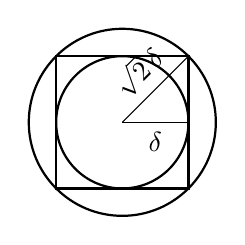
\begin{tikzpicture}[scale=0.8,baseline=(current bounding box.center)]
  \def\s{1.05}
  \draw[thick] (0,0) circle ({\s*1.414});
  \draw[thick] (-\s,-\s) rectangle (\s,\s);
  \draw[thick] (0,0) circle (\s);
  \draw (0,0) -- (\s,0) node[midway,below] {$\delta$};
  \draw (0,0) -- (\s,\s) node[midway,above,sloped] {$\sqrt{2}\,\delta$};
\end{tikzpicture}\caption{\relax}\label{fig:15-4}
\end{figure}

值得指出的是 $K^{*}(P_{0},\delta)$ 不可表示为 $0<\left|x-x_{0}\right|<\delta$，$0<\left|y-y_{0}\right|<\delta$．读者试想想，这是为什么．

设 $E$ 是平面上的点集，下面利用邻域来给出平面上任一点 $P_{0}$ 与点集 $E$ 的关系（见图~\ref{fig:15-5}）．

\begin{enumerate}[label=（\arabic*）,leftmargin=3.2em,itemsep=3pt,topsep=2pt]
\item \textbf{内点}：称 $P_{0}$ 是 $E$ 的内点，如果存在点 $P_{0}$ 的 $\delta$ 邻域完全含于 $E$ 内，即
\[
\exists\,\delta>0,\ \text{使}\ O\left(P_{0},\delta\right)\subset E.
\]
\item \textbf{外点}：称 $P_{0}$ 是 $E$ 的外点，如果存在点 $P_{0}$ 的 $\delta$ 邻域，其中不含 $E$ 的点，即
\[
\exists\,\delta>0,\ \text{使}\ O\left(P_{0},\delta\right)\cap E=\varnothing.
\]
\item \textbf{边界点}：称 $P_{0}$ 是 $E$ 的边界点，如果 $P_{0}$ 点的任意 $\delta$ 邻域中都既有 $E$ 的点，又有非 $E$ 的点，即
\[
\forall \delta>0,\ O\left(P_{0},\delta\right)\cap E\neq\varnothing\ \text{ 且 }\ O\left(P_{0},\delta\right)\setminus E\neq\varnothing.
\]
\item \textbf{聚点}：称 $P_{0}$ 是 $E$ 的聚点，如果 $P_{0}$ 点的任意 $\delta$ 空心邻域中都有 $E$ 的点，即
\[
\forall \delta>0,\ O^{*}\left(P_{0},\delta\right)\cap E\neq\varnothing.
\]
\end{enumerate}

\begin{figure}[htbp]
\centering
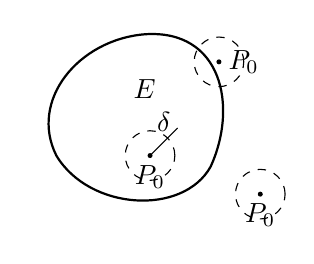
\begin{tikzpicture}[scale=0.7,baseline=(current bounding box.center)]
  \draw[thick] (0.2,1.6) .. controls (1.6,1.7) and (1.9,0.3) .. (1.4,-0.8)
    .. controls (0.9,-1.7) and (-0.8,-1.6) .. (-1.4,-0.6)
    .. controls (-1.9,0.4) and (-1.0,1.5) .. (0.2,1.6) -- cycle;
  \node at (0.2,0.6) {$E$};
  \coordinate (A) at (0.3,-0.6);
  \draw[dashed] (A) circle (0.45);
  \fill (A) circle (1.3pt) node[below] {$P_0$};
  \draw (A) -- ++(0.5,0.5) node[midway,above] {$\delta$};
  \coordinate (B) at (1.55,1.1);
  \draw[dashed] (B) circle (0.45);
  \fill (B) circle (1.3pt) node[right] {$P_0$};
  \coordinate (C) at (2.3,-1.3);
  \draw[dashed] (C) circle (0.45);
  \fill (C) circle (1.3pt) node[below] {$P_0$};
\end{tikzpicture}\caption{\relax}\label{fig:15-5}
\end{figure}

显然，$P_{0}$ 点是 $E$ 的内点、外点或边界点三者必居其一．$E$ 的内点必属于 $E$，$E$ 的外点必不属于 $E$，而 $E$ 的边界点和聚点可能属于 $E$，也可能不属于 $E$．$E$ 的内点是 $E$ 的聚点，外点不是 $E$ 的聚点，边界点可能是 $E$ 的聚点，也可能不是 $E$ 的聚点．

\begin{example}\label{ex:15-1-1}
给定集合 $E=\{(x,y)\mid x^{2}+y^{2}\leqslant 1\}$，则 $E$ 的内点构成的集合为 $\{(x,y)\mid x^{2}+y^{2}<1\}$；$E$ 的外点构成的集合为 $\{(x,y)\mid x^{2}+y^{2}>1\}$；$E$ 的边界点构成的集合为 $\{(x,y)\mid x^{2}+y^{2}=1\}$；$E$ 的聚点全体就是 $E$．
\end{example}

\begin{example}\label{ex:15-1-2}
设 $E=\{(x,y)\mid 0<x<1,0<y<1,x,y\ \text{都是有理数}\}$．则 $E$ 的内点集为空集 $\varnothing$，即 $E$ 没有内点；$E$ 的边界点集为 $\{(x,y)\mid 0\leqslant x\leqslant 1,0\leqslant y\leqslant 1\}$．$E$ 的所有边界点都是 $E$ 的聚点；所有非边界点是 $E$ 的外点．
\end{example}

下面是几种重要的平面点集．

\begin{enumerate}[label=（\arabic*）,leftmargin=3.2em,itemsep=3pt,topsep=2pt]
\item \textbf{开集}\quad 称平面点集 $E$ 是开集，如果 $E$ 的所有点都是内点．
\item \textbf{闭集}\quad 称平面点集 $E$ 是闭集，如果 $E$ 的所有聚点（如果有的话）都属于 $E$．
\item \textbf{连通集}\quad 称 $E$ 是连通集，如果 $E$ 中的任何两点都能用完全含于 $E$ 的由有限条直线段组成的折线连接起来（见图~\ref{fig:15-6}）．
\item \textbf{区域}\quad 连通的开集称为开区域，或简称区域．
\item \textbf{闭区域}\quad 区域连同它的边界点所成的集合称为闭区域．
\end{enumerate}

\begin{figure}[htbp]
\centering
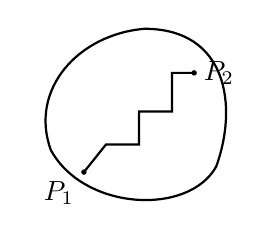
\begin{tikzpicture}[scale=0.7,baseline=(current bounding box.center)]
  \draw[thick] (0.2,1.6) .. controls (1.7,1.6) and (1.9,0.2) .. (1.5,-0.9)
    .. controls (1.0,-1.8) and (-0.9,-1.7) .. (-1.5,-0.6)
    .. controls (-1.9,0.5) and (-1.0,1.5) .. (0.2,1.6) -- cycle;
  \draw[thick] (-0.9,-1.0) -- (-0.5,-0.5) -- (0.1,-0.5) -- (0.1,0.1) -- (0.7,0.1) -- (0.7,0.8) -- (1.1,0.8);
  \fill (-0.9,-1.0) circle (1.4pt) node[below left] {$P_1$};
  \fill (1.1,0.8) circle (1.4pt) node[right] {$P_2$};
\end{tikzpicture}\caption{\relax}\label{fig:15-6}
\end{figure}

例如，邻域 $O(P_{0},\delta)$，$K(P_{0},\delta)$ 是开集，也是区域．集合
\[
\left\{(x,y)\mid \left(x-x_{0}\right)^{2}+\left(y-y_{0}\right)^{2}\leqslant\delta\right\},\quad
\left\{(x,y)\mid \left|x-x_{0}\right|\leqslant\delta,\left|y-y_{0}\right|\leqslant\delta\right\}
\]
都是闭集也是闭区域，其中 $\delta>0$．

例~\ref{ex:15-1-2} 中给出的集合 $E$ 既非开集也非闭集．二维平面 $\mathbf{R}^{2}$ 则既是区域又是闭区域，这是平面点集中除空集外唯一是开集又是闭集的集合．邻域和空心邻域是开集也是区域．

注意：区域总是开集，闭区域总是闭集．但反之未必．例如圆周
\[
\left\{(x,y)\mid x^{2}+y^{2}=\mathbf{R}^{2}\right\}
\]
是闭集，但不是闭区域，因为它没有内点，因而不是由某个开集及其边界构成的（图~\ref{fig:15-7}）．又如
\[
\left\{(x,y)\mid xy>0\right\}
\]
是开集，但不是区域，因为它不连通（图~\ref{fig:15-8}）．

\begin{figure}[htbp]
\centering
\begin{tikzpicture}[scale=0.7,baseline=(current bounding box.center)]
  \draw[{-Latex}] (-2.4,0) -- (2.6,0) node[below left] {$x$};
  \draw[{-Latex}] (0,-2.1) -- (0,2.3) node[left] {$y$};
  \node[below left] at (0,0) {$O$};
  \draw[thick] (0,0) circle (1.7);
  \node[below right] at (1.7,0) {$R$};
\end{tikzpicture}\caption{\relax}\label{fig:15-7}
\end{figure}

\begin{figure}[htbp]
\centering
\begin{tikzpicture}[scale=0.7,baseline=(current bounding box.center)]
  \draw[{-Latex}] (-2.4,0) -- (2.6,0) node[below left] {$x$};
  \draw[{-Latex}] (0,-2.3) -- (0,2.3) node[left] {$y$};
  \node[below left] at (0,0) {$O$};
  \fill[pattern=north east lines] (0.3,0.3) -- (2.0,0.3) -- (0.3,2.0) -- cycle;
  \fill[pattern=north east lines] (-0.3,-0.3) -- (-2.0,-0.3) -- (-0.3,-2.0) -- cycle;
\end{tikzpicture}\caption{\relax}\label{fig:15-8}
\end{figure}

回忆一元函数极限与连续的理论，开区间与闭区间的概念是十分重要的．现在我们看到，区域是直线上开区间在平面的对应物，有界闭区域是直线上闭区间在平面的对应物．把区域、闭区域的多样性与直线的开区间、闭区间相比较，可看到多元问题的确较一元问题复杂得多．

下面给出平面点列的极限概念．

\begin{definition}\label{def:15-1}
设 $\{P_{n}\}$ 是平面上的点列，其中 $P_{n}=(x_{n},y_{n})$．又 $P_{0}=(x_{0},y_{0})$ 是平面上的一点．若对任给的正数 $\varepsilon$，存在正整数 $N$，当 $n>N$ 时，有
\begin{equation}
r\left(P_{n},P_{0}\right)=\sqrt{\left(x_{n}-x_{0}\right)^{2}+\left(y_{n}-y_{0}\right)^{2}}<\varepsilon,
\tag{1}
\end{equation}
则称点列 $\{P_{n}\}$ 收敛到点 $P_{0}$，或称点列 $\{P_{n}\}$ 当 $n$ 趋于无穷时的极限为 $P_{0}$，记为
\[
\lim_{n\to\infty}P_{n}=P_{0}\quad\text{或}\quad P_{n}\to P_{0}\ (n\to\infty).
\]
\end{definition}

（1）式描述的是两点 $P_{n}$ 和 $P_{0}$ 之间的距离小于 $\varepsilon$，这种描述是实数极限 $\lim\limits_{n\to\infty}x_{n}=a$ 的定义中 $\left|x_{n}-a\right|<\varepsilon$ 的直接推广．如果用邻域来描述，则（1）式等价于
\[
P_{n}\in O\left(P_{0},\varepsilon\right).
\]
因此平面上点列 $\{P_{n}\}$ 收敛到 $P_{0}$ 的几何意义是：对 $P_{0}$ 的任意邻域 $O(P_{0},\varepsilon)$，至多有点列的有限项 $P_{1},\cdots,P_{N}$ 不在邻域 $O(P_{0},\varepsilon)$ 内，其余的 $P_{n}$ 全部落在 $P_{0}$ 的邻域 $O(P_{0},\varepsilon)$ 内．

不难证明下列各式是等价的，请读者写出它们的证明．

\begin{enumerate}[label=(\roman*),leftmargin=3.2em,itemsep=2pt,topsep=2pt]
\item $\displaystyle\lim_{n\to\infty}P_{n}=P_{0}$；
\item $\displaystyle\lim_{n\to\infty}r(P_{n},P_{0})=0$；
\item $\displaystyle\lim_{n\to\infty}x_{n}=x_{0}$，且 $\displaystyle\lim_{n\to\infty}y_{n}=y_{0}$．
\end{enumerate}

注意到（ii）和（iii）就是实数列的极限，因此上述等价性使得我们可以方便地应用实数的极限理论．例如由实数列极限的唯一性立即可知平面点列的极限若存在则是唯一的．

\begin{figure}[htbp]
\centering
\begin{tikzpicture}[scale=0.7,baseline=(current bounding box.center)]
  \def\R{1.3}
  \coordinate (P0) at (2.4,2.2);
  \draw[{-Latex}] (0,0) -- (4.3,0) node[below left] {$x$};
  \draw[{-Latex}] (0,0) -- (0,4) node[left] {$y$};
  \node[below left] at (0,0) {$O$};
  \draw[pattern=north east lines] (P0) circle (\R);
  \draw[dashed,thick] (P0) circle (\R);
  \draw[dashed] (P0) -- ++(\R,0) node[midway,above] {$\varepsilon$};
  \fill (P0) circle (1.4pt) node[left] {$P_0$};
\end{tikzpicture}\caption{\relax}\label{fig:15-9}
\end{figure}

\begin{example}\label{ex:15-1-3}
设 $P_{n}=\left\{\dfrac{1}{n},\sin\dfrac{1}{n}\right\}$，$P_{0}=(0,0)$，则 $\lim\limits_{n\to\infty}P_{n}=P_{0}$．设 $P_{n}=\left\{\left(1+\dfrac{1}{n}\right)^{n},\cos\dfrac{1}{n}\right\}$，$P_{0}=(\mathrm{e},1)$，则 $\lim\limits_{n\to\infty}P_{n}=P_{0}$．
\end{example}

实数的连续性、完备性和有界闭集的紧致性（前面我们只讲过闭区间）是一元函数微积分的基础．连续性涉及实数的顺序，这里不多讲了．下面我们将完备性和紧致性推广到二维情形，它们同样是二元函数微积分的基础．

\begin{theorem}[柯西收敛原理]\label{thm:15-1}
平面点列 $\{P_{n}\}$ 收敛的充分必要条件是：对任给的正数 $\varepsilon$，存在正整数 $N$，当 $n$，$m>N$ 时，有
\begin{equation}
r\left(P_{n},P_{m}\right)<\varepsilon.
\tag{2}
\end{equation}
\end{theorem}

\begin{proof}
必要性．设平面点列 $\{P_{n}\}$ 收敛于 $P_{0}$，由极限定义知，对任给的 $\varepsilon>0$，存在 $N$，当 $n>N$ 时有
\[
r\left(P_{n},P_{0}\right)<\frac{\varepsilon}{2}.
\]
于是由距离的三角不等式，当 $n$，$m>N$ 时有
\[
r\left(P_{n},P_{m}\right)\leqslant r\left(P_{n},P_{0}\right)+r\left(P_{0},P_{m}\right)<\frac{\varepsilon}{2}+\frac{\varepsilon}{2}=\varepsilon.
\]

充分性．设 $P_{n}(x_{n},y_{n})$ 满足已知条件，即对任给的 $\varepsilon>0$，存在 $N$，当 $n$，$m>N$ 时，有
\[
r\left(P_{n},P_{m}\right)=\sqrt{\left(x_{n}-x_{m}\right)^{2}+\left(y_{n}-y_{m}\right)^{2}}<\varepsilon,
\]
从而有
\[
\left|x_{n}-x_{m}\right|<\varepsilon,\quad\left|y_{n}-y_{m}\right|<\varepsilon.
\]
由数列极限的柯西收敛原理知，数列 $\{x_{n}\}$ 和 $\{y_{n}\}$ 都收敛，设分别收敛到 $x_{0},y_{0}$：$x_{n}\to x_{0}$，$y_{n}\to y_{0}$．因此 $P_{n}(x_{n},y_{n})\to P_{0}(x_{0},y_{0})\ (n\to\infty)$，故平面点列 $\{P_{n}\}$ 收敛．定理~\ref{thm:15-1} 证完．
\end{proof}

对比第九章 §3 数列的柯西收敛原理的证明，我们看到，这里必要性的证明，用的是数列情形的证明方法，而充分性的证明则用的是数列情形的结果．

\begin{definition}\label{def:15-2}
称平面点列为有界的，如果存在正数 $M$，使
\[
r\left(P_{n},O\right)\leqslant M.
\]
\end{definition}

容易看出，点列 $\{P_{n}(x_{n},y_{n})\}$ 有界，当且仅当数列 $\{x_{n}\}$，$\{y_{n}\}$ 均有界．

\begin{theorem}[波尔察诺--魏尔斯特拉斯致密性定理]\label{thm:15-2}
若点列 $\{P_{n}\}$ 有界，则 $\{P_{n}\}$ 必有收敛子列．
\end{theorem}

\begin{proof}
相继地用两次实数列的致密性定理．已知点列 $\{P_{n}\}$ 有界，$P_{n}=(x_{n},y_{n})$．这时实数列 $\{x_{n}\}$ 和 $\{y_{n}\}$ 有界．因此 $\{x_{n}\}$ 有收敛子列 $\{x_{n_{k}}\}$，即 $x_{n_{k}}\to x_{0}\ (k\to\infty)$．由相应的实数列 $\{y_{n_{k}}\}$ 有界，知它有收敛子列 $\{y_{n_{k_{l}}}\}$，即 $y_{n_{k_{l}}}\to y_{0}\ (l\to\infty)$，而对应的 $\{x_{n_{k_{l}}}\}$ 是 $\{x_{n_{k}}\}$ 的子列，因此 $x_{n_{k_{l}}}\to x_{0}\ (l\to\infty)$．于是 $P_{n_{k_{l}}}=(x_{n_{k_{l}}},y_{n_{k_{l}}})$ 构成的平面点列 $\{P_{n_{k_{l}}}\}$ 是 $\{P_{n}\}$ 的子列，它有极限 $P_{0}(x_{0},y_{0})$，定理~\ref{thm:15-2} 证完．
\end{proof}

定理~\ref{thm:15-2} 的证明，用的是一元的结果．

\begin{theorem}[矩形套定理]\label{thm:15-3}
设 $D_{n}=\left\{(x,y)\mid a_{n}\leqslant x\leqslant b_{n},c_{n}\leqslant y\leqslant d_{n}\right\}$ 是平面上的闭矩形序列（图~\ref{fig:15-10}），满足
\[
\begin{aligned}
1^{\circ}\quad & a_{n}\leqslant a_{n+1}\leqslant b_{n+1}\leqslant b_{n},\ c_{n}\leqslant c_{n+1}\leqslant d_{n+1}\leqslant d_{n},\ n=1,2,\cdots;\\
2^{\circ}\quad & b_{n}-a_{n}\to 0\ \ (n\to\infty),\ d_{n}-c_{n}\to 0\ \ (n\to\infty).
\end{aligned}
\]
则存在唯一的一点 $P_{0}(x_{0},y_{0})$，使得 $P_{0}\in\bigcap\limits_{n=1}^{\infty}D_{n}$，即
\[
a_{n}\leqslant x_{0}\leqslant b_{n},\quad c_{n}\leqslant y_{0}\leqslant d_{n},\quad n=1,2,\cdots.
\]
\end{theorem}

\begin{figure}[htbp]
\centering
\begin{tikzpicture}[scale=0.7,baseline=(current bounding box.center)]
  \draw[{-Latex}] (0,0) -- (4.6,0) node[below left] {$x$};
  \draw[{-Latex}] (0,0) -- (0,4.0) node[left] {$y$};
  \node[below left] at (0,0) {$O$};
  \draw[thick] (0.6,0.6) rectangle (4.2,3.4);
  \draw[thick] (1.0,1.0) rectangle (3.6,2.9);
  \draw[thick] (1.7,1.6) rectangle (2.9,2.4);
  \draw[dashed] (0.6,0) -- (0.6,0.6);
  \draw[dashed] (1.0,0) -- (1.0,1.0);
  \draw[dashed] (3.6,0) -- (3.6,2.9);
  \draw[dashed] (4.2,0) -- (4.2,3.4);
  \draw[dashed] (0,0.6) -- (0.6,0.6);
  \draw[dashed] (0,1.0) -- (1.0,1.0);
  \draw[dashed] (0,2.9) -- (3.6,2.9);
  \draw[dashed] (0,3.4) -- (4.2,3.4);
  \node[below] at (0.6,0) {$a_1$};
  \node[below] at (1.0,0) {$a_2$};
  \node[below] at (3.6,0) {$b_2$};
  \node[below] at (4.2,0) {$b_1$};
  \node[left] at (0,3.4) {$d_1$};
  \node[left] at (0,2.9) {$d_2$};
  \node[left] at (0,1.0) {$c_2$};
  \node[left] at (0,0.6) {$c_1$};
\end{tikzpicture}\caption{\relax}\label{fig:15-10}
\end{figure}

\begin{proof}
只要对区间套 $\{[a_{n},b_{n}]\}$ 和 $\{[c_{n},d_{n}]\}$ 分别用区间套定理即可．
\end{proof}

最后我们用矩形套定理来证明平面上的有限覆盖定理．先给出覆盖的定义．

\begin{definition}\label{def:15-3}
设 $\zeta$ 是由开集构成的集族．称 $\zeta$ 是集合 $E$ 的一个覆盖，如果对任意点 $P\in E$，存在开集 $G\in\zeta$，使 $P\in G$，即 $E\subset\bigcup\limits_{G\in\zeta}G$．
\end{definition}

\begin{theorem}[博雷尔有限覆盖定理]\label{thm:15-4}
设 $E$ 是平面上的有界闭集，$\zeta$ 是 $E$ 的一个覆盖，则 $\zeta$ 中存在有限个开集 $G_{1},G_{2},\cdots,G_{n}$，使 $E\subset\bigcup\limits_{i=1}^{n}G_{i}$．
\end{theorem}

定理~\ref{thm:15-4} 说的是有界闭集 $E$ 的任何覆盖，必存在有限子覆盖．定理的证明很难用一元的结果，只好用一元的方法．

\begin{proof}[定理~\ref{thm:15-4} 的证明]
用反证法．已知 $E$ 是平面上的有界闭集，因此存在闭矩形
\[
D=\left\{(x,y)\mid a\leqslant x\leqslant b,c\leqslant y\leqslant d\right\},
\]
使 $E$ 含于 $D$．设 $E$ 不能被 $\zeta$ 中有限个开集所覆盖．用 $D$ 的对边中点的连线
\[
x=\frac{a+b}{2},\quad y=\frac{c+d}{2}
\]
把矩形 $D$ 分成四个相等的闭矩形，则其中至少有一个闭矩形，它包含 $E$ 的部分不能被 $\zeta$ 中有限个开集所覆盖，记这个闭矩形为
\[
D_{1}=\left\{(x,y)\mid a_{1}\leqslant x\leqslant b_{1},c_{1}\leqslant y\leqslant d_{1}\right\}.
\]
再用 $D_{1}$ 对边中点的连线把矩形 $D_{1}$ 分成四个相等的闭矩形，其中至少有一个闭矩形，它包含 $E$ 的部分不能被 $\zeta$ 中有限个开集所覆盖，记这个闭矩形为 $D_{2}$．如此继续下去，得闭矩形序列 $\{D_{n}\}$，满足
\[
\begin{aligned}
1^{\circ}\quad & D_{n}\supseteq D_{n+1},\ n=1,2,\cdots;\\
2^{\circ}\quad & \text{矩形的边长分别为}\ b_{n}-a_{n},\ d_{n}-c_{n},\ \text{且}\\
& b_{n}-a_{n}=\frac{b-a}{2^{n}}\to 0,\quad d_{n}-c_{n}=\frac{d-c}{2^{n}}\to 0\ \ (n\to\infty);\\
3^{\circ}\quad & D_{n}\cap E\ \text{不能被}\ \zeta\ \text{中有限个开集所覆盖}.
\end{aligned}
\]
由矩形套定理，存在唯一的点 $P_{0}(x_{0},y_{0})$ 使得 $P_{0}\in\bigcap\limits_{n=1}^{\infty}D_{n}$，又因为 $D_{n}\cap E\neq\varnothing$，则存在 $P_{n}(x_{n},y_{n})\in D_{n}\cap E$，即
\[
a_{n}\leqslant x_{n}\leqslant b_{n},\quad c_{n}\leqslant y_{n}\leqslant d_{n},\quad n=1,2,\cdots,
\]
而且
\[
\lim_{n\to\infty}a_{n}=\lim_{n\to\infty}b_{n}=x_{0},\quad \lim_{n\to\infty}c_{n}=\lim_{n\to\infty}d_{n}=y_{0},
\]
故
\[
\lim_{n\to\infty}x_{n}=x_{0},\quad\lim_{n\to\infty}y_{n}=y_{0}.
\]
由于 $E$ 是闭集，故 $P_{0}(x_{0},y_{0})\in E$．根据 $\zeta$ 是 $E$ 的覆盖，则存在 $G\in\zeta$，使 $P_{0}\in G$．因为 $G$ 是开集，所以存在 $P_{0}$ 的 $\delta$ 邻域
\[
\Delta=\left\{(x,y)\mid \left|x-x_{0}\right|<\delta,\left|y-y_{0}\right|<\delta\right\},
\]
使得 $\Delta\subset G$．注意到 $\{a_{n}\}$ 和 $\{b_{n}\}$ 的极限为 $x_{0}$，$\{c_{n}\}$ 和 $\{d_{n}\}$ 的极限为 $y_{0}$，从而存在 $N$，当 $n>N$ 时有
\[
x_{0}-\delta<a_{n}<b_{n}<x_{0}+\delta,\quad y_{0}-\delta<c_{n}<d_{n}<y_{0}+\delta,
\]
所以 $D_{n}\subset\Delta\subset G$，即 $D_{n}\cap E$ 被 $\zeta$ 的一个集 $G$ 所覆盖．这与前面的性质 $3^{\circ}$ 矛盾．因此 $\zeta$ 中必有有限个开集覆盖 $E$．定理~\ref{thm:15-4} 证完．
\end{proof}

回忆第九章 §2，知定理~\ref{thm:15-4} 说明平面上有界闭集是紧致的．注意与直线上的有限覆盖定理一样，定理中 $E$ 是有界和闭的条件缺一不可．事实上取
\[
E=\left\{(x,y)\mid x^{2}+y^{2}<1\right\},
\]
则 $E$ 是有界的，但非闭．令
\[
G_{n}=\left\{(x,y)\mid x^{2}+y^{2}<\left(1-\frac{1}{n}\right)^{2}\right\}.
\]
显然 $\zeta=\left\{G_{n}\mid n=2,3,\cdots\right\}$ 是 $E$ 的覆盖，但不存在 $E$ 的有限子覆盖．又如取
\[
E=\left\{(x,y)\mid x\geqslant 0,y\geqslant 0\right\},
\]
则 $E$ 是闭集，但无界．取
\[
G_{n}=\left\{(x,y)\mid x^{2}+y^{2}<n^{2}\right\}.
\]
显然 $\zeta=\left\{G_{n}\mid n=1,2,\cdots\right\}$ 是 $E$ 的覆盖，但不存在 $E$ 的有限子覆盖．

\begin{xiti}
\item 设 $\{P_{n}=(x_{n},y_{n})\}$ 是平面点列，$P_{0}=(x_{0},y_{0})$ 是平面上的点．证明 $\lim\limits_{n\to\infty}P_{n}=P_{0}$ 的充要条件是 $\lim\limits_{n\to\infty}x_{n}=x_{0}$，且 $\lim\limits_{n\to\infty}y_{n}=y_{0}$．
\item 设平面点列 $\{P_{n}\}$ 收敛，证明 $\{P_{n}\}$ 有界．
\item 判别下列平面点集哪些是开集、闭集、有界集或区域，并分别指出它们的聚点：
\begin{ziti}
\item $E=\left\{(x,y)\mid y<x^{2}\right\}$；
\item $E=\left\{(x,y)\mid x^{2}+y^{2}\neq 1\right\}$；
\item $E=\left\{(x,y)\mid xy\neq 0\right\}$；
\item $E=\left\{(x,y)\mid xy=0\right\}$；
\item $E=\left\{(x,y)\mid 0\leqslant y\leqslant 2,2y\leqslant x\leqslant 2y+2\right\}$；
\item $E=\left\{(x,y)\mid y=\sin\dfrac{1}{x},x>0\right\}$；
\item $E=\left\{(x,y)\mid x^{2}+y^{2}=1\ \text{或}\ y=0,0\leqslant x\leqslant 1\right\}$；
\item $E=\left\{(x,y)\mid x,y\ \text{均为整数}\right\}$．
\end{ziti}
\item 设 $F$ 是闭集，$G$ 是开集，证明 $F\setminus G$ 是闭集，$G\setminus F$ 是开集．
\item 证明开集的余集是闭集．
\item 设 $E$ 是平面点集．证明 $P_{0}$ 是 $E$ 的聚点的充要条件是 $E$ 中存在点列 $\{P_{n}\}$，满足 $P_{n}\neq P_{0}\ (n=1,2,\cdots)$ 且 $\lim\limits_{n\to\infty}P_{n}=P_{0}$．
\item 用平面上的有限覆盖定理证明平面上的致密性定理．
\item 用平面上的致密性定理证明平面点列的柯西收敛原理．
\item 设 $E$ 是平面点集，如果集合 $E$ 的任一覆盖都有有限子覆盖，则称 $E$ 是紧集．证明紧集是有界闭集．
\item 设 $E$ 是平面上的有界闭集，$d(E)$ 是 $E$ 的直径，即
\[
d(E)=\sup_{P^{\prime},P^{\prime\prime}\in E}r\left(P^{\prime},P^{\prime\prime}\right).
\]
求证：存在 $P_{1}$，$P_{2}\in E$，使得 $r(P_{1},P_{2})=d(E)$．
\item 仿照平面点集，叙述 $n$ 维欧氏空间中点集的有关概念（如邻域、极限、开集、聚点、闭集、区域、有界以及一些基本定理等）．
\item 叙述并证明三维空间的波尔察诺--魏尔斯特拉斯致密性定理．
\end{xiti}

\section{多元函数的极限与连续性}

\subsection{多元函数的概念}

仿照一元函数的情形，我们先给出二元函数的定义．

\begin{definition}\label{def:15-4}
设 $E$ 是平面点集．如果存在对应关系 $f$，使得对任意的 $(x,y)\in E$，按这个对应关系 $f$，有唯一的实数 $u$ 与之对应，则称 $f$ 为定义在 $E$ 上的二元函数，记为
\[
\begin{aligned}
f\colon E&\to\mathbf{R},\\
(x,y)&\to u=f(x,y).
\end{aligned}
\]
称 $E$ 为函数 $f$ 的定义域，$x$、$y$ 称为函数 $f$ 的自变量，而 $u$ 则称为因变量．$u=f(x,y)$ 是函数 $f$ 在 $(x,y)$ 点所对应的函数值，全体函数值的集合 $f(E)$ 称为函数 $f$ 的值域．
\end{definition}

在数学分析中，为了方便，我们也常把二元函数记为
\[
u=f(x,y),\quad(x,y)\in E
\]
或
\[
u=f(P),\quad P\in E.
\]

\begin{example}\label{ex:15-2-1}
半径为 $r$，高为 $h$ 的圆柱体的体积 $u$ 可表为
\[
u=\pi r^{2}h.
\]
根据实际意义，它的定义域是 $r>0$，$h>0$，值域是 $(0,+\infty)$．
\end{example}

\begin{example}\label{ex:15-2-2}
函数 $u=\sqrt{R^{2}-\left(x^{2}+y^{2}\right)}$ 的定义域是 $x^{2}+y^{2}\leqslant R^{2}$，值域是 $[0,R]$．
\end{example}

\begin{example}\label{ex:15-2-3}
函数 $u=\arcsin\dfrac{x}{a}+\arcsin\dfrac{y}{b}$ 的定义域是 $-a\leqslant x\leqslant a$，$-b\leqslant y\leqslant b$，值域是 $[-\pi,\pi]$．
\end{example}

在一元函数的微积分中，几何图形给了我们很直观的认识，对分析起着重要的作用．二元函数也是如此，几何直观仍是十分重要的．下面给出二元函数的几何表示．

空间点集
\[
\left\{(x,y,z)\mid z=f(x,y),(x,y)\in E\right\}
\]
称为函数 $z=f(x,y)$ 的图形．一般来说它构成一块空间曲面，定义域 $E$ 就是这块曲面在 $Oxy$ 平面上的投影．曲面的特点是，过定义域每一点平行于 $z$ 轴的直线只与曲面相交于一点．

例~\ref{ex:15-2-2} 中函数的图形是以原点为中心以 $R$ 为半径的上半球面，如图~\ref{fig:15-11} 所示．

从解析几何知道，$z=x^{2}+y^{2}$ 的图形是椭圆抛物面（图~\ref{fig:15-12}）．

\begin{figure}[htbp]
\centering
\begin{minipage}[c]{0.48\textwidth}\centering
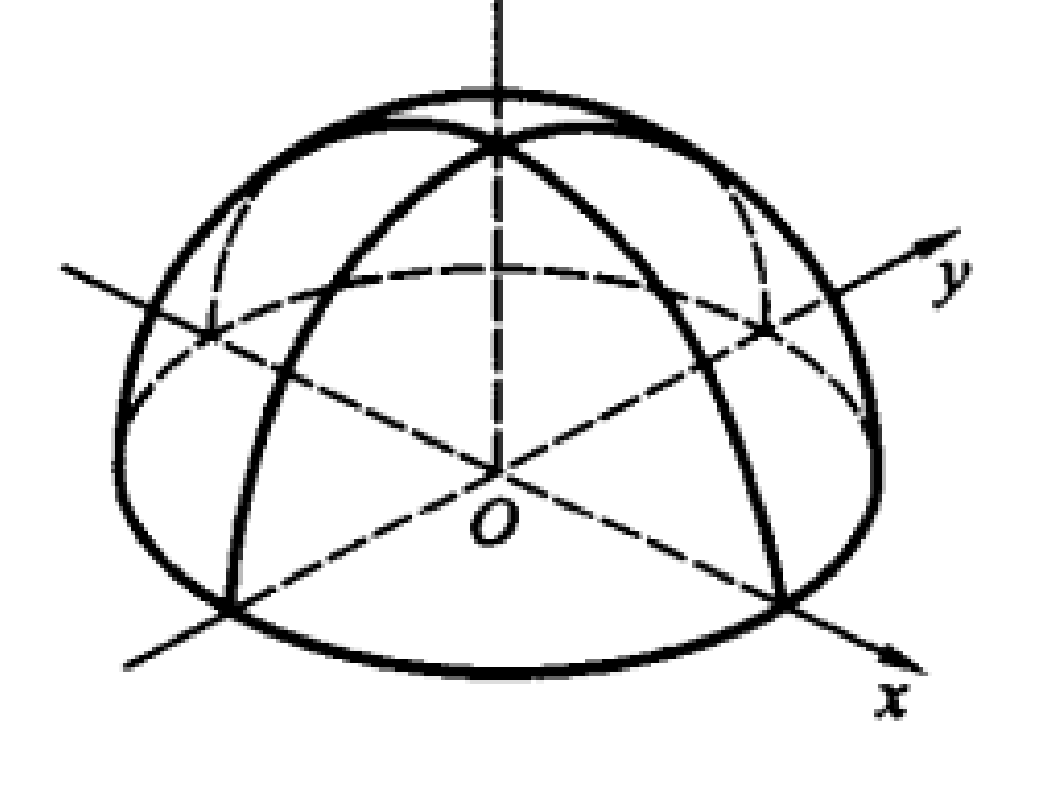
\includegraphics[width=0.72\textwidth]{work/figures/fig15-11}\caption{\relax}\label{fig:15-11}
\end{minipage}\hfill
\begin{minipage}[c]{0.48\textwidth}\centering
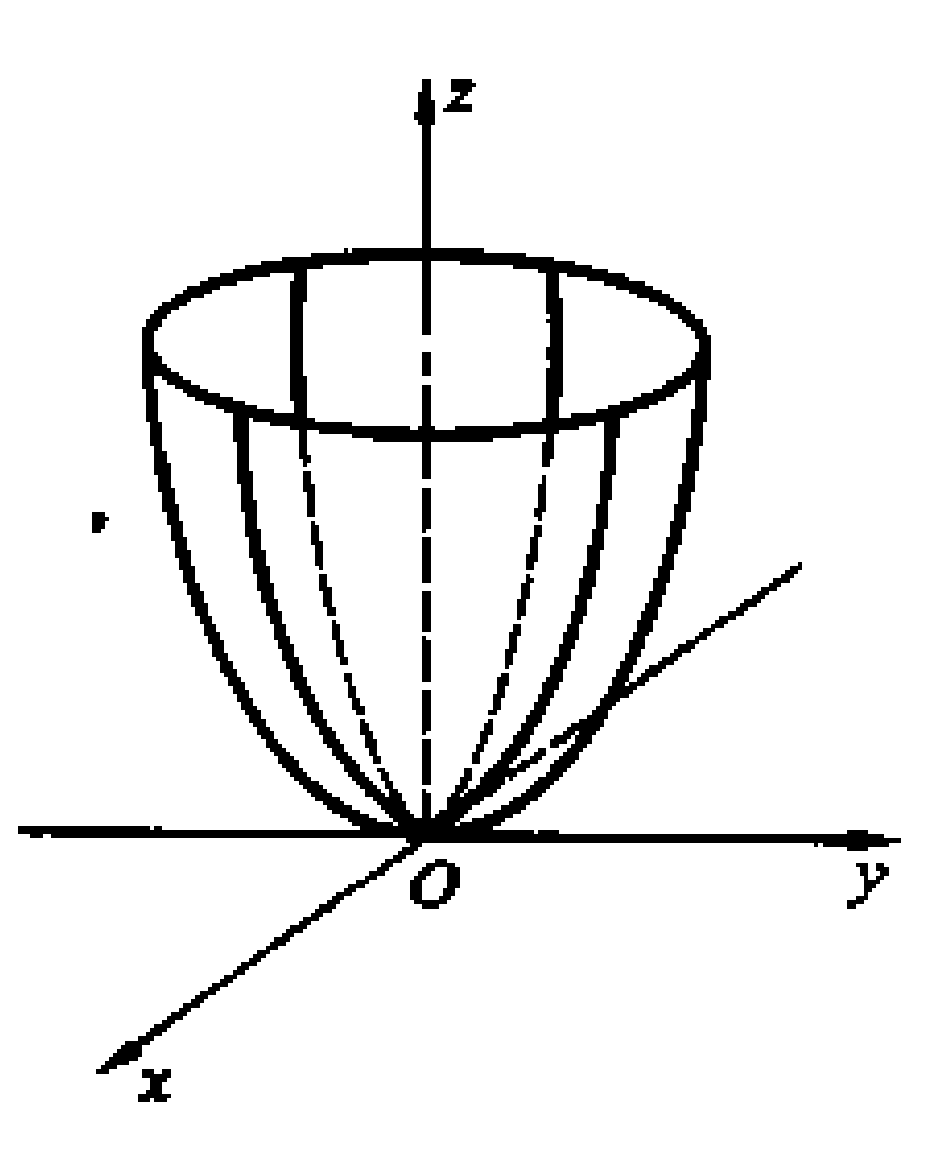
\includegraphics[width=0.72\textwidth]{work/figures/fig15-12}\caption{\relax}\label{fig:15-12}
\end{minipage}
\end{figure}

$z=\sqrt{x^{2}+y^{2}}$ 的图形是锥面（图~\ref{fig:15-13}）．而 $z=xy$ 的图形是双曲抛物面（图~\ref{fig:15-14}）．

\begin{figure}[htbp]
\centering
\begin{minipage}[c]{0.42\textwidth}\centering
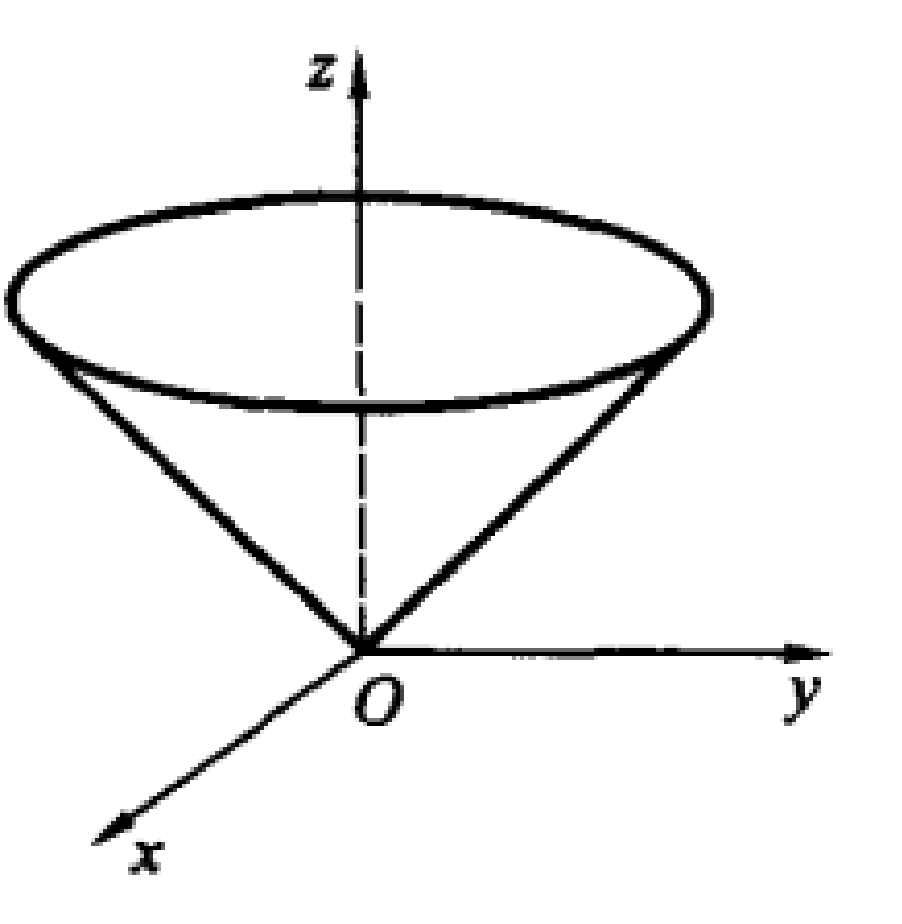
\includegraphics[width=0.72\textwidth]{work/figures/fig15-13}\caption{\relax}\label{fig:15-13}
\end{minipage}\hfill
\begin{minipage}[c]{0.55\textwidth}\centering
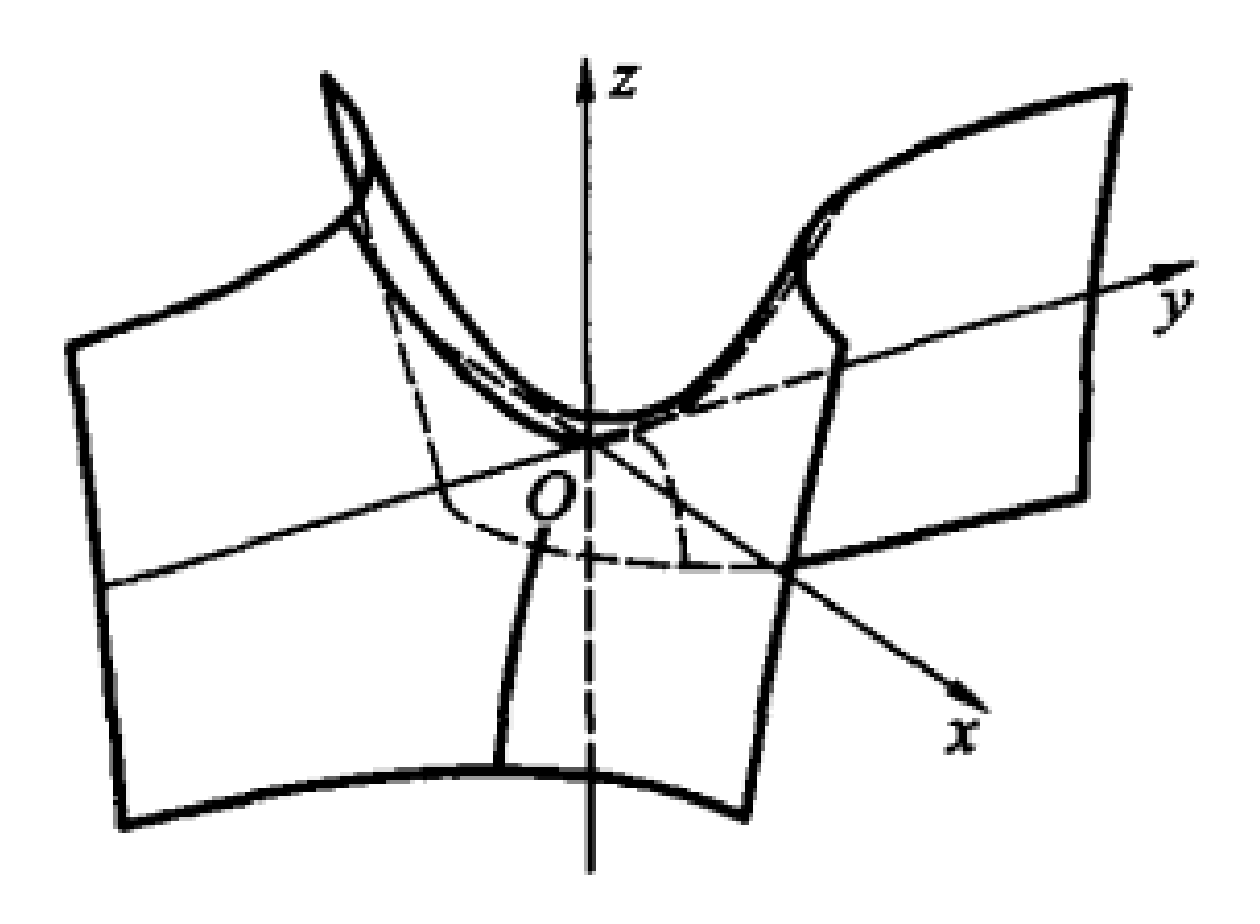
\includegraphics[width=0.9\textwidth]{work/figures/fig15-14}\caption{\relax}\label{fig:15-14}
\end{minipage}
\end{figure}

二元函数的定义很容易推广到多元函数的情形，只要在定义中将二元有序数对 $(x,y)$ 改为 $n$ 元有序数组 $(x_{1},x_{2},\cdots,x_{n})$ 即可．在此不详细叙述．我们简记 $n$ 元函数为
\[
u=f(x_{1},x_{2},\cdots,x_{n}),\ (x_{1},x_{2},\cdots,x_{n})\in E,
\]
或
\[
u=f(P),\ P\in E,
\]
其中
\[
E\subset\mathbf{R}^{n}=\left\{\left(x_{1},x_{2},\cdots,x_{n}\right)\mid -\infty<x_{i}<+\infty,i=1,2,\cdots,n\right\}.
\]
后一种写法是点的形式，它在形式上使多元函数与一元函数保持一致，以便于用类比的方法，把低维的（一元或二元的）结果及研究方法推广到高维．

\subsection{二元函数的极限}

\begin{definition}\label{def:15-5}
设 $f$ 在 $P_{0}(x_{0},y_{0})$ 的某个空心邻域内有定义，$A$ 是一个确定的数．如果对任给的 $\varepsilon>0$，存在 $\delta>0$，使得当 $0<r(P,P_{0})<\delta$ 时，有
\[
\left|f(P)-A\right|<\varepsilon,
\]
那么称 $A$ 是二元函数 $f$ 当 $P\to P_{0}$ 时的极限，记为
\[
\lim_{P\to P_{0}}f(P)=A,
\]
或
\[
\lim_{\substack{x\to x_{0}\\ y\to y_{0}}}f(x,y)=A.
\]
\end{definition}

注意到 $0<r(P,P_{0})<\delta$ 等价于 $P\in O^{*}(P_{0},\delta)$，而 $\left|f(P)-A\right|<\varepsilon$ 等价于 $f(P)\in(A-\varepsilon,A+\varepsilon)=O(A,\varepsilon)$（直线上的邻域）．因此，上述定义又可以用邻域的语言叙述为：对任给的 $\varepsilon>0$，存在 $\delta>0$，只要 $P\in O^{*}(P_{0},\delta)$，就有
\[
f(P)\in O(A,\varepsilon).
\]
由于圆邻域和方邻域可以互相包含，因此上述定义也可叙述为：对任给的 $\varepsilon>0$，存在 $\delta>0$，只要 $P\in K^{*}(P_{0},\delta)$，就有
\[
f(P)\in O(A,\varepsilon).
\]
但在解题时，还是用下述的不等式说法方便：
\[
\lim_{\substack{x\to x_{0}\\ y\to y_{0}}}f(x,y)=A,
\]
当且仅当对任给的 $\varepsilon>0$，存在 $\delta>0$，只要 $0<\sqrt{\left(x-x_{0}\right)^{2}+\left(y-y_{0}\right)^{2}}<\delta$，就有
\[
\left|f(x,y)-A\right|<\varepsilon.
\]
或当且仅当对任给的 $\varepsilon>0$，存在 $\delta>0$，只要 $\left|x-x_{0}\right|<\delta$，$\left|y-y_{0}\right|<\delta$，$(x,y)\neq(x_{0},y_{0})$，有
\[
\left|f(x,y)-A\right|<\varepsilon.
\]

\begin{example}\label{ex:15-2-4}
设 $f(x,y)=xy\dfrac{x^{2}-y^{2}}{x^{2}+y^{2}}$，证明 $\lim\limits_{\substack{x\to0\\y\to0}}f(x,y)=0$．
\end{example}

\begin{proof}[证明]
因为
\[
\begin{aligned}
\left|f(x,y)-0\right|&=\left|\,xy\,\dfrac{x^{2}-y^{2}}{x^{2}+y^{2}}\right|\leqslant\left|\,xy\,\right|\dfrac{x^{2}+y^{2}}{x^{2}+y^{2}}\\
&=\left|\,xy\right|\leqslant\dfrac{x^{2}+y^{2}}{2},
\end{aligned}
\]
所以对任给的 $\varepsilon>0$，要 $\left|f(x,y)-0\right|<\varepsilon$，只要 $\dfrac{x^{2}+y^{2}}{2}<\varepsilon$．取 $\delta=\sqrt{2\varepsilon}$，则当 $0<\sqrt{x^{2}+y^{2}}<\delta$ 时，有
\[
\left|f(x,y)-0\right|\leqslant\dfrac{x^{2}+y^{2}}{2}<\varepsilon.
\]
也可以取 $\delta=\sqrt{\varepsilon}$，则只要 $\left|x\right|<\delta$，$\left|y\right|<\delta$，$(x,y)\neq(0,0)$，就有
\[
\left|f(x,y)-0\right|\leqslant\left|xy\right|<\delta^{2}=\varepsilon.
\]
回忆一元的情形，知道这里用的是“适当放大法”．
\end{proof}

二元函数极限 $\lim\limits_{P\to P_{0}}f(P)=A$ 的几何意义是：对任给的 $\varepsilon>0$，必存在点 $P_{0}$ 的 $\delta$ 空心邻域 $O^{*}(P_{0},\delta)$，使得经过 $f$ 的对应，空心邻域中所有点的像全部落在区间 $(A-\varepsilon,A+\varepsilon)$ 之中（图~\ref{fig:15-15}），即
\[
f\left(O^{*}\left(P_{0},\delta\right)\right)\subset\left(A-\varepsilon,A+\varepsilon\right).
\]

\begin{figure}[htbp]
\centering
\begin{tikzpicture}[scale=0.72,baseline=(current bounding box.center)]
  \draw[thick] (0,2.2) .. controls (1.6,2.3) and (2.0,1.2) .. (1.7,0.4)
    .. controls (1.5,-0.2) and (0.5,0.1) .. (0.2,-0.4)
    .. controls (-0.1,-1.0) and (-1.3,-0.9) .. (-1.5,0.0)
    .. controls (-1.7,1.0) and (-1.0,2.1) .. (0,2.2) -- cycle;
  \node at (1.1,1.4) {$\Omega$};
  \coordinate (P0) at (-0.3,1.2);
  \draw[thick] (P0) circle (0.5);
  \fill (P0) circle (1.4pt) node[above right] {$P_0$};
  \draw (P0) -- ++(180:0.5) node[midway,above] {$\delta$};
  \draw[{-Latex},thick] (0.2,-0.4) .. controls (0.5,-1.0) .. (0.9,-1.4) node[midway,right] {$f$};
  \draw (-0.6,-1.6) -- (2.6,-1.6);
  \draw (-0.2,-1.75) -- (-0.2,-1.45);
  \draw (2.0,-1.75) -- (2.0,-1.45);
  \draw (0.9,-1.75) -- (0.9,-1.45);
  \fill (0.9,-1.6) circle (1.4pt) node[below] {$A$};
  \node[below] at (-0.2,-1.75) {$A-\varepsilon$};
  \node[below] at (2.0,-1.75) {$A+\varepsilon$};
\end{tikzpicture}\caption{\relax}\label{fig:15-15}
\end{figure}

借助于几何直观，我们可以看到平面上的点 $P\to P_{0}$ 的意义远比直线上 $x\to x_{0}$ 要复杂得多．在直线上，$x\to x_{0}$ 只有左、右两个方向，而在平面上 $P\to P_{0}$ 的方向有无穷多个，且路径也有无穷多种（图~\ref{fig:15-16}）．例如 $P$ 点可沿直线趋于 $P_{0}$，也可沿曲线趋于 $P_{0}$．在极限定义中，只要 $P$ 与 $P_{0}$ 充分接近，不管按何种方向何种途径接近，都有 $f(P)$ 与 $A$ 之差任意小．这就说明了二元函数极限要比一元函数极限复杂许多．

\begin{figure}[htbp]
\centering
\begin{tikzpicture}[scale=0.7,baseline=(current bounding box.center)]
  \draw[{-Latex}] (0,0) -- (3.6,0) node[below left] {$x$};
  \draw[{-Latex}] (0,0) -- (0,3.0) node[left] {$y$};
  \node[below left] at (0,0) {$O$};
  \coordinate (P0) at (2.0,1.8);
  \fill (P0) circle (1.6pt) node[above right] {$P_0$};
  \draw[{-Latex}] (0.9,2.9) .. controls (1.6,2.3) .. (P0);
  \draw[{-Latex}] (3.3,2.7) .. controls (2.6,2.2) .. (P0);
  \draw[{-Latex}] (0.8,0.6) .. controls (1.5,1.2) .. (P0);
  \draw[{-Latex}] (3.2,0.7) .. controls (2.5,1.2) .. (P0);
\end{tikzpicture}\caption{\relax}\label{fig:15-16}
\end{figure}

\begin{example}\label{ex:15-2-5}
设 $f(x,y)=\dfrac{xy}{x^{2}+y^{2}}$，证明 $\lim\limits_{\substack{x\to0\\y\to0}}f(x,y)$ 不存在．
\end{example}

\begin{proof}[证明]
当 $(x,y)$ 沿直线 $y=kx$ 趋于 $(0,0)$ 点时，极限为
\[
\lim_{\substack{y=kx\\ x\to0}}f(x,y)=\lim_{x\to0}f(x,kx)=\lim_{x\to0}\dfrac{kx^{2}}{\left(1+k^{2}\right)x^{2}}=\dfrac{k}{1+k^{2}}.
\]
这个极限值与 $k$ 有关，即 $k$ 不同，则极限不同，也就是说当 $(x,y)$ 沿不同的直线趋于 $(0,0)$ 时函数的极限不同，故 $\lim\limits_{\substack{x\to0\\y\to0}}f(x,y)$ 不存在．
\end{proof}

\begin{example}\label{ex:15-2-6}
设 $f(x,y)=\dfrac{x^{2}y}{x^{4}+y^{2}}$，证明 $\lim\limits_{\substack{x\to0\\y\to0}}f(x,y)$ 不存在．
\end{example}

\begin{proof}[证明]
当 $(x,y)$ 沿直线 $y=kx$ 趋于 $(0,0)$ 时，有
\[
\lim_{\substack{y=kx\\ x\to0}}f(x,y)=\lim_{x\to0}f(x,kx)=\lim_{x\to0}\dfrac{kx}{x^{2}+k^{2}}=0.
\]
当 $(x,y)$ 沿 $y$ 轴趋于 $(0,0)$ 时，有
\[
\lim_{\substack{y\to0\\ x=0}}f(x,y)=\lim_{y\to0}f(0,y)=0.
\]
即 $(x,y)$ 沿任意一条直线趋于 $(0,0)$ 时，函数的极限均为 $0$．但是当 $(x,y)$ 沿抛物线 $y=x^{2}$ 趋于 $(0,0)$ 时，有
\[
\lim_{\substack{y=x^{2}\\ x\to0}}f(x,y)=\lim_{x\to0}f(x,x^{2})=\lim_{x\to0}\dfrac{x^{4}}{2x^{4}}=\dfrac{1}{2}\neq0,
\]
故 $\lim\limits_{\substack{x\to0\\y\to0}}f(x,y)$ 不存在．
\end{proof}

通过上面的几个例子，我们看到，如果能找到两条路径（直的或是曲的），沿这两条路径趋于某点时函数的极限尽管存在但不相等，则函数在该点的极限必不存在．但切记住，绝不可根据沿某些特殊的路径趋于某点时函数的极限存在，就断定函数在该点的极限存在．例如在例~\ref{ex:15-2-6} 中，即使沿任意直线趋于 $(0,0)$ 时，函数的极限都存在且相等，但函数在 $(0,0)$ 点的极限仍然不存在．事实上我们有下面类似于一元函数极限的海涅定理（第三章 §3 定理 3.10），它可帮助我们更深刻地理解这一点．定理的证明方法也与一元函数的情形类似，请读者写出它的详细证明．

\begin{theorem}[海涅]\label{thm:15-5}
设函数 $f$ 在点 $P_{0}$ 的某个空心邻域 $O^{*}(P_{0},\delta)$ 有定义．则 $\lim\limits_{P\to P_{0}}f(P)=A$ 的充分必要条件是对 $O^{*}(P_{0},\delta)$ 中任意满足 $P_{n}\to P_{0}\ (n\to\infty)$ 的点列 $\{P_{n}\}$，有 $\lim\limits_{n\to\infty}f(P_{n})=A$．
\end{theorem}

二元函数极限的运算法则与基本性质（局部有界性、局部保号性、极限唯一性等）同一元函数的完全一样．我们就不在此叙述了．

\subsection{累次极限}

前面我们所考虑的极限是两个变量 $x$ 和 $y$ 同时分别趋于各自的值 $x_{0}$ 和 $y_{0}$，这时数对 $(x,y)$ 构成的点形成的路径是任意的．下面我们将讨论另一种形式的极限，即自变量 $x$、$y$ 不是同时而是相继地趋于各自的值 $x_{0}$ 和 $y_{0}$．为区别这两种极限，我们把前者称为全面极限，把后者称为累次极限．

设 $f(x,y)$ 在点 $P_{0}(x_{0},y_{0})$ 的空心邻域有定义．若对固定的 $y\neq y_{0}$，一元函数极限 $\lim\limits_{x\to x_{0}}f(x,y)$ 存在，一般说来，这时极限与 $y$ 有关，记为 $\varphi(y)$，即
\[
\varphi\left(y\right)=\lim_{x\to x_{0}}f\left(x,y\right).
\]
又若 $\lim\limits_{y\to y_{0}}\varphi(y)$ 存在且极限为 $A$，则称 $A$ 为 $f(x,y)$ 先对 $x$ 后对 $y$ 的累次极限（图~\ref{fig:15-17}），记为
\[
\lim_{y\to y_{0}}\lim_{x\to x_{0}}f(x,y)=A=\lim_{y\to y_{0}}\varphi(y).
\]

\begin{figure}[htbp]
\centering
\begin{tikzpicture}[scale=0.7,baseline=(current bounding box.center)]
  \draw[{-Latex}] (0,0) -- (4.0,0) node[below left] {$x$};
  \draw[{-Latex}] (0,0) -- (0,3.2) node[left] {$y$};
  \node[below left] at (0,0) {$O$};
  \draw[very thick] (2.6,0) -- (2.6,2.6);
  \draw[dashed] (0,1.3) -- (2.6,1.3);
  \node[left] at (0,1.3) {$y_0$};
  \node[below] at (2.6,0) {$x_0$};
  \foreach \yy in {0.6,1.0,1.4,1.8,2.2}{
    \draw[{-Latex}] (1.6,\yy) -- (2.55,\yy);
    \draw[{-Latex}] (3.6,\yy) -- (2.65,\yy);
  }
\end{tikzpicture}\caption{\relax}\label{fig:15-17}
\end{figure}

类似也可以定义 $f(x,y)$ 先对 $y$ 后对 $x$ 的累次极限
\[
\lim_{x\to x_{0}}\lim_{y\to y_{0}}f(x,y)=B=\lim_{x\to x_{0}}\psi(x).
\]
全面极限和累次极限有没有必然的关系呢？我们先研究下面几个例子．

\begin{example}\label{ex:15-2-7}
设 $f(x,y)=\dfrac{xy}{x^{2}+y^{2}}$．在例~\ref{ex:15-2-5} 中我们已证得全面极限 $\lim\limits_{\substack{x\to0\\y\to0}}f(x,y)$ 不存在，但当 $y\neq0$ 时，
\[
\lim_{x\to0}\dfrac{xy}{x^{2}+y^{2}}=0,
\]
从而
\[
\lim_{y\to0}\lim_{x\to0}\dfrac{xy}{x^{2}+y^{2}}=0.
\]
由 $f(x,y)$ 关于变量 $x$、$y$ 的对称性知
\[
\lim_{x\to0}\lim_{y\to0}\dfrac{xy}{x^{2}+y^{2}}=0.
\]
\end{example}

\begin{example}\label{ex:15-2-8}
设 $f(x,y)=x\sin\dfrac{1}{y}+y\sin\dfrac{1}{x}$．由于
\[
\left|f(x,y)\right|\leqslant\left|x\right|+\left|y\right|,
\]
故 $\lim\limits_{\substack{x\to0\\y\to0}}f(x,y)=0$，即在 $(0,0)$ 点函数的全面极限存在．但当 $y\neq0$ 时，因为 $\lim\limits_{x\to0}y\sin\dfrac{1}{x}$ 不存在，从而累次极限 $\lim\limits_{y\to0}\lim\limits_{x\to0}f(x,y)$ 不存在．同理 $\lim\limits_{x\to0}\lim\limits_{y\to0}f(x,y)$ 不存在．
\end{example}

上面二个例子分别表明，在某点，当函数的全面极限不存在时，两个累次极限却可能都存在；当函数的全面极限存在时，两个累次极限也可能不存在．可见全面极限和两个累次极限三者的存在性并无必然的联系，不能从其中一个或两个极限的存在而推出其余极限的存在．但当它们存在时，极限值却有一定的关系．

\begin{theorem}\label{thm:15-6}
若 $\lim\limits_{\substack{x\to x_{0}\\ y\to y_{0}}}f(x,y)=A$（有限或无限），且当 $y\neq y_{0}$ 时，$\lim\limits_{x\to x_{0}}f(x,y)=\varphi(y)$，则有
\[
\lim_{y\to y_{0}}\lim_{x\to x_{0}}f(x,y)=\lim_{y\to y_{0}}\varphi(y)=A.
\]
\end{theorem}

\begin{proof}
只证 $A$ 有限的情形．

由 $\lim\limits_{\substack{x\to x_{0}\\ y\to y_{0}}}f(x,y)=A$ 知，对任给的 $\varepsilon>0$，存在 $\delta>0$，当 $\left|x-x_{0}\right|<\delta$，$\left|y-y_{0}\right|<\delta$，且 $(x,y)\neq(x_{0},y_{0})$ 时，有
\[
\left|f(x,y)-A\right|<\varepsilon.
\]
对固定的 $y\neq y_{0}$，由于 $\lim\limits_{x\to x_{0}}f(x,y)=\varphi(y)$，在上式中令 $x\to x_{0}$ 取极限，知当 $0<\left|y-y_{0}\right|<\delta$ 时有
\[
\left|\varphi(y)-A\right|\leqslant\varepsilon.
\]
这就证明了 $\lim\limits_{y\to y_{0}}\varphi(y)=A$．定理~\ref{thm:15-6} 证完．
\end{proof}

由定理~\ref{thm:15-6} 可知，若在某点函数的全面极限和两个累次极限都存在，则三者必相等．若两个累次极限都存在但不相等，则全面极限必不存在．

\begin{example}\label{ex:15-2-9}
设 $f(x,y)=\dfrac{x-y+x^{2}+y^{2}}{x+y}$．因为
\[
\lim_{x\to0}\lim_{y\to0}f(x,y)=\lim_{x\to0}\lim_{y\to0}\dfrac{x-y+x^{2}+y^{2}}{x+y}=\lim_{x\to0}\dfrac{x+x^{2}}{x}=1,
\]
\[
\lim_{y\to0}\lim_{x\to0}f(x,y)=\lim_{y\to0}\lim_{x\to0}\dfrac{x-y+x^{2}+y^{2}}{x+y}=\lim_{y\to0}\dfrac{-y+y^{2}}{y}=-1,
\]
所以全面极限 $\lim\limits_{\substack{x\to0\\y\to0}}f(x,y)$ 不存在．
\end{example}

例~\ref{ex:15-2-9} 还表明，二元函数两个不同次序的累次极限是可以不相等的，即
\[
\lim_{x\to x_{0}}\lim_{y\to y_{0}}f(x,y)=\lim_{y\to y_{0}}\lim_{x\to x_{0}}f(x,y)
\]
是可以不成立的．这时称这两个极限不能交换（先后）次序．以前在讲函数项级数的分析性质时已体会到，分析中的许多问题，都归结为两种极限运算能否交换次序，这一点以后还会经常碰到．

前面讲的二元函数极限，前提都需 $f(x,y)$ 在 $(x_{0},y_{0})$ 的某空心邻域有定义．实际上这点并不必要．若 $f(x,y)$ 在 $E$ 定义，$(x_{0},y_{0})$ 是 $E$ 的聚点，则
\[
\lim_{\substack{x\to x_{0}\\ y\to y_{0}}}f(x,y)=A
\]
的定义可改为，对任给的 $\varepsilon>0$，存在 $\delta>0$，只要 $\left|x-x_{0}\right|<\delta$，$\left|y-y_{0}\right|<\delta$，$(x,y)\neq(x_{0},y_{0})$，$(x,y)\in E$，有
\[
\left|f(x,y)-A\right|<\varepsilon.
\]
其他关于二元函数极限的讨论，都可移植到这种情形，我们就不赘述了．

\subsection{二元函数的连续性}

\begin{definition}\label{def:15-6}
设函数 $f$ 在点 $P_{0}$ 的某个邻域有定义．若 $\lim\limits_{P\to P_{0}}f(P)=f(P_{0})$，则称 $f(P)$ 在点 $P_{0}$ 是连续的．
\end{definition}

由极限定义知，$f(P)$ 在点 $P_{0}$ 连续，意指对任给的 $\varepsilon>0$，存在 $\delta>0$，当 $r(P,P_{0})<\delta$ 时，有
\[
\left|f(P)-f(P_{0})\right|<\varepsilon.
\]
如果 $G$ 是一开区域，$f(P)$ 在 $G$ 的每一点连续，则称 $f(P)$ 在 $G$ 连续．如果 $G$ 是一闭区域，称 $f(P)$ 在 $G$ 连续，是指 $f(P)$ 在 $G$ 的每个内点连续，而对 $G$ 的任意边界点 $P_{0}$，则要求函数 $f(P)$ 在 $G$ 内当 $P\to P_{0}$ 时，函数极限等于函数值，即对任给的 $\varepsilon>0$，存在 $\delta>0$，当 $r(P,P_{0})<\delta$ 且 $P\in G$ 时，有
\[
\left|f(P)-f(P_{0})\right|<\varepsilon.
\]

\begin{figure}[htbp]
\centering
\begin{tikzpicture}[scale=0.7,baseline=(current bounding box.center)]
  \draw[thick] (0.3,1.5) .. controls (1.7,1.6) and (2.0,0.3) .. (1.5,-0.8)
    .. controls (1.0,-1.7) and (-0.9,-1.6) .. (-1.4,-0.5)
    .. controls (-1.8,0.5) and (-0.9,1.4) .. (0.3,1.5) -- cycle;
  \node at (0.6,-0.2) {$G$};
  \coordinate (P0) at (-1.05,1.0);
  \fill[pattern=north east lines] (P0) circle (0.55);
  \draw[thick] (P0) circle (0.55);
  \fill (P0) circle (1.4pt) node[above left] {$P_0$};
\end{tikzpicture}\caption{\relax}\label{fig:15-18}
\end{figure}

根据海涅定理，这就是说，对任意满足 $P_{n}\to P_{0}\ (n\to\infty)$，$P_{n}\in G$ 的点列 $\{P_{n}\}$，有
\[
\lim_{n\to\infty}f(P_{n})=f(P_{0}).
\]
这和一元函数在闭区间连续的定义是相仿的．

\begin{example}\label{ex:15-2-10}
设
\[
f(x,y)=\begin{cases}
\dfrac{xy}{x^{2}+y^{2}}, & x^{2}+y^{2}\neq0,\\[4pt]
0, & x^{2}+y^{2}=0.
\end{cases}
\]
\end{example}

由例~\ref{ex:15-2-5} 知 $\lim\limits_{\substack{x\to0\\y\to0}}f(x,y)$ 不存在，故 $f(x,y)$ 在 $(0,0)$ 点不连续．但这个函数无论对 $x$ 还是对 $y$，作为一元函数都是连续的．事实上，当 $y\neq0$ 时，$f(x,y)=\dfrac{xy}{x^{2}+y^{2}}$ 的确是 $x$ 的一元连续函数（$y\neq0$ 固定）．当 $y=0$ 时，$f(x,0)=0$ 也是 $x$ 的连续函数．因此 $f(x,y)$ 对任意固定的 $y$ 是 $x$ 的一元连续函数．同理，对任意固定的 $x$，$f(x,y)$ 是 $y$ 的一元连续函数．但 $f(x,y)$ 作为二元函数在 $(0,0)$ 却不是连续的．这例子表明，一个二元函数 $f(x,y)$，它对每个变量都是一元连续的，并不能由此推出它是二元连续的．

由于二元函数连续的定义与一元函数连续的定义完全类似，因此一元函数连续的四则运算法则和复合运算法则对二元函数也相应地成立，证明方法也类似．这里我们只给出复合函数连续性定理，请读者写出它的详细证明．

\begin{theorem}[复合函数的连续性]\label{thm:15-7}
设 $f(x,y)$ 在 $(x_{0},y_{0})$ 点连续，而 $x=\varphi(s,t)$，$y=\psi(s,t)$ 在 $(s_{0},t_{0})$ 点连续，$x_{0}=\varphi(s_{0},t_{0})$，$y_{0}=\psi(s_{0},t_{0})$，则 $f(\varphi(s,t),\psi(s,t))$ 在 $(s_{0},t_{0})$ 点连续．
\end{theorem}

\begin{example}\label{ex:15-2-11}
设 $f(x,y)=\dfrac{x^{2}y^{2}}{x^{2}+y^{2}}$，讨论函数 $f$ 的连续性．
\end{example}

\begin{proof}[解]
若 $(x_{0},y_{0})\neq(0,0)$，则由极限的四则运算法则，
\[
\lim_{\substack{x\to x_{0}\\ y\to y_{0}}}f(x,y)=\dfrac{\lim\limits_{x\to x_{0}}x^{2}\lim\limits_{y\to y_{0}}y^{2}}{\lim\limits_{x\to x_{0}}x^{2}+\lim\limits_{y\to y_{0}}y^{2}}=\dfrac{x_{0}^{2}\cdot y_{0}^{2}}{x_{0}^{2}+y_{0}^{2}}=f(x_{0},y_{0}),
\]
即 $f(x,y)$ 在 $(x_{0},y_{0})$ 连续．又由于
\[
\left|\dfrac{x^{2}y^{2}}{x^{2}+y^{2}}\right|=\left|\dfrac{xy}{2}\right|\left|\dfrac{2xy}{x^{2}+y^{2}}\right|\leqslant\dfrac{1}{2}\left|xy\right|\to0\quad(x\to0,y\to0),
\]
故 $\lim\limits_{\substack{x\to0\\y\to0}}f(x,y)=0$．如果补充定义 $f(0,0)=0$，则 $f(x,y)$ 在全平面连续．
\end{proof}

\begin{example}\label{ex:15-2-12}
求函数 $u=\tan(x^{2}+y^{2})$ 的不连续点．
\end{example}

\begin{proof}[解]
令 $v=x^{2}+y^{2}$，由于 $u=\tan v$ 在 $v\geqslant0$，且 $v\neq k\pi+\dfrac{\pi}{2}\ (k=0,1,2,\cdots)$ 时是连续的，而 $v=x^{2}+y^{2}$ 在全平面连续，因此复合函数 $u=\tan(x^{2}+y^{2})$ 当 $x^{2}+y^{2}\neq k\pi+\dfrac{\pi}{2}\ (k=0,1,2,\cdots)$ 是连续的，而当 $x^{2}+y^{2}=k\pi+\dfrac{\pi}{2}$ 时函数不连续．这些不连续点是一列圆心在原点的同心圆，半径分别为 $\sqrt{\dfrac{\pi}{2}}$，$\sqrt{\pi+\dfrac{\pi}{2}}$，$\sqrt{2\pi+\dfrac{\pi}{2}}$，$\cdots$（图~\ref{fig:15-19}）．
\end{proof}

\begin{figure}[htbp]
\centering
\begin{tikzpicture}[scale=0.7,baseline=(current bounding box.center)]
  \draw[{-Latex}] (-3.2,0) -- (3.4,0) node[below left] {$x$};
  \draw[{-Latex}] (0,-3.2) -- (0,3.4) node[left] {$y$};
  \node[below left] at (0,0) {$O$};
  \draw[thick] (0,0) circle (0.9);
  \draw[thick] (0,0) circle (1.9);
  \draw[thick] (0,0) circle (2.9);
  \draw[{-Latex}] (0,0) -- (0.9,0);
  \node[below right] at (0.9,0) {$\left(\sqrt{\dfrac{\pi}{2}},0\right)$};
  \draw[{-Latex}] (0,0) -- (1.9,0);
  \node[above right] at (1.9,0) {$\left(\sqrt{\pi+\dfrac{\pi}{2}},0\right)$};
\end{tikzpicture}\caption{\relax}\label{fig:15-19}
\end{figure}

\subsection{有界闭区域上连续函数的性质}

闭区间上一元连续函数有几个重要的定理：有界性定理，最值定理，介值定理，一致连续性定理．它们在一元微积分理论中起着十分重要的作用，现在我们要看看他们在多元的时候是否成立．要注意，这些定理都特别强调了“闭区间”这个条件．而实际上，区间的一个特点是连通性，这对于介值定理是不可缺少的条件．而其他几个定理之所以要闭区间这个条件，本质上则是因为闭区间是有界的和闭的．认清了这个本质特点，我们不难得到二元连续函数的相应的定理．

\begin{theorem}[有界性定理]\label{thm:15-8}
若 $f(P)$ 在有界闭集 $E$ 上连续，则 $f(P)$ 在 $E$ 上有界．
\end{theorem}

\begin{proof}
用反证法．若不然，设 $f(P)$ 在 $E$ 上无界，即对任意正整数 $n$，存在 $P_{n}\in E$，使
\[
\left|f\left(P_{n}\right)\right|>n.
\]
因为 $E$ 有界，故 $\{P_{n}\}$ 是有界点列，由致密性定理知，$\{P_{n}\}$ 有收敛子列 $\{P_{n_{k}}\}$．设 $\lim\limits_{k\to\infty}P_{n_{k}}=P_{0}$，由 $E$ 是闭集，知 $P_{0}\in E$．因此由 $f$ 的连续性，得
\[
\lim_{k\to\infty}f(P_{n_{k}})=f(P_{0}).
\]
这与 $\left|f\left(P_{n_{k}}\right)\right|>n_{k}$ 矛盾．故 $f(P)$ 在 $E$ 上有界．
\end{proof}

\begin{theorem}[最值定理]\label{thm:15-9}
若 $f(P)$ 在有界闭集 $E$ 上连续，则 $f(P)$ 在 $E$ 上达到最大值和最小值．
\end{theorem}

\begin{theorem}[一致连续性定理]\label{thm:15-10}
若 $f(P)$ 在有界闭集 $E$ 上连续，则 $f(P)$ 在 $E$ 上一致连续，即对任给的 $\varepsilon>0$，存在 $\delta>0$，使得对 $E$ 上任意两点 $P_{1}$ 和 $P_{2}$，只要 $r(P_{1},P_{2})<\delta$，就有
\[
\left|f(P_{1})-f(P_{2})\right|<\varepsilon.
\]
\end{theorem}

定理~\ref{thm:15-9} 和定理~\ref{thm:15-10} 的证明留给读者作为习题．

\begin{theorem}[介值定理]\label{thm:15-11}
若 $f(P)$ 在区域 $G$ 连续，$P_{1}$、$P_{2}\in G$，$f(P_{1})<f(P_{2})$，则对任意的 $c$：$f(P_{1})<c<f(P_{2})$，存在 $P_{0}\in G$，使 $f(P_{0})=c$．
\end{theorem}

\begin{proof}
令 $g(P)=f(P)-c$，则 $g(P)$ 在 $G$ 连续，且 $g(P_{1})<0$，$g(P_{2})>0$，则只要证明存在 $P_{0}\in G$，使 $g(P_{0})=0$．

由于 $G$ 是区域，故可用完全含于 $G$ 内的有限条折线连接 $P_{1}$ 和 $P_{2}$（图~\ref{fig:15-20}）．若在某折线段的端点，其函数值为零，则定理得证．否则必存在某折线段，其两端点的函数值异号．不失一般性，我们就记这两个端点为 $P_{1}(x_{1},y_{1})$ 和 $P_{2}(x_{2},y_{2})$，$g(P_{1})<0$，$g(P_{2})>0$．这时线段 $P_{1}P_{2}$ 的参数方程为
\[
\begin{cases}
x=x_{1}+t\left(x_{2}-x_{1}\right),\\
y=y_{1}+t\left(y_{2}-y_{1}\right),
\end{cases}\quad0\leqslant t\leqslant1.
\]
考虑一元函数
\[
G\left(t\right)=g\left(x_{1}+t\left(x_{2}-x_{1}\right),y_{1}+t\left(y_{2}-y_{1}\right)\right),\ 0\leqslant t\leqslant1
\]
它在 $[0,1]$ 上连续，$G(0)=g(P_{1})<0$，$G(1)=g(P_{2})>0$．由一元函数的介值定理，存在 $t_{0}\in(0,1)$ 使 $G(t_{0})=0$．记
\[
x_{0}=x_{1}+t_{0}(x_{2}-x_{1}),\quad y_{0}=y_{1}+t_{0}(y_{2}-y_{1}),
\]
则 $P_{0}=(x_{0},y_{0})\in G$，且 $g\left(P_{0}\right)=G\left(t_{0}\right)=0$，即 $f(P_{0})=c$．定理~\ref{thm:15-11} 证完．
\end{proof}

\begin{figure}[htbp]
\centering
\begin{tikzpicture}[scale=0.7,baseline=(current bounding box.center)]
  \draw[{-Latex}] (0,0) -- (4.2,0) node[below left] {$x$};
  \draw[{-Latex}] (0,0) -- (0,3.0) node[left] {$y$};
  \node[below left] at (0,0) {$O$};
  \draw[thick] (1.6,2.4) .. controls (3.4,2.5) and (4.0,1.6) .. (3.8,0.9)
    .. controls (3.6,0.3) and (2.6,0.7) .. (2.0,0.6)
    .. controls (1.2,0.5) and (0.6,0.2) .. (0.6,1.2)
    .. controls (0.6,2.0) and (0.9,2.4) .. (1.6,2.4) -- cycle;
  \node at (1.4,1.9) {$G$};
  \draw[thick] (1.1,1.1) -- (2.0,1.9) -- (3.0,1.9) -- (3.5,1.1) -- (3.7,0.9);
  \fill (1.1,1.1) circle (1.4pt) node[below left] {$P_1$};
  \fill (3.7,0.9) circle (1.4pt) node[below right] {$P_2$};
\end{tikzpicture}\caption{\relax}\label{fig:15-20}
\end{figure}

值得再一次强调的是，定理~\ref{thm:15-8} 的证明用的是一元的方法，而定理~\ref{thm:15-11} 的证明，则用的是一元的结果，即通过折线，引入参数 $t$，把二元的问题化为一元的问题，从而用一元的结果．

\begin{xiti}
\item 叙述下列定义：
\begin{ziti}
\item $\displaystyle\lim_{\substack{x\to x_{0}\\ y\to y_{0}}}f(x,y)=\infty$；
\item $\displaystyle\lim_{\substack{x\to+\infty\\ y\to-\infty}}f(x,y)=A$；
\item $\displaystyle\lim_{\substack{x\to a\\ y\to+\infty}}f(x,y)=A$；
\item $\displaystyle\lim_{\substack{x\to a\\ y\to+\infty}}f(x,y)=\infty$．
\end{ziti}
\item 求下列极限（包括非正常极限）：
\begin{ziti}
\item $\displaystyle\lim_{\substack{x\to0\\ y\to0}}\frac{x^{2}+y^{2}}{\left|x\right|+\left|y\right|}$；
\item $\displaystyle\lim_{\substack{x\to0\\ y\to0}}\frac{\sin\left(x^{3}+y^{3}\right)}{x^{2}+y^{2}}$；
\item $\displaystyle\lim_{\substack{x\to0\\ y\to0}}\frac{x^{2}+y^{2}}{\sqrt{1+x^{2}+y^{2}}-1}$；
\item $\displaystyle\lim_{\substack{x\to0\\ y\to0}}(x+y)\sin\frac{1}{x^{2}+y^{2}}$；
\item $\displaystyle\lim_{\substack{x\to0\\ y\to0}}x^{2}y^{2}\ln\left(x^{2}+y^{2}\right)$；
\item $\displaystyle\lim_{\substack{x\to0\\ y\to0}}\frac{\mathrm{e}^{x}+\mathrm{e}^{y}}{\cos x-\sin y}$；
\item $\displaystyle\lim_{\substack{x\to0\\ y\to0}}\frac{x^{2}y^{\frac{3}{2}}}{x^{4}+y^{2}}$；
\item $\displaystyle\lim_{\substack{x\to0\\ y\to2}}\frac{\sin\left(xy\right)}{x}$；
\item $\displaystyle\lim_{\substack{x\to1\\ y\to0}}\frac{\ln\left(x+\mathrm{e}^{y}\right)}{\sqrt{x^{2}+y^{2}}}$；
\item $\displaystyle\lim_{\substack{x\to1\\ y\to2}}\frac{1}{2x-y}$；
\item $\displaystyle\lim_{\substack{x\to0\\ y\to0}}\frac{xy+1}{x^{4}+y^{4}}$；
\item $\displaystyle\lim_{\substack{x\to0\\ y\to0}}\frac{1+x^{2}+y^{2}}{x^{2}+y^{2}}$；
\item $\displaystyle\lim_{\substack{x\to+\infty\\ y\to+\infty}}\left(x^{2}+y^{2}\right)\mathrm{e}^{-(x+y)}$；
\item $\displaystyle\lim_{\substack{x\to+\infty\\ y\to+\infty}}\left(\frac{xy}{x^{2}+y^{2}}\right)^{x^{2}}$．
\end{ziti}
\item 讨论下列函数在 $(0,0)$ 点的全面极限和两个累次极限：
\begin{ziti}
\item $f(x,y)=\dfrac{x^{2}}{x^{2}+y^{2}}$；
\item $f(x,y)=(x+y)\sin\dfrac{1}{x}\sin\dfrac{1}{y}$；
\item $f(x,y)=\dfrac{\mathrm{e}^{x}-\mathrm{e}^{y}}{\sin(xy)}$；
\item $f(x,y)=\dfrac{x^{2}y^{2}}{x^{2}y^{2}+(x-y)^{2}}$；
\item $f(x,y)=\dfrac{x^{3}+y^{3}}{x^{2}+y}$；
\item $f(x,y)=\dfrac{x^{2}y^{2}}{x^{3}+y^{3}}$；
\item $f(x,y)=\dfrac{x^{4}+3x^{2}y^{2}+2xy^{3}}{\left(x^{2}+y^{2}\right)^{2}}$；
\item $f(x,y)=\dfrac{x^{4}y^{4}}{\left(x^{2}+y^{4}\right)^{3}}$．
\end{ziti}
\item 叙述并证明二元函数极限的局部有界性定理和局部保号性定理．
\item 叙述并证明 $\lim\limits_{\substack{x\to x_{0}\\ y\to y_{0}}}f(x,y)$ 存在的柯西收敛准则．
\item 试作出函数 $f(x,y)$，使当 $(x,y)\to(x_{0},y_{0})$ 时，
\begin{ziti}
\item 全面极限和两个累次极限都不存在；
\item 全面极限不存在，两个累次极限存在但不相等；
\item 全面极限和两个累次极限都存在．
\end{ziti}
\item 讨论下列函数的连续范围：
\begin{ziti}
\item $f(x,y)=\dfrac{1}{\sqrt{x^{2}+y^{2}}}$；
\item $f(x,y)=\dfrac{1}{\sin x\sin y}$；
\item $f(x,y)=[x+y]$；
\item $f(x,y)=\dfrac{x+y}{x^{3}+y^{3}}$；
\item $f(x,y)=\begin{cases}\dfrac{\sin(xy)}{y}, & y\neq0,\\[4pt] 0, & y=0;\end{cases}$
\item $f(x,y)=\begin{cases}\dfrac{\sin(xy)}{\sqrt{x^{2}+y^{2}}}, & x^{2}+y^{2}\neq0,\\[4pt] 0, & x^{2}+y^{2}=0;\end{cases}$
\item $f(x,y)=\begin{cases}0, & x\ \text{为无理数},\\ y, & x\ \text{为有理数};\end{cases}$
\item $f(x,y)=\begin{cases}y^{2}\ln\left(x^{2}+y^{2}\right), & x^{2}+y^{2}\neq0,\\ 0, & x^{2}+y^{2}=0;\end{cases}$
\item $f(x,y)=\begin{cases}\dfrac{x}{\left(x^{2}+y^{2}\right)^{p}}, & x^{2}+y^{2}\neq0,\\[4pt] 0, & x^{2}+y^{2}=0\end{cases}$ $(p>0)$．
\end{ziti}
\item 若 $f(x,y)$ 在某区域 $G$ 内对变量 $x$ 连续，对变量 $y$ 满足利普希茨条件，即对任意 $(x,y^{\prime})\in G$ 和 $(x,y^{\prime\prime})\in G$，有
\[
\left|f\left(x,y^{\prime}\right)-f\left(x,y^{\prime\prime}\right)\right|\leqslant L\left|y^{\prime}-y^{\prime\prime}\right|,
\]
其中 $L$ 为常数，求证 $f(x,y)$ 在 $G$ 内连续．
\item 证明有界闭集上二元连续函数的最值定理和一致连续性定理．
\item 设二元函数 $f(x,y)$ 在全平面上连续，$\lim\limits_{x^{2}+y^{2}\to\infty}f(x,y)=A$，求证：
\begin{ziti}
\item $f(x,y)$ 在全平面有界；
\item $f(x,y)$ 在全平面一致连续．
\end{ziti}
\item 证明：若 $f(x,y)$ 分别对每一变量 $x$ 和 $y$ 是连续的，并且对其中的一个是单调的，则 $f(x,y)$ 是二元连续函数．
\item 证明：若 $E$ 是有界闭域，$f(x,y)$ 是 $E$ 上的连续函数，则 $f(E)$ 是闭区间．
\end{xiti}

% !TeX program = xelatex
% 第十六章 偏导数与全微分
\chapter{偏导数与全微分}

在一元函数的微分学中，我们引入了导数（微商）与微分的概念．导数是一个连续量随另一个连续量变化的瞬时变化率，微分则是函数改变量的线性主要部分．并且，我们证明了函数在某点可导，可微分及连续之间的关系为：
\[
\text{可导}\Leftrightarrow\text{可微分}\Rightarrow\text{连续}.
\]
对于二元函数微分学，我们同样要讨论函数的变化率和微分的概念，但由于自变量的个数不是一个，使得讨论较一元函数要复杂一些．在二元函数中，让一个自变量固定，让另一个自变量变化，这就是一元函数．考虑这个一元函数的导数，就得到偏导数（偏微商）的概念．偏导数只反映函数在坐标轴方向的变化率，并不完全反映函数在一点附近的全面变化．全微分反映的正是后者．这时偏导数存在与函数可微分的关系，不像一元函数那么简单了，这是读者要特别加以注意的．

偏导数和全微分的计算完全归结为一元函数的微商运算．复合函数的高阶偏导数的计算是本章的一个难点，原因是这时变量的关系变得更复杂了．分清变量之间的依赖关系是突破难点的关键．

本章的基本要求是概念清楚，运算熟练、准确．

\section{偏导数与全微分的概念}

\subsection{偏导数}

在二元函数 $f(x,y)$ 中将 $x$，$y$ 中的一个量固定，例如固定 $y=y_{0}$，则 $f(x,y_{0})$ 就是 $x$ 的一元函数，它在 $x_{0}$ 的导数就称为二元函数 $f(x,y)$ 在 $(x_{0},y_{0})$ 关于 $x$ 的偏导数．我们用定义把它写出来．

\begin{definition}\label{def:16-1}
设函数 $f(x,y)$ 在 $(x_{0},y_{0})$ 的某邻域有定义，令
\[
\Delta_{x}f(x_{0},y_{0})=f(x_{0}+\Delta x,y_{0})-f(x_{0},y_{0}),
\]
称为函数 $f$ 在 $(x_{0},y_{0})$ 点关于 $x$ 的偏改变量．若极限
\[
\lim_{\Delta x\to 0}\frac{\Delta_{x}f(x_{0},y_{0})}{\Delta x}=\lim_{\Delta x\to 0}\frac{f(x_{0}+\Delta x,y_{0})-f(x_{0},y_{0})}{\Delta x}
\]
存在，则称此极限值为函数 $f(x,y)$ 在 $(x_{0},y_{0})$ 点关于 $x$ 的偏导数或偏微商，记为
\[
\left.\frac{\partial f}{\partial x}\right|_{(x_{0},y_{0})}\quad\text{或}\quad f_{x}(x_{0},y_{0}).
\]
类似地，若极限
\[
\lim_{\Delta y\to 0}\frac{\Delta_{y}f(x_{0},y_{0})}{\Delta y}=\lim_{\Delta y\to 0}\frac{f(x_{0},y_{0}+\Delta y)-f(x_{0},y_{0})}{\Delta y}
\]
存在，则称此极限值为函数 $f(x,y)$ 在 $(x_{0},y_{0})$ 点关于 $y$ 的偏导数或偏微商，记为
\[
\left.\frac{\partial f}{\partial y}\right|_{(x_{0},y_{0})}\quad\text{或}\quad f_{y}(x_{0},y_{0}).
\]
\end{definition}

上述定义用符号写出来就是
\[
\left.\frac{\partial f}{\partial x}\right|_{(x_{0},y_{0})}=\frac{\dd}{\dd x}f(x,y_{0})\bigg|_{x=x_{0}},\qquad
\left.\frac{\partial f}{\partial y}\right|_{(x_{0},y_{0})}=\frac{\dd}{\dd y}f(x_{0},y)\bigg|_{y=y_{0}}.
\]
和一元函数情形相仿，若函数 $f(x,y)$ 在区域 $G$ 内每一点 $(x_{0},y_{0})$ 都存在对 $x$（或对 $y$）的偏导数，则这个偏导数也是 $(x,y)\ (\in G)$ 的函数，它是 $f(x,y)$ 在 $G$ 内对 $x$（或对 $y$）的偏导函数（简称偏导数），记为
\[
\frac{\partial f}{\partial x}\ \text{或}\ f_{x}(x,y)\qquad\left(\frac{\partial f}{\partial y}\ \text{或}\ f_{y}(x,y)\right).
\]
偏导数的几何意义：根据一元函数导数的几何意义，我们不难知道，$f_{x}(x_{0},y_{0})$ 就是曲面 $z=f(x,y)$ 与平面 $y=y_{0}$ 相交的曲线
\[
\begin{cases}
z=f(x,y),\\
y=y_{0}
\end{cases}
\]
在点 $(x_{0},y_{0})$ 的切线 $T_{x}$ 对于 $x$ 轴的斜率（图~\ref{fig:16-1}）．

\begin{figure}[htbp]
\centering
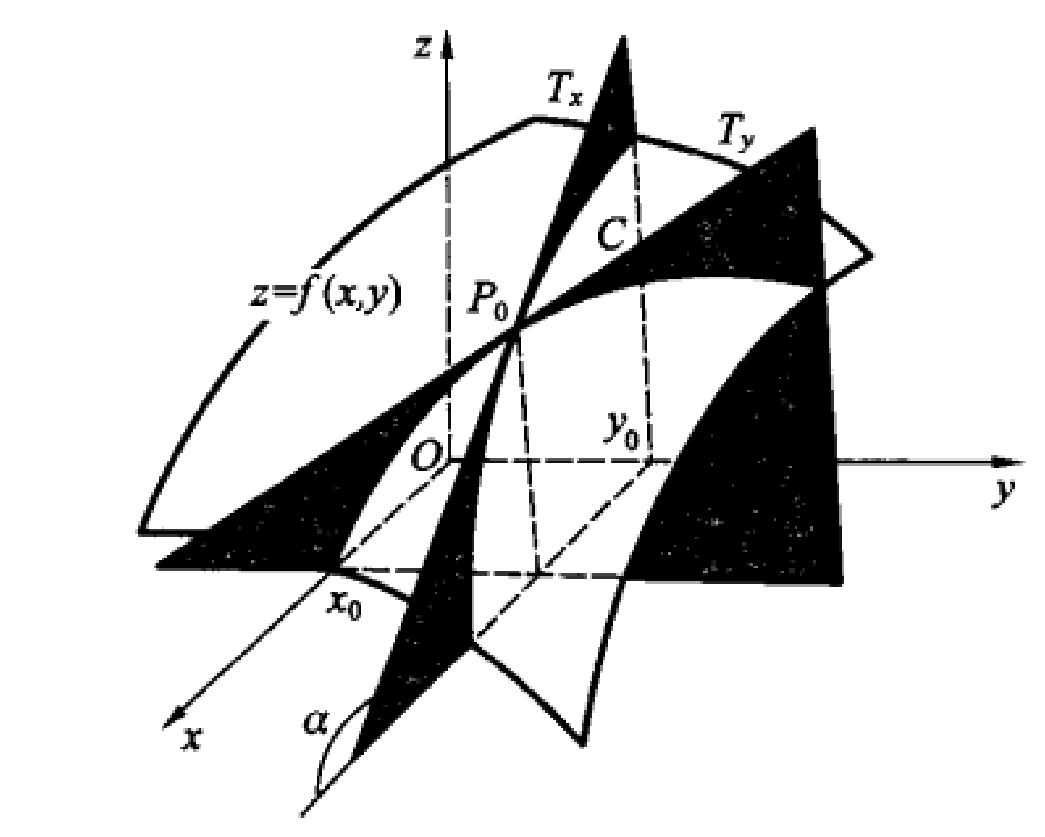
\includegraphics[width=0.5\textwidth]{work/figures/fig16-1}\caption{\relax}\label{fig:16-1}
\end{figure}

由偏导数的定义易见，求偏导数本质上归结为求一元函数的导数，只要把不相关的量视为常量即可．例如求 $f(x,y)$ 对 $x$ 的偏导数，只要把 $y$ 视为常量对 $x$ 求导即可．因此可以直接利用第四章的求导公式．

\begin{example}\label{ex:16-1-1}
设 $u=x^{y}\sin 3x$，求关于 $x$ 和 $y$ 的偏导数．
\end{example}

\begin{proof}[解]
\[
\frac{\partial u}{\partial x}=yx^{y-1}\sin 3x+3x^{y}\cos 3x,
\]
\[
\frac{\partial u}{\partial y}=x^{y}\ln x\sin 3x.
\]
\end{proof}

\begin{example}\label{ex:16-1-2}
设 $f(x,y)=\sqrt{\left|xy\right|}$，求关于 $x$ 和 $y$ 的偏导数．
\end{example}

\begin{proof}[解]
当 $x\neq 0$ 时，$f_{x}(x,y)=\dfrac{\sqrt{\left|y\right|}}{2\sqrt{\left|x\right|}}\sgn x$；

当 $y\neq 0$ 时，$f_{y}(x,y)=\dfrac{\sqrt{\left|x\right|}}{2\sqrt{\left|y\right|}}\sgn y$．

当 $x\neq 0$，$y=0$ 时，用定义求 $f_{y}$，得
\[
\lim_{\Delta y\to 0}\frac{f(x,\Delta y)-f(x,0)}{\Delta y}=\lim_{\Delta y\to 0}\frac{\sqrt{\left|x\cdot\Delta y\right|}}{\Delta y}=\infty.
\]
由此知 $f_{y}(x,0)$ 不存在 $(x\neq 0)$．同理知 $f_{x}(0,y)$ 不存在 $(y\neq 0)$．但是
\[
f_{x}(0,0)=\lim_{\Delta x\to 0}\frac{f(\Delta x,0)-f(0,0)}{\Delta x}=\lim_{\Delta x\to 0}\frac{0-0}{\Delta x}=0,
\]
\[
f_{y}(0,0)=\lim_{\Delta y\to 0}\frac{f(0,\Delta y)-f(0,0)}{\Delta y}=\lim_{\Delta y\to 0}\frac{0-0}{\Delta y}=0.
\]
综上所述：
\[
f_{x}(x,y)=\begin{cases}
\dfrac{\sqrt{\left|y\right|}}{2\sqrt{\left|x\right|}}\sgn x, & x\neq 0,\\[8pt]
\infty, & x=0,\quad y\neq 0,\\
0, & x=0,\quad y=0,
\end{cases}
\]
\[
f_{y}(x,y)=\begin{cases}
\dfrac{\sqrt{\left|x\right|}}{2\sqrt{\left|y\right|}}\sgn y, & y\neq 0,\\[8pt]
\infty, & x\neq 0,\quad y=0,\\
0, & x=0,\quad y=0.
\end{cases}
\]
\end{proof}

\begin{example}\label{ex:16-1-3}
设
\[
f(x,y)=\begin{cases}
0, & x=0\ \text{或}\ y=0,\\
1, & \text{其他}.
\end{cases}
\]
这个函数在 $(0,0)$ 点显然不连续，但
\[
f_{x}(0,0)=\lim_{\Delta x\to 0}\frac{f(\Delta x,0)-f(0,0)}{\Delta x}=\lim_{\Delta x\to 0}\frac{0-0}{\Delta x}=0.
\]
同理
\[
f_{y}(0,0)=0.
\]
也就是说，函数在原点的两个偏导数都存在，但函数在原点不连续，这在几何上是很清楚的（图~\ref{fig:16-2}）．
\end{example}

\begin{figure}[htbp]
\centering
\begin{tikzpicture}[baseline=(current bounding box.center)]
  \def\hz{1.7}
  \def\ax{1.5}
  \def\ay{2.6}
  % screen vectors: +x -> (-0.78,-0.56), +y -> (1,0), +z -> (0,1)
  \fill[gray!10,draw,thick] (0,\hz) -- ({-\ax*0.78},{\hz-\ax*0.56}) -- ({-\ax*0.78+\ay},{\hz-\ax*0.56}) -- (\ay,\hz) -- cycle;
  \fill[gray!10,draw,thick] (0,\hz) -- ({-\ax*0.78},{\hz-\ax*0.56}) -- ({-\ax*0.78-\ay},{\hz-\ax*0.56}) -- (-\ay,\hz) -- cycle;
  \fill[gray!10,draw,thick] (0,\hz) -- ({\ax*0.78},{\hz+\ax*0.56}) -- ({\ax*0.78+\ay},{\hz+\ax*0.56}) -- (\ay,\hz) -- cycle;
  \fill[gray!10,draw,thick] (0,\hz) -- ({\ax*0.78},{\hz+\ax*0.56}) -- ({\ax*0.78-\ay},{\hz+\ax*0.56}) -- (-\ay,\hz) -- cycle;
  \draw[{-Latex}] (0,0) -- (-2,-1.45) node[below left] {$x$};
  \draw[{-Latex}] (0,0) -- (3.6,0) node[below left] {$y$};
  \draw[{-Latex}] (0,-0.9) -- (0,3.2) node[left] {$z$};
  \node[below left] at (0,0) {$O$};
  \node[left] at (0,\hz) {$1$};
\end{tikzpicture}\caption{\relax}\label{fig:16-2}
\end{figure}

例~\ref{ex:16-1-3} 表明，二元函数 $f(x,y)$ 在某点的两个偏导数存在，并不能推出函数在该点连续，这与一元函数 $f(x)$ 在一点可导就连续是不同的．事实上，二元函数在几何上是曲面，而函数在一点 $(x_{0},y_{0})$ 的两个偏导数存在只说明曲面上过 $(x_{0},y_{0})$ 点的两条特殊的曲线在该点有切线，它当然不能完全反映曲面在该点的性质（如连续性）．为此，下面引入全微分的概念．

\subsection{全微分}

回忆一元函数的微分，它具有两大重要特性：微分是自变量的改变量的线性函数；微分与函数的改变量之差是比自变量的改变量更高阶的无穷小量．也就是说微分是函数改变量的线性主要部分．把它推广到二元函数，我们引出如下定义．

\begin{definition}\label{def:16-2}
设函数 $z=f(x,y)$ 在 $P_{0}(x_{0},y_{0})$ 点的某邻域有定义．若函数 $f$ 在 $P_{0}$ 点的全改变量 $\Delta z$ 可表为
\begin{equation}
\begin{aligned}
\Delta z&=f(x_{0}+\Delta x,y_{0}+\Delta y)-f(x_{0},y_{0})\\
&=A\Delta x+B\Delta y+o(\rho),
\end{aligned}
\tag{1}
\end{equation}
其中 $A$，$B$ 是与 $\Delta x$，$\Delta y$ 无关（可与 $P_{0}$ 有关）的常数，$\rho=\sqrt{(\Delta x)^{2}+(\Delta y)^{2}}$，$o(\rho)$ 是比 $\rho$ 更高阶的无穷小量，则称函数在 $P_{0}$ 点可微．并称 $A\Delta x+B\Delta y$ 为函数 $f$ 在点 $P_{0}$ 的全微分，记为
\[
\dd z\mid_{P_{0}}=A\Delta x+B\Delta y.
\]
\end{definition}

从定义可见，二元函数的全微分同一元函数的微分一样，仍然具有两大特性，即二元函数的全微分是自变量的改变量的线性函数；微分与函数的全改变量之差是比 $\rho$ 更高阶的无穷小量．综合起来说就是：二元函数的全微分是函数全改变量的线性主要部分．

下面看看二元函数 $z=f(x,y)$ 在 $(x_{0},y_{0})$ 可微的几何意义．先回忆一元函数的情形．我们知道，$y=f(x)$ 在 $x_{0}$ 可微，是说函数 $y=f(x)$ 在 $x_{0}$ 的改变量 $\Delta y=f(x_{0}+\Delta x)-f(x_{0})$ 有线性主要部分 $A\Delta x=f^{\prime}(x_{0})\Delta x$，即
\begin{equation}
\Delta y=A\Delta x+o(\Delta x)=f^{\prime}(x_{0})\Delta x+o(\Delta x).
\tag{2}
\end{equation}
记 $x=x_{0}+\Delta x$，即 $\Delta x=x-x_{0}$，则（2）可写成
\begin{equation}
f(x)-f(x_{0})=f^{\prime}(x_{0})(x-x_{0})+o(x-x_{0}),
\tag{3}
\end{equation}
或
\begin{equation}
f(x)=f(x_{0})+f^{\prime}(x_{0})(x-x_{0})+o(x-x_{0}).
\tag{4}
\end{equation}
注意 $y=f(x_{0})+f^{\prime}(x_{0})(x-x_{0})$ 是曲线 $y=f(x)$ 在 $x_{0}$ 的切线，故（3）说明，函数 $f(x)$ 在 $x_{0}$ 可微，是指曲线 $y=f(x)$ 在 $x_{0}$ 有切线存在，且曲线 $y=f(x)$ 在 $x_{0}$ 附近可用直线（切线）来逼近，其误差当 $x\to x_{0}$ 时是 $x-x_{0}$ 的高阶无穷小量（见图~\ref{fig:16-3}）．

\begin{figure}[htbp]
\centering
\begin{tikzpicture}[scale=0.85,baseline=(current bounding box.center)]
  \draw[{-Latex}] (0,0) -- (4.8,0) node[below left] {$x$};
  \draw[{-Latex}] (0.7,-0.5) -- (0.7,3.3) node[left] {$y$};
  \node[below left] at (0.7,0) {$O$};
  \coordinate (P) at (1.6,1.05);
  \coordinate (Q) at (3.7,2.65);
  \coordinate (Q') at (3.7,1.85);
  \draw[thick] (0.35,0.55) .. controls (1.2,0.9) and (2.4,1.6) .. (4.3,3.2);
  \draw[thick] (0.85,0.73) -- (4.35,2.23);
  \fill (P) circle (1.3pt) node[above left] {$P$};
  \fill (Q) circle (1.3pt) node[above right] {$Q$};
  \fill (Q') circle (1.3pt) node[right] {$Q^{\prime}$};
  \draw[dashed] (P) -- (1.6,0) node[below] {$x_{0}$};
  \draw[dashed] (Q) -- (3.7,0) node[below] {$x_{0}+\Delta x$};
  \draw[dashed] (P) -- (3.7,1.05);
  \draw[latex-latex] (3.55,1.05) -- (3.55,1.85) node[left] {$\dd y$};
  \draw[latex-latex] (3.85,1.05) -- (3.85,2.65) node[right] {$\Delta y$};
\end{tikzpicture}\caption{\relax}\label{fig:16-3}
\end{figure}

对于二元函数 $z=f(x,y)$，记 $x=x_{0}+\Delta x$，$y=y_{0}+\Delta y$，即 $\Delta x=x-x_{0}$，$\Delta y=y-y_{0}$，则公式（1）可写成
\begin{equation}
f(x,y)-f(x_{0},y_{0})=A(x-x_{0})+B(y-y_{0})+o(\rho),
\tag{5}
\end{equation}
或
\begin{equation}
f(x,y)=f(x_{0},y_{0})+A(x-x_{0})+B(y-y_{0})+o(\rho),
\tag{6}
\end{equation}
其中 $\rho=\sqrt{(x-x_{0})^{2}+(y-y_{0})^{2}}$．（6）式右边的前一部分是 $x$，$y$ 的线性函数，即
\begin{equation}
z=f(x_{0},y_{0})+A(x-x_{0})+B(y-y_{0}).
\tag{7}
\end{equation}
由解析几何的知识可知，它是一空间平面方程，且过 $(x_{0},y_{0},f(x_{0},y_{0}))$．（6）式说，这个平面与曲面 $z=f(x,y)$ 在 $(x_{0},y_{0})$ 附近之差，当 $\rho\to 0$ 时是较 $\rho$ 更高阶的无穷小量．也就是说，曲面 $z=f(x,y)$ 在 $(x_{0},y_{0},f(x_{0},y_{0}))$ 附近，与一个平面十分密切．这平面当然不是别的，正是曲面过 $(x_{0},y_{0},f(x_{0},y_{0}))$ 的切平面．可以说，函数 $f(x,y)$ 在 $(x_{0},y_{0})$ 可微，其几何意义是曲面 $z=f(x,y)$ 在 $(x_{0},y_{0},f(x_{0},y_{0}))$ 有切平面存在，全微分就是线性函数在 $(x_{0},y_{0})$ 的改变量（见图~\ref{fig:16-4}）．由此可见，全微分刻画的是函数 $f(x,y)$ 在 $(x_{0},y_{0})$ 附近的全面变化，而不像偏导数那样，只描写函数在两个特殊方向的变化．下面的定理也进一步说明这一点．

\begin{figure}[htbp]
\centering
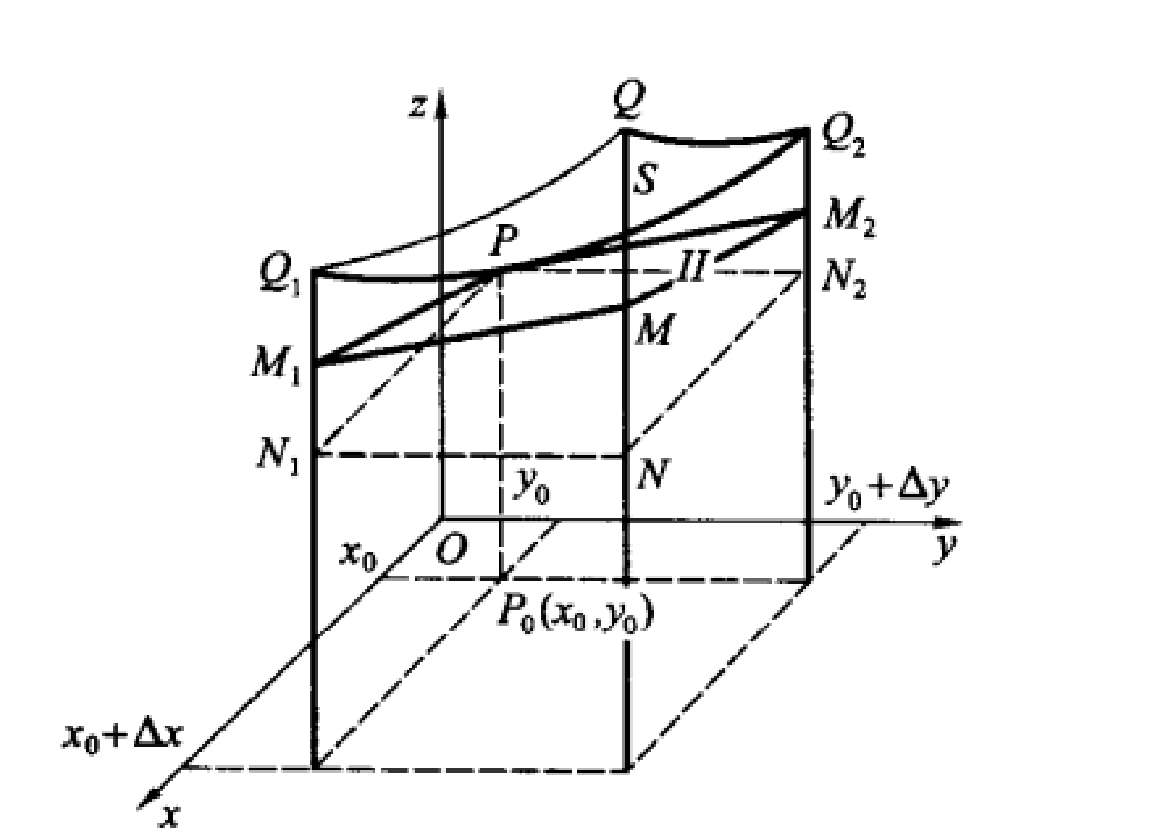
\includegraphics[width=0.55\textwidth]{work/figures/fig16-4}\caption{\relax}\label{fig:16-4}
\end{figure}

\begin{theorem}\label{thm:16-1}
若 $f(x,y)$ 在点 $P_{0}(x_{0},y_{0})$ 可微，则 $f(x,y)$ 在点 $P_{0}$ 连续．
\end{theorem}

\begin{proof}
由可微性知
\[
f(x,y)=f(x_{0},y_{0})+A(x-x_{0})+B(y-y_{0})+o(\rho),
\]
其中
\[
\rho=\sqrt{(x-x_{0})^{2}+(y-y_{0})^{2}}.
\]
令 $x\to x_{0}$，$y\to y_{0}$ 取极限，有
\[
\lim_{\substack{x\to x_{0}\\ y\to y_{0}}}f(x,y)=f(x_{0},y_{0}).
\]
这就证明了 $f(x,y)$ 在点 $P_{0}(x_{0},y_{0})$ 连续．定理~\ref{thm:16-1} 证完．
\end{proof}

\subsection{全微分与偏导数的关系}

若 $f(x,y)$ 在 $(x_{0},y_{0})$ 可微，则有
\[
\begin{aligned}
&f(x_{0}+\Delta x,y_{0}+\Delta y)-f(x_{0},y_{0})\\
={}&A\Delta x+B\Delta y+o\left(\sqrt{(\Delta x)^{2}+(\Delta y)^{2}}\right),
\end{aligned}
\]
特别地，令 $\Delta y=0$ 得
\[
f(x_{0}+\Delta x,y_{0})-f(x_{0},y_{0})=A\Delta x+o(\left|\Delta x\right|).
\]
因此
\[
\frac{f(x_{0}+\Delta x,y_{0})-f(x_{0},y_{0})}{\Delta x}=A+\frac{o(\left|\Delta x\right|)}{\Delta x}.
\]
令 $\Delta x\to 0$ 取极限，知左边的极限存在，且等于 $A$，即 $f_{x}(x_{0},y_{0})$ 存在，且
\[
A=f_{x}(x_{0},y_{0}).
\]
同理可得 $f_{y}(x_{0},y_{0})$ 存在，且
\[
B=f_{y}(x_{0},y_{0}).
\]
这样我们便证明了下面的定理．

\begin{theorem}\label{thm:16-2}
若 $z=f(x,y)$ 在点 $P_{0}(x_{0},y_{0})$ 可微，则 $f_{x}(x_{0},y_{0})$ 和 $f_{y}(x_{0},y_{0})$ 都存在，且 $f(x,y)$ 在点 $P_{0}$ 的全微分等于
\[
f_{x}(x_{0},y_{0})\Delta x+f_{y}(x_{0},y_{0})\Delta y.
\]
\end{theorem}

约定自变量的改变量等于自变量的微分，即
\[
\Delta x=\dd x,\quad \Delta y=\dd y,
\]
则 $f$ 在点 $P_{0}$ 的全微分又可写为
\[
\dd z\mid_{P_{0}}=f_{x}(x_{0},y_{0})\dd x+f_{y}(x_{0},y_{0})\dd y.
\]
若 $z=f(x,y)$ 在某区域 $G$ 上每点可微，则
\[
\dd z=f_{x}(x,y)\dd x+f_{y}(x,y)\dd y.
\]
值得指出的是，$\dd z$ 是 $x$，$y$，$\dd x$，$\dd y$ 的四元函数，对固定的 $x$，$y$，它是 $\dd x$ 与 $\dd y$ 的二元线性函数．

类似地可以定义 $n$ 元函数 $u=f(x_{1},x_{2},\cdots,x_{n})$ 的全微分，相应的公式为
\[
\dd u=\frac{\partial u}{\partial x_{1}}\dd x_{1}+\frac{\partial u}{\partial x_{2}}\dd x_{2}+\cdots+\frac{\partial u}{\partial x_{n}}\dd x_{n}.
\]
我们已经知道函数在一点的两个偏导数存在并不能推出函数在该点连续，因此，更不能推出在该点可微．不过我们有下面的定理．

\begin{theorem}\label{thm:16-3}
若函数 $u=f(x,y)$ 在 $P_{0}(x_{0},y_{0})$ 点的某邻域 $O(P_{0})$ 内存在偏导数，且 $f_{x}(x,y)$，$f_{y}(x,y)$ 在 $P_{0}$ 点连续，则 $f(x,y)$ 在 $P_{0}$ 点可微．
\end{theorem}

\begin{proof}
设 $\left|\Delta x\right|$，$\left|\Delta y\right|$ 充分小使得 $(x_{0}+\Delta x,y_{0}+\Delta y)\in O(P_{0})$．将 $\Delta f(x_{0},y_{0})$ 表为
\[
\begin{aligned}
\Delta f(x_{0},y_{0})&=f(x_{0}+\Delta x,y_{0}+\Delta y)-f(x_{0},y_{0})\\
&=\left[f(x_{0}+\Delta x,y_{0}+\Delta y)-f(x_{0}+\Delta x,y_{0})\right]\\
&\quad+\left[f(x_{0}+\Delta x,y_{0})-f(x_{0},y_{0})\right].
\end{aligned}
\]
由一元函数的微分中值定理，存在 $\theta_{1},\theta_{2}\in(0,1)$，使得
\[
\Delta f(x_{0},y_{0})=f_{y}(x_{0}+\Delta x,y_{0}+\theta_{1}\Delta y)\Delta y+f_{x}(x_{0}+\theta_{2}\Delta x,y_{0})\Delta x.
\]
由 $f_{x}$ 和 $f_{y}$ 在 $(x_{0},y_{0})$ 点连续，知
\[
\lim_{\substack{\Delta x\to 0\\ \Delta y\to 0}}f_{x}(x_{0}+\theta_{2}\Delta x,y_{0})=f_{x}(x_{0},y_{0}),
\]
\[
\lim_{\substack{\Delta x\to 0\\ \Delta y\to 0}}f_{y}(x_{0}+\Delta x,y_{0}+\theta_{1}\Delta y)=f_{y}(x_{0},y_{0}),
\]
从而有
\[
\begin{aligned}
f_{x}(x_{0}+\theta_{2}\Delta x,y_{0})&=f_{x}(x_{0},y_{0})+\alpha,\\
f_{y}(x_{0}+\Delta x,y_{0}+\theta_{1}\Delta y)&=f_{y}(x_{0},y_{0})+\beta,
\end{aligned}
\]
其中当 $\Delta x\to 0$ 且 $\Delta y\to 0$ 即 $\rho\to 0$ 时，$\alpha\to 0$，$\beta\to 0$，故
\[
\Delta f(x_{0},y_{0})=f_{x}(x_{0},y_{0})\Delta x+f_{y}(x_{0},y_{0})\Delta y+\alpha\Delta x+\beta\Delta y;
\]
而
\[
\left|\frac{\alpha\Delta x+\beta\Delta y}{\sqrt{(\Delta x)^{2}+(\Delta y)^{2}}}\right|\leqslant\left|\alpha\right|+\left|\beta\right|\to 0\quad(\rho\to 0),
\]
即 $\alpha\Delta x+\beta\Delta y=o(\rho)$．这就证明了 $f(x,y)$ 在 $P_{0}$ 可微．定理~\ref{thm:16-3} 证完．
\end{proof}

从定理证明可知，全微分定义中的（1）式等价于
\[
\Delta f(x_{0},y_{0})=A\Delta x+B\Delta y+\alpha\Delta x+\beta\Delta y,
\]
其中当 $\rho\to 0$ 时，$\alpha\to 0$，$\beta\to 0$．这个表达式有时用起来更为方便．

\begin{example}\label{ex:16-1-4}
设 $u=x^{2}y+\mathrm{e}^{xy}$，求全微分 $\dd u$．
\end{example}

\begin{proof}[解]
\[
\frac{\partial u}{\partial x}=2xy+y\mathrm{e}^{xy},
\]
\[
\frac{\partial u}{\partial y}=x^{2}+x\mathrm{e}^{xy},
\]
$\dfrac{\partial u}{\partial x}$，$\dfrac{\partial u}{\partial y}$ 都在全平面上连续，故函数在全平面上可微，且
\[
\dd u=(2xy+y\mathrm{e}^{xy})\dd x+(x^{2}+x\mathrm{e}^{xy})\dd y.
\]
\end{proof}

\begin{example}\label{ex:16-1-5}
考察函数
\[
f(x,y)=\begin{cases}
\dfrac{xy}{\sqrt{x^{2}+y^{2}}}, & x^{2}+y^{2}\neq 0,\\
0, & x^{2}+y^{2}=0
\end{cases}
\]
在原点的可微性．
\end{example}

\begin{proof}[解]
由偏导数的定义
\[
f_{x}(0,0)=\lim_{\Delta x\to 0}\frac{f(\Delta x,0)-f(0,0)}{\Delta x}=0,
\]
同理可得 $f_{y}(0,0)=0$．若函数 $f$ 在原点可微，则按可微的定义，应有
\[
\begin{aligned}
&f(\Delta x,\Delta y)-f(0,0)-\left[f_{x}(0,0)\Delta x+f_{y}(0,0)\Delta y\right]\\
={}&\frac{\Delta x\Delta y}{\sqrt{(\Delta x)^{2}+(\Delta y)^{2}}}
\end{aligned}
\]
是比 $\rho$ 更高阶的无穷小量．为此考察极限
\[
\lim_{\substack{\Delta x\to 0\\ \Delta y\to 0}}\frac{\dfrac{\Delta x\Delta y}{\sqrt{(\Delta x)^{2}+(\Delta y)^{2}}}}{\rho}=\lim_{\substack{\Delta x\to 0\\ \Delta y\to 0}}\frac{\Delta x\Delta y}{(\Delta x)^{2}+(\Delta y)^{2}}.
\]
由第十五章 §2 例 5 知，上述极限不存在，故 $f$ 在原点不可微．
\end{proof}

根据定理~\ref{thm:16-3} 我们还可知，上例中的偏导数 $f_{x}(x,y)$ 和 $f_{y}(x,y)$ 在原点必不连续．这一点也可以通过计算直接证明．事实上，
\[
f_{x}(x,y)=\begin{cases}
\dfrac{y^{3}}{\left(x^{2}+y^{2}\right)^{\frac{3}{2}}}, & x^{2}+y^{2}\neq 0,\\[6pt]
0, & x^{2}+y^{2}=0,
\end{cases}
\]
而
\[
\lim_{\substack{y=kx\\ x\to 0}}f_{x}(x,y)=\lim_{x\to 0}f_{x}(x,kx)=\lim_{x\to 0}\frac{k^{3}x^{3}}{(1+k^{2})^{\frac{3}{2}}x^{3}}=\frac{k^{3}}{(1+k^{3})^{\frac{3}{2}}}.
\]
因此 $\lim\limits_{\substack{x\to 0\\ y\to 0}}f_{x}(x,y)$ 不存在，这就证明了 $f_{x}(x,y)$ 在 $(0,0)$ 点不连续．由 $f(x,y)$ 关于 $x$、$y$ 的对称性知，$f_{y}(x,y)$ 在 $(0,0)$ 点也不连续．

请读者思考，若 $f_{x}(x,y)$ 和 $f_{y}(x,y)$ 都在 $(x_{0},y_{0})$ 点不连续，是否能推知 $f(x,y)$ 在 $(x_{0},y_{0})$ 点不可微？

最后我们把函数在某点连续、存在偏导数及可微之间的关系简单地总结如下：
\[
\text{两个偏导数都连续}\Rightarrow\text{可微}\Rightarrow\text{连续}.
\]
逆过来均不成立．

用全微分可以近似计算函数值．

\begin{example}\label{ex:16-1-6}
求 $1.08^{3.96}$ 的近似值．
\end{example}

\begin{proof}[解]
设 $f(x,y)=x^{y}$，令 $x_{0}=1$，$y_{0}=4$，$\Delta x=0.08$，$\Delta y=-0.04$，则
\[
\begin{aligned}
1.08^{3.96}&=f(x_{0}+\Delta x,y_{0}+\Delta y)\\
&\approx f(1,4)+f_{x}(1,4)\Delta x+f_{y}(1,4)\Delta y\\
&=1+4\times 0.08+(-0.04)\ln 1\\
&=1+0.32=1.32.
\end{aligned}
\]
\end{proof}

\subsection{高阶偏导数与高阶全微分}

我们先考虑二元函数 $u=f(x,y)$ 的高阶偏导数．一般说来偏导数 $f_{x}(x,y)$，$f_{y}(x,y)$ 仍是 $x$、$y$ 的函数．如果它们关于 $x$、$y$ 的偏导数存在，则称 $f_{x}(x,y)$ 和 $f_{y}(x,y)$ 关于 $x$、$y$ 的偏导数为 $f(x,y)$ 的二阶偏导数．按排列组合，二元函数的二阶偏导数有四个，分别记为
\[
\frac{\partial f_{x}}{\partial x}=\frac{\partial^{2}f}{\partial x^{2}}=f_{xx}\quad\text{或}\quad\frac{\partial^{2}u}{\partial x^{2}},
\]
\[
\frac{\partial f_{x}}{\partial y}=\frac{\partial^{2}f}{\partial x\partial y}=f_{xy}\quad\text{或}\quad\frac{\partial^{2}u}{\partial x\partial y},
\]
\[
\frac{\partial f_{y}}{\partial x}=\frac{\partial^{2}f}{\partial y\partial x}=f_{yx}\quad\text{或}\quad\frac{\partial^{2}u}{\partial y\partial x},
\]
\[
\frac{\partial f_{y}}{\partial y}=\frac{\partial^{2}f}{\partial y^{2}}=f_{yy}\quad\text{或}\quad\frac{\partial^{2}u}{\partial y^{2}}.
\]
其中 $\dfrac{\partial^{2}f}{\partial x\partial y}$ 和 $\dfrac{\partial^{2}f}{\partial y\partial x}$ 称为二阶混合偏导数．

类似地可定义三阶偏导数，如
\[
\frac{\partial}{\partial x}\left(\frac{\partial^{2}f}{\partial x^{2}}\right)=\frac{\partial^{3}f}{\partial x^{3}},
\]
\[
\frac{\partial}{\partial y}\left(\frac{\partial^{2}f}{\partial x^{2}}\right)=\frac{\partial^{3}f}{\partial x^{2}\partial y},
\]
\[
\frac{\partial}{\partial x}\left(\frac{\partial^{2}f}{\partial x\partial y}\right)=\frac{\partial^{3}f}{\partial x\partial y\partial x},
\]
等等．

\begin{example}\label{ex:16-1-7}
设 $u=x^{4}+y^{4}-4x^{3}y^{2}$，求所有二阶偏导数．
\end{example}

\begin{proof}[解]
$\dfrac{\partial u}{\partial x}=4x^{3}-12x^{2}y^{2}$，$\dfrac{\partial u}{\partial y}=4y^{3}-8x^{3}y$，
\[
\frac{\partial^{2}u}{\partial x^{2}}=12x^{2}-24xy^{2},\quad\frac{\partial^{2}u}{\partial x\partial y}=-24x^{2}y,
\]
\[
\frac{\partial^{2}u}{\partial y\partial x}=-24x^{2}y,\quad\frac{\partial^{2}u}{\partial y^{2}}=12y^{2}-8x^{3}.
\]
\end{proof}

上例中的两个混合偏导数 $\dfrac{\partial^{2}u}{\partial x\partial y}$ 和 $\dfrac{\partial^{2}u}{\partial y\partial x}$ 恰好相等，也就是说这个函数的二阶混合偏导数与对变量 $x$，$y$ 的求偏导顺序无关．我们自然要问，是否对所有的二元函数，只要两个二阶混合偏导数存在，都有 $\dfrac{\partial^{2}u}{\partial x\partial y}=\dfrac{\partial^{2}u}{\partial y\partial x}$ 呢？请看下面的例子．

\begin{example}\label{ex:16-1-8}
设
\[
f(x,y)=\begin{cases}
xy\dfrac{x^{2}-y^{2}}{x^{2}+y^{2}}, & x^{2}+y^{2}\neq 0,\\
0, & x^{2}+y^{2}=0,
\end{cases}
\]
证明 $f_{xy}(0,0)\neq f_{yx}(0,0)$．
\end{example}

\begin{proof}
由于
\[
f_{x}(x,y)=\begin{cases}
y\left(\dfrac{x^{2}-y^{2}}{x^{2}+y^{2}}+\dfrac{4x^{2}y^{2}}{(x^{2}+y^{2})^{2}}\right), & x^{2}+y^{2}\neq 0,\\
0, & x^{2}+y^{2}=0,
\end{cases}
\]
\[
f_{y}(x,y)=\begin{cases}
x\left(\dfrac{x^{2}-y^{2}}{x^{2}+y^{2}}-\dfrac{4x^{2}y^{2}}{(x^{2}+y^{2})^{2}}\right), & x^{2}+y^{2}\neq 0,\\
0, & x^{2}+y^{2}=0,
\end{cases}
\]
因此
\[
f_{xy}(0,0)=\lim_{y\to 0}\frac{f_{x}(0,y)-f_{x}(0,0)}{y}=\lim_{y\to 0}\frac{-y}{y}=-1,
\]
\[
f_{yx}(0,0)=\lim_{x\to 0}\frac{f_{y}(x,0)-f_{y}(0,0)}{x}=\lim_{x\to 0}\frac{x}{x}=1.
\]
\end{proof}

这个例子回答了上面提出的问题．两个混合偏导数都存在并不能保证它们相等．那么在什么条件下才能保证两者相等呢？下面给出一个相等的充分条件．

\begin{theorem}\label{thm:16-4}
若 $f_{xy}(x,y)$ 和 $f_{yx}(x,y)$ 在点 $(x,y)$ 都连续，则
\[
f_{xy}(x,y)=f_{yx}(x,y).
\]
\end{theorem}

\begin{proof}
先将 $f_{xy}(x,y)$ 和 $f_{yx}(x,y)$ 表成极限形式．因为
\[
f_{x}(x,y)=\lim_{\Delta x\to 0}\frac{f(x+\Delta x,y)-f(x,y)}{\Delta x},
\]
所以
\[
\begin{aligned}
&f_{xy}(x,y)\\
={}&\lim_{\Delta y\to 0}\frac{f_{x}(x,y+\Delta y)-f_{x}(x,y)}{\Delta y}\\
={}&\lim_{\Delta y\to 0}\frac{1}{\Delta y}\left[\lim_{\Delta x\to 0}\left(\frac{f(x+\Delta x,y+\Delta y)-f(x,y+\Delta y)}{\Delta x}-\frac{f(x+\Delta x,y)-f(x,y)}{\Delta x}\right)\right]\\
={}&\lim_{\Delta y\to 0}\lim_{\Delta x\to 0}\frac{f(x+\Delta x,y+\Delta y)-f(x,y+\Delta y)-f(x+\Delta x,y)+f(x,y)}{\Delta x\Delta y}.
\end{aligned}
\]
同理
\[
f_{yx}(x,y)=\lim_{\Delta x\to 0}\lim_{\Delta y\to 0}\frac{f(x+\Delta x,y+\Delta y)-f(x+\Delta x,y)-f(x,y+\Delta y)+f(x,y)}{\Delta x\Delta y}.
\]
我们发现，两个取极限的公式，其分子是相等的．因此，记
\[
\begin{aligned}
F(\Delta x,\Delta y)&=\left[f(x+\Delta x,y+\Delta y)-f(x+\Delta x,y)\right]-\\
&\quad\left[f(x,y+\Delta y)-f(x,y)\right],
\end{aligned}
\]
如果令
\[
\varphi(x)=f(x,y+\Delta y)-f(x,y),
\]
则
\[
F(\Delta x,\Delta y)=\varphi(x+\Delta x)-\varphi(x).
\]
由于 $f_{xy}(x,y)$ 在 $(x,y)$ 点连续，知 $f_{x}(x,y)$ 在 $(x,y)$ 点的某邻域存在，因此 $\varphi(x)$ 在 $x$ 点的某邻域可导．根据一元函数的微分中值定理，当 $\left|\Delta x\right|$ 充分小时，存在 $\theta_{1}\in(0,1)$，使得
\[
\begin{aligned}
F(\Delta x,\Delta y)&=\varphi^{\prime}(x+\theta_{1}\Delta x)\Delta x\\
&=\left[f_{x}(x+\theta_{1}\Delta x,y+\Delta y)-f_{x}(x+\theta_{1}\Delta x,y)\right]\Delta x.
\end{aligned}
\]
对 $y$ 再用一次微分中值定理，知存在 $\theta_{2}\in(0,1)$，使得
\begin{equation}
F(\Delta x,\Delta y)=f_{xy}(x+\theta_{1}\Delta x,y+\theta_{2}\Delta y)\Delta x\Delta y.
\tag{8}
\end{equation}
类似地，如果令
\[
\psi(y)=f(x+\Delta x,y)-f(x,y),
\]
则
\[
F(\Delta x,\Delta y)=\psi(y+\Delta y)-\psi(y).
\]
用微分中值定理，存在 $\theta_{3}\in(0,1)$，使得
\[
\begin{aligned}
F(\Delta x,\Delta y)&=\psi^{\prime}(y+\theta_{3}\Delta y)\Delta y\\
&=\left[f_{y}(x+\Delta x,y+\theta_{3}\Delta y)-f_{y}(x,y+\theta_{3}\Delta y)\right]\Delta y.
\end{aligned}
\]
再对 $x$ 用一次微分中值定理，知存在 $\theta_{4}\in(0,1)$，使得
\begin{equation}
F(\Delta x,\Delta y)=f_{yx}(x+\theta_{4}\Delta x,y+\theta_{3}\Delta y)\Delta x\Delta y.
\tag{9}
\end{equation}
比较（8）与（9），便得
\[
f_{xy}(x+\theta_{1}\Delta x,y+\theta_{2}\Delta y)=f_{yx}(x+\theta_{4}\Delta x,y+\theta_{3}\Delta y),
\]
其中 $\theta_{1}$，$\theta_{2}$，$\theta_{3}$，$\theta_{4}\in(0,1)$．令 $\Delta x\to 0$，$\Delta y\to 0$ 取极限，由两个混合偏导数都连续，知
\[
f_{xy}(x,y)=f_{yx}(x,y),
\]
定理~\ref{thm:16-4} 证完．
\end{proof}

这个定理可以推广到 $n$ 阶偏导数的情形，即若函数 $f$ 具有直到 $n$ 阶的连续偏导数，则求偏导数与变量的顺序无关．这样，二元函数 $f(x,y)$ 的 $n$ 阶偏导数就可简单地表示为
\[
\frac{\partial^{n}f}{\partial x^{k}\partial y^{n-k}},\quad k=0,1,2,\cdots,n.
\]
有了高阶偏导数，我们来定义高阶全微分．函数 $u=f(x,y)$ 的一阶全微分
\[
\dd u=f_{x}(x,y)\dd x+f_{y}(x,y)\dd y
\]
仍是 $x$，$y$ 的函数．若作为 $x$，$y$ 的函数，它是可微的，则它的全微分称为 $f(x,y)$ 的二阶全微分，这就是
\[
\begin{aligned}
\dd^{2}u&=\dd(\dd u)=\dd\left[f_{x}(x,y)\dd x\right]+\dd\left[f_{y}(x,y)\dd y\right]\\
&=\left[f_{xx}(x,y)\dd x+f_{xy}(x,y)\dd y\right]\dd x+\left[f_{yx}(x,y)\dd x+f_{yy}(x,y)\dd y\right]\dd y\\
&=f_{xx}(x,y)\dd x^{2}+\left[f_{xy}(x,y)+f_{yx}(x,y)\right]\dd x\dd y+f_{yy}(x,y)\dd y^{2}.
\end{aligned}
\]
要特别强调的是二阶全微分是一阶全微分作为 $x$，$y$ 的函数的全微分．一阶全微分依赖于四个独立的变量 $x$，$y$，$\dd x$ 和 $\dd y$，其中 $\dd x$ 和 $\dd y$ 是自变量的微分，是与 $x$，$y$ 无关的．因此求二阶全微分时，变量只有 $x$ 和 $y$，而
\[
\dd(\dd x)=\dd(\dd y)=0.
\]
当混合偏导数连续时，有
\[
\begin{aligned}
\dd^{2}u&=f_{xx}(x,y)\dd x^{2}+2f_{xy}(x,y)\dd x\dd y+f_{yy}(x,y)\dd y^{2}\\
&=\sum_{k=0}^{2}\mathrm{C}_{2}^{k}\frac{\partial^{2}f(x,y)}{\partial x^{2-k}\partial y^{k}}\dd x^{2-k}\dd y^{k}.
\end{aligned}
\]
为书写方便，我们把 $\dfrac{\partial}{\partial x}$ 和 $\dfrac{\partial}{\partial y}$ 视为算子，规定
\[
\left(\frac{\partial}{\partial x}\right)^{i}\left(\frac{\partial}{\partial y}\right)^{j}=\frac{\partial^{i+j}}{\partial x^{i}\partial y^{j}},
\]
\[
\frac{\partial^{n}}{\partial x^{n-k}\partial y^{k}}(af(x,y))=a\frac{\partial^{n}f(x,y)}{\partial x^{n-k}\partial y^{k}},\quad a\ \text{是常数},
\]
\[
\left(\frac{\partial^{n}}{\partial x^{n-k}\partial y^{k}}+\frac{\partial^{m}}{\partial x^{m-l}\partial y^{l}}\right)f(x,y)=\frac{\partial^{n}f(x,y)}{\partial x^{n-k}\partial y^{k}}+\frac{\partial^{m}f(x,y)}{\partial x^{m-l}\partial y^{l}},
\]
\[
k=0,1,2,\cdots,n,\quad l=0,1,2,\cdots,m.
\]
这时
\[
\dd^{2}u=\left(\frac{\partial}{\partial x}\dd x+\frac{\partial}{\partial y}\dd y\right)^{2}f(x,y).
\]
类似地可定义 $n$ 阶全微分为 $\dd^{n}u=\dd(\dd^{n-1}u)$．用归纳法可以证明，当 $n$ 阶偏导数连续时，有
\[
\begin{aligned}
\dd^{n}u&=\sum_{k=0}^{n}\mathrm{C}_{n}^{k}\frac{\partial^{n}f(x,y)}{\partial x^{n-k}\partial y^{k}}\dd x^{n-k}\dd y^{k}\\
&=\left(\frac{\partial}{\partial x}\dd x+\frac{\partial}{\partial y}\dd y\right)^{n}f(x,y).
\end{aligned}
\]

\begin{xiti}
\item 求下列函数的偏导数：
\begin{ziti}
\item $u=x^{2}\ln(x^{2}+y^{2})$；
\item $u=(x+y)\cos(xy)$；
\item $u=\arctan\dfrac{y}{x}$；
\item $u=xy+\dfrac{x}{y}$；
\item $u=xy\,\mathrm{e}^{\sin(xy)}$；
\item $u=x^{y}+y^{x}$．
\end{ziti}
\item 设
\[
f(x,y)=\begin{cases}
y\sin\dfrac{1}{x^{2}+y^{2}}, & x^{2}+y^{2}\neq 0,\\
0, & x^{2}+y^{2}=0.
\end{cases}
\]
考察函数在 $(0,0)$ 点的偏导数．
\item 证明函数 $u=\sqrt{x^{2}+y^{2}}$ 在 $(0,0)$ 点连续但偏导数不存在．
\item 求下列函数的全微分：
\begin{ziti}
\item $u=\sqrt{x^{2}+y^{2}+z^{2}}$；
\item $u=x\mathrm{e}^{yz}+\mathrm{e}^{-x}+y$．
\end{ziti}
\item 求下列函数在给定点的全微分：
\begin{ziti}
\item $u=\dfrac{x}{\sqrt{x^{2}+y^{2}}}$ 在点 $(1,0)$ 和 $(0,1)$；
\item $u=\ln(x+y^{2})$ 在点 $(0,1)$ 和 $(1,1)$；
\item $u=\sqrt[z]{\dfrac{x}{y}}$ 在点 $(1,1,1)$；
\item $u=x+(y-1)\arcsin\sqrt{\dfrac{x}{y}}$ 在点 $(0,1)$．
\end{ziti}
\item 考察函数 $f(x,y)$ 在 $(0,0)$ 点的可微性，其中
\[
f(x,y)=\begin{cases}
xy\sin\dfrac{1}{x^{2}+y^{2}}, & x^{2}+y^{2}\neq 0,\\
0, & x^{2}+y^{2}=0.
\end{cases}
\]
\item 证明函数
\[
f(x,y)=\begin{cases}
\dfrac{x^{2}y}{x^{2}+y^{2}}, & x^{2}+y^{2}\neq 0,\\
0, & x^{2}+y^{2}=0
\end{cases}
\]
在 $(0,0)$ 点连续且偏导数存在，但在此点不可微．
\item 证明函数
\[
f(x,y)=\begin{cases}
(x^{2}+y^{2})\sin\dfrac{1}{x^{2}+y^{2}}, & x^{2}+y^{2}\neq 0,\\
0, & x^{2}+y^{2}=0
\end{cases}
\]
的偏导数存在，但偏导数在 $(0,0)$ 点不连续，且在 $(0,0)$ 点的任何邻域中无界，而 $f$ 在原点 $(0,0)$ 可微．
\item 设
\[
f(x,y)=\begin{cases}
\dfrac{x^{2}y^{2}}{x^{2}+y^{2}}, & x^{2}+y^{2}\neq 0,\\
0, & x^{2}+y^{2}=0.
\end{cases}
\]
证明 $\dfrac{\partial f}{\partial x}$ 和 $\dfrac{\partial f}{\partial y}$ 在 $(0,0)$ 点连续．
\item 设
\[
f(x,y)=\begin{cases}
\dfrac{1-\mathrm{e}^{x(x^{2}+y^{2})}}{x^{2}+y^{2}}, & x^{2}+y^{2}\neq 0,\\
0, & x^{2}+y^{2}=0.
\end{cases}
\]
证明 $f(x,y)$ 在 $(0,0)$ 点可微，并求 $\dd f(0,0)$．
\item 设
\[
f(x,y)=\begin{cases}
\dfrac{x^{3}}{x^{2}+y^{2}}, & x^{2}+y^{2}\neq 0,\\
0, & x^{2}+y^{2}=0.
\end{cases}
\]
\begin{ziti}
\item $x=x(t)$，$y=y(t)$ 是通过原点的任意可微曲线（即 $x^{2}(0)+y^{2}(0)=0$；$t\neq 0$ 时，$x^{2}(t)+y^{2}(t)\neq 0$，$x(t)$，$y(t)$ 可微）．求证 $f(x(t),y(t))$ 可微．
\item $f(x,y)$ 在 $(0,0)$ 不可微．
\end{ziti}
\item 设 $\left|x\right|$，$\left|y\right|$ 很小，利用全微分推出下列各式的近似公式：
\begin{ziti}
\item $(1+x)^{m}(1+y)^{n}$；
\item $\arctan\dfrac{x+y}{1+xy}$．
\end{ziti}
\item 设 $u=f(x,y)$ 在矩形：$a<x<b$，$c<y<d$ 内可微，且全微分 $\dd u$ 恒为零，问 $f(x,y)$ 在该矩形内是否应取常数值？证明你的结论．
\item 设 $\dfrac{\partial f}{\partial x}$ 在 $(x_{0},y_{0})$ 存在，$\dfrac{\partial f}{\partial y}$ 在 $(x_{0},y_{0})$ 连续，求证 $f(x,y)$ 在 $(x_{0},y_{0})$ 可微．
\item 求下列函数的所有二阶偏导数：
\begin{ziti}
\item $u=\ln\sqrt{x^{2}+y^{2}}$；
\item $u=xy+\dfrac{y}{x}$；
\item $u=x\sin(x+y)+y\cos(x+y)$；
\item $u=\mathrm{e}^{xy}$．
\end{ziti}
\item 求下列函数指定阶的偏导数：
\begin{ziti}
\item $u=x^{3}\sin y+y^{3}\sin x$，求 $\dfrac{\partial^{6}u}{\partial x^{3}\partial y^{3}}$；
\item $u=\arctan\dfrac{x+y}{1-xy}$，求所有三阶偏导数；
\item $u=\sin(x^{2}+y^{2})$，求 $\dfrac{\partial^{3}u}{\partial x^{3}}$，$\dfrac{\partial^{3}u}{\partial y^{3}}$；
\item $u=xyz\,\mathrm{e}^{x+y+z}$，求 $\dfrac{\partial^{p+q+r}u}{\partial x^{p}\partial y^{q}\partial z^{r}}$；
\item $u=\dfrac{x+y}{x-y}$ $(x\neq y)$，求 $\dfrac{\partial^{m+n}u}{\partial x^{m}\partial y^{n}}$；
\item $u=\ln(ax+by)$，求 $\dfrac{\partial^{m+n}u}{\partial x^{m}\partial y^{n}}$．
\end{ziti}
\item 验证下列函数满足
\[
\frac{\partial^{2}u}{\partial x^{2}}+\frac{\partial^{2}u}{\partial y^{2}}=0.
\]
\begin{ziti}
\item $u=\ln(x^{2}+y^{2})$；
\item $u=x^{2}-y^{2}$；
\item $u=\mathrm{e}^{x}\cos y$；
\item $u=\arctan\dfrac{y}{x}$．
\end{ziti}
\item 设函数 $u=\varphi(x+\psi(y))$，证明
\[
\frac{\partial u}{\partial x}\frac{\partial^{2}u}{\partial x\partial y}=\frac{\partial u}{\partial y}\frac{\partial^{2}u}{\partial x^{2}}.
\]
\item 设 $f_{x}$，$f_{y}$ 在点 $(x_{0},y_{0})$ 的某邻域内存在且在点 $(x_{0},y_{0})$ 可微，则有
\[
f_{xy}(x_{0},y_{0})=f_{yx}(x_{0},y_{0}).
\]
\end{xiti}

\section{复合函数与隐函数微分法}

\subsection{复合函数的偏导数}

多元函数复合函数的求导法有类似于一元函数的链式法则．

\begin{theorem}\label{thm:16-5}
设 $u=f(x,y)$，而 $x=\varphi(s,t)$，$y=\psi(s,t)$．若在某点 $(s,t)$ 存在偏导数 $\dfrac{\partial x}{\partial s}$，$\dfrac{\partial x}{\partial t}$，$\dfrac{\partial y}{\partial s}$，$\dfrac{\partial y}{\partial t}$，又函数 $f$ 在 $(s,t)$ 的对应点 $(x,y)$（即点 $(x,y)=(\varphi(s,t),\psi(s,t))$）可微，则复合函数
\[
u=f(\varphi(s,t),\psi(s,t))
\]
在点 $(s,t)$ 的偏导数存在，并且
\[
\frac{\partial u}{\partial s}=\frac{\partial f}{\partial x}\frac{\partial x}{\partial s}+\frac{\partial f}{\partial y}\frac{\partial y}{\partial s},
\]
\[
\frac{\partial u}{\partial t}=\frac{\partial f}{\partial x}\frac{\partial x}{\partial t}+\frac{\partial f}{\partial y}\frac{\partial y}{\partial t}.
\]
\end{theorem}

上述公式称为求复合函数偏导数的链式法则．

\begin{proof}
我们只证明第一个公式，第二个公式的证明类似．

给 $s$ 以改变量 $\Delta s$，相应地得到 $x$ 和 $y$ 的改变量
\[
\Delta_{s}x=\varphi(s+\Delta s,t)-\varphi(s,t),
\]
\[
\Delta_{s}y=\psi(s+\Delta s,t)-\psi(s,t).
\]
由于 $f(x,y)$ 在点 $(x,y)$ 可微，有
\[
\Delta u=\frac{\partial f}{\partial x}\Delta x+\frac{\partial f}{\partial y}\Delta y+\alpha\Delta x+\beta\Delta y,
\]
其中 $\lim\limits_{\substack{\Delta x\to 0\\ \Delta y\to 0}}\alpha=\lim\limits_{\substack{\Delta x\to 0\\ \Delta y\to 0}}\beta=0$．将 $\Delta_{s}x$ 和 $\Delta_{s}y$ 代入上式中的 $\Delta x$ 与 $\Delta y$，两边除以 $\Delta s$ 便得
\[
\frac{\Delta_{s}u}{\Delta s}=\frac{\partial f}{\partial x}\frac{\Delta_{s}x}{\Delta s}+\frac{\partial f}{\partial y}\frac{\Delta_{s}y}{\Delta s}+\alpha\frac{\Delta_{s}x}{\Delta s}+\beta\frac{\Delta_{s}y}{\Delta s}.
\]
令 $\Delta s\to 0$，注意到 $\dfrac{\partial x}{\partial s}$，$\dfrac{\partial y}{\partial s}$ 存在，便得
\[
\frac{\partial u}{\partial s}=\lim_{\Delta s\to 0}\frac{\Delta_{s}u}{\Delta s}=\frac{\partial f}{\partial x}\frac{\partial x}{\partial s}+\frac{\partial f}{\partial y}\frac{\partial y}{\partial s}.
\]
定理~\ref{thm:16-5} 证完．
\end{proof}

值得指出的是，函数 $f(x,y)$ 在点 $(x,y)$ 可微的条件是不可少的．考察函数
\[
f(x,y)=\begin{cases}
\dfrac{x^{2}y}{x^{2}+y^{2}}, & x^{2}+y^{2}\neq 0,\\
0, & x^{2}+y^{2}=0.
\end{cases}
\]
令 $x=t$，$y=t$，则得复合函数
\[
u=F(t)=f(t,t)=\frac{t}{2}.
\]
于是有 $\left.\dfrac{\dd u}{\dd t}\right|_{t=0}=F^{\prime}(0)=\dfrac{1}{2}$．若用链式法则，则有
\[
\left.\frac{\dd u}{\dd t}\right|_{t=0}=\left.\frac{\partial f}{\partial x}\right|_{(0,0)}\left.\frac{\dd x}{\dd t}\right|_{t=0}+\left.\frac{\partial f}{\partial y}\right|_{(0,0)}\left.\frac{\dd y}{\dd t}\right|_{t=0}=0.
\]
可见这时链式法则不成立，原因就在于函数 $f(x,y)$ 在 $t=0$ 的对应点 $(0,0)$ 不可微（上节习题 7）．

\begin{example}\label{ex:16-2-1}
设 $u=\mathrm{e}^{x}\sin y$，$x=2st$，$y=t+s^{2}$，求 $\dfrac{\partial u}{\partial s}$，$\dfrac{\partial u}{\partial t}$．
\end{example}

\begin{proof}[解]
显然 $\dfrac{\partial u}{\partial x}=\mathrm{e}^{x}\sin y$，$\dfrac{\partial u}{\partial y}=\mathrm{e}^{x}\cos y$ 在全平面连续，从而在全平面可微，由链式法则
\[
\begin{aligned}
\frac{\partial u}{\partial s}&=\frac{\partial u}{\partial x}\frac{\partial x}{\partial s}+\frac{\partial u}{\partial y}\frac{\partial y}{\partial s}=(\mathrm{e}^{x}\sin y)(2t)+(\mathrm{e}^{x}\cos y)(2s)\\
&=2\mathrm{e}^{x}(t\sin y+s\cos y),
\end{aligned}
\]
\[
\begin{aligned}
\frac{\partial u}{\partial t}&=\frac{\partial u}{\partial x}\frac{\partial x}{\partial t}+\frac{\partial u}{\partial y}\frac{\partial y}{\partial t}=(\mathrm{e}^{x}\sin y)(2s)+(\mathrm{e}^{x}\cos y)\\
&=\mathrm{e}^{x}(2s\sin y+\cos y).
\end{aligned}
\]
\end{proof}

复合函数求偏导数的链式法则可以推广到 $m$ 个中间变量，$n$ 个自变量的情形．即若 $u=f(x_{1},x_{2},\cdots,x_{m})$ 在 $(x_{1},x_{2},\cdots,x_{m})$ 可微，$x_{k}(t_{1},t_{2},\cdots,t_{n})$ 的所有偏导数存在 $(k=1,2,\cdots,m)$，则复合函数
\[
u=f(x_{1}(t_{1},t_{2},\cdots,t_{n}),\cdots,x_{m}(t_{1},t_{2},\cdots,t_{n}))
\]
在 $(t_{1},t_{2},\cdots,t_{n})$ 的偏导数存在，且下列公式成立：
\[
\frac{\partial u}{\partial t_{i}}=\sum_{k=1}^{m}\frac{\partial f}{\partial x_{k}}\frac{\partial x_{k}}{\partial t_{i}},\quad i=1,2,\cdots,n.
\]

\begin{example}\label{ex:16-2-2}
设 $u=f(x,y,t)$，$x=\varphi(s,t)$，$y=\psi(s,t)$，求 $\dfrac{\partial u}{\partial s}$，$\dfrac{\partial u}{\partial t}$．
\end{example}

\begin{proof}[解]
这里函数有三个中间变量 $x$，$y$，$t$，两个自变量 $s$，$t$．$t$ 既是中间变量，又是自变量．由链式法则有
\[
\frac{\partial u}{\partial s}=\frac{\partial f}{\partial x}\frac{\partial\varphi}{\partial s}+\frac{\partial f}{\partial y}\frac{\partial\psi}{\partial s},
\]
\[
\frac{\partial u}{\partial t}=\frac{\partial f}{\partial x}\frac{\partial\varphi}{\partial t}+\frac{\partial f}{\partial y}\frac{\partial\psi}{\partial t}+\frac{\partial f}{\partial t}.
\]
\end{proof}

注意上面第二式中左端 $\dfrac{\partial u}{\partial t}$ 是指复合函数 $u$ 对自变量 $t$ 的偏导数，而右端第三项的 $\dfrac{\partial f}{\partial t}$ 是指函数 $f$ 作为 $x$，$y$，$t$ 的函数对 $t$ 的偏导数，或说是复合函数 $u$ 对中间变量 $t$ 的偏导数．请读者注意如何区分和如何正确地使用函数符号．

复合函数求偏导数的关键在于明确中间变量和自变量，这一点在求复合函数的高阶偏导数时显得尤为突出．我们通过举例来说明它．

\begin{example}\label{ex:16-2-3}
设 $u=f(x,y)$，$x=x(s,t)$，$y=y(s,t)$ 都有连续的二阶偏导数，求复合函数 $u(x(s,t),y(s,t))$ 的所有二阶偏导数 $\dfrac{\partial^{2}u}{\partial s^{2}}$，$\dfrac{\partial^{2}u}{\partial t^{2}}$，$\dfrac{\partial^{2}u}{\partial s\partial t}$．
\end{example}

\begin{proof}[解]
由链式法则有
\[
\begin{aligned}
\frac{\partial u}{\partial s}&=\frac{\partial f}{\partial x}\frac{\partial x}{\partial s}+\frac{\partial f}{\partial y}\frac{\partial y}{\partial s},\\
\frac{\partial u}{\partial t}&=\frac{\partial f}{\partial x}\frac{\partial x}{\partial t}+\frac{\partial f}{\partial y}\frac{\partial y}{\partial t}.
\end{aligned}
\]
在求二阶偏导数之前，先明确变量之间的关系．$\dfrac{\partial f}{\partial x}$ 和 $\dfrac{\partial f}{\partial y}$ 仍是 $x$，$y$ 的函数，而 $x$，$y$ 又是 $s$，$t$ 的函数，用下图简单地表示为：
\[
\frac{\partial f}{\partial x},\ \frac{\partial f}{\partial y}\left\{\begin{array}{l}x\left\{\begin{array}{l}s\\ t\end{array}\right.\\[4pt] y\left\{\begin{array}{l}s\\ t\end{array}\right.\end{array}\right.
\]
因此 $\dfrac{\partial f}{\partial x}$，$\dfrac{\partial f}{\partial y}$ 是中间变量为 $x$，$y$，自变量为 $s$，$t$ 的复合函数，在求 $\dfrac{\partial}{\partial s}\left(\dfrac{\partial f}{\partial x}\right)$，$\dfrac{\partial}{\partial t}\left(\dfrac{\partial f}{\partial x}\right)$，$\dfrac{\partial}{\partial s}\left(\dfrac{\partial f}{\partial y}\right)$，$\dfrac{\partial}{\partial t}\left(\dfrac{\partial f}{\partial y}\right)$ 时要再一次用链式法则．因此
\[
\frac{\partial^{2}u}{\partial s^{2}}=\frac{\partial}{\partial s}\left(\frac{\partial f}{\partial x}\right)\frac{\partial x}{\partial s}+\frac{\partial f}{\partial x}\frac{\partial^{2}x}{\partial s^{2}}+\frac{\partial}{\partial s}\left(\frac{\partial f}{\partial y}\right)\frac{\partial y}{\partial s}+\frac{\partial f}{\partial y}\frac{\partial^{2}y}{\partial s^{2}}
\]
\[
\begin{aligned}
={}&\left(\frac{\partial^{2}f}{\partial x^{2}}\frac{\partial x}{\partial s}+\frac{\partial^{2}f}{\partial x\partial y}\frac{\partial y}{\partial s}\right)\frac{\partial x}{\partial s}+\frac{\partial f}{\partial x}\frac{\partial^{2}x}{\partial s^{2}}+\left(\frac{\partial^{2}f}{\partial y\partial x}\frac{\partial x}{\partial s}+\frac{\partial^{2}f}{\partial y^{2}}\frac{\partial y}{\partial s}\right)\frac{\partial y}{\partial s}+\frac{\partial f}{\partial y}\frac{\partial^{2}y}{\partial s^{2}}\\
={}&\frac{\partial^{2}f}{\partial x^{2}}\left(\frac{\partial x}{\partial s}\right)^{2}+2\frac{\partial^{2}f}{\partial x\partial y}\frac{\partial x}{\partial s}\frac{\partial y}{\partial s}+\frac{\partial^{2}f}{\partial y^{2}}\left(\frac{\partial y}{\partial s}\right)^{2}+\frac{\partial f}{\partial x}\frac{\partial^{2}x}{\partial s^{2}}+\frac{\partial f}{\partial y}\frac{\partial^{2}y}{\partial s^{2}}.
\end{aligned}
\]
\[
\begin{aligned}
\frac{\partial^{2}u}{\partial s\partial t}&=\frac{\partial}{\partial t}\left(\frac{\partial f}{\partial x}\right)\frac{\partial x}{\partial s}+\frac{\partial f}{\partial x}\frac{\partial^{2}x}{\partial s\partial t}+\frac{\partial}{\partial t}\left(\frac{\partial f}{\partial y}\right)\frac{\partial y}{\partial s}+\frac{\partial f}{\partial y}\frac{\partial^{2}y}{\partial s\partial t}\\
&=\left(\frac{\partial^{2}f}{\partial x^{2}}\frac{\partial x}{\partial t}+\frac{\partial^{2}f}{\partial x\partial y}\frac{\partial y}{\partial t}\right)\frac{\partial x}{\partial s}+\frac{\partial f}{\partial x}\frac{\partial^{2}x}{\partial s\partial t}+\left(\frac{\partial^{2}f}{\partial y\partial x}\frac{\partial x}{\partial t}+\frac{\partial^{2}f}{\partial y^{2}}\frac{\partial y}{\partial t}\right)\frac{\partial y}{\partial s}+\frac{\partial f}{\partial y}\frac{\partial^{2}y}{\partial s\partial t}.
\end{aligned}
\]
\[
\begin{aligned}
\frac{\partial^{2}u}{\partial t^{2}}&=\frac{\partial}{\partial t}\left(\frac{\partial f}{\partial x}\right)\frac{\partial x}{\partial t}+\frac{\partial f}{\partial x}\frac{\partial^{2}x}{\partial t^{2}}+\frac{\partial}{\partial t}\left(\frac{\partial f}{\partial y}\right)\frac{\partial y}{\partial t}+\frac{\partial f}{\partial y}\frac{\partial^{2}y}{\partial t^{2}}\\
&=\left(\frac{\partial^{2}f}{\partial x^{2}}\frac{\partial x}{\partial t}+\frac{\partial^{2}f}{\partial x\partial y}\frac{\partial y}{\partial t}\right)\frac{\partial x}{\partial t}+\frac{\partial f}{\partial x}\frac{\partial^{2}x}{\partial t^{2}}+\left(\frac{\partial^{2}f}{\partial y\partial x}\frac{\partial x}{\partial t}+\frac{\partial^{2}f}{\partial y^{2}}\frac{\partial y}{\partial t}\right)\frac{\partial y}{\partial t}+\frac{\partial f}{\partial y}\frac{\partial^{2}y}{\partial t^{2}}\\
&=\frac{\partial^{2}f}{\partial x^{2}}\left(\frac{\partial x}{\partial t}\right)^{2}+2\frac{\partial^{2}f}{\partial x\partial y}\frac{\partial x}{\partial t}\frac{\partial y}{\partial t}+\frac{\partial^{2}f}{\partial y^{2}}\left(\frac{\partial y}{\partial t}\right)^{2}+\frac{\partial f}{\partial x}\frac{\partial^{2}x}{\partial t^{2}}+\frac{\partial f}{\partial y}\frac{\partial^{2}y}{\partial t^{2}}.
\end{aligned}
\]
\end{proof}

\begin{example}\label{ex:16-2-4}
设 $u=f\left(xy,\dfrac{x}{y}\right)$，求 $\dfrac{\partial u}{\partial x}$，$\dfrac{\partial^{2}u}{\partial x^{2}}$，$\dfrac{\partial^{2}u}{\partial x\partial y}$．假定所出现的一切偏导数都连续．
\end{example}

\begin{proof}[解]
令 $\xi=xy$，$\eta=\dfrac{x}{y}$．则函数 $u$ 是以 $\xi$，$\eta$ 为中间变量，$x$，$y$ 为自变量的复合函数，因此用链式法则．为了书写方便，我们常用记号
\[
f_{1}=\frac{\partial f(\xi,\eta)}{\partial\xi},\quad f_{2}=\frac{\partial f(\xi,\eta)}{\partial\eta}.
\]
因此
\[
\frac{\partial u}{\partial x}=f_{1}\frac{\partial\xi}{\partial x}+f_{2}\frac{\partial\eta}{\partial x}=yf_{1}+\frac{1}{y}f_{2}.
\]
注意到如下的函数关系：
\[
f_{1},f_{2}\left\{\begin{array}{l}\xi\left\{\begin{array}{l}x\\ y\end{array}\right.\\[4pt] \eta\left\{\begin{array}{l}x\\ y\end{array}\right.\end{array}\right.
\]
则
\[
\begin{aligned}
\frac{\partial^{2}u}{\partial x^{2}}&=y\frac{\partial}{\partial x}(f_{1})+\frac{1}{y}\frac{\partial}{\partial x}(f_{2})\\
&=y\left(f_{11}\frac{\partial\xi}{\partial x}+f_{12}\frac{\partial\eta}{\partial x}\right)+\frac{1}{y}\left(f_{21}\frac{\partial\xi}{\partial x}+f_{22}\frac{\partial\eta}{\partial x}\right)\\
&=y\left(yf_{11}+\frac{1}{y}f_{12}\right)+\frac{1}{y}\left(yf_{21}+\frac{1}{y}f_{22}\right)\\
&=y^{2}f_{11}+2f_{12}+\frac{1}{y^{2}}f_{22},
\end{aligned}
\]
\[
\begin{aligned}
\frac{\partial^{2}u}{\partial x\partial y}&=f_{1}+y\frac{\partial}{\partial y}(f_{1})-\frac{1}{y^{2}}f_{2}+\frac{1}{y}\frac{\partial}{\partial y}(f_{2})\\
&=f_{1}+y\left(f_{11}\frac{\partial\xi}{\partial y}+f_{12}\frac{\partial\eta}{\partial y}\right)-\frac{1}{y^{2}}f_{2}+\frac{1}{y}\left(f_{21}\frac{\partial\xi}{\partial y}+f_{22}\frac{\partial\eta}{\partial y}\right)\\
&=f_{1}+y\left(xf_{11}-\frac{x}{y^{2}}f_{12}\right)-\frac{1}{y^{2}}f_{2}+\frac{1}{y}\left(xf_{21}-\frac{x}{y^{2}}f_{22}\right)\\
&=xyf_{11}-\frac{x}{y^{3}}f_{22}+f_{1}-\frac{1}{y^{2}}f_{2}.
\end{aligned}
\]
\end{proof}

这里 $f_{11}$，$f_{12}=f_{21}$，$f_{22}$ 的意义自明，例如
\[
f_{11}=\frac{\partial^{2}f}{\partial\xi^{2}}.
\]
我们再举两个例子说明复合函数求偏导数的链式法则的应用．含有未知函数及其偏导数的方程称为\emph{偏微分方程}．例如
\begin{equation}
\frac{\partial^{2}u}{\partial x^{2}}+\frac{\partial^{2}u}{\partial y^{2}}+\frac{\partial^{2}u}{\partial z^{2}}=0
\tag{1}
\end{equation}
是一偏微分方程．解这个方程就是要找出函数 $u=u(x,y,z)$，把它的偏导数代入（1）成为恒等式．又如
\begin{equation}
x\,\frac{\partial z}{\partial x}+y\,\frac{\partial z}{\partial y}=xyz
\tag{2}
\end{equation}
也是偏微分方程，解这个方程就是要求出函数 $z=z(x,y)$，把它的偏导数代入（2）成为恒等式．和求解常微分方程类似，为求解偏微分方程，常常需要对自变量或因变量作代换，将方程化为易于求解的形式．

\begin{example}\label{ex:16-2-5}
对方程 $\dfrac{\partial^{2}u}{\partial t^{2}}=a^{2}\dfrac{\partial^{2}u}{\partial x^{2}}$ 作自变量的变换 $\xi=x-at$，$\eta=x+at$，将方程变换为 $u$ 关于 $\xi$，$\eta$ 的偏微分方程，然后求解．
\end{example}

\begin{proof}[解]
先明确函数关系：
\[
u\left\{\begin{array}{l}\xi\left\{\begin{array}{l}x\\ t\end{array}\right.\\[4pt] \eta\left\{\begin{array}{l}x\\ t\end{array}\right.\end{array}\right.
\]
由链式法则得
\[
\frac{\partial u}{\partial t}=\frac{\partial u}{\partial\xi}\frac{\partial\xi}{\partial t}+\frac{\partial u}{\partial\eta}\frac{\partial\eta}{\partial t}=-a\frac{\partial u}{\partial\xi}+a\frac{\partial u}{\partial\eta},
\]
\[
\begin{aligned}
\frac{\partial^{2}u}{\partial t^{2}}&=a\left(\frac{\partial^{2}u}{\partial\eta^{2}}\frac{\partial\eta}{\partial t}+\frac{\partial^{2}u}{\partial\eta\partial\xi}\frac{\partial\xi}{\partial t}\right)-a\left(\frac{\partial^{2}u}{\partial\xi^{2}}\frac{\partial\xi}{\partial t}+\frac{\partial^{2}u}{\partial\xi\partial\eta}\frac{\partial\eta}{\partial t}\right)\\
&=a^{2}\left(\frac{\partial^{2}u}{\partial\eta^{2}}+\frac{\partial^{2}u}{\partial\xi^{2}}-2\frac{\partial^{2}u}{\partial\xi\partial\eta}\right),
\end{aligned}
\]
\[
\frac{\partial u}{\partial x}=\frac{\partial u}{\partial\xi}\frac{\partial\xi}{\partial x}+\frac{\partial u}{\partial\eta}\frac{\partial\eta}{\partial x}=\frac{\partial u}{\partial\xi}+\frac{\partial u}{\partial\eta},
\]
\[
\frac{\partial^{2}u}{\partial x^{2}}=\frac{\partial^{2}u}{\partial\xi^{2}}+2\frac{\partial^{2}u}{\partial\xi\partial\eta}+\frac{\partial^{2}u}{\partial\eta^{2}}.
\]
将 $\dfrac{\partial^{2}u}{\partial t^{2}}$ 和 $\dfrac{\partial^{2}u}{\partial x^{2}}$ 代入方程得
\[
-2a^{2}\frac{\partial^{2}u}{\partial\xi\partial\eta}=2a^{2}\frac{\partial^{2}u}{\partial\xi\partial\eta},
\]
即
\begin{equation}
\frac{\partial^{2}u}{\partial\xi\partial\eta}=0.
\tag{3}
\end{equation}
把它写成
\[
\frac{\partial}{\partial\xi}\left(\frac{\partial u}{\partial\eta}\right)=0.
\]
用一元函数的微分中值定理的推论，知 $\dfrac{\partial u}{\partial\eta}$ 为一与 $\xi$ 无关的``常数''，显然这``常数''可以依赖于 $\eta$，即
\[
\frac{\partial u}{\partial\eta}=h(\eta),
\]
其中 $h(\eta)$ 是任意的可微函数．再积分一次，便得
\[
u=\int h(\eta)\dd\eta+f(\xi).
\]
同理 $f(\xi)$ 是任意的只依赖于 $\xi$ 而与 $\eta$ 无关的可微函数．由于 $h(\eta)$ 任意，等价于说 $\displaystyle\int h(\eta)\dd\eta$ 任意，记它为 $g(\eta)$，则方程（3）的``通解''为
\[
u(\xi,\eta)=f(\xi)+g(\eta),
\]
其中 $f$ 与 $g$ 是任意二次可微函数．

把变量 $\xi$，$\eta$ 变换回 $x$，$t$，便得原方程的``通解''为
\[
U(x,t)=u(x-at,x+at)=f(x-at)+g(x+at),
\]
其中 $f$ 与 $g$ 是任意二次可微函数．类似于二阶常微分方程的通解一般地包含两个任意常数，这里的二阶偏微分方程的``通解''包含了两个任意函数．
\end{proof}

\begin{example}\label{ex:16-2-6}
对方程 $y\dfrac{\partial z}{\partial x}-x\dfrac{\partial z}{\partial y}=(y-x)z$ 作自变量和因变量的代换 $u=x^{2}+y^{2}$，$v=\dfrac{1}{x}+\dfrac{1}{y}$，$w=\ln z-(x+y)$，将方程变换为 $w$ 关于 $u$，$v$ 的偏微分方程，并求解．
\end{example}

\begin{proof}[解]
由 $w=\ln z-(x+y)$ 解得 $z=\mathrm{e}^{w+x+y}$，于是函数关系可由下图表示
\[
z\left\{\begin{array}{l}w\left\{\begin{array}{l}u\left\{\begin{array}{l}x\\ y\end{array}\right.\\[4pt] v\left\{\begin{array}{l}x\\ y\end{array}\right.\end{array}\right.\\[6pt] x\\[2pt] y\end{array}\right.
\]
\[
\frac{\partial z}{\partial x}=\mathrm{e}^{w+x+y}\left(\frac{\partial w}{\partial u}\frac{\partial u}{\partial x}+\frac{\partial w}{\partial v}\frac{\partial v}{\partial x}+1\right)=z\left(2x\frac{\partial w}{\partial u}-\frac{1}{x^{2}}\frac{\partial w}{\partial v}+1\right),
\]
\[
\begin{aligned}
\frac{\partial z}{\partial y}&=\mathrm{e}^{w+x+y}\left(\frac{\partial w}{\partial u}\frac{\partial u}{\partial y}+\frac{\partial w}{\partial v}\frac{\partial v}{\partial y}+1\right)\\
&=z\left(2y\frac{\partial w}{\partial u}-\frac{1}{y^{2}}\frac{\partial w}{\partial v}+1\right).
\end{aligned}
\]
代入方程得
\[
yz\left(2x\frac{\partial w}{\partial u}-\frac{1}{x^{2}}\frac{\partial w}{\partial v}+1\right)-xz\left(2y\frac{\partial w}{\partial u}-\frac{1}{y^{2}}\frac{\partial w}{\partial v}+1\right)=(y-x)z,
\]
即
\[
z\left(\frac{x}{y^{2}}-\frac{y}{x^{2}}\right)\frac{\partial w}{\partial v}=0.
\]
由于 $\left(\dfrac{x}{y^{2}}-\dfrac{y}{x^{2}}\right)z\neq 0$，得
\[
\frac{\partial w}{\partial v}=0.
\]
因此
\[
w=f(u)=f(x^{2}+y^{2}),
\]
从而
\[
z=\mathrm{e}^{f(x^{2}+y^{2})+x+y},
\]
其中 $f$ 是任意可微函数．原来的方程只含 $z$ 的一阶偏导数，是一阶偏微分方程，它的上述``通解''也就自然只包含一个任意函数．
\end{proof}

关于偏微分方程的解法和理论，有专门的书籍讨论，我们不在此多讲了．

\subsection{复合函数的全微分}

在上一节我们已经知道函数 $u=f(x,y)$ 的全微分为
\[
\dd u=\frac{\partial f}{\partial x}\dd x+\frac{\partial f}{\partial y}\dd y.
\]
进一步若 $x=\varphi(s,t)$，$y=\psi(s,t)$，则复合函数 $u=f(\varphi(s,t),\psi(s,t))$ 作为 $s$，$t$ 的函数，其全微分为
\[
\begin{aligned}
\dd u&=\frac{\partial u}{\partial s}\dd s+\frac{\partial u}{\partial t}\dd t\\
&=\left(\frac{\partial f}{\partial x}\frac{\partial x}{\partial s}+\frac{\partial f}{\partial y}\frac{\partial y}{\partial s}\right)\dd s+\left(\frac{\partial f}{\partial x}\frac{\partial x}{\partial t}+\frac{\partial f}{\partial y}\frac{\partial y}{\partial t}\right)\dd t\\
&=\frac{\partial f}{\partial x}\left(\frac{\partial x}{\partial s}\dd s+\frac{\partial x}{\partial t}\dd t\right)+\frac{\partial f}{\partial y}\left(\frac{\partial y}{\partial s}\dd s+\frac{\partial y}{\partial t}\dd t\right)\\
&=\frac{\partial f}{\partial x}\dd x+\frac{\partial f}{\partial y}\dd y,
\end{aligned}
\]
比较上面第一个等式和最后一个等式，它们的形式是完全相同的．也就是说函数 $u$ 不论作为自变量 $s$，$t$ 的函数，还是作为中间变量 $x$，$y$ 的函数，其微分 $\dd u$ 的表达形式是一样的．这一性质称为\emph{一阶全微分形式的不变性}．它告诉我们在只含一阶微分的公式中可以任意代入变量，这和一元函数的一阶微分形式的不变性是完全一样的．

值得注意的是，在全微分
\[
\dd u=\frac{\partial f}{\partial x}\dd x+\frac{\partial f}{\partial y}\dd y
\]
中，若 $x$，$y$ 是自变量，则
\[
\dd(\dd x)=\dd^{2}x=0,\quad \dd(\dd y)=\dd^{2}y=0.
\]
但若 $x$，$y$ 是中间变量 $x=\varphi(s,t)$，$y=\psi(s,t)$，则 $\dd x$，$\dd y$ 就是函数的微分，而不是自变量的微分．一般说来，$\dd x$，$\dd y$ 是 $s$，$t$ 的函数．因此
\[
\dd(\dd x)=\dd^{2}x\neq 0,\quad \dd(\dd y)=\dd^{2}y\neq 0.
\]
故二阶全微分为
\[
\begin{aligned}
\dd^{2}u&=\dd\left(\frac{\partial f}{\partial x}\right)\dd x+\dd\left(\frac{\partial f}{\partial y}\right)\dd y+\frac{\partial f}{\partial x}\dd^{2}x+\frac{\partial f}{\partial y}\dd^{2}y\\
&=\left(\frac{\partial^{2}f}{\partial x^{2}}\dd x+\frac{\partial^{2}f}{\partial x\partial y}\dd y\right)\dd x+\left(\frac{\partial^{2}f}{\partial y\partial x}\dd x+\frac{\partial^{2}f}{\partial y^{2}}\dd y\right)\dd y+\frac{\partial f}{\partial x}\dd^{2}x+\frac{\partial f}{\partial y}\dd^{2}y\\
&=\left[\frac{\partial^{2}f}{\partial x^{2}}(\dd x)^{2}+2\frac{\partial^{2}f}{\partial x\partial y}\dd x\dd y+\frac{\partial^{2}f}{\partial y^{2}}(\dd y)^{2}\right]+\left[\frac{\partial f}{\partial x}\dd^{2}x+\frac{\partial f}{\partial y}\dd^{2}y\right].
\end{aligned}
\]
当 $x$，$y$ 不是自变量时，第二个括号不为零．可见二阶全微分对自变量和中间变量，其表达形式不再相同，因此二阶全微分不再具有形式不变性．这和一元函数的情形也是相同的．

\subsection{隐函数（组）的偏导数}

下面介绍隐函数及隐函数组的偏导数求法．这里我们总假设所求的偏导数存在，也就是说，是在这个前提下来介绍求导的方法．至于在什么条件下偏导数存在，将在下一章进行讨论．

（1）一个方程的情形

在第四章 §3，我们已经介绍过形如 $F(x,y)=0$ 的方程，如果它能确定隐函数 $y=f(x)$，并且可导，那么我们无需把 $y$ 解为 $x$ 的显函数，就能求出它的导数．事实上，只要在方程中把 $y$ 视为 $x$ 的函数，即
\[
F(x,y(x))=0,
\]
利用复合函数求导的链式法则，在方程两边对 $x$ 求导，得
\[
F_{x}+F_{y}y^{\prime}(x)=0.
\]
若 $F_{y}\neq 0$，则
\[
y^{\prime}(x)=-\frac{F_{x}(x,y)}{F_{y}(x,y)}.
\]
将这个方法进行推广．对方程 $F(x,y,z)=0$，在几何上，它是空间的曲面．假设它能确定隐函数 $z=z(x,y)$，且对 $x$ 和 $y$ 的偏导数 $\dfrac{\partial z}{\partial x}$，$\dfrac{\partial z}{\partial y}$ 都存在．为求出它们，将 $z=z(x,y)$ 代入方程得 $x$ 与 $y$ 的恒等式
\[
F(x,y,z(x,y))=0.
\]
用复合函数求偏导数的链式法则，在方程两边分别对 $x$，$y$ 求偏导数，得
\[
F_{x}+F_{z}\frac{\partial z}{\partial x}=0,
\]
\[
F_{y}+F_{z}\frac{\partial z}{\partial y}=0.
\]
若 $F_{z}\neq 0$，则
\[
\frac{\partial z}{\partial x}=-\frac{F_{x}(x,y,z)}{F_{z}(x,y,z)},\quad \frac{\partial z}{\partial y}=-\frac{F_{y}(x,y,z)}{F_{z}(x,y,z)}.
\]

\begin{example}\label{ex:16-2-7}
设 $F(xy,y+z,xz)=0$，求 $\dfrac{\partial z}{\partial x}$，$\dfrac{\partial z}{\partial y}$，$\dfrac{\partial^{2}z}{\partial x\partial y}$．
\end{example}

\begin{proof}[解]
假定方程能确定隐函数 $z=z(x,y)$，且涉及的偏导数均存在．用对复合函数求偏导数的链式法则，在方程两边分别对 $x$ 和 $y$ 求偏导数，得
\begin{equation}
F_{1}y+F_{2}\frac{\partial z}{\partial x}+F_{3}\left(z+x\frac{\partial z}{\partial x}\right)=0,
\tag{4}
\end{equation}
\begin{equation}
F_{1}x+F_{2}\left(1+\frac{\partial z}{\partial y}\right)+F_{3}x\frac{\partial z}{\partial y}=0,
\tag{5}
\end{equation}
解得
\[
\frac{\partial z}{\partial x}=-\frac{yF_{1}+zF_{3}}{F_{2}+xF_{3}},
\]
\[
\frac{\partial z}{\partial y}=-\frac{F_{2}+xF_{1}}{F_{2}+xF_{3}}.
\]
为求 $\dfrac{\partial^{2}z}{\partial x\partial y}$，在（4）式两边再对 $y$ 求偏导数，记住如下函数关系：
\[
F_{1},\ F_{2},\ F_{3}\left\{\begin{array}{l}1\left\{\begin{array}{l}x\\ y\end{array}\right.\\[4pt] 2\left\{\begin{array}{l}y\\ z\end{array}\right.\left\{\begin{array}{l}x\\ y\end{array}\right.\\[4pt] 3\left\{\begin{array}{l}x\\ z\end{array}\right.\left\{\begin{array}{l}x\\ y\end{array}\right.\end{array}\right.\qquad \frac{\partial z}{\partial x},\frac{\partial z}{\partial y}\left\{\begin{array}{l}x\\ y\end{array}\right.
\]
这时有
\[
\begin{aligned}
&F_{1}+y\left[F_{11}x+F_{12}\left(1+\frac{\partial z}{\partial y}\right)+F_{13}x\frac{\partial z}{\partial y}\right]+\\
&\frac{\partial^{2}z}{\partial x\partial y}F_{2}+\frac{\partial z}{\partial x}\left[F_{21}x+F_{22}\left(1+\frac{\partial z}{\partial y}\right)+F_{23}x\frac{\partial z}{\partial y}\right]+\\
&\left(\frac{\partial z}{\partial y}+x\frac{\partial^{2}z}{\partial x\partial y}\right)F_{3}+\left(z+x\frac{\partial z}{\partial x}\right)\left[F_{31}x+F_{32}\left(1+\frac{\partial z}{\partial y}\right)+F_{33}x\frac{\partial z}{\partial y}\right]=0,
\end{aligned}
\]
将 $\dfrac{\partial z}{\partial x}$，$\dfrac{\partial z}{\partial y}$ 代入上式，即可解出
\[
\begin{aligned}
&\frac{\partial^{2}z}{\partial x\partial y}\\
={}&\frac{-1}{\left(F_{2}+xF_{3}\right)^{3}}\left\{\left[F_{1}+y\left(xF_{11}+F_{12}\right)+z\left(xF_{31}+F_{32}\right)\right]\left(F_{2}+xF_{3}\right)^{2}-\right.\\
&\left.\left[xF_{21}+F_{22}+x\left(xF_{31}+F_{32}\right)\right]\left(yF_{1}+zF_{3}\right)\left(F_{2}+xF_{3}\right)-\right.\\
&\left.\left[y\left(F_{12}+xF_{13}\right)+F_{3}+z\left(F_{32}+xF_{33}\right)\right]\left(F_{2}+xF_{1}\right)\left(F_{2}+xF_{3}\right)+\right.\\
&\left.\left[F_{22}+xF_{23}+x\left(F_{32}+xF_{33}\right)\right]\left(yF_{1}+zF_{3}\right)\left(F_{2}+xF_{1}\right)\right\}.
\end{aligned}
\]
\end{proof}

对于更一般的方程中有 $n$ 个变量的情形，即 $F(x_{1},x_{2},\cdots,x_{n})=0$．若方程能确定隐函数 $x_{n}=f(x_{1},x_{2},\cdots,x_{n-1})$，且涉及的偏导数存在，则同样可用链式法则求得
\[
\frac{\partial f}{\partial x_{i}}=-\frac{F_{x_{i}}(x_{1},x_{2},\cdots,x_{n})}{F_{x_{n}}(x_{1},x_{2},\cdots,x_{n})},\quad i=1,2,\cdots,n-1.
\]

\begin{example}\label{ex:16-2-8}
设 $u=f(x+ut,y-ut)$，求 $\dfrac{\partial u}{\partial t}$，$\dfrac{\partial u}{\partial x}$，$\dfrac{\partial u}{\partial y}$．
\end{example}

\begin{proof}[解]
假定方程 $u=f(x+ut,y-ut)$ 可确定隐函数 $u=g(x,y,t)$，且涉及的各偏导数存在．在方程两边对 $t$ 求偏导数，得
\[
\frac{\partial u}{\partial t}=\left(u+t\frac{\partial u}{\partial t}\right)f_{1}-\left(u+t\frac{\partial u}{\partial t}\right)f_{2},
\]
解得
\[
\frac{\partial u}{\partial t}=\frac{u(f_{1}-f_{2})}{1+t(f_{2}-f_{1})}.
\]
同理在方程两边分别对 $x$ 和 $y$ 求偏导数，得
\[
\frac{\partial u}{\partial x}=\left(1+t\frac{\partial u}{\partial x}\right)f_{1}-f_{2}t\frac{\partial u}{\partial x},
\]
\[
\frac{\partial u}{\partial y}=f_{1}t\frac{\partial u}{\partial y}+\left(1-t\frac{\partial u}{\partial y}\right)f_{2},
\]
分别解得
\[
\frac{\partial u}{\partial x}=\frac{f_{1}}{1+t(f_{2}-f_{1})},
\]
\[
\frac{\partial u}{\partial y}=\frac{f_{2}}{1+t(f_{2}-f_{1})}.
\]
\end{proof}

此例若利用一阶微分形式不变性求解，会更简单．由一阶微分形式不变性有
\[
\begin{aligned}
\dd u&=f_{1}\dd(x+ut)+f_{2}\dd(y-ut)\\
&=f_{1}(\dd x+t\dd u+u\dd t)+f_{2}(\dd y-t\dd u-u\dd t),
\end{aligned}
\]
移项后得
\[
[1+t(f_{2}-f_{1})]\dd u=f_{1}\dd x+f_{2}\dd y+u(f_{1}-f_{2})\dd t,
\]
即
\[
\dd u=\frac{f_{1}\dd x+f_{2}\dd y+u(f_{1}-f_{2})\dd t}{1+t(f_{2}-f_{1})},
\]
因此
\[
\frac{\partial u}{\partial x}=\frac{f_{1}}{1+t(f_{2}-f_{1})},
\]
\[
\frac{\partial u}{\partial y}=\frac{f_{2}}{1+t(f_{2}-f_{1})},
\]
\[
\frac{\partial u}{\partial t}=\frac{u(f_{1}-f_{2})}{1+t(f_{2}-f_{1})}.
\]

（2）方程组的情形

设有方程组
\begin{equation}
\begin{cases}
F(x,y,z)=0,\\
G(x,y,z)=0.
\end{cases}
\tag{6}
\end{equation}
在几何上，它表示空间的两块曲面相交的交线，即它是一条空间曲线．因此它只有一个独立变量．不妨取 $x$ 为独立变量，则 $y$ 和 $z$ 依赖于 $x$．若存在 $D\subset\mathbf{R}$，对任意的 $x\in D$，有唯一的数对 $(y,z)\in\mathbf{R}^{2}$，使得方程组（6）成立，则说方程组（6）唯一地确定了两个隐函数（隐函数组）
\[
y=y(x),\quad z=z(x).
\]
进一步，若这两个隐函数可导，为求出 $y^{\prime}(x)$ 和 $z^{\prime}(x)$，将两个隐函数代入方程组（6），得恒等式
\begin{equation}
\begin{cases}
F(x,y(x),z(x))=0,\\
G(x,y(x),z(x))=0.
\end{cases}
\tag{7}
\end{equation}
这样方程组中每个方程左边都是 $x$ 的复合函数．在方程组（7）中两边对 $x$ 求导（设所出现的偏导数与导数存在），由链式法则得
\[
\begin{cases}
F_{x}+F_{y}y^{\prime}(x)+F_{z}z^{\prime}(x)=0,\\
G_{x}+G_{y}y^{\prime}(x)+G_{z}z^{\prime}(x)=0.
\end{cases}
\]
这是关于 $y^{\prime}(x)$ 和 $z^{\prime}(x)$ 的线性方程组．根据克拉默法则，若系数行列式
\[
\begin{vmatrix}F_{y}&F_{z}\\ G_{y}&G_{z}\end{vmatrix}\neq 0,
\]
则上述线性方程组有唯一解 $y^{\prime}(x)$，$z^{\prime}(x)$．

为书写方便，我们把上面的行列式记为
\[
\frac{\partial(F,G)}{\partial(y,z)}=\begin{vmatrix}F_{y}&F_{z}\\ G_{y}&G_{z}\end{vmatrix},
\]
并称之为函数 $F$，$G$ 关于变量 $y$，$z$ 的\emph{雅可比}（Jacobi，1804---1851）\emph{行列式}，也称为函数行列式．这样线性方程组的解可以表为
\[
\begin{aligned}
y^{\prime}(x)&=-\frac{\begin{vmatrix}F_{x}&F_{z}\\ G_{x}&G_{z}\end{vmatrix}}{\begin{vmatrix}F_{y}&F_{z}\\ G_{y}&G_{z}\end{vmatrix}}=-\frac{\dfrac{\partial(F,G)}{\partial(x,z)}}{\dfrac{\partial(F,G)}{\partial(y,z)}}=\frac{\dfrac{\partial(F,G)}{\partial(z,x)}}{\dfrac{\partial(F,G)}{\partial(y,z)}},\\
z^{\prime}(x)&=-\frac{\begin{vmatrix}F_{y}&F_{x}\\ G_{y}&G_{x}\end{vmatrix}}{\begin{vmatrix}F_{y}&F_{z}\\ G_{y}&G_{z}\end{vmatrix}}=-\frac{\dfrac{\partial(F,G)}{\partial(y,x)}}{\dfrac{\partial(F,G)}{\partial(y,z)}}=\frac{\dfrac{\partial(F,G)}{\partial(x,y)}}{\dfrac{\partial(F,G)}{\partial(y,z)}}.
\end{aligned}
\tag{8}
\]

\begin{example}\label{ex:16-2-9}
求方程组 $\begin{cases}x+y+z=0,\\ xyz=1\end{cases}$ 所确定的函数的导数 $\dfrac{\dd y}{\dd x}$，$\dfrac{\dd z}{\dd x}$，$\dfrac{\dd^{2}y}{\dd x^{2}}$．
\end{example}

\begin{proof}[解]
该方程组确定函数组 $y=y(x)$，$z=z(x)$．在方程组两边对 $x$ 求导，由复合函数求偏导数的链式法则得
\[
\begin{cases}
1+y^{\prime}+z^{\prime}=0,\\
yz+xzy^{\prime}+xyz^{\prime}=0.
\end{cases}
\]
解方程，得
\[
\begin{cases}
y^{\prime}=\dfrac{y(z-x)}{x(y-z)},\qquad\text{(9)}\\[10pt]
z^{\prime}=\dfrac{z(x-y)}{x(y-z)}.\qquad\text{(10)}
\end{cases}
\]
当然，也可以用公式（8）计算，得的结果是一样的．

为求 $y^{\prime\prime}(x)$，我们将（9）式写成
\[
(xy-xz)y^{\prime}=yz-xy,
\]
注意到 $xyz=1$，故又可写为
\[
\left(\frac{1}{z}-\frac{1}{y}\right)y^{\prime}=\frac{1}{x}-\frac{1}{z}.
\]
上式两边对 $x$ 求导，注意 $y$、$z$ 都是 $x$ 的函数，有
\[
\left(\frac{-1}{z^{2}}z^{\prime}+\frac{1}{y^{2}}y^{\prime}\right)y^{\prime}+\frac{y-z}{yz}y^{\prime\prime}=\frac{-1}{x^{2}}+\frac{1}{z^{2}}z^{\prime},
\]
将（9）、（10）两式代入上式，即得
\[
\begin{aligned}
\frac{y-z}{yz}y^{\prime\prime}&=\left(\frac{x-y}{zx(y-z)}-\frac{z-x}{yx(y-z)}\right)\frac{y(z-x)}{x(y-z)}+\left(\frac{-1}{x^{2}}+\frac{x-y}{zx(y-z)}\right)\\
&=\frac{y(x-y)-z(z-x)}{y-z}\frac{y(z-x)}{x(y-z)}+\frac{x(x-y)-z(y-z)}{x(y-z)}y\\
&=\frac{-yz\left[(z-x)^{2}+(y-z)^{2}+(x-y)^{2}\right]}{x(y-z)^{2}},
\end{aligned}
\]
从而
\[
\begin{aligned}
y^{\prime\prime}&=\frac{-(yz)^{2}\left[(z-x)^{2}+(y-z)^{2}+(x-y)^{2}\right]}{x(y-z)^{3}}\\
&=-\frac{(z-x)^{2}+(y-z)^{2}+(x-y)^{2}}{x^{3}(y-z)^{3}}.
\end{aligned}
\]
\end{proof}

\begin{example}\label{ex:16-2-10}
设 $x=r\cos\theta$，$y=r\sin\theta$，求 $\dfrac{\partial r}{\partial x}$，$\dfrac{\partial\theta}{\partial x}$，$\dfrac{\partial r}{\partial y}$，$\dfrac{\partial\theta}{\partial y}$．
\end{example}

\begin{proof}[解]
这里方程组
\begin{equation}
\begin{cases}
x=r\cos\theta,\\
y=r\sin\theta
\end{cases}
\tag{11}
\end{equation}
确定了函数组 $\begin{cases}r=r(x,y),\\ \theta=\theta(x,y).\end{cases}$ 在方程组（11）两边对 $x$ 求偏导数，有
\[
\begin{cases}
1=\dfrac{\partial r}{\partial x}\cos\theta-r\sin\theta\dfrac{\partial\theta}{\partial x},\\[6pt]
0=\dfrac{\partial r}{\partial x}\sin\theta+r\cos\theta\dfrac{\partial\theta}{\partial x}.
\end{cases}
\]
系数行列式为
\[
\begin{vmatrix}\cos\theta&-r\sin\theta\\ \sin\theta&r\cos\theta\end{vmatrix}=r,
\]
故解得
\[
\frac{\partial r}{\partial x}=\frac{1}{r}\begin{vmatrix}1&-r\sin\theta\\ 0&r\cos\theta\end{vmatrix}=\cos\theta,
\]
\[
\frac{\partial\theta}{\partial x}=\frac{1}{r}\begin{vmatrix}\cos\theta&1\\ \sin\theta&0\end{vmatrix}=-\frac{\sin\theta}{r}.
\]
方程组（10）两边再对 $y$ 求偏导数，有
\[
\begin{cases}
0=\dfrac{\partial r}{\partial y}\cos\theta-r\sin\theta\dfrac{\partial\theta}{\partial y},\\[6pt]
1=\dfrac{\partial r}{\partial y}\sin\theta+r\cos\theta\dfrac{\partial\theta}{\partial y},
\end{cases}
\]
由此解得
\[
\frac{\partial r}{\partial y}=\sin\theta,\quad \frac{\partial\theta}{\partial y}=\frac{\cos\theta}{r}.
\]
\end{proof}

用上述方法，要解两次线性方程组．若利用一阶微分形式不变性，则运算会简单许多．事实上
\[
\begin{cases}
\dd x=\cos\theta\dd r-r\sin\theta\dd\theta,\\
\dd y=\sin\theta\dd r+r\cos\theta\dd\theta,
\end{cases}
\]
这是关于 $\dd r$ 和 $\dd\theta$ 的线性方程组，解为
\[
\begin{cases}
\dd r=\cos\theta\dd x+\sin\theta\dd y,\\
\dd\theta=-\dfrac{\sin\theta}{r}\dd x+\dfrac{\cos\theta}{r}\dd y.
\end{cases}
\]
已知
\[
\dd r=\frac{\partial r}{\partial x}\dd x+\frac{\partial r}{\partial y}\dd y,
\]
\[
\dd\theta=\frac{\partial\theta}{\partial x}\dd x+\frac{\partial\theta}{\partial y}\dd y,
\]
故有
\[
\frac{\partial r}{\partial x}=\cos\theta,\quad \frac{\partial r}{\partial y}=\sin\theta,
\]
\[
\frac{\partial\theta}{\partial x}=-\frac{\sin\theta}{r},\qquad \frac{\partial\theta}{\partial y}=\frac{\cos\theta}{r}.
\]
现在只要解一次线性方程组，就可同时求出所有四个偏导数．

\begin{xiti}
\item 求下列函数的所有二阶偏导数：
\begin{ziti}
\item $u=f(ax,by)$；
\item $u=f(x+y,x-y)$；
\item $u=f(xy^{2},x^{2}y)$；
\item $u=f\left(\dfrac{x}{y},\dfrac{y}{z}\right)$；
\item $u=f(x^{2}+y^{2}+z^{2})$；
\item $u=f\left(x+y,xy,\dfrac{x}{y}\right)$．
\end{ziti}
\item 设 $z=\dfrac{y}{f(x^{2}-y^{2})}$，其中 $f$ 是可微函数，验证
\[
\frac{1}{x}\frac{\partial z}{\partial x}+\frac{1}{y}\frac{\partial z}{\partial y}=\frac{z}{y^{2}}.
\]
\item 设 $v=\dfrac{1}{r}g\left(t-\dfrac{r}{c}\right)$，$c$ 为常数，函数 $g$ 二阶可导，$r=\sqrt{x^{2}+y^{2}+z^{2}}$．证明
\[
\frac{\partial^{2}v}{\partial x^{2}}+\frac{\partial^{2}v}{\partial y^{2}}+\frac{\partial^{2}v}{\partial z^{2}}=\frac{1}{c^{2}}\frac{\partial^{2}v}{\partial t^{2}}.
\]
\item 若函数 $f(x,y,z)$ 对任意正实数 $t$ 满足关系
\[
f(tx,ty,tz)=t^{n}f(x,y,z),
\]
则称 $f(x,y,z)$ 为 $n$ 次齐次函数．设 $f(x,y,z)$ 可微，试证明 $f(x,y,z)$ 为 $n$ 次齐次函数的充要条件是
\[
x\frac{\partial f}{\partial x}+y\frac{\partial f}{\partial y}+z\frac{\partial f}{\partial z}=nf(x,y,z).
\]
\item 验证下列各式：
\begin{ziti}
\item $u=\varphi(x^{2}+y^{2})$，则 $y\dfrac{\partial u}{\partial x}-x\dfrac{\partial u}{\partial y}=0$；
\item $u=y\varphi(x^{2}-y^{2})$，则 $y\dfrac{\partial u}{\partial x}+x\dfrac{\partial u}{\partial y}=\dfrac{xu}{y}$；
\item $u=x\varphi(x+y)+y\psi(x+y)$，则 $\dfrac{\partial^{2}u}{\partial x^{2}}-2\dfrac{\partial^{2}u}{\partial x\partial y}+\dfrac{\partial^{2}u}{\partial y^{2}}=0$；
\item $u=x\varphi\left(\dfrac{y}{x}\right)+\psi\left(\dfrac{y}{x}\right)$，则 $x^{2}\dfrac{\partial^{2}u}{\partial x^{2}}+2xy\dfrac{\partial^{2}u}{\partial x\partial y}+y^{2}\dfrac{\partial^{2}u}{\partial y^{2}}=0$．
\end{ziti}
\item 设 $u=f(x,y)$ 可微，在极坐标变换
\[
x=r\cos\theta,\quad y=r\sin\theta
\]
下，证明
\[
\left(\frac{\partial u}{\partial r}\right)^{2}+\frac{1}{r^{2}}\left(\frac{\partial u}{\partial\theta}\right)^{2}=\left(\frac{\partial u}{\partial x}\right)^{2}+\left(\frac{\partial u}{\partial y}\right)^{2},
\]
\[
\frac{\partial^{2}u}{\partial r^{2}}+\frac{1}{r}\frac{\partial u}{\partial r}+\frac{1}{r^{2}}\frac{\partial^{2}u}{\partial\theta^{2}}=\frac{\partial^{2}u}{\partial x^{2}}+\frac{\partial^{2}u}{\partial y^{2}}.
\]
\item 设 $z=f(x,y)$ 可微，在坐标旋转变换
\[
x=u\cos\theta-v\sin\theta,\quad y=u\sin\theta+v\cos\theta
\]
下（其中旋转角 $\theta$ 是常数），证明
\[
\left(\frac{\partial z}{\partial x}\right)^{2}+\left(\frac{\partial z}{\partial y}\right)^{2}=\left(\frac{\partial z}{\partial u}\right)^{2}+\left(\frac{\partial z}{\partial v}\right)^{2}.
\]
这时称 $\left(\dfrac{\partial z}{\partial x}\right)^{2}+\left(\dfrac{\partial z}{\partial y}\right)^{2}$ 是一个形式不变量．
\item 设函数 $u=f(x,y)$ 满足拉普拉斯方程
\[
\frac{\partial^{2}u}{\partial x^{2}}+\frac{\partial^{2}u}{\partial y^{2}}=0,
\]
证明在下列变换下形状保持不变，即仍有 $\dfrac{\partial^{2}u}{\partial s^{2}}+\dfrac{\partial^{2}u}{\partial t^{2}}=0$．
\begin{ziti}
\item $x=\dfrac{s}{s^{2}+t^{2}}$，$y=\dfrac{t}{s^{2}+t^{2}}$；
\item $x=\mathrm{e}^{s}\cos t$，$y=\mathrm{e}^{s}\sin t$；
\item $x=\varphi(s,t)$，$y=\psi(s,t)$ 满足 $\dfrac{\partial\varphi}{\partial s}=\dfrac{\partial\psi}{\partial t}$，$\dfrac{\partial\varphi}{\partial t}=-\dfrac{\partial\psi}{\partial s}$．这组方程称为柯西--黎曼方程．
\end{ziti}
\item 作自变量的变换，取 $\xi$，$\eta$，$\zeta$ 为新的自变量：
\begin{ziti}
\item $\xi=x$，$\eta=x^{2}+y^{2}$，变换方程 $y\dfrac{\partial z}{\partial x}-x\dfrac{\partial z}{\partial y}=0$；
\item $\xi=x$，$\eta=y-x$，$\zeta=z-x$，变换方程 $\dfrac{\partial u}{\partial x}+\dfrac{\partial u}{\partial y}+\dfrac{\partial u}{\partial z}=0$．
\end{ziti}
\item 作自变量和因变量的变换，取 $u$，$v$ 为新的自变量，$w=w(u,v)$ 为新的因变量：
\begin{ziti}
\item 设 $u=x+y$，$v=\dfrac{y}{x}$，$w=\dfrac{z}{x}$，变换方程
\[
\frac{\partial^{2}z}{\partial x^{2}}-2\frac{\partial^{2}z}{\partial x\partial y}+\frac{\partial^{2}z}{\partial y^{2}}=0\text{；}
\]
\item 设 $u=\dfrac{x}{y}$，$v=x$，$w=xz-y$，变换方程
\[
y\frac{\partial^{2}z}{\partial y^{2}}+2\frac{\partial z}{\partial y}=\frac{2}{x}.
\]
\end{ziti}
\item 求下列方程所确定的函数 $z=f(x,y)$ 的一阶和二阶偏导数：
\begin{ziti}
\item $\mathrm{e}^{-xy}-2z+\mathrm{e}^{z}=0$；
\item $x+y+z=\mathrm{e}^{-(x+y+z)}$；
\item $xyz=x+y+z$；
\item $x^{2}+y^{2}+z^{2}-2x+2y-4z-5=0$．
\end{ziti}
\item 求由下列方程所确定的函数的全微分 $\dd z$：
\begin{ziti}
\item $z=f(xz,z-y)$；
\item $F(x-y,y-z,z-x)=0$；
\item $f(x+y+z,x^{2}+y^{2}+z^{2})=0$；
\item $f(x,y)+g(y,z)=0$．
\end{ziti}
\item 设 $z=z(x,y)$ 由方程
\[
x^{2}+y^{2}+z^{2}=yf\left(\frac{z}{y}\right)
\]
所确定．证明
\[
\left(x^{2}-y^{2}-z^{2}\right)\frac{\partial z}{\partial x}+2xy\frac{\partial z}{\partial y}=2xz.
\]
\item 设 $z=x^{2}+y^{2}$，其中 $y=f(x)$ 为由方程 $x^{2}-xy+y^{2}=1$ 所确定的隐函数，求 $\dfrac{\dd z}{\dd x}$ 和 $\dfrac{\dd^{2}z}{\dd x^{2}}$．
\item 设 $u=x^{2}+y^{2}+z^{2}$，其中 $z=f(x,y)$ 为由方程 $x^{3}+y^{3}+z^{3}=3xyz$ 所确定的隐函数，求 $\dfrac{\partial u}{\partial x}$，$\dfrac{\partial^{2}u}{\partial x^{2}}$．
\item 求下列方程组所确定的函数的导数或偏导数：
\begin{ziti}
\item $\left\{\begin{array}{l}x^{2}+y^{2}+z^{2}=a^{2},\\ x^{2}+y^{2}=ax,\end{array}\right.$ 求 $\dfrac{\dd y}{\dd x}$，$\dfrac{\dd z}{\dd x}$；
\item $\left\{\begin{array}{l}x-u^{2}-yv=0,\\ y-v^{2}-xu=0,\end{array}\right.$ 求 $\dfrac{\partial u}{\partial x}$，$\dfrac{\partial v}{\partial x}$，$\dfrac{\partial u}{\partial y}$，$\dfrac{\partial v}{\partial y}$；
\item $\left\{\begin{array}{l}u^{2}-v=3x+y,\\ u-2v^{2}=x-2y,\end{array}\right.$ 求 $\dfrac{\partial u}{\partial x}$，$\dfrac{\partial u}{\partial y}$，$\dfrac{\partial v}{\partial x}$，$\dfrac{\partial v}{\partial y}$；
\item $\left\{\begin{array}{l}u=xyz,\\ x^{2}+y^{2}+z^{2}=1,\end{array}\right.$ 求 $\dfrac{\partial^{2}u}{\partial x^{2}}$，$\dfrac{\partial^{2}u}{\partial y^{2}}$，$\dfrac{\partial^{2}u}{\partial x\partial y}$．
\end{ziti}
\item 下列方程组定义 $z$ 为 $x$，$y$ 的函数，求 $\dfrac{\partial z}{\partial x}$，$\dfrac{\partial z}{\partial y}$．
\begin{ziti}
\item $\left\{\begin{array}{l}x=\cos\theta\cos\varphi,\\ y=\cos\theta\sin\varphi,\\ z=\sin\theta;\end{array}\right.$
\item $\left\{\begin{array}{l}x=u+v,\\ y=u^{2}+v^{2},\\ z=u^{3}+v^{3}.\end{array}\right.$
\end{ziti}
\end{xiti}

\section{几何应用}

本节我们将利用偏导数来确定空间曲线的切向量和空间曲面的法向量．在这里，复合函数求导法和隐函数（组）求导法是强有力的工具．

在本节中我们假定所涉及的导数和偏导数总是存在的．

\subsection{空间曲线的切线与法平面}

求空间曲线的切线与法平面，关键在于求曲线的切向量 $\bm{\tau}$．若已知曲线上一点 $(x_{0},y_{0},z_{0})$ 处的切向量为
\[
\bm{\tau}(x_{0},y_{0},z_{0})=(A,B,C),
\]
则曲线在该点的切线方程为
\[
\frac{x-x_{0}}{A}=\frac{y-y_{0}}{B}=\frac{z-z_{0}}{C},
\]
曲线在该点的法平面方程为
\[
A(x-x_{0})+B(y-y_{0})+C(z-z_{0})=0.
\]
因此下面我们只讨论如何求曲线的切向量 $\bm{\tau}$．

设曲线由参数方程给出：
\[
L\colon x=x(t),\ y=y(t),\ z=z(t),\ \alpha\leqslant t\leqslant\beta.
\]
曲线上一点 $P(x_{0},y_{0},z_{0})$ 处的切线定义为过 $P$ 点的割线 $PQ$ 当 $Q$ 点沿曲线趋于 $P$ 点时的极限位置（图~\ref{fig:16-5}）．设 $t=t_{0}$ 时对应曲线上的 $P$ 点，即 $P$ 点的坐标为 $P(x(t_{0}),y(t_{0}),z(t_{0}))$，而 $Q$ 点的坐标为 $Q(x(t),y(t),z(t))$．于是割线 $PQ$ 作为向量可写成
\[
(x(t)-x(t_{0}),y(t)-y(t_{0}),z(t)-z(t_{0})),
\]
它平行于
\[
\left(\frac{x(t)-x(t_{0})}{t-t_{0}},\frac{y(t)-y(t_{0})}{t-t_{0}},\frac{z(t)-z(t_{0})}{t-t_{0}}\right),
\]

\begin{figure}[htbp]
\centering
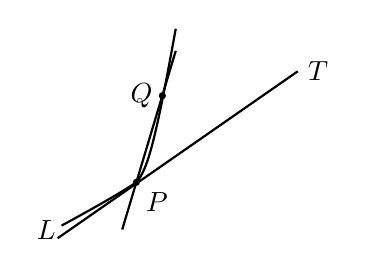
\begin{tikzpicture}[baseline=(current bounding box.center)]
  \coordinate (P) at (1.0,1.05);
  \coordinate (Q) at (1.33,2.15);
  % curve L through P
  \draw[thick] (0.05,0.5) .. controls (0.6,0.8) and (0.85,0.95) .. (P)
    .. controls (1.15,1.22) and (1.25,1.62) .. (1.5,3.0);
  % tangent at P
  \draw[thick] (0.0,0.34) -- (3.05,2.46) node[right] {$T$};
  % secant PQ
  \draw[thick] (0.82,0.45) -- (1.5,2.72);
  \fill (P) circle (1.3pt) node[below right] {$P$};
  \fill (Q) circle (1.3pt) node[left] {$Q$};
  \node[left] at (0.1,0.45) {$L$};
\end{tikzpicture}\caption{\relax}\label{fig:16-5}
\end{figure}

令 $t\to t_{0}$ 取极限，这时 $Q$ 趋于 $P$ 点，于是割线就变成为切线，从而割线上的向量就趋于切向量．故曲线在 $P$ 点的切向量为
\begin{equation}
\bm{\tau}=\pm\left(x^{\prime}(t_{0}),y^{\prime}(t_{0}),z^{\prime}(t_{0})\right).
\tag{1}
\end{equation}
特别地，若曲线 $L$ 由方程
\[
y=y(x),\ z=z(x),\ a\leqslant x\leqslant b
\]
给出，则这时可视 $x$ 为参数，即有参数方程
\[
L\colon\ x=x,\quad y=y(x),\quad z=z(x),\quad a\leqslant x\leqslant b.
\]
当 $x=x_{0}$ 时，记 $y_{0}=y(x_{0})$，$z_{0}=z(x_{0})$，这时由（1）式，曲线在 $P(x_{0},y_{0},z_{0})$ 点的切向量可取为
\begin{equation}
\bm{\tau}=\pm\left(1,y^{\prime}(x_{0}),z^{\prime}(x_{0})\right).
\tag{2}
\end{equation}
更一般地，若曲线用两曲面的交线给出
\[
L\colon\begin{cases}
F(x,y,z)=0,\\
G(x,y,z)=0,
\end{cases}
\]
$P(x_{0},y_{0},z_{0})$ 是曲线 $L$ 上的点．设上述方程组在 $P$ 点的某邻域内能确定函数组 $y=y(x)$，$z=z(x)$ 满足 $y_{0}=y(x_{0})$，$z_{0}=z(x_{0})$，且 $y^{\prime}(x)$ 和 $z^{\prime}(x)$ 存在，则由（2）式，只要求出 $y^{\prime}(x_{0})$ 和 $z^{\prime}(x_{0})$ 便可得到曲线在 $P$ 点的切向量．由隐函数组求导法，在方程两边对 $x$ 求导数，得
\[
\begin{cases}
F_{x}+F_{y}y^{\prime}+F_{z}z^{\prime}=0,\\
G_{x}+G_{y}y^{\prime}+G_{z}z^{\prime}=0.
\end{cases}
\]
当雅可比行列式 $\left.\dfrac{\partial(F,G)}{\partial(y,z)}\right|_{P}\neq 0$ 时，解得
\[
y^{\prime}(x_{0})=\left.\frac{\dfrac{\partial(F,G)}{\partial(z,x)}}{\dfrac{\partial(F,G)}{\partial(y,z)}}\right|_{P},\quad z^{\prime}(x_{0})=\left.\frac{\dfrac{\partial(F,G)}{\partial(x,y)}}{\dfrac{\partial(F,G)}{\partial(y,z)}}\right|_{P},
\]
代入（2）式得曲线在 $P(x_{0},y_{0},z_{0})$ 点的切向量
\[
\bm{\tau}=\pm\left(1,\ \frac{\dfrac{\partial(F,G)}{\partial(z,x)}}{\dfrac{\partial(F,G)}{\partial(y,z)}},\ \frac{\dfrac{\partial(F,G)}{\partial(x,y)}}{\dfrac{\partial(F,G)}{\partial(y,z)}}\right)\bigg|_{P}.
\]
也可取与之平行的向量
\begin{equation}
\bm{\tau}=\pm\left(\frac{\partial(F,G)}{\partial(y,z)},\frac{\partial(F,G)}{\partial(z,x)},\frac{\partial(F,G)}{\partial(x,y)}\right)\bigg|_{P}.
\tag{3}
\end{equation}

\begin{example}\label{ex:16-3-1}
求两柱面 $x^{2}+y^{2}=R^{2}$，$x^{2}+z^{2}=R^{2}$ 的交线在点 $\left(\dfrac{R}{\sqrt{2}},\dfrac{R}{\sqrt{2}},\dfrac{R}{\sqrt{2}}\right)$ 处的切线方程和法平面方程．
\end{example}

\begin{proof}[解]
令
\[
\begin{cases}
F(x,y,z)=x^{2}+y^{2}-R^{2},\\
G(x,y,z)=x^{2}+z^{2}-R^{2}.
\end{cases}
\]
这时曲线方程为
\[
\begin{cases}
F(x,y,z)=0,\\
G(x,y,z)=0.
\end{cases}
\]
由
\[
\begin{pmatrix}F_{x}&F_{y}&F_{z}\\ G_{x}&G_{y}&G_{z}\end{pmatrix}=\begin{pmatrix}2x&2y&0\\ 2x&0&2z\end{pmatrix}
\]
知
\[
\frac{\partial(F,G)}{\partial(y,z)}=\begin{vmatrix}2y&0\\ 0&2z\end{vmatrix}=4yz,
\]
\[
\frac{\partial(F,G)}{\partial(z,x)}=\begin{vmatrix}0&2x\\ 2z&2x\end{vmatrix}=-4xz,
\]
\[
\frac{\partial(F,G)}{\partial(x,y)}=\begin{vmatrix}2x&2y\\ 2x&0\end{vmatrix}=-4xy.
\]

\begin{figure}[htbp]
\centering
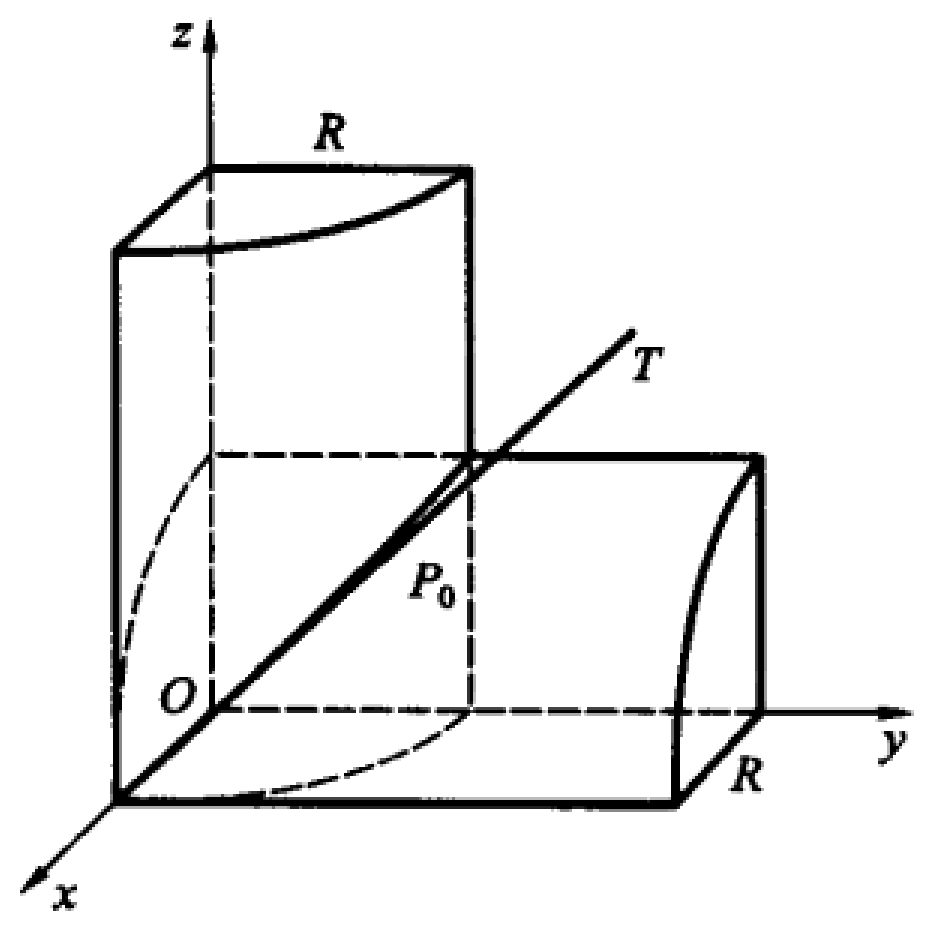
\includegraphics[width=0.5\textwidth]{work/figures/fig16-6}\caption{\relax}\label{fig:16-6}
\end{figure}

因此曲线在 $\left(\dfrac{R}{\sqrt{2}},\dfrac{R}{\sqrt{2}},\dfrac{R}{\sqrt{2}}\right)$ 处的切向量为
\[
\begin{aligned}
\bm{\tau}&=\left.(yz,-xz,-xy)\right|_{\left(\frac{R}{\sqrt{2}},\frac{R}{\sqrt{2}},\frac{R}{\sqrt{2}}\right)}\\
&=\frac{R^{2}}{2}(1,-1,-1),
\end{aligned}
\]
故曲线在 $\left(\dfrac{R}{\sqrt{2}},\dfrac{R}{\sqrt{2}},\dfrac{R}{\sqrt{2}}\right)$ 的切线方程为
\[
x-\frac{R}{\sqrt{2}}=\frac{y-\dfrac{R}{\sqrt{2}}}{-1}=\frac{z-\dfrac{R}{\sqrt{2}}}{-1},
\]
即
\[
\frac{R}{\sqrt{2}}-x=y-\frac{R}{\sqrt{2}}=z-\frac{R}{\sqrt{2}},
\]
而法平面方程为
\[
\left(x-\frac{R}{\sqrt{2}}\right)-\left(y-\frac{R}{\sqrt{2}}\right)-\left(z-\frac{R}{\sqrt{2}}\right)=0,
\]
即
\[
x-y-z+\frac{R}{\sqrt{2}}=0.
\]
\end{proof}

\subsection{空间曲面的切平面与法线}

求空间曲面的切平面与法线，关键在于求切平面的法向量 $\bm{n}$．若已知曲面上一点 $P(x_{0},y_{0},z_{0})$ 处切平面的法向量为
\[
\bm{n}=(A^{\prime},B^{\prime},C^{\prime}),
\]
则曲面在该点的切平面方程为
\[
A^{\prime}(x-x_{0})+B^{\prime}(y-y_{0})+C^{\prime}(z-z_{0})=0.
\]
曲面在该点的法线方程为
\[
\frac{x-x_{0}}{A^{\prime}}=\frac{y-y_{0}}{B^{\prime}}=\frac{z-z_{0}}{C^{\prime}}.
\]
因此下面我们只讨论如何求曲面的法向量 $\bm{n}$．

设曲面方程为
\[
\pi\colon F(x,y,z)=0.
\]
在曲面上任取一条过 $P$ 点的曲线，设其方程为
\[
x=x(t),\ y=y(t),\ z=z(t),
\]
这时有
\[
F(x(t),y(t),z(t))=0.
\]
设 $t=t_{0}$ 对应于点 $P(x_{0},y_{0},z_{0})$，由复合函数求导法，两边对 $t$ 求导并令 $t=t_{0}$，得
\[
F_{x}(x_{0},y_{0},z_{0})x^{\prime}(t_{0})+F_{y}(x_{0},y_{0},z_{0})y^{\prime}(t_{0})+F_{z}(x_{0},y_{0},z_{0})z^{\prime}(t_{0})=0.
\]
写成向量的内积形式
\[
(F_{x},F_{y},F_{z})_{P}\cdot(x^{\prime}(t_{0}),y^{\prime}(t_{0}),z^{\prime}(t_{0}))=0.
\]
上式表明向量 $(F_{x},F_{y},F_{z})_{P}$ 与曲面上任一过 $P$ 点的曲线在 $P$ 点的切线垂直，因此这些切线在同一平面上，这平面就是曲面在 $P$ 点的切平面，而这个切平面的法向量就是
\begin{equation}
\bm{n}=\pm(F_{x},F_{y},F_{z})_{P},
\tag{4}
\end{equation}
它也称为曲面在 $P$ 的法向量．

特别地，若曲面方程为
\[
\pi\colon z=f(x,y),
\]
则只要令
\[
F(x,y,z)=f(x,y)-z,
\]
由（4）式即得曲面在 $P$ 点的法向量为
\begin{equation}
\bm{n}=\pm\left(f_{x},f_{y},-1\right)_{(x_{0},y_{0},z_{0})}.
\tag{5}
\end{equation}

最后，设曲面由参数方程给出
\[
\pi\colon\begin{cases}
x=x(u,v),\\
y=y(u,v),\\
z=z(u,v).
\end{cases}
\]
当 $(u,v)=(u_{0},v_{0})$ 时对应曲面上的点 $P(x_{0},y_{0},z_{0})$．若方程组 $x=x(u,v)$，$y=y(u,v)$ 可确定函数组 $u=u(x,y)$，$v=v(x,y)$，满足 $u_{0}=u(x_{0},y_{0})$，$v_{0}=v(x_{0},y_{0})$，代入 $z=z(u,v)$，则 $z$ 是 $x$、$y$ 的函数 $z=z(u(x,y),v(x,y))$ 且 $z_{0}=z(u(x_{0},y_{0}),v(x_{0},y_{0}))$．于是由（5）式，只要求出 $\left.\dfrac{\partial z}{\partial x}\right|_{P}$ 和 $\left.\dfrac{\partial z}{\partial y}\right|_{P}$ 便可得曲面在 $P$ 点的法向量．为此，我们用隐函数求导法求 $z=z(u,v)$ 对 $u$，$v$ 的偏导数，得
\[
\begin{cases}
\dfrac{\partial z}{\partial u}=\dfrac{\partial z}{\partial x}\dfrac{\partial x}{\partial u}+\dfrac{\partial z}{\partial y}\dfrac{\partial y}{\partial u},\\[8pt]
\dfrac{\partial z}{\partial v}=\dfrac{\partial z}{\partial x}\dfrac{\partial x}{\partial v}+\dfrac{\partial z}{\partial y}\dfrac{\partial y}{\partial v},
\end{cases}
\]
这是关于 $\dfrac{\partial z}{\partial x}$，$\dfrac{\partial z}{\partial y}$ 的线性方程组，当雅可比行列式 $\left.\dfrac{\partial(x,y)}{\partial(u,v)}\right|_{P}\neq 0$ 时，由克拉默法则解得
\[
\left.\frac{\partial z}{\partial x}\right|_{P}=-\left.\frac{\dfrac{\partial(y,z)}{\partial(u,v)}}{\dfrac{\partial(x,y)}{\partial(u,v)}}\right|_{P},\quad \left.\frac{\partial z}{\partial y}\right|_{P}=-\left.\frac{\dfrac{\partial(z,x)}{\partial(u,v)}}{\dfrac{\partial(x,y)}{\partial(u,v)}}\right|_{P}.
\]
代入（5）式并消去公共因子，即得曲面在 $P$ 点的法向量
\begin{equation}
\bm{n}=\pm\left(\frac{\partial(y,z)}{\partial(u,v)},\frac{\partial(z,x)}{\partial(u,v)},\frac{\partial(x,y)}{\partial(u,v)}\right)\bigg|_{P}.
\tag{6}
\end{equation}

\begin{example}\label{ex:16-3-2}
求椭球面 $x^{2}+2y^{2}+3z^{2}=6$ 在 $(1,1,1)$ 点的切平面方程与法线方程．
\end{example}

\begin{proof}[解]
令 $F(x,y,z)=x^{2}+2y^{2}+3z^{2}-6$，则
\[
\begin{aligned}
\bm{n}&=\left.(F_{x},F_{y},F_{z})\right|_{(1,1,1)}\\
&=\left.(2x,4y,6z)\right|_{(1,1,1)}\\
&=2(1,2,3),
\end{aligned}
\]
故所求的切平面方程为
\[
(x-1)+2(y-1)+3(z-1)=0,
\]
即
\[
x+2y+3z-6=0,
\]
而法线方程为
\[
\frac{x-1}{1}=\frac{y-1}{2}=\frac{z-1}{3}.
\]
\end{proof}

\begin{example}\label{ex:16-3-3}
求球面
\[
\begin{cases}
x=\cos\theta\sin\varphi,\\
y=\sin\theta\sin\varphi,\\
z=\cos\varphi
\end{cases}
\]
在对应于 $\theta=\varphi=\dfrac{\pi}{4}$ 处的切平面方程和法线方程．
\end{example}

\begin{proof}[解]
用公式（6）．由
\[
\begin{pmatrix}\dfrac{\partial x}{\partial\theta}&\dfrac{\partial y}{\partial\theta}&\dfrac{\partial z}{\partial\theta}\\[6pt]
\dfrac{\partial x}{\partial\varphi}&\dfrac{\partial y}{\partial\varphi}&\dfrac{\partial z}{\partial\varphi}\end{pmatrix}=\begin{pmatrix}-\sin\theta\sin\varphi&\cos\theta\sin\varphi&0\\ \cos\theta\cos\varphi&\sin\theta\cos\varphi&-\sin\varphi\end{pmatrix},
\]
知
\[
\left.\frac{\partial(y,z)}{\partial(\theta,\varphi)}\right|_{\left(\frac{\pi}{4},\frac{\pi}{4}\right)}=\left.-\cos\theta\sin^{2}\varphi\right|_{\left(\frac{\pi}{4},\frac{\pi}{4}\right)}=-\frac{\sqrt{2}}{4},
\]
\[
\left.\frac{\partial(z,x)}{\partial(\theta,\varphi)}\right|_{\left(\frac{\pi}{4},\frac{\pi}{4}\right)}=\left.-\sin\theta\sin^{2}\varphi\right|_{\left(\frac{\pi}{4},\frac{\pi}{4}\right)}=-\frac{\sqrt{2}}{4},
\]
\[
\left.\frac{\partial(x,y)}{\partial(\theta,\varphi)}\right|_{\left(\frac{\pi}{4},\frac{\pi}{4}\right)}=\left.-\sin\varphi\cos\varphi\right|_{\left(\frac{\pi}{4},\frac{\pi}{4}\right)}=-\frac{1}{2},
\]
从而
\[
\bm{n}=-\frac{\sqrt{2}}{4}(1,1,\sqrt{2}).
\]
又 $\theta=\varphi=\dfrac{\pi}{4}$ 时 $(x,y,z)=\left(\dfrac{1}{2},\dfrac{1}{2},\dfrac{\sqrt{2}}{2}\right)$，故所求的切平面方程为
\[
\left(x-\frac{1}{2}\right)+\left(y-\frac{1}{2}\right)+\sqrt{2}\left(z-\frac{\sqrt{2}}{2}\right)=0,
\]
即
\[
x+y+\sqrt{2}z-2=0,
\]
而法线方程为
\[
x-\frac{1}{2}=y-\frac{1}{2}=\frac{1}{\sqrt{2}}\left(z-\frac{\sqrt{2}}{2}\right).
\]
\end{proof}

\begin{xiti}
\item 求下列曲线在所示点处的切线方程和法平面方程：
\begin{ziti}
\item $x=a\sin^{2}t$，$y=b\sin t\cos t$，$z=c\cos^{2}t$，在点 $t=\dfrac{\pi}{4}$；
\item $2x^{2}+3y^{2}+z^{2}=9$，$z^{2}=3x^{2}+y^{2}$，在点 $(1,-1,2)$；
\item $x^{2}+y^{2}+z^{2}=6$，$x+y+z=0$，在点 $(1,-2,1)$；
\item $x=t-\cos t$，$y=3+\sin^{2}t$，$z=1+\cos 3t$，在点 $t=\dfrac{\pi}{2}$．
\end{ziti}
\item 求下列曲面在所示点处的切平面方程和法线方程：
\begin{ziti}
\item $y-\mathrm{e}^{2x-z}=0$，在点 $(1,1,2)$；
\item $\dfrac{x^{2}}{a^{2}}+\dfrac{y^{2}}{b^{2}}+\dfrac{z^{2}}{c^{2}}=1$ 在点 $\left(\dfrac{a}{\sqrt{3}},\dfrac{b}{\sqrt{3}},\dfrac{c}{\sqrt{3}}\right)$；
\item $z=2x^{2}+4y^{2}$ 在点 $(2,1,12)$；
\item $x=u\cos v$，$y=u\sin v$，$z=av$ 在点 $P_{0}(u_{0},v_{0})$．
\end{ziti}
\item 证明曲线 $x=a\mathrm{e}^{t}\cos t$，$y=a\mathrm{e}^{t}\sin t$，$z=a\mathrm{e}^{t}$ 与锥面 $x^{2}+y^{2}=z^{2}$ 的母线相交成同一角度．
\item 求平面曲线 $x^{2/3}+y^{2/3}=a^{2/3}$ $(a>0)$ 上任一点处的切线方程，并证明这些切线被坐标轴所截取的线段等长．
\item 求曲面 $x^{2}+2y^{2}+3z^{2}=21$ 的切平面，使它平行于平面 $x+4y+6z=0$．
\item 证明：曲面 $F(x-az,y-bz)=0$ 的切平面与某一定直线平行，其中 $a$，$b$ 为常数．
\item 证明曲面 $z=x\mathrm{e}^{\frac{x}{y}}$ 的每一切平面都通过原点．
\item 求两曲面
\[
F(x,y,z)=0,\quad G(x,y,z)=0
\]
的交线在 $Oxy$ 平面上的投影曲线的切线方程．
\end{xiti}

\section{方向导数}

我们已经知道，偏导数给出的是函数沿坐标轴方向的变化率．然而许多实际问题中常常希望知道函数沿任意方向的变化率．例如热量的传导、空气的流动、气压的改变等，沿各个方向的变化率一般是不一样的．下面我们仿照偏导数的定义，引出方向导数的概念．

设函数 $u=f(x,y,z)$，其定义域是空间某区域．在定义域中任取点 $P_{0}(x_{0},y_{0},z_{0})$，由偏导数的定义知，函数 $u$ 在 $P_{0}$ 点关于 $x$ 的偏导数定义为
\[
\left.\frac{\partial u}{\partial x}\right|_{P_{0}}=\lim_{\Delta x\to 0}\frac{f(x_{0}+\Delta x,y_{0},z_{0})-f(x_{0},y_{0},z_{0})}{\Delta x}.
\]
考虑 $\Delta x>0$，并记 $P=(x_{0}+\Delta x,y_{0},z_{0})$，这时 $\Delta x$ 就是 $P$ 与 $P_{0}$ 点的距离 $r(P,P_{0})$．于是上面的极限可用点 $P$ 和 $P_{0}$ 表示为
\[
\lim_{r(P,P_{0})\to 0}\frac{f(P)-f(P_{0})}{r(P,P_{0})}.
\]
注意这里 $P$ 点是始于 $P_{0}$ 点且与 $x$ 轴同方向的射线上的点．如果将 $P$ 点限制在始于 $P_{0}$ 点的另一射线上的点，便得到方向导数的定义．

\begin{figure}[htbp]
\centering
\begin{tikzpicture}[baseline=(current bounding box.center)]
  \coordinate (O) at (0.95,0.05);
  \coordinate (P0) at (1.7,2.3);
  \coordinate (Px) at (0.95,1.8);
  \coordinate (Py) at (3.2,2.3);
  \coordinate (P) at (2.55,1.8);
  \coordinate (B) at (1.7,1.4);
  \coordinate (Bx) at (0.95,0.9);
  \coordinate (By) at (3.2,1.4);
  \coordinate (Bxy) at (2.55,0.9);
  \draw[thick,{-Latex}] (O) -- (0.95,3.2) node[above] {$z$};
  \draw[thick,{-Latex}] (O) -- (3.7,0.05) node[right] {$y$};
  \draw[thick,{-Latex}] (O) -- (0.2,-0.55) node[below] {$x$};
  \node[above left] at (0.9,0.02) {$O$};
  \draw[dashed] (P0) -- (Py) -- (P) -- (Px) -- cycle;
  \draw[dashed] (B) -- (By) -- (Bxy) -- (Bx) -- cycle;
  \draw[dashed] (P0) -- (B) (Py) -- (By) (P) -- (Bxy) (Px) -- (Bx);
  \draw[thick,{-Latex}] (P0) -- (3.45,1.27) node[right] {$\bm{l}$};
  \fill (P0) circle (1.3pt) node[above left] {$P_{0}$};
  \fill (P) circle (1.3pt) node[above right] {$P$};
  \node[left] at (1.66,1.85) {$\Delta z$};
  \node[below left] at (1.32,1.12) {$\Delta x$};
  \node[below] at (1.75,0.9) {$\Delta y$};
\end{tikzpicture}\caption{\relax}\label{fig:16-7}
\end{figure}

\begin{definition}\label{def:16-3}
设三元函数 $u=f(x,y,z)$ 在点 $P_{0}(x_{0},y_{0},z_{0})$ 的某邻域内有定义，任意给定始于点 $P_{0}$ 的射线 $\bm{l}$，$P(x,y,z)$ 为 $\bm{l}$ 上且含于定义域内的点．若极限
\[
\lim_{r(P,P_{0})\to 0^{+}}\frac{f(P)-f(P_{0})}{r(P,P_{0})}=\lim_{r(P,P_{0})\to 0^{+}}\frac{\Delta_{l}f(P_{0})}{r(P,P_{0})}
\]
存在，则称该极限值为函数 $f$ 在点 $P_{0}$ 沿方向 $\bm{l}$ 的方向导数，记为 $\left.\dfrac{\partial f}{\partial l}\right|_{P_{0}}$ 或
\[
\frac{\partial f(P_{0})}{\partial l}.
\]
\end{definition}

$\Delta_{l}f(P_{0})$ 称为函数在 $P_{0}$ 点沿 $\bm{l}$ 方向的增量．若 $\bm{l}$ 的方向余弦为
\[
\bm{l}_{0}=(\cos\alpha,\cos\beta,\cos\gamma),
\]
$P$ 点为 $(x_{0}+\Delta x,y_{0}+\Delta y,z_{0}+\Delta z)$，这时 $\Delta x$，$\Delta y$，$\Delta z$ 不是独立的，它们满足
\[
\frac{\Delta x}{\cos\alpha}=\frac{\Delta y}{\cos\beta}=\frac{\Delta z}{\cos\gamma},
\]
或
\[
\begin{aligned}
\bm{l}_{0}&=(\cos\alpha,\cos\beta,\cos\gamma)\\
&=\frac{1}{\rho}(\Delta x,\Delta y,\Delta z),
\end{aligned}
\]
其中
\[
\rho=r(P,P_{0})=\sqrt{(\Delta x)^{2}+(\Delta y)^{2}+(\Delta z)^{2}}.
\]
当 $\Delta y=\Delta z=0$ 时，$\bm{l}$ 的方向即为 $x$ 轴的正向 $(\Delta x>0)$ 或负向 $(\Delta x<0)$．若 $\Delta x>0$，则
\[
\frac{\partial f(P_{0})}{\partial l}=\frac{\partial f(P_{0})}{\partial x}.
\]
即 $\dfrac{\partial f(P_{0})}{\partial x}$ 就是函数在 $P_{0}$ 点沿 $x$ 轴正向的方向导数．同理 $\dfrac{\partial f(P_{0})}{\partial y}$，$\dfrac{\partial f(P_{0})}{\partial z}$ 分别是函数在 $P_{0}$ 点的沿 $y$ 轴和 $z$ 轴正方向的方向导数．

下面的定理提供了方向导数的简便计算方法．

\begin{theorem}\label{thm:16-6}
若函数 $f(x,y,z)$ 在点 $P_{0}(x_{0},y_{0},z_{0})$ 可微，则 $f(x,y,z)$ 在点 $P_{0}$ 沿任何方向 $\bm{l}$ 的方向导数都存在，且有以下公式
\[
\frac{\partial f(P_{0})}{\partial l}=\frac{\partial f(P_{0})}{\partial x}\cos\alpha+\frac{\partial f(P_{0})}{\partial y}\cos\beta+\frac{\partial f(P_{0})}{\partial z}\cos\gamma.
\]
其中 $\cos\alpha,\cos\beta,\cos\gamma$ 是 $\bm{l}$ 的方向余弦．
\end{theorem}

\begin{proof}
设 $P(x,y,z)$ 是射线 $\bm{l}$ 上的任一点，则
\[
\begin{cases}
x-x_{0}=\Delta x=\rho\cos\alpha,\\
y-y_{0}=\Delta y=\rho\cos\beta,\\
z-z_{0}=\Delta z=\rho\cos\gamma.
\end{cases}
\]
$\rho=\sqrt{(\Delta x)^{2}+(\Delta y)^{2}+(\Delta z)^{2}}$．由于函数 $f(x,y,z)$ 在 $P_{0}(x_{0},y_{0},z_{0})$ 可微，由定义有
\[
f(P)-f(P_{0})=\frac{\partial f(P_{0})}{\partial x}\Delta x+\frac{\partial f(P_{0})}{\partial y}\Delta y+\frac{\partial f(P_{0})}{\partial z}\Delta z+o(\rho)
\]
对任意 $\Delta x$，$\Delta y$，$\Delta z$ 都成立，特别对满足上述关系的 $\Delta x$，$\Delta y$，$\Delta z$ 有
\[
\begin{aligned}
\frac{f(P)-f(P_{0})}{\rho}&=\frac{\partial f(P_{0})}{\partial x}\frac{\Delta x}{\rho}+\frac{\partial f(P_{0})}{\partial y}\frac{\Delta y}{\rho}+\frac{\partial f(P_{0})}{\partial z}\frac{\Delta z}{\rho}+\frac{o(\rho)}{\rho}\\
&=\frac{\partial f(P_{0})}{\partial x}\cos\alpha+\frac{\partial f(P_{0})}{\partial y}\cos\beta+\frac{\partial f(P_{0})}{\partial z}\cos\gamma+\frac{o(\rho)}{\rho}.
\end{aligned}
\]
令 $\rho\to 0$ 取极限即得
\[
\frac{\partial f(P_{0})}{\partial l}=\frac{\partial f(P_{0})}{\partial x}\cos\alpha+\frac{\partial f(P_{0})}{\partial y}\cos\beta+\frac{\partial f(P_{0})}{\partial z}\cos\gamma.
\]
定理~\ref{thm:16-6} 证完．
\end{proof}

定理中的公式又可用矢量的内积表示为
\[
\frac{\partial f(P_{0})}{\partial l}=\left(\frac{\partial f}{\partial x},\frac{\partial f}{\partial y},\frac{\partial f}{\partial z}\right)\bigg|_{P_{0}}\cdot(\cos\alpha,\cos\beta,\cos\gamma).
\]

对于二元函数 $u=f(x,y)$，它在 $P_{0}(x_{0},y_{0})$ 点沿任一方向 $\bm{l}=(\cos\alpha,\cos\beta)$ 的方向导数为
\[
\begin{aligned}
\frac{\partial f(x_{0},y_{0})}{\partial l}&=\frac{\partial f(x_{0},y_{0})}{\partial x}\cos\alpha+\frac{\partial f(x_{0},y_{0})}{\partial y}\cos\beta\\
&=\left(\frac{\partial f}{\partial x},\frac{\partial f}{\partial y}\right)\bigg|_{(x_{0},y_{0})}\cdot(\cos\alpha,\cos\beta).
\end{aligned}
\]

\begin{example}\label{ex:16-4-1}
求函数 $u=xy^{2}+z^{3}-xyz$ 在点 $(1,1,2)$ 处沿方向 $\bm{l}$ 的方向导数，$\bm{l}$ 的方向角分别为 $60^{\circ}$，$45^{\circ}$，$60^{\circ}$．
\end{example}

\begin{proof}[解]
$\bm{l}$ 的方向余弦为
\[
(\cos 60^{\circ},\cos 45^{\circ},\cos 60^{\circ})=\left(\frac{1}{2},\frac{\sqrt{2}}{2},\frac{1}{2}\right).
\]
又
\[
\begin{aligned}
&\left(\frac{\partial u}{\partial x},\frac{\partial u}{\partial y},\frac{\partial u}{\partial z}\right)\bigg|_{(1,1,2)}\\
&=\left(y^{2}-yz,2xy-xz,3z^{2}-xy\right)|_{(1,1,2)}\\
&=(-1,0,11).
\end{aligned}
\]
故
\[
\left.\frac{\partial u}{\partial l}\right|_{(1,1,2)}=(-1,0,11)\cdot\left(\frac{1}{2},\frac{\sqrt{2}}{2},\frac{1}{2}\right)=5.
\]
\end{proof}

\begin{xiti}
\item 设 $f(x,y,z)=x+y^{2}+z^{3}$，求 $f$ 在点 $P_{0}(1,1,1)$ 沿方向 $\bm{l}=(2,-2,1)$ 的方向导数．
\item 求函数 $u=xyz$ 在点 $A(5,1,2)$ 处沿到点 $B(9,4,14)$ 的方向 $\overrightarrow{AB}$ 上的方向导数．
\item 求 $\left.\dfrac{\partial u}{\partial l}\right|_{(x_{0},y_{0})}$：
\begin{ziti}
\item $u=\ln\left(x^{2}+y^{2}\right)$，$(x_{0},y_{0})=(1,1)$，$\bm{l}$ 与 $x$ 轴正向的夹角为 $60^{\circ}$；
\item $u=x\mathrm{e}^{xy}$，$(x_{0},y_{0})=(1,1)$，$\bm{l}$ 与向量 $(1,1)$ 同向．
\end{ziti}
\item 设函数 $f(x,y)$ 在 $(x_{0},y_{0})$ 可微，单位向量 $\bm{l}_{1}=\left(\dfrac{1}{\sqrt{2}},\dfrac{1}{\sqrt{2}}\right)$，$\bm{l}_{2}=\left(-\dfrac{1}{\sqrt{2}},\dfrac{1}{\sqrt{2}}\right)$，$\dfrac{\partial f(x_{0},y_{0})}{\partial l_{1}}=1$，$\dfrac{\partial f(x_{0},y_{0})}{\partial l_{2}}=0$，确定 $\bm{l}$ 使得
\[
\frac{\partial f(x_{0},y_{0})}{\partial l}=\frac{7}{5\sqrt{2}}.
\]
\item 设 $f$ 在 $P_{0}(2,0)$ 可微，$f(x,y)$ 在 $P_{0}$ 指向 $P_{1}=(2,-2)$ 的方向导数是 $1$，指向原点的方向导数是 $-3$，试回答：
\begin{ziti}
\item 指向 $P_{2}=(2,1)$ 的方向导数是多少？
\item 指向 $P_{3}=(3,2)$ 的方向导数是多少？
\end{ziti}
\end{xiti}

\section{泰勒公式}

回忆一元函数的泰勒公式：若 $f(x)$ 在 $x_{0}$ 点的某邻域有 $n+1$ 阶连续微商，则当 $x=x_{0}+\Delta x$ 属于该邻域时，有
\begin{equation}
f\left(x_{0}+\Delta x\right)=\sum_{k=0}^{n}\frac{f^{(k)}\left(x_{0}\right)}{k!}\Delta x^{k}+R_{n}(x).
\tag{1}
\end{equation}
其中 $R_{n}(x)$ 可用拉格朗日余项形式表出
\[
R_{n}(x)=\frac{1}{(n+1)!}f^{(n+1)}\left(x_{0}+\theta\Delta x\right)\Delta x^{n+1},\quad 0<\theta<1.
\]

对于二元函数，有类似的结果成立．

\begin{theorem}[（泰勒定理）]\label{thm:16-7}
设 $f(x,y)$ 在 $P_{0}(x_{0},y_{0})$ 的某邻域 $O(P_{0})$ 内有直到 $n+1$ 阶连续偏导数，则对 $O(P_{0})$ 内任一点 $(x_{0}+\Delta x,y_{0}+\Delta y)$，存在 $\theta\in(0,1)$，使得
\begin{equation}
f\left(x_{0}+\Delta x,y_{0}+\Delta y\right)=\sum_{k=0}^{n}\frac{1}{k!}\left(\frac{\partial}{\partial x}\Delta x+\frac{\partial}{\partial y}\Delta y\right)^{k}f\left(x_{0},y_{0}\right)+R_{n},
\tag{2}
\end{equation}
其中
\[
R_{n}=\frac{1}{(n+1)!}\left(\frac{\partial}{\partial x}\Delta x+\frac{\partial}{\partial y}\Delta y\right)^{n+1}f\left(x_{0}+\theta\Delta x,y_{0}+\theta\Delta y\right).
\]
\end{theorem}

\begin{proof}
用一元函数的结果．引入参数 $t$，构造函数
\[
\varphi(t)=f\left(x_{0}+t\Delta x,y_{0}+t\Delta y\right),\quad t\in[0,1].
\]
这时 $\varphi(0)=f(x_{0},y_{0})$，$\varphi(1)=f(x_{0}+\Delta x,y_{0}+\Delta y)$．由 $f(x,y)$ 在 $O(P_{0})$ 内有直到 $n+1$ 阶连续偏导数，知复合函数 $\varphi(t)$ 在 $[0,1]$ 有直到 $n+1$ 阶的连续导数，且可用复合函数求导的链式法则求出
\[
\begin{aligned}
\varphi^{(k)}(t)&=\left(\frac{\partial}{\partial x}\Delta x+\frac{\partial}{\partial y}\Delta y\right)^{k}f\left(x_{0}+t\Delta x,y_{0}+t\Delta y\right),\\
&&k=1,2,\cdots,n+1.
\end{aligned}
\]
由一元函数拉格朗日型余项的泰勒公式，存在 $\theta\in(0,1)$，使得
\[
\varphi(1)=\sum_{k=0}^{n}\frac{\varphi^{(k)}(0)}{k!}+\frac{1}{(n+1)!}\varphi^{(n+1)}(\theta),
\]
即
\[
\begin{aligned}
&f\left(x_{0}+\Delta x,y_{0}+\Delta y\right)\\
={}&\sum_{k=0}^{n}\frac{1}{k!}\left(\frac{\partial}{\partial x}\Delta x+\frac{\partial}{\partial y}\Delta y\right)^{k}f\left(x_{0},y_{0}\right)+{}\\
&\frac{1}{(n+1)!}\left(\frac{\partial}{\partial x}\Delta x+\frac{\partial}{\partial y}\Delta y\right)^{n+1}f\left(x_{0}+\theta\Delta x,y_{0}+\theta\Delta y\right).
\end{aligned}
\]
定理~\ref{thm:16-7} 证完．
\end{proof}

公式 (2) 称为二元函数 $f(x,y)$ 在 $(x_{0},y_{0})$ 点的 $n$ 阶泰勒公式．式中的余项 $R_{n}$ 称为拉格朗日型余项．当 $n=0$ 时，就得到二元函数的中值公式：
\begin{equation}
\begin{aligned}
&f\left(x_{0}+\Delta x,y_{0}+\Delta y\right)-f\left(x_{0},y_{0}\right)\\
=\;&f_{x}\left(x_{0}+\theta\Delta x,y_{0}+\theta\Delta y\right)\Delta x+f_{y}\left(x_{0}+\theta\Delta x,y_{0}+\theta\Delta y\right)\Delta y,\\
&&0<\theta<1.
\end{aligned}
\tag{3}
\end{equation}

下面我们忽略余项，把 $n=0,1,2$ 的泰勒展开式写出来．
\[
\begin{aligned}
n=0,\qquad&f\left(x_{0}+\Delta x,y_{0}+\Delta y\right)\approx f\left(x_{0},y_{0}\right)\\
n=1,\qquad&f\left(x_{0}+\Delta x,y_{0}+\Delta y\right)\\
\approx\;&f\left(x_{0},y_{0}\right)+f_{x}\left(x_{0},y_{0}\right)\Delta x+f_{y}\left(x_{0},y_{0}\right)\Delta y,\\
n=2,\qquad&f\left(x_{0}+\Delta x,y_{0}+\Delta y\right)\\
\approx\;&f\left(x_{0},y_{0}\right)+f_{x}\left(x_{0},y_{0}\right)\Delta x+f_{y}\left(x_{0},y_{0}\right)\Delta y+\\
&\frac{1}{2}\left\{f_{xx}\left(x_{0},y_{0}\right)\Delta x^{2}+2f_{xy}\left(x_{0},y_{0}\right)\Delta x\Delta y+f_{yy}\left(x_{0},y_{0}\right)\Delta y^{2}\right\}.
\end{aligned}
\]
$n=1$ 时，正是用函数的微分代替函数的改变量．

\begin{example}\label{ex:16-5-1}
设 $f(x,y)=x^{y}$，利用 $f(x,y)$ 在点 $(1,4)$ 的二阶泰勒公式，近似计算 $(1.08)^{3.96}$．
\end{example}

\begin{proof}[解]
\[
\begin{aligned}
&f(x,y)=x^{y},\qquad\qquad\qquad\qquad\ \ f(1,4)=1\,;\\
&f_{x}(x,y)=yx^{y-1},\qquad\qquad\qquad\ \ f_{x}(1,4)=4\,;\\
&f_{y}(x,y)=x^{y}\ln x,\qquad\qquad\qquad\ \ f_{y}(1,4)=0\,;\\
&f_{x^{2}}(x,y)=y(y-1)x^{y-2},\qquad\quad f_{x^{2}}(1,4)=12\,;\\
&f_{xy}(x,y)=x^{y-1}+yx^{y-1}\ln x,\qquad\ \ f_{xy}(1,4)=1\,;\\
&f_{y^{2}}(x,y)=x^{y}\ln^{2}x,\qquad\qquad\quad\;\; f_{y^{2}}(1,4)=0.
\end{aligned}
\]
\[
\begin{aligned}
x^{y}\approx\;&f(1,4)+f_{x}(1,4)(x-1)+f_{y}(1,4)(y-4)+\\
&\frac{1}{2!}\left[f_{x^{2}}(1,4)(x-1)^{2}+2f_{xy}(1,4)(x-1)(y-4)+\right.\\
&\left.f_{y^{2}}(1,4)(y-4)^{2}\right]\\
=\;&1+4(x-1)+6(x-1)^{2}+(x-1)(y-4),
\end{aligned}
\]
取 $x=1.08$，$y=3.96$，得
\[
\begin{aligned}
1.08^{3.96}&\approx 1+4\times 0.08+6\times 0.08^{2}+0.08(-0.04)\\
&=1.355\ 2.
\end{aligned}
\]
\end{proof}

在本章 §1 中，我们曾用全微分近似函数的改变量，或说用一阶多项式逼近函数 $f(x,y)$，计算过 $1.08^{3.96}$ 的近似值为 $1.08^{3.96}\approx 1.32$．现在我们是用二阶多项式逼近函数 $f(x,y)$，得近似值 $1.08^{3.96}\approx 1.355\ 2$，比前面稍为精确了一些．利用泰勒公式，我们还可用 $n$ 阶多项式逼近函数 $f(x,y)$，$n$ 越大则误差越小，近似程度越好．

\begin{xiti}
\item 写出下列函数在指定点的泰勒公式：
\begin{ziti}
\item $f(x,y)=2x^{2}-xy-y^{2}-6x-3y+5$，在 $(1,-2)$ 点；
\item $f(x,y)=x^{2}+xy+y^{2}+3x-2y+4$，在 $(-1,1)$ 点．
\end{ziti}
\item 求函数 $f(x,y)=\dfrac{x}{y}$ 在 $(1,1)$ 点邻域的 $n$ 阶带拉格朗日余项的泰勒公式．
\item 求函数 $f(x,y)=\dfrac{y^{2}}{x^{2}}$ 在 $(1,-1)$ 点邻域的二阶泰勒公式，并写出拉格朗日余项．
\item 求下列函数在 $(0,0)$ 点邻域的四阶泰勒公式：
\begin{ziti}
\item $f(x,y)=\sin\left(x^{2}+y^{2}\right)$；
\item $f(x,y)=\mathrm{e}^{x}\ln(1+y)$；
\item $f(x,y)=\sqrt{1+x^{2}+y^{2}}$；
\item $f(x,y)=\mathrm{e}^{x}\cos y$．
\end{ziti}
\item 证明泰勒公式的唯一性：若
\[
\sum_{i+j=0}^{n}A_{ij}x^{i}y^{j}+o\left(\rho^{n}\right)=0\quad(\rho\to 0),
\]
其中 $\rho=\sqrt{x^{2}+y^{2}}$．求证 $A_{ij}=0$（$i,j$ 为非负整数，$i+j=0,1,\cdots,n$），并利用唯一性求 $f(x,y)=\ln(1+x+y)$ 在 $(0,0)$ 点带拉格朗日余项的 $n$ 阶泰勒展开式．
\item 通过对 $f(x,y)=\sin x\cos y$ 用中值定理，证明存在 $\theta\in(0,1)$，使
\[
\frac{3}{4}=\frac{\pi}{3}\cos\frac{\pi\theta}{3}\cos\frac{\pi\theta}{6}-\frac{\pi}{6}\sin\frac{\pi\theta}{3}\sin\frac{\pi\theta}{6}.
\]
\item 设 $f(x,y)$ 在区域 $D$ 内有偏导数存在，且 $f_{x}(x,y)=f_{y}(x,y)\equiv 0$．证明 $f(x,y)$ 在 $D$ 内为常数．
\item 若 $\left|x\right|$，$\left|y\right|$ 是很小的量，导出下列函数准确到二次项的近似公式：
\begin{ziti}
\item $\dfrac{\cos x}{\cos y}$；
\item $\arctan\dfrac{1+x+y}{1-xy}$．
\end{ziti}
\item 设函数 $f(x,y)$ 有直到 $n$ 阶连续偏导数，试证 $u(t)=f(a+ht,b+kt)$ 的 $n$ 阶导数
\[
u^{(n)}(t)=\left(h\frac{\partial}{\partial x}+k\frac{\partial}{\partial y}\right)^{n}f(a+ht,b+kt).
\]
\item 设 $f(x,y)$ 为 $n$ 次齐次函数，证明
\[
\left(x\frac{\partial}{\partial x}+y\frac{\partial}{\partial y}\right)^{m}f=n(n-1)\cdots(n-m+1)f.
\]
\item 设 $f(x,y)=\psi(ax+by)$，其中 $a$，$b$ 为常数，在包含原点的某邻域内，$\psi$ 有 $q$ 阶连续导数．求证：在 $(0,0)$ 点邻域的泰勒公式是
\[
f(x,y)=\sum_{k=0}^{q-1}\frac{\psi^{(k)}(0)}{k!}\sum_{j=0}^{k}\mathrm{C}_{k}^{j}(ax)^{j}(by)^{k-j}+R_{q}(x,y).
\]
\end{xiti}





% !TeX program = xelatex
% 第十七章 隐函数存在定理
\chapter{隐函数存在定理}

我们在第四章 §3 中曾给出了隐函数的概念及一元隐函数的微分法，在第十六章 §2 中又介绍了多元隐函数及隐函数组微分法．当时我们都是在隐函数（组）存在，且它们的导数或偏导数也存在的前提下进行的，即侧重点是求导方法，而存在性则默认．在这一章中，我们将把侧重点移到存在性问题，着重讨论在什么条件下隐函数（组）存在，并进一步讨论它们的连续性与可微性．

本章中定理的证明较长，但证明思路却是非常直观和清晰的．请读者注意借助几何图形来理解分析证明．

\section{单个方程的情形}

在第四章 §3 中，我们已经举例说明，对于二元函数 $z=F(x,y)$，方程
\begin{equation}
F(x,y)=0
\tag{1}
\end{equation}
有时确定唯一的一元隐函数 $y=f(x)$，有时确定多个一元隐函数，有时并不确定任何一元隐函数．本节将研究在什么条件下方程 $F(x,y)=0$ 确定唯一的隐函数．

注意方程（1）又可等价地表示为
\[
\left\{\begin{aligned}
z&=F(x,y),\\
z&=0,
\end{aligned}\right.
\]

\begin{figure}[htbp]
\centering
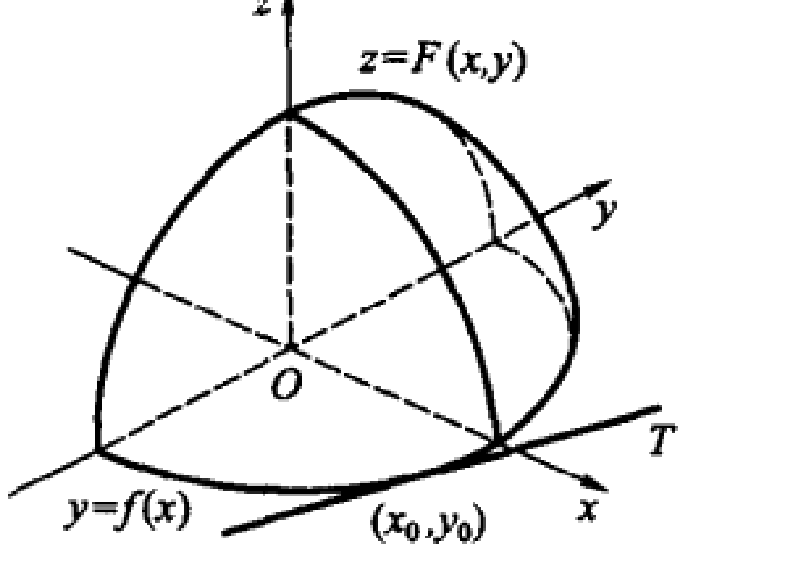
\includegraphics[width=0.45\textwidth]{work/figures/fig17-1}\caption{\relax}\label{fig:17-1}
\end{figure}

在几何上这是曲面 $z=F(x,y)$ 和坐标平面 $z=0$ 的交线．因此要使（1）式能确定隐函数，则曲面 $z=F(x,y)$ 必须与坐标面 $z=0$ 相交，也就是说，首先要存在 $P_{0}(x_{0},y_{0})$，使 $F(x_{0},y_{0})=0$．

进一步，如果希望这条过 $P_{0}$ 点的交线还是连续曲线的话，$F(x,y)$ 又应满足什么条件呢？如果曲面 $z=F(x,y)$ 在 $P_{0}$ 点有切平面，且切平面的法线不平行于 $z$ 轴，则切平面与坐标面 $z=0$ 相交为直线 $T$，这时 $z=F(x,y)$ 与 $z=0$ 必相交为曲线 $L$，且 $L$ 在 $P_{0}$ 点的切线就是 $T$．因为 $z=F(x,y)$ 在 $P_{0}$ 点的法向量为 $\left\{F_{x},F_{y},-1\right\}\big|_{P_{0}}$，所以切平面的法线不平行于 $z$ 轴意味着 $\left\{F_{x},F_{y},-1\right\}\big|_{P_{0}}$ 与 $\left\{0,0,1\right\}$ 不共线，即 $\left\{F_{x},F_{y}\right\}\big|_{P_{0}}\neq\left\{0,0\right\}$．另一方面，交线 $L$ 存在切线 $T$ 就意味着一元函数的可微性．因此条件 $\left\{F_{x},F_{y}\right\}\big|_{P_{0}}\neq\left\{0,0\right\}$ 不论对隐函数的存在性、连续性还是可微性都是重要的．下面的定理就从假定 $F_{y}\big|_{P_{0}}\neq0$ 入手．

\begin{theorem}\label{thm:17-1}
设 $F(x,y)$ 满足下列条件：

（i）$F_{x}$，$F_{y}$ 在 $D$: $\left|x-x_{0}\right|\leqslant a$，$\left|y-y_{0}\right|\leqslant b$ 上连续；

（ii）$F(x_{0},y_{0})=0$（通常称为初始条件）；

（iii）$F_{y}(x_{0},y_{0})\neq0$．

则

（1）存在 $\alpha>0$，使得在 $P_{0}$ 点的某一邻域内，方程 $F(x,y)=0$ 唯一地确定了一个定义在区间 $(x_{0}-\alpha,x_{0}+\alpha)$ 内的隐函数 $y=f(x)$，满足 $y_{0}=f(x_{0})$．换句话说，存在函数 $y=f(x)$，定义在 $(x_{0}-\alpha,x_{0}+\alpha)$ 内，满足 $F(x,f(x))\equiv0$，且 $y_{0}=f(x_{0})$；

（2）$y=f(x)$ 在 $(x_{0}-\alpha,x_{0}+\alpha)$ 连续；

（3）$y=f(x)$ 在 $(x_{0}-\alpha,x_{0}+\alpha)$ 有连续的导数，且
\[
f'(x)=-\frac{F_{x}(x,y)}{F_{y}(x,y)}.
\]
\end{theorem}

\begin{proof}
先注意一个事实，由条件（i），$F(x,y)$ 在 $D$ 上是连续的．下面分别证明各个结论成立．

由条件（iii），$F_{y}(x_{0},y_{0})\neq0$，不妨设 $F_{y}(x_{0},y_{0})>0$．又 $F_{y}(x,y)$ 在 $D$ 内连续，由连续函数的保号性，$F_{y}(x,y)$ 在 $(x_{0},y_{0})$ 点的某邻域内也大于零，为简便计，不妨设在 $D$ 上有 $F_{y}(x,y)>0$．因此对每一个 $x\in[x_{0}-a,x_{0}+a]$，$F(x,y)$ 关于 $y$ 在 $[y_{0}-b,y_{0}+b]$ 上是严格单调上升的．

固定 $x=x_{0}$，由条件（ii），$F(x_{0},y_{0})=0$ 以及 $F(x_{0},y)$ 在 $[y_{0}-b,y_{0}+b]$ 严格单调上升，知
\[
F(x_{0},y_{0}-b)<0,\ F(x_{0},y_{0}+b)>0.
\]
在 $F(x,y)$ 中分别固定 $y=y_{0}-b$ 和 $y=y_{0}+b$．由一元函数 $F(x,y_{0}-b)$，$F(x,y_{0}+b)$ 在 $x_{0}$ 连续，以及连续函数的保号性，知存在 $\alpha_{1}>0$（$\alpha_{1}<a$），使得当 $x\in(x_{0}-\alpha_{1},x_{0}+\alpha_{1})$ 时，有
\begin{equation}
F(x,y_{0}-b)<0;
\tag{2}
\end{equation}
存在 $\alpha_{2}>0$（$\alpha_{2}<a$），使得当 $x\in(x_{0}-\alpha_{2},x_{0}+\alpha_{2})$ 时，有

\begin{figure}[htbp]
\centering
\begin{tikzpicture}[scale=0.85]
% axes
\draw[-{Latex}] (-3.3,-2.1) -- (3.5,-2.1) node[below left] {$x$};
\draw[-{Latex}] (-3.3,-2.1) -- (-3.3,2.0) node[left] {$y$};
\node[below left] at (-3.3,-2.1) {$O$};
% rectangle D
\draw[thick] (-2.4,-1.5) rectangle (2.4,1.5);
% dashed guide lines: horizontal
\draw[dashed] (-3.3,1.5) -- (2.4,1.5);
\draw[dashed] (-3.3,0) -- (2.4,0);
\draw[dashed] (-3.3,-0.55) -- (2.4,-0.55);
\draw[dashed] (-3.3,-1.5) -- (2.4,-1.5);
% dashed guide lines: vertical
\draw[dashed] (-2.4,-2.1) -- (-2.4,1.5);
\draw[dashed] (-0.6,-2.1) -- (-0.6,1.5);
\draw[dashed] (0,-2.1) -- (0,1.5);
\draw[dashed] (2.4,-2.1) -- (2.4,1.5);
% inner rectangle sides x0-alpha, x0+alpha (solid, as in the book)
\draw[thick] (-1.5,-1.5) -- (-1.5,1.5);
\draw[thick] (1.7,-1.5) -- (1.7,1.5);
% curve y=f(x)
\draw[very thick] (-1.5,-0.95) .. controls (-1.05,-0.52) and (-0.9,-0.5) .. (-0.6,-0.55)
.. controls (-0.35,-0.62) and (-0.18,-0.25) .. (0,0)
.. controls (0.6,0.28) and (1.2,0.45) .. (1.7,0.55);
% labels on axes
\node[left] at (-3.3,1.5) {$y_0+b$};
\node[left] at (-3.3,0) {$y_0$};
\node[left] at (-3.3,-0.55) {$\overline{y}$};
\node[left] at (-3.3,-1.5) {$y_0-b$};
\node[below] at (-2.4,-2.15) {\scriptsize$x_0-a$};
\node[below] at (-1.5,-2.62) {\scriptsize$x_0-\alpha$};
\node[below] at (-0.6,-2.15) {\scriptsize$\overline{x}$};
\node[below] at (0,-2.62) {\scriptsize$x_0$};
\node[below] at (1.7,-2.15) {\scriptsize$x_0+\alpha$};
\node[below] at (2.4,-2.62) {\scriptsize$x_0+a$};
% point labels
\node[below right] at (-0.6,-0.55) {$\left(\overline{x},\overline{y}\right)$};
\node[above right] at (0,0) {$(x_0,y_0)$};
\node at (1.6,1.05) {$y=f(x)$};
\end{tikzpicture}\caption{\relax}\label{fig:17-2}
\end{figure}

\begin{equation}
F(x,y_{0}+b)>0.
\tag{3}
\end{equation}
令 $\alpha=\min(\alpha_{1},\alpha_{2})$，则当 $x\in(x_{0}-\alpha,x_{0}+\alpha)$ 时，（2），（3）式同时成立．

对任意 $\overline{x}\in(x_{0}-\alpha,x_{0}+\alpha)$，一元函数 $F(\overline{x},y)$ 在 $y\in[y_{0}-b,y_{0}+b]$ 连续，并且
\[
F(\overline{x},y_{0}-b)<0,\ F(\overline{x},y_{0}+b)>0.
\]
根据一元连续函数的介值定理，存在 $\overline{y}\in(y_{0}-b,y_{0}+b)$ 使得 $F(\overline{x},\overline{y})=0$，且由于 $F(\overline{x},y)$ 关于 $y$ 在 $[y_{0}-b,y_{0}+b]$ 严格单调上升，故使得 $F(\overline{x},\overline{y})=0$ 的 $\overline{y}\in(y_{0}-b,y_{0}+b)$ 是唯一的．这就确定了一个对应法则 $f$：对任意 $\overline{x}\in(x_{0}-\alpha,x_{0}+\alpha)$，都有唯一的 $\overline{y}\in(y_{0}-b,y_{0}+b)$ 与之对应，使得 $F(\overline{x},\overline{y})=0$．这就证明了，存在函数 $y=f(x)$，它定义在 $(x_{0}-\alpha,x_{0}+\alpha)$，满足 $F(x,f(x))=0$，特别地有 $y_{0}=f(x_{0})$．这样我们已经证明了结论（1）．

下面证结论（2）．既要证对任意 $\overline{x}\in(x_{0}-\alpha,x_{0}+\alpha)$，以及对任给的 $\varepsilon>0$，存在 $\delta>0$，$\delta$ 充分小使得 $(\overline{x}-\delta,\overline{x}+\delta)\subset(x_{0}-\alpha,x_{0}+\alpha)$，对任意 $x\in(\overline{x}-\delta,\overline{x}+\delta)$，有
\[
\left|f(x)-f(\overline{x})\right|<\varepsilon.
\]
任给 $\overline{x}\in(x_{0}-\alpha,x_{0}+\alpha)$，记 $\overline{y}=f(\overline{x})$．对任给的 $\varepsilon>0$，不妨设 $\varepsilon$ 充分小，使 $[\overline{y}-\varepsilon,\overline{y}+\varepsilon]\subset[y_{0}-b,y_{0}+b]$．因为 $y$ 的一元函数 $F(\overline{x},y)$ 在 $[\overline{y}-\varepsilon,\overline{y}+\varepsilon]$ 上严格单调上升，且 $F(\overline{x},\overline{y})=0$，所以
\[
F(\overline{x},\overline{y}-\varepsilon)<0,\ F(\overline{x},\overline{y}+\varepsilon)>0.
\]
而 $x$ 的一元函数 $F(x,\overline{y}-\varepsilon)$ 和 $F(x,\overline{y}+\varepsilon)$ 在 $x\in(x_{0}-\alpha,x_{0}+\alpha)$ 连续，故存在 $\delta_{1}>0$ 且 $(\overline{x}-\delta_{1},\overline{x}+\delta_{1})\subset(x_{0}-\alpha,x_{0}+\alpha)$，当 $x\in(\overline{x}-\delta_{1},\overline{x}+\delta_{1})$ 时有
\[
F(x,\overline{y}-\varepsilon)<0;
\]
存在 $\delta_{2}>0$ 且 $(\overline{x}-\delta_{2},\overline{x}+\delta_{2})\subset(x_{0}-\alpha,x_{0}+\alpha)$，当 $x\in(\overline{x}-\delta_{2},\overline{x}+\delta_{2})$ 时，有
\[
F(x,\overline{y}+\varepsilon)>0.
\]
令 $\delta=\min(\delta_{1},\delta_{2})$，则当 $x\in(\overline{x}-\delta,\overline{x}+\delta)$ 时，同时有
\[
F(x,\overline{y}-\varepsilon)<0,\ F(x,\overline{y}+\varepsilon)>0.
\]
因此只要 $x\in(\overline{x}-\delta,\overline{x}+\delta)$，$F(x,y)$ 作为 $y$ 的函数在 $(\overline{y}-\varepsilon,\overline{y}+\varepsilon)$ 就严格单调上升，且有唯一的零点 $y=f(x)$，显然满足
\[
y\in(\overline{y}-\varepsilon,\overline{y}+\varepsilon),
\]
即
\[
\left|f(x)-f(\overline{x})\right|<\varepsilon,
\]
结论（2）获证．

剩下来证明结论（3）．要证对任意 $\overline{x}\in(x_{0}-\alpha,x_{0}+\alpha)$，$y=f(x)$ 在 $\overline{x}$ 可导．令 $\left|\Delta x\right|$ 充分小使 $\overline{x}+\Delta x\in(x_{0}-\alpha,x_{0}+\alpha)$，记 $\overline{y}=f(\overline{x})$，$\overline{y}+\Delta y=f(\overline{x}+\Delta x)$．由 $y=f(x)$ 的定义知
\[
F(\overline{x},\overline{y})=0,\ F(\overline{x}+\Delta x,\overline{y}+\Delta y)=0.
\]
已知 $F(x,y)$ 在 $D$ 内有连续的偏导数，用二元函数的中值公式，存在 $\theta\in(0,1)$ 使得
\[
\begin{aligned}
0&=F(\overline{x}+\Delta x,\overline{y}+\Delta y)-F(\overline{x},\overline{y})\\
&=F_{x}(\overline{x}+\theta\Delta x,\overline{y}+\theta\Delta y)\Delta x+F_{y}(\overline{x}+\theta\Delta x,\overline{y}+\theta\Delta y)\Delta y.
\end{aligned}
\]
再由 $F_{x}$ 和 $F_{y}$ 的连续性及 $F_{y}(x,y)\neq0$，并注意到当 $\Delta x\to0$ 时 $\Delta y\to0$，便得
\[
\begin{aligned}
f'(\overline{x})&=\lim_{\Delta x\to0}\frac{\Delta y}{\Delta x}=\lim_{\Delta x\to0}-\frac{F_{x}(\overline{x}+\theta\Delta x,\overline{y}+\theta\Delta y)}{F_{y}(\overline{x}+\theta\Delta x,\overline{y}+\theta\Delta y)}\\
&=-\frac{F_{x}(\overline{x},\overline{y})}{F_{y}(\overline{x},\overline{y})}.
\end{aligned}
\]
这就是结论（3）．定理~\ref{thm:17-1} 证完．
\end{proof}

回顾定理的证明，不难看出，结论（2）的证明思路与结论（1）的证明思路完全相仿，几乎是将 $\overline{x}$，$\overline{y}$ 代替了 $x_{0}$，$y_{0}$ 后再重新叙述了一遍证明过程．其次，对于结论（1）、（2），定理条件（iii）可减弱为``$F(x,y)$ 在 $D$ 内关于 $y$ 是严格单调的''．但对结论（3），条件（iii）不能减弱．

在给出定理~\ref{thm:17-1} 之前，我们曾指出，条件 $\left\{F_{x},F_{y}\right\}\big|_{P_{0}}\neq\left\{0,0\right\}$ 不论对隐函数的存在性、连续性还是可微性都是重要的．这个条件等价于说 $F_{x}(x_{0},y_{0})\neq0$ 或 $F_{y}(x_{0},y_{0})\neq0$．考察定理~\ref{thm:17-1} 的条件，条件（i），（ii）关于 $x$，$y$ 是对称的，如果将条件（iii）改为 $F_{x}(x_{0},y_{0})\neq0$，则相应的全部结论成立，只是这时由 $F(x,y)=0$ 确定的隐函数是 $x=g(y)$．

\begin{example}\label{ex:17-1-1}
方程 $\cos y+\sin x=\mathrm{e}^{xy}$ 能否在原点的某邻域内确定隐函数 $y=f(x)$ 或 $x=g(y)$？
\end{example}

\begin{proof}[解]
令 $F(x,y)=\cos y+\sin x-\mathrm{e}^{xy}$，则
\[
F_{x}=\cos x-y\mathrm{e}^{xy},
\]
\[
F_{y}=-\sin y-x\mathrm{e}^{xy},
\]
它们都在全平面上连续，而
\[
F(0,0)=0,\ F_{x}(0,0)=1,\ F_{y}(0,0)=0,
\]
故方程在 $(0,0)$ 点的邻域内可唯一地确定可微的隐函数 $x=g(y)$，它定义在 $(-\alpha,\alpha)$，使得 $g(0)=0$，$F(g(y),y)=0$（$-\alpha<y<\alpha$）．但由于 $F_{y}(0,0)=0$，据此无法断定是否在 $(0,0)$ 点的某邻域内有隐函数 $y=f(x)$ 存在．

注意我们在这里用了``据此无法''这样的字眼，因为定理~\ref{thm:17-1} 的条件只是存在隐函数的充分条件，而不是必要条件．例如方程 $F(x,y)=y^{3}-x=0$，显然 $F_{y}(0,0)=0$，但仍可确定隐函数 $y=x^{\frac{1}{3}}$．
\end{proof}

\begin{example}\label{ex:17-1-2}
$F(x,y)=x^{2}+y^{2}-1$，$F_{x}=2x$，$F_{y}=2y$ 都在全平面连续．当 $y\neq0$ 时，$F_{y}\neq0$．由 $x^{2}+y^{2}-1=0$ 知，当 $y=0$ 时，$x=\pm1$．因此除 $(1,0)$ 和 $(-1,0)$ 点外，在单位圆上任何其它点 $(x_{0},y_{0})$，都存在 $(x_{0},y_{0})$ 的邻域，在这个邻域内可唯一确定可微的隐函数 $y=f(x)$．请读者思考，由方程可解出
\[
y=\sqrt{1-x^{2}}\quad\text{和}\quad y=-\sqrt{1-x^{2}},\ x\in(-1,1),
\]
这与隐函数存在的唯一性矛盾吗？
\end{example}

值得指出的是，定理~\ref{thm:17-1} 只肯定在 $x_{0}$ 的一个邻域，隐函数是存在的．我们说这是一个局部存在性的结果．隐函数在大范围的存在性，是个很复杂的问题，我们不在此讨论了．

现在再回头看看定理的证明，考察变量 $x$ 是否与它的维数有关．也就是说，如果将变量 $x$ 视为高维空间的点 $(x_{1},x_{2},\cdots,x_{n})$，定理的证明是否仍成立？我们发现的确成立，只要相应地把关于 $x$ 的区间改为邻域即可．

\begin{figure}[htbp]
\centering
\begin{tikzpicture}[scale=1.15]
\draw[-{Latex}] (-1.7,0) -- (1.9,0) node[below left] {$x$};
\draw[-{Latex}] (0,-1.7) -- (0,1.9) node[left] {$y$};
\node[below left] at (0,0) {$O$};
\draw[thick] (0,0) circle (1.25);
\draw (-0.35,1.08) rectangle (0.38,1.45);
\draw (-0.35,-1.45) rectangle (0.38,-1.08);
\draw (1.08,-0.35) rectangle (1.45,0.38);
\draw (-1.45,-0.35) rectangle (-1.08,0.38);
\node[right] at (0.15,1.18) {$(0,1)$};
\node[below] at (-1.25,-0.42) {$(-1,0)$};
\node[below] at (1.25,-0.42) {$(1,0)$};
\node[right] at (0.15,-1.4) {$(0,-1)$};
\end{tikzpicture}\caption{\relax}\label{fig:17-3}
\end{figure}

这样我们便可以将定理~\ref{thm:17-1} 推广到多元隐函数的情形．

\begin{theorem}\label{thm:17-2}
设函数 $F(x_{1},x_{2},\cdots,x_{n},y)$ 满足下列条件：

（i）偏导数 $F_{x_{i}}(i=1,2,\cdots,n)$ 和 $F_{y}$ 在 $D$: $\left|x_{i}-x_{i}^{(0)}\right|\leqslant a_{i}$（$i=1,2,\cdots,n$），$\left|y-y^{(0)}\right|\leqslant b$ 上连续，其中 $b>0$，$a_{i}>0$（$i=1,2,\cdots,n$）；

（ii）$F(x_{1}^{(0)},x_{2}^{(0)},\cdots,x_{n}^{(0)},y^{(0)})=0$；

（iii）$F_{y}(x_{1}^{(0)},x_{2}^{(0)},\cdots,x_{n}^{(0)},y^{(0)})\neq0$．

则

（1）存在 $Q_{0}(x_{1}^{(0)},x_{2}^{(0)},\cdots,x_{n}^{(0)})$ 的一个邻域 $O(Q_{0})$，使得在 $P_{0}(x_{1}^{(0)},x_{2}^{(0)},\cdots,x_{n}^{(0)},y^{(0)})$ 点的某邻域内，方程 $F(x_{1},x_{2},\cdots,x_{n},y)=0$ 唯一地确定了一个定义在 $O(Q_{0})$ 的 $n$ 元隐函数 $y=f(x_{1},x_{2},\cdots,x_{n})$，满足 $y^{(0)}=f(x_{1}^{(0)},x_{2}^{(0)},\cdots,x_{n}^{(0)})$．换句话说，存在函数 $y=f(x_{1},x_{2},\cdots,x_{n})$，$(x_{1},x_{2},\cdots,x_{n})\in O(Q_{0})$，使得当 $(x_{1},x_{2},\cdots,x_{n})\in O(Q_{0})$ 时，
\[
F(x_{1},x_{2},\cdots,x_{n},f(x_{1},x_{2},\cdots,x_{n}))\equiv0,
\]
且
\[
y^{(0)}=f(x_{1}^{(0)},x_{2}^{(0)},\cdots,x_{n}^{(0)});
\]

（2）$y=f(x_{1},x_{2},\cdots,x_{n})$ 在 $O(Q_{0})$ 内连续；

（3）$y=f(x_{1},x_{2},\cdots,x_{n})$ 在 $O(Q_{0})$ 内有连续的偏导数，且
\[
f_{x_{i}}=-\frac{F_{x_{i}}(x_{1},x_{2},\cdots,x_{n},y)}{F_{y}(x_{1},x_{2},\cdots,x_{n},y)},\ i=1,2,\cdots,n.
\]
\end{theorem}

\begin{example}\label{ex:17-1-3}
设 $\sin z-xyz=0$．问方程是否在原点 $(0,0,0)$ 的某邻域唯一地确定可微函数 $z=f(x,y)$，其中 $(x,y)$ 属于 $(0,0)$ 的某个邻域，使得 $\sin f(x,y)\equiv xyf(x,y)$．如可能，求 $\dfrac{\partial z}{\partial x}$，$\dfrac{\partial z}{\partial y}$．
\end{example}

\begin{proof}[解]
令 $F(x,y,z)=\sin z-xyz$．显然 $F(x,y,z)$ 在全平面有连续的偏导数，且 $F_{z}(x,y,z)=\cos z-xy$．由 $F_{z}(0,0,0)=1$，$F(0,0,0)=0$ 知，存在 $\alpha>0$，使得在 $\left|x\right|<\alpha$，$\left|y\right|<\alpha$ 有唯一的可微函数 $z=f(x,y)$，满足
\[
\sin f(x,y)=xyf(x,y),
\]
且
\[
\frac{\partial z}{\partial x}=-\frac{F_{x}(x,y,z)}{F_{z}(x,y,z)}=\frac{yz}{\cos z-xy},
\]
\[
\frac{\partial z}{\partial y}=-\frac{F_{y}(x,y,z)}{F_{z}(x,y,z)}=\frac{xz}{\cos z-xy}.
\]
\end{proof}

\begin{xiti}
\item 设函数 $F(x,y)$ 满足
\begin{ziti}
\item 在区域 $D$: $x_{0}-a\leqslant x\leqslant x_{0}+a$，$y_{0}-b\leqslant y\leqslant y_{0}+b$ 上连续；
\item $F(x_{0},y_{0})=0$；
\item 当 $x$ 固定时，函数 $F(x,y)$ 是 $y$ 的严格单调函数；
\end{ziti}
则可得到什么结论？试证明之．
\item 方程 $x^{2}+y+\sin(xy)=0$ 在原点附近能否用形如 $y=f(x)$ 的方程表示？又能否用形如 $x=g(y)$ 的方程表示？
\item 方程 $F(x,y)=y^{2}-x^{2}(1-x^{2})=0$ 在哪些点的附近可唯一地确定单值、连续、且有连续导数的函数 $y=f(x)$．
\item 证明有唯一可导的函数 $y=y(x)$ 满足方程 $\sin y+\sinh y=x$，并求出导数 $y'(x)$，其中 $\sinh y=\dfrac{\mathrm{e}^{y}-\mathrm{e}^{-y}}{2}$．
\item 方程 $xy+z\ln y+\mathrm{e}^{xz}=1$ 在点 $P_{0}(0,1,1)$ 的某邻域内能否确定出某一个变量是另外两个变量的函数．
\item 设 $f$ 是一元函数，试问 $f$ 应满足什么条件，方程
\[
2f(xy)=f(x)+f(y)
\]
在点 $(1,1)$ 的邻域内能确定出唯一的 $y$ 为 $x$ 的函数．
\item 设有方程：$x=y+\varphi(y)$，其中 $\varphi(0)=0$，且当 $-a<y<a$ 时，$\left|\varphi'(y)\right|\leqslant k<1$．证明：存在 $\delta>0$，当 $-\delta<x<\delta$ 时，存在唯一的可微函数 $y=y(x)$ 满足方程 $x=y+\varphi(y)$ 且 $y(0)=0$．
\end{xiti}

\section{方程组的情形}

关于由方程组决定的隐函数组的概念，在第十六章 §2 中已给出．下面以四个变量、两个方程的情形为例给出隐函数组存在定理．

\begin{theorem}\label{thm:17-3}
设函数 $F(x,y,u,v)$ 和 $G(x,y,u,v)$ 满足：

（i）在点 $P_{0}(x_{0},y_{0},u_{0},v_{0})$ 的某个邻域 $U$ 内，$F$，$G$ 对各变元有一阶连续偏导数；

（ii）$F(P_{0})=0$，$G(P_{0})=0$（初始条件）；

（iii）$J\big|_{P_{0}}=\dfrac{\partial(F,G)}{\partial(u,v)}\bigg|_{P_{0}}\neq0$．

则

（1）在 $P_{0}$ 点的某邻域 $\Delta\subset U$ 内，方程组
\begin{equation}
\left\{\begin{aligned}
F(x,y,u,v)&=0,\\
G(x,y,u,v)&=0
\end{aligned}\right.
\tag{1}
\end{equation}
唯一地确定一组函数 $u=u(x,y)$，$v=v(x,y)$，它们定义在 $(x_{0},y_{0})$ 的某邻域 $D$ 内，当 $(x,y)\in D$ 时，$(x,y,u,v)\in\Delta$，满足
\[
u_{0}=u(x_{0},y_{0}),\ v_{0}=v(x_{0},y_{0}),
\]
且
\[
\left\{\begin{aligned}
F(x,y,u(x,y),v(x,y))&\equiv0,\\
G(x,y,u(x,y),v(x,y))&\equiv0,
\end{aligned}\right.(x,y)\in D;
\]

（2）$u(x,y)$ 及 $v(x,y)$ 在 $D$ 内连续；

（3）$u(x,y)$ 及 $v(x,y)$ 在 $D$ 内有关于 $x$，$y$ 的连续偏导数，且
\[
\frac{\partial u}{\partial x}=-\frac{1}{J}\frac{\partial(F,G)}{\partial(x,v)},\quad \frac{\partial u}{\partial y}=-\frac{1}{J}\frac{\partial(F,G)}{\partial(y,v)},
\]
\[
\frac{\partial v}{\partial x}=-\frac{1}{J}\frac{\partial(F,G)}{\partial(u,x)},\quad \frac{\partial v}{\partial y}=-\frac{1}{J}\frac{\partial(F,G)}{\partial(u,y)}.
\]
\end{theorem}

\begin{proof}
反复应用定理~\ref{thm:17-2} 来证明．由条件（iii）
\[
\frac{\partial(F,G)}{\partial(u,v)}\bigg|_{P_{0}}=\begin{vmatrix}\dfrac{\partial F}{\partial u}&\dfrac{\partial F}{\partial v}\\[8pt]\dfrac{\partial G}{\partial u}&\dfrac{\partial G}{\partial v}\end{vmatrix}_{P_{0}}\neq0,
\]
知 $\left.\dfrac{\partial F}{\partial u}\right|_{P_{0}}$ 和 $\left.\dfrac{\partial F}{\partial v}\right|_{P_{0}}$ 至少有一个不为零，不妨设 $\left.\dfrac{\partial F}{\partial v}\right|_{P_{0}}\neq0$．由定理~\ref{thm:17-2}，方程 $F(x,y,u,v)=0$ 在 $P_{0}(x_{0},y_{0},u_{0},v_{0})$ 的某邻域内唯一地确定函数 $v=\varphi(x,y,u)$，它在 $(x_{0},y_{0},u_{0})$ 的某邻域 $V$ 内有连续的偏导数，且满足
\begin{equation}
v_{0}=\varphi(x_{0},y_{0},u_{0}),\quad F(x,y,u,\varphi(x,y,u))\equiv0.
\tag{2}
\end{equation}
记
\[
\psi(x,y,u)=G(x,y,u,\varphi(x,y,u)),\quad(x,y,u)\in V,
\]
则 $\psi(x,y,u)$ 在 $V$ 内有连续的偏导数，且 $\psi(x_{0},y_{0},u_{0})=0$．在方程组
\[
\left\{\begin{aligned}
\psi(x,y,u)&=G(x,y,u,\varphi(x,y,u)),\\
F(x,y,u,\varphi(x,y,u))&=0
\end{aligned}\right.
\]
中，两边对 $u$ 求偏导数，得
\[
\left\{\begin{aligned}
\psi_{u}&=G_{u}+G_{v}\varphi_{u},\\
F_{u}+F_{v}\varphi_{u}&=0.
\end{aligned}\right.
\]
解得
\[
\psi_{u}(x,y,u)=G_{u}-G_{v}\frac{F_{u}}{F_{v}}=-\frac{1}{F_{v}}\frac{\partial(F,G)}{\partial(u,v)}.
\]
由条件（iii）知 $\psi_{u}(x_{0},y_{0},u_{0})\neq0$，即 $\psi(x,y,u)$ 满足定理~\ref{thm:17-2} 的诸条件，从而方程
\[
G(x,y,u,\varphi(x,y,u))=0
\]
在 $(x_{0},y_{0},u_{0})$ 的某邻域内可唯一地确定函数 $u=u(x,y)$，它在 $(x_{0},y_{0})$ 的某邻域 $D$ 内有连续的偏导数，而当 $(x,y)\in D$ 时 $(x,y,u)\in V$，且满足
\[
u_{0}=u(x_{0},y_{0}),
\]
\begin{equation}
G(x,y,u(x,y)),\varphi(x,y,u(x,y))\equiv0.
\tag{3}
\end{equation}
令
\[
v(x,y)=\varphi(x,y,u(x,y)),\quad(x,y)\in D,
\]
则由（2）式知 $v(x,y)$ 在 $D$ 内有连续的偏导数，且
\begin{equation}
v_{0}=v(x_{0},y_{0}),\ F(x,y,u(x,y),v(x,y))\equiv0.
\tag{4}
\end{equation}
又由（3）式知
\begin{equation}
u_{0}=u(x_{0},y_{0}),\quad G(x,y,u(x,y),v(x,y))\equiv0,
\tag{5}
\end{equation}
即函数组 $u=u(x,y)$，$v=v(x,y)$ 就是由方程组（1）确定的满足定理要求（1）、（2）的函数组．最后只要证结论（3）中的公式成立．在（4）、（5）两式中两边对 $x$ 求偏导数，得
\[
\left\{\begin{aligned}
F_{x}+F_{u}\dfrac{\partial u}{\partial x}+F_{v}\dfrac{\partial v}{\partial x}&=0,\\[6pt]
G_{x}+G_{u}\dfrac{\partial u}{\partial x}+G_{v}\dfrac{\partial v}{\partial x}&=0.
\end{aligned}\right.
\]
用克拉默法则解出 $\dfrac{\partial u}{\partial x}$，$\dfrac{\partial v}{\partial x}$，即得
\[
\frac{\partial u}{\partial x}=-\frac{1}{J}\frac{\partial(F,G)}{\partial(x,v)},\quad \frac{\partial v}{\partial x}=-\frac{1}{J}\frac{\partial(F,G)}{\partial(u,x)}.
\]
同理在（4）、（5）两式中两边对 $y$ 求偏导数，得
\[
\frac{\partial u}{\partial y}=-\frac{1}{J}\frac{\partial(F,G)}{\partial(y,v)},\quad \frac{\partial v}{\partial y}=-\frac{1}{J}\frac{\partial(F,G)}{\partial(u,y)}.
\]
定理~\ref{thm:17-3} 证完．
\end{proof}

从定理~\ref{thm:17-3} 的证明中可见，条件（iii）在定理中的地位和作用与定理~\ref{thm:17-1} 中的条件 $F_{y}(x_{0},y_{0})\neq0$ 的地位和作用相当，它对于隐函数组的存在性、连续性和可微性都是重要的．另外，结论（3）中公式的推导方法就是我们在第十六章 §2 中介绍的隐函数组求导法，因此公式不必死记硬背，重要的是掌握求导方法．

\begin{example}\label{ex:17-2-1}
设有方程组
\[
\left\{\begin{aligned}
F(x,y,u,v)&=u^{2}+v^{2}-x^{2}-y=0,\\
G(x,y,u,v)&=-u+v-xy+1=0.
\end{aligned}\right.
\]
讨论在 $P_{0}(2,1,1,2)$ 的某邻域能否确定隐函数组 $u=u(x,y)$，$v=v(x,y)$．又问在 $P_{0}$ 点的某邻域能否确定函数组 $x=x(u,y)$，$v=v(u,y)$．对确定的函数组求其偏导数．
\end{example}

\begin{proof}[解]
显然 $F$，$G$ 在全平面上有连续的偏导数．又
\[
\begin{pmatrix}F_{x}&F_{y}&F_{u}&F_{v}\\ G_{x}&G_{y}&G_{u}&G_{v}\end{pmatrix}=\begin{pmatrix}-2x&-1&2u&2v\\ -y&-x&-1&1\end{pmatrix},
\]
\[
F(2,1,1,2)=0,\ G(2,1,1,2)=0,
\]
\[
\frac{\partial(F,G)}{\partial(u,v)}\bigg|_{P_{0}}=\begin{vmatrix}2u&2v\\ -1&1\end{vmatrix}_{P_{0}}=6\neq0,
\]
\[
\frac{\partial(F,G)}{\partial(x,v)}\bigg|_{P_{0}}=\begin{vmatrix}-2x&2v\\ -y&1\end{vmatrix}_{P_{0}}=0,
\]
因此在 $P_{0}$ 点的某邻域方程组可以唯一地确定一组可微函数 $u=u(x,y)$，$v=v(x,y)$，但在 $P_{0}$ 点的附近难以断言是否可唯一确定函数组 $x=x(u,y)$，$v=v(u,y)$．为求函数 $u(x,y)$ 和 $v(x,y)$ 的偏导数，在方程组两边对 $x$ 求偏导数，得
\[
\left\{\begin{aligned}
2u\frac{\partial u}{\partial x}+2v\frac{\partial v}{\partial x}-2x&=0,\\
-\frac{\partial u}{\partial x}+\frac{\partial v}{\partial x}-y&=0,
\end{aligned}\right.
\]
解得
\[
\frac{\partial u}{\partial x}=\frac{x-yv}{u+v},\quad \frac{\partial v}{\partial x}=\frac{yu+x}{u+v}.
\]
在方程组两边对 $y$ 求偏导数得
\[
\left\{\begin{aligned}
2u\frac{\partial u}{\partial y}+2v\frac{\partial v}{\partial y}-1&=0,\\
-\frac{\partial u}{\partial y}+\frac{\partial v}{\partial y}-x&=0,
\end{aligned}\right.
\]
解得
\[
\frac{\partial u}{\partial y}=\frac{1-2xv}{2(u+v)},\quad \frac{\partial v}{\partial y}=\frac{2xu+1}{2(u+v)}.
\]
\end{proof}

作为定理~\ref{thm:17-3} 的应用，我们考虑反函数组．

设有定义在平面点集 $D$ 上的函数组
\begin{equation}
u=u(x,y),\ v=v(x,y),\ (x,y)\in D,
\tag{6}
\end{equation}
则对于任意点 $(x,y)\in D$，都有平面上唯一的点 $(u,v)$ 与之对应．记 $D$ 的所有对应点的集合为 $D'$，即
\[
D'=\left\{(u,v)\mid(u,v)=(u(x,y),v(x,y)),\ (x,y)\in D\right\}.
\]
若反过来，对于任意点 $(u,v)\in D'$，都有唯一的点 $(x,y)\in D$，使得（6）式成立，也就是说，这时可确定两个定义在 $D'$ 上的函数
\begin{equation}
x=x(u,v),\ y=y(u,v),
\tag{7}
\end{equation}
在 $D'$ 上满足恒等式
\[
u\equiv u(x(u,v),y(u,v)),\quad v\equiv v(x(u,v),y(u,v)).
\]
则称函数组（7）是函数组（6）的反函数组．

上述对应关系可以用映射的语言加以叙述．我们称由（6）式给出的从 $D$ 到 $D'$ 的对应为映射 $T$：$D\to D'$，它把任意的 $(x,y)\in D$ 映为 $T(x,y)=(u,v)\in D'$．$D'$ 是 $D$ 在映射 $T$ 下的像集，记为 $D'=T(D)$．而（7）式则给出了从 $D'$ 到 $D$ 的映射 $T'$，它是 $T$ 的逆映射，即如果对任意的 $(u,v)\in D'$，有唯一的 $(x,y)\in D$，使得 $T(x,y)=(u,v)$，则说 $T'(u,v)=(x,y)$．这样的 $T'$ 存在的条件是：若 $(x_{1},y_{1}),(x_{2},y_{2})\in D$，且 $(x_{1},y_{1})\neq(x_{2},y_{2})$，则
\[
T(x_{1},y_{1})=(u_{1},v_{1})\neq T(x_{2},y_{2})=(u_{2},v_{2}).
\]
也就是说，$D$ 和 $D'$ 是一一对应的．$T$ 把 $D$ 映成 $D'$，而依同一关系，$T'$ 把 $D'$ 映回 $D$．这时记 $T'$ 为 $T^{-1}$．显然
\[
T^{-1}(T(x,y))=T^{-1}(u,v)=(x,y),\ (x,y)\in D,
\]
\[
T(T^{-1}(u,v))=T(x,y)=(u,v),\ (u,v)\in D'.
\]
因此，若 $T^{-1}$ 是 $T$ 的逆映射，则 $T$ 是 $T^{-1}$ 的逆映射．即 $T$ 与 $T^{-1}$ 互为逆映射．也就是说（6）、（7）式给出的函数组互为反函数组．

令
\[
\left\{\begin{aligned}
F(x,y,u,v)&=u-u(x,y)=0,\\
G(x,y,u,v)&=v-v(x,y)=0,
\end{aligned}\right.
\]
对 $F$ 和 $G$ 用定理~\ref{thm:17-3}，便得下面的反函数组定理．

\begin{theorem}\label{thm:17-4}
设函数组（6）满足

（i）在 $P_{0}(x_{0},y_{0})$ 的某邻域 $D$ 内对 $x$，$y$ 有连续偏导数；

（ii）$u_{0}=u(x_{0},y_{0})$，$v_{0}=v(x_{0},y_{0})$；

（iii）$\dfrac{\partial(u,v)}{\partial(x,y)}\bigg|_{(x_{0},y_{0})}\neq0$．

则在 $Q_{0}(u_{0},v_{0})$ 的某邻域 $D'$ 内存在唯一的一组反函数 $x=x(u,v)$，$y=y(u,v)$ 使得

（1）$x_{0}=x(u_{0},v_{0})$，$y_{0}=y(u_{0},v_{0})$，且当 $(u,v)\in D'$ 时 $(x,y)\in D$，有
\[
u\equiv u(x(u,v),y(u,v)),
\]
\[
v\equiv v(x(u,v),y(u,v));
\]

（2）$x(u,v)$，$y(u,v)$ 在 $D'$ 内存在连续的一阶偏导数，且
\[
\frac{\partial x}{\partial u}=\frac{1}{J}\frac{\partial v}{\partial y},\quad \frac{\partial x}{\partial v}=-\frac{1}{J}\frac{\partial u}{\partial y},
\]
\[
\frac{\partial y}{\partial u}=-\frac{1}{J}\frac{\partial v}{\partial x},\quad \frac{\partial y}{\partial v}=\frac{1}{J}\frac{\partial u}{\partial x}.
\]
其中 $J=\dfrac{\partial(u,v)}{\partial(x,y)}$．
\end{theorem}

\begin{corollary}\label{cor:17-1}
在定理~\ref{thm:17-4} 的条件下有 $\dfrac{\partial(x,y)}{\partial(u,v)}\cdot\dfrac{\partial(u,v)}{\partial(x,y)}=1$．
\end{corollary}

\begin{proof}
由定理~\ref{thm:17-4} 的结论（2）有
\[
\begin{aligned}
\frac{\partial(x,y)}{\partial(u,v)}&=\begin{vmatrix}\dfrac{\partial x}{\partial u}&\dfrac{\partial x}{\partial v}\\[8pt]\dfrac{\partial y}{\partial u}&\dfrac{\partial y}{\partial v}\end{vmatrix}=\frac{1}{J^{2}}\begin{vmatrix}\dfrac{\partial v}{\partial y}&-\dfrac{\partial u}{\partial y}\\[8pt]-\dfrac{\partial v}{\partial x}&\dfrac{\partial u}{\partial x}\end{vmatrix}\\
&=\frac{1}{J^{2}}\begin{vmatrix}\dfrac{\partial u}{\partial x}&\dfrac{\partial u}{\partial y}\\[8pt]\dfrac{\partial v}{\partial x}&\dfrac{\partial v}{\partial y}\end{vmatrix}=\frac{1}{J},
\end{aligned}
\]
即
\[
\frac{\partial(x,y)}{\partial(u,v)}\cdot J=\frac{\partial(x,y)}{\partial(u,v)}\cdot\frac{\partial(u,v)}{\partial(x,y)}=1.
\]
推论~\ref{cor:17-1} 证完．
\end{proof}

推论~\ref{cor:17-1} 可视为一元反函数导数公式 $\dfrac{\dd y}{\dd x}\cdot\dfrac{\dd x}{\dd y}=1$ 的推广．

\begin{corollary}\label{cor:17-2}
设函数组 $u=u(x,y)$，$v=v(x,y)$ 在开集 $D$ 内有连续偏导数，且在 $D$ 内 $\dfrac{\partial(u,v)}{\partial(x,y)}$ 恒不为零，则由函数组定义的映射 $T:D\to T(D)$ 的像集 $T(D)$ 是 $uv$ 平面上的开集．
\end{corollary}

\begin{proof}
对任意 $Q_{0}(u_{0},v_{0})\in T(D)$，设 $Q_{0}$ 是 $P_{0}(x_{0},y_{0})$ 在映射 $T$ 下的像，即 $u_{0}=u(x_{0},y_{0})$，$v_{0}=v(x_{0},y_{0})$．由反函数组定理，在 $Q_{0}$ 点的某邻域 $O(Q_{0})$ 内，存在唯一的一组反函数 $x=x(u,v)$，$y=y(u,v)$，使得 $x_{0}=x(u_{0},v_{0})$，$y_{0}=y(u_{0},v_{0})$，当 $(u,v)\in O(Q_{0})$ 时，$(x,y)\in D$，且有恒等式
\[
u\equiv u(x(u,v),y(u,v)),\quad v=v(x(u,v),y(u,v)).
\]
即 $O(Q_{0})$ 内的每一点都是 $D$ 中某一点的像，故 $O(Q_{0})\subset T(D)$．这就证明了 $T(D)$ 是开集．推论~\ref{cor:17-2} 证完．
\end{proof}

\begin{corollary}\label{cor:17-3}
在推论~\ref{cor:17-2} 的条件下，设 $E\subset D$ 是任一有界闭集，则它的像集 $T(E)$（$\subset T(D)$）也是有界闭集，且 $E$ 的内点映射为 $T(E)$ 的内点，$E$ 的边界点映射为 $T(E)$ 的边界点．
\end{corollary}

\begin{proof}
由于 $u(x,y)$ 和 $v(x,y)$ 在有界闭集上连续，从而有界，即 $T(E)$ 是有界集．下证 $T(E)$ 是闭集．设 $(u_{0},v_{0})$ 是 $T(E)$ 的聚点，则存在 $T(E)$ 中异于 $(u_{0},v_{0})$ 的点列 $\{(u_{n},v_{n})\}$，使得 $\lim\limits_{n\to\infty}(u_{n},v_{n})=(u_{0},v_{0})$．即存在 $E$ 中的点列 $\{(x_{n},y_{n})\}$，使得
\[
u_{n}=u(x_{n},y_{n}),\ v_{n}=v(x_{n},y_{n}),\ n=1,2,\cdots,
\]
且
\[
\lim_{n\to\infty}(u_{n},v_{n})=\lim_{n\to\infty}\left(u(x_{n},y_{n}),v(x_{n},y_{n})\right)=(u_{0},v_{0}).
\]
由致密性定理知 $\{(x_{n},y_{n})\}$ 有收敛子列 $\{(x_{n_{k}},y_{n_{k}})\}$．记其极限为 $(x_{0},y_{0})$，则有
\[
\lim_{k\to\infty}(x_{n_{k}},y_{n_{k}})=(x_{0},y_{0}).
\]
由 $E$ 闭知 $(x_{0},y_{0})\in E$，而函数 $u(x,y)$ 和 $v(x,y)$ 在 $E$ 上连续，所以
\[
\begin{aligned}
(u_{0},v_{0})&=\lim_{k\to\infty}\left(u(x_{n_{k}},y_{n_{k}}),v(x_{n_{k}},y_{n_{k}})\right)\\
&=\left(u(x_{0},y_{0}),v(x_{0},y_{0})\right).
\end{aligned}
\]
这表明 $(u_{0},v_{0})\in T(E)$，即 $T(E)$ 是闭集．

对 $T$ 用推论~\ref{cor:17-2}，知 $T$ 将 $E$ 的内点映射为 $T(E)$ 的内点．若 $T$ 将 $E$ 的某个边界点 $(x',y')$ 映射为 $T(E)$ 的内点 $(u',v')$，由定理~\ref{thm:17-4} 及推论~\ref{cor:17-1} 知，在 $(u',v')$ 的某邻域内存在 $T^{-1}$ 满足推论~\ref{cor:17-2} 的条件，于是 $T^{-1}$ 将 $(u',v')$ 映射为 $E$ 的内点 $(x',y')$，这与 $(x',y')$ 是 $E$ 的边界点矛盾，故 $(u',v')$ 是 $T(E)$ 的边界点．推论~\ref{cor:17-3} 证完．
\end{proof}

\begin{example}\label{ex:17-2-2}
极坐标与直角坐标的变换为
\[
x=r\cos\theta,\quad y=r\sin\theta.
\]
因为
\[
\frac{\partial(x,y)}{\partial(r,\theta)}=\begin{vmatrix}\dfrac{\partial x}{\partial r}&\dfrac{\partial x}{\partial\theta}\\[8pt]\dfrac{\partial y}{\partial r}&\dfrac{\partial y}{\partial\theta}\end{vmatrix}=\begin{vmatrix}\cos\theta&-r\sin\theta\\ \sin\theta&r\cos\theta\end{vmatrix}=r,
\]
所以除 $r=0$ 即坐标原点 $(0,0)$ 外，变换的逆变换存在，即有
\[
r=r(x,y),\ \theta=\theta(x,y).
\]
且
\[
\frac{\partial(r,\theta)}{\partial(x,y)}=\frac{1}{\dfrac{\partial(x,y)}{\partial(r,\theta)}}=\frac{1}{r}.
\]
\end{example}

最后，我们将定理~\ref{thm:17-3} 推广到一般的情形，即 $n+m$ 个变量，$n$ 个方程的情形．

\begin{theorem}\label{thm:17-5}
设有 $n$ 个 $n+m$ 元函数 $F_{i}(x_{1},x_{2},\cdots,x_{m},y_{1},y_{2},\cdots,y_{n})$（$i=1,2,\cdots,n$），满足

（i）在点 $P_{0}(x_{1}^{(0)},\cdots,x_{m}^{(0)},y_{1}^{(0)},\cdots,y_{n}^{(0)})$ 的某邻域 $U$ 内有对各变元的连续偏导数；

（ii）$F_{i}(P_{0})=0$，$i=1,2,\cdots,n$；

（iii）$J=\dfrac{\partial(F_{1},F_{2},\cdots,F_{n})}{\partial(y_{1},y_{2},\cdots,y_{n})}\bigg|_{P_{0}}\neq0$．

则（1）在 $P_{0}$ 的某邻域内，方程组
\[
F_{i}(x_{1},\cdots,x_{m},y_{1},\cdots,y_{n})=0\quad(i=1,2,\cdots,n)
\]
唯一地确定函数组
\[
y_{i}=f_{i}(x_{1},x_{2},\cdots,x_{m})\quad(i=1,2,\cdots,n),
\]
它们定义在 $(x_{1}^{(0)},x_{2}^{(0)},\cdots,x_{m}^{(0)})$ 的某邻域 $D$ 内，使得
\[
y_{i}^{(0)}=f_{i}(x_{1}^{(0)},x_{2}^{(0)},\cdots,x_{m}^{(0)})\quad(i=1,2,\cdots,n),
\]
且当 $(x_{1},x_{2},\cdots,x_{m})\in D$ 时有恒等式
\[
F_{i}(x_{1},x_{2},\cdots,x_{m},f_{1}(x_{1},x_{2},\cdots,x_{m}),\cdots,f_{n}(x_{1},x_{2},\cdots,x_{m}))\equiv0;
\]

（2）这组函数 $f_{i}$（$i=1,2,\cdots,n$）在 $D$ 内连续；

（3）这组函数 $f_{i}$（$i=1,2,\cdots,n$）在 $D$ 内对各变元有连续的偏导数，且对 $x_{j}$（$j=1,2,\cdots,n$）的偏导数可由下面方程组解出．
\[
\frac{\partial F_{i}}{\partial x_{j}}+\frac{\partial F_{i}}{\partial y_{1}}\frac{\partial f_{1}}{\partial x_{j}}+\frac{\partial F_{i}}{\partial y_{2}}\frac{\partial f_{2}}{\partial x_{j}}+\cdots+\frac{\partial F_{i}}{\partial y_{n}}\frac{\partial f_{n}}{\partial x_{j}}=0,\ i=1,2,\cdots,n.
\]
\end{theorem}

\begin{example}\label{ex:17-2-3}
点 $(1,-1,2)$ 在方程 $x^{2}(y^{2}+z^{2})=5$ 及 $(x-z)^{2}+y^{2}=2$ 所表示的曲面上，证明在这点的一个邻域内，两曲面的交线能用形如 $z=f(x)$，$y=g(x)$ 的一对方程表示．并求 $\dfrac{\dd z}{\dd x}$ 和 $\dfrac{\dd y}{\dd x}$．
\end{example}

\begin{proof}[证明]
令
\[
\left\{\begin{aligned}
F(x,y,z)&=x^{2}(y^{2}+z^{2})-5,\\
G(x,y,z)&=(x-z)^{2}+y^{2}-2,
\end{aligned}\right.
\]
这时 $F(1,-1,2)=0$，$G(1,-1,2)=0$．显然 $F$，$G$ 在点 $P_{0}(1,-1,2)$ 的任何邻域内有连续的偏导数，且
\[
\begin{aligned}
\left.\frac{\partial(F,G)}{\partial(y,z)}\right|_{P_{0}}&=\begin{vmatrix}\dfrac{\partial F}{\partial y}&\dfrac{\partial F}{\partial z}\\[8pt]\dfrac{\partial G}{\partial y}&\dfrac{\partial G}{\partial z}\end{vmatrix}_{P_{0}}=\begin{vmatrix}2x^{2}y&2x^{2}z\\ 2y&-2(x-z)\end{vmatrix}_{P_{0}}\\
&=\begin{vmatrix}-2&4\\ -2&2\end{vmatrix}=4\neq0.
\end{aligned}
\]
由定理~\ref{thm:17-5}，在 $P_{0}$ 点的某邻域内可唯一确定隐函数组
\[
z=f(x),\quad y=g(x),
\]
它们定义在 $x_{0}=1$ 点的某邻域内，使得 $f(1)=2$，$g(1)=-1$ 且
\[
F(x,g(x),f(x))\equiv0,\quad G(x,g(x),f(x))\equiv0.
\]
这表明两曲面的交线在 $P_{0}$ 附近能用形如 $z=f(x)$，$y=g(x)$ 的一对方程表示．在方程组两边对 $x$ 求导得
\[
\left\{\begin{aligned}
2x(y^{2}+z^{2})+x^{2}(2yy'+2zz')&=0,\\
2(x-z)(1-z')+2yy'&=0,
\end{aligned}\right.
\]
即
\[
\left\{\begin{aligned}
x^{2}yy'+x^{2}zz'&=-x(y^{2}+z^{2}),\\
yy'-(x-z)z'&=-(x-z).
\end{aligned}\right.
\]
解这个关于 $y'$ 和 $z'$ 的线性方程组得
\[
y'=\frac{y^{2}z-xy^{2}+z^{3}-x^{2}z}{x^{2}y},
\]
\[
z'=\frac{x^{2}-xz-y^{2}-z^{2}}{x^{2}}.
\]
\end{proof}

\begin{xiti}
\item 试讨论方程组
\[
\left\{\begin{aligned}
x^{2}+y^{2}&=\dfrac{1}{2}z^{2},\\
x+y+z&=2
\end{aligned}\right.
\]
在点 $P_{0}(1,-1,2)$ 的附近能否确定形如 $x=f(z)$，$y=g(z)$ 的隐函数组．
\item 求下列函数组的反函数组的偏导数：
\begin{ziti}
\item 设 $u=x\cos\dfrac{y}{x}$，$v=x\sin\dfrac{y}{x}$，求 $\dfrac{\partial x}{\partial u}$，$\dfrac{\partial x}{\partial v}$，$\dfrac{\partial y}{\partial u}$，$\dfrac{\partial y}{\partial v}$；
\item 设 $u=\mathrm{e}^{x}+x\sin y$，$v=\mathrm{e}^{x}-x\cos y$，求 $\dfrac{\partial x}{\partial u}$，$\dfrac{\partial x}{\partial v}$，$\dfrac{\partial y}{\partial u}$，$\dfrac{\partial y}{\partial v}$．
\end{ziti}
\item 设 $u=\dfrac{x}{r^{2}}$，$v=\dfrac{y}{r^{2}}$，$w=\dfrac{z}{r^{2}}$，其中 $r=\sqrt{x^{2}+y^{2}+z^{2}}$．
\begin{ziti}
\item 试求以 $u,v,w$ 为自变量的反函数组；
\item 计算 $\dfrac{\partial(u,v,w)}{\partial(x,y,z)}$．
\end{ziti}
\item 设 $f_{i}$，$\varphi_{i}$ 连续可微，且
\[
F_{i}(x_{1},\cdots,x_{n})=f_{i}(\varphi_{1}(x_{1}),\varphi_{2}(x_{2}),\cdots,\varphi_{n}(x_{n}))\quad(i=1,2,\cdots,n).
\]
求 $\dfrac{\partial(F_{1},F_{2},\cdots,F_{n})}{\partial(x_{1},x_{2},\cdots,x_{n})}$．
\item 据理说明：在点 $(0,1)$ 附近是否存在连续可微函数 $f(x,y)$ 和 $g(x,y)$ 满足 $f(0,1)=1$，$g(0,1)=-1$，且
\[
\begin{aligned}
&\left[f(x,y)\right]^{3}+xg(x,y)-y=0,\\
&\left[g(x,y)\right]^{3}+yf(x,y)-x=0.
\end{aligned}
\]
\item 设
\[
\left\{\begin{aligned}
u&=f(x,y,z,t),\\
g(y,z,t)&=0,\\
h(z,t)&=0.
\end{aligned}\right.
\]
在什么条件下 $u$ 是 $x$，$y$ 的函数？求 $\dfrac{\partial u}{\partial x}$，$\dfrac{\partial u}{\partial y}$．
\item 设函数 $u=u(x)$ 由方程组
\[
\left\{\begin{aligned}
u&=f(x,y,z),\\
g(x,y,z)&=0,\\
h(x,y,z)&=0
\end{aligned}\right.
\]
所确定，求 $\dfrac{\dd u}{\dd x}$，$\dfrac{\dd^{2}u}{\dd x^{2}}$．
\item 设 $z=z(x,y)$ 满足方程组
\[
\left\{\begin{aligned}
f(x,y,z,t)&=0,\\
g(x,y,z,t)&=0.
\end{aligned}\right.
\]
求 $\dd z$．
\item 设
\[
\left\{\begin{aligned}
u&=f(x-ut,y-ut,z-ut),\\
g(x,y,z)&=0.
\end{aligned}\right.
\]
求 $\dfrac{\partial u}{\partial x}$，$\dfrac{\partial u}{\partial y}$．这时 $t$ 是自变量还是因变量？
\item 设 $(x_{0},y_{0},z_{0},u_{0})$ 满足方程组
\[
\left\{\begin{aligned}
f(x)+f(y)+f(z)&=F(u),\\
g(x)+g(y)+g(z)&=G(u),\\
h(x)+h(y)+h(z)&=H(u),
\end{aligned}\right.
\]
这里所有的函数假定有连续的导数．
\begin{ziti}
\item 说出一个能在该点邻域内确定 $x$，$y$，$z$ 作为 $u$ 的函数的充分条件；
\item 在 $f(x)=x$，$g(x)=x^{2}$，$h(x)=x^{3}$ 的情形下，上述条件相当于什么？
\end{ziti}
\item 设 $x=u$，$y=\dfrac{u}{1+uv}$，$z=\dfrac{u}{1+uw}$，取 $u$，$v$ 为新的自变量，$w$ 为新的因变量，变换方程
\[
x^{2}\frac{\partial z}{\partial x}+y^{2}\frac{\partial z}{\partial y}=z^{2}.
\]
\end{xiti}

% !TeX program = xelatex
% 第十八章 极值与条件极值
\chapter{极值与条件极值}

本章讨论多元微分学的重要应用——多元函数的极值．回忆一元函数的极值问题，求解的基本思想是分两步走．第一步从函数定义域中确定出可能的极值点，第二步是判别这些可能的极值点是否确是极值点．为此，我们需要函数取极值的必要条件和充分条件．必要条件可以使我们实现第一步，而充分条件则可以实现第二步．对于多元函数的极值问题，我们仍然是按这样一条思路去做，分别给出函数取极值的必要条件和充分条件．不过对充分条件的讨论，多元函数情形要比一元函数情形复杂得多．

求条件极值的拉格朗日乘数法将条件极值完全化为了无条件极值，大大地简化了计算．

\section{极值与最小二乘法}

\subsection{多元函数的极值}

以二元函数为例进行讨论．

\begin{definition}\label{def:18-1}
设函数 $f(x,y)$ 在点 $P_{0}(x_{0},y_{0})$ 的某邻域 $O(P_{0})$ 内有定义．若对于任意点 $P(x,y)\in O(P_{0})$，有
\begin{equation}
f(P)\leqslant f(P_{0}),
\tag{1}
\end{equation}
则称函数 $f(x,y)$ 在 $P_{0}$ 点取极大值，点 $P_{0}$ 称为 $f$ 的极大值点．若对于任意点 $P\in O(P_{0})$，有 $f(P)\geqslant f(P_{0})$，则称函数 $f(x,y)$ 在 $P_{0}$ 取极小值，点 $P_{0}$ 称为 $f$ 的极小值点．
\end{definition}

极大值和极小值统称为极值．极大值点和极小值点统称为极值点．

从定义中易见，若 $P_{0}(x_{0},y_{0})$ 是 $f(x,y)$ 的极值点，则 $x_{0}$ 是一元函数 $f(x,y_{0})$ 的极值点，$y_{0}$ 是一元函数 $f(x_{0},y)$ 的极值点．而在 $P_{0}$ 点函数 $f(x,y)$ 的偏导数可能存在，也可能不存在．若是前者，则由一元函数取极值的必要条件便知，$f_{x}(x_{0},y_{0})=f_{y}(x_{0},y_{0})=0$．把这写成下面的定理．

\begin{theorem}[取极值的必要条件]\label{thm:18-1}
设函数 $f(x,y)$ 在点 $P_{0}(x_{0},y_{0})$ 存在对各变元的偏导数，且 $P_{0}$ 是极值点，则有
\begin{equation}
f_{x}(P_{0})=0,\quad f_{y}(P_{0})=0.
\tag{2}
\end{equation}
\end{theorem}

满足（2）式的点称为函数的稳定点．由定理 18.1 知，极值点要么是稳定点，要么在其上至少有一个偏导数不存在．

例如锥面 $z=\sqrt{x^{2}+y^{2}}$，显然它在点 $(0,0)$ 取得最小值，但在点 $(0,0)$ 两个偏导数 $z_{x}(0,0)$ 和 $z_{y}(0,0)$ 都不存在．参见图~\ref{fig:18-1}．

注意：定理 18.1 仅是取极值的必要条件，不是充分条件．例如马鞍面 $z=xy$ 在点 $(0,0)$ 有 $z_{x}(0,0)=z_{y}(0,0)=0$，但显然 $(0,0)$ 点不是极值点．事实上，在 $(0,0)$ 点的任何邻域内都存在两点其函数值异号，而 $z(0,0)=0$（见图~\ref{fig:18-2}）．

\begin{figure}[htbp]
\centering
\begin{minipage}[c]{0.42\textwidth}\centering
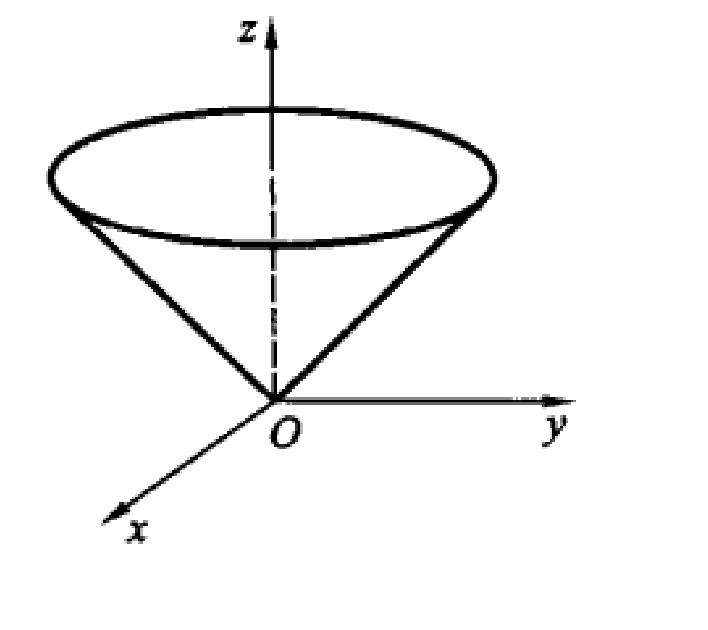
\includegraphics[width=0.86\textwidth]{work/figures/fig18-1}\caption{\relax}\label{fig:18-1}
\end{minipage}\hfill
\begin{minipage}[c]{0.55\textwidth}\centering
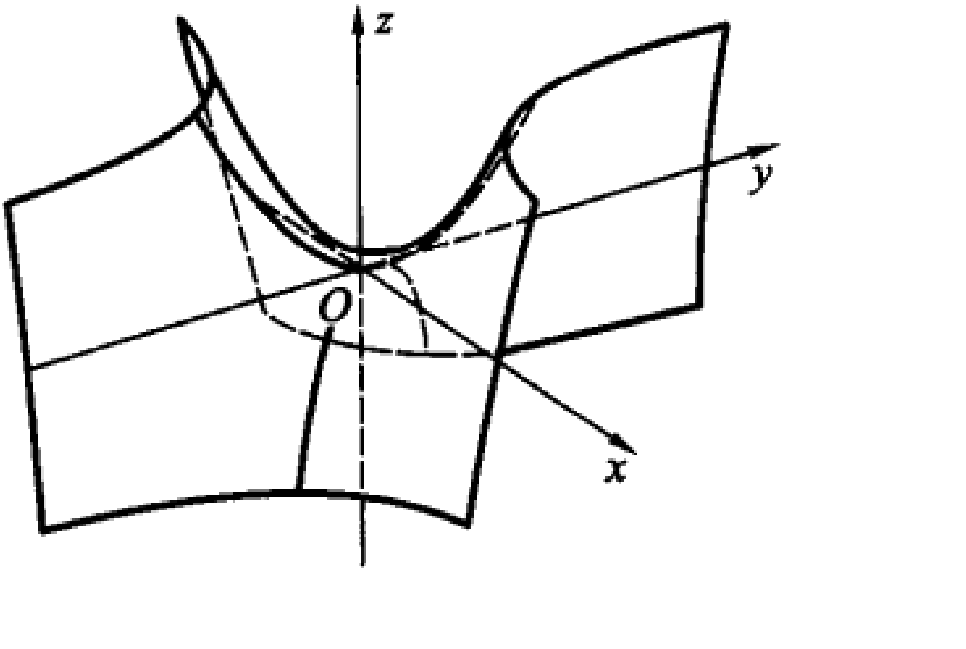
\includegraphics[width=0.98\textwidth]{work/figures/fig18-2}\caption{\relax}\label{fig:18-2}
\end{minipage}
\end{figure}

下面讨论取极值的充分条件，用来判别稳定点是否确是极值点．类似于一元函数的情形，我们用泰勒公式进行讨论．

设 $f(x,y)$ 在 $(x_{0},y_{0})$ 具有二阶连续偏导数．记
\[
a_{11}=f_{xx}(x_{0},y_{0}),\quad a_{12}=f_{xy}(x_{0},y_{0}),\quad a_{22}=f_{yy}(x_{0},y_{0}),
\]
\[
D=\left|\begin{array}{cc}a_{11}&a_{12}\\ a_{12}&a_{22}\end{array}\right|=a_{11}a_{22}-a_{12}^{2}.
\]

\begin{theorem}\label{thm:18-2}
如果 $f(x,y)$ 在 $P_{0}(x_{0},y_{0})$ 的某邻域内具有二阶的连续偏导数，$f_{x}(x_{0},y_{0})=0$，$f_{y}(x_{0},y_{0})=0$，那么

（i）若 $D>0$，则当 $a_{11}>0$（或 $a_{22}>0$）时，$f$ 在 $P_{0}$ 取极小值；当 $a_{11}<0$（或 $a_{22}<0$）时，$f$ 在 $P_{0}$ 取极大值．

（ii）若 $D<0$，则 $P_{0}$ 不是 $f$ 的极值点．

（iii）若 $D=0$，则不能判定 $f$ 在 $P_{0}$ 是否取极值，需进一步讨论．
\end{theorem}

\begin{proof}
用二元函数的泰勒公式，并注意到 $f_{x}(x_{0},y_{0})=0$，$f_{y}(x_{0},y_{0})=0$，则有
\[
\begin{aligned}
\Delta f&=f(x_{0}+\Delta x,y_{0}+\Delta y)-f(x_{0},y_{0})\\
&=\frac{1}{2}\left\{f_{xx}(x_{0}+\theta\Delta x,y_{0}+\theta\Delta y)\Delta x^{2}+2f_{xy}(x_{0}+\theta\Delta x,y_{0}+\theta\Delta y)\Delta x\Delta y+\right.\\
&\quad\left.f_{yy}(x_{0}+\theta\Delta x,y_{0}+\theta\Delta y)\Delta y^{2}\right\}\\
&=\frac{1}{2}\left\{f_{xx}(x_{0},y_{0})\Delta x^{2}+2f_{xy}(x_{0},y_{0})\Delta x\Delta y+f_{yy}(x_{0},y_{0})\Delta y^{2}+\right.\\
&\quad\left.\alpha_{11}\Delta x^{2}+2\alpha_{12}\Delta x\Delta y+\alpha_{22}\Delta y^{2}\right\}\\
&=\frac{1}{2}\left\{a_{11}\Delta x^{2}+2a_{12}\Delta x\Delta y+a_{22}\Delta y^{2}+\alpha_{11}\Delta x^{2}+2\alpha_{12}\Delta x\Delta y+\alpha_{22}\Delta y^{2}\right\},
\end{aligned}
\]
其中当 $\Delta x\to0$，$\Delta y\to0$ 时，
\[
\begin{aligned}
\alpha_{11}&=f_{xx}(x_{0}+\theta\Delta x,y_{0}+\theta\Delta y)-f_{xx}(x_{0},y_{0})\to0,\\
\alpha_{12}&=f_{xy}(x_{0}+\theta\Delta x,y_{0}+\theta\Delta y)-f_{xy}(x_{0},y_{0})\to0,\\
\alpha_{22}&=f_{yy}(x_{0}+\theta\Delta x,y_{0}+\theta\Delta y)-f_{yy}(x_{0},y_{0})\to0.
\end{aligned}
\]
为讨论方便，令 $\Delta x=\rho\cos\varphi$，$\Delta y=\rho\sin\varphi$，则
\[
\begin{aligned}
\Delta f&=\frac{\rho^{2}}{2}\left[a_{11}\cos^{2}\varphi+2a_{12}\cos\varphi\sin\varphi+a_{22}\sin^{2}\varphi+o(1)\right]\\
&=\frac{\rho^{2}}{2}\left[A(\varphi)+o(1)\right],
\end{aligned}
\]
其中 $o(1)$ 表示当 $\rho\to0$ 时的某个无穷小量．

（i）若 $D=a_{11}a_{22}-a_{12}^{2}>0$，则 $a_{11}\neq0$．这时
\begin{equation}
\begin{aligned}
A(\varphi)&=a_{11}\cos^{2}\varphi+2a_{12}\cos\varphi\sin\varphi+a_{22}\sin^{2}\varphi\\
&=\frac{1}{a_{11}}\left[\left(a_{11}\cos\varphi+a_{12}\sin\varphi\right)^{2}+\left(a_{11}a_{22}-a_{12}^{2}\right)\sin^{2}\varphi\right].
\end{aligned}
\tag{3}
\end{equation}
显然，对任意的 $\varphi$，$A(\varphi)$ 与 $a_{11}$ 同号．若 $a_{11}>0$，则 $A(\varphi)>0$．而 $A(\varphi)$ 是 $\varphi$ 的连续函数，因此
\[
m=\min_{0\leqslant\varphi\leqslant 2\pi}A(\varphi)>0,
\]
故存在 $\delta>0$，使得当 $\rho<\delta$ 时，$\left|o(1)\right|<m$，从而当 $\rho<\delta$ 时，$\Delta f$ 与 $A(\varphi)$ 同号，即 $\Delta f$ 与 $a_{11}$ 同号．于是证得，当 $a_{11}>0$ 时，$f$ 在 $P_{0}$ 取极小；同理，当 $a_{11}<0$ 时，$f$ 在 $P_{0}$ 取极大．注意到在这里 $x$ 与 $y$ 的地位是对称的，从而用 $a_{22}$ 代替 $a_{11}$ 可得类似的结论．

（ii）若 $D=a_{11}a_{22}-a_{12}^{2}<0$，这时分两种情形讨论．

第一种情形是 $a_{11}\neq0$，这时（3）式仍然成立．取 $\varphi=0$，则 $A(0)\neq0$，它与 $a_{11}$ 同号．取 $\rho$ 充分小，可使 $\Delta f$ 与 $A(0)$ 即与 $a_{11}$ 同号．取 $\varphi=\varphi_{1}$ 使 $a_{11}\cos\varphi_{1}+a_{12}\sin\varphi_{1}=0$，这时 $A(\varphi_{1})\neq0$，它与 $a_{11}$ 异号．取 $\rho$ 充分小，可使 $\Delta f$ 与 $A(\varphi_{1})$ 同号，从而 $\Delta f$ 与 $a_{11}$ 异号．这样，我们证明了，$\Delta f$ 在 $\varphi=0$ 与在 $\varphi=\varphi_{1}$ 是异号的（取 $\rho$ 充分小），也就是说，$f$ 在 $P_{0}$ 不取极值．

第二种情形是 $a_{11}=0$．这时 $a_{12}\neq0$，则
\[
A(\varphi)=\sin\varphi\left(2a_{12}\cos\varphi+a_{22}\sin\varphi\right).
\]
取 $\varphi=\varphi_{2}\neq0$，使
\[
\left|a_{22}\sin\varphi_{2}\right|<2\left|a_{12}\cos\varphi_{2}\right|,
\]
由 $a_{12}\neq0$ 这显然是办得到的．这样，当 $\varphi$ 分别取 $\varphi_{2}$ 与 $-\varphi_{2}$ 时，$A(\varphi)$ 取不同的符号，从而当 $\rho$ 充分小时，$\Delta f$ 取不同的符号．也就是说，$f$ 在 $P_{0}$ 不取极值．

（iii）若 $a_{11}a_{22}-a_{12}^{2}=0$，不能判定 $f$ 在 $P_{0}$ 是否取极值．例如函数 $f(x,y)=y^{2}+x^{3}$，$f(x,y)=(x^{2}+y^{2})^{2}$，在 $(0,0)$ 都有 $D=0$，但前者在 $(0,0)$ 不取极值，后者在 $(0,0)$ 取极小值．这时讨论需用更高阶的泰勒展开．定理 18.2 证完．
\end{proof}

定理 18.2 的证明思想是，通过二元函数的泰勒公式，得到
\[
\Delta f(x_{0},y_{0})=f(x_{0}+\Delta x,y_{0}+\Delta y)-f(x_{0},y_{0})=\frac{1}{2}\mathrm{d}^{2}f(x_{0},y_{0})+o(\rho^{2}).
\]
因此，若 $\mathrm{d}^{2}f(x_{0},y_{0})\neq0$，则当 $\rho$ 充分小时，$\Delta f(x_{0},y_{0})$ 与 $\mathrm{d}^{2}f(x_{0},y_{0})$ 同号．于是，若 $\mathrm{d}^{2}f(x_{0},y_{0})>0$，则 $P_{0}$ 是极小值点；若 $\mathrm{d}^{2}f(x_{0},y_{0})<0$，则 $P_{0}$ 是极大值点．又
\begin{equation}
\begin{aligned}
\mathrm{d}^{2}f(x_{0},y_{0})&=f_{xx}(x_{0},y_{0})\Delta x^{2}+2f_{xy}(x_{0},y_{0})\Delta x\Delta y+f_{yy}(x_{0},y_{0})\Delta y^{2}\\
&=\begin{pmatrix}\Delta x,\Delta y\end{pmatrix}
\begin{pmatrix}f_{xx}&f_{xy}\\ f_{xy}&f_{yy}\end{pmatrix}_{P_{0}}
\begin{pmatrix}\Delta x\\ \Delta y\end{pmatrix}=X^{\mathrm{T}}DX,
\end{aligned}
\tag{4}
\end{equation}
其中 $X=(\Delta x,\Delta y)^{\mathrm{T}}$．这是关于 $\Delta x$，$\Delta y$ 的二次型，由二次型理论，$X^{\mathrm{T}}DX>0$ 的充要条件是 $D$ 正定，而这又等价于 $A$ 的顺序主子式全大于零，故 $D>0$，且 $f_{xx}(x_{0},y_{0})>0$（或 $f_{yy}(x_{0},y_{0})>0$）时，$f(x,y)$ 在点 $P_{0}(x_{0},y_{0})$ 取极小值．而 $X^{\mathrm{T}}DX<0$ 的充要条件是 $D$ 负定，而这又等价于 $A$ 的顺序主子式负、正相间，故 $D>0$，且 $f_{xx}(x_{0},y_{0})<0$（或 $f_{yy}(x_{0},y_{0})<0$）时，$f(x,y)$ 在点 $P_{0}(x_{0},y_{0})$ 取极大值．若 $D<0$，则二次型 $\mathrm{d}^{2}f(x_{0},y_{0})=X^{\mathrm{T}}DX$ 是不定的．$\Delta f(x_{0},y_{0})$ 可正可负，也就是说函数在 $P_{0}(x_{0},y_{0})$ 不取极值．这种方法可以自然推广到更多个变量的情形．定理 18.2 的证明，实际上只是在两个自变量的情形，把 $\Delta f$ 与二次型同号，以及判别二次型正定的定理，都一起给出了证明．

根据上面的讨论有：若 $D$ 正定，即 $\mathrm{d}^{2}f(x_{0},y_{0})>0$，则 $f(x,y)$ 在点 $P_{0}(x_{0},y_{0})$ 取极小值；若 $D$ 负定，即 $\mathrm{d}^{2}f(x_{0},y_{0})<0$，则 $f(x,y)$ 在点 $P_{0}(x_{0},y_{0})$ 取极大值．反之，若 $f(x,y)$ 在点 $P_{0}(x_{0},y_{0})$ 取极小值，则 $D$ 半正定，即 $\mathrm{d}^{2}f(x_{0},y_{0})\geqslant0$；若 $f(x,y)$ 在点 $P_{0}(x_{0},y_{0})$ 取极大值，则 $D$ 半负定，即 $\mathrm{d}^{2}f(x_{0},y_{0})\leqslant0$．因此如果能直接验证 $\mathrm{d}^{2}f(x_{0},y_{0})>0$，也就可以断言 $f$ 在 $P_{0}(x_{0},y_{0})$ 取极小值．在下一节的例 2，我们将会看到这种情形．

\begin{example}\label{ex:18-1-1}
讨论函数 $z=f(x,y)=\dfrac{x^{2}}{2p}+\dfrac{y^{2}}{2q}$ $(p>0,q>0)$ 的极值．
\end{example}

\begin{proof}[解]
令
\[
\begin{cases}
\dfrac{\partial z}{\partial x}=\dfrac{x}{p}=0,\\[2mm]
\dfrac{\partial z}{\partial y}=\dfrac{y}{q}=0,
\end{cases}
\]
解得稳定点 $P_{0}(0,0)$．
\[
D=\left|\begin{array}{cc}a_{11}&a_{12}\\ a_{12}&a_{22}\end{array}\right|=\left|\begin{array}{cc}\dfrac{1}{p}&0\\[2mm] 0&\dfrac{1}{q}\end{array}\right|=\frac{1}{pq}>0,
\]
$a_{11}=\dfrac{1}{p}>0$，故 $P_{0}(0,0)$ 是 $f(x,y)$ 的极小值点．
\end{proof}

\subsection{最小二乘法}

极值的最重要的应用之一是最小二乘法，它是用实际测量的数据来拟合曲线的一种方法．

在现实生活中，常会遇到这样一类问题．两变量 $x$，$y$ 之间具有某种对应关系 $y=f(x)$，但并不知道 $f(x)$ 的准确表达式，我们希望通过实际的测量数据 $(x_{i},y_{i})$ $(i=1,2,\cdots,n)$，用一些简单、熟悉的曲线来近似它．多项式曲线比较简单，自然是最常采用的．一般来说先要对测量数据进行分析，如果它们大体上在一条直线上，便可用一次多项式即直线去近似它．我们仅以直线为例来说明这种近似方法或拟合方法．

我们知道两点可以唯一地确定一条通过这两点的直线．但仅用两点所含的信息量来反映 $x$，$y$ 之间的关系显然是不合理的，点数越多，所含的信息量就越多，而 $n(>2)$ 个点又如何确定一条直线呢？

设所求的拟合直线方程为 $y=ax+b$，$a$，$b$ 待定．在 $x_{i}$ 处，拟合直线取函数值 $ax_{i}+b$，而测量所得的函数值是 $y_{i}$，故
\[
\left|ax_{i}+b_{i}-y_{i}\right|
\]
给出在 $x_{i}$ 处拟合直线的值与测量值的误差．这个误差越小，说明拟合的效果在 $x_{i}$ 这点越准确．问题是这样的 $x_{i}$ 有 $n$ 个：$x_{1},x_{2},\cdots,x_{n}$．因此，刻画拟合的准确度应是这些误差的全体，即总误差．然而用什么来度量总误差？我们在第十四章 §4 即傅里叶级数的平均收敛性一节中就曾指出过，总误差可以有多种刻画，例如至少有下面的三种：
\[
\begin{aligned}
\rho_{1}&=\max_{1\leqslant i\leqslant n}\left|ax_{i}+b-y_{i}\right|,\\
\rho_{2}&=\sum_{i=1}^{n}\left|ax_{i}+b-y_{i}\right|,\\
\rho_{3}&=\sum_{i=1}^{n}\left(ax_{i}+b-y_{i}\right)^{2}.
\end{aligned}
\]

\begin{figure}[htbp]
\centering
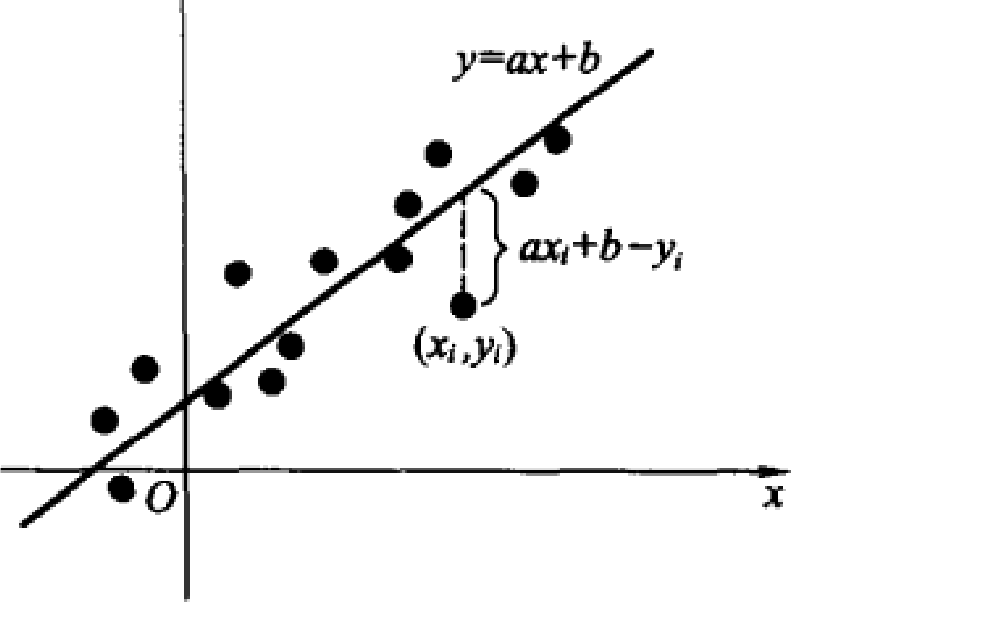
\includegraphics[width=0.42\textwidth]{work/figures/fig18-3}\caption{\relax}\label{fig:18-3}
\end{figure}

其中 $\rho_{1}$ 和 $\rho_{2}$ 由于绝对值的出现，用起来不大方便．而 $\rho_{3}$ 用乘方代替了 $\rho_{2}$ 中的绝对值，用起来就方便多了．这种使 $\rho_{3}$ 取最小即使所有点的误差的平方和取最小来确定拟合曲线的方法，就称为最小二乘法，它是由高斯（Gauss，1777—1855）首创的．在拟合曲线是直线的情形，最小二乘法就是确定 $a$，$b$，使 $\rho_{3}$ 达到最小．

记
\[
f(a,b)=\sum_{i=1}^{n}\left(ax_{i}+b-y_{i}\right)^{2}.
\]
为求其最小，分别对 $a$，$b$ 求偏导数，并令它们等于 $0$：
\[
\begin{aligned}
\frac{\partial f}{\partial a}&=2\sum_{i=1}^{n}\left(ax_{i}+b-y_{i}\right)x_{i}=0,\\
\frac{\partial f}{\partial b}&=2\sum_{i=1}^{n}\left(ax_{i}+b-y_{i}\right)=0,
\end{aligned}
\]
写出来就是
\[
\begin{cases}
\displaystyle a\sum_{i=1}^{n}x_{i}^{2}+b\sum_{i=1}^{n}x_{i}=\sum_{i=1}^{n}x_{i}y_{i},\\[3mm]
\displaystyle a\sum_{i=1}^{n}x_{i}+bn=\sum_{i=1}^{n}y_{i}.
\end{cases}
\]
为了把方程的解写清楚，记 $\bm{x}=(x_{1},x_{2},\cdots,x_{n})$，$\bm{y}=(y_{1},y_{2},\cdots,y_{n})$，$\bm{e}=(1,1,\cdots,1)$．引入内积
\[
(\bm{x},\bm{y})=\sum_{i=1}^{n}x_{i}y_{i},
\]
则上述方程组可以写为
\[
\begin{cases}
(\bm{x},\bm{x})a+(\bm{x},\bm{e})b=(\bm{x},\bm{y}),\\
(\bm{x},\bm{e})a+(\bm{e},\bm{e})b=(\bm{y},\bm{e}).
\end{cases}
\]
由克拉默法则，当 $\begin{vmatrix}(\bm{x},\bm{x})&(\bm{x},\bm{e})\\ (\bm{x},\bm{e})&(\bm{e},\bm{e})\end{vmatrix}\neq0$ 时，方程组有唯一解，这个解也是函数 $f$ 唯一的稳定点
\begin{equation}
\overline{a}=\frac{\begin{vmatrix}(\bm{x},\bm{y})&(\bm{x},\bm{e})\\ (\bm{y},\bm{e})&(\bm{e},\bm{e})\end{vmatrix}}{\begin{vmatrix}(\bm{x},\bm{x})&(\bm{x},\bm{e})\\ (\bm{x},\bm{e})&(\bm{e},\bm{e})\end{vmatrix}},\quad
\overline{b}=\frac{\begin{vmatrix}(\bm{x},\bm{x})&(\bm{x},\bm{y})\\ (\bm{x},\bm{e})&(\bm{y},\bm{e})\end{vmatrix}}{\begin{vmatrix}(\bm{x},\bm{x})&(\bm{x},\bm{e})\\ (\bm{x},\bm{e})&(\bm{e},\bm{e})\end{vmatrix}}.
\tag{5}
\end{equation}
由于函数 $f(a,b)$ 在全平面可微，且由实际问题知 $f$ 必有最小值，因此唯一的稳定点必是最小值点，即函数 $f(a,b)$ 在稳定点处取最小值．这样我们便求得拟合直线为
\[
y=\overline{a}x+\overline{b},
\]
其中，$\overline{a}$，$\overline{b}$ 由公式（5）给出．

最小二乘法也有它的不足之处．在测量中可能出现个别异常点，即与真实直线偏离较远的点，这时 $\left|y-y_{i}\right|$ 较大，平方后就更大．用平方和达到最小作标准，就可能导致拟合直线与真实直线偏离较大的情形（图~\ref{fig:18-4}）．从这个角度来说，$\rho_{2}$ 给出的总误差可以改善异常点带来的影响．对 $\rho_{2}$ 求最小来获得拟合直线的方法称为最小一乘法．

\begin{figure}[htbp]
\centering
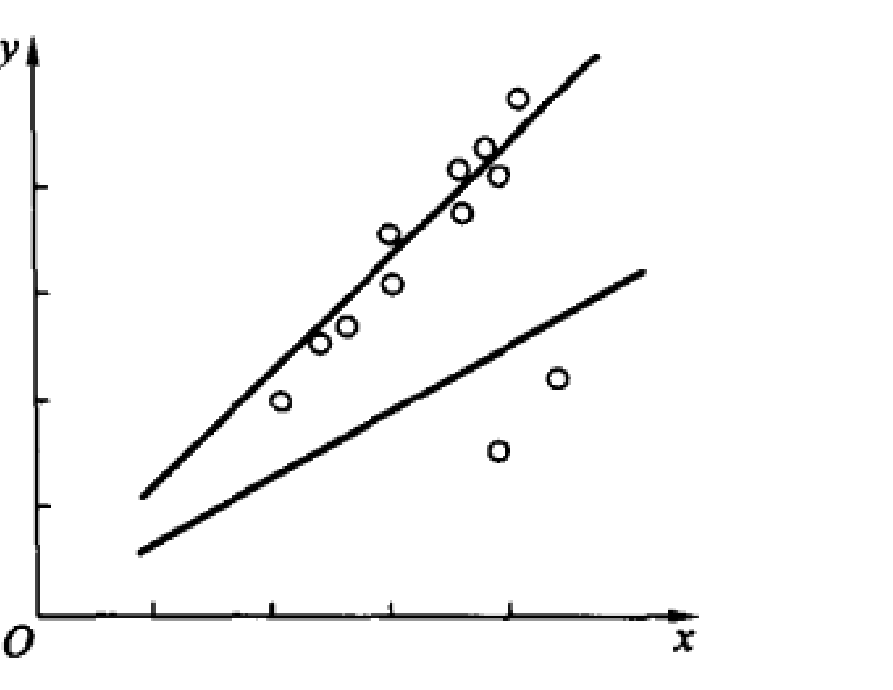
\includegraphics[width=0.4\textwidth]{work/figures/fig18-4}\caption{\relax}\label{fig:18-4}
\end{figure}

\subsection{多元函数的最值}

通过对最小二乘法的介绍，我们实际上已给出了一种利用极值求最值的方法．极值是函数 $f$ 在某点局部的性质，而最值是 $f$ 在某区域 $D$ 上的整体性质．只要搞清楚了最值与极值的关系，就可找到求最值的方法．

首先求出所有可能的最值点．函数 $f(x,y)$ 在 $D$ 上的最值点可能是 $D$ 的内点，也可能是 $D$ 的边界点．如果是 $D$ 的内点，则必是极值点．因此可能的最值点包括可能的极值点和属于 $D$ 的边界点．或者说可能的最值点就是稳定点、至少有一个偏导数不存在的点以及属于 $D$ 的边界点．

其次，我们来判别这些可能的最值点哪些是最大值点，哪些是最小值点．在已知 $f$ 于 $D$ 内存在最值的前提下，比较 $D$ 内所有可能的最值点的函数值（如果可能的话），就可确定出最大值点和最小值点．特别，若 $D$ 是开集，函数 $f$ 在 $D$ 内可导且稳定点唯一时，则唯一的稳定点就是最值点．值得指出的是，最值存在性的前提是重要的．例如马鞍面 $z=f(x,y)=xy$ 在单位圆 $D=\{(x,y)\mid x^{2}+y^{2}<1\}$ 内有唯一的稳定点 $(0,0)$，但这唯一的稳定点并不是最值点．

\begin{example}\label{ex:18-1-2}
试在 $x$ 轴，$y$ 轴与直线 $x+y=2\pi$ 围成的三角形区域上求函数 $u=\sin x+\sin y-\sin(x+y)$ 的最大值．
\end{example}

\begin{proof}[解]
所给区域为
\[
D=\left\{(x,y)\mid x+y\leqslant2\pi,x\geqslant0,y\geqslant0\right\}.
\]
函数 $u$ 在 $D$ 内可导，令
\[
\begin{cases}
\dfrac{\partial u}{\partial x}=\cos x-\cos(x+y)=0,\\[2mm]
\dfrac{\partial u}{\partial y}=\cos y-\cos(x+y)=0,
\end{cases}
\]
则有 $\cos x=\cos y$．当 $(x,y)$ 是 $D$ 的内点时必有 $x=y$，代入上式得
\[
\cos x-\cos 2x=\cos x-2\cos^{2}x+1=0,
\]
即
\[
(2\cos x+1)(1-\cos x)=0.
\]

\begin{figure}[htbp]
\centering
\begin{tikzpicture}[scale=0.8,baseline=(current bounding box.center)]
  % axes
  \draw[{-Latex}] (0,0) -- (4.3,0) node[below left] {$x$};
  \draw[{-Latex}] (0,0) -- (0,3.5) node[left] {$y$};
  \node[below left] at (0,0) {$O$};
  % shaded triangle
  \draw[pattern=north east lines] (0,0) -- (3.14,0) -- (0,3.14) -- cycle;
  % line x+y=2pi
  \draw[thick] (0,3.14) -- (3.14,0) node[midway,above,sloped] {$x+y=2\pi$};
  % tick labels
  \node[below] at (3.14,0) {$2\pi$};
  \node[left] at (0,3.14) {$2\pi$};
\end{tikzpicture}\caption{\relax}\label{fig:18-5}
\end{figure}

在 $D$ 的内部只有唯一的稳定点 $\left(\dfrac{2}{3}\pi,\dfrac{2}{3}\pi\right)$．函数 $u$ 在有界闭集 $D$ 上连续，故必存在最大值．比较边界上的函数值及稳定点的函数值：在稳定点的函数值 $u\left(\dfrac{2}{3}\pi,\dfrac{2}{3}\pi\right)=\dfrac{3}{2}\sqrt{3}$；在边界 $x=0$ 上，$u=0$；在边界 $y=0$ 上，$u=0$；在边界 $x+y=2\pi$ 上，
\[
u=\sin x+\sin y=\sin x+\sin(2\pi-x)=0.
\]
故最大值为 $\dfrac{3}{2}\sqrt{3}$，最大值点为 $\left(\dfrac{2}{3}\pi,\dfrac{2}{3}\pi\right)$．
\end{proof}

\begin{example}\label{ex:18-1-3}
证明 $t\geqslant1$，$s\geqslant0$ 时，$ts\leqslant t\ln t-t+\mathrm{e}^{s}$．
\end{example}

\begin{proof}
只要证 $f(s,t)=t\ln t-t+\mathrm{e}^{s}-ts$ 在 $D=\left\{(s,t)\mid s\geqslant0,t\geqslant1\right\}$ 上有最小值 $m\geqslant0$．令
\[
\begin{cases}
\dfrac{\partial f}{\partial s}=\mathrm{e}^{s}-t=0,\\[2mm]
\dfrac{\partial f}{\partial t}=\ln t-s=0,
\end{cases}
\]
解得 $\mathrm{e}^{s}=t$．这时有无穷多个稳定点，它们形成一条平面曲线．

下面我们用最小值的定义来说明稳定点是最小值点．固定 $t=t_{0}\geqslant1$，则有
\[
\frac{\partial f}{\partial s}<0,\ \text{当}\ 0\leqslant s<\ln t_{0}\ \text{时},
\]
\[
\frac{\partial f}{\partial s}>0,\ \text{当}\ \ln t_{0}<s\ \text{时},
\]

\begin{figure}[htbp]
\centering
\begin{tikzpicture}[scale=0.8,baseline=(current bounding box.center)]
  % axes: horizontal s, vertical t
  \draw[{-Latex}] (0,0) -- (4,0) node[below left] {$s$};
  \draw[{-Latex}] (0,0) -- (0,3.6) node[left] {$t$};
  \node[below left] at (0,0) {$O$};
  % curve t = e^s
  \draw[thick,domain=0:1.2,smooth,variable=\x] plot(\x,{exp(\x)});
  \node[right] at (1.2,{exp(1.2)}) {$t=\mathrm{e}^{s}$};
\end{tikzpicture}\caption{\relax}\label{fig:18-6}
\end{figure}

故在半直线 $t=t_{0}$ $(s\geqslant0)$ 上，$f$ 在 $(\ln t_{0},t_{0})$ 达到最小值．可见 $f$ 在 $D$ 上的最小值只能在曲线 $\mathrm{e}^{s}=t$ 上达到．但
\[
f(s,\mathrm{e}^{s})=\mathrm{e}^{s}s-\mathrm{e}^{s}+\mathrm{e}^{s}-\mathrm{e}^{s}s=0.
\]
从而有
\[
f(s,t)\geqslant0,\quad(s,t)\in D.
\]
\end{proof}

\begin{xiti}
\item 求下列函数的极大值点和极小值点：
\begin{ziti}
\item $f(x,y)=(x-y+1)^{2}$；
\item $f(x,y)=3axy-x^{3}-y^{3}$ $(a>0)$；
\item $f(x,y)=xy\sqrt{1-\dfrac{x^{2}}{a^{2}}-\dfrac{y^{2}}{b^{2}}}$ $(a,b>0)$；
\item $f(x,y)=\mathrm{e}^{2x}(x+y^{2}+2y)$；
\item $f(x,y)=\sin x+\cos y+\cos(x-y)$ $\left(0\leqslant x,y\leqslant\dfrac{\pi}{2}\right)$；
\item $f(x,y)=\left(\sqrt{x^{2}+y^{2}}-1\right)^{2}$．
\end{ziti}
\item 已知 $y=ax^{2}+bx+c$，观测得一组数据 $(x_{i},y_{i})$，$i=1,2,\cdots,n$，利用最小二乘法，求系数 $a$，$b$，$c$ 所满足的三元一次方程组．
\item 已知平面上 $n$ 个点的坐标分别是
\[
A_{1}(x_{1},y_{1}),A_{2}(x_{2},y_{2}),\cdots,A_{n}(x_{n},y_{n}),
\]
试求一点，使它与这 $n$ 个点距离的平方和最小．
\item 求下列函数在指定范围 $D$ 内的最大值和最小值：
\begin{ziti}
\item $f(x,y)=x^{2}-y^{2}$，$D=\left\{(x,y)\mid x^{2}+y^{2}\leqslant4\right\}$；
\item $f(x,y)=x^{2}-xy+y^{2}$，$D=\left\{(x,y)\mid\left|x\right|+\left|y\right|\leqslant1\right\}$；
\item $f(x,y,z)=(ax+by+cz)\mathrm{e}^{-(x^{2}+y^{2}+z^{2})}$，其中 $a^{2}+b^{2}+c^{2}>0$，$D=\mathbf{R}^{3}$．
\end{ziti}
\item 求证：
\begin{ziti}
\item $f(x,y)=Ax^{2}+2Bxy+Cy^{2}+2Dx+2Ey+F$ 在 $\mathbf{R}^{2}$ 有最小值，无最大值，其中 $A>0$，$B^{2}<AC$；
\item $f(x,y)=xy+\dfrac{1}{x}+\dfrac{1}{y}$ 在 $0<x$，$y<+\infty$ 有最小值，无最大值．
\end{ziti}
\item 设 $F(x,y,z)$ 有二阶连续偏导数，并且
\[
F(x_{0},y_{0},z_{0})=0,\quad F_{z}(x_{0},y_{0},z_{0})\neq0.
\]
讨论由 $F(x,y,z)=0$ 确定的隐函数 $z=f(x,y)$ 在 $(x_{0},y_{0})$ 取得极值的必要和充分条件．再求由
\[
x^{2}+y^{2}+z^{2}-2x+2y-4z-10=0
\]
所确定的 $z=f(x,y)$ 的极值．
\item 求下列隐函数的极大值和极小值：
\begin{ziti}
\item $(x+y)^{2}+(y+z)^{2}+(z+x)^{2}=3$；
\item $z^{2}+xyz-x^{2}-xy^{2}-9=0$．
\end{ziti}
\item 在已知周长为 $2p$ 的一切三角形中，求出面积为最大的三角形．
\item 有一块铁片，宽 $b=24\ \mathrm{cm}$，要把它的两边折起做成一个槽，使得容积最大，求每边的倾角 $\alpha$ 和折起的宽度 $x$（见下图）．

\begin{center}
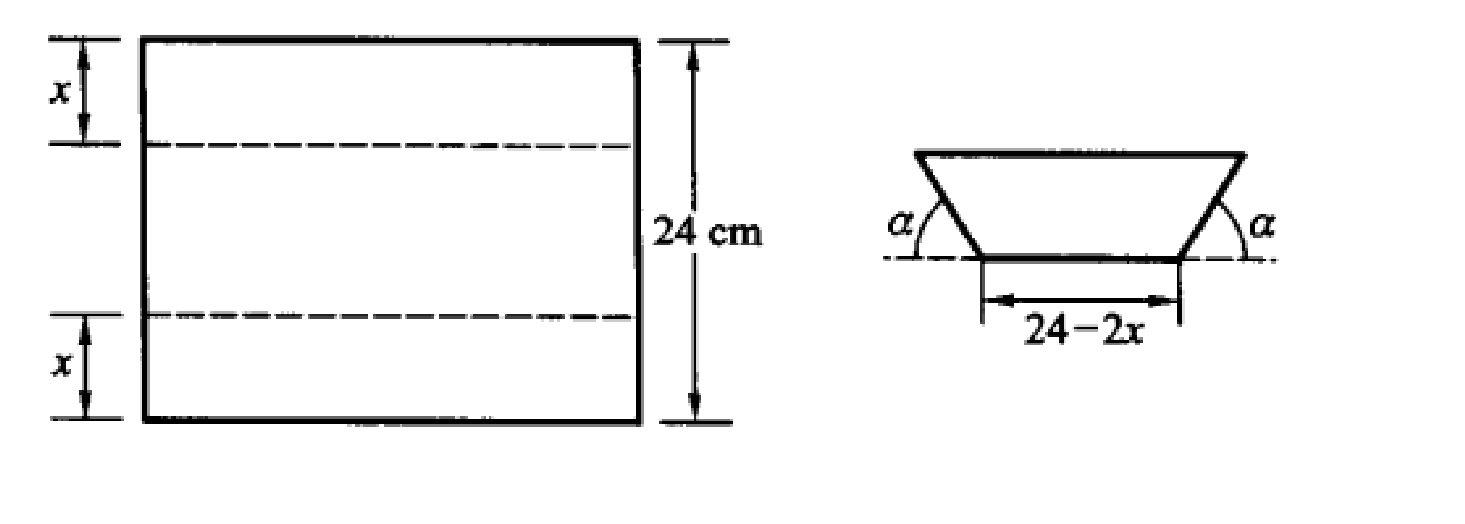
\includegraphics[width=0.66\textwidth]{work/figures/fig18-ex9}
\end{center}
\end{xiti}

\section{条件极值与拉格朗日乘数法}

前面我们考虑了函数 $f$ 在某区域 $D$ 上的极值问题．但实际问题中，函数 $f$ 的自变量不仅限制在某个区域上，它还可能受到其他条件的约束．例如，求单位球内截长方体，使其体积最大．如果取单位球面的方程 $x^{2}+y^{2}+z^{2}=1$，这时长方体的长、宽、高分别为 $2x$，$2y$，$2z$，因此长方体的体积为 $V=8xyz$．故抽象出来的数学问题是求目标函数
\[
V=8xyz
\]
满足约束条件
\[
\begin{cases}
x^{2}+y^{2}+z^{2}=1,\\
x,\quad y,\quad z>0
\end{cases}
\]
的最大值．这时函数 $V$ 的自变量 $x$，$y$，$z$ 不仅要满足定义域 $x$，$y$，$z>0$ 的要求，而且要满足条件 $x^{2}+y^{2}+z^{2}=1$．这类带有约束条件的极值问题就称为\emph{条件极值}问题．而前面讨论的不带约束条件的极值问题就称为无条件极值或普通极值问题．

条件极值有时可以化为无条件极值来求解．比如上面的条件极值问题，从球面方程中可解出 $z=\sqrt{1-x^{2}-y^{2}}$，代入目标函数，则问题等价于求
\[
V=8xy\sqrt{1-x^{2}-y^{2}}
\]
在区域 $D=\left\{(x,y)\mid x^{2}+y^{2}\leqslant1,x\geqslant0,y\geqslant0\right\}$ 的无条件极值．

条件极值问题的一般形式为求目标函数
\[
y=f(x_{1},x_{2},\cdots,x_{n})
\]
在约束条件
\[
g_{k}(x_{1},x_{2},\cdots,x_{n})=0,\quad k=1,2,\cdots,m\ (m<n)
\]
下的极值．

也就是说，约束方程可以有多个，而且它们可能对各变量来说都是隐式．这时要从约束条件方程组中解出 $m$ 个显函数是非常困难甚至是不可能的．因此，希望寻求一种无需解出显函数来的方法．我们讨论 $n=4$，$m=2$ 这种较简单的情形，但方法已具有一般性．这时是要求目标函数 $f(x,y,u,v)$ 在约束条件
\begin{equation}
\begin{cases}
F(x,y,u,v)=0,\\
G(x,y,u,v)=0
\end{cases}
\tag{1}
\end{equation}
下的条件极值，其中 $(x,y,u,v)\in U$．

以极小值为例，称点 $P_{0}(x_{0},y_{0},u_{0},v_{0})$ 是函数 $f$ 在条件（1）下的极小值点，如果 $P_{0}$ 满足（1）式，且存在 $P_{0}$ 点的某邻域 $O(P_{0})\subset U$，使得对任意满足（1）式的 $P(x,y,u,v)\in O(P_{0})$，有
\begin{equation}
f(x,y,u,v)\geqslant f(x_{0},y_{0},u_{0},v_{0}).
\tag{2}
\end{equation}
为了能用微分学来进行研究，假设 $f$，$F$，$G$ 在 $U$ 内具有对各变元的连续偏导数．我们主要考虑取极值的必要条件．

设点 $P_{0}(x_{0},y_{0},u_{0},v_{0})$ 是函数 $f$ 在条件（1）下的极值点，则
\begin{equation}
F(P_{0})=G(P_{0})=0,
\tag{3}
\end{equation}
且（2）式成立．如果 $\left.\dfrac{\partial(F,G)}{\partial(u,v)}\right|_{P_{0}}\neq0$，那么由隐函数组存在定理知，在 $P_{0}$ 点的某邻域内，方程组（1）唯一地确定一组可微函数
\[
\begin{cases}
u=u(x,y),\\
v=v(x,y),
\end{cases}
\]
它定义在 $(x_{0},y_{0})$ 的某邻域 $D$ 内，当 $(x,y)\in D$ 时，$(x,y,u,v)\in U$，且这组函数满足方程组（1）和
\[
u_{0}=u(x_{0},y_{0}),\ v_{0}=(x_{0},y_{0}).
\]
这时（2）式等价于说，$(x_{0},y_{0})$ 是函数
\[
g(x,y)=f(x,y,u(x,y),v(x,y))
\]
的无条件极值点．由无条件极值的必要条件知，$(x_{0},y_{0})$ 必须满足
\begin{equation}
\mathrm{d}g(x_{0},y_{0})=\left\{\frac{\partial f}{\partial x}\mathrm{d}x+\frac{\partial f}{\partial y}\mathrm{d}y+\frac{\partial f}{\partial u}\mathrm{d}u+\frac{\partial f}{\partial v}\mathrm{d}v\right\}_{(x_{0},y_{0})}=0.
\tag{4}
\end{equation}
注意这里 $\mathrm{d}x$，$\mathrm{d}y$，$\mathrm{d}u$，$\mathrm{d}v$ 不是独立的，它们在 $P_{0}(x_{0},y_{0},u_{0},v_{0})$ 满足
\begin{align}
\mathrm{d}F(P_{0})&=\left\{\frac{\partial F}{\partial x}\mathrm{d}x+\frac{\partial F}{\partial y}\mathrm{d}y+\frac{\partial F}{\partial u}\mathrm{d}u+\frac{\partial F}{\partial v}\mathrm{d}v\right\}_{P_{0}}=0,
\tag{5}\\
\mathrm{d}G(P_{0})&=\left\{\frac{\partial G}{\partial x}\mathrm{d}x+\frac{\partial G}{\partial y}\mathrm{d}y+\frac{\partial G}{\partial u}\mathrm{d}u+\frac{\partial G}{\partial v}\mathrm{d}v\right\}_{P_{0}}=0.
\tag{6}
\end{align}
将（5）式（6）式分别乘以 $\lambda_{1}$ 和 $\lambda_{2}$ 后与（4）式一起相加得
\begin{equation}
\begin{aligned}
\bigg\{\left(\frac{\partial f}{\partial x}+\lambda_{1}\frac{\partial F}{\partial x}+\lambda_{2}\frac{\partial G}{\partial x}\right)&\mathrm{d}x+\left(\frac{\partial f}{\partial y}+\lambda_{1}\frac{\partial F}{\partial y}+\lambda_{2}\frac{\partial G}{\partial y}\right)\mathrm{d}y+\\
\left(\frac{\partial f}{\partial u}+\lambda_{1}\frac{\partial F}{\partial u}+\lambda_{2}\frac{\partial G}{\partial u}\right)&\mathrm{d}u+\left(\frac{\partial f}{\partial v}+\lambda_{1}\frac{\partial F}{\partial v}+\lambda_{2}\frac{\partial G}{\partial v}\right)\mathrm{d}v\bigg\}_{P_{0}}=0,
\end{aligned}
\tag{7}
\end{equation}
其中 $\lambda_{1}$，$\lambda_{2}$ 待定．由于 $\mathrm{d}x$，$\mathrm{d}y$，$\mathrm{d}u$，$\mathrm{d}v$ 不独立，故不能从（7）推出 $\mathrm{d}x$，$\mathrm{d}y$，$\mathrm{d}u$，$\mathrm{d}v$ 的系数等于零．但已知 $\left.\dfrac{\partial(F,G)}{\partial(u,v)}\right|_{P_{0}}\neq0$，故方程组
\[
\begin{cases}
\dfrac{\partial f}{\partial u}+\lambda_{1}\dfrac{\partial F}{\partial u}+\lambda_{2}\dfrac{\partial G}{\partial u}=0,\\[2mm]
\dfrac{\partial f}{\partial v}+\lambda_{1}\dfrac{\partial F}{\partial v}+\lambda_{2}\dfrac{\partial G}{\partial v}=0
\end{cases}
\]
在 $P_{0}$ 点有唯一解 $(\lambda_{1},\lambda_{2})$，这时（7）式化为
\[
\left\{\left(\frac{\partial f}{\partial x}+\lambda_{1}\frac{\partial F}{\partial x}+\lambda_{2}\frac{\partial G}{\partial x}\right)\mathrm{d}x+\left(\frac{\partial f}{\partial y}+\lambda_{1}\frac{\partial F}{\partial y}+\lambda_{2}\frac{\partial G}{\partial y}\right)\mathrm{d}y\right\}_{P_{0}}=0.
\]
由于 $\mathrm{d}x$，$\mathrm{d}y$ 独立，则它们的系数等于零，于是得 $P_{0}$ 及 $(\lambda_{1},\lambda_{2})$ 所满足的方程组
\[
\begin{aligned}
\frac{\partial f}{\partial x}+\lambda_{1}\frac{\partial F}{\partial x}+\lambda_{2}\frac{\partial G}{\partial x}&=0,\\
\frac{\partial f}{\partial y}+\lambda_{1}\frac{\partial F}{\partial y}+\lambda_{2}\frac{\partial G}{\partial y}&=0,\\
\frac{\partial f}{\partial u}+\lambda_{1}\frac{\partial F}{\partial u}+\lambda_{2}\frac{\partial G}{\partial u}&=0,\\
\frac{\partial f}{\partial v}+\lambda_{1}\frac{\partial F}{\partial v}+\lambda_{2}\frac{\partial G}{\partial v}&=0,\\
F(x,y,u,v)&=0,\\
G(x,y,u,v)&=0.
\end{aligned}
\]
方程组含 $6$ 个方程，$6$ 个未知数 $(x,y,u,v,\lambda_{1},\lambda_{2})$，一般说来是可以由此解出 $(x_{0},y_{0},u_{0},v_{0})$ 和 $(\lambda_{1},\lambda_{2})$ 的．这时 $(x_{0},y_{0},u_{0},v_{0})$ 就是 $f(x,y,u,v)$ 在条件（1）下的稳定点，而 $(x_{0},y_{0})$ 就是函数 $g(x,y)$ 的无条件极值的稳定点．

引入辅助函数
\begin{equation}
L(x,y,u,v)=f(x,y,u,v)+\lambda_{1}F(x,y,u,v)+\lambda_{2}G(x,y,u,v),
\tag{8}
\end{equation}
则上述方程组前四个式子恰为
\[
L_{x}(P_{0})=L_{y}(P_{0})=L_{u}(P_{0})=L_{v}(P_{0})=0.
\]
（8）式定义的函数称为拉格朗日函数，而 $\lambda_{1}$，$\lambda_{2}$ 称为拉格朗日乘数．上面的讨论即是说：若 $P_{0}(x_{0},y_{0},u_{0},v_{0})$ 是函数 $f$ 在条件（1）下的条件极值点，则 $P_{0}$ 是拉格朗日函数的稳定点，且 $P_{0}$ 满足约束条件（1）．我们把上面的推理总结为下面的定理．

\begin{theorem}\label{thm:18-3}
若 $f(x,y,u,v)$，$F(x,y,u,v)$，$G(x,y,u,v)$ 在点 $P_{0}(x_{0},y_{0},$ $u_{0},v_{0})$ 的某邻域有连续的偏导数，且函数 $f$ 在约束条件（1）下在 $P_{0}$ 点取极值，矩阵
\begin{equation}
\left.\begin{pmatrix}F_{x}&F_{y}&F_{u}&F_{v}\\ G_{x}&G_{y}&G_{u}&G_{v}\end{pmatrix}\right|_{P_{0}}
\tag{9}
\end{equation}
的秩为 $2$，则存在唯一确定的 $\lambda_{1},\lambda_{2}$，使得
\begin{equation}
\begin{cases}
L_{x}(P_{0})=L_{y}(P_{0})=L_{u}(P_{0})=L_{v}(P_{0})=0,\\
F(P_{0})=G(P_{0})=0,
\end{cases}
\tag{10}
\end{equation}
其中 $L(x,y,u,v)$ 是拉格朗日函数，其定义为 $L=f+\lambda_{1}F+\lambda_{2}G$．
\end{theorem}

注意（10）式中有六个方程，由它可以确定六个未知数 $(x_{0},y_{0},u_{0},v_{0})$ 和 $\lambda_{1}$，$\lambda_{2}$．其中 $(x_{0},y_{0},u_{0},v_{0})$ 是拉格朗日函数的稳定点，从而是函数 $f(x,y,u,v)$ 的可能条件极值点，而 $(x_{0},y_{0})$ 就是函数 $g(x,y)$ 的可能无条件极值点．又因为 $(x_{0},y_{0},u_{0},v_{0})$ 是 $f(x,y,u,v)$ 的条件极值点等价于 $(x_{0},y_{0})$ 是 $g(x,y)$ 的无条件极值点，故只要用无条件极值的充分条件即可判别稳定点 $(x_{0},y_{0},u_{0},v_{0})$ 是否为 $f$ 的条件极值点．

值得指出的是，我们用矩阵（9）的秩为 $2$ 代替了条件 $\left.\dfrac{\partial(F,G)}{\partial(u,v)}\right|_{P_{0}}\neq0$，其理由是，由（9）的秩为 $2$ 知总有一个二阶行列式不为零，对此进行类似于上述的推理，便得到一样的结果．读者应注意到所有变量 $x$，$y$，$u$，$v$ 在方程组（10）中的位置是对等的．

现在我们回头来解本节开头提出的问题：求 $V=8xyz$ 满足约束条件
\[
x^{2}+y^{2}+z^{2}=1,\ x,y,z>0
\]
的最大值．

作拉格朗日函数
\[
L(x,y,z)=8xyz+\lambda(x^{2}+y^{2}+z^{2}-1).
\]
令
\[
\begin{aligned}
L_{x}&=8yz+2\lambda x=0,\\
L_{y}&=8xz+2\lambda y=0,\\
L_{z}&=8xy+2\lambda z=0,\\
x^{2}+y^{2}+z^{2}&=1.
\end{aligned}
\]
由前三式及 $x>0$，$y>0$，$z>0$ 得
\[
8xyz=-2\lambda x^{2}=-2\lambda y^{2}=-2\lambda z^{2},
\]
从而 $x=y=z$，代入最后一式得
\[
3x^{2}=1,
\]
解得拉格朗日函数的稳定点为
\[
x=y=z=\frac{1}{\sqrt{3}}.
\]
由实际问题知所求最大值必存在，而稳定点又唯一，因此唯一的稳定点就是最大值点．故球内截长方体中以正方体的体积为最大．

\begin{example}\label{ex:18-2-1}
求 $f(x,y,z)=xyz$ 在条件 $\dfrac{1}{x}+\dfrac{1}{y}+\dfrac{1}{z}=\dfrac{1}{r}$ $(x>0,y>0,z>0,r>0)$ 下的极小值；并证明不等式
\[
3\left(\frac{1}{x}+\frac{1}{y}+\frac{1}{z}\right)^{-1}\leqslant\sqrt[3]{xyz},
\]
其中 $x$，$y$，$z$ 为任意正实数．
\end{example}

\begin{proof}[解]
作拉格朗日函数
\[
L(x,y,z)=xyz+\lambda\left(\frac{1}{x}+\frac{1}{y}+\frac{1}{z}-\frac{1}{r}\right).
\]
令
\[
\begin{cases}
L_{x}=yz-\dfrac{\lambda}{x^{2}}=0,\\[2mm]
L_{y}=xz-\dfrac{\lambda}{y^{2}}=0,\\[2mm]
L_{z}=xy-\dfrac{\lambda}{z^{2}}=0,\\[2mm]
\dfrac{1}{x}+\dfrac{1}{y}+\dfrac{1}{z}=\dfrac{1}{r}.
\end{cases}
\]
由前三式得
\[
xyz=\frac{\lambda}{x}=\frac{\lambda}{y}=\frac{\lambda}{z}.
\]
因此，$x=y=z$．把它代入最后一式即得拉格朗日函数的稳定点为
\[
x=y=z=3r.
\]
下面判别稳定点是极值点．若记 $F(x,y,z)=\dfrac{1}{x}+\dfrac{1}{y}+\dfrac{1}{z}-\dfrac{1}{r}$，则 $F_{z}(3r,$ $3r,3r)=-\left.\dfrac{1}{z^{2}}\right|_{z=3r}\neq0$．故方程
\[
\frac{1}{x}+\frac{1}{y}+\frac{1}{z}=\frac{1}{r}
\]
在稳定点的附近可唯一地确定可微函数 $z=z(x,y)$．令
\[
g(x,y)=f(x,y,z(x,y)),
\]
我们用二元函数取无条件极值的充分条件判别 $(3r,3r)$ 是 $g(x,y)$ 的极值点．由约束条件得
\[
\frac{\partial z}{\partial x}=-\frac{z^{2}}{x^{2}},\quad\frac{\partial z}{\partial y}=-\frac{z^{2}}{y^{2}}.
\]
由复合函数链式法则
\[
\begin{aligned}
\frac{\partial g}{\partial x}&=yz+xy\frac{\partial z}{\partial x}=yz-\frac{yz^{2}}{x},\\
\frac{\partial g}{\partial y}&=xz+xy\frac{\partial z}{\partial y}=xz-\frac{xz^{2}}{y},\\
\frac{\partial^{2}g}{\partial x^{2}}&=y\frac{\partial z}{\partial x}+\frac{yz^{2}}{x^{2}}-\frac{2yz}{x}\frac{\partial z}{\partial x}=\frac{2yz^{3}}{x^{3}},\\
\frac{\partial^{2}g}{\partial x\partial y}&=z+y\frac{\partial z}{\partial y}-\frac{z^{2}}{x}-\frac{2yz}{x}\frac{\partial z}{\partial y}=z-\frac{z^{2}}{y}-\frac{z^{2}}{x}+\frac{2z^{3}}{xy},\\
\frac{\partial^{2}g}{\partial y^{2}}&=\frac{2xz^{3}}{y^{3}}.
\end{aligned}
\]
故函数 $g$ 在 $(3r,3r)$ 点有
\[
\left|\begin{array}{cc}a_{11}&a_{12}\\ a_{12}&a_{22}\end{array}\right|=\left|\begin{array}{cc}6r&3r\\ 3r&6r\end{array}\right|=36r^{2}-9r^{2}=27r^{2}>0,
\]
且 $a_{11}=6r>0$．因此 $g(x,y)$ 在 $(3r,3r)$ 处取极小值，这等价于 $f(x,y,z)$ 在 $(3r,3r,3r)$ 处取条件极小值
\[
f(3r,3r,3r)=(3r)^{3}.
\]
分析约束集 $D$：
\[
D=\left\{(x,y,z)\mid\frac{1}{x}+\frac{1}{y}+\frac{1}{z}=\frac{1}{r},\ x>0,y>0,z>0\right\},
\]
它是一无界集，当 $(x,y,z)$ 在 $D$ 内远离坐标原点时，函数 $f$ 将趋于正无穷．因此，函数 $f$ 的唯一极小值点是函数的最小值点，即有
\[
xyz\geqslant(3r)^{3},\quad(x,y,z)\in D.
\]
由于在 $D$ 内有 $r=\left(\dfrac{1}{x}+\dfrac{1}{y}+\dfrac{1}{z}\right)^{-1}$，代入上式即得
\[
3\left(\frac{1}{x}+\frac{1}{y}+\frac{1}{z}\right)^{-1}\leqslant\sqrt[3]{xyz},\ x,y,z>0.
\]
注意上式又可写为
\[
\sqrt[3]{\frac{1}{xyz}}\leqslant\frac{\dfrac{1}{x}+\dfrac{1}{y}+\dfrac{1}{z}}{3},
\]
这就是我们熟悉的平均值不等式：三个正实数 $\dfrac{1}{x}$，$\dfrac{1}{y}$，$\dfrac{1}{z}$ 的几何平均与算术平均的关系．
\end{proof}

\begin{example}\label{ex:18-2-2}
求函数 $f=x+y+z+t$ 在约束条件 $xyzt=c^{4}$（其中 $x,y,z,t,c>0$）下的极值．
\end{example}

\begin{proof}[解]
作拉格朗日函数
\[
L(x,y,z,t)=x+y+z+t+\lambda(xyzt-c^{4}).
\]
令
\[
\begin{cases}
L_{x}=1+\lambda yzt=0,\\
L_{y}=1+\lambda xzt=0,\\
L_{z}=1+\lambda xyt=0,\\
L_{t}=1+\lambda xyz=0,\\
xyzt=c^{4}.
\end{cases}
\]
由前四式得
\[
-\lambda xyzt=x=y=z=t\ \text{；}
\]
再从最后一式解得稳定点
\[
x=y=z=t=c.
\]
下面判定稳定点是极值点．注意此例中函数 $f$ 有 $4$ 个自变量，但只有一个约束条件．由约束条件确定出某个隐函数代入 $f$ 后，则 $f$ 还有 $3$ 个独立的自变量，因此不能类似上例用定理 18.2 来判别．为此我们用 $\mathrm{d}^{2}f(c,c,c,c)$ 的符号来判别是否极值．

在求微分之前，我们必须搞清楚变量之间的关系．由于有一个约束条件 $xyzt=c^{4}$，变量 $x$，$y$，$z$，$t$ 之间不是独立的，从而 $\mathrm{d}x$，$\mathrm{d}y$，$\mathrm{d}z$，$\mathrm{d}t$ 之间也不是独立的．它们之间的关系可以通过在约束条件等式两边求微分而得到：
\begin{equation}
yzt\mathrm{d}x+xzt\mathrm{d}y+xyt\mathrm{d}z+xyz\mathrm{d}t=0.
\tag{11}
\end{equation}
特别在稳定点 $(c,c,c,c)$ 处 $\mathrm{d}x,\mathrm{d}y,\mathrm{d}z,\mathrm{d}t$ 应满足
\begin{equation}
\mathrm{d}x+\mathrm{d}y+\mathrm{d}z+\mathrm{d}t=0.
\tag{12}
\end{equation}
也就是说，四个变量中只有三个是独立变量．这里不妨取 $x$，$y$，$z$ 为独立变量，则 $t$ 是 $x$，$y$，$z$ 的函数，那么（11）（12）式中 $\mathrm{d}x$，$\mathrm{d}y$，$\mathrm{d}z$ 是自变量的微分，而 $\mathrm{d}t$ 是函数的微分．这时 $f=f(x,y,z,t(x,y,z))$．

明确了上述变量之间的关系后，我们来求微分．由一阶微分形式不变性有
\[
\mathrm{d}f=\mathrm{d}x+\mathrm{d}y+\mathrm{d}z+\mathrm{d}t,
\]
其中 $\mathrm{d}x,\mathrm{d}y,\mathrm{d}z,\mathrm{d}t$ 满足（11）式，从而
\[
\mathrm{d}^{2}f=\mathrm{d}^{2}t.
\]
为求 $\mathrm{d}^{2}t$，在（11）式两边再求微分，得
\[
\begin{aligned}
&\left(zt\mathrm{d}y+yt\mathrm{d}z+yz\mathrm{d}t\right)\mathrm{d}x+\left(zt\mathrm{d}x+xt\mathrm{d}z+xz\mathrm{d}t\right)\mathrm{d}y+\\
&\left(yt\mathrm{d}x+xt\mathrm{d}y+xy\mathrm{d}t\right)\mathrm{d}z+\left(yz\mathrm{d}x+xz\mathrm{d}y+xy\mathrm{d}z\right)\mathrm{d}t+\\
&xyz\mathrm{d}^{2}t=0,
\end{aligned}
\]
在上式中令 $x=y=z=t=c$，得
\[
\mathrm{d}^{2}t=\frac{-2}{c}\left[\mathrm{d}x\mathrm{d}y+\mathrm{d}y\mathrm{d}z+\mathrm{d}x\mathrm{d}z+\mathrm{d}t\left(\mathrm{d}x+\mathrm{d}y+\mathrm{d}z\right)\right],
\]
其中 $\mathrm{d}x,\mathrm{d}y,\mathrm{d}z,\mathrm{d}t$ 满足（12）式，将（12）式代入得
\[
\begin{aligned}
\mathrm{d}^{2}t&=-\frac{2}{c}\left[\mathrm{d}x\mathrm{d}y+\mathrm{d}y\mathrm{d}z+\mathrm{d}x\mathrm{d}z-\left(\mathrm{d}x+\mathrm{d}y+\mathrm{d}z\right)^{2}\right]\\
&=\frac{1}{c}\left[\left(\mathrm{d}x+\mathrm{d}y+\mathrm{d}z\right)^{2}+\mathrm{d}x^{2}+\mathrm{d}y^{2}+\mathrm{d}z^{2}\right]>0,
\end{aligned}
\]
即
\[
\left.\mathrm{d}^{2}f\right|_{(c,c,c,c)}>0.
\]
因此函数 $f$ 在 $(c,c,c,c)$ 取条件极小值，$f(c,c,c,c)=4c$．
\end{proof}

前面我们已经看到，利用拉格朗日函数 $L(P)$，使我们可以方便地求得可能的条件极值点．其实，利用拉格朗日函数 $L(P)$ 还可以判别可能的极值点是否确是极值点，即有下述结论：

设 $P_{0}$ 是拉格朗日函数的稳定点，则

（1）若 $\mathrm{d}^{2}L(P_{0})>0$，则 $f$ 在 $P_{0}$ 取条件极小；

（2）若 $\mathrm{d}^{2}L(P_{0})<0$，则 $f$ 在 $P_{0}$ 取条件极大．我们把证明留给读者（习题 11）．

这个结论和必要条件（定理 18.3）一起表明，拉格朗日函数使条件极值问题完全化为了无条件极值．它消除了约束条件的影响，使所有变量处于平等地位．这个方法是拉格朗日引进的，称为拉格朗日乘数法，它简明优美，可算应用数学的一个典范．

\begin{xiti}
\item 求下列函数在所给条件下的极值：
\begin{ziti}
\item $f=x+y$，若 $x^{2}+y^{2}=1$；
\item $f=x^{2}+y^{2}$，若 $x+y-1=0$；
\item $f=x-2y+2z$，若 $x^{2}+y^{2}+z^{2}=1$；
\item $f=\dfrac{1}{x}+\dfrac{1}{y}$，若 $x+y=2$；
\item $f=xyz$，若 $x^{2}+y^{2}+z^{2}=1$，$x+y+z=0$；
\item $f=ax^{2}+by^{2}+2hxy$，若 $x^{2}+y^{2}=1$；
\item $f=x^{2}+y^{2}+z^{2}$，若 $(x^{2}+y^{2}+z^{2})^{2}=a^{2}x^{2}+b^{2}y^{2}+c^{2}z^{2}$，$lx+my+nz=0$．
\end{ziti}
\item 求 $f=x^{m}y^{n}z^{p}$ 在条件 $x+y+z=a$，$a>0$，$m>0$，$n>0$，$p>0$，$x>0$，$y>0$，$z>0$ 之下的最大值．
\item 求函数 $z=\dfrac{1}{2}(x^{n}+y^{n})$ 在条件 $x+y=l$ $(l>0,n\geqslant1)$ 之下的极值，并证明：当 $a\geqslant0$，$b\geqslant0$，$n\geqslant1$ 时
\[
\left(\frac{a+b}{2}\right)^{n}\leqslant\frac{a^{n}+b^{n}}{2}.
\]
\item 求表面积一定而体积最大的长方体．
\item 求体积一定而表面积最小的长方体．
\item 求圆的外切三角形中面积最小者．
\item 长为 $a$ 的铁丝切成两段，一段围成正方形，另一段围成圆．这两段的长各为多少时，它们所围正方形面积和圆面积之和最小．
\item 求原点到二平面 $a_{1}x+b_{1}y+c_{1}z+d_{1}=0$，$a_{2}x+b_{2}y+c_{2}z+d_{2}=0$ 的交线的最短距离．
\item 求抛物线 $y=x^{2}$ 和直线 $x-y=1$ 间的最短距离．
\item 求 $x>0$，$y>0$，$z>0$ 时函数 $f(x,y,z)=\ln x+2\ln y+3\ln z$ 在球面 $x^{2}+y^{2}+z^{2}=6r^{2}$ 上的极大值．证明 $a$，$b$，$c$ 为正实数时，
\[
ab^{2}c^{3}\leqslant108\left(\frac{a+b+c}{6}\right)^{6}.
\]
\item 设函数 $f(x,y,u,v)$，$F(x,y,u,v)$，$G(x,y,u,v)$ 二阶可微，雅可比矩阵
\[
\begin{pmatrix}F_{x}&F_{y}&F_{u}&F_{v}\\ G_{x}&G_{y}&G_{u}&G_{v}\end{pmatrix}
\]
的秩为 $2$．令
\[
L(x,y,u,v)=f(x,y,u,v)+\lambda_{1}F(x,y,u,v)+\lambda_{2}G(x,y,u,v),
\]
若 $P_{0}(x_{0},y_{0},u_{0},v_{0})$ 是函数 $L$ 的稳定点，证明：当 $\mathrm{d}^{2}L(P_{0})>(<)0$ 时，$P_{0}$ 是函数 $f$ 在约束条件
\[
F(x,y,u,v)=0,\quad G(x,y,u,v)=0
\]
下的条件极小（大）值点．
\end{xiti}

% !TeX program = xelatex
% 第十九章 含参变量的积分
\chapter{含参变量的积分}

为了表示函数，特别是非初等函数，我们曾经系统研究过函数项级数．函数项级数是指
\[
\sum_{n=1}^{\infty}u_{n}(x).
\]
我们已经知道，对每个 $n$，$u_{n}(x)$ 可能是很简单的函数，例如 $a_{n}x^{n}$ 或 $a_{n}\cos nx+b_{n}\sin nx$，但无穷项加起来后，却可以表示极其复杂的函数．本章研究的含参变量积分，与函数项级数十分类似，其区别之处是，级数是对离散量 $n$ 求和，而我们这里是对连续量求积分．当这种积分是有穷区间上的正常积分时，由于已有了多元函数与微积分的理论，研究起来是比较简单的．这是本章 §1 要讲述的内容．当这种积分是无穷区间或有穷区间的广义积分时，情况就同函数项级数更为类似．这时一致收敛的概念成了理论的关键，这是本章 §2 要讲述的内容．应用函数项级数的方法是 §2 的主线，掌握连续变量与离散变量的异同，则是读者学习本节要特别注意的地方．§3 将通过含参变量积分给出两个十分重要的非初等函数——贝塔（Beta）函数和伽玛（Gamma）函数．

\section{含参变量的正常积分}

设函数 $f(x,y)$ 在矩形区域 $[a,b]\times[c,d]$ 上有定义，对 $[a,b]$ 上任一固定的 $x_{0}$，$f(x_{0},y)$ 在 $[c,d]$ 上可积，则
\[
\int_{c}^{d}f(x_{0},y)\dd y
\]
就确定一个数．当 $x$ 在 $[a,b]$ 上变动时，这样的积分就定义了一个函数
\[
I(x)=\int_{c}^{d}f(x,y)\dd y,\quad x\in[a,b],
\]
称此积分为含参变量的积分，参变量为 $x$．

\begin{theorem}[积分号下取极限]\label{thm:19-1}
设 $f(x,y)$ 在矩形区域 $[a,b]\times[c,d]$ 上连续，则
\[
I(x)=\int_{c}^{d}f(x,y)\dd y
\]
在 $[a,b]$ 连续．
\end{theorem}

\begin{proof}
对任意 $x\in[a,b]$，$x+\Delta x\in[a,b]$，有
\[
I(x+\Delta x)-I(x)=\int_{c}^{d}\left[f(x+\Delta x,y)-f(x,y)\right]\dd y.
\]
由于 $f(x,y)$ 在 $[a,b]\times[c,d]$ 连续，因而一致连续，故对任给的 $\varepsilon>0$，存在 $\delta>0$，对任意的 $(x_{1},y_{1})$，$(x_{2},y_{2})\in[a,b]\times[c,d]$，只要 $|x_{1}-x_{2}|<\delta$，$|y_{1}-y_{2}|<\delta$，就有
\[
|f(x_{1},y_{1})-f(x_{2},y_{2})|<\frac{\varepsilon}{d-c}.
\]
因此只要 $|\Delta x|<\delta$，就有
\[
|f(x+\Delta x,y)-f(x,y)|<\frac{\varepsilon}{d-c}
\]
对 $y\in[c,d]$ 都成立，因而
\[
\begin{aligned}
|I(x+\Delta x)-I(x)|&\leqslant\int_{c}^{d}|f(x+\Delta x,y)-f(x,y)|\dd y\\
&<\frac{\varepsilon}{d-c}\int_{c}^{d}\dd y=\varepsilon.
\end{aligned}
\]
这就证明了 $I(x)$ 在 $x$ 点连续．由 $x\in[a,b]$ 的任意性，知 $I(x)$ 在 $[a,b]$ 连续．定理~\ref{thm:19-1} 证完．
\end{proof}

$I(x)$ 在 $[a,b]$ 连续，这等价于说，对任意 $x_{0}\in[a,b]$，有
\[
\lim_{x\to x_{0}}I(x)=I(x_{0}),
\]
即
\[
\lim_{x\to x_{0}}\int_{c}^{d}f(x,y)\dd y=\int_{a}^{b}f(x_{0},y)\dd y=\int_{a}^{b}\lim_{x\to x_{0}}f(x,y)\dd y.
\]
因此，定理 19.1 告诉我们，在定理条件下，求极限和求积分可交换次序．我们也常说求极限可取进积分号内，或说在积分号下取极限．

从几何上看，定理 19.1 是显然的．$z=f(x,y)$ 表示矩形 $[a,b]\times[c,d]$ 上的一块曲面．不妨设 $f(x,y)\geqslant 0$，这时
\[
I(x_{0})=\int_{c}^{d}f(x_{0},y)\dd y
\]
表示平面 $x=x_{0}$ 上，曲面 $z=f(x,y)$ 与平面 $x=x_{0}$ 相交的曲线下方位于 $y=c$ 和 $y=d$ 之间，且 $z\geqslant 0$ 部分的曲边梯形的面积．当曲面是连续时，这个面积 $I(x)$ 显然是 $[a,b]$ 上的连续函数（图~\ref{fig:19-1}）．

\begin{figure}[htbp]
\centering
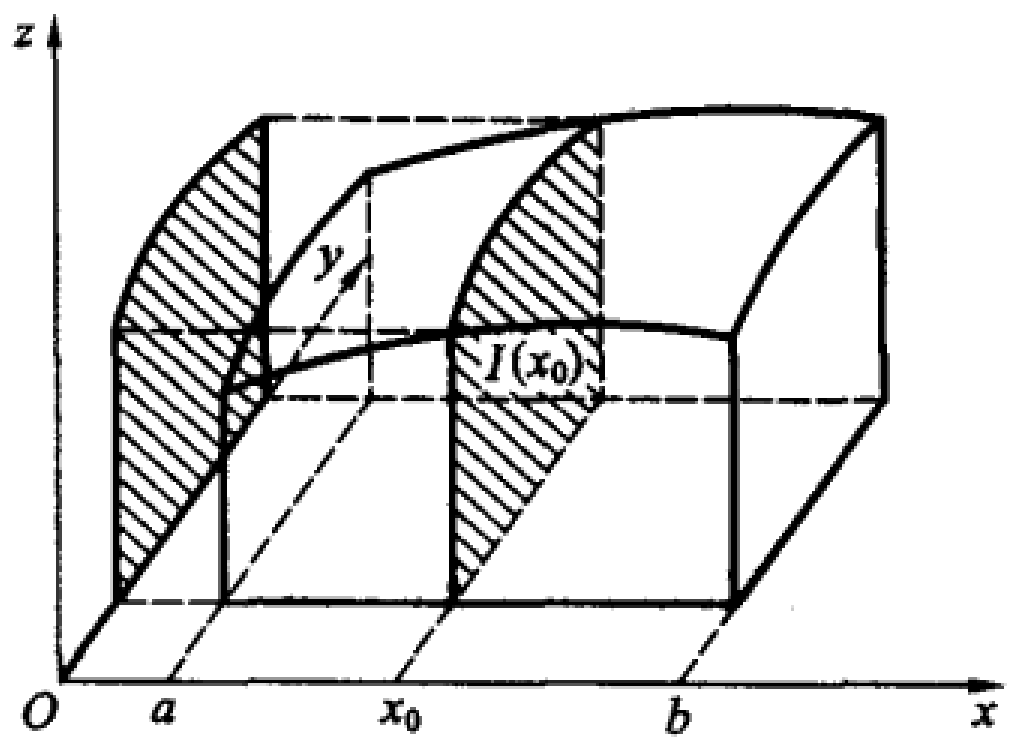
\includegraphics[width=0.45\textwidth]{work/figures/fig19-1}\caption{\relax}\label{fig:19-1}
\end{figure}

\begin{theorem}[积分号下求导数]\label{thm:19-2}
设 $f(x,y)$ 和 $f_{x}(x,y)$ 在 $[a,b]\times[c,d]$ 上连续，则 $I(x)$ 在 $[a,b]$ 有连续的导函数，且
\[
I^{\prime}(x)=\int_{c}^{d}f_{x}(x,y)\dd y.
\]
\end{theorem}

\begin{proof}
对任意 $x\in[a,b]$ 和 $x+\Delta x\in[a,b]$，由拉格朗日中值定理，存在 $\theta\in(0,1)$，使得
\[
\begin{aligned}
\frac{I(x+\Delta x)-I(x)}{\Delta x}&=\int_{c}^{d}\frac{f(x+\Delta x,y)-f(x,y)}{\Delta x}\dd y\\
&=\int_{c}^{d}f_{x}(x+\theta\Delta x,y)\dd y.
\end{aligned}
\]
由函数 $f_{x}(x,y)$ 在 $[a,b]\times[c,d]$ 连续，从而一致连续，即对任给的 $\varepsilon>0$，存在 $\delta>0$，只要 $|\Delta x|<\delta$，有
\[
|f_{x}(x+\theta\Delta x,y)-f_{x}(x,y)|<\frac{\varepsilon}{d-c}
\]
对 $y\in[c,d]$ 同时成立，因此
\[
\begin{aligned}
&\left|\frac{I(x+\Delta x)-I(x)}{\Delta x}-\int_{c}^{d}f_{x}(x,y)\dd y\right|\\
={}&\left|\int_{c}^{d}\left[f_{x}(x+\theta\Delta x,y)-f_{x}(x,y)\right]\dd y\right|\\
\leqslant{}&\int_{c}^{d}\left|f_{x}(x+\theta\Delta x,y)-f_{x}(x,y)\right|\dd y\\
<{}&\frac{\varepsilon}{d-c}\int_{c}^{d}\dd y=\varepsilon.
\end{aligned}
\]
故 $I(x)$ 在 $x$ 可导，且
\[
I^{\prime}(x)=\int_{c}^{d}f_{x}(x,y)\dd y.
\]
由 $x\in[a,b]$ 的任意性及定理 19.1 知，$I(x)$ 在 $[a,b]$ 有连续的导函数，且上式成立．定理~\ref{thm:19-2} 证完．
\end{proof}

定理 19.2 的结论又可写为
\[
\frac{\dd}{\dd x}\int_{c}^{d}f(x,y)\dd y=\int_{c}^{d}f_{x}(x,y)\dd y=\int_{c}^{d}\frac{\partial}{\partial x}f(x,y)\dd y.
\]
这说明，在定理的条件下，求导和求积分可交换次序．我们也常说可在积分号下求导数．

\begin{example}\label{ex:19-1-1}
求 $I(\theta)=\int_{0}^{\pi}\ln(1+\theta\cos x)\dd x$，其中 $|\theta|<1$．
\end{example}

\begin{proof}[解]
对任意 $|\theta|<1$，存在 $b$ 使得 $|\theta|<b<1$．于是
\[
f(x,\theta)=\ln(1+\theta\cos x),\quad f_{\theta}(x,\theta)=\frac{\cos x}{1+\theta\cos x}
\]
都在 $[0,\pi]\times[-b,b]$ 连续，由定理 19.2 得
\[
I^{\prime}(\theta)=\int_{0}^{\pi}\frac{\cos x}{1+\theta\cos x}\dd x.
\]
当 $\theta\neq 0$ 时
\[
\begin{aligned}
I^{\prime}(\theta)&=\frac{1}{\theta}\int_{0}^{\pi}\left(1-\frac{1}{1+\theta\cos x}\right)\dd x\\
&=\frac{\pi}{\theta}-\frac{1}{\theta}\int_{0}^{\pi}\frac{\dd x}{1+\theta\cos x}.
\end{aligned}
\]
令 $\tan\dfrac{x}{2}=t$，则
\[
\begin{aligned}
\int_{0}^{\pi}\frac{\dd x}{1+\theta\cos x}&=\int_{0}^{+\infty}\frac{1}{1+\theta\dfrac{1-t^{2}}{1+t^{2}}}\cdot\frac{2}{1+t^{2}}\dd t\\
&=\int_{0}^{+\infty}\frac{2\dd t}{(1+\theta)+(1-\theta)t^{2}}=\left.\frac{2}{\sqrt{1-\theta^{2}}}\arctan\sqrt{\frac{1-\theta}{1+\theta}}\,t\right|_{0}^{+\infty}\\
&=\frac{\pi}{\sqrt{1-\theta^{2}}}.
\end{aligned}
\]
因此
\[
I^{\prime}(\theta)=\frac{\pi}{\theta}-\frac{\pi}{\theta\sqrt{1-\theta^{2}}}=\frac{-\theta\pi}{\sqrt{1-\theta^{2}}\left(1+\sqrt{1-\theta^{2}}\right)},
\]
积分得
\[
\begin{aligned}
I(\theta)&=\int\frac{-\theta\pi\dd\theta}{\sqrt{1-\theta^{2}}\left(1+\sqrt{1-\theta^{2}}\right)}\\
&=\pi\int\frac{\dd\sqrt{1-\theta^{2}}}{1+\sqrt{1-\theta^{2}}}\\
&=\pi\ln\left(1+\sqrt{1-\theta^{2}}\right)+C,\ \theta\in[-b,b],\ \theta\neq 0.
\end{aligned}
\]
又由 $I(0)=0$ 及 $I(\theta)$ 的连续性得 $C=-\pi\ln 2$，因此
\[
I(\theta)=\pi\ln\frac{1+\sqrt{1-\theta^{2}}}{2},\quad|\theta|<1.
\]
\end{proof}

我们发现，用含参变量积分给出的 $I(\theta)$，原来是一个初等函数．这一点，用一元函数的积分知识是不容易看出来的．我们用了含参变量积分的理论（积分号下求导数），才把它计算出来．

\begin{example}\label{ex:19-1-2}
计算定积分
\[
I=\int_{0}^{1}\frac{\ln(1+x)}{1+x^{2}}\dd x.
\]
\end{example}

\begin{proof}[解]
这个积分并不带参变量，但被积函数的原函数不能用初等函数表示．为此，引入参变量，考虑含参变量积分
\[
I(\alpha)=\int_{0}^{1}\frac{\ln(1+\alpha x)}{1+x^{2}}\dd x,\quad\alpha\in[0,1].
\]
我们将通过积分号下求导数，再求出 $I=I(1)$．记
\[
f(x,\alpha)=\frac{\ln(1+\alpha x)}{1+x^{2}},
\]
则
\[
f_{\alpha}(x,\alpha)=\frac{x}{(1+x^{2})(1+\alpha x)}=\frac{1}{1+\alpha^{2}}\left(\frac{\alpha+x}{1+x^{2}}-\frac{\alpha}{1+\alpha x}\right)
\]
它们都在 $[0,1]\times[0,1]$ 上连续，根据定理 19.2，有
\[
\begin{aligned}
I^{\prime}(\alpha)&=\int_{0}^{1}f_{\alpha}(x,\alpha)\dd x\\
&=\int_{0}^{1}\frac{1}{1+\alpha^{2}}\left(\frac{\alpha+x}{1+x^{2}}-\frac{\alpha}{1+\alpha x}\right)\dd x\\
&=\frac{1}{1+\alpha^{2}}\left[\alpha\arctan x+\frac{1}{2}\ln(1+x^{2})-\ln(1+\alpha x)\right]\bigg|_{0}^{1}\\
&=\frac{1}{1+\alpha^{2}}\left[\frac{\pi}{4}\alpha+\frac{1}{2}\ln 2-\ln(1+\alpha)\right].
\end{aligned}
\]
注意到 $I(0)=0$，故
\[
\begin{aligned}
I(1)&=I(1)-I(0)=\int_{0}^{1}I^{\prime}(\alpha)\dd\alpha\\
&=\int_{0}^{1}\frac{1}{1+\alpha^{2}}\left[\frac{\pi}{4}\alpha+\frac{1}{2}\ln 2-\ln(1+\alpha)\right]\dd\alpha\\
&=\left[\frac{\pi}{8}\ln(1+\alpha^{2})+\frac{1}{2}\ln 2\arctan\alpha\right]\bigg|_{0}^{1}-\int_{0}^{1}\frac{\ln(1+\alpha)}{1+\alpha^{2}}\dd\alpha\\
&=\frac{\pi}{8}\ln 2+\frac{\pi}{8}\ln 2-I(1)=\frac{\pi}{4}\ln 2-I(1),
\end{aligned}
\]
从而
\[
I=I(1)=\frac{\pi}{8}\ln 2.
\]
\end{proof}

下面我们进一步考虑含参变量积分的积分限也依赖于参数 $x$ 的情形．为此先考虑函数
\[
I(x,u)=\int_{c}^{u}f(x,y)\dd y
\]
的性质．

\begin{theorem}\label{thm:19-3}
设函数 $f(x,y)$ 在矩形区域 $[a,b]\times[c,d]$ 上连续，
\[
I(x,u)=\int_{c}^{u}f(x,y)\dd y,
\]
则（1）$I(x,u)$ 在 $[a,b]\times[c,d]$ 上连续；

（2）若 $f_{x}(x,y)$ 在 $[a,b]\times[c,d]$ 上连续，则 $I(x,u)$ 在 $[a,b]\times[c,d]$ 对各变元有连续偏导数．
\end{theorem}

\begin{proof}
（1）对任意 $(x_{0},u_{0})$，$(x,u)\in[a,b]\times[c,d]$，则
\[
\begin{aligned}
&|I(x,u)-I(x_{0},u_{0})|=\left|\int_{c}^{u}f(x,y)\dd y-\int_{c}^{u_{0}}f(x_{0},y)\dd y\right|\\
={}&\left|\int_{c}^{u_{0}}\left[f(x,y)-f(x_{0},y)\right]\dd y+\int_{u_{0}}^{u}f(x,y)\dd y\right|.
\end{aligned}
\]
由 $f(x,y)$ 在 $[a,b]\times[c,d]$ 上连续，因而有界且一致连续，知存在 $M>0$，使
\[
|f(x,y)|\leqslant M,\quad(x,y)\in[a,b]\times[c,d],
\]
且对任给的 $\varepsilon>0$，存在 $\delta_{1}>0$，对任意的 $(x_{1},y_{1})$，$(x_{2},y_{2})\in[a,b]\times[c,d]$，只要 $|x_{1}-x_{2}|<\delta_{1}$ 和 $|y_{1}-y_{2}|<\delta_{1}$，就有
\[
|f(x_{1},y_{1})-f(x_{2},y_{2})|<\frac{\varepsilon}{2(d-c)}.
\]
取 $\delta=\min\left(\delta_{1},\dfrac{\varepsilon}{2M}\right)$，则当 $|x-x_{0}|<\delta$，$|u-u_{0}|<\delta$ 时，有
\[
\begin{aligned}
&|I(x,u)-I(x_{0},u_{0})|\\
\leqslant{}&\int_{c}^{u_{0}}|f(x,y)-f(x_{0},y)|\dd y+M\left|\int_{u_{0}}^{u}\dd y\right|\\
<{}&\frac{\varepsilon}{2(d-c)}(u_{0}-c)+M\frac{\varepsilon}{2M}\leqslant\frac{\varepsilon}{2}+\frac{\varepsilon}{2}=\varepsilon.
\end{aligned}
\]
即 $I(x,u)$ 在 $(x_{0},u_{0})$ 点连续．由 $(x_{0},u_{0})\in[a,b]\times[c,d]$ 的任意性，便证得 $I(x,u)$ 在 $[a,b]\times[c,d]$ 上连续．

（2）由微积分基本定理，$I$ 对 $u$ 有连续的偏导数
\[
\frac{\partial I}{\partial u}=f(x,u).
\]
又由定理 19.2，$I$ 对 $x$ 也有连续的偏导数
\[
\frac{\partial I}{\partial x}=\int_{c}^{u}f_{x}(x,y)\dd y.
\]
这就是所要证明的，定理~\ref{thm:19-3} 证完．
\end{proof}

利用定理 19.3 及复合函数的连续性与求导数的链式法则，立即可得下面两个定理．

\begin{theorem}\label{thm:19-4}
设函数 $f(x,y)$ 在 $[a,b]\times[c,d]$ 上连续，$c(x)$，$d(x)$ 都在 $[a,b]$ 上连续，并且当 $x\in[a,b]$ 时，有
\[
c\leqslant c(x),\ d(x)\leqslant d,
\]
则
\[
F(x)=\int_{c(x)}^{d(x)}f(x,y)\dd y
\]
在 $[a,b]$ 连续．
\end{theorem}

\begin{proof}
令 $u=d(x)$，$v=c(x)$，$I(x,u)=\int_{c}^{u}f(x,y)\dd y$．根据定理 19.3，
\[
\int_{v}^{u}f(x,y)\dd y=\int_{c}^{u}f(x,y)\dd y-\int_{c}^{v}f(x,y)\dd y=I(x,u)-I(x,v)
\]
在 $[a,b]\times[c,d]\times[c,d]$ 上连续．由复合函数的连续性知
\[
F(x)=I(x,d(x))-I(x,c(x))
\]
在 $[a,b]$ 连续．定理~\ref{thm:19-4} 证完．
\end{proof}

\begin{theorem}\label{thm:19-5}
设函数 $f(x,y)$，$f_{x}(x,y)$ 都在 $[a,b]\times[c,d]$ 上连续，又 $c^{\prime}(x)$ 和 $d^{\prime}(x)$ 在 $[a,b]$ 存在，且当 $x\in[a,b]$ 时，有
\[
c\leqslant c(x),\ d(x)\leqslant d,
\]
则
\[
F(x)=\int_{c(x)}^{d(x)}f(x,y)\dd y
\]
在 $[a,b]$ 可导，且
\[
F^{\prime}(x)=\int_{c(x)}^{d(x)}f_{x}(x,y)\dd y+f(x,d(x))d^{\prime}(x)-f(x,c(x))c^{\prime}(x).
\]
\end{theorem}

\begin{proof}
令
\[
I(x,u)=\int_{c}^{u}f(x,y)\dd y,\quad H(x,u,v)=\int_{v}^{u}f(x,y)\dd y.
\]
则 $H(x,u,v)=I(x,u)-I(x,v)$．由定理 19.3，$H$ 对各变元有连续的偏导数．又 $c(x)$，$d(x)$ 在 $[a,b]$ 可导，且当 $x\in[a,b]$ 时，
\[
c\leqslant c(x),\ d(x)\leqslant d,
\]
故由复合函数求导数的链式法则，$F(x)=H(x,c(x),d(x))$ 在 $[a,b]$ 可导，且
\[
\begin{aligned}
F^{\prime}(x)&=\frac{\partial H}{\partial x}+\frac{\partial H}{\partial u}d^{\prime}(x)+\frac{\partial H}{\partial v}c^{\prime}(x)\\
&=\int_{c(x)}^{d(x)}f_{x}(x,y)\dd y+f(x,d(x))d^{\prime}(x)-f(x,c(x))c^{\prime}(x).
\end{aligned}
\]
定理~\ref{thm:19-5} 证完．
\end{proof}

其实，定理 19.4、19.5 也可以不用定理 19.3 而直接证明，作为一个练习，请读者把它们写出来．

\begin{example}\label{ex:19-1-3}
设 $F(x)=\int_{x}^{x^{2}}\dfrac{\sin xy}{y}\dd y$，求 $F^{\prime}(x)$．
\end{example}

\begin{proof}[解]
这个积分是积不出来的，但用定理 19.5 有
\[
\begin{aligned}
F^{\prime}(x)&=\int_{x}^{x^{2}}\cos xy\dd y+2x\left(\frac{\sin x^{3}}{x^{2}}\right)-\frac{\sin x^{2}}{x}\\
&=\frac{1}{x}\sin xy\bigg|_{x}^{x^{2}}+\frac{2\sin x^{3}}{x}-\frac{\sin x^{2}}{x}\\
&=\frac{3\sin x^{3}-2\sin x^{2}}{x}.
\end{aligned}
\]
\end{proof}

\begin{example}\label{ex:19-1-4}
设 $f(x)$ 在 $x=0$ 的某邻域内连续，则微分方程
\[
\begin{cases}
y^{(n)}(x)=f(x),\\
y(0)=0,\quad y^{\prime}(0)=0,\quad\cdots,\quad y^{(n-1)}(0)=0
\end{cases}
\]
的解在 $x=0$ 附近可表示成
\[
y(x)=\frac{1}{(n-1)!}\int_{0}^{x}(x-t)^{n-1}f(t)\dd t,
\]
其中 $n$ 是任意正整数．
\end{example}

\begin{proof}
利用定理 19.5，则
\[
\begin{aligned}
y^{\prime}(x)&=\frac{1}{(n-1)!}\int_{0}^{x}(n-1)(x-t)^{n-2}f(t)\dd t\\
&\quad+\frac{1}{(n-1)!}(x-x)^{n-1}f(x)\\
&=\frac{1}{(n-2)!}\int_{0}^{x}(x-t)^{n-2}f(t)\dd t.
\end{aligned}
\]
一般地有
\[
y^{(k)}(x)=\frac{1}{(n-k-1)!}\int_{0}^{x}(x-t)^{n-k-1}f(t)\dd t,
\]
从而
\[
y^{(n-1)}(x)=\int_{0}^{x}f(t)\dd t,
\]
\[
y^{(n)}(x)=f(x).
\]
显然
\[
y(0)=y^{\prime}(0)=\cdots=y^{(k)}(0)=\cdots=y^{(n-1)}(0)=0.
\]
\end{proof}

最后我们来讨论含参变量积分 $I(x)=\int_{c}^{d}f(x,y)\dd y$ 的积分问题．如果 $I(x)$ 在 $[a,b]$ 可积，通常把它在 $[a,b]$ 的积分写为
\[
\int_{a}^{b}I(x)\dd x=\int_{a}^{b}\left[\int_{c}^{d}f(x,y)\dd y\right]\dd x=\int_{a}^{b}\dd x\int_{c}^{d}f(x,y)\dd y,
\]
称之为先对 $y$ 后对 $x$ 的累次积分．

\begin{theorem}[积分交换次序]\label{thm:19-6}
设 $f(x,y)$ 在 $[a,b]\times[c,d]$ 上连续，
\[
I(x)=\int_{c}^{d}f(x,y)\dd y,
\]
则
\[
\int_{a}^{b}I(x)\dd x=\int_{c}^{d}\dd y\int_{a}^{b}f(x,y)\dd x,
\]
即
\[
\int_{a}^{b}\dd x\int_{c}^{d}f(x,y)\dd y=\int_{c}^{d}\dd y\int_{a}^{b}f(x,y)\dd x.
\]
\end{theorem}

\begin{proof}
由定理 19.1，$I(x)$ 在 $[a,b]$ 连续，因而是可积的，令
\[
I_{1}(u)=\int_{a}^{u}\dd x\int_{c}^{d}f(x,y)\dd y,\ u\in[a,b],
\]
\[
I_{2}(u)=\int_{c}^{d}\dd y\int_{a}^{u}f(x,y)\dd x,\ u\in[a,b].
\]
由定理 19.1 知，$\displaystyle\int_{c}^{d}f(x,y)\dd y$ 在 $[a,b]$ 连续，因此 $I_{1}(u)$ 在 $[a,b]$ 可导，且
\[
I_{1}^{\prime}(u)=\int_{c}^{d}f(u,y)\dd y,
\]
又由定理 19.3 知，$\displaystyle\int_{a}^{u}f(x,y)\dd x$ 关于变量 $y$，$u$ 二元连续，其关于 $u$ 的偏导数 $f(u,y)$ 也是连续的，从而由定理 19.2 知，$I_{2}(u)$ 在 $[a,b]$ 可导，且
\[
I_{2}^{\prime}(u)=\int_{c}^{d}\frac{\partial}{\partial u}\int_{a}^{u}f(x,y)\dd x\dd y=\int_{c}^{d}f(u,y)\dd y.
\]
这就证明了
\[
I_{1}^{\prime}(u)=I_{2}^{\prime}(u),\ u\in[a,b].
\]
因此
\[
I_{1}(u)=I_{2}(u)+c,\quad u\in[a,b].
\]
令 $u=a$，由 $I_{1}(a)=I_{2}(a)=0$ 推得 $c=0$．故
\[
I_{1}(u)=I_{2}(u),\quad u\in[a,b].
\]
令 $u=b$，即得
\[
\int_{a}^{b}\dd x\int_{c}^{d}f(x,y)\dd y=\int_{c}^{d}\dd y\int_{a}^{b}f(x,y)\dd x.
\]
定理~\ref{thm:19-6} 证完．
\end{proof}

定理 19.6 说明：在被积函数二元连续的条件下，两个累次积分可以交换次序．

\begin{example}\label{ex:19-1-5}
用积分交换次序求解例 1，即求
\[
I(\theta)=\int_{0}^{\pi}\ln(1+\theta\cos x)\dd x,
\]
其中 $|\theta|<1$．
\end{example}

\begin{proof}[解]
显然 $I(\theta)=\displaystyle\int_{0}^{\pi}\dd x\int_{0}^{\theta}\frac{\cos x}{1+y\cos x}\dd y$．令
\[
f(x,y)=\frac{\cos x}{1+y\cos x},
\]
因为 $f(x,y)$ 在 $[0,\pi]\times[0,\theta]$ 上连续，所以积分可交换次序，
\[
I(\theta)=\int_{0}^{\theta}\dd y\int_{0}^{\pi}\frac{\cos x}{1+y\cos x}\dd x.
\]
用变量代换，在例 1 中已求出
\[
\int_{0}^{\pi}\frac{\cos x}{1+y\cos x}\dd x=\frac{-y\pi}{\sqrt{1-y^{2}}\left(1+\sqrt{1-y^{2}}\right)},
\]
因此
\[
\begin{aligned}
I(\theta)&=\int_{0}^{\theta}\frac{-y\pi}{\sqrt{1-y^{2}}\left(1+\sqrt{1-y^{2}}\right)}\dd y\\
&=\pi\int_{0}^{\theta}\frac{\dd\sqrt{1-y^{2}}}{1+\sqrt{1-y^{2}}}=\pi\ln\left(1+\sqrt{1-y^{2}}\right)\bigg|_{0}^{\theta}\\
&=\pi\ln\frac{1+\sqrt{1-\theta^{2}}}{2}.
\end{aligned}
\]
\end{proof}

\begin{xiti}
\item 求下列极限：
\begin{ziti}
\item $\lim\limits_{a\to 0}\displaystyle\int_{-1}^{1}\sqrt{x^{2}+a^{2}}\dd x$；
\item $\lim\limits_{a\to 0}\displaystyle\int_{0}^{2}x^{2}\cos ax\dd x$；
\item $\lim\limits_{a\to 0}\displaystyle\int_{a}^{1+a}\frac{\dd x}{1+x^{2}+a^{2}}$．
\end{ziti}
\item 求 $F^{\prime}(x)$，其中：
\begin{ziti}
\item $F(x)=\displaystyle\int_{x}^{x^{2}}\mathrm{e}^{-xy^{2}}\dd y$；
\item $F(x)=\displaystyle\int_{\sin x}^{\cos x}\mathrm{e}^{x\sqrt{1-y^{2}}}\dd y$；
\item $F(x)=\displaystyle\int_{a+x}^{b+x}\frac{\sin(xy)}{y}\dd y$；
\item $F(x)=\displaystyle\int_{0}^{x}\left[\int_{t^{2}}^{x}f(t,s)\dd s\right]\dd t$．
\end{ziti}
\item 设 $f(x)$ 为连续函数，$h>0$，
\[
F(x)=\int_{0}^{h}\left[\int_{0}^{h}f(x+\xi+\eta)\dd\eta\right]\dd\xi,
\]
求 $F^{\prime\prime}(x)$．
\item 研究函数
\[
F(y)=\int_{0}^{1}\frac{yf(x)}{x^{2}+y^{2}}\dd x
\]
的连续性，其中 $f(x)$ 是 $[0,1]$ 上连续且为正的函数．
\item 应用积分号下求导法求下列积分：
\begin{ziti}
\item $\displaystyle\int_{0}^{\frac{\pi}{2}}\ln(a^{2}-\sin^{2}x)\dd x$ $(a>1)$；
\item $\displaystyle\int_{0}^{\pi}\ln(1-2a\cos x+a^{2})\dd x$ $(|a|<1)$；
\item $\displaystyle\int_{0}^{\frac{\pi}{2}}\ln(a^{2}\sin^{2}x+b^{2}\cos^{2}x)\dd x$ $(a,b\neq 0)$；
\item $\displaystyle\int_{0}^{\frac{\pi}{2}}\frac{\arctan(a\tan x)}{\tan x}\dd x$ $(|a|<1)$．
\end{ziti}
\item 应用积分交换次序求下列积分：
\begin{ziti}
\item $\displaystyle\int_{0}^{1}\frac{x^{b}-x^{a}}{\ln x}\dd x$ $(a>0,\ b>0)$；
\item $\displaystyle\int_{0}^{1}\sin\left(\ln\frac{1}{x}\right)\frac{x^{b}-x^{a}}{\ln x}\dd x$ $(a>0,\ b>0)$．
\end{ziti}
\item 设 $f$ 为可微函数，试求下列函数的二阶导数：
\begin{ziti}
\item $F(x)=\displaystyle\int_{0}^{x}(x+y)f(y)\dd y$；
\item $F(x)=\displaystyle\int_{a}^{b}f(y)\left|x-y\right|\dd y$ $(a<b)$．
\end{ziti}
\item 证明：$\displaystyle\int_{0}^{1}\dd x\int_{0}^{1}\frac{x^{2}-y^{2}}{(x^{2}+y^{2})^{2}}\dd y\neq\int_{0}^{1}\dd y\int_{0}^{1}\frac{x^{2}-y^{2}}{(x^{2}+y^{2})^{2}}\dd x$．
\item 设 $F(y)=\displaystyle\int_{0}^{1}\ln\sqrt{x^{2}+y^{2}}\dd x$，问是否成立
\[
F^{\prime}(0)=\int_{0}^{1}\frac{\partial}{\partial y}\ln\sqrt{x^{2}+y^{2}}\bigg|_{y=0}\dd x.
\]
\item 设
\[
F(x)=\int_{0}^{2\pi}\mathrm{e}^{x\cos\theta}\cos(x\sin\theta)\dd\theta,
\]
求证 $F(x)\equiv 2\pi$．
\item 设 $f(x)$ 为两次可微函数，$\varphi(x)$ 为可微函数，证明函数
\[
u(x,t)=\frac{1}{2}\left[f(x-at)+f(x+at)\right]+\frac{1}{2a}\int_{x-at}^{x+at}\varphi(z)\dd z
\]
满足弦振动方程
\[
\frac{\partial^{2}u}{\partial t^{2}}=a^{2}\frac{\partial^{2}u}{\partial x^{2}}
\]
及初始条件
\[
u(x,0)=f(x),\quad u_{t}(x,0)=\varphi(x).
\]
\end{xiti}

\section{含参变量的广义积分}

\subsection{一致收敛}

广义积分有两种，一种是无穷限积分，即积分区间为无穷的情形，另一种为瑕积分，即积分区间虽然是有穷的，但被积函数在积分区间内无界．当含参变量的积分是广义积分时，就称为含参变量的广义积分．它自然包括两种．

设 $f(x,y)$ 定义在 $[a,b]\times[c,+\infty)$，则
\[
I(x)=\int_{c}^{+\infty}f(x,y)\dd y
\]
为无穷限的含参变量积分，其中 $x$ 是参变量，$y$ 是积分变量．如果 $f(x,y)$ 定义在 $[a,b]\times[c,d]$，且对任意 $x\in[a,b]$ 以及 $\eta>0$ 充分小，$f(x,y)$ 对 $y$ 在 $[c,d-\eta]$ 可积，但在 $[d-\eta,d)$ 无界，则
\[
J(x)=\int_{c}^{d}f(x,y)\dd y
\]
是含参变量的瑕积分．根据广义积分的定义
\[
\int_{c}^{+\infty}f(x,y)\dd y=\lim_{A\to+\infty}\int_{c}^{A}f(x,y)\dd y,
\]
\[
\int_{c}^{d}f(x,y)\dd y=\lim_{\eta\to 0^{+}}\int_{c}^{d-\eta}f(x,y)\dd y,
\]
它们都是含参变量正常积分的极限，这与函数项级数
\[
\sum_{k=1}^{\infty}u_{k}(x),\ x\in[a,b]
\]
十分类似，它是有限和（部分和）的极限
\[
\sum_{k=1}^{\infty}u_{k}(x)=\lim_{n\to\infty}\sum_{k=1}^{n}u_{k}(x).
\]
唯一的差别是，在级数的情形，极限是对离散量 $n\to\infty$ 取的，而在含参变量广义积分的情形，极限是对连续量 $A\to+\infty$ 或 $\eta\to 0^{+}$ 取的．回忆函数项级数理论，我们研究过它的两个基本问题：（1）收敛区域；（2）和函数在收敛区域的分析性质（连续性、可微性、可积性等）．对含参变量的广义积分，同样地有两个问题，但收敛区域的问题，实际上已在第十一章中讲述过．因此本章主要讨论由广义积分表示的函数的分析性质问题．

回忆函数项级数的情形，在和函数分析性质的研究中，一致收敛的概念起了关键的作用．通过一致收敛，把无穷和的性质化为有限和的研究．在含参变量广义积分的讨论中，我们也引入一致收敛的概念，它把广义积分的问题化归为含参变量的正常积分，而后者在本章 §1 中已讨论过．本章主要讨论无穷限的情形，但所有的结果都可平行地推广到瑕积分的情形．

\begin{definition}\label{def:19-1}
设 $f(x,y)$ 定义在 $[a,b]\times[c,+\infty)$，且对任意 $x\in[a,b]$，无穷积分
\[
I(x)=\int_{c}^{+\infty}f(x,y)\dd y
\]
收敛．若对任意的 $\varepsilon>0$，存在 $A_{0}>c$，当 $A>A_{0}$ 时，有
\[
\left|\int_{c}^{A}f(x,y)\dd y-I(x)\right|<\varepsilon
\]
或
\[
\left|\int_{A}^{+\infty}f(x,y)\dd y\right|<\varepsilon
\]
对 $x\in[a,b]$ 都成立，则称含参变量的广义积分 $\displaystyle\int_{c}^{+\infty}f(x,y)\dd y$ 在 $[a,b]$ 一致收敛．
\end{definition}

显然，定义中的区间 $[a,b]$ 可代之以开区间、半开区间、无穷区间等等．

\begin{example}\label{ex:19-2-1}
证明含参变量广义积分 $\displaystyle\int_{0}^{+\infty}x\mathrm{e}^{-xy}\dd y$

（1）在 $[a,+\infty)$ 一致收敛，其中 $a>0$；

（2）在 $(0,+\infty)$ 不一致收敛．
\end{example}

\begin{proof}
（1）因为
\[
\int_{A}^{+\infty}x\mathrm{e}^{-xy}\dd y=-\left.\mathrm{e}^{-xy}\right|_{A}^{+\infty}=\mathrm{e}^{-xA}\leqslant\mathrm{e}^{-aA},\ x\geqslant a,
\]
而 $\lim\limits_{A\to+\infty}\mathrm{e}^{-aA}=0$，所以对任给的 $\varepsilon>0$，存在 $A_{0}>0$，当 $A>A_{0}$ 时有 $\mathrm{e}^{-aA}<\varepsilon$，从而当 $A>A_{0}$ 时，对任意的 $x\geqslant a$，有
\[
\left|\int_{A}^{+\infty}x\mathrm{e}^{-xy}\dd y\right|\leqslant\mathrm{e}^{-aA}<\varepsilon.
\]
这就证明了 $\displaystyle\int_{0}^{+\infty}x\mathrm{e}^{-xy}\dd y$ 在 $[a,+\infty)$ 一致收敛．

（2）要证存在 $\varepsilon_{0}>0$，对任意的 $A_{0}>0$，存在 $A>A_{0}$ 和 $x_{0}\in(0,+\infty)$，使得
\[
\left|\int_{A}^{+\infty}x_{0}\mathrm{e}^{-x_{0}y}\dd y\right|\geqslant\varepsilon_{0}.
\]
从
\[
\int_{A}^{+\infty}x\mathrm{e}^{-xy}\dd y=\mathrm{e}^{-xA}
\]
易知，只要取 $\varepsilon_{0}=\dfrac{1}{2}\mathrm{e}^{-1}$，$x_{0}=\dfrac{1}{A}\in(0,+\infty)$，就有
\[
\int_{A}^{+\infty}x_{0}\mathrm{e}^{-x_{0}y}\dd y=\mathrm{e}^{-1}>\varepsilon_{0}.
\]
也就是说，存在 $\varepsilon_{0}=\dfrac{1}{2}\mathrm{e}^{-1}>0$，对任意 $A_{0}>0$，存在 $A>A_{0}$ 和 $x_{0}=\dfrac{1}{A}\in(0,+\infty)$，使得
\[
\left|\int_{A}^{+\infty}x_{0}\mathrm{e}^{-x_{0}y}\dd y\right|=\mathrm{e}^{-1}>\frac{1}{2}\mathrm{e}^{-1}=\varepsilon_{0}.
\]
因此 $\displaystyle\int_{0}^{+\infty}x\mathrm{e}^{-xy}\dd y$ 在 $(0,+\infty)$ 不一致收敛．
\end{proof}

显然，$\displaystyle\int_{0}^{+\infty}x\mathrm{e}^{-xy}\dd y$ 在 $[0,+\infty)$ 是收敛的．当 $x>0$ 时
\[
\int_{0}^{+\infty}x\mathrm{e}^{-xy}\dd y=-\left.\mathrm{e}^{-xy}\right|_{0}^{+\infty}=1,
\]
而当 $x=0$ 时，被积函数恒等于 $0$，故
\[
I(x)=\int_{0}^{+\infty}x\mathrm{e}^{-xy}\dd y=\begin{cases}
0,&x=0,\\
1,&x\in(0,+\infty).
\end{cases}
\]
例子表明，尽管被积函数 $f(x,y)=x\mathrm{e}^{-xy}$ 在 $[0,+\infty)\times[0,+\infty)$ 连续，但 $I(x)$ 在 $x=0$ 不连续．读者可能已意识到，其原因是积分在包含 $x=0$ 的区间是不一致收敛的．后文将说明事实的确如此．

为便于判别一致收敛性，下面给出一致收敛的柯西准则和几个常用的判别法，它们的证明和级数的相仿，请读者把证明写出来．其中 $[a,b]$ 区间可代之以开区间、半开区间、无穷区间等等．

\begin{theorem}[一致收敛的柯西准则]\label{thm:19-7}
含参变量的广义积分 $\displaystyle\int_{c}^{+\infty}f(x,y)\dd y$ 在 $[a,b]$ 一致收敛的充要条件是对任给的 $\varepsilon>0$，存在正数 $A_{0}>c$，当 $A^{\prime},A^{\prime\prime}>A_{0}$ 时，对任意的 $x\in[a,b]$，有
\[
\left|\int_{A^{\prime}}^{A^{\prime\prime}}f(x,y)\dd y\right|<\varepsilon.
\]
\end{theorem}

\begin{theorem}[魏尔斯特拉斯判别法，或 $M$ 判别法，或控制收敛判别法]\label{thm:19-8}
设存在函数 $M(y)$ 与常数 $B>c$，使得当 $y\geqslant B$ 与 $x\in[a,b]$ 时，有
\[
|f(x,y)|\leqslant M(y),
\]
而广义积分 $\displaystyle\int_{c}^{+\infty}M(y)\dd y$ 是收敛的，则 $\displaystyle\int_{c}^{+\infty}f(x,y)\dd y$ 在 $[a,b]$ 一致收敛．
\end{theorem}

\begin{theorem}[狄利克雷判别法]\label{thm:19-9}
设（1）含参变量的正常积分 $\displaystyle\int_{c}^{A}f(x,y)\dd y$ 在 $A\geqslant c$ 与 $x\in[a,b]$ 有界，即存在 $M>0$，对任意 $A\geqslant c$ 及任意 $x\in[a,b]$，有
\[
\left|\int_{c}^{A}f(x,y)\dd y\right|\leqslant M;
\]

（2）对每个固定的 $x\in[a,b]$，函数 $g(x,y)$ 关于 $y$ 是单调的，且当 $y\to+\infty$ 时，$g(x,y)$ 在 $x\in[a,b]$ 一致地趋向于 $0$．则含参变量广义积分
\[
\int_{c}^{+\infty}f(x,y)g(x,y)\dd y
\]
在 $[a,b]$ 一致收敛．
\end{theorem}

\begin{theorem}[阿贝尔判别法]\label{thm:19-10}
设（1）$\displaystyle\int_{c}^{+\infty}f(x,y)\dd y$ 在 $[a,b]$ 一致收敛；

（2）对每一个固定的 $x\in[a,b]$，函数 $g(x,y)$ 关于 $y$ 单调，且 $g(x,y)$ 在 $x\in[a,b]$，$y\geqslant c$ 有界．则含参变量广义积分
\[
\int_{c}^{+\infty}f(x,y)g(x,y)\dd y
\]
在 $[a,b]$ 一致收敛．
\end{theorem}

\begin{example}\label{ex:19-2-2}
证明 $\displaystyle\int_{0}^{+\infty}\frac{\cos(xy)}{1+x^{2}}\dd x$ 在 $(-\infty,+\infty)$ 一致收敛．
\end{example}

\begin{proof}
用魏尔斯特拉斯判别法．由于
\[
\left|\frac{\cos(xy)}{1+x^{2}}\right|\leqslant\frac{1}{1+x^{2}}
\]
对 $y\in(-\infty,+\infty)$ 与 $x\in[0,+\infty)$ 成立，而广义积分 $\displaystyle\int_{0}^{+\infty}\frac{\dd x}{1+x^{2}}$ 收敛，因此 $\displaystyle\int_{0}^{+\infty}\frac{\cos(xy)}{1+x^{2}}\dd x$ 在 $(-\infty,+\infty)$ 一致收敛．
\end{proof}

\begin{example}\label{ex:19-2-3}
证明
\[
\int_{0}^{+\infty}\mathrm{e}^{-xy}\frac{\sin x}{x}\dd x
\]
在 $[0,+\infty)$ 一致收敛．
\end{example}

\begin{proof}
用阿贝尔判别法．已知 $\displaystyle\int_{0}^{+\infty}\frac{\sin x}{x}\dd x$ 收敛（第十一章 §1 例 9 已证明）．又对每一个 $y\in[0,+\infty)$，函数 $\mathrm{e}^{-xy}$ 关于 $x$ 是单调函数，且
\[
\left|\mathrm{e}^{-xy}\right|\leqslant 1,\quad x\in[0,+\infty),\ y\in[0,+\infty).
\]
由阿贝尔判别法知，$\displaystyle\int_{0}^{+\infty}\mathrm{e}^{-xy}\frac{\sin x}{x}\dd x$ 在 $[0,+\infty)$ 一致收敛．
\end{proof}

\subsection{含参变量广义积分的分析性质}

\begin{theorem}[积分号下取极限]\label{thm:19-11}
设 $f(x,y)$ 在 $[a,b]\times[c,+\infty)$ 上连续，若含参变量广义积分
\[
I(x)=\int_{c}^{+\infty}f(x,y)\dd y
\]
在 $[a,b]$ 上一致收敛，则 $I(x)$ 在 $[a,b]$ 连续．
\end{theorem}

\begin{proof}
对任意 $x$，$x+\Delta x\in[a,b]$，
\[
|I(x+\Delta x)-I(x)|=\left|\int_{c}^{+\infty}\left[f(x+\Delta x,y)-f(x,y)\right]\dd y\right|.
\]
由于 $\displaystyle\int_{c}^{+\infty}f(x,y)\dd y$ 在 $[a,b]$ 一致收敛，知对任意 $\varepsilon>0$，存在 $A_{0}>c$，当 $A>A_{0}$ 时，对任意的 $x\in[a,b]$，有
\[
\left|\int_{A}^{+\infty}f(x,y)\dd y\right|<\frac{\varepsilon}{4}.
\]
固定 $A>A_{0}$，已知 $\displaystyle\int_{c}^{A}f(x,y)\dd y$ 是 $x$ 在 $[a,b]$ 的连续函数，因此存在 $\delta>0$，只要 $|\Delta x|<\delta$，有
\[
\left|\int_{c}^{A}f(x+\Delta x,y)\dd y-\int_{c}^{A}f(x,y)\dd y\right|<\frac{\varepsilon}{2},
\]
从而
\[
\begin{aligned}
&|I(x+\Delta x)-I(x)|\\
\leqslant{}&\left|\int_{c}^{A}\left[f(x+\Delta x,y)-f(x,y)\right]\dd y\right|+\left|\int_{A}^{+\infty}\left[f(x+\Delta x,y)-f(x,y)\right]\dd y\right|\\
\leqslant{}&\left|\int_{c}^{A}f(x+\Delta x,y)\dd y-\int_{c}^{A}f(x,y)\dd y\right|+\left|\int_{A}^{+\infty}f(x+\Delta x,y)\dd y\right|+\left|\int_{A}^{+\infty}f(x,y)\dd y\right|\\
<{}&\frac{\varepsilon}{2}+\frac{\varepsilon}{4}+\frac{\varepsilon}{4}=\varepsilon.
\end{aligned}
\]
这就证明了 $I(x)$ 在 $[a,b]$ 连续．定理~\ref{thm:19-11} 证完．
\end{proof}

$I(x)$ 在 $[a,b]$ 连续，这等价于说，对任意 $x_{0}\in[a,b]$，有
\[
\lim_{x\to x_{0}}I(x)=I(x_{0}),
\]
即
\[
\lim_{x\to x_{0}}\int_{c}^{+\infty}f(x,y)\dd y=I(x_{0})=\int_{c}^{+\infty}f(x_{0},y)\dd y=\int_{c}^{+\infty}\lim_{x\to x_{0}}f(x,y)\dd y,
\]
也就是说，求极限可以取到积分号之内，或说在积分号下取极限．

\begin{theorem}[积分交换次序]\label{thm:19-12}
设 $f(x,y)$ 在 $[a,b]\times[c,+\infty)$ 上连续．若含参变量广义积分
\[
I(x)=\int_{c}^{+\infty}f(x,y)\dd y
\]
在 $[a,b]$ 上一致收敛，则
\[
\int_{a}^{b}I(x)\dd x=\int_{c}^{+\infty}\dd y\int_{a}^{b}f(x,y)\dd x,
\]
即
\[
\int_{a}^{b}\dd x\int_{c}^{+\infty}f(x,y)\dd y=\int_{c}^{+\infty}\dd y\int_{a}^{b}f(x,y)\dd x.
\]
\end{theorem}

\begin{proof}
由定理 19.11 知，$I(x)$ 在 $[a,b]$ 连续，故可积，即
\[
\int_{a}^{b}I(x)\dd x=\int_{a}^{b}\dd x\int_{c}^{+\infty}f(x,y)\dd y
\]
为确定的数．下面只要证
\[
\lim_{A\to+\infty}\int_{c}^{A}\dd y\int_{a}^{b}f(x,y)\dd x=\int_{a}^{b}I(x)\dd x.
\]
根据含参变量的正常积分的积分交换次序定理，有
\[
\begin{aligned}
&\left|\int_{c}^{A}\dd y\int_{a}^{b}f(x,y)\dd x-\int_{a}^{b}I(x)\dd x\right|\\
={}&\left|\int_{a}^{b}\dd x\int_{c}^{A}f(x,y)\dd y-\int_{a}^{b}I(x)\dd x\right|\\
\leqslant{}&\int_{a}^{b}\left|\int_{c}^{A}f(x,y)\dd y-I(x)\right|\dd x.
\end{aligned}
\]
因为 $\displaystyle\int_{c}^{+\infty}f(x,y)\dd y$ 在 $[a,b]$ 一致收敛，所以对任给的 $\varepsilon>0$，存在 $A_{0}>c$，当 $A>A_{0}$ 时，对所有的 $x\in[a,b]$ 有
\[
\left|\int_{c}^{A}f(x,y)\dd y-I(x)\right|<\frac{\varepsilon}{b-a},
\]
从而当 $A>A_{0}$ 时，
\[
\begin{aligned}
&\left|\int_{c}^{A}\dd y\int_{a}^{b}f(x,y)\dd x-\int_{a}^{b}I(x)\dd x\right|\\
\leqslant{}&\int_{a}^{b}\left|\int_{c}^{A}f(x,y)\dd y-I(x)\right|\dd x<\frac{\varepsilon}{b-a}\int_{a}^{b}\dd x=\varepsilon.
\end{aligned}
\]
定理~\ref{thm:19-12} 证完．
\end{proof}

\begin{theorem}[积分号下求导数]\label{thm:19-13}
设 $f(x,y)$ 和 $f_{x}(x,y)$ 都在 $[a,b]\times[c,+\infty)$ 上连续，若 $\displaystyle\int_{c}^{+\infty}f(x,y)\dd y$ 在 $[a,b]$ 上收敛，$\displaystyle\int_{c}^{+\infty}f_{x}(x,y)\dd y$ 在 $[a,b]$ 上一致收敛，则
\[
I(x)=\int_{c}^{+\infty}f(x,y)\dd y
\]
在 $[a,b]$ 可导，且
\[
I^{\prime}(x)=\int_{c}^{+\infty}f_{x}(x,y)\dd y,
\]
即
\[
\frac{\dd}{\dd x}\int_{c}^{+\infty}f(x,y)\dd y=\int_{c}^{+\infty}\frac{\partial}{\partial x}f(x,y)\dd y.
\]
\end{theorem}

\begin{proof}
令
\[
g(x)=\int_{c}^{+\infty}f_{x}(x,y)\dd y.
\]
根据定理 19.12，$g(x)$ 在 $[a,b]$ 可积，且对任意 $t\in[a,b]$ 有
\[
\begin{aligned}
\int_{a}^{t}g(x)\dd x&=\int_{a}^{t}\dd x\int_{c}^{+\infty}f_{x}(x,y)\dd y\\
&=\int_{c}^{+\infty}\dd y\int_{a}^{t}f_{x}(x,y)\dd x\\
&=\int_{c}^{+\infty}\left[f(t,y)-f(a,y)\right]\dd y\\
&=I(t)-I(a).
\end{aligned}
\]
由定理 19.11，$g(x)$ 在 $[a,b]$ 连续，故 $\displaystyle\int_{a}^{t}g(x)\dd x$ 在 $[a,b]$ 可导，从而 $I(t)$ 可导．两边对 $t$ 求导数得
\[
g(t)=I^{\prime}(t),
\]
即
\[
I^{\prime}(x)=g(x)=\int_{c}^{+\infty}f_{x}(x,y)\dd y.
\]
定理~\ref{thm:19-13} 证完．
\end{proof}

定理 19.11、19.12、19.13 分别对应于第十二章 §3 函数项级数的定理 12.9、12.11、12.12．读者不难看出，从定理的叙述到证明，它们都是类似的．

\begin{example}\label{ex:19-2-4}
求狄利克雷积分
\[
I=\int_{0}^{+\infty}\frac{\sin x}{x}\dd x.
\]
\end{example}

\begin{proof}[解]
与上节例 2 一样，这个积分本身不带参变量，但为了求出它，引入因子 $\mathrm{e}^{-xy}$ $(y\geqslant 0)$．考虑含参变量的广义积分
\[
I(y)=\int_{0}^{+\infty}\mathrm{e}^{-xy}\frac{\sin x}{x}\dd x,\quad y\geqslant 0.
\]
记
\[
f(x,y)=\mathrm{e}^{-xy}\frac{\sin x}{x},
\]
这时
\[
f_{y}(x,y)=-\mathrm{e}^{-xy}\sin x.
\]
它们都在 $[0,+\infty)\times[0,+\infty)$ 上连续．例 3 中已证 $\displaystyle\int_{0}^{+\infty}f(x,y)\dd x$ 在 $[0,+\infty)$ 上一致收敛．故由定理 19.11 知，$I(y)$ 在 $[0,+\infty)$ 上连续，从而有
\[
I=I(0)=\lim_{y\to 0^{+}}I(y),
\]
这正是我们要求的．为求 $I(y)$，我们先求 $I^{\prime}(y)$．因为对任意 $a>0$，
\[
|f_{y}(x,y)|=|\mathrm{e}^{-xy}\sin x|\leqslant\mathrm{e}^{-ax},\quad y\geqslant a>0,
\]
而 $\displaystyle\int_{0}^{+\infty}\mathrm{e}^{-ax}\dd x$ 收敛．由 $M$ 判别法，$\displaystyle\int_{0}^{+\infty}f_{y}(x,y)\dd x$ 在 $[a,+\infty)$ 一致收敛．由定理 19.13 知，$I(y)$ 在 $[a,+\infty)$ 可导，且
\[
\begin{aligned}
I^{\prime}(y)&=\int_{0}^{+\infty}f_{y}(x,y)\dd x=-\int_{0}^{+\infty}\mathrm{e}^{-xy}\sin x\dd x\\
&=\left.\frac{\mathrm{e}^{-xy}\left(y\sin x+\cos x\right)}{1+y^{2}}\right|_{x=0}^{+\infty}=\frac{-1}{1+y^{2}}.
\end{aligned}
\]
由 $a>0$ 的任意性，上式对 $y\in(0,+\infty)$ 均成立，即有
\[
I^{\prime}(y)=\frac{-1}{1+y^{2}},\quad y>0.
\]
因此
\begin{equation}
I(y)=-\arctan y+c,\ y>0.
\tag{1}
\end{equation}
注意到 $\dfrac{\sin x}{x}$ 在 $[0,+\infty)$ 有界，便知当 $y>0$ 时有
\[
\left|\int_{0}^{+\infty}\mathrm{e}^{-xy}\frac{\sin x}{x}\dd x\right|\leqslant M\int_{0}^{+\infty}\mathrm{e}^{-xy}\dd x=\frac{M}{y}.
\]
由此可知在（1）中令 $y\to+\infty$，便得
\[
c=\lim_{y\to+\infty}\arctan y=\frac{\pi}{2},
\]
因此
\[
I(y)=-\arctan y+\frac{\pi}{2},\quad y>0,
\]
故
\[
I=I(0)=\lim_{y\to 0^{+}}I(y)=\frac{\pi}{2}.
\]
这样，我们便证明了
\[
\int_{0}^{+\infty}\frac{\sin x}{x}\dd x=\frac{\pi}{2}.
\]
狄利克雷积分中的被积函数 $\dfrac{\sin x}{x}$，其原函数是不能用初等函数表示的，但现在我们利用含参变量积分的分析性质，避开求原函数而最终求得了积分值．

进一步，我们还有
\[
\int_{0}^{+\infty}\frac{\sin\alpha x}{x}\dd x=\begin{cases}
\dfrac{\pi}{2},&\alpha>0,\\
0,&\alpha=0,\\
-\dfrac{\pi}{2},&\alpha<0.
\end{cases}
\]
事实上，当 $\alpha=0$ 时显然成立．当 $\alpha>0$ 时，作变换 $\alpha x=t$，当 $\alpha<0$ 时作变换 $-\alpha x=t$ 便可得上式．有时也把它写成
\[
\int_{0}^{+\infty}\frac{\sin\alpha x}{x}\dd x=\frac{\pi}{2}\sgn\alpha,
\]
其中 $\sgn x$ 是 $x$ 的符号函数：
\[
\sgn x=\begin{cases}
1,&x>0,\\
0,&x=0,\\
-1,&x<0.
\end{cases}
\]
显然，$\sgn x$ 不是初等函数，现在我们用一个含参变量的积分把它表示出来了．
\end{proof}

\begin{example}\label{ex:19-2-5}
计算积分
\[
I=\frac{1}{\pi}\int_{-\infty}^{+\infty}\left(\frac{\sin x}{x}\right)^{2}\dd x.
\]
\end{example}

\begin{proof}[解]
由 $\left|\left(\dfrac{\sin x}{x}\right)^{2}\right|\leqslant\dfrac{1}{x^{2}}$，而 $\displaystyle\int_{1}^{+\infty}\frac{\dd x}{x^{2}}$ 收敛，知 $\displaystyle\int_{0}^{+\infty}\left(\frac{\sin x}{x}\right)^{2}\dd x$ 收敛．用分部积分法，有
\[
\begin{aligned}
\int_{0}^{+\infty}\left(\frac{\sin x}{x}\right)^{2}\dd x&=\frac{1}{2}\int_{0}^{+\infty}\frac{1-\cos 2x}{x^{2}}\dd x\\
&=-\left.\frac{1-\cos 2x}{2x}\right|_{0}^{+\infty}+\int_{0}^{+\infty}\frac{\sin 2x}{x}\dd x\\
&=\int_{0}^{+\infty}\frac{\sin 2x}{x}\dd x=\frac{\pi}{2}.
\end{aligned}
\]
故
\[
I=\frac{1}{\pi}\int_{-\infty}^{+\infty}\left(\frac{\sin x}{x}\right)^{2}\dd x=\frac{2}{\pi}\int_{0}^{+\infty}\left(\frac{\sin x}{x}\right)^{2}\dd x=\frac{2}{\pi}\cdot\frac{\pi}{2}=1.
\]
\end{proof}

\begin{example}\label{ex:19-2-6}
计算积分
\[
\int_{0}^{+\infty}\frac{\mathrm{e}^{-ax}-\mathrm{e}^{-bx}}{x}\dd x\quad(0<a<b).
\]
\end{example}

\begin{proof}[解]
注意到
\[
\frac{\mathrm{e}^{-ax}-\mathrm{e}^{-bx}}{x}=\int_{a}^{b}\mathrm{e}^{-xy}\dd y,
\]
则有
\[
\int_{0}^{+\infty}\frac{\mathrm{e}^{-ax}-\mathrm{e}^{-bx}}{x}\dd x=\int_{0}^{+\infty}\dd x\int_{a}^{b}\mathrm{e}^{-xy}\dd y.
\]
如果积分能交换次序，那么这个积分就易求得．为此，我们验证定理 19.12 诸条件成立．显然 $f(x,y)=\mathrm{e}^{-xy}$ 在 $[0,+\infty)\times[a,b]$ 连续，而
\[
\left|\mathrm{e}^{-xy}\right|\leqslant\mathrm{e}^{-ax},\quad y\in[a,b],\ x\geqslant 0.
\]
因此，$\displaystyle\int_{0}^{+\infty}\mathrm{e}^{-xy}\dd x$ 在 $[a,b]$ 一致收敛．故积分可交换次序，从而
\[
\begin{aligned}
\int_{0}^{+\infty}\frac{\mathrm{e}^{-ax}-\mathrm{e}^{-bx}}{x}\dd x&=\int_{a}^{b}\dd y\int_{0}^{+\infty}\mathrm{e}^{-xy}\dd x\\
&=\int_{a}^{b}\left.\frac{-\mathrm{e}^{-xy}}{y}\right|_{x=0}^{+\infty}\dd y=\int_{a}^{b}\frac{1}{y}\dd y=\ln\frac{b}{a}.
\end{aligned}
\]
\end{proof}

定理 19.12 说的是，在一定条件下两个积分可交换次序．不过在那里一个是无穷限的积分，而另一个是有穷限的积分．若两个积分都是无穷限的积分，在什么条件下两者能交换次序呢？下面我们先给出迪尼定理，它是定理 12.10 的积分形式，其证明方法也是类似的．然后再利用迪尼定理给出上述问题的一种答案．

\begin{theorem}[迪尼定理]\label{thm:19-14}
设 $f(x,y)$ 在 $[a,+\infty)\times[c,d]$ 连续，非负．若 $\displaystyle\int_{a}^{+\infty}f(x,y)\dd x$ 在 $[c,d]$ 收敛，且作为 $y$ 的函数在 $[c,d]$ 连续，则 $\displaystyle\int_{a}^{+\infty}f(x,y)\dd x$ 在 $[c,d]$ 是一致收敛的．
\end{theorem}

\begin{proof}
用反证法．若 $\displaystyle\int_{a}^{+\infty}f(x,y)\dd x$ 在 $[c,d]$ 不一致收敛，则存在 $\varepsilon_{0}>0$，对任意的 $M\geqslant a$，存在 $A_{0}\geqslant M$ 和 $y_{0}\in[c,d]$，使
\[
\left|\int_{A_{0}}^{+\infty}f(x,y_{0})\dd x\right|\geqslant\varepsilon_{0}.
\]
取 $M_{1}=\max(a,1)$，则存在 $A_{1}>M_{1}$，$y_{1}\in[c,d]$，使 $\left|\displaystyle\int_{A_{1}}^{+\infty}f(x,y_{1})\dd x\right|\geqslant\varepsilon_{0}$；

取 $M_{2}=\max(A_{1},2)$，则存在 $A_{2}>M_{2}$，$y_{2}\in[c,d]$，使 $\left|\displaystyle\int_{A_{2}}^{+\infty}f(x,y_{2})\dd x\right|\geqslant\varepsilon_{0}$，$\cdots$；

如此继续下去，得严格单调增数列 $\{A_{k}\}$，$A_{k}\to+\infty$ $(k\to\infty)$ 和数列 $\{y_{k}\}\subset[c,d]$，使得对任意 $k$，有
\[
\left|\int_{A_{k}}^{+\infty}f(x,y_{k})\dd x\right|\geqslant\varepsilon_{0}.
\]
由致密性定理知 $\{y_{k}\}$ 有子列收敛到 $y_{0}\in[c,d]$．为书写方便，不妨就设 $\{y_{k}\}$ 收敛到 $y_{0}$，即 $\lim\limits_{k\to\infty}y_{k}=y_{0}$．对任给的 $m>a$，由 $f$ 的非负性，当 $A_{k}>m$ 时有
\[
\int_{m}^{+\infty}f(x,y_{k})\dd x\geqslant\int_{A_{k}}^{+\infty}f(x,y_{k})\dd x\geqslant\varepsilon_{0},
\]
再由 $\displaystyle\int_{a}^{+\infty}f(x,y)\dd x$ 作为 $y$ 的函数在 $[c,d]$ 连续，在上式令 $k\to+\infty$ 得
\[
\int_{m}^{+\infty}f(x,y_{0})\dd x\geqslant\varepsilon_{0},
\]
这与 $\displaystyle\int_{a}^{+\infty}f(x,y)\dd x$ 在 $y_{0}$ 点收敛矛盾．这就证明了 $\displaystyle\int_{a}^{+\infty}f(x,y)\dd x$ 在 $[c,d]$ 一致收敛．定理~\ref{thm:19-14} 证完．
\end{proof}

\begin{theorem}\label{thm:19-15}
设 $f(x,y)$ 在 $[a,+\infty)\times[c,+\infty)$ 连续且非负，
\[
\int_{a}^{+\infty}f(x,y)\dd x,\quad\int_{c}^{+\infty}f(x,y)\dd y
\]
都收敛，且分别在 $[c,+\infty)$ 和 $[a,+\infty)$ 连续，若
\[
\int_{c}^{+\infty}\dd y\int_{a}^{+\infty}f(x,y)\dd x,\quad\int_{a}^{+\infty}\dd x\int_{c}^{+\infty}f(x,y)\dd y
\]
中有一个存在，则另一个也存在，且两者相等．
\end{theorem}

\begin{proof}
不妨设 $\displaystyle\int_{a}^{+\infty}\dd x\int_{c}^{+\infty}f(x,y)\dd y$ 存在．要证
\[
\lim_{d\to+\infty}\int_{c}^{d}\dd y\int_{a}^{+\infty}f(x,y)\dd x=\int_{a}^{+\infty}\dd x\int_{c}^{+\infty}f(x,y)\dd y.
\]
由迪尼定理知 $\displaystyle\int_{a}^{+\infty}f(x,y)\dd x$ 在 $[c,d]$ 一致收敛，因此由定理 19.12 有
\[
\int_{c}^{d}\dd y\int_{a}^{+\infty}f(x,y)\dd x=\int_{a}^{+\infty}\dd x\int_{c}^{d}f(x,y)\dd y,
\]
故
\[
\begin{aligned}
&\left|\int_{c}^{d}\dd y\int_{a}^{+\infty}f(x,y)\dd x-\int_{a}^{+\infty}\dd x\int_{c}^{+\infty}f(x,y)\dd y\right|\\
={}&\left|\int_{a}^{+\infty}\dd x\int_{c}^{d}f(x,y)\dd y-\int_{a}^{+\infty}\dd x\int_{c}^{+\infty}f(x,y)\dd y\right|\\
={}&\left|\int_{a}^{+\infty}\dd x\int_{d}^{+\infty}f(x,y)\dd y\right|.
\end{aligned}
\]
已知 $\displaystyle\int_{a}^{+\infty}\dd x\int_{c}^{+\infty}f(x,y)\dd y$ 存在，即对任给的 $\varepsilon>0$，存在 $A_{0}>a$，使得
\[
\left|\int_{A_{0}}^{+\infty}\dd x\int_{c}^{+\infty}f(x,y)\dd y\right|<\frac{\varepsilon}{2}.
\]
又由迪尼定理知 $\displaystyle\int_{c}^{+\infty}f(x,y)\dd y$ 在 $[a,A_{0}]$ 一致收敛，故存在 $c_{0}$，当 $d>c_{0}$ 时有
\[
\left|\int_{d}^{+\infty}f(x,y)\dd y\right|<\frac{\varepsilon}{2(A_{0}-a)}
\]
对所有 $x\in[a,A_{0}]$ 一致成立，从而当 $d>c_{0}$ 时，
\[
\begin{aligned}
&\left|\int_{a}^{+\infty}\dd x\int_{d}^{+\infty}f(x,y)\dd y\right|\\
\leqslant{}&\left|\int_{a}^{A_{0}}\dd x\int_{d}^{+\infty}f(x,y)\dd y\right|+\left|\int_{A_{0}}^{+\infty}\dd x\int_{d}^{+\infty}f(x,y)\dd y\right|\\
<{}&\frac{\varepsilon}{2(A_{0}-a)}\left|\int_{a}^{A_{0}}\dd x\right|+\frac{\varepsilon}{2}=\frac{\varepsilon}{2}+\frac{\varepsilon}{2}=\varepsilon.
\end{aligned}
\]
定理~\ref{thm:19-15} 证完．
\end{proof}

\begin{example}\label{ex:19-2-7}
计算概率积分（又称为欧拉-泊松积分）
\[
J=\int_{0}^{+\infty}\mathrm{e}^{-x^{2}}\dd x.
\]
\end{example}

\begin{proof}[解]
这个积分显然是收敛的．作变量代换 $x=ut$，则
\[
J=\int_{0}^{+\infty}u\mathrm{e}^{-u^{2}t^{2}}\dd t,
\]
\[
\mathrm{e}^{-u^{2}}J=\int_{0}^{+\infty}u\mathrm{e}^{-(1+t^{2})u^{2}}\dd t.
\]
两边对 $u$ 从 $0$ 到 $+\infty$ 积分，得
\[
J^{2}=\int_{0}^{+\infty}\dd u\int_{0}^{+\infty}u\mathrm{e}^{-(1+t^{2})u^{2}}\dd t.
\]
若积分可交换次序，则有
\[
\begin{aligned}
J^{2}&=\int_{0}^{+\infty}\dd t\int_{0}^{+\infty}u\mathrm{e}^{-(1+t^{2})u^{2}}\dd u\\
&=\frac{1}{2}\int_{0}^{+\infty}\frac{1}{1+t^{2}}\mathrm{e}^{-(1+t^{2})u^{2}}\bigg|_{+\infty}^{0}\dd t\\
&=\frac{1}{2}\int_{0}^{+\infty}\frac{\dd t}{1+t^{2}}=\left.\frac{1}{2}\arctan t\right|_{0}^{+\infty}\\
&=\frac{\pi}{4},
\end{aligned}
\]
即 $J=\dfrac{\sqrt{\pi}}{2}$．

记 $f(u,t)=u\mathrm{e}^{-(1+t^{2})u^{2}}$，下面验证定理 19.15 的诸条件成立．事实上，$f(u,t)$ 在 $[0,+\infty)\times[0,+\infty)$ 连续非负，
\[
\int_{0}^{+\infty}f(u,t)\dd t=\mathrm{e}^{-u^{2}}J,\quad\int_{0}^{+\infty}f(u,t)\dd u=\frac{1}{2}\cdot\frac{1}{1+t^{2}}
\]
都在 $[0,+\infty)$ 连续，且
\[
\int_{0}^{+\infty}\dd t\int_{0}^{+\infty}f(u,t)\dd u=\frac{\pi}{4}
\]
存在，这就验证了定理 19.15 的条件，同时证明了积分交换次序的合理性．
\end{proof}

对于含参变量的无界函数的积分，即含参变量的瑕积分
\[
J(x)=\int_{c}^{d}f(x,y)\dd y,\ x\in[a,b],
\]
其中对于每一 $x\in[a,b]$，$d$ 是瑕点，可以建立相应的理论．这里同样要用到一致收敛的概念，亦有相应的判别法．我们不在此赘述了．

\begin{xiti}
\item 证明下列积分在指定的区间内一致收敛：
\begin{ziti}
\item $\displaystyle\int_{0}^{+\infty}\frac{\cos(xy)}{x^{2}+y^{2}}\dd y$ $(x\geqslant a>0)$；
\item $\displaystyle\int_{0}^{+\infty}\frac{\cos(xy)}{1+y^{2}}\dd y$ $(-\infty<x<+\infty)$；
\item $\displaystyle\int_{1}^{+\infty}y^{x}\mathrm{e}^{-y}\dd y$ $(a\leqslant x\leqslant b)$；
\item $\displaystyle\int_{1}^{+\infty}\mathrm{e}^{-xy}\frac{\cos y}{y^{p}}\dd y$ $(x\geqslant 0)$，$p>0$ 是常数；
\item $\displaystyle\int_{0}^{+\infty}\frac{\sin x^{2}}{1+x^{p}}\dd x$ $(p\geqslant 0)$．
\end{ziti}
\item 讨论下列积分在指定区间上的一致收敛性：
\begin{ziti}
\item $\displaystyle\int_{0}^{+\infty}\sqrt{\alpha}\mathrm{e}^{-\alpha x^{2}}\dd x$ $(0<\alpha<+\infty)$；
\item $\displaystyle\int_{0}^{+\infty}x\mathrm{e}^{-xy}\dd y$，

（i）$x\in[a,b]$ $(a>0)$，（ii）$x\in[0,b]$；
\item $\displaystyle\int_{-\infty}^{+\infty}\mathrm{e}^{-(x-\alpha)^{2}}\dd x$，

（i）$a<\alpha<b$，（ii）$-\infty<\alpha<+\infty$；
\item $\displaystyle\int_{0}^{+\infty}\mathrm{e}^{-x^{2}(1+y^{2})}\sin x\dd y$ $(0<x<+\infty)$．
\end{ziti}
\item 设 $f(t)$ 在 $t>0$ 连续，$\displaystyle\int_{0}^{+\infty}t^{\lambda}f(t)\dd t$ 当 $\lambda=a$，$\lambda=b$ 时皆收敛，且 $a<b$．求证：$\displaystyle\int_{0}^{+\infty}t^{\lambda}f(t)\dd t$ 关于 $\lambda$ 在 $[a,b]$ 一致收敛．
\item 讨论下列函数在指定区间上的连续性：
\begin{ziti}
\item $F(x)=\displaystyle\int_{0}^{+\infty}\frac{x}{x^{2}+y^{2}}\dd y$，$x\in(-\infty,+\infty)$；
\item $F(x)=\displaystyle\int_{0}^{+\infty}\frac{y^{2}}{1+y^{x}}\dd y$，$x>3$；
\item $F(x)=\displaystyle\int_{0}^{\pi}\frac{\sin y}{y^{x}(\pi-y)^{2-x}}\dd y$，$x\in(0,2)$．
\end{ziti}
\item 若 $f(x,y)$ 在 $[a,b]\times[c,+\infty)$ 上连续，含参变量广义积分
\[
I(x)=\int_{c}^{+\infty}f(x,y)\dd y
\]
在 $[a,b)$ 收敛，在 $x=b$ 时发散，证明 $I(x)$ 在 $[a,b)$ 不一致收敛．
\item 含参变量的广义积分 $\displaystyle I(x)=\int_{c}^{+\infty}f(x,y)\dd y$ 在 $[a,b]$ 一致收敛的充要条件是：对任一趋于 $+\infty$ 的递增数列 $\{A_{n}\}$（其中 $A_{1}=c$），函数项级数
\[
\sum_{n=1}^{\infty}\int_{A_{n}}^{A_{n+1}}f(x,y)\dd y=\sum_{n=1}^{\infty}u_{n}(x)
\]
在 $[a,b]$ 上一致收敛．
\item 用上题的结论证明含参变量广义积分 $\displaystyle I(x)=\int_{c}^{+\infty}f(x,y)\dd y$ 在 $[a,b]$ 的积分交换次序定理（定理 19.12）和积分号下求导数定理（定理 19.13）．
\item 利用积分号下求导计算下列积分：
\begin{ziti}
\item $I_{n}(a)=\displaystyle\int_{0}^{+\infty}\frac{\dd x}{(x^{2}+a)^{n+1}}$（$n$ 为正整数，$a>0$）；
\item $\displaystyle\int_{0}^{+\infty}\frac{\mathrm{e}^{-ax}-\mathrm{e}^{-bx}}{x}\sin mx\dd x$ $(a>0,b>0)$；
\item $\displaystyle\int_{0}^{+\infty}x\mathrm{e}^{-\alpha x^{2}}\sin bx\dd x$ $(\alpha>0)$．
\end{ziti}
\item 利用交换积分次序计算下列积分：
\begin{ziti}
\item $\displaystyle\int_{0}^{+\infty}\frac{\mathrm{e}^{-ax^{2}}-\mathrm{e}^{-bx^{2}}}{x}\dd x$ $(a>0,b>0)$；
\item $\displaystyle\int_{0}^{+\infty}\frac{\mathrm{e}^{-ax}-\mathrm{e}^{-bx}}{x}\sin mx\dd x$ $(a>0,b>0)$．
\end{ziti}
\item 利用 $\dfrac{1}{1+x^{2}}=\displaystyle\int_{0}^{+\infty}\mathrm{e}^{-y(1+x^{2})}\dd y$ 计算拉普拉斯积分
\[
L=\int_{0}^{+\infty}\frac{\cos x}{1+x^{2}}\dd x
\]
和
\[
L_{1}=\int_{0}^{+\infty}\frac{x\sin\alpha x}{1+x^{2}}\dd x.
\]
\item 利用 $\dfrac{1}{\sqrt{x}}=\dfrac{2}{\sqrt{\pi}}\displaystyle\int_{0}^{+\infty}\mathrm{e}^{-xy^{2}}\dd y$ $(x>0)$ 计算傅伦涅尔积分
\[
F=\int_{0}^{+\infty}\sin x^{2}\dd x=\frac{1}{2}\int_{0}^{+\infty}\frac{\sin x}{\sqrt{x}}\dd x
\]
和
\[
F_{1}=\int_{0}^{+\infty}\cos x^{2}\dd x=\frac{1}{2}\int_{0}^{+\infty}\frac{\cos x}{\sqrt{x}}\dd x.
\]
\item 利用已知积分
\[
\int_{0}^{+\infty}\frac{\sin x}{x}\dd x=\frac{\pi}{2},\quad\int_{0}^{+\infty}\mathrm{e}^{-x^{2}}\dd x=\frac{\sqrt{\pi}}{2}
\]
计算下列积分：
\begin{ziti}
\item $\displaystyle\int_{0}^{+\infty}\frac{\sin^{4}x}{x^{2}}\dd x$；
\item $\dfrac{2}{\pi}\displaystyle\int_{0}^{+\infty}\frac{\sin y\cos yx}{y}\dd y$；
\item $\displaystyle\int_{0}^{+\infty}x^{2}\mathrm{e}^{-\alpha x^{2}}\dd x$ $(\alpha>0)$；
\item $\displaystyle\int_{-\infty}^{+\infty}\mathrm{e}^{-(ax^{2}+bx+c)}\dd x$ $(a>0)$；
\item $\displaystyle\int_{-\infty}^{+\infty}\mathrm{e}^{-\left(x^{2}+\frac{a^{2}}{x^{2}}\right)}\dd x$ $(a>0)$．
\end{ziti}
\item 求下列积分：
\begin{ziti}
\item $\displaystyle\int_{0}^{+\infty}\frac{1-\mathrm{e}^{-t}}{t}\cos t\dd t$；
\item $\displaystyle\int_{0}^{+\infty}\frac{\ln(1+x^{2})}{1+x^{2}}\dd x$．
\end{ziti}
\item 证明：
\begin{ziti}
\item $\displaystyle\int_{0}^{1}\ln(xy)\dd y$ 在 $\left[\dfrac{1}{b},\,b\right]$ $(b>1)$ 上一致收敛；
\item $\displaystyle\int_{0}^{1}\frac{\dd x}{x^{y}}$ 在 $(-\infty,b]$ $(b<1)$ 上一致收敛．
\end{ziti}
\end{xiti}

\section{欧拉积分}

本节讨论两个特殊的函数，伽玛（Gamma）函数或 $\Gamma$ 函数和贝塔（Beta）函数或 B 函数．它们都是用含参变量广义积分表示的非初等函数：
\[
\Gamma(\alpha)=\int_{0}^{+\infty}x^{\alpha-1}\mathrm{e}^{-x}\dd x,\quad\alpha>0,
\]
\[
\mathrm{B}(a,b)=\int_{0}^{1}x^{a-1}(1-x)^{b-1}\dd x,\quad a>0,\quad b>0.
\]
贝塔函数 $B(a,b)$ 又称为第一欧拉积分，伽玛函数 $\Gamma(\alpha)$ 又称为第二欧拉积分，两者统称为欧拉积分．

\subsection{$\Gamma$ 函数}

（一）$\Gamma$ 函数的定义

含参变量积分 $\displaystyle\int_{0}^{+\infty}x^{\alpha-1}\mathrm{e}^{-x}\dd x$ 是一积分限为无穷的广义积分，当 $\alpha<1$ 时，有瑕点 $x=0$，此时它又是瑕积分．因此
\[
\Gamma(\alpha)=\int_{0}^{+\infty}x^{\alpha-1}\mathrm{e}^{-x}\dd x
\]
的定义域就是积分的收敛域．

由于积分既有瑕点又是无穷积分，故分别考虑两积分
\[
\mathrm{I}(\alpha)=\int_{0}^{1}x^{\alpha-1}\mathrm{e}^{-x}\dd x,\quad \mathrm{J}(\alpha)=\int_{1}^{+\infty}x^{\alpha-1}\mathrm{e}^{-x}\dd x,
\]
对于积分 $\mathrm{I}(\alpha)=\displaystyle\int_{0}^{1}x^{\alpha-1}\mathrm{e}^{-x}\dd x$，当 $\alpha\geqslant 1$ 时是正常积分；当 $0<\alpha<1$ 时，
\[
\lim_{x\to 0^{+}}x^{1-\alpha}\left(x^{\alpha-1}\mathrm{e}^{-x}\right)=\lim_{x\to 0^{+}}\mathrm{e}^{-x}=1,
\]
由瑕积分的比较定理知积分收敛；当 $\alpha\leqslant 0$ 时，
\[
x^{\alpha-1}\mathrm{e}^{-x}\geqslant\frac{\mathrm{e}^{-1}}{x},\ 0<x<1,
\]
而 $\displaystyle\int_{0}^{1}\frac{\dd x}{x}$ 发散，因此积分发散．

对于积分 $\mathrm{J}(\alpha)=\displaystyle\int_{1}^{+\infty}x^{\alpha-1}\mathrm{e}^{-x}\dd x$，当 $\alpha>0$ 时，
\[
\lim_{x\to+\infty}x^{2}\left(x^{\alpha-1}\mathrm{e}^{-x}\right)=\lim_{x\to+\infty}x^{1+\alpha}\mathrm{e}^{-x}=0,
\]
故积分收敛．

综上所述知 $\Gamma$ 函数 $\Gamma(\alpha)$ 的定义域是 $\alpha>0$．

（二）$\Gamma$ 函数的分析性质

$\Gamma$ 函数在其定义域 $\alpha>0$ 内连续且有任意阶连续导数
\[
\Gamma^{(n)}(\alpha)=\int_{0}^{+\infty}x^{\alpha-1}\left(\ln x\right)^{n}\mathrm{e}^{-x}\dd x.
\]
事实上，由于对任意 $\alpha>0$，总存在 $c$ 和 $d$ 满足 $0<c<\alpha<d$，因此只要证明对任意给定的 $n$ $(n=0,1,2,\cdots)$，
\[
\int_{0}^{1}x^{\alpha-1}\left(\ln x\right)^{n}\mathrm{e}^{-x}\dd x,\quad\int_{1}^{+\infty}x^{\alpha-1}\left(\ln x\right)^{n}\mathrm{e}^{-x}\dd x
\]
在 $\alpha\in[c,d]$ 一致收敛．事实上，对于 $\displaystyle\int_{0}^{1}x^{\alpha-1}(\ln x)^{n}\mathrm{e}^{-x}\dd x$，由于当 $\alpha\in[c,d]$，$x\in[0,1]$ 时，有
\[
\left|x^{\alpha-1}(\ln x)^{n}\mathrm{e}^{-x}\right|\leqslant\left|x^{c-1}(\ln x)^{n}\right|,
\]
而当 $c>0$ 时，$\displaystyle\int_{0}^{1}x^{c-1}(\ln x)^{n}\dd x$ 是收敛的，因此 $\displaystyle\int_{0}^{1}x^{\alpha-1}(\ln x)^{n}\mathrm{e}^{-x}\dd x$ 在 $[c,d]$ 一致收敛．对于 $\displaystyle\int_{1}^{+\infty}x^{\alpha-1}(\ln x)^{n}\mathrm{e}^{-x}\dd x$，由于当 $\alpha\in[c,d]$，$x\geqslant 1$ 时，有
\[
x^{\alpha-1}(\ln x)^{n}\mathrm{e}^{-x}\leqslant x^{d-1}(\ln x)^{n}\mathrm{e}^{-x},
\]
而 $\displaystyle\int_{1}^{+\infty}x^{d-1}(\ln x)^{n}\mathrm{e}^{-x}\dd x$ 收敛，故 $\displaystyle\int_{1}^{+\infty}x^{\alpha-1}(\ln x)^{n}\mathrm{e}^{-x}\dd x$ 在 $[c,d]$ 一致收敛．这就证明了 $\displaystyle\int_{0}^{+\infty}x^{\alpha-1}(\ln x)^{n}\mathrm{e}^{-x}\dd x$ 在 $[c,d]$ $(c>0)$ 一致收敛，从而 $\Gamma(\alpha)$ 在 $\alpha>0$ 可积分号下求导数，得
\[
\Gamma^{(n)}(\alpha)=\int_{0}^{+\infty}x^{\alpha-1}(\ln x)^{n}\mathrm{e}^{-x}\dd x.
\]

（三）递推公式
\[
\Gamma(\alpha+1)=\alpha\Gamma(\alpha),\ \alpha>0.
\]
事实上，由分部积分法，
\[
\begin{aligned}
\Gamma(\alpha+1)&=\int_{0}^{+\infty}x^{\alpha}\mathrm{e}^{-x}\dd x=\left.-x^{\alpha}\mathrm{e}^{-x}\right|_{0}^{+\infty}+\int_{0}^{+\infty}\alpha x^{\alpha-1}\mathrm{e}^{-x}\dd x\\
&=\alpha\int_{0}^{+\infty}x^{\alpha-1}\mathrm{e}^{-x}\dd x=\alpha\Gamma(\alpha).
\end{aligned}
\]
特别，当 $\alpha$ 是正整数 $n$ 时，有
\[
\Gamma(n+1)=n\Gamma(n)=n(n-1)\Gamma(n-1)=\cdots=n!\,\Gamma(1)=n!.
\]
这说明，$\Gamma(\alpha)$ 在 $\alpha=n+1$ 取值 $n!$．可见 $\Gamma$ 函数是阶乘 $n!$ 的延拓，这是 $\Gamma$ 函数非常重要的一种性质．

令 $x=y^{2}$，则
\[
\Gamma(\alpha)=\int_{0}^{+\infty}x^{\alpha-1}\mathrm{e}^{-x}\dd x=2\int_{0}^{+\infty}y^{2\alpha-1}\mathrm{e}^{-y^{2}}\dd y,\quad\alpha>0.
\]
用概率积分便得
\[
\Gamma\left(\frac{1}{2}\right)=2\int_{0}^{+\infty}\mathrm{e}^{-y^{2}}\dd y=2\cdot\frac{\sqrt{\pi}}{2}=\sqrt{\pi}.
\]
于是，对正整数 $n$，有
\[
\begin{aligned}
\Gamma\left(n+\frac{1}{2}\right)&=\left(n-\frac{1}{2}\right)\Gamma\left(n-\frac{1}{2}\right)\\
&=\left(n-\frac{1}{2}\right)\left(n-1-\frac{1}{2}\right)\Gamma\left(n-1-\frac{1}{2}\right)\\
&=\left(n-\frac{1}{2}\right)\left(n-1-\frac{1}{2}\right)\cdots\left(1+\frac{1}{2}\right)\cdot\frac{1}{2}\Gamma\left(\frac{1}{2}\right)\\
&=\frac{1}{2^{n}}(2n-1)(2n-3)\cdots 3\cdot 1\sqrt{\pi}\\
&=\frac{(2n-1)!!}{2^{n}}\sqrt{\pi}.
\end{aligned}
\]
对任意 $\alpha>0$，总存在非负整数 $n$，使 $\alpha=n+p$ $(0<p\leqslant 1)$，则由递推式
\[
\Gamma(\alpha)=\Gamma(n+p)=(n+p-1)\cdots(1+p)p\Gamma(p)
\]
这样便把 $\Gamma(\alpha)$ 的研究归结为 $\Gamma(p)$，$0<p\leqslant 1$．而 $\Gamma(p)$ 的值可从 $\Gamma$ 函数表中查得．这样对任意 $\alpha>0$ 可计算出 $\Gamma(\alpha)$ 的值．

\subsection{B 函数}

（一）B 函数的定义

含参变量的广义积分 $\displaystyle\int_{0}^{1}x^{a-1}(1-x)^{b-1}\dd x$ 在其收敛域中定义了一个二元函数
\[
\mathrm{B}(a,b)=\int_{0}^{1}x^{a-1}(1-x)^{b-1}\dd x,
\]
称为 B 函数，它的定义域就是积分的收敛域．显然当 $a\geqslant 1$，$b\geqslant 1$ 时，积分是正常积分，但当 $a<1$ 时，$x=0$ 是瑕点，当 $b<1$ 时，$x=1$ 是瑕点．为此，分别考虑两积分
\[
\int_{0}^{\frac{1}{2}}x^{a-1}(1-x)^{b-1}\dd x,\quad\int_{\frac{1}{2}}^{1}x^{a-1}(1-x)^{b-1}\dd x.
\]
对于 $\displaystyle\int_{0}^{\frac{1}{2}}x^{a-1}(1-x)^{b-1}\dd x$，当 $a\leqslant 0$ 时，
\[
\lim_{x\to 0^{+}}x\left[x^{a-1}(1-x)^{b-1}\right]=\begin{cases}
\infty,&a<0,\\
1,&a=0,
\end{cases}
\]
故积分发散；当 $0<a<1$ 时，
\[
\lim_{x\to 0^{+}}x^{1-a}\left[x^{a-1}(1-x)^{b-1}\right]=1,
\]
故积分收敛．

对于积分 $\displaystyle\int_{\frac{1}{2}}^{1}x^{a-1}(1-x)^{b-1}\dd x$，当 $b\leqslant 0$ 时，由
\[
\lim_{x\to 1^{-}}(1-x)\left[x^{a-1}(1-x)^{b-1}\right]=\begin{cases}
\infty,&b<0,\\
1,&b=0,
\end{cases}
\]
知积分发散；当 $0<b<1$ 时，由
\[
\lim_{x\to 1^{-}}(1-x)^{1-b}\left[x^{a-1}(1-x)^{b-1}\right]=1,
\]
知积分收敛．

综合上述，B 函数 $\mathrm{B}(a,b)$ 的定义域是 $a>0$，$b>0$．

（二）B 函数的对称性
\[
\mathrm{B}(a,b)=\mathrm{B}(b,a).
\]
事实上，令 $x=1-y$，则
\[
\begin{aligned}
\mathrm{B}(a,b)&=\int_{0}^{1}x^{a-1}(1-x)^{b-1}\dd x\\
&=\int_{0}^{1}(1-y)^{a-1}y^{b-1}\dd y\\
&=\mathrm{B}(b,a).
\end{aligned}
\]

（三）B 函数的递推公式
\[
\mathrm{B}(a,b)=\frac{b-1}{a+b-1}\mathrm{B}(a,b-1)\quad(a>0,b>1),
\]
\[
\mathrm{B}(a,b)=\frac{a-1}{a+b-1}\mathrm{B}(a-1,b)\quad(a>1,b>0).
\]
事实上，当 $a>0$，$b>1$ 时，由分部积分得
\[
\begin{aligned}
\mathrm{B}(a,b)&=\int_{0}^{1}x^{a-1}(1-x)^{b-1}\dd x=\frac{1}{a}\int_{0}^{1}(1-x)^{b-1}\dd x^{a}\\
&=\frac{1}{a}x^{a}(1-x)^{b-1}\bigg|_{0}^{1}+\frac{b-1}{a}\int_{0}^{1}x^{a}(1-x)^{b-2}\dd x\\
&=\frac{b-1}{a}\int_{0}^{1}\left(x^{a-1}-x^{a-1}+x^{a}\right)(1-x)^{b-2}\dd x\\
&=\frac{b-1}{a}\int_{0}^{1}\left[x^{a-1}(1-x)^{b-2}-x^{a-1}(1-x)^{b-1}\right]\dd x\\
&=\frac{b-1}{a}\left[\mathrm{B}(a,b-1)-\mathrm{B}(a,b)\right],
\end{aligned}
\]
移项便得
\[
\mathrm{B}(a,b)=\frac{b-1}{a+b-1}\mathrm{B}(a,b-1).
\]
由对称性，当 $a>1$，$b>0$ 时
\[
\begin{aligned}
\mathrm{B}(a,b)&=\mathrm{B}(b,a)=\frac{a-1}{a+b-1}\mathrm{B}(b,a-1)\\
&=\frac{a-1}{a+b-1}\mathrm{B}(a-1,b).
\end{aligned}
\]

（四）B 函数与 $\Gamma$ 函数的关系（狄利克雷公式）：
\[
\mathrm{B}(a,b)=\frac{\Gamma(a)\Gamma(b)}{\Gamma(a+b)},\quad a>0,b>0.
\]
事实上，令 $x=\dfrac{y}{1+y}$，则
\[
\mathrm{B}(a,b)=\int_{0}^{1}x^{a-1}(1-x)^{b-1}\dd x=\int_{0}^{+\infty}\frac{y^{a-1}}{(1+y)^{a+b}}\dd y.
\]
因此
\[
\begin{aligned}
\mathrm{B}(a,b)\Gamma(a+b)&=\int_{0}^{+\infty}\frac{y^{a-1}}{(1+y)^{a+b}}\Gamma(a+b)\dd y\\
&=\int_{0}^{+\infty}\frac{y^{a-1}}{(1+y)^{a+b}}\dd y\int_{0}^{+\infty}u^{a+b-1}\mathrm{e}^{-u}\dd u.
\end{aligned}
\]
令 $\dfrac{u}{1+y}=x$，则
\[
\begin{aligned}
&\mathrm{B}(a,b)\Gamma(a+b)\\
={}&\int_{0}^{+\infty}\frac{y^{a-1}}{(1+y)^{a+b}}\dd y\int_{0}^{+\infty}\left[x(1+y)\right]^{a+b-1}\mathrm{e}^{-x(1+y)}(1+y)\dd x\\
={}&\int_{0}^{+\infty}y^{a-1}\dd y\int_{0}^{+\infty}x^{a+b-1}\mathrm{e}^{-x(1+y)}\dd x.
\end{aligned}
\]
如果积分可交换次序，则有
\[
\begin{aligned}
\mathrm{B}(a,b)\Gamma(a+b)&=\int_{0}^{+\infty}x^{a+b-1}\mathrm{e}^{-x}\dd x\int_{0}^{+\infty}y^{a-1}\mathrm{e}^{-xy}\dd y\\
&=\int_{0}^{+\infty}x^{b-1}\mathrm{e}^{-x}\dd x\int_{0}^{+\infty}(xy)^{a-1}\mathrm{e}^{-xy}\dd(xy)=\Gamma(b)\Gamma(a),
\end{aligned}
\]
即
\[
\mathrm{B}(a,b)=\frac{\Gamma(a)\Gamma(b)}{\Gamma(a+b)}.
\]
下面证明上述积分的确可以交换次序．为此，只需对
\[
f(x,y)=x^{a+b-1}y^{a-1}\mathrm{e}^{-x(1+y)}
\]
验证定理 19.15 的条件成立．注意到积分
\[
\int_{0}^{+\infty}f(x,y)\dd x\quad\text{和}\quad\int_{0}^{+\infty}f(x,y)\dd y
\]
都不仅仅是无穷限的广义积分，当 $a+b<1$ 时，前者有瑕点 $x=0$，而当 $a<1$ 时，后者有瑕点 $y=0$．为此先设 $a\geqslant 1$，$b\geqslant 1$，这时这两个积分都不再有瑕点．显然，$f(x,y)$ 在 $[0,+\infty)\times[0,+\infty)$ 连续，非负．而
\[
\begin{aligned}
\int_{0}^{+\infty}f(x,y)\dd x&=\int_{0}^{+\infty}x^{a+b-1}y^{a-1}\mathrm{e}^{-x(1+y)}\dd x\\
&=\frac{y^{a-1}}{(1+y)^{a+b}}\int_{0}^{+\infty}\left[x(1+y)\right]^{a+b-1}\mathrm{e}^{-x(1+y)}\dd(1+y)x\\
&=\frac{y^{a-1}}{(1+y)^{a+b}}\Gamma(a+b),
\end{aligned}
\]
\[
\begin{aligned}
\int_{0}^{+\infty}f(x,y)\dd y&=\int_{0}^{+\infty}x^{a+b-1}y^{a-1}\mathrm{e}^{-x(1+y)}\dd y\\
&=x^{b-1}\mathrm{e}^{-x}\int_{0}^{+\infty}(xy)^{a-1}\mathrm{e}^{-xy}\dd(xy)\\
&=x^{b-1}\mathrm{e}^{-x}\Gamma(a),
\end{aligned}
\]
它们都在 $[0,+\infty)$ 连续，还有
\[
\int_{0}^{+\infty}\dd y\int_{0}^{+\infty}f(x,y)\dd x=\mathrm{B}(a,b)\Gamma(a+b)<\infty,
\]
\[
\int_{0}^{+\infty}\dd x\int_{0}^{+\infty}f(x,y)\dd y=\Gamma(a)\Gamma(b)<\infty.
\]
故由定理 19.15 知，积分可交换次序，即有
\[
\mathrm{B}(a,b)\Gamma(a+b)=\Gamma(a)\Gamma(b),\quad a\geqslant 1,\ b\geqslant 1.
\]
这就在 $a\geqslant 1$，$b\geqslant 1$ 的条件下证明了等式．用 $\Gamma$ 函数的递推公式，上式可写成
\[
\mathrm{B}(a+1,b)=\frac{\Gamma(a+1)\Gamma(b)}{\Gamma(a+b+1)}=\frac{a}{a+b}\cdot\frac{\Gamma(a)\Gamma(b)}{\Gamma(a+b)},\quad a>0,\ b\geqslant 1.
\]
又由 B 函数的递推式，知
\[
\mathrm{B}(a+1,b)=\frac{a}{a+b}\mathrm{B}(a,b),\quad a>0,\ b\geqslant 1,
\]
由此推出
\[
\mathrm{B}(a,b)=\frac{\Gamma(a)\Gamma(b)}{\Gamma(a+b)},\quad a>0,\ b\geqslant 1.
\]
重复上述推理，便知，等式对 $a>0$，$b>0$ 成立．

根据 B 函数与 $\Gamma$ 函数的这个关系，立即可以从 $\Gamma$ 函数的性质和函数值得到 B 函数的性质和函数值．例如，从 $\Gamma$ 函数在定义域内连续，便推知 B 函数在定义域内连续，等等．

\begin{xiti}
\item 利用欧拉积分计算下列积分：
\begin{ziti}
\item $\displaystyle\int_{0}^{1}\frac{\dd x}{\sqrt{1-x^{4}}}$；
\item $\displaystyle\int_{0}^{1}\sqrt{x-x^{2}}\dd x$；
\item $\displaystyle\int_{0}^{1}\sqrt{x^{3}(1-\sqrt{x})}\dd x$；
\item $\displaystyle\int_{0}^{a}x^{2}\sqrt{a^{2}-x^{2}}\dd x$ $(a>0)$；
\item $\displaystyle\int_{0}^{\frac{\pi}{2}}\sin^{6}x\cos^{4}x\dd x$；
\item $\displaystyle\int_{0}^{+\infty}\frac{\dd x}{1+x^{4}}$；
\item $\displaystyle\int_{0}^{+\infty}x^{2n}\mathrm{e}^{-x^{2}}\dd x$（$n$ 为正整数）；
\item $\displaystyle\int_{0}^{\pi}\frac{\dd x}{\sqrt{3-\cos x}}$；
\item $\displaystyle\int_{0}^{\frac{\pi}{2}}\sin^{2n}x\dd x$（$n$ 为正整数）；
\item $\displaystyle\int_{0}^{1}x^{m}\left(\ln\frac{1}{x}\right)^{n-1}\dd x$（$n$ 为正整数）．
\end{ziti}
\item 将下列积分用欧拉积分表示，并求出积分的存在域：
\begin{ziti}
\item $\displaystyle\int_{0}^{+\infty}\frac{x^{m-1}}{2+x^{n}}\dd x$；
\item $\displaystyle\int_{0}^{1}\frac{\dd x}{\sqrt[n]{1-x^{m}}}$；
\item $\displaystyle\int_{0}^{\frac{\pi}{2}}\tan^{n}x\dd x$；
\item $\displaystyle\int_{0}^{1}\left(\ln\frac{1}{x}\right)^{p}\dd x$；
\item $\displaystyle\int_{0}^{+\infty}x^{p}\mathrm{e}^{-ax}\ln x\dd x$ $(a>0)$．
\end{ziti}
\item 证明：
\begin{ziti}
\item $\displaystyle\int_{0}^{+\infty}\mathrm{e}^{-x^{n}}\dd x=\frac{1}{n}\,\Gamma\!\left(\frac{1}{n}\right)$ $(n>0)$；
\item $\displaystyle\lim_{n\to+\infty}\int_{0}^{+\infty}\mathrm{e}^{-x^{n}}\dd x=1$．
\end{ziti}
\item 证明：
\[
\mathrm{B}(a,b)=\int_{0}^{1}\frac{x^{a-1}+x^{b-1}}{(1+x)^{a+b}}\dd x;
\]
\[
\Gamma(\alpha)=s^{\alpha}\int_{0}^{+\infty}x^{\alpha-1}\mathrm{e}^{-sx}\dd x\quad(s>0).
\]
\end{xiti}

% !TeX program = xelatex
% 第二十章 重积分
\chapter{重积分}

定积分解决的是一维连续量求和的问题．解决多维连续量求和的问题，便是本章要讲的重积分．

有定积分概念为基础，重积分的概念是不难理解的．例如，求非均匀棒的质量引导到定积分概念，求非均匀薄板或非均匀空间物体的质量就引导到重积分的概念．重要的问题是重积分的计算．定积分计算的关键是牛顿-莱布尼茨公式，它使得定积分的计算有了快速可行的统一方法．重积分的计算是逐次地化为定积分来计算的，它的难点是确定积分限，这一点请读者特别注意．

\section{重积分的概念}\label{sec:20-1}

先回忆定积分的概念．函数 $f(x)$ 在区间 $[a,b]$ 上的定积分 $\displaystyle\int_{a}^{b}f(x)\,\mathrm{d}x$ 定义为黎曼和的极限：
\[
\int_{a}^{b}f(x)\,\mathrm{d}x=\lim_{\lambda\to 0}\sum_{i=1}^{n}f(\xi_{i})\Delta x_{i}.
\]
详细地说，函数 $f(x)$ 定义在 $[a,b]$ 上，对 $[a,b]$ 的任意分法：
\[
a=x_{0}<x_{1}<\cdots<x_{n}=b,
\]
它将 $[a,b]$ 分为 $n$ 个小区间 $[x_{i-1},x_{i}]$ $(i=1,2,\cdots,n)$，每个小区间 $[x_{i-1},x_{i}]$ 的长度是 $\Delta x_{i}=x_{i}-x_{i-1}$．在每个小区间 $[x_{i-1},x_{i}]$ 上任取一点 $\xi_{i}$，作和式
\[
\sum_{i=1}^{n}f(\xi_{i})\Delta x_{i}.
\]
如果当小区间长度最大者 $\lambda=\max\limits_{1\leqslant i\leqslant n}\left\{\Delta x_{i}\right\}$ 趋于零时，极限
\[
\lim_{\lambda\to 0}\sum_{i=1}^{n}f(\xi_{i})\Delta x_{i}
\]
存在，则称此极限值为 $f(x)$ 在 $[a,b]$ 的定积分，记为 $\displaystyle\int_{a}^{b}f(x)\,\mathrm{d}x$．

定积分最典型的一个物理背景是求非均匀细棒的质量．如果 $\rho(x)$ 是直线上端点坐标为 $a$，$b$ 的非均匀细棒在 $x$ 点的线密度，且 $\rho(x)$ 在 $[a,b]$ 连续，那么细棒的质量为 $\displaystyle\int_{a}^{b}\rho(x)\,\mathrm{d}x$．这是因为 $\rho(\xi_{i})\Delta x_{i}$ 近似于棒位于 $[x_{i-1},x_{i}]$ 一段的质量，从而
\[
\sum_{i=1}^{n}\rho(\xi_{i})\Delta x_{i}
\]
就是整个细棒质量的近似值．当 $\lambda\to 0$ 时，它的极限便是细棒的质量．

我们现在要把定积分的概念推广到高维．我们主要考虑二维的情形．二维的情形清楚了，三维乃至一般的 $n$ 维也就不难理解．二维的积分叫做\emph{二重积分}．二重积分最典型的物理背景是求非均匀薄板的质量．设给定一个平面区域 $D$，它代表一块薄板，其上定义了一个面密度函数 $\rho(x,y)$，它的意义同一维的线密度相似．任给包含 $(x,y)$ 的小块区域 $\Delta\sigma$，其面积也用 $\Delta\sigma$ 表示，又设 $\Delta\sigma$ 的质量为 $\Delta m$，则
\[
\rho(x,y)=\lim\frac{\Delta m}{\Delta\sigma},
\]
其中极限过程是 $\Delta\sigma$ 收缩到点 $(x,y)$．因此，$\rho(x,y)$ 表示薄板在 $(x,y)$ 附近单位面积的质量．现在的问题是要求 $D$ 的质量 $M$．为此，给 $D$ 一个分法，即把 $D$ 分成任意 $n$ 块小区域
\[
\Delta\sigma_{1},\Delta\sigma_{2},\cdots,\Delta\sigma_{n},
\]
其中 $\Delta\sigma_{i}$ 既代表小区域本身，也代表小区域的面积．这样在 $\Delta\sigma_{i}$ 中取 $(\xi_{i},\eta_{i})\in\Delta\sigma_{i}$，则 $\rho(\xi_{i},\eta_{i})\Delta\sigma_{i}$ 便近似于 $\Delta\sigma_{i}$ 的质量 $\Delta M_{i}$，即 $\Delta M_{i}\approx\rho(\xi_{i},\eta_{i})\Delta\sigma_{i}$．加起来，和便是 $D$ 的质量 $M$ 的近似，即
\[
M\approx\sum_{i=1}^{n}\rho(\xi_{i},\eta_{i})\Delta\sigma_{i}.
\]
当分法越来越细时，和的极限便等于质量
\[
M=\lim\sum_{i=1}^{n}\rho(\xi_{i},\eta_{i})\Delta\sigma_{i},
\]
而右边的极限也就称为 $\rho(x,y)$ 在 $D$ 的积分
\[
\iint_{D}\rho(x,y)\,\mathrm{d}\sigma=\lim_{\lambda\to 0}\sum_{i=1}^{n}\rho(\xi_{i},\eta_{i})\Delta\sigma_{i}.
\]
当然，类似的实际问题是很多的．

我们要像定积分那样，给出二重积分的一般性定义．设函数 $f(x,y)$ 定义在平面区域 $D$ 上，针对上述过程，要给出一般的二重积分定义，我们遇到了两个问题．

第一，什么叫 $D$ 的任意分法？在一维的区间 $[a,b]$ 上，由于直线是有顺序的，因此从 $a$ 到 $b$ 中任意插入 $n-1$ 个分点
\[
a=x_{0}<x_{1}<\cdots<x_{n-1}<x_{n}=b,
\]
便构成了 $[a,b]$ 的任意一个分法，每个小区间自然就有长度 $\Delta x_{i}=x_{i}-x_{i-1}$．而在区域 $D$ 中就不能依靠插入若干个分点来得到 $D$ 的分法了，通常可以用两束曲线把 $D$ 分成若干个小区域 $\Delta\sigma_{i}$（见图~\ref{fig:20-1}）．这里，重要的是 $\Delta\sigma_{i}$ 要有面积（或称可求面积）．然则何谓平面图形（区域）的面积？是否一切平面图形都有面积（都可求面积）？

\begin{figure}[htbp]
\centering
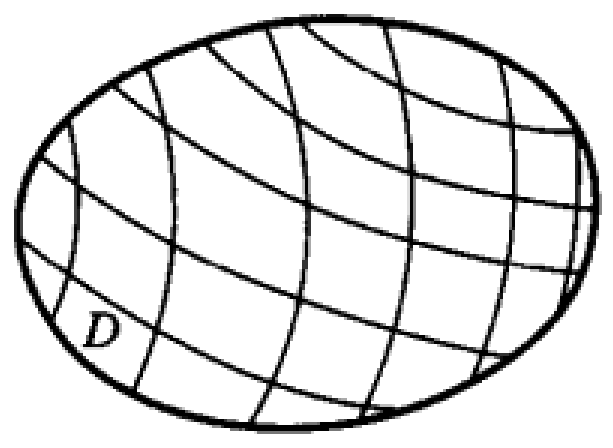
\includegraphics[width=0.32\textwidth]{work/figures/fig20-1}\caption{\relax}\label{fig:20-1}
\end{figure}

为了说清这个问题，我们先考虑平面上的多边形，平面上的多边形是指边界为有限条直线所围成的平面图形，它是有确定的面积的．对于一般的平面图形 $D$，我们自然想到用多边形去逼近它，这种逼近通常有两种，一种是外包的，一种是内含的．称多边形 $P_{1}$ 为 $D$ 的\emph{外包多边形}，如果对任意 $x\in D$，都有 $x\in P_{1}$；称多边形 $P_{2}$ 为 $D$ 的\emph{内含多边形}，如果对任意 $x\in P_{2}$，都有 $x\in D$（见图~\ref{fig:20-2}），这时 $P_{1}$，$P_{2}$ 都有面积，分别记为 $\left|P_{1}\right|$，$\left|P_{2}\right|$．显然，$D$ 要有面积，它必须是所有外包多边形面积的下确界
\[
\inf\left\{\,\left|P_{1}\right|\;\middle|\;P_{1}\ \text{为}\ D\ \text{的外包多边形}\,\right\},
\]
\begin{figure}[htbp]
\centering
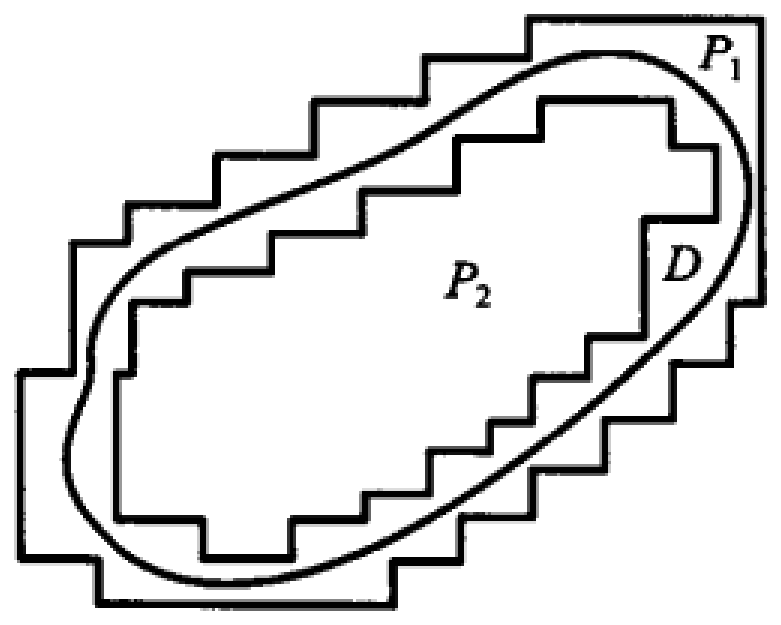
\includegraphics[width=0.34\textwidth]{work/figures/fig20-2}\caption{\relax}\label{fig:20-2}
\end{figure}
同时它也必须是所有内含多边形面积的上确界
\[
\sup\left\{\,\left|P_{2}\right|\;\middle|\;P_{2}\ \text{为}\ D\ \text{的内含多边形}\,\right\}.
\]
因此，$D$ 有面积当且仅当上述下确界等于上确界，即
\[
\inf\left\{\,\left|P_{1}\right|\;\middle|\;P_{1}\ \text{为}\ D\ \text{的外包多边形}\,\right\}
=\sup\left\{\,\left|P_{2}\right|\;\middle|\;P_{2}\ \text{为}\ D\ \text{的内含多边形}\,\right\},
\]
而且面积就等于这个上、下确界的公共值．

在定积分应用中，我们曾经介绍过如何求平面图形的面积．在这里需要指出的是，用定积分求出的面积同上述定义的面积是一致的．事实上，设 $f(x)\geqslant 0$ 在 $[a,b]$ 可积，则 $\displaystyle\int_{a}^{b}f(x)\,\mathrm{d}x$ 的几何意义是以 $f(x)$ 为顶的曲边梯形的面积．这时，$f(x)$ 的任一达布下和都是 $D$ 的一个内含多边形面积，$f(x)$ 的任一达布上和都是 $D$ 的一个外包多边形的面积．而达布下和的上确界则是 $f(x)$ 在 $[a,b]$ 的下积分 $\underline{I}$，达布上和的下确界是 $f(x)$ 在 $[a,b]$ 的上积分 $\overline{I}$．我们证明过，$f(x)$ 在 $[a,b]$ 可积，当且仅当上积分等于下积分：$\overline{I}=\underline{I}$，而且这公共值就等于 $f(x)$ 在 $[a,b]$ 的积分值．可见，这两个前后讲的面积概念实质上是一致的．

在定积分应用中，我们计算过用参数方程给出的曲线所包围的图形的面积．因此，我们知道，由逐段光滑曲线围成的平面图形是有面积的．

是否存在没有面积的平面图形呢？当然有，不可积函数的曲线构成的曲边梯形必然是没有面积的．例如，狄利克雷函数
\[
D(x)=\begin{cases}
1, & x\ \text{为有理数},\\
0, & x\ \text{为无理数},
\end{cases}
\]
则以它为顶的在 $[0,1]$ 上的曲边梯形
\[
D=\left\{(x,y)\mid 0\leqslant x\leqslant 1,0\leqslant y\leqslant D(x)\right\}
\]
就是没有面积的，因为它的外包多边形面积的下确界为 $1$，而内含多边形面积的上确界为 $0$．显然，$D$ 不是用逐段光滑曲线围成的平面图形．

在下面讨论二重积分时，总假定 $D$ 用逐段光滑曲线围成，因而是有面积的．

很容易把上述可求面积的概念推广到三维空间，建立可求体积的空间图形的概念．类似的讨论推广到一般的 $n$ 维空间也就没有任何困难了．

第二，什么叫 $D$ 的分法越来越细？对应于一维的 $\lambda=\max\limits_{1\leqslant i\leqslant n}\left\{\Delta x_{i}\right\}\to 0$，自然会认为可取 $\Delta\sigma_{i}$ 面积的最大者趋向于 $0$，但这实际上是不正确的．因为平面上一个图形 $\Delta\sigma_{i}$，无论它的面积多么小，都可能有其上的两点，它们的距离很大．这样，在求薄板质量的问题中，$f(\xi_{i},\eta_{i})\Delta\sigma_{i}$ 未必是 $\Delta\sigma_{i}$ 质量的近似值．为了保证 $\Delta\sigma_{i}$ 中任意两点的距离任意小，我们引入平面集合 $\bm{S}$ 的\emph{直径}的概念，称 $\bm{S}$ 中所有两点间的距离的上确界为 $\bm{S}$ 的直径，记为 $d(\bm{S})$，即
\[
d(\bm{S})=\sup\left\{r(P_{1},P_{2})\mid P_{1}\in\bm{S},P_{2}\in\bm{S}\right\},
\]
其中 $r(P_{1},P_{2})$ 表示 $P_{1}$ 与 $P_{2}$ 两点间的距离．有了集合直径的概念后，便可以令
\[
d=\max\left(d_{1},d_{2},\cdots,d_{n}\right),
\]
其中 $d_{i}=d(\Delta\sigma_{i})$ 是 $\Delta\sigma_{i}$ 的直径，则 $d\to 0$ 便描述了 $D$ 的分法越来越细，而这些显然都可以完全一样地推广到三维空间．

现在我们可以叙述二重积分的定义了．

\begin{definition}\label{def:20-1}
设 $D$ 是平面上可求面积的有界闭区域，$f(x,y)$ 定义在 $D$ 上，用任意曲线网将 $D$ 分成有限个可求面积的区域 $\Delta\sigma_{1},\Delta\sigma_{2},\cdots,\Delta\sigma_{n}$（称为 $D$ 的一个\emph{分法}），任取 $(\xi_{i},\eta_{i})\in\Delta\sigma_{i}$，$\Delta\sigma_{i}$ 既表示小块平面区域，也表示这小块区域的面积．作和
\[
\sigma=\sum_{i=1}^{n}f(\xi_{i},\eta_{i})\Delta\sigma_{i}.
\]
记 $d_{i}$ 为 $\Delta\sigma_{i}$ 的直径，$\lambda=\max\limits_{1\leqslant i\leqslant n}\left\{d_{i}\right\}$．如果当 $\lambda\to 0$ 时，$\sigma$ 的极限存在，则称 $f(x,y)$ 在 $D$ \emph{可积}，并称极限值为 $f(x,y)$ 在 $D$ 的\emph{二重积分}，记为
\[
\iint\limits_{D}f(P)\,\mathrm{d}\sigma\quad\text{或}\quad\iint\limits_{D}f(x,y)\,\mathrm{d}x\mathrm{d}y.
\]
也就是说，
\[
\iint_{D}f(x,y)\,\mathrm{d}x\mathrm{d}y=\iint_{D}f(P)\,\mathrm{d}\sigma=\lim_{\lambda\to 0}\sum_{i=1}^{n}f(\xi_{i},\eta_{i})\Delta\sigma_{i}.
\]
\end{definition}

和一元定积分的符号相类似，符号 $\displaystyle\iint_{D}f(P)\,\mathrm{d}\sigma$ 表示函数 $f(P)$ 与平面面积微元 $\mathrm{d}\sigma$ 乘积的``连续和''．而符号 $\displaystyle\iint_{D}f(x,y)\,\mathrm{d}x\mathrm{d}y$ 则侧重指出函数的积分变量是 $x$ 与 $y$，但也同时表示函数 $f(x,y)$ 与用平行于坐标轴的直线来作区域分法时的面积微元 $\mathrm{d}x\,\mathrm{d}y$ 的乘积之``连续和''（见图~\ref{fig:20-3}），以后将看到，与定积分不同的是，在变量代换时，他们不能看作 $x$，$y$ 微分的乘积．

\begin{figure}[htbp]
\centering
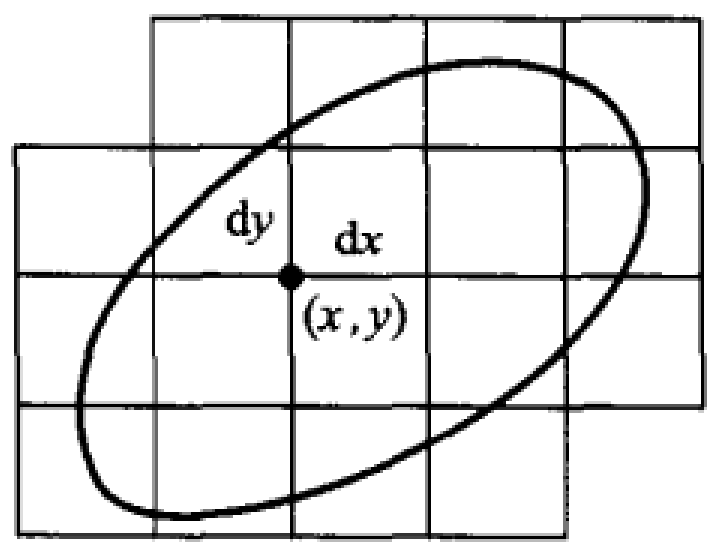
\includegraphics[width=0.32\textwidth]{work/figures/fig20-3}\caption{\relax}\label{fig:20-3}
\end{figure}

另外，值得说明的是，$\lambda$ 是依赖于 $D$ 的分法的．而和式 $\sigma$ 不仅依赖于 $D$ 的分法，而且还依赖于 $(\xi_{i},\eta_{i})\in\Delta\sigma_{i}$ 的取法．因此，所谓和式 $\sigma$ 的极限，严格地说应该用 $\varepsilon$-$\delta$ 语言来刻画．也就是说，若存在某定数 $I$，对任意给定的 $\varepsilon>0$，存在 $\delta>0$，使得对 $D$ 的任意分法 $T=\left\{\Delta\sigma_{i}\mid i=1,2,\cdots,n\right\}$，任意 $(\xi_{i},\eta_{i})\in\Delta\sigma_{i}$，只要 $\lambda=\max\limits_{1\leqslant i\leqslant n}\left\{d(\Delta\sigma_{i})\right\}<\delta$，就有
\[
\left|\sum_{i=1}^{n}f(\xi_{i},\eta_{i})\Delta\sigma_{i}-I\right|<\varepsilon,
\]
则称 $I$ 为函数 $f(x,y)$ 在 $D$ 的二重积分，记为
\[
I=\iint\limits_{D}f(x,y)\,\mathrm{d}x\mathrm{d}y.
\]

下面给出二重积分的几何解释．为简单起见，设 $D=[a,b]\times[c,d]$ 是一矩形区域，$f(x,y)\geqslant 0$ 在 $D$ 连续．这时，$z=f(x,y)$ 表示一曲面，而以 $D$ 为底，以曲面 $z=f(x,y)$ 为顶便构成一曲顶柱体．对于 $D$ 的任意分法（例如由平行于坐标轴的直线网给出）$\Delta\sigma_{i}$，$i=1,2,\cdots,n$，以及任取的 $(\xi_{i},\eta_{i})\in\Delta\sigma_{i}$，$f(\xi_{i},\eta_{i})\Delta\sigma_{i}$ 表示以 $\Delta\sigma_{i}$ 为底、以 $f(\xi_{i},\eta_{i})$ 为高的平顶柱体的体积，它是以 $\Delta\sigma_{i}$ 为底，以 $z=f(x,y)$ 为顶的曲顶柱体体积的近似，因此
\[
\sigma=\sum_{i=1}^{n}f(\xi_{i},\eta_{i})\Delta\sigma_{i}
\]
是整个 $D$ 上曲顶柱体体积的近似．当 $\lambda\to 0$ 时，这个和的极限便是 $D$ 上曲顶柱体的体积，而它也同时是 $f(x,y)$ 在 $D$ 的二重积分．故
\[
\iint_{D}f(x,y)\,\mathrm{d}x\mathrm{d}y=\lim_{\lambda\to 0}\sum_{i=1}^{n}f(\xi_{i},\eta_{i})\Delta\sigma_{i}
\]
的几何意义便是以 $D$ 为底，以 $z=f(x,y)$ 为顶的曲顶柱体的体积（图~\ref{fig:20-4}）．

\begin{figure}[htbp]
\centering
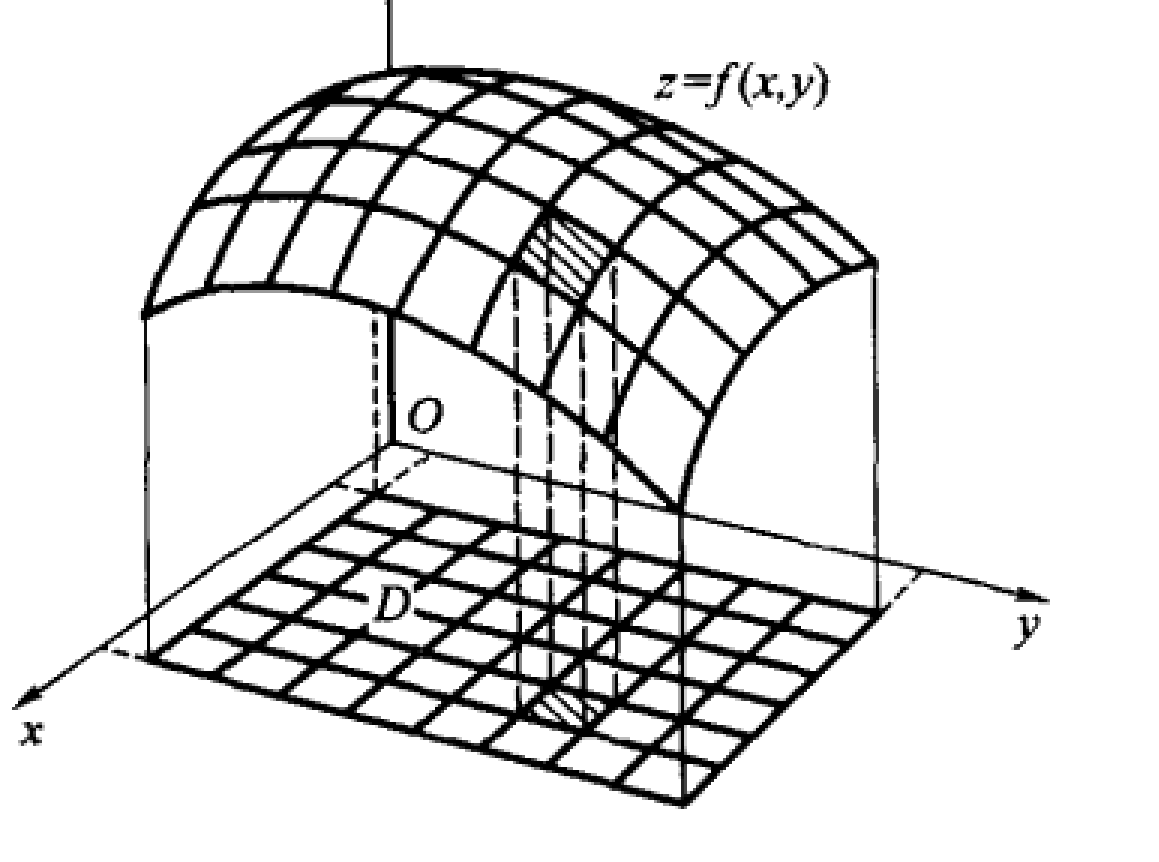
\includegraphics[width=0.42\textwidth]{work/figures/fig20-4}\caption{\relax}\label{fig:20-4}
\end{figure}

当 $D$ 不是矩形而是一般的区域时，$f(x,y)$ 在 $D$ 上的积分的几何解释仍然是以 $D$ 为底，以 $z=f(x,y)$ 为顶，由过 $D$ 的边界平行于 $z$ 轴的直线围成的曲顶柱体的体积，当然这时要假定 $f(x,y)\geqslant 0$（图~\ref{fig:20-5}）．

\begin{figure}[htbp]
\centering
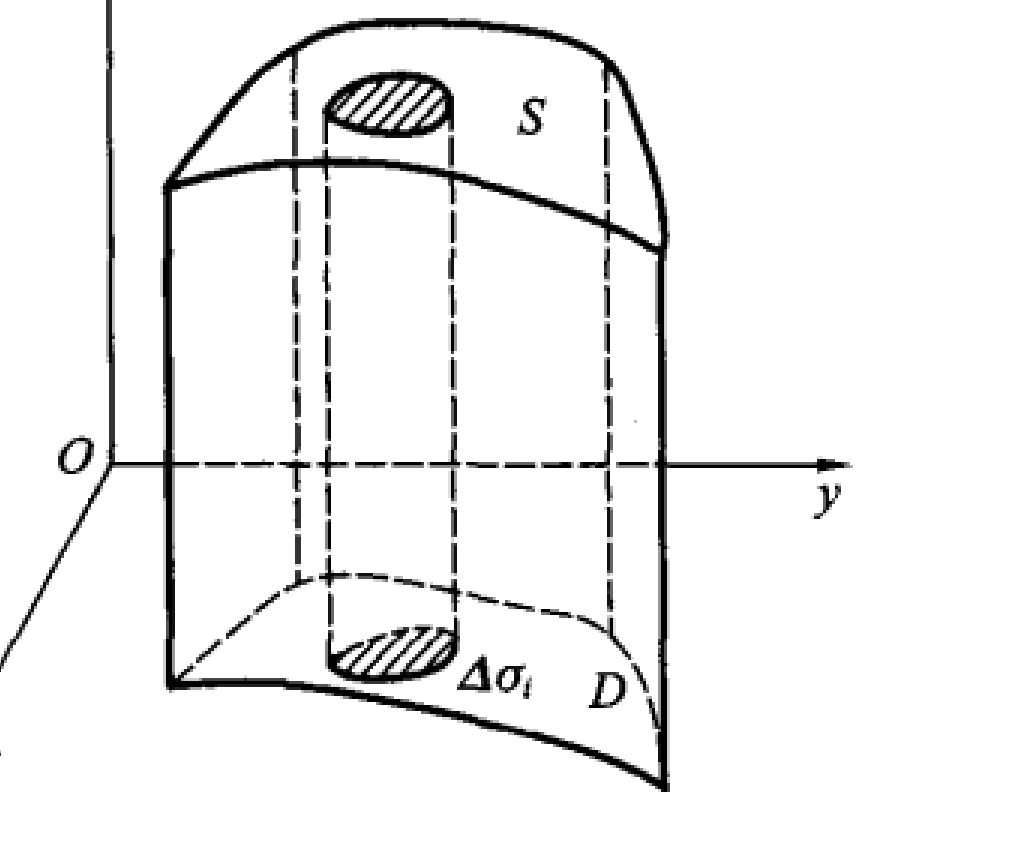
\includegraphics[width=0.40\textwidth]{work/figures/fig20-5}\caption{\relax}\label{fig:20-5}
\end{figure}

当 $f(x,y)$ 可正可负时，积分是相应的曲顶或曲底柱体的体积的代数和，这和一元函数定积分的情形是类似的．

可以完全仿照一元定积分建立二重积分的可积性理论．由此可以证明，逐段光滑曲线围成的有界闭区域 $D$ 上的连续函数在 $D$ 是可积的．还可进一步证明，若 $f$ 是有界闭区域 $D$ 上的有界函数，它只在 $D$ 内的有限段光滑曲线上间断，而在 $D$ 的其余地方均连续，则 $f$ 在 $D$ 可积．

不难由定义和可积性理论证明下面的二重积分基本性质．我们把证明留给读者作为习题．

\begin{ziti}
\item 若 $f(P)$ 在 $D$ 可积，$k$ 为常数，则 $kf(P)$ 也在 $D$ 可积，且
\[
\iint_{D}kf(P)\,\mathrm{d}\sigma=k\iint_{D}f(P)\,\mathrm{d}\sigma.
\]
\item 若 $f(P)$，$g(P)$ 都在 $D$ 可积，则 $f(P)\pm g(P)$，$f(P)g(P)$ 也在 $D$ 可积，并且
\[
\iint_{D}\left[f(P)\pm g(P)\right]\mathrm{d}\sigma=\iint_{D}f(P)\,\mathrm{d}\sigma\pm\iint_{D}g(P)\,\mathrm{d}\sigma.
\]
\item （可加性）若 $D$ 由 $D_{1}$，$D_{2}$ 组成：$D=D_{1}\cup D_{2}$，且 $D_{1}$，$D_{2}$ 除边界外不相交，则 $f(P)$ 在 $D$ 可积的充要条件是 $f(P)$ 在 $D_{1}$，$D_{2}$ 均可积，且
\[
\iint_{D}f(P)\,\mathrm{d}\sigma=\iint_{D_{1}}f(P)\,\mathrm{d}\sigma+\iint_{D_{2}}f(P)\,\mathrm{d}\sigma.
\]
\item （单调性）若 $f$ 与 $g$ 都在 $D$ 可积，且在 $D$ 的每点 $P$ 都有 $f(P)\leqslant g(P)$，则
\[
\iint_{D}f(P)\,\mathrm{d}\sigma\leqslant\iint_{D}g(P)\,\mathrm{d}\sigma.
\]
\item 若 $f(P)$ 在 $D$ 可积，则 $\left|f(P)\right|$ 也在 $D$ 可积，并且
\[
\left|\iint\limits_{D}f(P)\,\mathrm{d}\sigma\right|\leqslant\iint\limits_{D}\left|f(P)\right|\mathrm{d}\sigma.
\]
\item （积分中值定理）设 $D$ 是有界闭区域（因而是连通的），$f(P)$ 在 $D$ 上连续，则存在 $P_{0}\in D$，使得
\[
\iint_{D}f(P)\,\mathrm{d}\sigma=f(P_{0})\left|D\right|,
\]
其中 $\left|D\right|$ 表示 $D$ 的面积．
\end{ziti}

很容易把上述讨论推广到高维，建议读者写出三重积分
\[
\iiint\limits_{V}f(P)\,\mathrm{d}V\quad\text{或}\quad\iiint\limits_{V}f(x,y,z)\,\mathrm{d}x\mathrm{d}y\mathrm{d}z
\]
的定义，其中 $V$ 是三维空间中可求体积的有界闭区域．由于四维空间无法用图形画出来，故三重积分的几何解释——四维空间曲顶柱体的体积，就不如二重积分那么直观了．

\begin{xiti}
\item 证明性质（4），性质（6）．
\item 证明有界闭区域上的连续函数必可积．
\item 设 $\Omega$ 是可度量的平面图形或空间立体，$f$，$g$ 在 $\Omega$ 上连续，证明：
\begin{ziti}
\item 若在 $\Omega$ 上 $f(P)\geqslant 0$，且 $f(P)\not\equiv 0$，则 $\displaystyle\int_{\Omega}f(P)\,\mathrm{d}\Omega>0$；
\item 若在 $\Omega$ 的任何部分区域 $\Omega'\subset\Omega$ 上，有
\[
\int_{\Omega'}f(P)\,\mathrm{d}\Omega=\int_{\Omega'}g(P)\,\mathrm{d}\Omega,
\]
则在 $\Omega$ 上有 $f(P)\equiv g(P)$．
\end{ziti}
\item 设 $f(x)$ 在 $[a,b]$ 可积，$g(y)$ 在 $[c,d]$ 可积，则 $f(x)g(y)$ 在矩形区域 $D=[a,b]\times[c,d]$ 上可积，且
\[
\iint_{D}f(x)g(y)\,\mathrm{d}x\mathrm{d}y=\int_{a}^{b}f(x)\,\mathrm{d}x\int_{c}^{d}g(y)\,\mathrm{d}y.
\]
\item 若 $\left|f(x,y)\right|$ 在 $D$ 上可积，那么 $f(x,y)$ 在 $D$ 上是否可积？考察函数
\[
f(x,y)=\begin{cases}
1, & \text{若}\ x,y\ \text{都是有理数},\\
-1, & \text{若}\ x,y\ \text{至少有一个是无理数}
\end{cases}
\]
在 $[0,1]\times[0,1]$ 上的积分．
\item 设 $D=[0,1]\times[0,1]$，
\[
f(x,y)=\begin{cases}
1, & x\ \text{是有理数},\\
0, & x\ \text{是无理数},
\end{cases}
\]
证明 $f(x,y)$ 在 $D$ 上不可积．
\end{xiti}

\section{重积分化累次积分}\label{sec:20-2}

\subsection{二重积分化累次积分}

我们已经知道二重积分的几何解释是以 $z=f(x,y)$ 为顶，以 $D$ 为底的曲顶柱体的体积．先看 $D$ 为矩形 $[a,b]\times[c,d]$ 的情形．在含参变量积分的讨论中，我们已知 $\displaystyle\int_{c}^{d}f(x_{0},y)\,\mathrm{d}y$ 的几何意义是用垂直于 $x$ 轴的平面 $x=x_{0}$ 去截曲顶柱体，得一曲边梯形，曲顶为 $z=f(x_{0},y)$，$c\leqslant y\leqslant d$．该曲边梯形的面积便是
\[
A(x_{0})=\int_{c}^{d}f(x_{0},y)\,\mathrm{d}y.
\]
由 $x_{0}\in[a,b]$ 的任意性，知曲顶柱体的平行截面面积为 $A(x)$ $(a\leqslant x\leqslant b)$，因此它的体积是
\[
\iint_{D}f(x,y)\,\mathrm{d}x\mathrm{d}y=\int_{a}^{b}A(x)\,\mathrm{d}x=\int_{a}^{b}\mathrm{d}x\int_{c}^{d}f(x,y)\,\mathrm{d}y.
\]
类似地可以得到
\[
\iint_{D}f(x,y)\,\mathrm{d}x\mathrm{d}y=\int_{c}^{d}\mathrm{d}y\int_{a}^{b}f(x,y)\,\mathrm{d}x.
\]
一般地我们有下述定理．

\begin{theorem}\label{thm:20-1}
若 $f(x,y)$ 在矩形区域 $D=[a,b]\times[c,d]$ 上可积，并且对 $[a,b]$ 上的任何 $x$，含参变量积分
\[
A(x)=\int_{c}^{d}f(x,y)\,\mathrm{d}y
\]
存在，则
\[
\iint_{D}f(x,y)\,\mathrm{d}x\mathrm{d}y=\int_{a}^{b}\mathrm{d}x\int_{c}^{d}f(x,y)\,\mathrm{d}y.
\]
\end{theorem}

\begin{proof}
用平行于坐标轴的直线网
\[
a=x_{0}<x_{1}<\cdots<x_{n}=b,\qquad c=y_{0}<y_{1}<\cdots<y_{m}=d
\]
将 $D$ 分为若干个小矩形 $\Delta\sigma_{ij}=[x_{i-1},x_{i}]\times[y_{j-1},y_{j}]$．记 $f(x,y)$ 在 $\Delta\sigma_{ij}$ 的上、下确界分别为 $M_{ij}$ 和 $m_{ij}$．任取 $\xi_{i}\in[x_{i-1},x_{i}]$，则
\[
m_{ij}\Delta y_{j}\leqslant\int_{y_{j-1}}^{y_{j}}f(\xi_{i},y)\,\mathrm{d}y\leqslant M_{ij}\Delta y_{j},\quad i=1,2,\cdots,n,\ j=1,2,\cdots,m.
\]
对 $j$ 求和，得
\[
\sum_{j=1}^{m}m_{ij}\Delta y_{j}\leqslant\int_{c}^{d}f(\xi_{i},y)\,\mathrm{d}y=A(\xi_{i})\leqslant\sum_{j=1}^{m}M_{ij}\Delta y_{j},\quad i=1,2,\cdots,n.
\]
乘以 $\Delta x_{i}$ 后再对 $i$ 求和得
\[
\sum_{i=1}^{n}\sum_{j=1}^{m}m_{ij}\Delta x_{i}\Delta y_{j}\leqslant\sum_{i=1}^{n}A(\xi_{i})\Delta x_{i}\leqslant\sum_{i=1}^{n}\sum_{j=1}^{m}M_{ij}\Delta x_{i}\Delta y_{j}.
\]
当 $\lambda=\max\limits_{\begin{subarray}{c}1\leqslant i\leqslant n\\ 1\leqslant j\leqslant m\end{subarray}}\left\{\Delta\sigma_{ij}\ \text{的直径}\right\}\to 0$ 时，$\lambda'=\max\limits_{1\leqslant i\leqslant n}\left\{\Delta x_{i}\right\}\to 0$．由 $f(x,y)$ 在 $D$ 上可积知，上式左、右两端当 $\lambda\to 0$ 时有公共极限值 $\displaystyle\iint_{D}f(x,y)\,\mathrm{d}x\mathrm{d}y$，因此
\[
\lim_{\lambda'\to 0}\sum_{i=1}^{n}A(\xi_{i})\Delta x_{i}=\iint_{D}f(x,y)\,\mathrm{d}x\mathrm{d}y.
\]
由定积分定义即得
\[
\int_{a}^{b}A(x)\,\mathrm{d}x=\iint_{D}f(x,y)\,\mathrm{d}x\mathrm{d}y.
\]
把 $A(x)$ 的表达式代进去，便得
\[
\iint_{D}f(x,y)\,\mathrm{d}x\mathrm{d}y=\int_{a}^{b}\mathrm{d}x\int_{c}^{d}f(x,y)\,\mathrm{d}y.
\]
定理~\ref{thm:20-1}证完．
\end{proof}

当 $f(x,y)$ 取形式 $f_{1}(x)f_{2}(y)$ 时，定理~\ref{thm:20-1}的结论变成
\[
\iint_{D}f_{1}(x)f_{2}(y)\,\mathrm{d}x\mathrm{d}y=\int_{a}^{b}f_{1}(x)\,\mathrm{d}x\int_{c}^{d}f_{2}(y)\,\mathrm{d}y,
\]
这是§\ref{sec:20-1} 习题 4 曾经要读者证明的．

\begin{corollary}\label{cor:20-2-1}
设 $f(x,y)$ 在 $D=[a,b]\times[c,d]$ 上连续，则
\[
\iint_{D}f(x,y)\,\mathrm{d}x\mathrm{d}y=\int_{a}^{b}\mathrm{d}x\int_{c}^{d}f(x,y)\,\mathrm{d}y=\int_{c}^{d}\mathrm{d}y\int_{a}^{b}f(x,y)\,\mathrm{d}x.
\]
\end{corollary}

\begin{proof}
$f(x,y)$ 在 $D$ 上连续故可积，而且含参变量积分
\[
\int_{c}^{d}f(x,y)\,\mathrm{d}y\quad\text{和}\quad\int_{a}^{b}f(x,y)\,\mathrm{d}x
\]
都存在，由定理~\ref{thm:20-1}立得结论成立．
\end{proof}

定理~\ref{thm:20-1} 告诉我们在定理的条件下，二重积分可以化为累次积分来计算．而推论~\ref{cor:20-2-1} 告诉我们，当 $f$ 连续时，两个累次积分可以任意交换次序，或说累次积分与次序无关．

定理~\ref{thm:20-1}和推论~\ref{cor:20-2-1}揭示了重积分与累次积分的联系，二重积分的两个符号中，$\displaystyle\iint_{D}f(x,y)\,\mathrm{d}x\mathrm{d}y$ 较 $\displaystyle\iint_{D}f(P)\,\mathrm{d}\sigma$ 更好地反映出这一点．

\begin{example}\label{ex:20-2-1}
计算 $\displaystyle\iint_{D}x(x-y)^{2}\,\mathrm{d}x\mathrm{d}y$，其中 $D=[0,1]\times[0,1]$．
\end{example}

\begin{proof}[解]
\[
\begin{aligned}
\iint_{D}x(x-y)^{2}\,\mathrm{d}x\mathrm{d}y&=\int_{0}^{1}x\,\mathrm{d}x\int_{0}^{1}(x-y)^{2}\,\mathrm{d}y\\
&=\int_{0}^{1}-\frac{1}{3}x(x-y)^{3}\bigg|_{0}^{1}\,\mathrm{d}x=\frac{1}{3}\int_{0}^{1}x\left[x^{3}-(x-1)^{3}\right]\mathrm{d}x\\
&=\frac{1}{3}\int_{0}^{1}x(3x^{2}-3x+1)\,\mathrm{d}x=\frac{1}{3}\left[\frac{3}{4}x^{4}-x^{3}+\frac{1}{2}x^{2}\right]\bigg|_{0}^{1}\\
&=\frac{1}{12}.
\end{aligned}
\]
\end{proof}

下面要把定理~\ref{thm:20-1} 的矩形区域推广到一般的非矩形区域．我们先讨论简单区域．所谓\emph{简单区域} $D$ 是指区域的边界与平行于某一坐标轴（$x$ 轴或 $y$ 轴）的直线相交至多两点，或有部分边界是平行于坐标轴的．如图~\ref{fig:20-6} 和图~\ref{fig:20-7} 所示．对于简单区域 $D$，它至少可表为下列情形之一
\begin{equation}\label{eq:20-2-1}
D=\left\{(x,y)\mid y_{1}(x)\leqslant y\leqslant y_{2}(x),a\leqslant x\leqslant b\right\},
\tag{1}
\end{equation}
\begin{equation}\label{eq:20-2-2}
D=\left\{(x,y)\mid x_{1}(y)\leqslant x\leqslant x_{2}(y),c\leqslant y\leqslant d\right\}.
\tag{2}
\end{equation}

\begin{figure}[htbp]
\centering
\begin{tikzpicture}[scale=0.85,baseline=(current bounding box.center)]
  \fill[gray!12] (0.6,0.3) .. controls (1.2,1.6) and (2.6,1.9) .. (3.3,1.2)
    .. controls (3.6,0.5) and (2.6,0.1) .. (1.6,0.15) .. controls (1.0,0.18) .. (0.6,0.3);
  \draw[{-Latex}] (0,0) -- (4.2,0) node[below left] {$x$};
  \draw[{-Latex}] (0,0) -- (0,2.3) node[below left] {$y$};
  \draw (0.6,0.3) .. controls (1.2,1.6) and (2.6,1.9) .. (3.3,1.2);
  \draw (3.3,1.2) .. controls (3.6,0.5) and (2.6,0.1) .. (1.6,0.15) .. controls (1.0,0.18) .. (0.6,0.3);
  \draw[dashed] (1.9,0) -- (1.9,1.62);
  \node at (1.9,1.75) {$y_{2}(x)$};
  \node at (1.75,-0.28) {$y_{1}(x)$};
  \node at (0.55,-0.28) {$a$};
  \node at (3.35,-0.28) {$b$};
  \draw (1.9,0.18) -- (1.9,0.6);
\end{tikzpicture}\caption{\relax}\label{fig:20-6}
\end{figure}

\begin{figure}[htbp]
\centering
\begin{tikzpicture}[scale=0.85,baseline=(current bounding box.center)]
  \fill[gray!12] (0.6,0.3) .. controls (1.2,1.6) and (2.6,1.9) .. (3.3,1.2)
    .. controls (3.6,0.5) and (2.6,0.1) .. (1.6,0.15) .. controls (1.0,0.18) .. (0.6,0.3);
  \draw[{-Latex}] (0,0) -- (4.2,0) node[below left] {$x$};
  \draw[{-Latex}] (0,0) -- (0,2.3) node[below left] {$y$};
  \draw (0.6,0.3) .. controls (1.2,1.6) and (2.6,1.9) .. (3.3,1.2);
  \draw (3.3,1.2) .. controls (3.6,0.5) and (2.6,0.1) .. (1.6,0.15) .. controls (1.0,0.18) .. (0.6,0.3);
  \draw[dashed] (0,1.1) -- (3.45,1.1);
  \node[left] at (0,1.1) {\small $c$};
  \node[right] at (3.55,1.1) {\small $x_{2}(y)$};
  \node[left] at (0.45,1.1) {\small $x_{1}(y)$};
\end{tikzpicture}\caption{\relax}\label{fig:20-7}
\end{figure}

\begin{theorem}\label{thm:20-2}
设 $D$ 由\eqref{eq:20-2-1}式给出，$y_{1}(x)$，$y_{2}(x)$ 在 $[a,b]$ 上连续，$f(x,y)$ 在 $D$ 上连续，则
\[
\iint_{D}f(x,y)\,\mathrm{d}x\mathrm{d}y=\int_{a}^{b}\mathrm{d}x\int_{y_{1}(x)}^{y_{2}(x)}f(x,y)\,\mathrm{d}y.
\]
\end{theorem}

\begin{proof}
$y_{1}(x)$，$y_{2}(x)$ 在 $[a,b]$ 上连续，故 $y_{1}(x)$ 在 $[a,b]$ 上有最小值 $c$，$y_{2}(x)$ 在 $[a,b]$ 有最大值 $d$，故 $D\subset[a,b]\times[c,d]$．构造 $D$ 上的延拓函数 $\tilde{f}$
\[
\tilde{f}(x,y)=\begin{cases}
f(x,y), & (x,y)\in D,\\
0, & (x,y)\notin D.
\end{cases}
\]
由二重积分的性质（3）知 $\tilde{f}$ 在 $[a,b]\times[c,d]$ 可积，且
\[
\begin{aligned}
\iint\limits_{D}f(x,y)\,\mathrm{d}x\mathrm{d}y&=\iint\limits_{[a,b]\times[c,d]}\tilde{f}(x,y)\,\mathrm{d}x\mathrm{d}y
=\int_{a}^{b}\mathrm{d}x\int_{c}^{d}\tilde{f}(x,y)\,\mathrm{d}y\\
&=\int_{a}^{b}\mathrm{d}x\left[\int_{c}^{y_{1}(x)}\tilde{f}(x,y)\,\mathrm{d}y+\int_{y_{1}(x)}^{y_{2}(x)}\tilde{f}(x,y)\,\mathrm{d}y+\int_{y_{2}(x)}^{d}\tilde{f}(x,y)\,\mathrm{d}y\right]\\
&=\int_{a}^{b}\mathrm{d}x\int_{y_{1}(x)}^{y_{2}(x)}f(x,y)\,\mathrm{d}y.
\end{aligned}
\]
定理~\ref{thm:20-2}证完．
\end{proof}

同理，若 $D$ 由\eqref{eq:20-2-2}式给出，$x_{1}(y)$ 和 $x_{2}(y)$ 在 $[c,d]$ 上连续，$f(x,y)$ 在 $D$ 上连续，则
\[
\iint_{D}f(x,y)\,\mathrm{d}x\mathrm{d}y=\int_{c}^{d}\mathrm{d}y\int_{x_{1}(y)}^{x_{2}(y)}f(x,y)\,\mathrm{d}x.
\]
若 $D$ 既能用\eqref{eq:20-2-1}表示又能用\eqref{eq:20-2-2}表示，且 $x_{1}(y)$，$x_{2}(y)$，$y_{1}(x)$，$y_{2}(x)$ 均连续，$f$ 在 $D$ 上连续，则
\[
\iint_{D}f(x,y)\,\mathrm{d}x\mathrm{d}y=\int_{a}^{b}\mathrm{d}x\int_{y_{1}(x)}^{y_{2}(x)}f(x,y)\,\mathrm{d}y=\int_{c}^{d}\mathrm{d}y\int_{x_{1}(y)}^{x_{2}(y)}f(x,y)\,\mathrm{d}x.
\]

从上面二重积分化累次积分的公式可知，如果是先对 $y$ 积分，则 $y$ 的积分限一般是 $x$ 的函数，而最后积分的 $x$ 的积分限只能是常数；同理如果先对 $x$ 积分，则 $x$ 的积分限一般是 $y$ 的函数，而最后积分的 $y$ 的积分限只能是常数．

\begin{example}\label{ex:20-2-2}
求 $\displaystyle\iint_{D}\sqrt{4x^{2}-y^{2}}\,\mathrm{d}x\,\mathrm{d}y$，其中 $D$ 由 $y=0$，$x=1$，$y=x$ 围成．
\end{example}

\begin{proof}[解]
作出 $D$ 的图形．

\begin{figure}[htbp]
\centering
\begin{tikzpicture}[scale=1.15,baseline=(current bounding box.center)]
  \fill[gray!12] (0,0) -- (1,0) -- (1,1) -- cycle;
  \draw[{-Latex}] (-0.3,0) -- (1.6,0) node[below left] {$x$};
  \draw[{-Latex}] (0,-0.3) -- (0,1.6) node[below left] {$y$};
  \draw (0,0) -- (1,1) node[above right] {\small $y=x$};
  \draw (1,0) -- (1,1) node[above right] {\small $x=1$};
  \node at (0.65,0.22) {$D$};
  \node[below] at (1,0) {$1$};
\end{tikzpicture}\caption{\relax}\label{fig:20-8}
\end{figure}

用平行于 $y$ 轴的直线去截 $D$，则对每一 $x\in[0,1]$，有 $0\leqslant y\leqslant x$，故 $D$ 可表示为：$0\leqslant y\leqslant x$，$0\leqslant x\leqslant 1$．因此
\[
\iint_{D}\sqrt{4x^{2}-y^{2}}\,\mathrm{d}x\mathrm{d}y=\int_{0}^{1}\mathrm{d}x\int_{0}^{x}\sqrt{4x^{2}-y^{2}}\,\mathrm{d}y.
\]
对内层定积分作变量代换 $y=2x\sin t$，则
\[
\begin{aligned}
\iint\limits_{D}\sqrt{4x^{2}-y^{2}}\,\mathrm{d}x\mathrm{d}y&=\int_{0}^{1}\mathrm{d}x\int_{0}^{\frac{\pi}{6}}2x\cos t\cdot 2x\cos t\,\mathrm{d}t\\
&=4\int_{0}^{1}x^{2}\,\mathrm{d}x\int_{0}^{\frac{\pi}{6}}\cos^{2}t\,\mathrm{d}t\\
&=\frac{4}{3}x^{3}\bigg|_{0}^{1}\int_{0}^{\frac{\pi}{6}}\frac{1+\cos 2t}{2}\,\mathrm{d}t\\
&=\frac{4}{3}\left[\frac{1}{2}t+\frac{1}{4}\sin 2t\right]\bigg|_{0}^{\frac{\pi}{6}}=\frac{1}{3}\left[\frac{\pi}{3}+\frac{\sqrt{3}}{2}\right].
\end{aligned}
\]
\end{proof}

\begin{example}\label{ex:20-2-3}
求由 $z=xy$，$z=x+y$，$x+y=1$，$x=0$，$y=0$ 围成的区域的体积．
\end{example}

\begin{proof}[解]
空间区域如图~\ref{fig:20-9} 所示，它在 $Oxy$ 面上的投影 $D$ 由 $x+y=1$，$x=0$，$y=0$ 所围成（图~\ref{fig:20-10}）．用平行于 $y$ 轴的直线去截 $D$，则对每一 $x\in[0,1]$，有 $0\leqslant y\leqslant 1-x$．因此 $D$ 可表示为
\[
0\leqslant y\leqslant 1-x,\quad 0\leqslant x\leqslant 1.
\]

\begin{figure}[htbp]
\centering
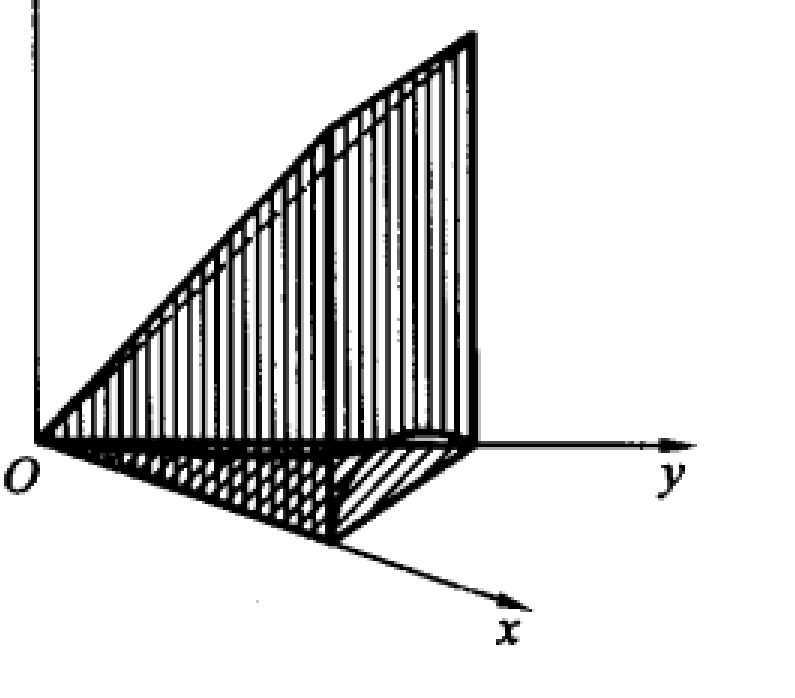
\includegraphics[width=0.34\textwidth]{work/figures/fig20-9}\caption{\relax}\label{fig:20-9}
\end{figure}

\begin{figure}[htbp]
\centering
\begin{tikzpicture}[scale=1.15,baseline=(current bounding box.center)]
  \fill[gray!12] (0,0) -- (1.3,0) -- (0,1.3) -- cycle;
  \draw[{-Latex}] (-0.3,0) -- (1.8,0) node[below left] {$x$};
  \draw[{-Latex}] (0,-0.3) -- (0,1.8) node[below left] {$y$};
  \draw (1.3,0) -- (0,1.3) node[above left] {\small $x+y=1$};
  \node at (0.4,0.35) {$D$};
  \node[below] at (1.3,0) {$1$};
  \node[left] at (0,1.3) {$1$};
\end{tikzpicture}\caption{\relax}\label{fig:20-10}
\end{figure}

故体积 $V$ 为
\[
\begin{aligned}
V&=\iint\limits_{D}\left[(x+y)-xy\right]\mathrm{d}x\mathrm{d}y\\
&=\int_{0}^{1}\mathrm{d}x\int_{0}^{1-x}(x+y-xy)\,\mathrm{d}y\\
&=\int_{0}^{1}\left[xy+\frac{(1-x)}{2}y^{2}\right]\bigg|_{0}^{1-x}\,\mathrm{d}x\\
&=\int_{0}^{1}\left[x(1-x)+\frac{1}{2}(1-x)^{3}\right]\mathrm{d}x\\
&=\left[\frac{1}{2}x^{2}-\frac{1}{3}x^{3}-\frac{1}{8}(1-x)^{4}\right]\bigg|_{0}^{1}=\frac{7}{24}.
\end{aligned}
\]
\end{proof}

\begin{example}\label{ex:20-2-4}
用两种不同的顺序将二重积分
\[
I=\iint\limits_{D}f(x,y)\,\mathrm{d}x\mathrm{d}y
\]
化为累次积分，其中 $D$ 由 $y=0$，$y=x^{3}$，$x+y=2$ 围成．
\end{example}

\begin{proof}[解]
作图．

两曲线 $y=x^{3}$ 和 $x+y=2$ 的交点为 $(1,1)$．

考虑先对 $y$ 积分．用平行于 $y$ 轴的直线去截 $D$，当 $x\in[0,1]$ 时有 $0\leqslant y\leqslant x^{3}$；当 $x\in[1,2]$ 时有 $0\leqslant y\leqslant 2-x$．这样 $D$ 可分为两部分 $D_{1}$ 和 $D_{2}$，其中
\[
\begin{aligned}
&D_{1}:\ 0\leqslant y\leqslant x^{3},\ 0\leqslant x\leqslant 1,\\
&D_{2}:\ 0\leqslant y\leqslant 2-x,\ 1\leqslant x\leqslant 2.
\end{aligned}
\]

\begin{figure}[htbp]
\centering
\begin{tikzpicture}[scale=1.0,baseline=(current bounding box.center)]
  \fill[gray!12] (0,0) plot[smooth,domain=0:1] (\x,\x*\x*\x) -- (2,0) -- cycle;
  \draw[{-Latex}] (-0.3,0) -- (2.5,0) node[below left] {$x$};
  \draw[{-Latex}] (0,-0.3) -- (0,2.5) node[below left] {$y$};
  \draw[smooth,domain=0:1.15] plot (\x,{\x*\x*\x}) node[right] {\small $y=x^{3}$};
  \draw (1,1) -- (2,0) node[below right] {\small $x+y=2$};
  \node at (0.85,0.35) {$D$};
  \node[below] at (1,0) {$1$};
  \node[below] at (2,0) {$2$};
  \node[left] at (0,1) {$1$};
  \draw[dashed] (1,0) -- (1,1);
\end{tikzpicture}\caption{\relax}\label{fig:20-11}
\end{figure}

因此
\[
\begin{aligned}
\iint_{D}f(x,y)\,\mathrm{d}x\mathrm{d}y&=\int_{0}^{1}\mathrm{d}x\int_{0}^{x^{3}}f(x,y)\,\mathrm{d}y+\\
&\quad \int_{1}^{2}\mathrm{d}x\int_{0}^{2-x}f(x,y)\,\mathrm{d}y.
\end{aligned}
\]
再考虑先对 $x$ 积分．用平行于 $x$ 轴的直线去截 $D$，则对每一 $y\in[0,1]$，有 $y^{\frac{1}{3}}\leqslant x\leqslant 2-y$，故 $D$ 又可表为
\[
D:\ y^{\frac{1}{3}}\leqslant x\leqslant 2-y,\ 0\leqslant y\leqslant 1.
\]
因此
\[
\iint_{D}f(x,y)\,\mathrm{d}x\mathrm{d}y=\int_{0}^{1}\mathrm{d}y\int_{y^{\frac{1}{3}}}^{2-y}f(x,y)\,\mathrm{d}x.
\]
\end{proof}

\begin{example}\label{ex:20-2-5}
计算积分
\[
I=\int_{0}^{1}\mathrm{d}x\int_{x}^{\sqrt{x}}\frac{\sin y}{y}\,\mathrm{d}y.
\]
\end{example}

\begin{proof}[解]
这个累次积分是先对 $y$ 积分，再对 $x$ 积分．而 $\dfrac{\sin y}{y}$ 的原函数不能用初等函数表示．因此按上述顺序进行累次积分是行不通的．为此考虑改变积分的顺序．

根据积分限知，将上述积分表为二重积分时，积分区域 $D$ 为 $x\leqslant y\leqslant\sqrt{x}$，$0\leqslant x\leqslant 1$．即 $D$ 由曲线 $y=x$，$y=\sqrt{x}$，$x=0$ 和 $x=1$ 围成．作出 $D$ 的图形如图~\ref{fig:20-12}．用平行于 $x$ 轴的直线去截 $D$，对每一 $y\in[0,1]$，有 $y^{2}\leqslant x\leqslant y$，于是有
\[
\begin{aligned}
I&=\int_{0}^{1}\mathrm{d}x\int_{x}^{\sqrt{x}}\frac{\sin y}{y}\,\mathrm{d}y=\int_{0}^{1}\mathrm{d}y\int_{y^{2}}^{y}\frac{\sin y}{y}\,\mathrm{d}x\\
&=\int_{0}^{1}\frac{\sin y}{y}(y-y^{2})\,\mathrm{d}y=\int_{0}^{1}\sin y\,\mathrm{d}y-\int_{0}^{1}y\sin y\,\mathrm{d}y\\
&=-\cos y\left|_{0}^{1}-(-\cos y+\sin y)\right|_{0}^{1}=1-\sin 1.
\end{aligned}
\]

\begin{figure}[htbp]
\centering
\begin{tikzpicture}[scale=1.3,baseline=(current bounding box.center)]
  \fill[gray!12] (0,0) plot[smooth,domain=0:1] (\x,{sqrt(\x)}) -- (1,1) plot[smooth,domain=1:0] (\x,\x) -- cycle;
  \draw[{-Latex}] (-0.2,0) -- (1.5,0) node[below left] {$x$};
  \draw[{-Latex}] (0,-0.2) -- (0,1.5) node[below left] {$y$};
  \draw[smooth,domain=0:1] plot (\x,{sqrt(\x)}) node[above right] {\small $y=\sqrt{x}$};
  \draw (0,0) -- (1,1) node[below right] {\small $y=x$};
  \node at (0.55,0.6) {$D$};
  \node[below] at (1,0) {$1$};
  \node[left] at (0,1) {$1$};
  \draw[dashed] (1,1) -- (1,0);
  \draw[dashed] (1,1) -- (0,1);
\end{tikzpicture}\caption{\relax}\label{fig:20-12}
\end{figure}

从此例可见，将二重积分化为累次积分时，积分次序对计算是有影响的，选择得不好，可能使计算很繁，甚至积不出来．顺便指出，对上述累次积分除了用改变积分次序的方法进行计算外，还可用分部积分方法进行计算．记
\[
A(x)=\int_{x}^{\sqrt{x}}\frac{\sin y}{y}\,\mathrm{d}y,
\]
则由分部积分得
\[
\begin{aligned}
I&=\int_{0}^{1}A(x)\,\mathrm{d}x=xA(x)\bigg|_{0}^{1}-\int_{0}^{1}xA'(x)\,\mathrm{d}x\\
&=A(1)-\int_{0}^{1}x\left(\frac{\sin\sqrt{x}}{\sqrt{x}}\frac{1}{2\sqrt{x}}-\frac{\sin x}{x}\right)\mathrm{d}x\\
&=-\int_{0}^{1}\frac{1}{2}\sin\sqrt{x}\,\mathrm{d}x+\int_{0}^{1}\sin x\,\mathrm{d}x,
\end{aligned}
\]
在第一项中令 $\sqrt{x}=t$，得
\[
I=-\int_{0}^{1}t\sin t\,\mathrm{d}t+\int_{0}^{1}\sin x\,\mathrm{d}x=1-\sin 1.
\]
\end{proof}

将二重积分化为累次积分，其中最基本的步骤就是根据二重积分的积分域 $D$ 确定累次积分的积分限．这是初学者感到不易掌握和容易出错的地方．作出 $D$ 的图形可以给我们提供非常直观的认识，减少出错率，因此切不可忽视作图．定积分限的方法必须很好地掌握，它是计算重积分最基础的内容．

如果区域 $D$ 能分解成有限个没有公共内点的简单区域的并，则对每个简单区域应用上述积分公式，我们便能计算很多较复杂区域的二重积分．

\subsection{三重积分化累次积分}

对于三重积分
\[
\iiint_{V}f(x,y,z)\,\mathrm{d}x\mathrm{d}y\mathrm{d}z,
\]
其计算也是化为累次积分来计算．下面我们不加证明地给出化累次积分的公式，其中出现的积分都假定是存在的．

（1）$V$ 是长方体 $[a,b]\times[c,d]\times[e,f]$，则有公式
\[
\iiint_{V}f(x,y,z)\,\mathrm{d}x\mathrm{d}y\mathrm{d}z=\int_{a}^{b}\mathrm{d}x\int_{c}^{d}\mathrm{d}y\int_{e}^{f}f(x,y,z)\,\mathrm{d}z.
\]
它完全可以类似于定理~\ref{thm:20-1}一样加以证明．把后面两个累次积分写成重积分，便得
\[
\iiint_{V}f(x,y,z)\,\mathrm{d}x\mathrm{d}y\mathrm{d}z=\int_{a}^{b}\mathrm{d}x\iint_{[c,d]\times[e,f]}f(x,y,z)\,\mathrm{d}y\mathrm{d}z,
\]
这可以看作，对每个固定的 $x$，先对截面积分，然后对 $x$ 按 $a$ 到 $b$ 积分，便得在整个立体 $V$ 的积分．

公式也可以写成
\[
\iiint_{V}f(x,y,z)\,\mathrm{d}x\mathrm{d}y\mathrm{d}z=\iint_{[a,b]\times[c,d]}\mathrm{d}x\mathrm{d}y\int_{e}^{f}f(x,y,z)\,\mathrm{d}z,
\]
这可以看作，在 $[a,b]\times[c,d]$ 中固定的一点 $(x,y)$，先对 $z$ 从 $e$ 到 $f$ 积分，然后再对 $(x,y)$ 在整个 $[a,b]\times[c,d]$ 积分，便得在整个立体 $V$ 的积分．

\begin{figure}[htbp]
\centering
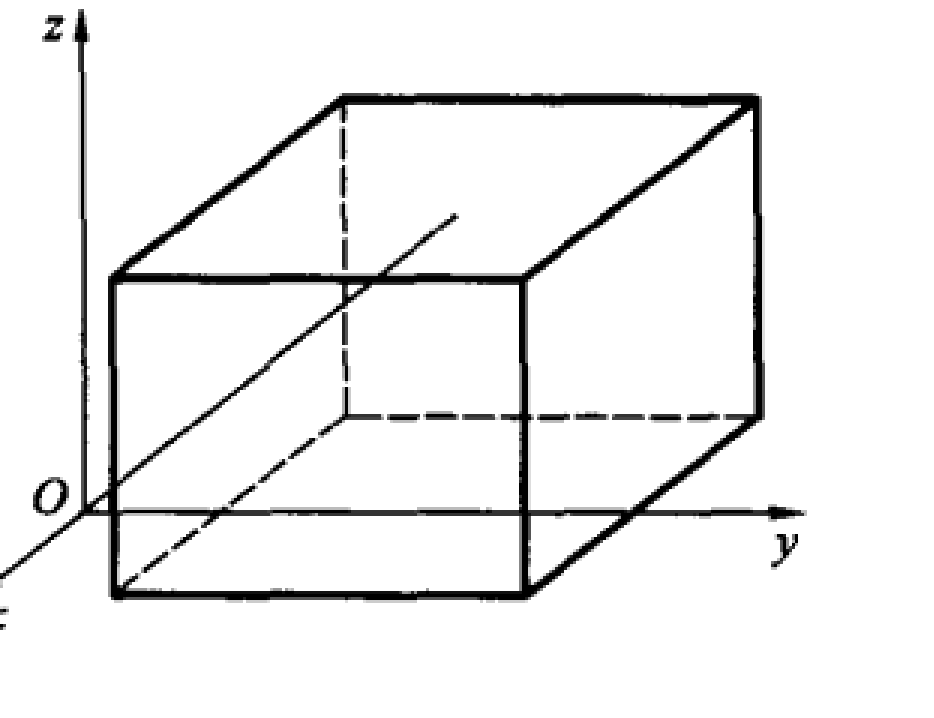
\includegraphics[width=0.32\textwidth]{work/figures/fig20-13}\caption{\relax}\label{fig:20-13}
\end{figure}

（2）设空间立体界于平面 $z=e$ 和 $z=f$ 之间，对每一 $z\in[e,f]$，用平行于 $Oxy$ 面的平面 $z=z$ 去截立体 $V$ 得一平面图形 $D_{z}$（见图~\ref{fig:20-14}），则有
\[
\iiint_{V}f(x,y,z)\,\mathrm{d}x\mathrm{d}y\mathrm{d}z=\int_{e}^{f}\mathrm{d}z\iint_{D_{z}}f(x,y,z)\,\mathrm{d}x\mathrm{d}y.
\]
其中 $\displaystyle\iint_{D_{z}}f(x,y,z)\,\mathrm{d}x\,\mathrm{d}y$ 是展布在平面图形 $D_{z}$ 上的二重积分，$z$ 相对固定不变．一般来说当 $z$ 在 $[e,f]$ 上变动时，所得到的平面图形 $D_{z}$ 是不同的，即 $D_{z}$ 是依赖于 $z$ 的．若 $D_{z}$ 可表示为 $x_{1}(y,z)\leqslant x\leqslant x_{2}(y,z)$，$y_{1}(z)\leqslant y\leqslant y_{2}(z)$（见图~\ref{fig:20-15}），则
\[
\begin{aligned}
\iiint_{V}f(x,y,z)\,\mathrm{d}x\mathrm{d}y\mathrm{d}z&=\int_{e}^{f}\mathrm{d}z\iint_{D_{z}}f(x,y,z)\,\mathrm{d}x\mathrm{d}y\\
&=\int_{e}^{f}\mathrm{d}z\int_{y_{1}(z)}^{y_{2}(z)}\mathrm{d}y\int_{x_{1}(y,z)}^{x_{2}(y,z)}f(x,y,z)\,\mathrm{d}x.
\end{aligned}
\]

\begin{figure}[htbp]
\centering
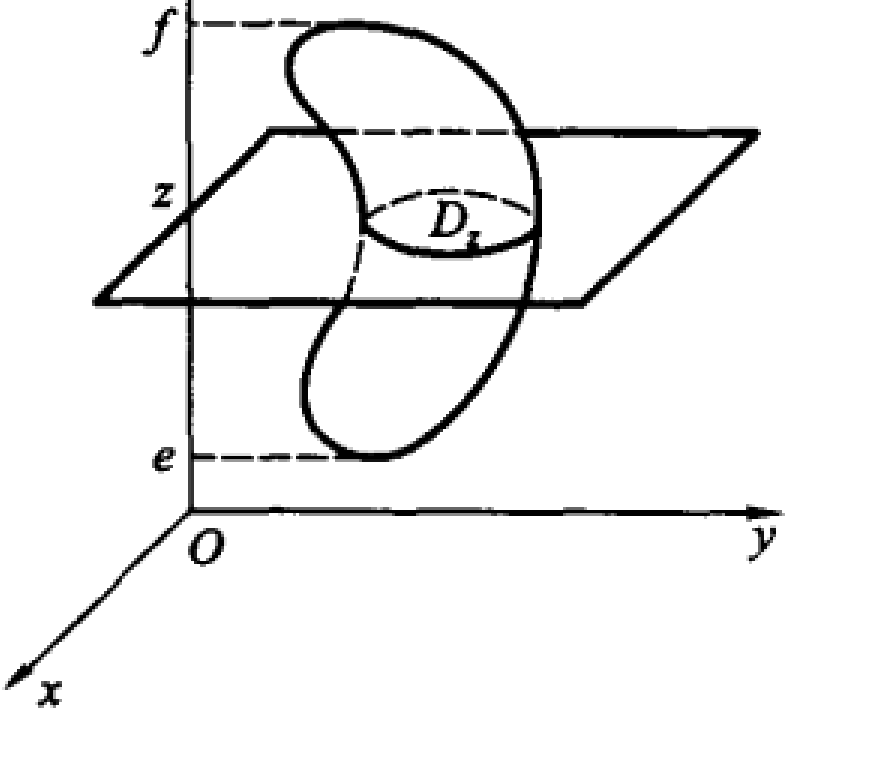
\includegraphics[width=0.32\textwidth]{work/figures/fig20-14}\caption{\relax}\label{fig:20-14}
\end{figure}

\begin{figure}[htbp]
\centering
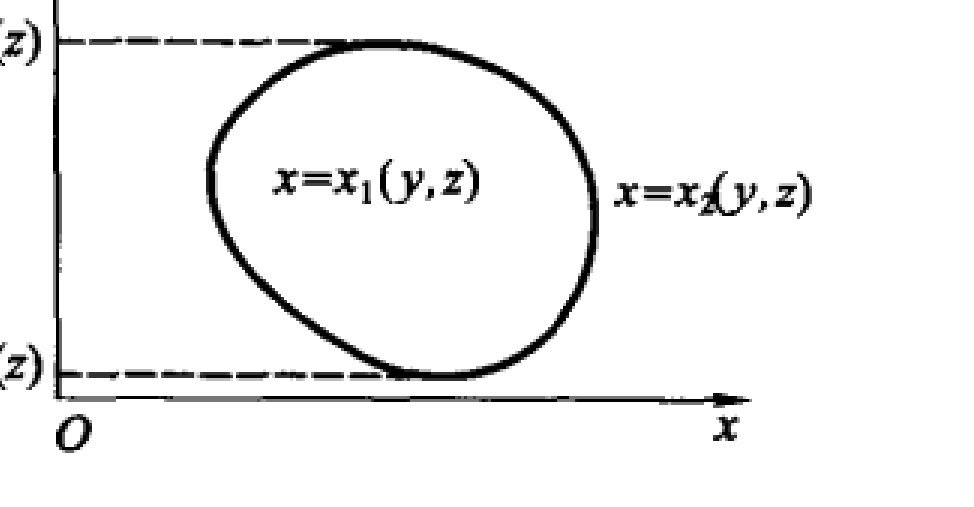
\includegraphics[width=0.34\textwidth]{work/figures/fig20-15}\caption{\relax}\label{fig:20-15}
\end{figure}

通常，先积分者，其积分限是后积分变量的函数，而最后积分者，其积分限只能是常数．

（3）设空间立体 $V$ 在 $Oxy$ 面上的投影 $D$ 是平面上的简单区域．平行于 $z$ 轴且通过 $D$ 的内点的直线与 $V$ 的边界相交至多两点（图~\ref{fig:20-16}）．记下面一点所在的边界曲面为 $z_{1}(x,y)$，上面一点所在的边界曲面为 $z_{2}(x,y)$，则有公式
\[
\iiint_{V}f(x,y,z)\,\mathrm{d}x\mathrm{d}y\mathrm{d}z=\iint_{D}\mathrm{d}x\mathrm{d}y\int_{z_{1}(x,y)}^{z_{2}(x,y)}f(x,y,z)\,\mathrm{d}z.
\]

\begin{figure}[htbp]
\centering
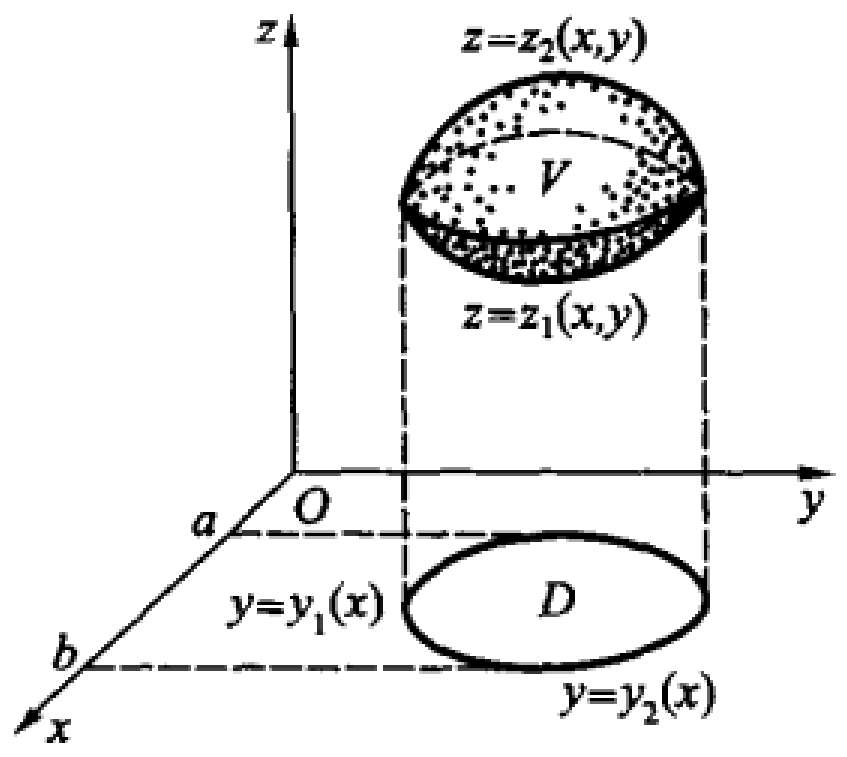
\includegraphics[width=0.32\textwidth]{work/figures/fig20-16}\caption{\relax}\label{fig:20-16}
\end{figure}

又若 $D$ 可表为 $y_{1}(x)\leqslant y\leqslant y_{2}(x)$，$a\leqslant x\leqslant b$，则有
\[
\iiint_{V}f(x,y,z)\,\mathrm{d}x\mathrm{d}y\mathrm{d}z=\int_{a}^{b}\mathrm{d}x\int_{y_{1}(x)}^{y_{2}(x)}\mathrm{d}y\int_{z_{1}(x,y)}^{z_{2}(x,y)}f(x,y,z)\,\mathrm{d}z.
\]

\begin{example}\label{ex:20-2-6}
计算
\[
I=\iiint_{V}\frac{\mathrm{d}x\mathrm{d}y\mathrm{d}z}{(1+x+y+z)^{3}},
\]
其中 $V$ 由 $x=0$，$y=0$，$z=0$，$x+y+z=1$ 围成．
\end{example}

\begin{proof}[解]
区域 $V$ 如图~\ref{fig:20-17}，$V$ 在 $Oxy$ 平面的投影由 $x=0$，$y=0$，$x+y=1$ 围成，这时区域 $V$ 的底为 $z=0$，顶为 $z=1-x-y$．因此
\[
\begin{aligned}
I&=\iint_{D}\mathrm{d}x\mathrm{d}y\int_{0}^{1-x-y}\frac{\mathrm{d}z}{(1+x+y+z)^{3}}\\
&=\int_{0}^{1}\mathrm{d}x\int_{0}^{1-x}\mathrm{d}y\int_{0}^{1-x-y}\frac{\mathrm{d}z}{(1+x+y+z)^{3}}\\
&=\int_{0}^{1}\mathrm{d}x\int_{0}^{1-x}\frac{-1}{2(1+x+y+z)^{2}}\bigg|_{0}^{1-x-y}\,\mathrm{d}y\\
&=\int_{0}^{1}\mathrm{d}x\int_{0}^{1-x}\frac{1}{2}\left[\frac{1}{(1+x+y)^{2}}-\frac{1}{4}\right]\mathrm{d}y\\
&=\frac{1}{2}\int_{0}^{1}\left[-\frac{1}{(1+x+y)}-\frac{y}{4}\right]\bigg|_{0}^{1-x}\,\mathrm{d}x\\
&=\frac{1}{2}\int_{0}^{1}\left(\frac{1}{x+1}-\frac{3-x}{4}\right)\mathrm{d}x\\
&=\frac{1}{2}\left[\ln(1+x)\big|_{0}^{1}+\frac{(3-x)^{2}}{8}\bigg|_{0}^{1}\right]=\frac{1}{2}\left(\ln 2-\frac{5}{8}\right).
\end{aligned}
\]
\end{proof}

\begin{figure}[htbp]
\centering
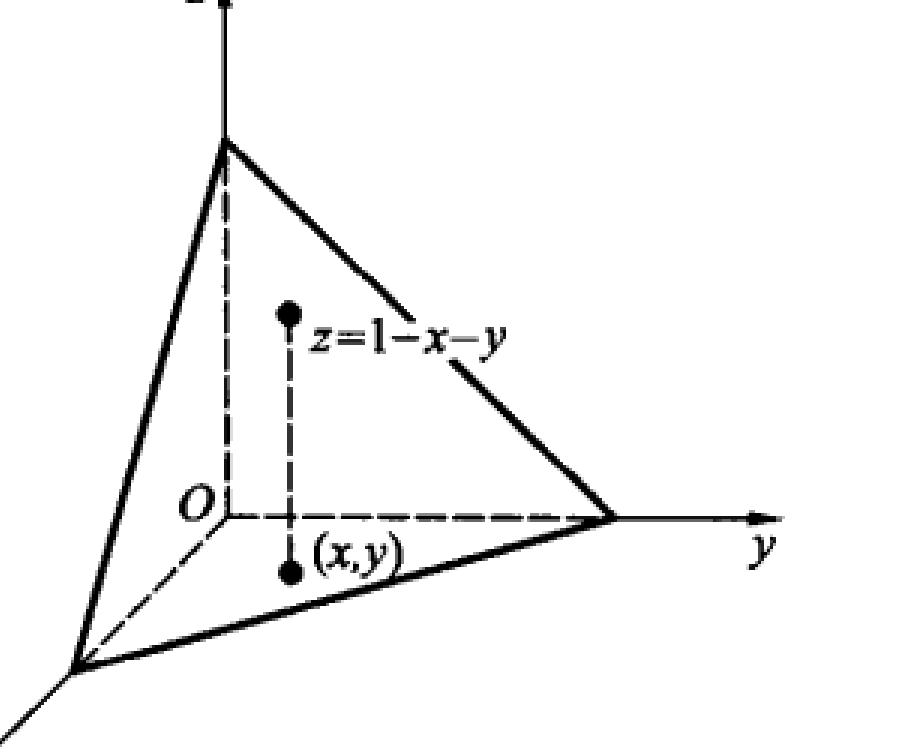
\includegraphics[width=0.32\textwidth]{work/figures/fig20-17}\caption{\relax}\label{fig:20-17}
\end{figure}

\begin{example}\label{ex:20-2-7}
求 $\displaystyle I=\iiint_{V}(x^{2}+y^{2}+z^{2})\,\mathrm{d}x\,\mathrm{d}y\,\mathrm{d}z$，其中 $V$ 是椭球体
\[
\frac{x^{2}}{a^{2}}+\frac{y^{2}}{b^{2}}+\frac{z^{2}}{c^{2}}\leqslant 1.
\]
\end{example}

\begin{proof}[解]
作图．

\begin{figure}[htbp]
\centering
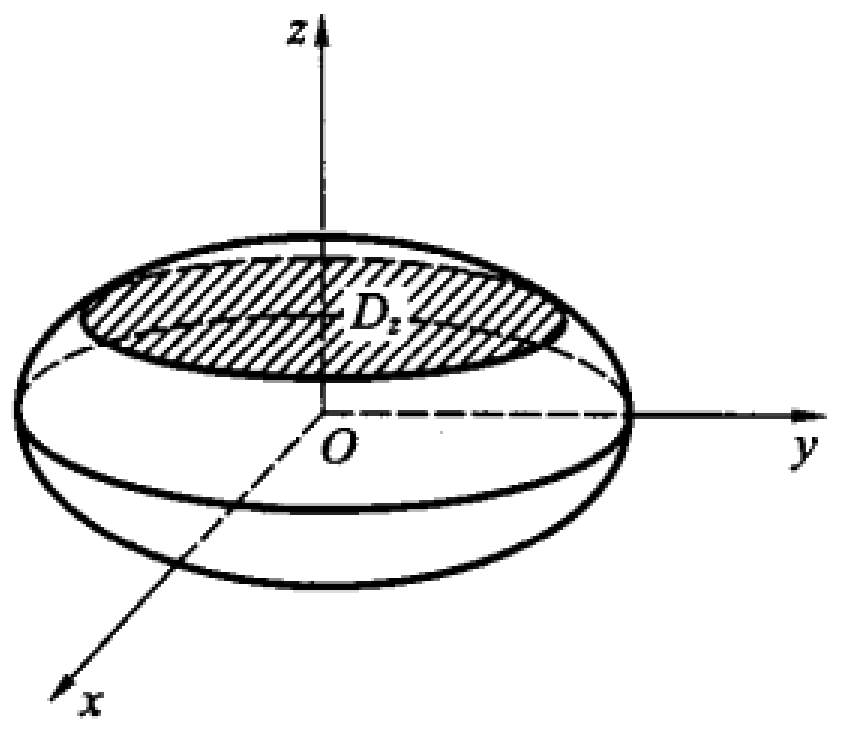
\includegraphics[width=0.32\textwidth]{work/figures/fig20-18}\caption{\relax}\label{fig:20-18}
\end{figure}

显然，对于每一 $z\in[-c,c]$，用平行于 $Oxy$ 面的平面 $z=z$ 去截椭球体，得一椭圆面 $D_{z}$：
\[
\frac{x^{2}}{a^{2}\left(1-\dfrac{z^{2}}{c^{2}}\right)}+\frac{y^{2}}{b^{2}\left(1-\dfrac{z^{2}}{c^{2}}\right)}\leqslant 1,
\]
它的面积为
\[
\pi\sqrt{a^{2}\left(1-\frac{z^{2}}{c^{2}}\right)}\cdot\sqrt{b^{2}\left(1-\frac{z^{2}}{c^{2}}\right)}=\pi ab\left(1-\frac{z^{2}}{c^{2}}\right).
\]
显然
\[
I=\iiint\limits_{V}x^{2}\,\mathrm{d}x\mathrm{d}y\mathrm{d}z+\iiint\limits_{V}y^{2}\,\mathrm{d}x\mathrm{d}y\mathrm{d}z+\iiint\limits_{V}z^{2}\,\mathrm{d}x\mathrm{d}y\mathrm{d}z.
\]
由前面的公式有
\[
\iiint_{V}z^{2}\,\mathrm{d}x\mathrm{d}y\mathrm{d}z=\int_{-c}^{c}z^{2}\,\mathrm{d}z\iint_{D_{z}}\mathrm{d}x\mathrm{d}y.
\]
根据二重积分的几何意义知，$\displaystyle\iint_{D_{z}}\mathrm{d}x\,\mathrm{d}y=D_{z}$ 的面积．因此
\[
\begin{aligned}
\iiint_{V}z^{2}\,\mathrm{d}x\mathrm{d}y\mathrm{d}z&=\int_{-c}^{c}z^{2}\pi ab\left(1-\frac{z^{2}}{c^{2}}\right)\mathrm{d}z\\
&=2\pi ab\int_{0}^{c}\left(z^{2}-\frac{1}{c^{2}}z^{4}\right)\mathrm{d}z=\frac{4}{15}\pi abc^{3}.
\end{aligned}
\]
由椭球体的对称性易见
\[
\iiint_{V}x^{2}\,\mathrm{d}x\mathrm{d}y\mathrm{d}z=\frac{4}{15}\pi a^{3}bc;\qquad
\iiint_{V}y^{2}\,\mathrm{d}x\mathrm{d}y\mathrm{d}z=\frac{4}{15}\pi ab^{3}c.
\]
于是
\[
I=\iiint\limits_{V}(x^{2}+y^{2}+z^{2})\,\mathrm{d}x\mathrm{d}y\mathrm{d}z=\frac{4}{15}\pi abc(a^{2}+b^{2}+c^{2}).
\]
\end{proof}

在上例的求解过程中，我们用到了以下一些技巧，使计算大大简化了．

（1）利用积分域的对称性和被积函数的对称性，只需计算三项积分中的一项．

（2）我们选择了最后对 $z$ 积分，即
\[
\iiint_{V}z^{2}\,\mathrm{d}x\mathrm{d}y\mathrm{d}z=\int_{-c}^{c}z^{2}\,\mathrm{d}z\iint_{D_{z}}\mathrm{d}x\mathrm{d}y,
\]
是因为一方面被积函数仅是 $z$ 的函数而不依赖于 $x$ 和 $y$，另一方面 $\displaystyle\iint_{D_{z}}\mathrm{d}x\,\mathrm{d}y$ 的值可利用二重积分的几何意义直接得到．

总之在求重积分时，应同时兼顾到积分域和被积函数的特点，合理地选择积分次序，尽可能简化计算．

\begin{xiti}
\item 计算下列二重积分：
\begin{ziti}
\item $\displaystyle\iint_{D}(y-2x)\,\mathrm{d}x\mathrm{d}y$，$\quad D=[3,5]\times[1,2]$；
\item $\displaystyle\iint_{D}\cos(x+y)\,\mathrm{d}x\,\mathrm{d}y$，$\quad D=\left[0,\dfrac{\pi}{2}\right]\times[0,\pi]$；
\item $\displaystyle\iint_{D}xy\mathrm{e}^{x^{2}+y^{2}}\,\mathrm{d}x\mathrm{d}y$，$D=[a,b]\times[c,d]$；
\item $\displaystyle\iint_{D}\frac{x}{1+xy}\,\mathrm{d}x\,\mathrm{d}y$，$\quad D=[0,1]\times[0,1]$．
\end{ziti}
\item 将二重积分 $\displaystyle\iint_{D}f(x,y)\,\mathrm{d}x\,\mathrm{d}y$ 化为不同顺序的累次积分：
\begin{ziti}
\item $D$ 由 $x$ 轴与 $x^{2}+y^{2}=r^{2}$ $(y>0)$ 所围成；
\item $D$ 由 $y=x$，$x=2$ 及 $y=\dfrac{1}{x}$ $(x>0)$ 所围成；
\item $D$ 由 $y=x^{3}$，$y=2x^{3}$，$y=1$ 和 $y=2$ 围成；
\item $D=\left\{(x,y)\mid \left|x\right|+\left|y\right|\leqslant 1\right\}$．
\end{ziti}
\item 改变下列累次积分的次序：
\begin{ziti}
\item $\displaystyle\int_{0}^{2}\mathrm{d}y\int_{y^{2}}^{3y}f(x,y)\,\mathrm{d}x$；
\item $\displaystyle\int_{1}^{2}\mathrm{d}x\int_{\sqrt{x}}^{2}f(x,y)\,\mathrm{d}y$；
\item $\displaystyle\int_{0}^{1}\mathrm{d}x\int_{0}^{x^{2}}f(x,y)\,\mathrm{d}y+\int_{1}^{3}\mathrm{d}x\int_{0}^{\frac{1}{2}(3-x)}f(x,y)\,\mathrm{d}y$．
\end{ziti}
\item 设 $f(x,y)$ 在所积分的区域 $D$ 上连续，证明
\[
\int_{a}^{b}\mathrm{d}x\int_{a}^{x}f(x,y)\,\mathrm{d}y=\int_{a}^{b}\mathrm{d}y\int_{y}^{b}f(x,y)\,\mathrm{d}x.
\]
\item 计算下列二重积分：
\begin{ziti}
\item $\displaystyle\iint_{D}x^{m}y^{k}\,\mathrm{d}x\,\mathrm{d}y$ $(m,k>0)$，$D$ 是由 $y=\sqrt{2px}$ $(p>0)$，$y=0$，$x=\dfrac{p}{2}$ 围成的区域；
\item $\displaystyle\iint_{D}x\,\mathrm{d}x\,\mathrm{d}y$，$D$ 是由 $y=0$，$y=\sin x^{2}$，$x=0$ 和 $x=\sqrt{\pi}$ 围成的区域；
\item $\displaystyle\iint_{D}\sqrt{x}\,\mathrm{d}x\,\mathrm{d}y$，$D$：$x^{2}+y^{2}\leqslant x$；
\item $\displaystyle\iint_{D}\left|xy\right|\,\mathrm{d}x\,\mathrm{d}y$，$D$：$x^{2}+y^{2}\leqslant a^{2}$；
\item $\displaystyle\iint_{D}(x+y)\,\mathrm{d}x\mathrm{d}y$，$D$ 由 $y=\mathrm{e}^{x}$，$y=1$，$x=0$，$x=1$ 所围成；
\item $\displaystyle\iint_{D}x^{2}y^{2}\,\mathrm{d}x\mathrm{d}y$，$D$ 由 $x=y^{2}$，$x=0$，$x=2$，$y=2+x$ 所围成；
\item $\displaystyle\iint_{D}\mathrm{e}^{x+y}\,\mathrm{d}x\mathrm{d}y$，$D$ 是以 $(2,2)$，$(2,3)$ 和 $(3,1)$ 为顶点的三角形；
\item $\displaystyle\iint_{D}\sin nx\,\mathrm{d}x\,\mathrm{d}y$，$D$ 由 $\sqrt{y}=x$，$y=4x$ 和 $y=4$ 所围成．
\end{ziti}
\item 求下列二重积分：
\begin{ziti}
\item $\displaystyle I=\int_{0}^{1}\mathrm{d}x\int_{x}^{1}\mathrm{e}^{-y^{2}}\,\mathrm{d}y$；
\item $\displaystyle I=\int_{0}^{1}\mathrm{d}x\int_{x}^{1}x^{2}\mathrm{e}^{-y^{2}}\,\mathrm{d}y$；
\item $\displaystyle I=\int_{0}^{\sqrt{\frac{\pi}{2}}}\mathrm{d}y\int_{y}^{\sqrt{\frac{\pi}{2}}}y^{2}\sin x^{2}\,\mathrm{d}x$．
\end{ziti}
\item 设 $y$ 轴将平面有界区域 $D$ 分成对称的两部分 $D_{1}$ 和 $D_{2}$，证明：
\begin{ziti}
\item 若 $f(x,y)$ 关于 $x$ 为奇函数，即 $f(-x,y)=-f(x,y)$，则
\[
\iint_{D}f(x,y)\,\mathrm{d}x\mathrm{d}y=0;
\]
\item 若 $f(x,y)$ 关于 $x$ 为偶函数，即 $f(-x,y)=f(x,y)$，则
\[
\iint_{D}f(x,y)\,\mathrm{d}x\mathrm{d}y=2\iint_{D_{1}}f(x,y)\,\mathrm{d}x\mathrm{d}y=2\iint_{D_{2}}f(x,y)\,\mathrm{d}x\mathrm{d}y.
\]
\end{ziti}
\item 计算下列三重积分：
\begin{ziti}
\item $\displaystyle\iiint_{V}(x+y+z)\,\mathrm{d}x\,\mathrm{d}y\,\mathrm{d}z$，$V$：$x^{2}+y^{2}+z^{2}\leqslant a^{2}$；
\item $\displaystyle\iiint_{V}z\,\mathrm{d}x\,\mathrm{d}y\,\mathrm{d}z$，$V$ 由曲面 $z=x^{2}+y^{2}$，$z=1$，$z=2$ 所围成；
\item $\displaystyle\iiint_{V}(1+x^{4})\,\mathrm{d}x\mathrm{d}y\mathrm{d}z$，$V$ 由曲面 $x^{2}=z^{2}+y^{2}$，$x=2$，$x=4$ 所围成；
\item $\displaystyle\iiint_{V}x^{3}yz\,\mathrm{d}x\,\mathrm{d}y\,\mathrm{d}z$，$V$ 是由曲面 $x^{2}+y^{2}+z^{2}=1$，$x=0$，$y=0$，$z=0$ 围成的位于第一卦限的有界区域；
\item $\displaystyle\iiint_{V}xy^{2}z^{3}\,\mathrm{d}x\mathrm{d}y\mathrm{d}z$，$V$ 由曲面 $z=xy$，$y=x$，$z=0$，$x=1$ 所围成；
\item $\displaystyle\iiint_{V}y\cos(x+z)\,\mathrm{d}x\,\mathrm{d}y\,\mathrm{d}z$，$V$ 是由 $y=\sqrt{x}$，$y=0$，$z=0$ 及 $x+z=\dfrac{\pi}{2}$ 所围成．
\end{ziti}
\item 改变下列累次积分的次序：
\begin{ziti}
\item $\displaystyle\int_{0}^{1}\mathrm{d}x\int_{0}^{1-x}\mathrm{d}y\int_{0}^{x+y}f(x,y,z)\,\mathrm{d}z$；
\item $\displaystyle\int_{0}^{1}\mathrm{d}x\int_{0}^{1}\mathrm{d}y\int_{0}^{x^{2}+y^{2}}f(x,y,z)\,\mathrm{d}z$；
\item $\displaystyle\int_{1}^{2}\mathrm{d}x\int_{0}^{1}\mathrm{d}y\int_{1-x-y}^{0}f(x,y,z)\,\mathrm{d}z$；
\item $\displaystyle\int_{-1}^{1}\mathrm{d}x\int_{-\sqrt{1-x^{2}}}^{\sqrt{1-x^{2}}}\mathrm{d}y\int_{\sqrt{x^{2}+y^{2}}}^{1}f(x,y,z)\,\mathrm{d}z$．
\end{ziti}
\item 求下列立体之体积：
\begin{ziti}
\item $V$ 由 $x^{2}+y^{2}+z^{2}\leqslant r^{2}$，$x^{2}+y^{2}+z^{2}\leqslant 2rz$ 所确定；
\item $V$ 由 $z\geqslant x^{2}+y^{2}$，$y\geqslant x^{2}$，$z\leqslant 2$ 所确定；
\item $V$ 是由坐标平面及 $x=2$，$y=3$，$x+y+z=4$ 所围成的角柱体．
\end{ziti}
\end{xiti}

\section{重积分的变量代换}\label{sec:20-3}

我们已经知道，变量代换即积分换元在定积分计算中占有重要的地位．定积分的变量代换公式说，若 $f(x)$ 在 $[a,b]$ 连续，变量代换 $x=\varphi(t)$ 在 $\alpha\leqslant t\leqslant\beta$ 可微，$\varphi(\alpha)=a$，$\varphi(\beta)=b$，则
\[
\int_{a}^{b}f(x)\,\mathrm{d}x=\int_{\alpha}^{\beta}f(\varphi(t))\varphi'(t)\,\mathrm{d}t.
\]
公式证明用的是微积分基本定理．设 $F(x)$ 是 $f(x)$ 的原函数，则 $F(\varphi(t))$ 是 $f(\varphi(t))\varphi'(t)$ 的原函数，因此
\[
\begin{aligned}
\int_{a}^{b}f(x)\,\mathrm{d}x&=F(b)-F(a)=F(\varphi(\beta))-F(\varphi(\alpha))\\
&=\int_{\alpha}^{\beta}f(\varphi(t))\varphi'(t)\,\mathrm{d}t.
\end{aligned}
\]
我们本节的目的，是把上述定积分的变量代换公式推广到重积分，其重要性读者以后将会看到．这是由于在重积分计算中，变量代换不仅有可能使被积函数简化，还可以使积分区域变得规则很多，从而使化累次积分变得容易而把积分计算出来．

然而重积分的变量代换公式应是什么样的？其证明又用什么方法？显然，到现在为止，在重积分中还没有微积分基本定理可以应用．因此只能回到积分的定义来考虑．下面主要以二重积分为例进行讨论．

\subsection{二重积分的变量代换}

考虑计算二重积分
\begin{equation}\label{eq:20-3-1}
\iint_{D}f(x,y)\,\mathrm{d}x\mathrm{d}y,
\tag{1}
\end{equation}
其中 $f(x,y)$ 在 $D$ 连续．而为了简单起见，设 $D$ 是由逐段光滑的简单闭曲线围成的．作变量代换
\begin{equation}\label{eq:20-3-2}
\begin{cases}
x=\varphi(u,v),\\
y=\psi(u,v),
\end{cases}
\tag{2}
\end{equation}
我们把它看作一个由平面 $Ouv$ 到平面 $Oxy$ 的映射 $T$．$T$ 通过\eqref{eq:20-3-2}的变换，把 $Ouv$ 平面的区域 $\Delta$ 映射成 $Oxy$ 平面的区域 $D$，即 $T$：$\Delta\to D$（图~\ref{fig:20-19}）．

\begin{figure}[htbp]
\centering
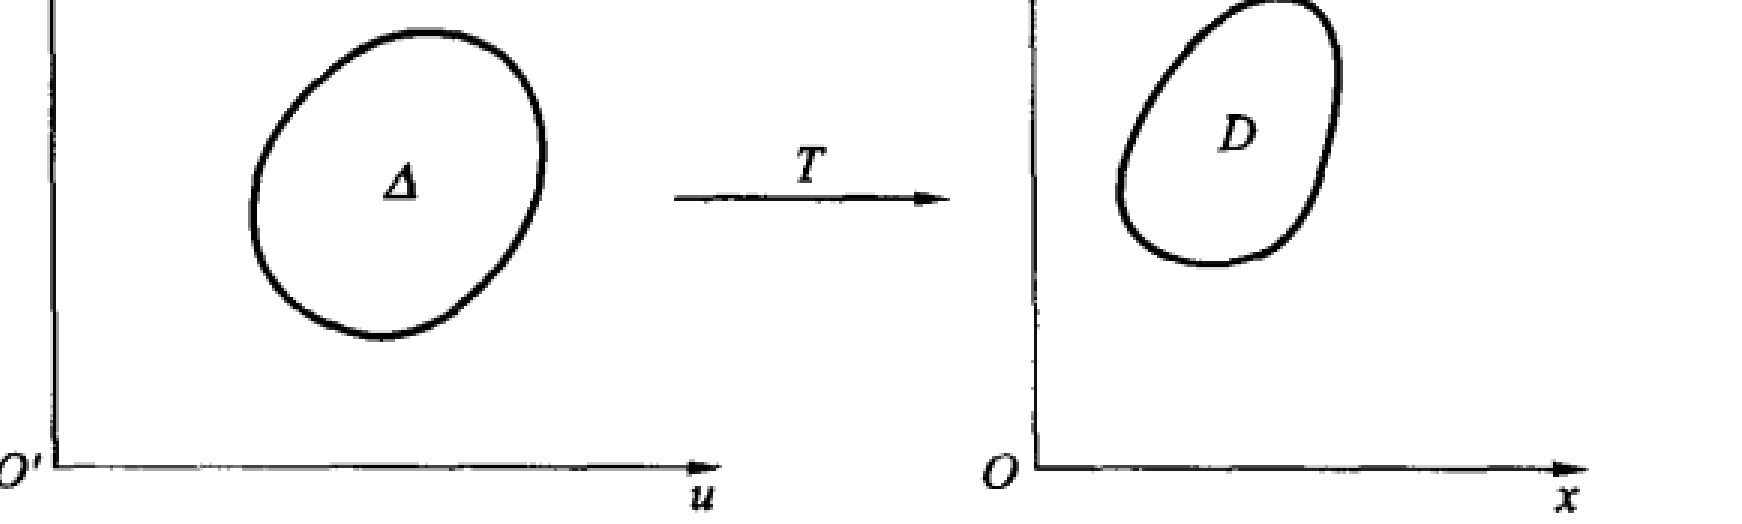
\includegraphics[width=0.72\textwidth]{work/figures/fig20-19}\caption{\relax}\label{fig:20-19}
\end{figure}

假设 $\varphi$，$\psi$ 在 $\Delta$ 有连续的二阶偏导数．显然，重积分换元公式不可能是把\eqref{eq:20-3-2}代入\eqref{eq:20-3-1}得到，因为若把 $\mathrm{d}x$，$\mathrm{d}y$ 看作微分的话，我们根本就不知道
\[
\iint\limits_{\Delta}f\left(\varphi(u,v),\psi(u,v)\right)\left(\frac{\partial\varphi}{\partial u}\mathrm{d}u+\frac{\partial\varphi}{\partial v}\mathrm{d}v\right)\left(\frac{\partial\psi}{\partial u}\mathrm{d}u+\frac{\partial\psi}{\partial v}\mathrm{d}v\right)
\]
表示什么？实际上当时用\eqref{eq:20-3-1}表示重积分，完全是一个记号，并说明没有理由把 $\mathrm{d}x\mathrm{d}y$ 看作是微分的乘积．

下面进一步，假设变换的函数行列式不取零值，即
\[
J(u,v)=\frac{\partial(x,y)}{\partial(u,v)}=\begin{vmatrix}
\dfrac{\partial\varphi}{\partial u} & \dfrac{\partial\varphi}{\partial v}\\[8pt]
\dfrac{\partial\psi}{\partial u} & \dfrac{\partial\psi}{\partial v}
\end{vmatrix}
\]
在 $\Delta$ 内没有零点．由于所有偏导数在 $\Delta$ 连续，因此 $\dfrac{\partial(x,y)}{\partial(u,v)}$ 恒为正或恒为负．

这时 $T\colon\Delta\to D$ 把 $\Delta$ 的内点映为 $D$ 的内点，并且是一一对应的，同时把 $\Delta$ 的边界点映为 $D$ 的边界点．这时，二重积分的变量代换公式是
\[
\iint\limits_{D}f(x,y)\,\mathrm{d}x\mathrm{d}y=\iint\limits_{\Delta}f\left(\varphi(u,v),\psi(u,v)\right)\left|J(u,v)\right|\,\mathrm{d}u\mathrm{d}v.
\]

为证明此公式，先证明下面的引理．

\begin{lemma}\label{lem:20-3-1}
设 $\sigma$ 是 $\Delta$ 内的一个正方形，左下方顶点为 $(u_{0},v_{0})$，边长为 $h$（图~\ref{fig:20-20}），经 $T$ 映为 $D$ 内的一个曲边四边形，记为 $S$，则 $S$ 的面积
\begin{equation}\label{eq:20-3-3}
\left|S\right|=\iint\limits_{\sigma}\left|J(u,v)\right|\,\mathrm{d}u\mathrm{d}v.
\tag{3}
\end{equation}
\end{lemma}

\begin{figure}[htbp]
\centering
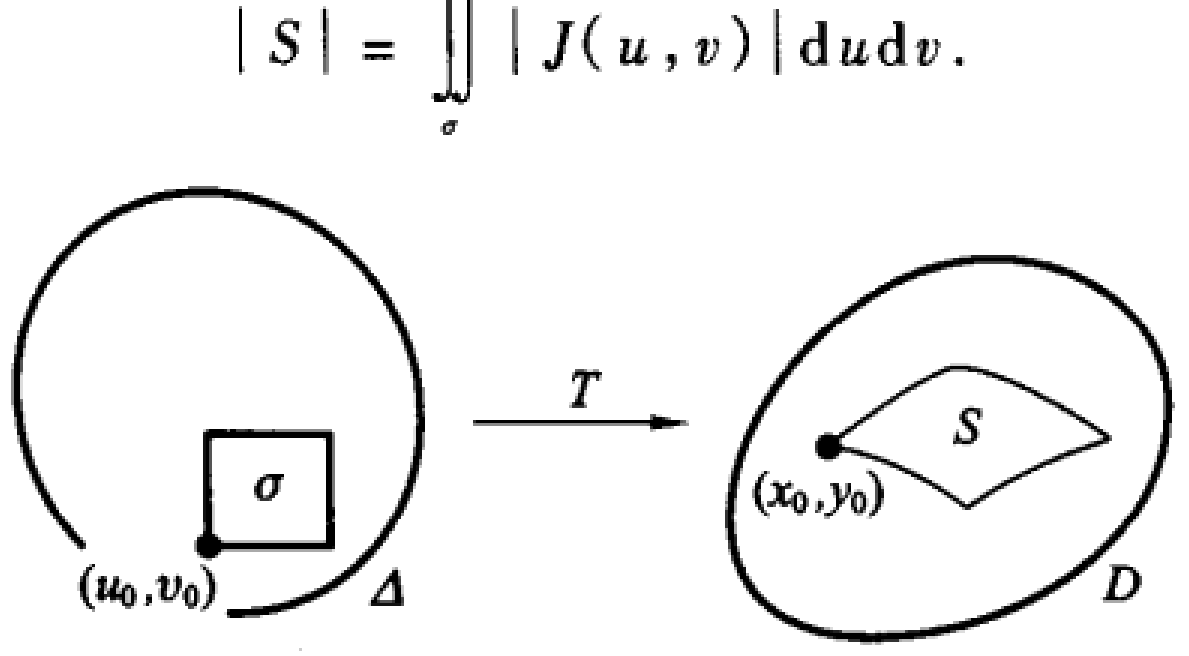
\includegraphics[width=0.55\textwidth]{work/figures/fig20-20}\caption{\relax}\label{fig:20-20}
\end{figure}

\begin{proof}
先设 $J(u,v)>0$．记 $\sigma$ 的边界为 $L$，$S$ 的边界为 $\mathcal{L}$．这时 $\mathcal{L}$ 可以分成四段，第一段的参数方程为
\[
\begin{cases}
x=\varphi(u,v_{0}),\\
y=\psi(u,v_{0}),
\end{cases}
\quad u_{0}\leqslant u\leqslant u_{0}+h,
\]
而第二段的参数方程为
\[
\begin{cases}
x=\varphi(u_{0}+h,v),\\
y=\psi(u_{0}+h,v),
\end{cases}
\quad v_{0}\leqslant v\leqslant v_{0}+h,
\]
其余两段可类似地写出．显然，$\mathcal{L}$ 在每段都是光滑的，因而是逐段光滑的．回忆定积分应用时讲授过的（第八章§2），如果简单逐段光滑闭曲线用参数方程给出，那么它所包围的面积为
\[
\left|S\right|=\frac{1}{2}\int_{\mathcal{L}}x\,\mathrm{d}y-y\,\mathrm{d}x,
\]
其中 $\mathcal{L}$ 的方向取正向．我们先按 $\mathcal{L}$ 是正向进行计算．把 $\mathcal{L}$ 四段的参数方程代入上式，得
\[
\begin{aligned}
2\left|S\right|&=\int_{u_{0}}^{u_{0}+h}\left[\varphi(u,v_{0})\frac{\partial\psi(u,v_{0})}{\partial u}-\psi(u,v_{0})\frac{\partial\varphi(u,v_{0})}{\partial u}\right]\mathrm{d}u+\\
&\ \int_{v_{0}}^{v_{0}+h}\left[\varphi(u_{0}+h,v)\frac{\partial\psi(u_{0}+h,v)}{\partial v}-\right.\\
&\ \left.\psi(u_{0}+h,v)\frac{\partial\varphi(u_{0}+h,v)}{\partial v}\right]\mathrm{d}v+\\
&\ \int_{u_{0}+h}^{u_{0}}\left[\varphi(u,v_{0}+h)\frac{\partial\psi(u,v_{0}+h)}{\partial u}-\right.\\
&\ \left.\psi(u,v_{0}+h)\frac{\partial\varphi(u,v_{0}+h)}{\partial u}\right]\mathrm{d}u+\\
&\ \int_{v_{0}+h}^{v_{0}}\left[\varphi(u_{0},v)\frac{\partial\psi(u_{0},v)}{\partial v}-\psi(u_{0},v)\frac{\partial\varphi(u_{0},v)}{\partial v}\right]\mathrm{d}v.
\end{aligned}
\]
把上面积分内的八项两两配对，并应用微积分基本定理，例如第一个积分的第一项与第三个积分的第一项相加，得
\[
\begin{aligned}
&-\int_{u_{0}}^{u_{0}+h}\left[\varphi(u,v_{0}+h)\frac{\partial\psi(u,v_{0}+h)}{\partial u}-\varphi(u,v_{0})\frac{\partial\psi(u,v_{0})}{\partial u}\right]\mathrm{d}u\\
=&-\int_{u_{0}}^{u_{0}+h}\mathrm{d}u\int_{v_{0}}^{v_{0}+h}\left[\frac{\partial\varphi(u,v)}{\partial v}\frac{\partial\psi(u,v)}{\partial u}+\varphi(u,v)\frac{\partial^{2}\psi(u,v)}{\partial v\partial u}\right]\mathrm{d}v\\
=&-\iint\limits_{\sigma}\left[\frac{\partial\varphi}{\partial v}\frac{\partial\psi}{\partial u}+\varphi\frac{\partial^{2}\psi}{\partial v\partial u}\right]\mathrm{d}u\mathrm{d}v,
\end{aligned}
\]
其中最后一个等式是根据重积分与累次积分的关系得到的．对其余六项同样处理，得
\[
\begin{aligned}
2\left|S\right|&=-\iint\limits_{\sigma}\left[\frac{\partial\varphi}{\partial v}\frac{\partial\psi}{\partial u}+\varphi\frac{\partial^{2}\psi}{\partial v\partial u}\right]\mathrm{d}u\mathrm{d}v+\iint\limits_{\sigma}\left[\frac{\partial\psi}{\partial v}\frac{\partial\varphi}{\partial u}+\psi\frac{\partial^{2}\varphi}{\partial v\partial u}\right]\mathrm{d}u\mathrm{d}v+\\
&\ \iint\limits_{\sigma}\left[\frac{\partial\varphi}{\partial u}\frac{\partial\psi}{\partial v}+\varphi\frac{\partial^{2}\psi}{\partial u\partial v}\right]\mathrm{d}u\mathrm{d}v-\iint\limits_{\sigma}\left[\frac{\partial\psi}{\partial u}\frac{\partial\varphi}{\partial v}+\psi\frac{\partial^{2}\varphi}{\partial u\partial v}\right]\mathrm{d}u\mathrm{d}v\\
&=2\iint\limits_{\sigma}\left|\begin{matrix}\dfrac{\partial\varphi}{\partial u}&\dfrac{\partial\varphi}{\partial v}\\[6pt]
\dfrac{\partial\psi}{\partial u}&\dfrac{\partial\psi}{\partial v}\end{matrix}\right|\mathrm{d}u\mathrm{d}v=2\iint\limits_{\sigma}J(u,v)\,\mathrm{d}u\mathrm{d}v.
\end{aligned}
\]
这时，由 $J(u,v)>0$，知上式右边取正值，与左边的面积连正负号都一致．这说明当初取 $\mathcal{L}$ 是正向的假定是正确的．当 $J(u,v)<0$ 时，作类似的计算，得
\[
2\left|S\right|=-\iint\limits_{\sigma}J(u,v)\,\mathrm{d}u\mathrm{d}v.
\]
总之我们得到了
\[
\left|S\right|=\iint\limits_{\sigma}\left|J(u,v)\right|\,\mathrm{d}u\mathrm{d}v
\]
的结论，这就完成了引理的证明．
\end{proof}

应用积分中值定理，知存在 $(\overline{u},\overline{v})\in\sigma$，使得
\begin{equation}\label{eq:20-3-4}
\left|S\right|=\left|J(\overline{u},\overline{v})\right|\left|\sigma\right|.
\tag{4}
\end{equation}
这个公式，我们是对 $\sigma$ 为正方形时证明的．实际上，当 $\sigma$ 是由逐段光滑闭曲线围成时，公式仍然正确．我们现在先承认这一点，读者以后学了格林公式之后便能更清楚地理解．

由公式\eqref{eq:20-3-4}，可以得到函数行列式的几何解释．事实上，在\eqref{eq:20-3-4}中令 $\sigma$ 的直径趋向于零，从而使 $\sigma$ 收缩为一点 $(u_{0},v_{0})$，由 $J(u,v)$ 的连续性，知
\[
\left|J(u_{0},v_{0})\right|=\lim_{d(\sigma)\to 0}\frac{\left|S\right|}{\left|\sigma\right|},
\]
也就是说，$J(u_{0},v_{0})$ 的绝对值，表示包含 $(u_{0},v_{0})$ 的简单闭曲线 $L$ 所包围的面积 $\left|\sigma\right|$，同 $L$ 在映射 $T$ 下的像 $\mathcal{L}$ 所包围的面积 $\left|S\right|$ 的比的极限，或简单说成是映射 $T$ 在 $(u_{0},v_{0})$ 的面积变化率．为解释其正负号的含义，回忆引~\ref{lem:20-3-1} 证明的过程，我们计算 $\left|\sigma\right|$ 与 $\left|S\right|$ 时，积分的顺序都是按 $L$ 与 $\mathcal{L}$ 的正向进行的，这时假定 $J(u,v)$ 为正，算出来的结果连正负号都是对的．因此，$J(u_{0},v_{0})>0$，表示在 $(u_{0},v_{0})$ 附近包含 $(u_{0},v_{0})$ 的闭曲线 $L$，在映射 $T$ 下的像 $\mathcal{L}$，它们是同向的（即 $L$ 取正向，$\mathcal{L}$ 也取正向；$L$ 取反向，$\mathcal{L}$ 也取反向）．而 $J(u_{0},v_{0})<0$ 则表示 $L$ 与 $\mathcal{L}$ 的方向是相反的（即若 $L$ 取正向，则 $\mathcal{L}$ 取反向；若 $L$ 取反向，则 $\mathcal{L}$ 取正向）．在这个意义下，把 $J(u,v)$ 看成微商概念在二维平面间的映射的推广是合理的．

现在，我们可以来证明二重积分的变量代换公式了．

\begin{theorem}\label{thm:20-3}
设变换 $T$：
\[
\begin{cases}
x=\varphi(u,v),\\
y=\psi(u,v)
\end{cases}
\]
把 $Ouv$ 平面上由逐段光滑的闭曲线围成的区域 $\Delta$ 一一地映射为 $Oxy$ 平面的区域 $D$，且 $\varphi$，$\psi$ 在 $\Delta$ 有二阶连续偏导数，
\[
J(u,v)=\frac{\partial(x,y)}{\partial(u,v)}\neq 0\quad\text{当}\ (u,v)\in\Delta,
\]
而 $f(x,y)$ 是定义在 $D$ 上的连续函数，则
\[
\iint_{D}f(x,y)\,\mathrm{d}x\mathrm{d}y=\iint_{\Delta}f\left(\varphi(u,v),\psi(u,v)\right)\left|J(u,v)\right|\,\mathrm{d}u\mathrm{d}v.
\]
\end{theorem}

\begin{proof}
用间隔为 $h$ 的平行于坐标轴的直线网，作 $\Delta$ 的一个分法：$\Delta\sigma_{1}$，$\Delta\sigma_{2}$，$\cdots$，$\Delta\sigma_{n}$，则通过映射 $T$ 便对应于 $D$ 的一个分法：$\Delta S_{1}$，$\Delta S_{2}$，$\cdots$，$\Delta S_{n}$．由公式\eqref{eq:20-3-4}知，存在 $(\bar{u}_{i},\bar{v}_{i})\in\Delta\sigma_{i}$，使得
\[
\left|\Delta S_{i}\right|=\left|J(\bar{u}_{i},\bar{v}_{i})\right|\left|\Delta\sigma_{i}\right|.
\]
记
\[
\begin{cases}
\bar{x}_{i}=\varphi(\bar{u}_{i},\bar{v}_{i}),\\
\bar{y}_{i}=\psi(\bar{u}_{i},\bar{v}_{i}),
\end{cases}
\]
显然 $(\bar{x}_{i},\bar{y}_{i})\in\Delta S_{i}$．作黎曼和
\[
\begin{aligned}
\sum_{i=1}^{n}f(\bar{x}_{i},\bar{y}_{i})\left|\Delta S_{i}\right|&=\sum_{i=1}^{n}f\left(\varphi(\bar{u}_{i},\bar{v}_{i}),\psi(\bar{u}_{i},\bar{v}_{i})\right)\left|\Delta S_{i}\right|\\
&=\sum_{i=1}^{n}f\left(\varphi(\bar{u}_{i},\bar{v}_{i}),\psi(\bar{u}_{i},\bar{v}_{i})\right)\left|J(\bar{u}_{i},\bar{v}_{i})\right|\left|\Delta\sigma_{i}\right|.
\end{aligned}
\]

\begin{figure}[htbp]
\centering
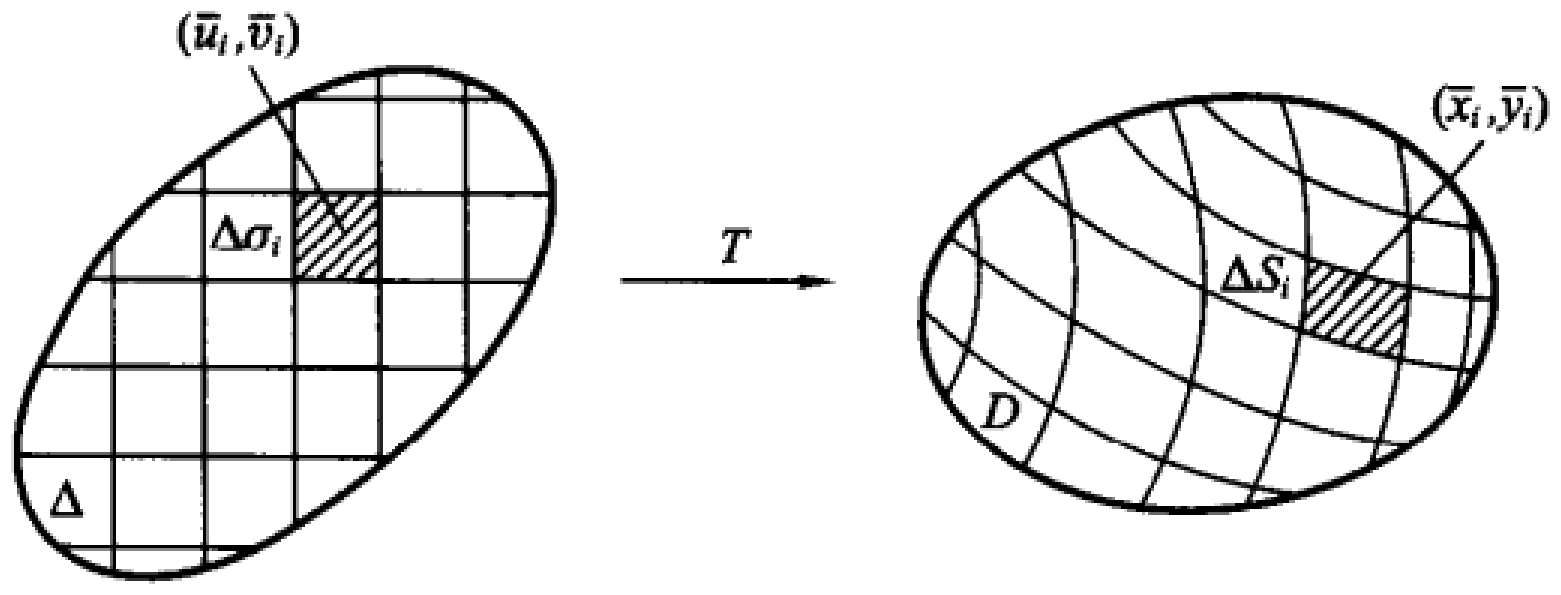
\includegraphics[width=0.68\textwidth]{work/figures/fig20-21}\caption{\relax}\label{fig:20-21}
\end{figure}

令 $h\to 0$，这时 $\lambda=\max\left(d(\Delta S_{i})\right)\to 0$，在上式两边取极限，便得
\[
\iint_{D}f(x,y)\,\mathrm{d}x\mathrm{d}y=\iint_{\Delta}f\left(\varphi(u,v),\psi(u,v)\right)\left|J(u,v)\right|\,\mathrm{d}u\mathrm{d}v.
\]
定理~\ref{thm:20-3}证完．
\end{proof}

从微元的观点来看，这公式是比较容易理解的．事实上，公式可以写成
\[
\iint_{D}f(x,y)\,\mathrm{d}S=\iint_{\Delta}f\left(\varphi(u,v),\psi(u,v)\right)\left|J(u,v)\right|\,\mathrm{d}\sigma.
\]
用平行于坐标轴的直线网作 $\Delta$ 的分法，相应地得到 $D$ 的用曲线网作成的分法，这时 $D$ 上的面积微元 $\mathrm{d}S$ 与 $\Delta$ 的面积微元 $\mathrm{d}\sigma$ 之间，按引理~\ref{lem:20-3-1}，有下列的关系
\begin{equation}\label{eq:20-3-5}
\mathrm{d}S=\left|J(u,v)\right|\mathrm{d}\sigma,
\tag{5}
\end{equation}
因此，相应地两边对 $f(P)$ 积分便得上述的换元公式．在这意义下，符号
\[
\iint_{D}f(P)\,\mathrm{d}S=\iint_{\Delta}f\left(\varphi(Q),\psi(Q)\right)\left|J(Q)\right|\,\mathrm{d}\sigma
\]
更能反映出变量代换中函数行列式是面积元之比的直观意义，但缺点是看不到积分变量，故通常还是写作
\[
\iint_{D}f(x,y)\,\mathrm{d}x\mathrm{d}y=\iint_{\Delta}f\left(\varphi(u,v),\psi(u,v)\right)\left|J(u,v)\right|\,\mathrm{d}u\mathrm{d}v,
\]
只要读者把
\[
\mathrm{d}x\mathrm{d}y=\left|J(u,v)\right|\mathrm{d}u\mathrm{d}v
\]
理解为\eqref{eq:20-3-5}的一种写法即可．

\begin{example}\label{ex:20-3-1}
计算二重积分
\[
\iint\limits_{D}xy\,\mathrm{d}x\mathrm{d}y,
\]
其中 $D$ 是由抛物线 $y^{2}=x$，$y^{2}=4x$，$x^{2}=y$，$x^{2}=4y$ 所围成的区域．
\end{example}

\begin{proof}[解]
画出 $D$ 的图形，根据 $D$ 的特点，作变换

\begin{figure}[htbp]
\centering
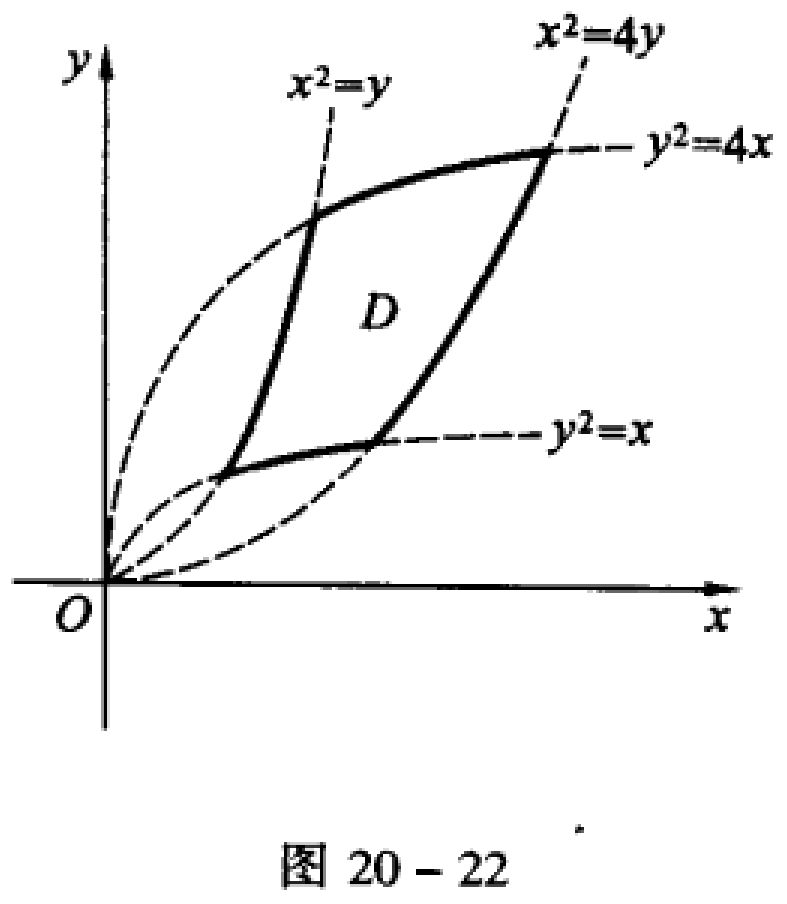
\includegraphics[width=0.30\textwidth]{work/figures/fig20-22}\caption{\relax}\label{fig:20-22}
\end{figure}
\[
T^{-1}:\quad u=\frac{y^{2}}{x},\quad v=\frac{x^{2}}{y},
\]
它把 $D$ 一一地映为正方形区域 $\Delta$：$1\leqslant u\leqslant 4$，$1\leqslant v\leqslant 4$．

计算
\[
\frac{\partial(u,v)}{\partial(x,y)}=\begin{vmatrix}
-\dfrac{y^{2}}{x^{2}} & \dfrac{2y}{x}\\[8pt]
\dfrac{2x}{y} & -\dfrac{x^{2}}{y^{2}}
\end{vmatrix}=-3.
\]
由于

\begin{figure}[htbp]
\centering
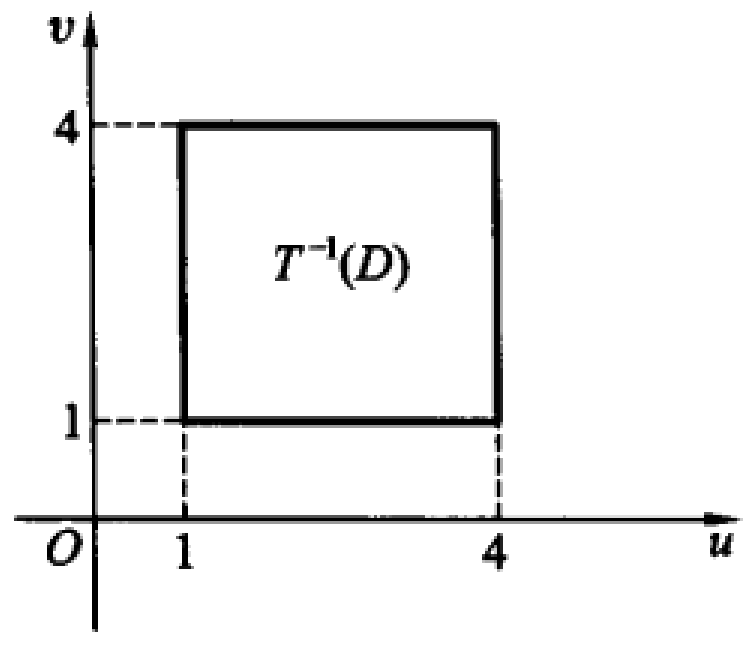
\includegraphics[width=0.28\textwidth]{work/figures/fig20-23}\caption{\relax}\label{fig:20-23}
\end{figure}
\[
\frac{\partial(x,y)}{\partial(u,v)}\cdot\frac{\partial(u,v)}{\partial(x,y)}=1,
\]
知
\[
\left|J(u,v)\right|=\left|\frac{\partial(x,y)}{\partial(u,v)}\right|=\frac{1}{3}.
\]
而
\[
uv=\frac{y^{2}}{x}\cdot\frac{x^{2}}{y}=xy,
\]
因此
\[
\iint_{D}xy\,\mathrm{d}x\mathrm{d}y=\iint_{\Delta}uv\cdot\frac{1}{3}\,\mathrm{d}u\mathrm{d}v=\frac{1}{3}\int_{1}^{4}u\,\mathrm{d}u\int_{1}^{4}v\,\mathrm{d}v=\frac{75}{4}.
\]
\end{proof}

平面变量代换中最重要的一种是\emph{极坐标变换}：
\[
\begin{cases}
x=r\cos\theta,\\
y=r\sin\theta.
\end{cases}
\]
变换的函数行列式为
\[
\frac{\partial(x,y)}{\partial(r,\theta)}=\begin{vmatrix}
\cos\theta & -r\sin\theta\\
\sin\theta & r\cos\theta
\end{vmatrix}=r.
\]
这个变换使 $Oxy$ 平面以原点为心的圆变为 $Or\theta$ 平面的直线 $r=$ 常数，把 $Oxy$ 平面的射线变为 $Or\theta$ 平面的另一束直线 $\theta=$ 常数．因此，极坐标变换对 $D$ 为由圆周与射线围成的区域时比较有效．由于这时 $r$，$\theta$ 的几何意义比较明显，我们有时很容易便写出 $Or\theta$ 平面区域的积分限，而无需把 $\Delta$ 画出来．

\begin{example}\label{ex:20-3-2}
计算
\[
\iint_{D}\mathrm{e}^{-x^{2}-y^{2}}\,\mathrm{d}x\mathrm{d}y,
\]
其中 $D$ 由 $x$，$y$ 正半轴与单位圆周及半径为 $2$ 的同心圆围成．
\end{example}

\begin{proof}[解]
作极坐标变换
\[
\begin{cases}
x=r\cos\theta,\\
y=r\sin\theta.
\end{cases}
\]
从 $r$，$\theta$ 的几何意义立刻看出，对应于 $D$ 的 $r$，$\theta$ 为

\begin{figure}[htbp]
\centering
\begin{tikzpicture}[scale=1.15,baseline=(current bounding box.center)]
  \fill[gray!12] (0.85,0) arc (0:90:0.85) -- (0,2) arc (90:0:2) -- cycle;
  \draw[{-Latex}] (-0.25,0) -- (2.5,0) node[below left] {$x$};
  \draw[{-Latex}] (0,-0.25) -- (0,2.5) node[below left] {$y$};
  \draw (0.85,0) arc (0:90:0.85);
  \draw (2,0) arc (0:90:2);
  \node at (1.25,0.95) {$D$};
  \node[below] at (0.85,0) {$1$};
  \node[below] at (2,0) {$2$};
\end{tikzpicture}\caption{\relax}\label{fig:20-24}
\end{figure}
\[
1\leqslant r\leqslant 2,\quad 0\leqslant\theta\leqslant\frac{\pi}{2}.
\]
因此
\[
\begin{aligned}
\iint_{D}\mathrm{e}^{-x^{2}-y^{2}}\,\mathrm{d}x\mathrm{d}y&=\int_{0}^{\frac{\pi}{2}}\mathrm{d}\theta\int_{1}^{2}\mathrm{e}^{-r^{2}}r\,\mathrm{d}r\\
&=\frac{\pi}{2}\int_{1}^{2}r\mathrm{e}^{-r^{2}}\,\mathrm{d}r=-\frac{\pi}{4}\mathrm{e}^{-r^{2}}\bigg|_{1}^{2}=\frac{\pi}{4}\left(\mathrm{e}^{-1}-\mathrm{e}^{-4}\right).
\end{aligned}
\]
\end{proof}

回忆定理~\ref{thm:20-3} 的证明，对极坐标变换来说，在公式
\begin{equation}\label{eq:20-3-6}
\iint\limits_{D}f(x,y)\,\mathrm{d}x\mathrm{d}y=\iint\limits_{\Delta}f\left(r\cos\theta,r\sin\theta\right)r\,\mathrm{d}r\mathrm{d}\theta
\tag{6}
\end{equation}
的证明中，对 $D$ 实际上是用 $\theta=$ 常数与 $r=$ 常数的两束曲线作分法（图~\ref{fig:20-25}）．从微元法的观点来看，这时的面积微元为（图~\ref{fig:20-26}）

\begin{figure}[htbp]
\centering
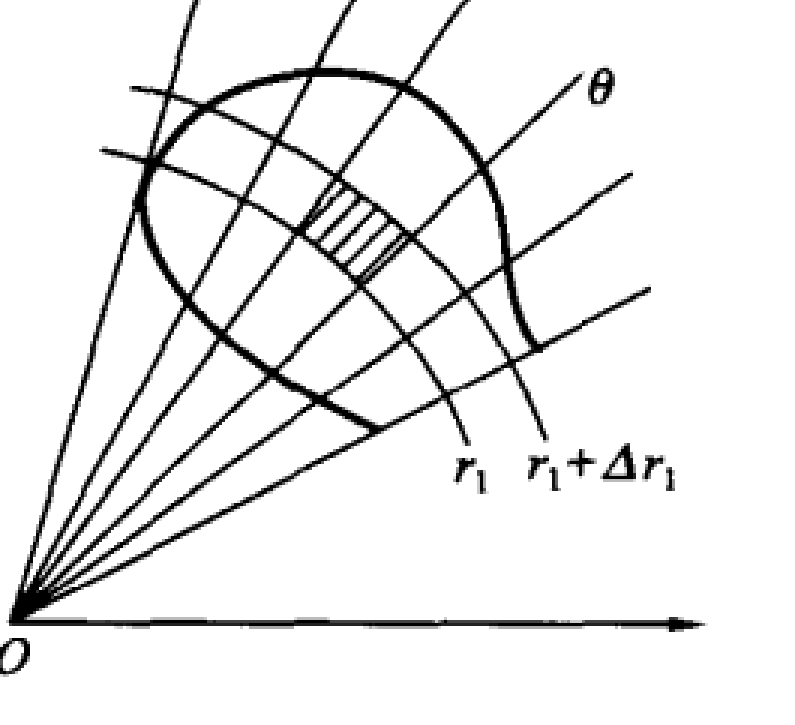
\includegraphics[width=0.30\textwidth]{work/figures/fig20-25}\caption{\relax}\label{fig:20-25}
\end{figure}

\begin{figure}[htbp]
\centering
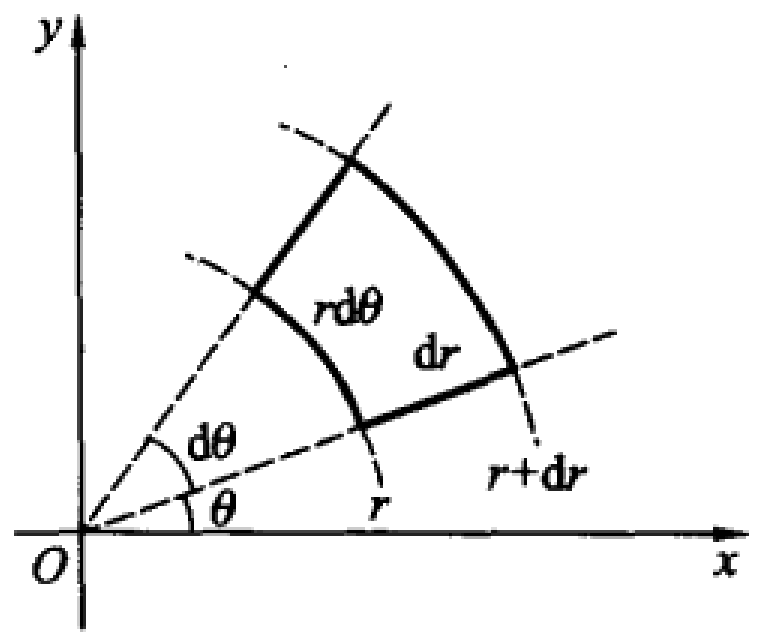
\includegraphics[width=0.30\textwidth]{work/figures/fig20-26}\caption{\relax}\label{fig:20-26}
\end{figure}
\[
\mathrm{d}S=r\,\mathrm{d}r\mathrm{d}\theta,
\]
因此，$D$ 上的函数 $f(x,y)$ 的积分自然应该等于微元
\[
f(r\cos\theta,r\sin\theta)\,r\,\mathrm{d}r\mathrm{d}\theta
\]
之和，这就是公式\eqref{eq:20-3-6}．

\begin{example}\label{ex:20-3-3}
利用二重积分变量代换计算概率积分
\[
\int_{0}^{+\infty}\mathrm{e}^{-x^{2}}\,\mathrm{d}x.
\]
\end{example}

\begin{proof}[解]
已知
\[
\int_{0}^{+\infty}\mathrm{e}^{-x^{2}}\,\mathrm{d}x=\lim_{a\to+\infty}\int_{0}^{a}\mathrm{e}^{-x^{2}}\,\mathrm{d}x.
\]
而
\[
\left(\int_{0}^{a}\mathrm{e}^{-x^{2}}\,\mathrm{d}x\right)^{2}=\int_{0}^{a}\mathrm{e}^{-x^{2}}\,\mathrm{d}x\int_{0}^{a}\mathrm{e}^{-y^{2}}\,\mathrm{d}y=\iint\limits_{D_{a}}\mathrm{e}^{-x^{2}-y^{2}}\,\mathrm{d}x\mathrm{d}y,
\]
其中 $D_{a}=[0,a]\times[0,a]$，右边的积分仍无法计算，引入
\[
\overline{D}_{a}=\left\{(x,y)\mid x^{2}+y^{2}\leqslant a^{2},x\geqslant 0,y\geqslant 0\right\},
\]
\[
\overline{\overline{D}}_{a}=\left\{(x,y)\mid x^{2}+y^{2}\leqslant 2a^{2},x\geqslant 0,y\geqslant 0\right\},
\]
则 $\overline{D}_{a}\subset D_{a}\subset\overline{\overline{D}}_{a}$．因为 $\mathrm{e}^{-x^{2}-y^{2}}\geqslant 0$，
\begin{equation}\label{eq:20-3-7}
\iint\limits_{\overline{D}_{a}}\mathrm{e}^{-x^{2}-y^{2}}\,\mathrm{d}x\mathrm{d}y\leqslant\iint\limits_{D_{a}}\mathrm{e}^{-x^{2}-y^{2}}\,\mathrm{d}x\mathrm{d}y\leqslant\iint\limits_{\overline{\overline{D}}_{a}}\mathrm{e}^{-x^{2}-y^{2}}\,\mathrm{d}x\mathrm{d}y.
\tag{7}
\end{equation}

\begin{figure}[htbp]
\centering
\begin{tikzpicture}[scale=1.05,baseline=(current bounding box.center)]
  \draw[{-Latex}] (-0.25,0) -- (2.6,0) node[below left] {$x$};
  \draw[{-Latex}] (0,-0.25) -- (0,2.6) node[below left] {$y$};
  \draw (0,2.2) -- (2.2,2.2) -- (2.2,0);
  \draw (1.556,0) arc (0:90:1.556);
  \draw (2.2,0) arc (0:90:2.2);
  \node[right] at (0.1,2.1) {\small $\overline{\overline{D}}_{a}$};
  \node at (1.35,1.35) {\small $D_{a}$};
  \node at (0.75,0.75) {\small $\overline{D}_{a}$};
  \node[below] at (1.556,0) {$a$};
  \node[below] at (2.2,0) {$\sqrt{2}\,a$};
\end{tikzpicture}\caption{\relax}\label{fig:20-27}
\end{figure}

而对不等式前后的两个积分，可以用极坐标变换计算
\[
\iint\limits_{\overline{D}_{a}}\mathrm{e}^{-x^{2}-y^{2}}\,\mathrm{d}x\mathrm{d}y=\int_{0}^{\frac{\pi}{2}}\mathrm{d}\theta\int_{0}^{a}r\mathrm{e}^{-r^{2}}\,\mathrm{d}r=\frac{\pi}{4}(1-\mathrm{e}^{-a^{2}}),
\]
\[
\iint\limits_{\overline{\overline{D}}_{a}}\mathrm{e}^{-x^{2}-y^{2}}\,\mathrm{d}x\mathrm{d}y=\frac{\pi}{4}(1-\mathrm{e}^{-2a^{2}}).
\]
代入\eqref{eq:20-3-7}中再令 $a\to+\infty$，用极限的夹逼定理，得
\[
\lim_{a\to+\infty}\iint_{D_{a}}\mathrm{e}^{-x^{2}-y^{2}}\,\mathrm{d}x\mathrm{d}y=\frac{\pi}{4},
\]
因此
\[
\int_{0}^{+\infty}\mathrm{e}^{-x^{2}}\,\mathrm{d}x=\frac{\sqrt{\pi}}{2}.
\]
\end{proof}

在第十九章 §2 中我们用无穷积分交换顺序计算过这个积分．显然，这里的计算要简便得多．

在上面计算积分
\[
\iint\limits_{\overline{D}_{a}}\mathrm{e}^{-x^{2}-y^{2}}\,\mathrm{d}x\mathrm{d}y
\]
的过程中，用了极坐标变换
\[
\begin{cases}
x=r\cos\theta,\\
y=r\sin\theta,
\end{cases}
\quad 0\leqslant\theta\leqslant\frac{\pi}{2},\ 0\leqslant r\leqslant a.
\]
这时函数行列式
\[
J(r,\theta)=r.
\]
在 $r=0$ 时为 $0$，不满足定理~\ref{thm:20-3} 的条件．而事实上，我们的计算仍然是正确的，它可以解释如下：用小扇形把原点挖去，引入区域
\[
D_{a\varepsilon}=\left\{(x,y)\mid\varepsilon^{2}\leqslant x^{2}+y^{2}\leqslant a^{2},x\geqslant 0,y\geqslant 0\right\},
\]

\begin{figure}[htbp]
\centering
\begin{tikzpicture}[scale=1.1,baseline=(current bounding box.center)]
  \draw[{-Latex}] (-0.25,0) -- (2.5,0) node[below left] {$x$};
  \draw[{-Latex}] (0,-0.25) -- (0,2.3) node[below left] {$y$};
  \draw (2,0) arc (0:90:2);
  \draw (0.35,0) arc (0:90:0.35);
  \fill[gray!12] (2,0) arc (0:90:2) -- (0,2) -- (0,0.35) arc (90:0:0.35) -- (0.35,0) -- cycle;
  \node at (1.1,1.1) {$D_{a\varepsilon}$};
  \node[below] at (0.35,0) {$\varepsilon$};
  \node[below] at (2,0) {$a$};
\end{tikzpicture}\caption{\relax}\label{fig:20-28}
\end{figure}

则 $J(r,\theta)$ 在 $D_{a\varepsilon}$ 不为 $0$，这时
\[
\begin{aligned}
\iint\limits_{\overline{D}_{a}}\mathrm{e}^{-x^{2}-y^{2}}\,\mathrm{d}x\mathrm{d}y&=\lim_{\varepsilon\to 0}\iint\limits_{D_{a\varepsilon}}\mathrm{e}^{-x^{2}-y^{2}}\,\mathrm{d}x\mathrm{d}y\\
&=\lim_{\varepsilon\to 0}\int_{0}^{\frac{\pi}{2}}\mathrm{d}\theta\int_{\varepsilon}^{a}r\mathrm{e}^{-r^{2}}\,\mathrm{d}r=\lim_{\varepsilon\to 0}\frac{\pi}{4}\left(\mathrm{e}^{-\varepsilon^{2}}-\mathrm{e}^{-a^{2}}\right)\\
&=\frac{\pi}{4}(1-\mathrm{e}^{-a^{2}}).
\end{aligned}
\]
至于在第一个等式中，左边等于右边的极限，是因为二者之差
\[
\iint_{\overline{D}_{a}\setminus D_{a\varepsilon}}\mathrm{e}^{-x^{2}-y^{2}}\,\mathrm{d}x\mathrm{d}y\leqslant\iint_{\overline{D}_{a}\setminus D_{a\varepsilon}}\mathrm{d}x\mathrm{d}y\leqslant\frac{\pi}{4}\varepsilon^{2}\to 0\quad(\varepsilon\to 0).
\]

从上述的证明看出，定理~\ref{thm:20-3} 中 $J(u,v)$ 在 $D$ 恒正或恒负的条件可减弱为 $J(u,v)\geqslant 0$，但只允许在 $\Delta$ 的有限个点上取 $0$ 值．事实上，这时可用有限个小圆把这些点挖去，再令这些圆的半径趋向于 $0$ 取极限．

\begin{example}\label{ex:20-3-4}
计算在旋转抛物面 $z=x^{2}+y^{2}$ 之下，$Oxy$ 平面 $z=0$ 之上，由圆柱面
\[
(x-a)^{2}+y^{2}=a^{2}
\]
截出的空间立体的体积．
\end{example}

\begin{proof}[解]
记平面区域
\[
D=\left\{(x,y)\mid(x-a)^{2}+y^{2}\leqslant a^{2}\right\},
\]
我们要计算的体积等于二重积分
\[
V=\iint\limits_{D}(x^{2}+y^{2})\,\mathrm{d}x\mathrm{d}y.
\]

\begin{figure}[htbp]
\centering
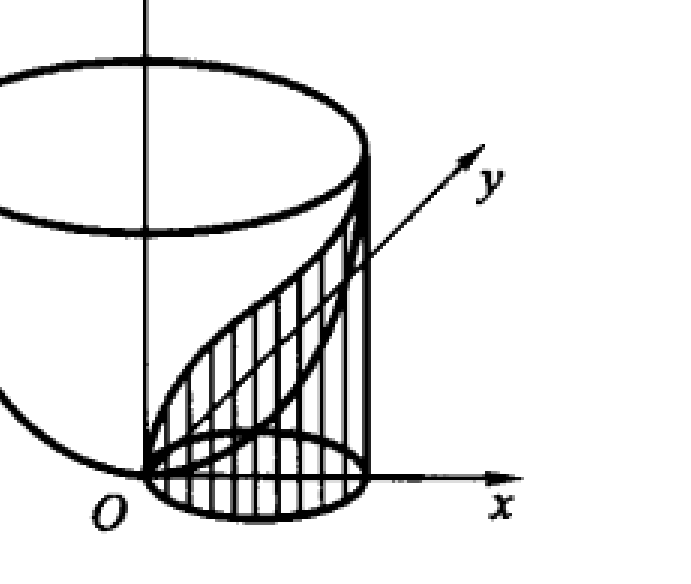
\includegraphics[width=0.30\textwidth]{work/figures/fig20-29}\caption{\relax}\label{fig:20-29}
\end{figure}

作极坐标变换
\[
\begin{cases}
x=r\cos\theta,\\
y=r\sin\theta.
\end{cases}
\]
这时对应于 $D$ 的极坐标（见图~\ref{fig:20-30}）为
\[
-\frac{\pi}{2}\leqslant\theta\leqslant\frac{\pi}{2},\quad 0\leqslant r\leqslant 2a\cos\theta.
\]

\begin{figure}[htbp]
\centering
\begin{tikzpicture}[scale=1.1,baseline=(current bounding box.center)]
  \draw[{-Latex}] (-1.1,0) -- (2.6,0) node[below left] {$x$};
  \draw[{-Latex}] (0,-1.1) -- (0,1.9) node[below left] {$y$};
  \draw (1,0) circle (1);
  \draw[thick] (0,0) -- (60:2) node[above right] {\small $\theta$};
  \node[below] at (2,0) {$2a$};
  \node[above] at (0.5,0.85) {$D$};
\end{tikzpicture}\caption{\relax}\label{fig:20-30}
\end{figure}

因此
\[
\begin{aligned}
\iint_{D}(x^{2}+y^{2})\,\mathrm{d}x\mathrm{d}y&=\int_{-\frac{\pi}{2}}^{\frac{\pi}{2}}\mathrm{d}\theta\int_{0}^{2a\cos\theta}r^{3}\,\mathrm{d}r\\
&=\int_{-\frac{\pi}{2}}^{\frac{\pi}{2}}\frac{1}{4}(2a\cos\theta)^{4}\,\mathrm{d}\theta\\
&=8a^{4}\int_{0}^{\frac{\pi}{2}}\cos^{4}\theta\,\mathrm{d}\theta=8a^{4}\cdot\frac{3\cdot 1}{4\cdot 2}\cdot\frac{\pi}{2}\\
&=\frac{3}{2}\pi a^{4}.
\end{aligned}
\]
\end{proof}

\begin{example}\label{ex:20-3-5}
求椭球体的体积 $V$．
\end{example}

\begin{proof}[解]
设椭球体为
\[
\frac{x^{2}}{a^{2}}+\frac{y^{2}}{b^{2}}+\frac{z^{2}}{c^{2}}\leqslant 1.
\]
则由对称性知

\begin{figure}[htbp]
\centering
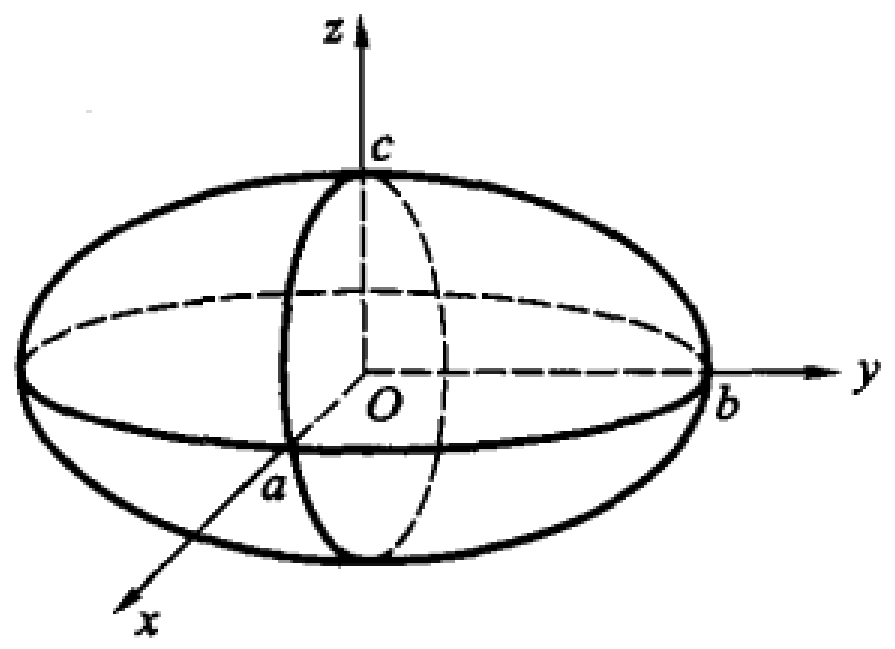
\includegraphics[width=0.34\textwidth]{work/figures/fig20-31}\caption{\relax}\label{fig:20-31}
\end{figure}
\[
V=2\iint_{D}c\sqrt{1-\frac{x^{2}}{a^{2}}-\frac{y^{2}}{b^{2}}}\,\mathrm{d}x\mathrm{d}y,
\]
其中
\[
D=\left\{(x,y)\mid\frac{x^{2}}{a^{2}}+\frac{y^{2}}{b^{2}}\leqslant 1\right\}.
\]
作广义极坐标变换
\[
x=ar\cos\theta,\quad y=br\sin\theta,
\]
则 $D$ 对应于 $0\leqslant r\leqslant 1$，$0\leqslant\theta\leqslant 2\pi$．而
\[
\frac{\partial(x,y)}{\partial(r,\theta)}=\begin{vmatrix}
a\cos\theta & -a\sin\theta\\
b\sin\theta & br\cos\theta
\end{vmatrix}=abr,
\]
因此
\[
\begin{aligned}
V&=2\int_{0}^{2\pi}\mathrm{d}\theta\int_{0}^{1}c\sqrt{1-r^{2}}\,abr\,\mathrm{d}r\\
&=4\pi abc\int_{0}^{1}\sqrt{1-r^{2}}\,r\,\mathrm{d}r=4\pi abc\cdot\frac{1}{2}\cdot\frac{2}{3}\left(1-r^{2}\right)^{\frac{3}{2}}\bigg|_{1}^{0}\\
&=\frac{4}{3}\pi abc.
\end{aligned}
\]
这比在直角坐标系下化累次积分计算要简单得多．
\end{proof}

\subsection{三重积分的变量代换}

三重积分的变量代换公式与二重积分变量代换公式完全类似．我们不再详细推导，在此仅给出公式的叙述．

设函数 $f(x,y,z)$ 在由逐片光滑曲面围成的闭区域 $V$ 上连续，变换 $T$
\[
\begin{cases}
x=x(u,v,w),\\
y=y(u,v,w),\\
z=z(u,v,w)
\end{cases}
\]
将 $Ouvw$ 坐标系下的区域 $\Omega$ 一一映射为 $V$．函数 $x(u,v,w)$，$y(u,v,w)$，$z(u,v,w)$ 在 $\Omega$ 有连续的二阶偏导数，且雅可比行列式
\[
J(u,v,w)=\frac{\partial(x,y,z)}{\partial(u,v,w)}\neq 0,
\]
则
\begin{equation}\label{eq:20-3-8}
\begin{aligned}
&\iiint\limits_{V}f(x,y,z)\,\mathrm{d}x\mathrm{d}y\mathrm{d}z\\
=&\iiint\limits_{\Omega}f\left(x(u,v,w),y(u,v,w),z(u,v,w)\right)\left|\frac{\partial(x,y,z)}{\partial(u,v,w)}\right|\mathrm{d}u\mathrm{d}v\mathrm{d}w.
\end{aligned}
\tag{8}
\end{equation}

公式的证明完全类似于二重积分的情形．即首先证明，函数行列式的大小 $\left|J(u_{0},v_{0},w_{0})\right|$ 实际上就是变换 $T$ 在 $(u_{0},v_{0},w_{0})$ 的体积变化率
\[
\left|J(u_{0},v_{0},w_{0})\right|=\lim\frac{\left|\Delta V\right|}{\Delta\Omega},
\]
其中 $\Delta\Omega$ 是包含 $(u_{0},v_{0},w_{0})$ 的小块体积，$\Delta V$ 是 $\Delta\Omega$ 在变换 $T$ 下的像，而极限过程是 $\Delta\Omega$ 收缩到点 $(u_{0},v_{0},w_{0})$．其次，是用 $u=$ 常数，$v=$ 常数与 $w=$ 常数的三组平行于坐标平面的平面作 $\Omega$ 的分法，这对应于用三束坐标曲面作 $V$ 的分法．这时
\[
\left|J(u,v,w)\right|\mathrm{d}u\mathrm{d}v\mathrm{d}w
\]
就是曲面坐标下的体积元，从而得到公式\eqref{eq:20-3-8}．

一般地，类似于二重积分，如果在有限个点，或有限条光滑曲线，或有限块光滑曲面上 $\dfrac{\partial(x,y,z)}{\partial(u,v,w)}=0$，而在 $V$ 的其余地方 $J(u,v,w)$ 不变号，则变量代换公式仍然成立．

三重积分最常用的变量代换有\emph{柱坐标变换}和\emph{球坐标变换}．分别介绍如下．

（1）柱坐标变换
\[
\begin{cases}
x=r\cos\theta, & 0\leqslant r<+\infty,\\
y=r\sin\theta, & 0\leqslant\theta<2\pi,\\
z=z, & -\infty<z<+\infty,
\end{cases}
\]
这时
\[
J(r,\theta,z)=\frac{\partial(x,y,z)}{\partial(r,\theta,z)}=\begin{vmatrix}
\cos\theta & -r\sin\theta & 0\\
\sin\theta & r\cos\theta & 0\\
0 & 0 & 1
\end{vmatrix}=r.
\]
因此变量代换公式为
\[
\iiint\limits_{V}f(x,y,z)\,\mathrm{d}x\mathrm{d}y\mathrm{d}z=\iiint\limits_{\Omega}f(r\cos\theta,r\sin\theta,z)\,r\,\mathrm{d}r\mathrm{d}\theta\mathrm{d}z.
\]

下面从微元的观点来看看这个公式．在 $Oxyz$ 空间中，柱坐标中的 $r$ 表示 $(x,y,z)$ 在 $Oxy$ 平面上的投影点 $P$ 与原点的距离，而 $\theta$ 则表原点和投影点 $P$ 连线 $OP$ 与 $x$ 轴正向的夹角．坐标曲面 $r=$ 常数是以 $z$ 轴为中心的圆柱面；$\theta=$ 常数是过 $z$ 轴的半平面；$z=$ 常数是垂直于 $z$ 轴的平面（图~\ref{fig:20-32}）．显然如果 $(x,y,z)$ 的柱坐标是 $(r,\theta,z)$，则 $(r,\theta)$ 就是 $(x,y)$ 的极坐标．

\begin{figure}[htbp]
\centering
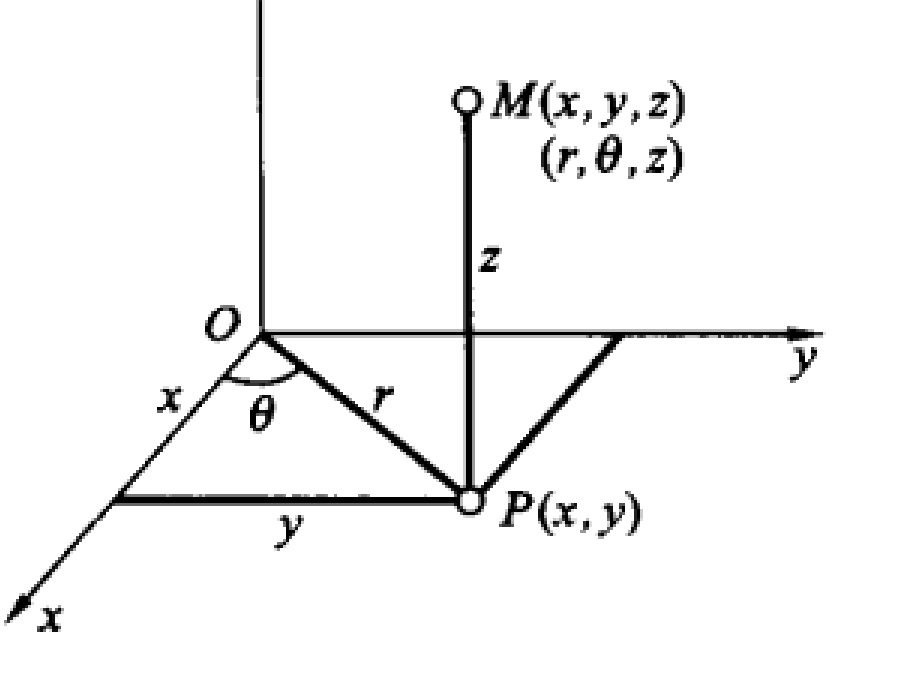
\includegraphics[width=0.32\textwidth]{work/figures/fig20-32}\caption{\relax}\label{fig:20-32}
\end{figure}

用柱坐标曲面网对 $V$ 作分法后，体积元的底面积近似于极坐标网下的面积元 $r\,\mathrm{d}r\,\mathrm{d}\theta$，而高为 $\mathrm{d}z$，因此在柱坐标下，体积元为 $r\,\mathrm{d}r\,\mathrm{d}\theta\,\mathrm{d}z$．这从图~\ref{fig:20-33} 看是显然的．

\begin{figure}[htbp]
\centering
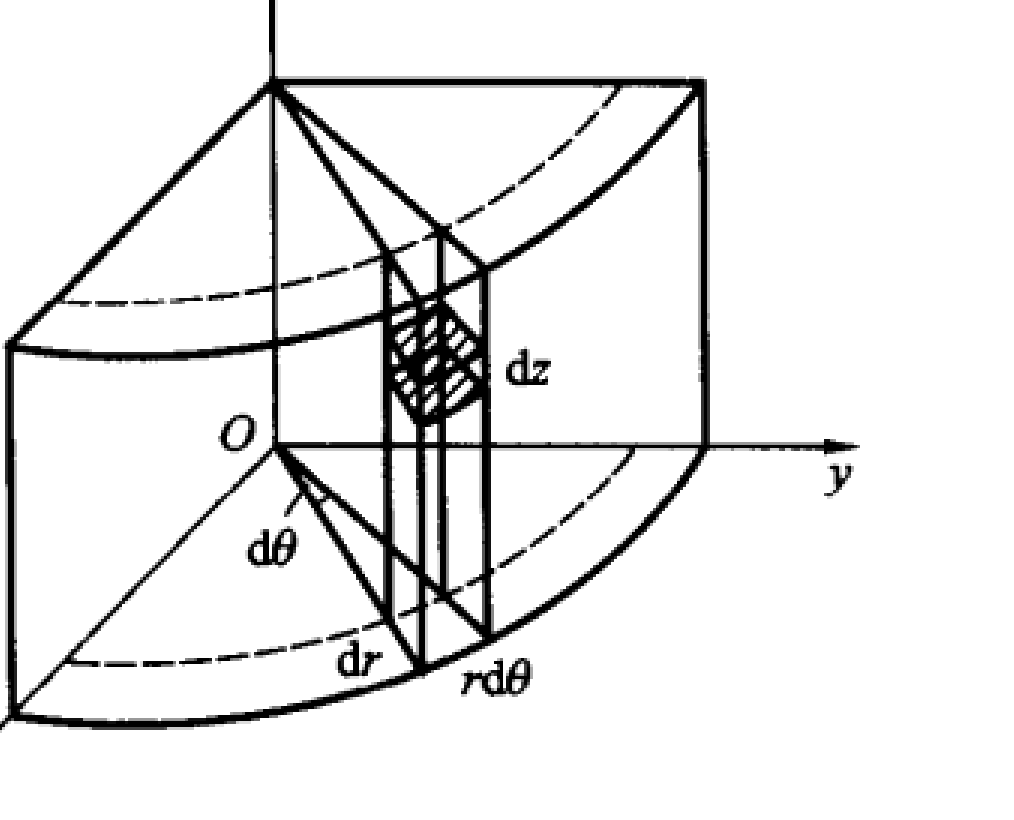
\includegraphics[width=0.36\textwidth]{work/figures/fig20-33}\caption{\relax}\label{fig:20-33}
\end{figure}

变量代换公式右边的积分通常化为累次积分来计算．将 $V$ 投影到 $Oxy$ 平面上，记该投影区域为 $D$，它的极坐标表示为 $\Delta$，则 $V$ 的柱坐标表示为
\[
\Omega=\left\{(r,\theta,z)\mid z_{1}(r,\theta)\leqslant z\leqslant z_{2}(r,\theta),(r,\theta)\in\Delta\right\}.
\]
因此
\[
\iiint_{V}f(x,y,z)\,\mathrm{d}x\mathrm{d}y\mathrm{d}z=\iint_{\Delta}r\,\mathrm{d}r\mathrm{d}\theta\int_{z_{1}(r,\theta)}^{z_{2}(r,\theta)}f(r\cos\theta,r\sin\theta,z)\,\mathrm{d}z.
\]

\begin{example}\label{ex:20-3-6}
求积分 $\displaystyle\iiint_{V}\frac{z}{\left(x^{2}+y^{2}+z^{2}\right)^{\frac{3}{2}}}\,\mathrm{d}x\mathrm{d}y\mathrm{d}z$．其中 $V$ 是柱面 $x^{2}+y^{2}=1$ 和锥面 $x^{2}+y^{2}=z^{2}$ $(z>0)$ 以及平面 $z=h$ $(h>1)$ 所围成的立体（见图~\ref{fig:20-34}）．
\end{example}

\begin{proof}[解]
作柱坐标变换
\[
x=r\cos\theta,\quad y=r\sin\theta,\quad z=z.
\]
则在柱坐标下，三曲面方程分别为 $r=1$，$r=z$，$z=h$，故 $V$ 在柱坐标下为
\[
\left\{(r,\theta,z)\mid r\leqslant z\leqslant h,0\leqslant r\leqslant 1,0\leqslant\theta\leqslant 2\pi\right\}.
\]

\begin{figure}[htbp]
\centering
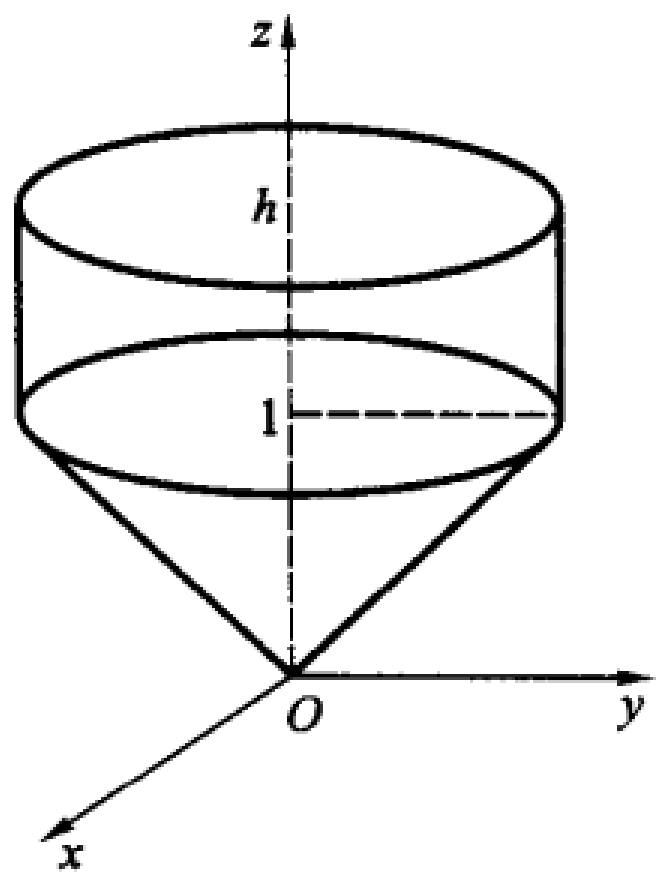
\includegraphics[width=0.28\textwidth]{work/figures/fig20-34}\caption{\relax}\label{fig:20-34}
\end{figure}

从而
\[
\begin{aligned}
&\iiint_{V}\frac{z}{\left(x^{2}+y^{2}+z^{2}\right)^{\frac{3}{2}}}\,\mathrm{d}x\mathrm{d}y\mathrm{d}z\\
=&\int_{0}^{2\pi}\mathrm{d}\theta\int_{0}^{1}r\,\mathrm{d}r\int_{r}^{h}\frac{z\,\mathrm{d}z}{\left(r^{2}+z^{2}\right)^{\frac{3}{2}}}\\
=&2\pi\int_{0}^{1}-r\left(r^{2}+z^{2}\right)^{-\frac{1}{2}}\bigg|_{r}^{h}\,\mathrm{d}r\\
=&2\pi\int_{0}^{1}r\left(\frac{1}{\sqrt{2}\,r}-\frac{1}{\sqrt{r^{2}+h^{2}}}\right)\mathrm{d}r\\
=&2\pi\left(\frac{r}{\sqrt{2}}-\sqrt{r^{2}+h^{2}}\right)\bigg|_{0}^{1}\\
=&2\pi\left(\frac{1}{\sqrt{2}}+h-\sqrt{1+h^{2}}\right).
\end{aligned}
\]
\end{proof}

（2）球坐标变换
\[
\begin{cases}
x=r\cos\theta\sin\varphi, & 0\leqslant r<+\infty,\\
y=r\sin\theta\sin\varphi, & 0\leqslant\theta<2\pi,\\
z=r\cos\varphi, & 0\leqslant\varphi\leqslant\pi.
\end{cases}
\]
这时
\[
\begin{aligned}
&J(r,\theta,\varphi)=\frac{\partial(x,y,z)}{\partial(r,\theta,\varphi)}\\
={}&\begin{vmatrix}
\cos\theta\sin\varphi & -r\sin\theta\sin\varphi & r\cos\theta\cos\varphi\\
\sin\theta\sin\varphi & r\cos\theta\sin\varphi & r\sin\theta\cos\varphi\\
\cos\varphi & 0 & -r\sin\varphi
\end{vmatrix}=-r^{2}\sin\varphi,
\end{aligned}
\]
因此变量代换公式为
\[
\begin{aligned}
&\iiint\limits_{V}f(x,y,z)\,\mathrm{d}x\mathrm{d}y\mathrm{d}z\\
=&\iiint\limits_{\Omega}f(r\cos\theta\sin\varphi,r\sin\theta\sin\varphi,r\cos\varphi)\,r^{2}\sin\varphi\,\mathrm{d}r\mathrm{d}\theta\mathrm{d}\varphi.
\end{aligned}
\]

下面从微元的观点来看看这个公式．在 $Oxyz$ 空间中，球坐标中的 $r$ 是点 $M(x,y,z)$ 到原点的距离，$\varphi$ 是矢径 $\overrightarrow{OM}$ 与 $z$ 轴正向的夹角，$\theta$ 则是矢径 $\overrightarrow{OM}$ 在 $Oxy$ 平面上的投影与 $x$ 轴正向的夹角（见图~\ref{fig:20-35}）．因此球坐标的三束坐标面组成的曲面网分别为：$r=$ 常数，它是以原点为球心的球面；$\theta=$ 常数，它是过 $z$ 轴的半平面；$\varphi=$ 常数则是以原点为顶点，以 $z$ 轴为中心轴的圆锥面．

\begin{figure}[htbp]
\centering
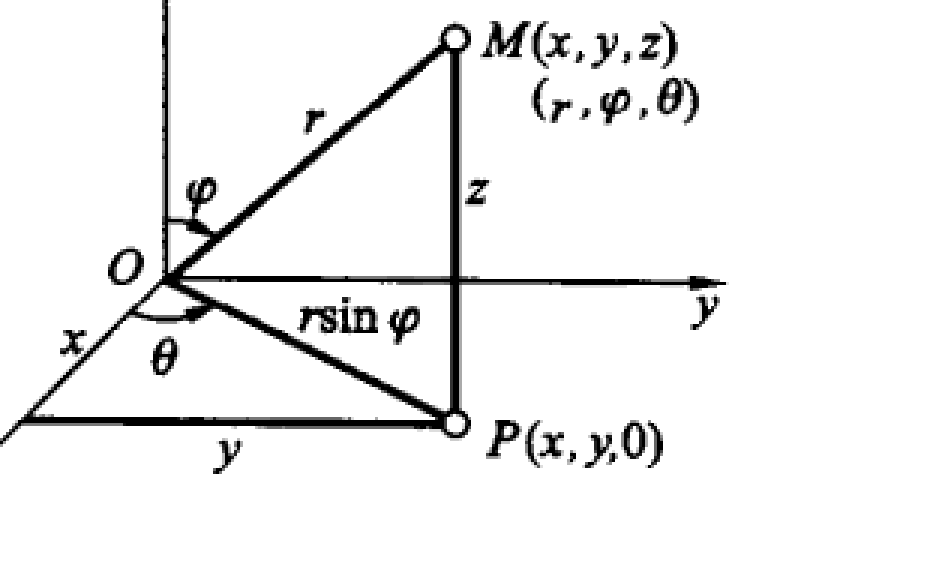
\includegraphics[width=0.34\textwidth]{work/figures/fig20-35}\caption{\relax}\label{fig:20-35}
\end{figure}

这时，体积元由半径为 $r$ 和 $r+\mathrm{d}r$ 的两块半球面，与 $Oxz$ 夹角为 $\theta$ 和 $\theta+\mathrm{d}\theta$ 的两块半平面以及与 $z$ 轴夹角为 $\varphi$ 和 $\varphi+\mathrm{d}\varphi$ 的两块锥面包围而成，其体积为（图~\ref{fig:20-36}）
\[
\mathrm{d}r\cdot r\mathrm{d}\varphi\cdot r\sin\varphi\mathrm{d}\theta=r^{2}\sin\varphi\,\mathrm{d}r\mathrm{d}\theta\mathrm{d}\varphi.
\]

\begin{figure}[htbp]
\centering
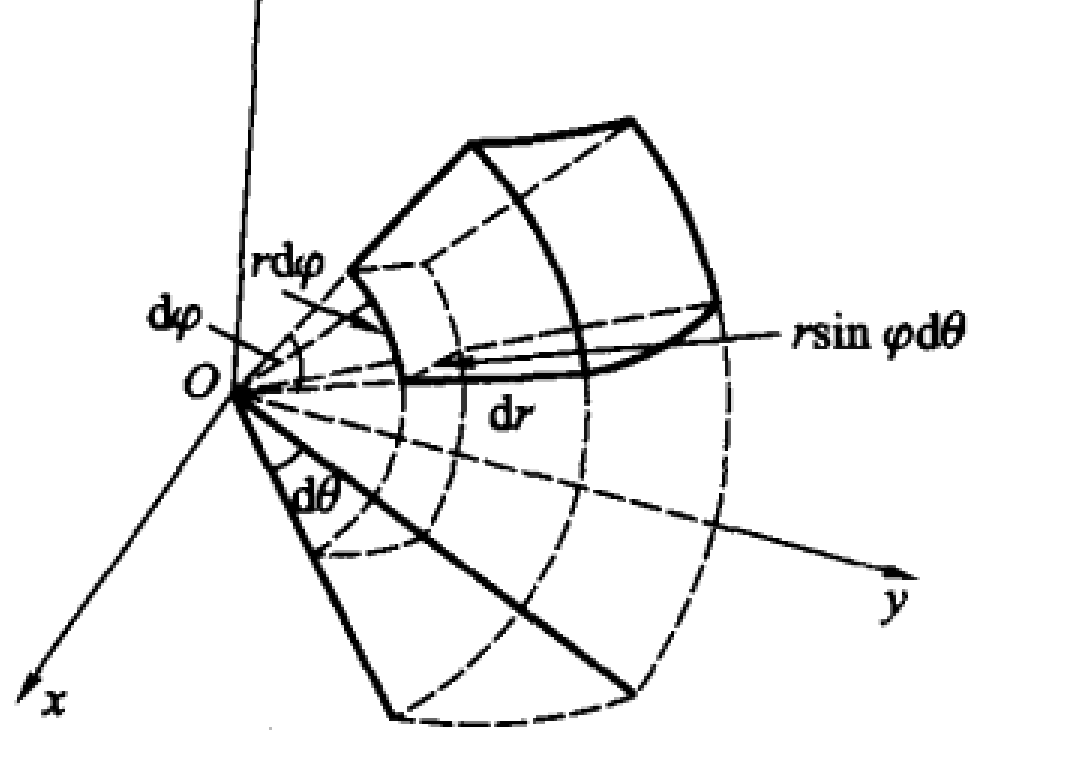
\includegraphics[width=0.38\textwidth]{work/figures/fig20-36}\caption{\relax}\label{fig:20-36}
\end{figure}

\begin{example}\label{ex:20-3-7}
求 $(x^{2}+y^{2}+z^{2})^{2}=az$ $(a>0)$ 所围区域（图~\ref{fig:20-37}）的体积．
\end{example}

\begin{proof}[解]
作球坐标变换
\[
x=r\cos\theta\sin\varphi,\quad y=r\sin\theta\sin\varphi,\quad z=r\cos\varphi.
\]
在球坐标下，曲面方程为 $r^{3}=a\cos\varphi$，区域 $V$ 可表为
\[
\left\{(r,\theta,\varphi)\mid 0\leqslant r\leqslant(a\cos\varphi)^{1/3},0\leqslant\varphi\leqslant\frac{\pi}{2},0\leqslant\theta\leqslant 2\pi\right\}.
\]

\begin{figure}[htbp]
\centering
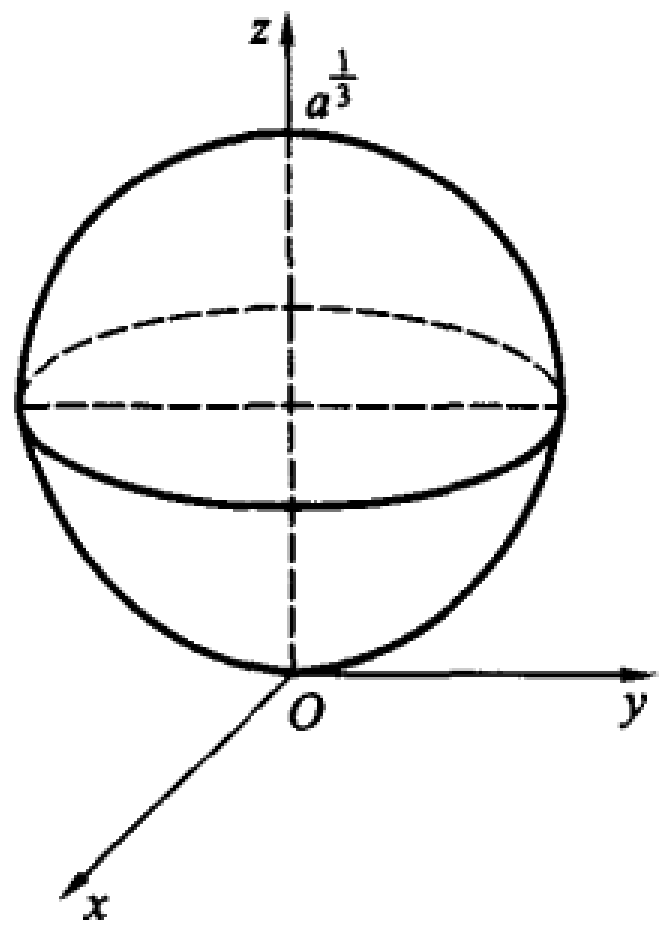
\includegraphics[width=0.28\textwidth]{work/figures/fig20-37}\caption{\relax}\label{fig:20-37}
\end{figure}

因此
\[
\begin{aligned}
V=&\iiint_{V}\mathrm{d}x\mathrm{d}y\mathrm{d}z=\int_{0}^{2\pi}\mathrm{d}\theta\int_{0}^{\frac{\pi}{2}}\mathrm{d}\varphi\int_{0}^{(a\cos\varphi)^{\frac{1}{3}}}r^{2}\sin\varphi\,\mathrm{d}r\\
=&2\pi\int_{0}^{\frac{\pi}{2}}\sin\varphi\cdot\frac{1}{3}r^{3}\bigg|_{0}^{(a\cos\varphi)^{\frac{1}{3}}}\,\mathrm{d}\varphi\\
=&\frac{2\pi a}{3}\int_{0}^{\frac{\pi}{2}}\sin\varphi\cos\varphi\,\mathrm{d}\varphi=\frac{1}{3}\pi a.
\end{aligned}
\]
\end{proof}

\begin{example}\label{ex:20-3-8}
求曲面
\[
\left(\frac{x^{2}}{a^{2}}+\frac{y^{2}}{b^{2}}+\frac{z^{2}}{c^{2}}\right)^{2}=ax\quad(a,b,c>0)
\]
所围区域的体积．
\end{example}

\begin{proof}[解]
作广义球坐标变换
\[
\begin{cases}
y=br\cos\theta\sin\varphi,\\
z=cr\sin\theta\sin\varphi,\\
x=ar\cos\varphi.
\end{cases}
\]
在变换下，曲面方程化为 $r^{3}=a^{2}\cos\varphi$．因此所围区域可表为
\[
\left\{(r,\theta,\varphi)\mid 0\leqslant\theta\leqslant 2\pi,0\leqslant\varphi\leqslant\frac{\pi}{2},0\leqslant r\leqslant(a^{2}\cos\varphi)^{\frac{1}{3}}\right\}.
\]
因为
\[
\frac{\partial(y,z,x)}{\partial(r,\theta,\varphi)}=-abcr^{2}\sin\varphi,
\]
所以
\[
V=\iiint_{V}\mathrm{d}x\mathrm{d}y\mathrm{d}z=\int_{0}^{2\pi}\mathrm{d}\theta\int_{0}^{\frac{\pi}{2}}\mathrm{d}\varphi\int_{0}^{(a^{2}\cos\varphi)^{\frac{1}{3}}}abcr^{2}\sin\varphi\,\mathrm{d}r,
\]
由上例结果便得
\[
V=\frac{1}{3}\pi a^{3}bc.
\]
\end{proof}

\begin{xiti}
\item 用极坐标变换将 $\displaystyle\iint_{D}f(x,y)\,\mathrm{d}x\,\mathrm{d}y$ 化为累次积分：
\begin{ziti}
\item $D$：半圆 $x^{2}+y^{2}\leqslant a^{2}$，$y\geqslant 0$；
\item $D$：半环 $a^{2}\leqslant x^{2}+y^{2}\leqslant b^{2}$，$x\geqslant 0$；
\item $D$：圆 $x^{2}+y^{2}\leqslant ay$ $(a>0)$；
\item $D$：正方形 $0\leqslant x\leqslant a$，$0\leqslant y\leqslant a$．
\end{ziti}
\item 用极坐标变换计算下列二重积分：
\begin{ziti}
\item $\displaystyle\iint_{D}\sin\sqrt{x^{2}+y^{2}}\,\mathrm{d}x\,\mathrm{d}y$，$D$：$\pi^{2}\leqslant x^{2}+y^{2}\leqslant 4\pi^{2}$；
\item $\displaystyle\iint_{D}(x+y)\,\mathrm{d}x\,\mathrm{d}y$，$D$ 是圆 $x^{2}+y^{2}\leqslant x+y$ 的内部；
\item $\displaystyle\iint_{D}(x^{2}+y^{2})\,\mathrm{d}x\mathrm{d}y$，$D$ 由双纽线 $(x^{2}+y^{2})^{2}=a^{2}(x^{2}-y^{2})$ $(x\geqslant 0)$ 围成；
\item $\displaystyle\iint_{D}x\,\mathrm{d}x\,\mathrm{d}y$，$D$ 由阿基米德螺线 $r=\theta$ 在 $\theta\in[0,\pi]$ 的一段和半射线 $\theta=\pi$ 围成；
\item $\displaystyle\iint_{D}xy\,\mathrm{d}x\,\mathrm{d}y$，$D$ 由对数螺线 $r=\mathrm{e}^{\theta}$ 在 $\theta\in\left[0,\dfrac{\pi}{2}\right]$ 的一段和半射线 $\theta=0$，$\theta=\dfrac{\pi}{2}$ 围成．
\end{ziti}
\item 在下列积分中引入新变量 $u$，$v$，将它们化为累次积分：
\begin{ziti}
\item $\displaystyle\int_{0}^{2}\mathrm{d}x\int_{1-x}^{2-x}f(x,y)\,\mathrm{d}y$，若 $u=x+y$，$v=x-y$；
\item $\displaystyle\int_{a}^{b}\mathrm{d}x\int_{\alpha x}^{\beta x}f(x,y)\,\mathrm{d}y$ $\left(0<a<b,0<\alpha<\beta\right)$，若 $u=x$，$v=\dfrac{y}{x}$；
\item $\displaystyle\iint_{D}f(x,y)\,\mathrm{d}x\mathrm{d}y$，其中 $D=\left\{(x,y)\mid\sqrt{x}+\sqrt{y}\leqslant\sqrt{a},x\geqslant 0,y\geqslant 0\right\}$，若 $x=u\cos^{4}v$，$y=u\sin^{4}v$；
\item $\displaystyle\iint_{D}f(x,y)\,\mathrm{d}x\mathrm{d}y$，其中 $D=\left\{(x,y)\mid x+y\leqslant a,x\geqslant 0,y\geqslant 0\right\}$ $(a>0)$，若 $x+y=u$，$y=uv$．
\end{ziti}
\item 作适当的变量代换，求下列积分：
\begin{ziti}
\item $\displaystyle\iint_{D}(x^{2}+y^{2})\,\mathrm{d}x\mathrm{d}y$，$D$ 是由 $x^{4}+y^{4}=1$ 围成的区域；
\item $\displaystyle\iint_{D}(x+y)\,\mathrm{d}x\,\mathrm{d}y$，$D$ 由 $y=4x^{2}$，$y=9x^{2}$，$x=4y^{2}$，$x=9y^{2}$ 围成；
\item $\displaystyle\iint_{D}xy\,\mathrm{d}x\,\mathrm{d}y$，$D$ 由 $xy=2$，$xy=4$，$y=x$，$y=2x$ 围成．
\end{ziti}
\item 利用二重积分求由下列曲面围成的立体的体积：
\begin{ziti}
\item $z=xy$，$x^{2}+y^{2}=a^{2}$，$z=0$；
\item $z=\dfrac{h}{R}\sqrt{x^{2}+y^{2}}$，$z=0$，$x^{2}+y^{2}=R^{2}$；
\item 球面 $x^{2}+y^{2}+z^{2}=a^{2}$ 与圆柱面 $x^{2}+y^{2}=ax$ $(a>0)$ 的公共部分；
\item $\dfrac{x^{2}}{a^{2}}+\dfrac{y^{2}}{b^{2}}+\dfrac{z^{2}}{c^{2}}=1$，$\dfrac{x^{2}}{a^{2}}+\dfrac{y^{2}}{b^{2}}=\dfrac{z^{2}}{c^{2}}$ $(z>0)$；
\item $z^{2}=\dfrac{x^{2}}{4}+\dfrac{y^{2}}{9}$，$2z=\dfrac{x^{2}}{4}+\dfrac{y^{2}}{9}$；
\item $z=x^{2}+y^{2}$，$z=x+y$．
\end{ziti}
\item 求曲线 $\left(\dfrac{x^{2}}{a^{2}}+\dfrac{y^{2}}{b^{2}}\right)^{2}=\dfrac{xy}{c^{2}}$ 所围的面积．
\item 用柱坐标变换计算下列三重积分：
\begin{ziti}
\item $\displaystyle\iiint_{V}(x^{2}+y^{2})^{2}\,\mathrm{d}x\mathrm{d}y\mathrm{d}z$，$V$ 由曲面 $z=x^{2}+y^{2}$，$z=4$，$z=16$ 围成；
\item $\displaystyle\iiint\limits_{V}\left(\sqrt{x^{2}+y^{2}}\right)^{3}\,\mathrm{d}x\mathrm{d}y\mathrm{d}z$，$V$ 由曲面 $x^{2}+y^{2}=9$，$x^{2}+y^{2}=16$，$z^{2}=x^{2}+y^{2}$，$z\geqslant 0$ 围成．
\end{ziti}
\item 用球坐标变换计算下列三重积分：
\begin{ziti}
\item $\displaystyle\iiint_{V}(x+y+z)\,\mathrm{d}x\,\mathrm{d}y\,\mathrm{d}z$，$V$：$x^{2}+y^{2}+z^{2}\leqslant R^{2}$；
\item $\displaystyle\iiint_{V}\left(\sqrt{x^{2}+y^{2}+z^{2}}\right)^{5}\,\mathrm{d}x\mathrm{d}y\mathrm{d}z$，$V$ 由 $x^{2}+y^{2}+z^{2}=2z$ 围成；
\item $\displaystyle\iiint_{V}x^{2}\,\mathrm{d}x\,\mathrm{d}y\,\mathrm{d}z$，$V$ 是 $x^{2}+y^{2}\leqslant z^{2}$，$x^{2}+y^{2}+z^{2}\leqslant 8$ 的公共部分．
\end{ziti}
\item 作适当的变量代换，求下列三重积分：
\begin{ziti}
\item $\displaystyle\iiint_{V}x^{2}y^{2}z\,\mathrm{d}x\,\mathrm{d}y\,\mathrm{d}z$，$V$ 由 $z=\dfrac{x^{2}+y^{2}}{a}$，$z=\dfrac{x^{2}+y^{2}}{b}$，$xy=c$，$xy=d$，$y=\alpha x$，$y=\beta x$ 围成的立体，其中 $0<a<b$，$0<c<d$，$0<\alpha<\beta$；
\item $\displaystyle\iiint_{V}x^{2}yz\,\mathrm{d}x\mathrm{d}y\mathrm{d}z$，$V$ 同（1）；
\item $\displaystyle\iiint_{V}y^{4}\,\mathrm{d}x\,\mathrm{d}y\,\mathrm{d}z$，$V$ 由 $x=az^{2}$，$x=bz^{2}$ $(z>0,0<a<b)$，$x=\alpha y$，$x=\beta y$ $(0<\alpha<\beta)$ 以及 $x=h$ $(>0)$ 围成；
\item $\displaystyle\iiint_{V}\mathrm{e}^{\sqrt{\frac{x^{2}}{a^{2}}+\frac{y^{2}}{b^{2}}+\frac{z^{2}}{c^{2}}}}\,\mathrm{d}x\mathrm{d}y\mathrm{d}z$，$V$ 由 $\dfrac{x^{2}}{a^{2}}+\dfrac{y^{2}}{b^{2}}+\dfrac{z^{2}}{c^{2}}=1$ 围成；
\item $\displaystyle\int_{0}^{1}\mathrm{d}x\int_{0}^{\sqrt{1-x^{2}}}\mathrm{d}y\int_{\sqrt{x^{2}+y^{2}}}^{\sqrt{2-x^{2}-y^{2}}}z^{2}\,\mathrm{d}z$．
\end{ziti}
\item 求下列各曲面所围立体之体积：
\begin{ziti}
\item $z=x^{2}+y^{2}$，$z=2(x^{2}+y^{2})$，$y=x$，$y=x^{2}$；
\item $\left(\dfrac{x}{a}+\dfrac{y}{b}\right)^{2}+\left(\dfrac{z}{c}\right)^{2}=1$ $\quad(x\geqslant 0,y\geqslant 0,z\geqslant 0,a>0,b>0,c>0)$．
\end{ziti}
\end{xiti}

\section{曲面面积}\label{sec:20-4}

作为二重积分的应用，本节讲述一般空间曲面面积的求法．首先碰到的问题是，什么叫空间曲面的面积？

回忆曲线的情形，在第八章 §2 中，我们曾把平面曲线的长度定义为内接折线长的极限，并把它用定积分表示出来．定义曲面面积的一种自然想法，就是模仿这个思路进行．

对于平面曲线，可以用内接折线来近似弧长，那么对空间曲面，能否用内接多面形来近似曲面面积呢？如果在曲面上任取四点，它们未必在同一平面上，因此一般不存在用平面四边形作成内接多面形．如果在曲面上任取三点，虽然三点可确定一平面，即可有平面三角形作成内接多面形，但当三角形的最大边长趋于零时，内接多面形的面积之和未必有确定的极限，即使有极限也未必与我们直观了解的面积相同．施瓦茨就曾证明：对圆柱面来说，这种内接三角形面积和的极限，依赖于三角形的高与底的比例，因而极限是不存在的（图~\ref{fig:20-38}）．因此，如果这样来定义曲面面积，则圆柱面也没有面积，这显然与常识不符．究其原因，就在于曲面的法向量与它的内接三角形的法向量可以任意地接近于垂直，即使三角形的最大边长任意小．因此这样的多面体的面积不可能作为曲面面积的近似值．

\begin{figure}[htbp]
\centering
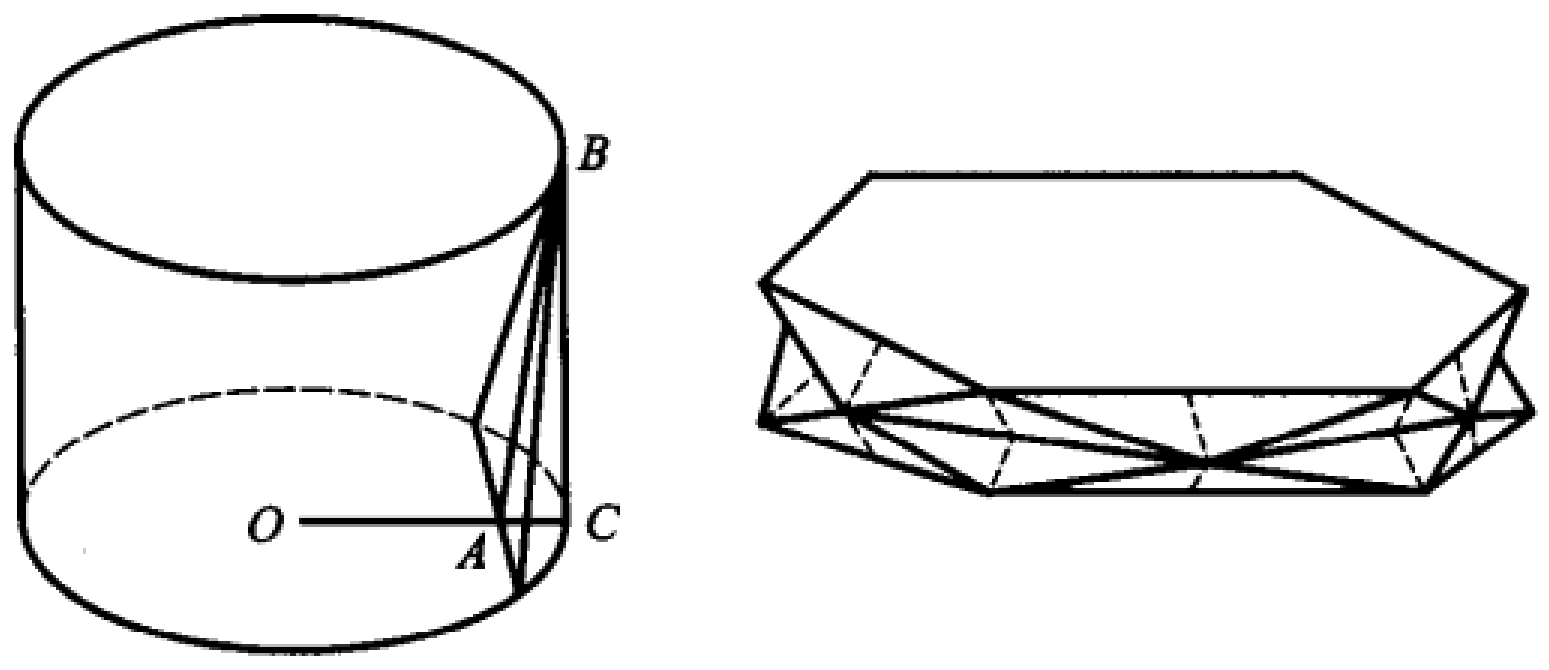
\includegraphics[width=0.55\textwidth]{work/figures/fig20-38}\caption{\relax}\label{fig:20-38}
\end{figure}

这个原因也启发我们考虑用切平面的小块面积近似小块曲面的面积，这时可以保证曲面与近似它的平面的方向保持一致．其实，在局部，曲线的弧长也是可以用切线近似的，这可以从微分三角形看出（图~\ref{fig:20-39}）：
\[
\mathrm{d}s^{2}=\mathrm{d}x^{2}+\mathrm{d}y^{2}.
\]

\begin{figure}[htbp]
\centering
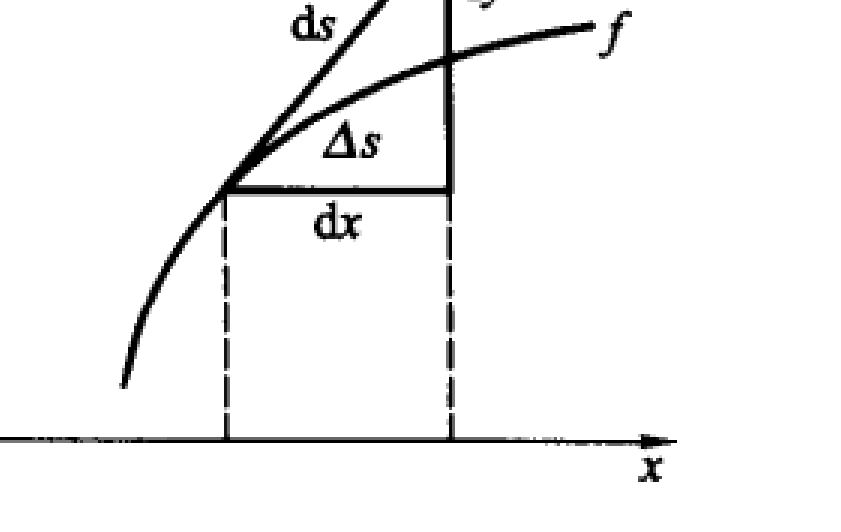
\includegraphics[width=0.32\textwidth]{work/figures/fig20-39}\caption{\relax}\label{fig:20-39}
\end{figure}

下面我们用这个办法来定义曲面的面积．先考虑曲面 $S$ 由函数
\[
z=f(x,y),\quad(x,y)\in D
\]
给出，其中 $D$ 是由逐段光滑的曲线围成．若 $f$ 具有对 $x$，$y$ 的连续偏导数，则称这曲面是\emph{光滑}的．这时曲面上任一点都存在切平面．

任意给 $D$ 一个分法 $\Delta D_{i}$ $(i=1,2,\cdots,n)$．对应于这个分法，曲面被分为 $n$ 小块 $\Delta S_{i}$，使得 $\Delta S_{i}$ 在 $Oxy$ 平面上的投影恰为 $\Delta D_{i}$．任取 $(\xi_{i},\eta_{i})\in\Delta D_{i}$，记 $\zeta_{i}=f(\xi_{i},\eta_{i})$，在曲面上的点 $(\xi_{i},\eta_{i},\zeta_{i})$ 处作切平面，并记切平面上与 $\Delta S_{i}$ 有公共投影 $\Delta D_{i}$ 的一小块为 $\Delta\sigma_{i}$，它的面积应是小块曲面 $\Delta S_{i}$ 面积（如果存在的话）的近似．记 $\lambda=\max\limits_{1\leqslant i\leqslant n}\left\{d(\Delta D_{i})\right\}$，其中 $d(\Delta D_{i})$ 是 $\Delta D_{i}$ 的直径．如果当 $\lambda\to 0$ 时，$\sum\limits_{i=1}^{n}\Delta\sigma_{i}$ 的极限存在，则称曲面 $S$ 是有面积的，且这极限便是曲面的面积：
\[
S=\lim_{\lambda\to 0}\sum_{i=1}^{n}\Delta\sigma_{i}.
\]

下面我们来计算 $\Delta\sigma_{i}$．若 $\Delta\sigma_{i}$ 的法向量 $\bm{n}_{i}$ 的方向余弦为
\[
\left(\cos\alpha_{i},\cos\beta_{i},\cos\gamma_{i}\right),
\]
则显然
\[
\Delta\sigma_{i}=\frac{\Delta D_{i}}{\left|\cos\gamma_{i}\right|}.
\]
回忆光滑曲面 $z=f(x,y)$ 在 $(\xi_{i},\eta_{i},\zeta_{i})$ 点的法向量的求法，知
\[
\bm{n}_{i}=\pm\left(f_{x}(\xi_{i},\eta_{i}),f_{y}(\xi_{i},\eta_{i}),-1\right),
\]
它与 $z$ 轴的夹角余弦为
\[
\cos\gamma_{i}=\frac{\pm 1}{\sqrt{1+f_{x}^{2}(\xi_{i},\eta_{i})+f_{y}^{2}(\xi_{i},\eta_{i})}},
\]
因此
\[
\sum_{i=1}^{n}\Delta\sigma_{i}=\sum_{i=1}^{n}\frac{\Delta D_{i}}{\left|\cos\gamma_{i}\right|}=\sum_{i=1}^{n}\sqrt{1+f_{x}^{2}(\xi_{i},\eta_{i})+f_{y}^{2}(\xi_{i},\eta_{i})}\,\Delta D_{i},
\]
上式右端恰是函数 $F(x,y)=\sqrt{1+f_{x}^{2}(x,y)+f_{y}^{2}(x,y)}$ 的黎曼和．而 $f_{x}$ 和 $f_{y}$ 在 $D$ 上连续，故 $F(x,y)$ 在 $D$ 连续．从而可积．即存在极限
\[
\begin{aligned}
S&=\lim_{\lambda\to 0}\sum_{i=1}^{n}\sqrt{1+f_{x}^{2}(\xi_{i},\eta_{i})+f_{y}^{2}(\xi_{i},\eta_{i})}\,\Delta D_{i}\\
&=\iint_{D}\sqrt{1+f_{x}^{2}(x,y)+f_{y}^{2}(x,y)}\,\mathrm{d}x\mathrm{d}y.
\end{aligned}
\]
这就是曲面 $S$ 的面积计算公式，它是 $D$ 上的一个二重积分．记
\[
\mathrm{d}S=\sqrt{1+f_{x}^{2}(x,y)+f_{y}^{2}(x,y)}\,\mathrm{d}x\mathrm{d}y=\frac{\mathrm{d}x\mathrm{d}y}{\left|\cos\gamma\right|},
\]
并称之为曲面的\emph{面积元}，它的几何意义是：曲面的面积元 $\mathrm{d}S$ 在 $Oxy$ 平面上的投影就是 $Oxy$ 平面上的面积元 $\mathrm{d}x\,\mathrm{d}y$．

\begin{example}\label{ex:20-4-1}
计算 $x^{2}+y^{2}+z^{2}=R^{2}$ 被 $x^{2}+y^{2}\leqslant Rx$ 所截出的曲面的面积．
\end{example}

\begin{proof}[解]
曲面的图形如图~\ref{fig:20-40}．由对称性，只要求出位于上半球面的那一部分，再乘 $2$ 即可．球面方程 $x^{2}+y^{2}+z^{2}=R^{2}$ 对 $x$ 求导得

\begin{figure}[htbp]
\centering
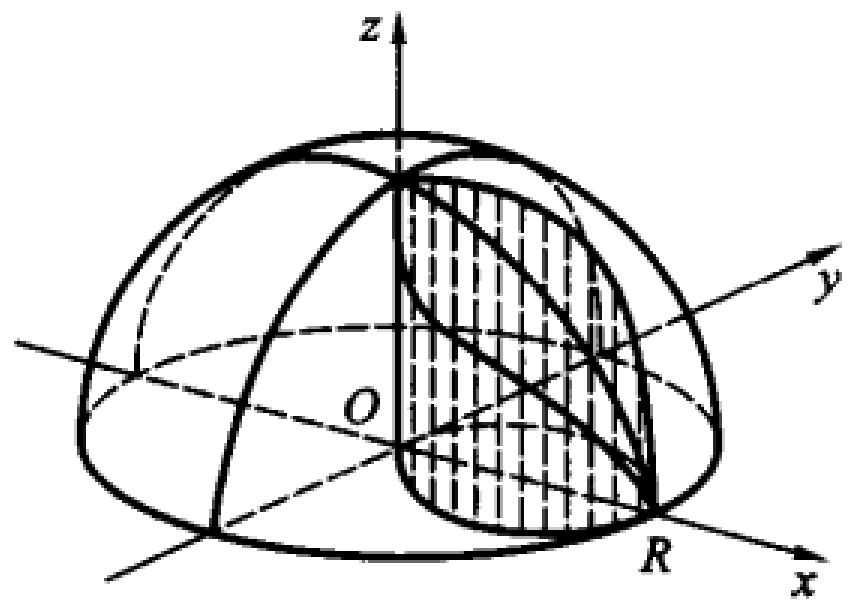
\includegraphics[width=0.34\textwidth]{work/figures/fig20-40}\caption{\relax}\label{fig:20-40}
\end{figure}
\[
2x+2z\frac{\partial z}{\partial x}=0,
\]
因此 $\dfrac{\partial z}{\partial x}=-\dfrac{x}{z}$．同理可得 $\dfrac{\partial z}{\partial y}=-\dfrac{y}{z}$．故在球面上有
\[
\begin{aligned}
&\sqrt{1+\left(\frac{\partial z}{\partial x}\right)^{2}+\left(\frac{\partial z}{\partial y}\right)^{2}}\\
=&\sqrt{1+\left(\frac{x}{z}\right)^{2}+\left(\frac{y}{z}\right)^{2}}=\frac{\sqrt{x^{2}+y^{2}+z^{2}}}{z}=\frac{R}{\sqrt{R^{2}-x^{2}-y^{2}}}.
\end{aligned}
\]
于是所求面积为
\[
S=2\iint_{D}\frac{R}{\sqrt{R^{2}-x^{2}-y^{2}}}\,\mathrm{d}x\mathrm{d}y,
\]
其中 $D$ 为 $x^{2}+y^{2}\leqslant Rx$．作极坐标变换
\[
x=r\cos\theta,\quad y=r\sin\theta,
\]
得
\[
\begin{aligned}
S&=2\iint_{D}\frac{R}{\sqrt{R^{2}-x^{2}-y^{2}}}\,\mathrm{d}x\mathrm{d}y\\
&=2R\int_{-\frac{\pi}{2}}^{\frac{\pi}{2}}\mathrm{d}\theta\int_{0}^{R\cos\theta}\frac{r\,\mathrm{d}r}{\sqrt{R^{2}-r^{2}}}\\
&=2R\int_{-\frac{\pi}{2}}^{\frac{\pi}{2}}\sqrt{R^{2}-r^{2}}\Bigg|_{R\cos\theta}^{0}\,\mathrm{d}\theta\\
&=2R\int_{-\frac{\pi}{2}}^{\frac{\pi}{2}}\left[R-R\left|\sin\theta\right|\right]\mathrm{d}\theta\\
&=4R^{2}\int_{0}^{\frac{\pi}{2}}(1-\sin\theta)\,\mathrm{d}\theta=4R^{2}\left(\frac{\pi}{2}-1\right).
\end{aligned}
\]
\end{proof}

\begin{figure}[htbp]
\centering
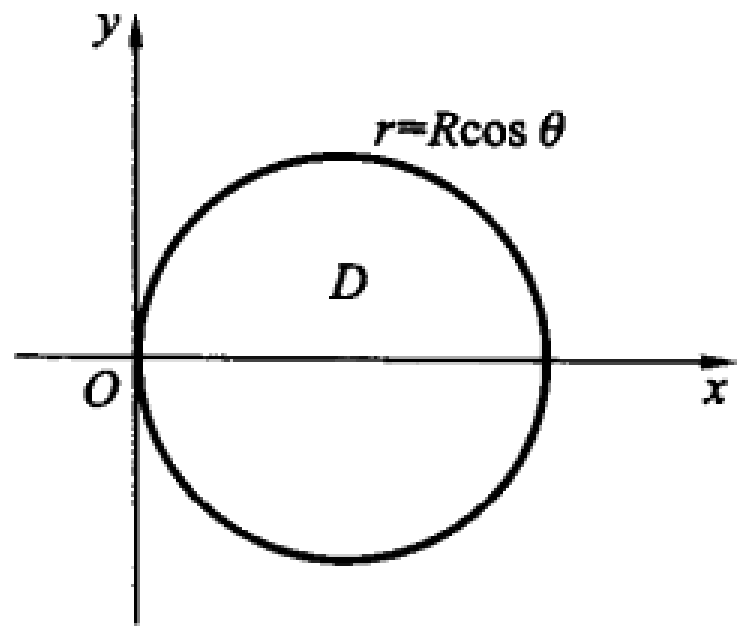
\includegraphics[width=0.34\textwidth]{work/figures/fig20-41}\caption{\relax}\label{fig:20-41}
\end{figure}

如果曲面由参数方程
\[
x=x(u,v),\quad y=y(u,v),\quad z=z(u,v),\quad(u,v)\in D
\]
给出，设函数 $x(u,v)$，$y(u,v)$，$z(u,v)$ 在 $D$ 上具有连续的一阶偏导数，且
\[
\begin{pmatrix}
\dfrac{\partial x}{\partial u} & \dfrac{\partial y}{\partial u} & \dfrac{\partial z}{\partial u}\\[6pt]
\dfrac{\partial x}{\partial v} & \dfrac{\partial y}{\partial v} & \dfrac{\partial z}{\partial v}
\end{pmatrix}
\]
在 $D$ 每一点的秩均为 $2$，则曲面是光滑曲面．曲面上每一点的法向量为
\[
\begin{aligned}
\bm{n}&=\pm\left(\frac{\partial(y,z)}{\partial(u,v)},\frac{\partial(z,x)}{\partial(u,v)},\frac{\partial(x,y)}{\partial(u,v)}\right)\\
&=\pm\begin{vmatrix}
\bm{i} & \bm{j} & \bm{k}\\
\dfrac{\partial x}{\partial u} & \dfrac{\partial y}{\partial u} & \dfrac{\partial z}{\partial u}\\[6pt]
\dfrac{\partial x}{\partial v} & \dfrac{\partial y}{\partial v} & \dfrac{\partial z}{\partial v}
\end{vmatrix}=\pm\left(\bm{r}_{u}\times\bm{r}_{v}\right),
\end{aligned}
\]
其中 $\bm{r}_{u}=\left(\dfrac{\partial x}{\partial u},\dfrac{\partial y}{\partial u},\dfrac{\partial z}{\partial u}\right)$，$\bm{r}_{v}=\left(\dfrac{\partial x}{\partial v},\dfrac{\partial y}{\partial v},\dfrac{\partial z}{\partial v}\right)$，并且 $\bm{n}$ 的三个分量中至少有一个分量不为零，为方便，记
\[
A=\frac{\partial(y,z)}{\partial(u,v)},\quad B=\frac{\partial(z,x)}{\partial(u,v)},\quad C=\frac{\partial(x,y)}{\partial(u,v)}.
\]
这样，$\bm{n}=\pm(A,B,C)$．不妨设 $C\neq 0$，这时
\[
\cos(\bm{n},z)=\frac{\pm C}{\sqrt{A^{2}+B^{2}+C^{2}}},
\]
由二重积分的变量代换公式，有
\[
\begin{aligned}
S&=\iint_{D'}\frac{\mathrm{d}x\mathrm{d}y}{\left|\cos(\bm{n},z)\right|}=\iint_{D}\frac{\left|C\right|}{\left|\cos(\bm{n},z)\right|}\,\mathrm{d}u\mathrm{d}v\\
&=\iint_{D}\sqrt{A^{2}+B^{2}+C^{2}}\,\mathrm{d}u\mathrm{d}v.
\end{aligned}
\]
由于在参数形式下，$x$，$y$，$z$ 处于同等地位，不论 $\bm{n}$ 的哪个分量不为零都可以得到同样的积分表达式
\[
S=\iint\limits_{D}\sqrt{A^{2}+B^{2}+C^{2}}\,\mathrm{d}u\mathrm{d}v,
\]
这就是在参数形式下曲面的面积公式．为便于计算，可以将积分表达式进一步变形．注意到
\[
\begin{aligned}
A^{2}+B^{2}+C^{2}&=\bm{n}\cdot\bm{n}=\left|\bm{n}\right|^{2}=\left|\bm{r}_{u}\times\bm{r}_{v}\right|^{2}\\
&=\left|\bm{r}_{u}\right|^{2}\left|\bm{r}_{v}\right|^{2}\sin^{2}(\bm{r}_{u},\bm{r}_{v})\\
&=\left|\bm{r}_{u}\right|^{2}\left|\bm{r}_{v}\right|^{2}\left(1-\cos^{2}(\bm{r}_{u},\bm{r}_{v})\right)\\
&=\left|\bm{r}_{u}\right|^{2}\left|\bm{r}_{v}\right|^{2}\left[1-\left(\frac{\bm{r}_{u}\cdot\bm{r}_{v}}{\left|\bm{r}_{u}\right|\cdot\left|\bm{r}_{v}\right|}\right)^{2}\right]\\
&=\left|\bm{r}_{u}\right|^{2}\left|\bm{r}_{v}\right|^{2}-\left(\bm{r}_{u}\cdot\bm{r}_{v}\right)^{2}.
\end{aligned}
\]
记
\[
\begin{aligned}
E&=\left|\bm{r}_{u}\right|^{2}=\left(\frac{\partial x}{\partial u}\right)^{2}+\left(\frac{\partial y}{\partial u}\right)^{2}+\left(\frac{\partial z}{\partial u}\right)^{2},\\
G&=\left|\bm{r}_{v}\right|^{2}=\left(\frac{\partial x}{\partial v}\right)^{2}+\left(\frac{\partial y}{\partial v}\right)^{2}+\left(\frac{\partial z}{\partial v}\right)^{2},\\
F&=\left(\bm{r}_{u}\cdot\bm{r}_{v}\right)=\frac{\partial x}{\partial u}\frac{\partial x}{\partial v}+\frac{\partial y}{\partial u}\frac{\partial y}{\partial v}+\frac{\partial z}{\partial u}\frac{\partial z}{\partial v}.
\end{aligned}
\]
则曲面的面积又可表为
\[
S=\iint_{D}\sqrt{EG-F^{2}}\,\mathrm{d}u\mathrm{d}v,
\]
这种形式既便于记忆，又便于计算．

\begin{example}\label{ex:20-4-2}
用参数形式求解例~\ref{ex:20-4-1}．
\end{example}

\begin{proof}[解]
球面 $x^{2}+y^{2}+z^{2}=R^{2}$ 的参数表示为
\[
\begin{aligned}
&x=R\cos\theta\sin\varphi,\quad y=R\sin\theta\sin\varphi,\quad z=R\cos\varphi,\\
&0\leqslant\theta\leqslant 2\pi,\ 0\leqslant\varphi\leqslant\pi.
\end{aligned}
\]
代入 $x^{2}+y^{2}\leqslant Rx$ 得
\[
\sin\varphi\leqslant\cos\theta,\quad-\frac{\pi}{2}\leqslant\theta\leqslant\frac{\pi}{2}.
\]
考虑第一卦限，则问题化为求球面位于
\[
D\colon 0\leqslant\varphi\leqslant\arcsin\cos\theta,\ 0\leqslant\theta\leqslant\frac{\pi}{2}
\]
部分的面积，然后再取 $4$ 倍即可．写出
\[
\begin{pmatrix}
\dfrac{\partial x}{\partial\theta} & \dfrac{\partial y}{\partial\theta} & \dfrac{\partial z}{\partial\theta}\\[6pt]
\dfrac{\partial x}{\partial\varphi} & \dfrac{\partial y}{\partial\varphi} & \dfrac{\partial z}{\partial\varphi}
\end{pmatrix}=\begin{pmatrix}
-R\sin\theta\sin\varphi & R\cos\theta\sin\varphi & 0\\
R\cos\theta\cos\varphi & R\sin\theta\cos\varphi & -R\sin\varphi
\end{pmatrix},
\]
\[
\begin{aligned}
E&=\left(R\sin\theta\sin\varphi\right)^{2}+\left(R\cos\theta\sin\varphi\right)^{2}=R^{2}\sin^{2}\varphi,\\
G&=\left(R\cos\theta\cos\varphi\right)^{2}+\left(R\sin\theta\cos\varphi\right)^{2}+\left(R\sin\varphi\right)^{2}=R^{2},\\
F&=0.
\end{aligned}
\]
故面积
\[
\begin{aligned}
S&=4\iint\limits_{D}\sqrt{EG-F^{2}}\,\mathrm{d}\theta\mathrm{d}\varphi\\
&=4\int_{0}^{\frac{\pi}{2}}\mathrm{d}\theta\int_{0}^{\arcsin\cos\theta}R^{2}\sin\varphi\,\mathrm{d}\varphi\\
&=4R^{2}\int_{0}^{\frac{\pi}{2}}(1-\sin\theta)\,\mathrm{d}\theta=4R^{2}\left(\frac{\pi}{2}-1\right),
\end{aligned}
\]
和前面计算的结果一样．
\end{proof}

\begin{xiti}
\item 求下列曲面的面积：
\begin{ziti}
\item $z=axy$ 包含在圆柱 $x^{2}+y^{2}=a^{2}$ 内的部分；
\item 锥面 $x^{2}+y^{2}=\dfrac{1}{3}z^{2}$ 与平面 $x+y+z=2a$ $(a>0)$ 所界部分的表面；
\item 锥面 $z=\sqrt{x^{2}+y^{2}}$ 被柱面 $z^{2}=2x$ 所截部分；
\item 曲面 $z=\sqrt{2xy}$ 被平面 $x+y=1$，$x=1$ 及 $y=1$ 所截下的部分．
\end{ziti}
\item 求螺旋面 $x=r\cos\varphi$，$y=r\sin\varphi$，$z=h\varphi$ $(0<r<a,\ 0<\varphi<2\pi)$ 的面积．
\item 求环面 $x=(b+a\cos\psi)\cos\varphi$，$y=(b+a\cos\psi)\sin\varphi$，$z=a\sin\psi$ $(0<a\leqslant b)$ 被两条经线 $\varphi=\varphi_{1}$，$\varphi=\varphi_{2}$ 和两条纬线 $\psi=\psi_{1}$，$\psi=\psi_{2}$ 所围成部分的面积，并求出整个环面的面积．
\end{xiti}

\section{重积分的物理应用}\label{sec:20-5}

\subsection{质心}

设 $\Omega$ 是空间的一块物体，$\rho(P)$ 是 $\Omega$ 的密度函数，它在 $\Omega$ 上连续．将 $\Omega$ 分为 $n$ 小块 $\Delta\Omega_{i}$ $(i=1,2,\cdots,n)$．由 $\rho(P)$ 的连续性，当 $\lambda=\max\limits_{1\leqslant i\leqslant n}\left\{\Delta\Omega_{i}\ \text{的直径}\right\}$ 充分小时，$\Delta\Omega_{i}$ 的质量 $\Delta m_{i}$ 有近似式
\[
\Delta m_{i}\approx\rho(P_{i})\Delta\Omega_{i},
\]
其中 $P_{i}$ 是 $\Delta\Omega_{i}$ 上的任一点．这时 $\Omega$ 可近似地视为 $n$ 个质量为 $\Delta m_{i}$ 的质点构成的质点系，质点分别位于点 $P_{i}(x_{i},y_{i},z_{i})$．因此质点系的质心坐标为
\[
\begin{aligned}
\bar{x}_{n}&=\frac{\displaystyle\sum_{i=1}^{n}x_{i}\rho(P_{i})\Delta\Omega_{i}}{\displaystyle\sum_{i=1}^{n}\rho(P_{i})\Delta\Omega_{i}},\\
\bar{y}_{n}&=\frac{\displaystyle\sum_{i=1}^{n}y_{i}\rho(P_{i})\Delta\Omega_{i}}{\displaystyle\sum_{i=1}^{n}\rho(P_{i})\Delta\Omega_{i}},\\
\bar{z}_{n}&=\frac{\displaystyle\sum_{i=1}^{n}z_{i}\rho(P_{i})\Delta\Omega_{i}}{\displaystyle\sum_{i=1}^{n}\rho(P_{i})\Delta\Omega_{i}},
\end{aligned}
\]
令 $\lambda\to 0$，由连续函数的可积性即得
\[
\begin{aligned}
\bar{x}&=\frac{\displaystyle\int_{\Omega}x\,\rho(P)\,\mathrm{d}\Omega}{\displaystyle\int_{\Omega}\rho(P)\,\mathrm{d}\Omega}=\frac{\displaystyle\int_{\Omega}x\,\mathrm{d}m}{\displaystyle\int_{\Omega}\mathrm{d}m},\\
\bar{y}&=\frac{\displaystyle\int_{\Omega}y\,\rho(P)\,\mathrm{d}\Omega}{\displaystyle\int_{\Omega}\rho(P)\,\mathrm{d}\Omega}=\frac{\displaystyle\int_{\Omega}y\,\mathrm{d}m}{\displaystyle\int_{\Omega}\mathrm{d}m},\\
\bar{z}&=\frac{\displaystyle\int_{\Omega}z\,\rho(P)\,\mathrm{d}\Omega}{\displaystyle\int_{\Omega}\rho(P)\,\mathrm{d}\Omega}=\frac{\displaystyle\int_{\Omega}z\,\mathrm{d}m}{\displaystyle\int_{\Omega}\mathrm{d}m}.
\end{aligned}
\]
这就是 $\Omega$ 的质心坐标公式，其中 $\mathrm{d}m=\rho(P)\mathrm{d}\Omega$ 是质量微元，$\displaystyle\int_{\Omega}\mathrm{d}m$ 就是 $\Omega$ 的质量．

若 $\Omega$ 是平面薄板 $D$，则 $D$ 的质心坐标为
\[
\bar{x}=\frac{\displaystyle\iint_{D}x\rho(x,y)\,\mathrm{d}x\mathrm{d}y}{\displaystyle\iint_{D}\rho(x,y)\,\mathrm{d}x\mathrm{d}y},\quad
\bar{y}=\frac{\displaystyle\iint_{D}y\rho(x,y)\,\mathrm{d}x\mathrm{d}y}{\displaystyle\iint_{D}\rho(x,y)\,\mathrm{d}x\mathrm{d}y}.
\]
若 $\Omega$ 是空间立体 $V$，则 $V$ 的质心坐标为
\[
\begin{aligned}
\bar{x}&=\frac{\displaystyle\iiint_{V}x\rho(x,y,z)\,\mathrm{d}x\mathrm{d}y\mathrm{d}z}{\displaystyle\iiint_{V}\rho(x,y,z)\,\mathrm{d}x\mathrm{d}y\mathrm{d}z},\\
\bar{y}&=\frac{\displaystyle\iiint_{V}y\rho(x,y,z)\,\mathrm{d}x\mathrm{d}y\mathrm{d}z}{\displaystyle\iiint_{V}\rho(x,y,z)\,\mathrm{d}x\mathrm{d}y\mathrm{d}z},\\
\bar{z}&=\frac{\displaystyle\iiint_{V}z\rho(x,y,z)\,\mathrm{d}x\mathrm{d}y\mathrm{d}z}{\displaystyle\iiint_{V}\rho(x,y,z)\,\mathrm{d}x\mathrm{d}y\mathrm{d}z}.
\end{aligned}
\]

\begin{example}\label{ex:20-5-1}
求球面 $x^{2}+y^{2}+z^{2}=2$ 和抛物面 $z=x^{2}+y^{2}$ 在 $z\geqslant 0$ 半空间所围立体（图~\ref{fig:20-42}）的质心，设密度 $\rho$ 为常数．
\end{example}

\begin{proof}[解]
由对称性知质心在 $z$ 轴上，即 $\bar{x}=\bar{y}=0$，而
\[
\bar{z}=\frac{\displaystyle\iiint_{V}z\,\mathrm{d}x\mathrm{d}y\mathrm{d}z}{\displaystyle\iiint_{V}\mathrm{d}x\mathrm{d}y\mathrm{d}z}.
\]

\begin{figure}[htbp]
\centering
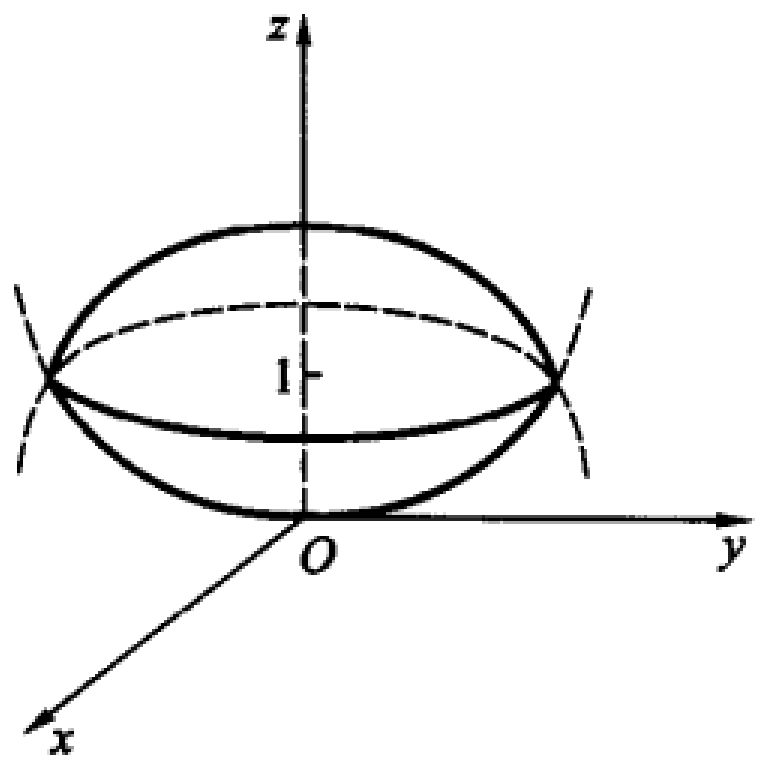
\includegraphics[width=0.28\textwidth]{work/figures/fig20-42}\caption{\relax}\label{fig:20-42}
\end{figure}

两曲面在平面 $z=1$ 上相交，因此
\[
\begin{aligned}
\iiint_{V}z\,\mathrm{d}x\mathrm{d}y\mathrm{d}z&=\int_{0}^{1}z\,\mathrm{d}z\iint_{x^{2}+y^{2}\leqslant z}\mathrm{d}x\mathrm{d}y+\int_{1}^{\sqrt{2}}z\,\mathrm{d}z\iint_{x^{2}+y^{2}\leqslant 2-z^{2}}\mathrm{d}x\mathrm{d}y\\
&=\int_{0}^{1}\pi z^{2}\,\mathrm{d}z+\int_{1}^{\sqrt{2}}\pi z(2-z^{2})\,\mathrm{d}z=\frac{7}{12}\pi.
\end{aligned}
\]
而
\[
\begin{aligned}
\iiint_{V}\mathrm{d}x\mathrm{d}y\mathrm{d}z&=\int_{0}^{1}\mathrm{d}z\iint_{x^{2}+y^{2}\leqslant z}\mathrm{d}x\mathrm{d}y+\int_{1}^{\sqrt{2}}\mathrm{d}z\iint_{x^{2}+y^{2}\leqslant 2-z^{2}}\mathrm{d}x\mathrm{d}y\\
&=\int_{0}^{1}\pi z\,\mathrm{d}z+\int_{1}^{\sqrt{2}}\pi(2-z^{2})\,\mathrm{d}z\\
&=\left(\frac{4}{3}\sqrt{2}-\frac{7}{6}\right)\pi.
\end{aligned}
\]
故
\[
\bar{z}=\frac{\dfrac{7}{12}\pi}{\left(\dfrac{4}{3}\sqrt{2}-\dfrac{7}{6}\right)\pi}=\frac{7}{2(8\sqrt{2}-7)}.
\]
\end{proof}

\subsection{转动惯量}

在第八章中我们曾经利用定积分求过某些特殊类型的平面或空间物体的转动惯量．对于一般的平面或空间物体的转动惯量，则要借助于重积分．

设 $V$ 是空间的一块物体，其密度函数 $\rho(x,y,z)$ 在 $V$ 上连续．我们来求 $V$ 对三坐标轴的转动惯量．对于 $V$ 上的任一体积元素 $\mathrm{d}V$，其质量微元为 $\mathrm{d}m=\rho(x,y,z)\mathrm{d}V$，这时 $\mathrm{d}V$ 对 $x$ 轴，$y$ 轴，$z$ 轴的转动惯量分别为
\[
\begin{aligned}
\mathrm{d}I_{x}&=\left(y^{2}+z^{2}\right)\rho(x,y,z)\mathrm{d}V=\left(y^{2}+z^{2}\right)\mathrm{d}m,\\
\mathrm{d}I_{y}&=\left(x^{2}+z^{2}\right)\rho(x,y,z)\mathrm{d}V=\left(y^{2}+z^{2}\right)\mathrm{d}m,\\
\mathrm{d}I_{z}&=\left(x^{2}+y^{2}\right)\rho(x,y,z)\mathrm{d}V=\left(x^{2}+y^{2}\right)\mathrm{d}m.
\end{aligned}
\]
由于 $V$ 对坐标轴的转动惯量就是所有质量微元对坐标轴的转动惯量的总和，这是三维连续量作用的总和，因此就是对 $\mathrm{d}I_{x}$，$\mathrm{d}I_{y}$，$\mathrm{d}I_{z}$ 求三重积分，故 $V$ 对三坐标轴的转动惯量为
\[
\begin{aligned}
I_{x}&=\iiint_{V}\left(y^{2}+z^{2}\right)\rho(x,y,z)\,\mathrm{d}x\mathrm{d}y\mathrm{d}z,\\
I_{y}&=\iiint_{V}\left(x^{2}+z^{2}\right)\rho(x,y,z)\,\mathrm{d}x\mathrm{d}y\mathrm{d}z,\\
I_{z}&=\iiint\limits_{V}\left(x^{2}+y^{2}\right)\rho(x,y,z)\,\mathrm{d}x\mathrm{d}y\mathrm{d}z.
\end{aligned}
\]
同理可得 $V$ 对坐标面的转动惯量为
\[
\begin{aligned}
I_{xy}&=\iiint_{V}z^{2}\rho(x,y,z)\,\mathrm{d}x\mathrm{d}y\mathrm{d}z,\\
I_{yz}&=\iiint_{V}x^{2}\rho(x,y,z)\,\mathrm{d}x\mathrm{d}y\mathrm{d}z,\\
I_{zx}&=\iiint_{V}y^{2}\rho(x,y,z)\,\mathrm{d}x\mathrm{d}y\mathrm{d}z.
\end{aligned}
\]

平面薄板对轴的转动惯量可类似地讨论．这里仅举例说明．

\begin{example}\label{ex:20-5-2}
求均匀圆盘 $D$：$x^{2}+y^{2}\leqslant R^{2}$ 对于其切线的转动惯量，设密度 $\rho$ 为常数．
\end{example}

\begin{proof}[解]
取切线为 $y=R$．任给面积微元 $\mathrm{d}\sigma$，它对切线 $y=R$ 的转动惯量为 $\mathrm{d}I=(R-y)^{2}\rho\,\mathrm{d}\sigma$．因此 $D$ 对 $y=R$ 的转动惯量为

\begin{figure}[htbp]
\centering
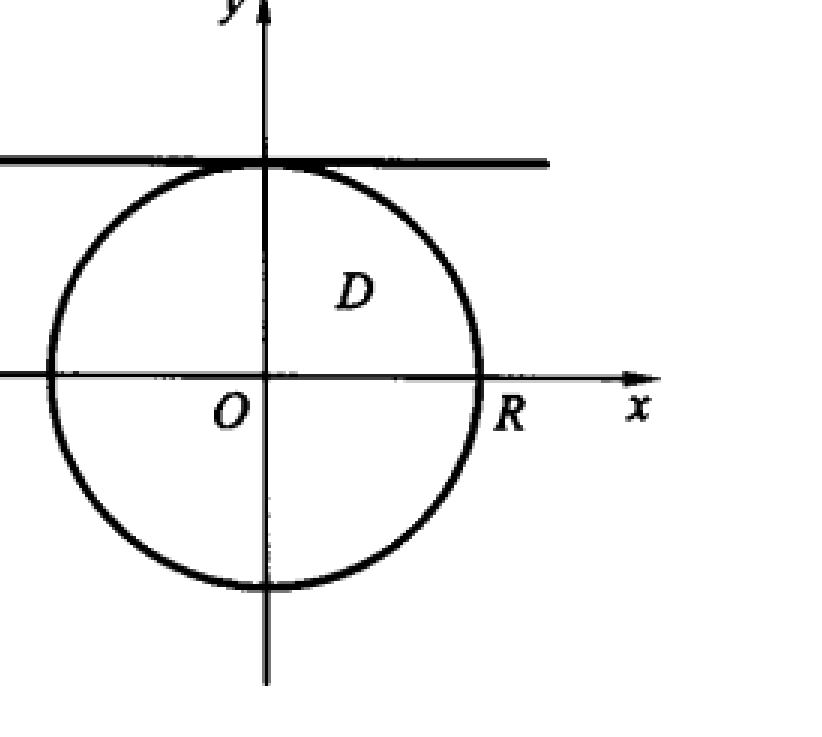
\includegraphics[width=0.28\textwidth]{work/figures/fig20-43}\caption{\relax}\label{fig:20-43}
\end{figure}
\[
\begin{aligned}
I&=\iint\limits_{D}(R-y)^{2}\rho\,\mathrm{d}\sigma\\
&=\rho\int_{0}^{2\pi}\mathrm{d}\theta\int_{0}^{R}(R-r\sin\theta)^{2}r\,\mathrm{d}r\\
&=\rho\int_{0}^{2\pi}\mathrm{d}\theta\int_{0}^{R}\left(R^{2}-2Rr\sin\theta+r^{2}\sin^{2}\theta\right)r\,\mathrm{d}r\\
&=\rho\left(2\pi R^{2}\int_{0}^{R}r\,\mathrm{d}r+\int_{0}^{2\pi}\sin^{2}\theta\,\mathrm{d}\theta\int_{0}^{R}r^{3}\,\mathrm{d}r\right)\\
&=\rho\left(\pi R^{4}+\frac{1}{4}\pi R^{4}\right)=\frac{5}{4}\rho\pi R^{4}.
\end{aligned}
\]
\end{proof}

\begin{example}\label{ex:20-5-3}
设球体的密度与球心的距离成正比，求它对于切平面的转动惯量．
\end{example}

\begin{proof}[解]
设球体的方程为 $x^{2}+y^{2}+z^{2}\leqslant R^{2}$，则密度函数为 $\rho(x,y,z)=k\sqrt{x^{2}+y^{2}+z^{2}}$，其中 $k$ 是比例常数．取切平面方程为 $z=R$，则球体对平面 $z=R$ 的转动惯量为
\[
\begin{aligned}
I&=k\iiint\limits_{V}(R-z)^{2}\sqrt{x^{2}+y^{2}+z^{2}}\,\mathrm{d}x\mathrm{d}y\mathrm{d}z\\
&=k\int_{0}^{2\pi}\mathrm{d}\theta\int_{0}^{R}\mathrm{d}r\int_{0}^{\pi}(R-r\cos\varphi)^{2}r^{3}\sin\varphi\,\mathrm{d}\varphi\\
&=2\pi k\int_{0}^{R}r^{2}\left.\frac{1}{3}(R-r\cos\varphi)^{3}\right|_{0}^{\pi}\,\mathrm{d}r\\
&=\frac{2}{3}\pi k\int_{0}^{R}r^{2}\left[(R+r)^{3}-(R-r)^{3}\right]\mathrm{d}r\\
&=\frac{4}{3}\pi k\int_{0}^{R}r^{2}\left(3R^{2}r+r^{3}\right)\mathrm{d}r=\frac{11}{9}\pi kR^{6}.
\end{aligned}
\]
\end{proof}

\begin{figure}[htbp]
\centering
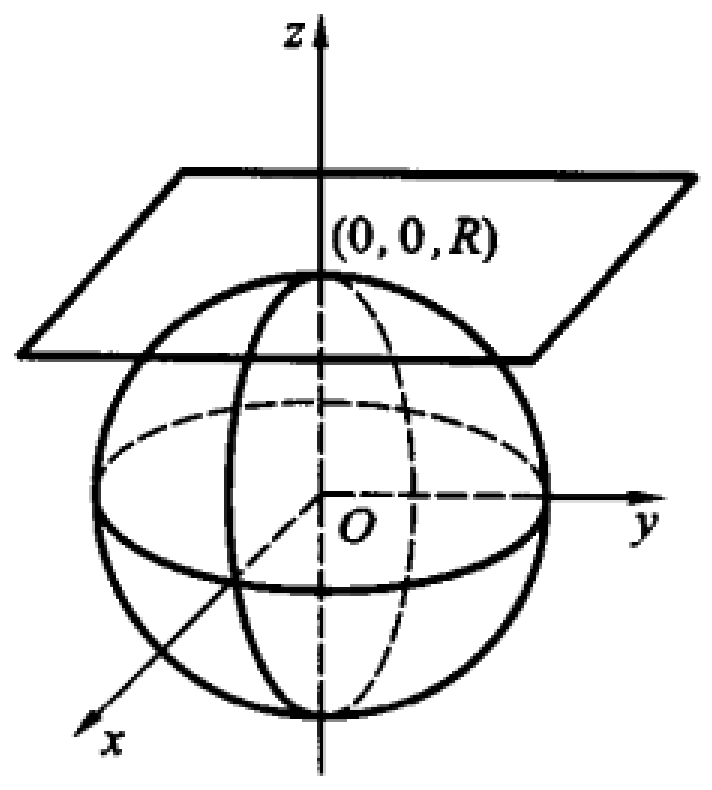
\includegraphics[width=0.26\textwidth]{work/figures/fig20-44}\caption{\relax}\label{fig:20-44}
\end{figure}

\subsection{引力}

设 $V$ 是空间的一块物体，密度函数 $\rho(x,y,z)$ 在 $V$ 上连续．求 $V$ 对 $V$ 外一点 $(x_{0},y_{0},z_{0})$ 处质量为 $1$ 的质点 $A$ 的引力 $\bm{F}$．任取 $V$ 上的质量微元 $\mathrm{d}m=\rho(x,y,z)\mathrm{d}V$．$A$ 到 $\mathrm{d}m$ 的向量为 $\bm{r}=(x-x_{0},y-y_{0},z-z_{0})$．这时 $\mathrm{d}m$ 对 $A$ 的引力为
\[
\mathrm{d}\bm{F}=\frac{k\rho(x,y,z)}{r^{3}}(x-x_{0},y-y_{0},z-z_{0})\,\mathrm{d}V,
\]
其中 $k$ 是引力常数，$r=\sqrt{(x-x_{0})^{2}+(y-y_{0})^{2}+(z-z_{0})^{2}}$．对 $V$ 求和，便得 $\bm{F}$ 在三坐标轴上的投影分别为
\[
\begin{aligned}
F_{x}&=\iiint\limits_{V}k\frac{x-x_{0}}{r^{3}}\rho(x,y,z)\,\mathrm{d}x\mathrm{d}y\mathrm{d}z,\\
F_{y}&=\iiint\limits_{V}k\frac{y-y_{0}}{r^{3}}\rho(x,y,z)\,\mathrm{d}x\mathrm{d}y\mathrm{d}z,\\
F_{z}&=\iiint\limits_{V}k\frac{z-z_{0}}{r^{3}}\rho(x,y,z)\,\mathrm{d}x\mathrm{d}y\mathrm{d}z.
\end{aligned}
\]
而 $\bm{F}=F_{x}\,\bm{i}+F_{y}\,\bm{j}+F_{z}\,\bm{k}$．

\begin{figure}[htbp]
\centering
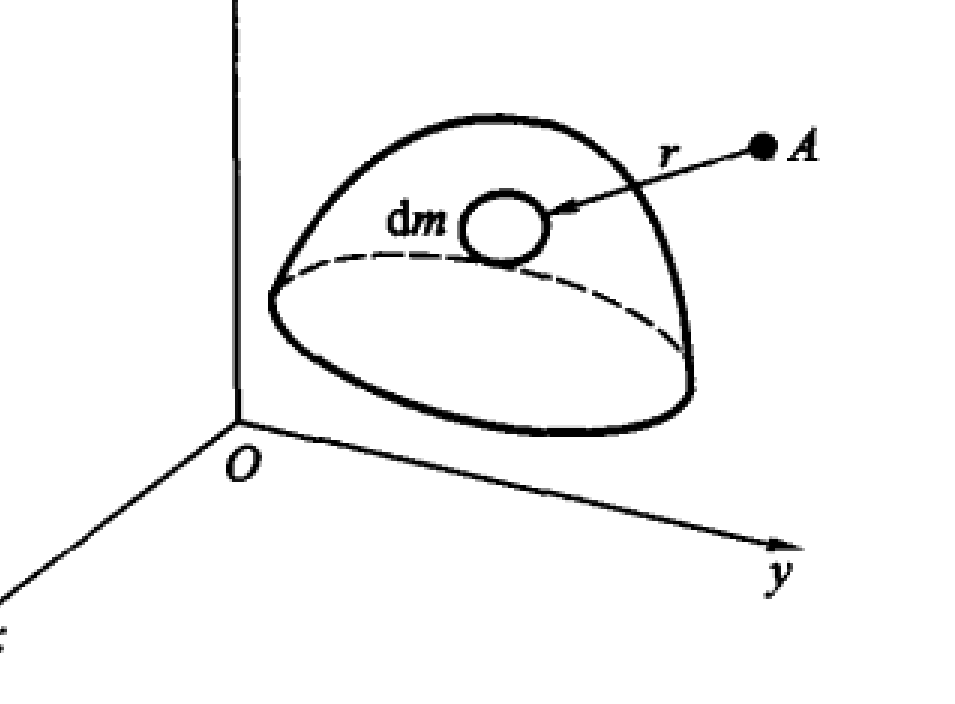
\includegraphics[width=0.32\textwidth]{work/figures/fig20-45}\caption{\relax}\label{fig:20-45}
\end{figure}

\begin{example}\label{ex:20-5-4}
求均匀球体 $x^{2}+y^{2}+z^{2}\leqslant R^{2}$ 对球外一点质量为 $1$ 的质点 $A$ 的引力．
\end{example}

\begin{proof}[解]
设球体的密度为常数 $\rho$，不妨设质点 $A$ 位于 $z$ 轴 $(0,0,h)$ 处 $(h>R)$．由对称性知 $F_{x}=F_{y}=0$．
\[
F_{z}=k\rho\iiint_{V}\frac{z-h}{\left[x^{2}+y^{2}+(z-h)^{2}\right]^{\frac{3}{2}}}\,\mathrm{d}x\mathrm{d}y\mathrm{d}z.
\]
作柱坐标变换，得
\[
\begin{aligned}
F_{z}&=k\rho\int_{0}^{2\pi}\mathrm{d}\theta\int_{-R}^{R}(z-h)\,\mathrm{d}z\int_{0}^{\sqrt{R^{2}-z^{2}}}\frac{r\,\mathrm{d}r}{\left[r^{2}+(z-h)^{2}\right]^{\frac{3}{2}}}\\
&=2\pi k\rho\int_{-R}^{R}\left(-1-\frac{z-h}{\sqrt{R^{2}+h^{2}-2hz}}\right)\mathrm{d}z\\
&=-\frac{4}{3h^{2}}\pi k\rho R^{3}.
\end{aligned}
\]
这个结果表明球体对质点 $A$ 的引力等于将球体的全部质量 $\dfrac{4}{3}\pi R^{3}\rho$ 集中于球心时对质点 $A$ 的引力．
\end{proof}

\begin{xiti}
\item 求下列均匀密度的平面薄板的质心：
\begin{ziti}
\item 半椭圆 $\dfrac{x^{2}}{a^{2}}+\dfrac{y^{2}}{b^{2}}\leqslant 1$，$\quad y\geqslant 0$；
\item 高为 $h$，底分别为 $a$ 和 $b$ 的等腰梯形；
\item $r=a(1+\cos\varphi)$ $(0\leqslant\varphi\leqslant\pi)$ 所界的薄板；
\item $ay=x^{2}$，$x+y=2a$ $(a>0)$ 所界的薄板．
\end{ziti}
\item 求下列密度均匀的物体的质心：
\begin{ziti}
\item $z\leqslant 1-x^{2}-y^{2}$，$z\geqslant 0$；
\item 由坐标面及平面 $x+2y-z=1$ 所围的四面体；
\item $z=x^{2}+y^{2}$，$x+y=a$，$x=0$，$y=0$，$z=0$ 围成的立体；
\item $z^{2}=x^{2}+y^{2}$ $(z\geqslant 0)$ 和平面 $z=h$ 围成的立体；
\item 半球壳 $a^{2}\leqslant x^{2}+y^{2}+z^{2}\leqslant b^{2}$，$\quad z\geqslant 0$．
\end{ziti}
\item 求下列密度均匀的平面薄板的转动惯量：
\begin{ziti}
\item 边长为 $a$ 和 $b$，且夹角为 $\varphi$ 的平行四边形，关于底边 $b$ 的转动惯量；
\item $y=x^{2}$，$y=1$ 所围平面图形关于直线 $y=-1$ 的转动惯量．
\end{ziti}
\item 求由下列曲面所界均匀体的转动惯量：
\begin{ziti}
\item $z=x^{2}+y^{2}$，$x+y=\pm 1$，$x-y=\pm 1$，$z=0$ 关于 $z$ 轴的转动惯量；
\item 长方体关于它的一棱的转动惯量；
\item 圆筒 $a^{2}\leqslant x^{2}+y^{2}\leqslant b^{2}$，$-h\leqslant z\leqslant h$ 关于 $x$ 轴和 $z$ 轴的转动惯量．
\end{ziti}
\item 设球体 $x^{2}+y^{2}+z^{2}\leqslant 2x$ 上各点的密度等于该点到坐标原点的距离，求这球的质量．
\item 求均匀薄片 $x^{2}+y^{2}\leqslant R^{2}$，$z=0$ 对 $z$ 轴上一点 $(0,0,c)$ $(c>0)$ 处单位质点的引力．
\item 求均匀柱体 $x^{2}+y^{2}\leqslant a^{2}$，$0\leqslant z\leqslant h$ 对于 $(0,0,c)$ $(c>h)$ 处单位质点的引力．
\end{xiti}



\chapter{曲线积分与曲面积分}

积分实际上是求连续量作用的总和．当连续量定义在直线段时，这是定积分；当连续量定义在平面的区域时，这是二重积分；当连续量定义在空间的立体时，这是三重积分．自然连续量还可以定义在空间曲线或空间曲面上，这就分别引导到曲线积分和曲面积分．定积分的积分线段是有向的，重积分的积分区域是无向的，细心的读者应看到两者的区别．定义域是无向的积分称为第一型的，定义域是有向的积分称为第二型的．因此曲线积分和曲面积分有第一型和第二型之区别，这是读者要特别注意的．

\section{第一型曲线积分与曲面积分}

上一章中，我们从求平面薄板的质量引出了二重积分，从求空间物体的质量引出了三重积分．在这里，我们将从求曲线段的质量引出第一型曲线积分，而类似地从求曲面块的质量引出第一型曲面积分．

\subsection{第一型曲线积分}

我们的问题是，设有空间的曲线段 $L$，其上每点有线密度，如何求其质量，为简单起见，设空间曲线段 $L$ 是可求长的，其端点为 $A$、$B$．又设密度函数 $f(x,y,z)$ 在曲线 $L$ 上连续，我们来求这曲线段 $L$ 的质量．

从 $A$ 至 $B$ 依次插入分点 $A=A_{0}$，$A_{1},\cdots,A_{n}=B$，它将曲线段 $L$ 分成 $n$ 小段．记第 $i$ 段弧长为 $\Delta s_{i}$ $(i=1,2,\cdots,n)$．

\begin{figure}[htbp]
\centering
\begin{tikzpicture}[scale=1]
\draw[thick] (0,0) .. controls (1.2,1.4) and (2.6,1.8) .. (4.2,1.2);
\foreach \p/\lab in {(0,0)/$A=A_{0}$,(0.55,0.62)/$A_{1}$,(1.25,1.09)/$A_{2}$,(2.5,1.42)/$A_{i-1}$,(3.2,1.38)/$A_{i}$,(3.75,1.3)/$\cdots$,(4.2,1.2)/$B=A_{n}$}{
  \fill \p circle (1.2pt);
}
\node[below left] at (0,0) {$A=A_{0}$};
\node[above left] at (0.55,0.62) {$A_{1}$};
\node[above] at (1.25,1.09) {$A_{2}$};
\node[above] at (2.5,1.42) {$A_{i-1}$};
\node[above] at (3.2,1.38) {$A_{i}$};
\node[right] at (3.75,1.28) {$\cdots$};
\node[above right] at (4.2,1.2) {$B=A_{n}$};
\node[below right] at (2.2,0.9) {$L$};
\end{tikzpicture}\caption{\relax}\label{fig:21-1}
\end{figure}

在第 $i$ 弧段上任取一点 $(\xi_{i},\eta_{i},\zeta_{i})$，则第 $i$ 弧段的质量近似于 $f(\xi_{i},\eta_{i},\zeta_{i})\Delta s_{i}$，从而 $L$ 的质量就近似于
\[
\sum_{i=1}^{n}f(\xi_{i},\eta_{i},\zeta_{i})\Delta s_{i}.
\]
当 $\lambda=\max\limits_{1\leqslant i\leqslant n}\{\Delta s_{i}\}\to0$ 时，上述和式的极限就是 $L$ 的质量
\[
M=\lim_{\lambda\to0}\sum_{i=0}^{n}f(\xi_{i},\eta_{i},\zeta_{i})\Delta s_{i}.
\]
这种定义在曲线段 $L$ 上的和式的极限，就称为 $f(x,y,z)$ 在 $L$ 的第一型曲线积分．

一般地有下述定义．

\begin{definition}\label{def:21-1}
设 $L$ 是空间可求长的曲线段，$f(x,y,z)$ 定义在 $L$ 上．$L$ 的两端点为 $A$，$B$．依次用分点 $A=A_{0},A_{1},\cdots,A_{n}=B$ 将 $L$ 分成 $n$ 小段，每小段的弧长记为 $\Delta s_{i}$，不妨将第 $i$ 小段弧也记为 $\Delta s_{i}$．任取 $(\xi_{i},\eta_{i},\zeta_{i})\in\Delta s_{i}$，作和式
\[
\sum_{i=1}^{n}f(\xi_{i},\eta_{i},\zeta_{i})\Delta s_{i}.
\]
若当 $\lambda=\max\limits_{1\leqslant i\leqslant n}\{\Delta s_{i}\}\to0$ 时上述和式极限存在，则称此极限为 $f(x,y,z)$ 在曲线 $L$ 上的\emph{第一型曲线积分}，记为
\[
\int_{L}f(x,y,z)\,\mathrm{d}s.
\]
总起来说，就是
\[
\int_{L}f(x,y,z)\,\mathrm{d}s=\lim_{\lambda\to0}\sum_{i=1}^{n}f(\xi_{i},\eta_{i},\zeta_{i})\Delta s_{i}.
\]
\end{definition}

\begin{theorem}\label{thm:21-1}
设 $L$ 是光滑曲线
\[
x=x(t),\quad y=y(t),\quad z=z(t),\quad\alpha\leqslant t\leqslant\beta,
\]
$f(x,y,z)$ 在 $L$ 上连续，则 $f(x,y,z)$ 在 $L$ 上的第一型曲线积分存在，且
\[
\begin{aligned}
&\int_{L}f(x,y,z)\,\mathrm{d}s\\
={}&\int_{\alpha}^{\beta}f(x(t),y(t),z(t))\sqrt{x^{\prime2}(t)+y^{\prime2}(t)+z^{\prime2}(t)}\,\mathrm{d}t.
\end{aligned}
\]
\end{theorem}

\begin{proof}
（1）设 $L$ 的参数方程中的参数 $t$ 是从一端点 $A$ 到曲线上的点 $(x,y,z)$ 的弧长 $s$．这时，方程化为
\[
\begin{cases}
x=x(s),\\
y=y(s),\\
z=z(s),
\end{cases}
\quad 0\leqslant s\leqslant l,
\]
这就是曲线的本性方程．因此曲线上的分点 $A=A_{0},A_{1},\cdots,A_{n}=B$ 对应于 $[0,l]$ 的分法：$0=s_{0}<s_{1}<\cdots<s_{n}=l$．$\Delta s_{i}=s_{i}-s_{i-1}$ 既表示第 $i$ 段的弧长，也表示曲线段本身．对任意 $(\xi_{i},\eta_{i},\zeta_{i})\in\Delta s_{i}$，存在 $s_{i}^{*}\in\Delta s_{i}$，使得
\[
(\xi_{i},\eta_{i},\zeta_{i})=(x(s_{i}^{*}),y(s_{i}^{*}),z(s_{i}^{*})).
\]
因此
\[
\begin{aligned}
&\sum_{i=1}^{n}f(\xi_{i},\eta_{i},\zeta_{i})\Delta s_{i}\\
={}&\sum_{i=1}^{n}f(x(s_{i}^{*}),y(s_{i}^{*}),z(s_{i}^{*}))\Delta s_{i},
\end{aligned}
\]
它是 $f(x(s),y(s),z(s))$ 在 $[0,l]$ 的黎曼和．由于 $f(x(s),y(s),z(s))$ 在 $[0,l]$ 连续，从而可积，故有
\[
\int_{0}^{l}f(x(s),y(s),z(s))\,\mathrm{d}s=\lim_{\lambda\to0}\sum_{i=1}^{n}f(\xi_{i},\eta_{i},\zeta_{i})\Delta s_{i}.
\]
由定义~\ref{def:21-1} 即得 $f(x,y,z)$ 在 $L$ 上的第一型曲线积分存在，且
\[
\int_{L}f(x,y,z)\,\mathrm{d}s=\int_{0}^{l}f(x(s),y(s),z(s))\,\mathrm{d}s.
\]
注意当参数 $s$ 是弧长参数时，$x^{\prime2}(s)+y^{\prime2}(s)+z^{\prime2}(s)=1$，因此公式成立．

（2）设 $t$ 是任意参数．回忆本性方程的求法，对 $\widehat{AB}$ 上的任一点 $P(x(t),y(t),z(t))$，求出 $\widehat{AP}$ 的弧长
\[
s(t)=\int_{\alpha}^{t}\sqrt{x^{\prime2}(\tau)+y^{\prime2}(\tau)+z^{\prime2}(\tau)}\,\mathrm{d}\tau,\quad t\in[\alpha,\beta].
\]
由于
\[
\frac{\mathrm{d}s}{\mathrm{d}t}=\sqrt{x^{\prime2}(t)+y^{\prime2}(t)+z^{\prime2}(t)}>0,
\]
根据反函数存在定理知，函数 $s(t)$ 有反函数 $t=t(s)$，它在 $[0,l]$ 上连续可微，且 $t=\alpha$ 对应于 $s=0$，$t=\beta$ 对应于 $s=l$．这时
\[
\begin{cases}
x=x(t(s)),\\
y=y(t(s)),\\
z=z(t(s)),
\end{cases}
\quad 0\leqslant s\leqslant l
\]
是 $L$ 的本性方程．由（1）已证得
\[
\int_{L}f(x,y,z)\,\mathrm{d}s=\int_{0}^{l}f(x(t(s)),y(t(s)),z(t(s)))\,\mathrm{d}s.
\]
在等式右边作定积分的变量代换 $s=s(t)$，得
\[
\begin{aligned}
&\int_{L}f(x,y,z)\,\mathrm{d}s\\
={}&\int_{\alpha}^{\beta}f(x(t),y(t),z(t))\sqrt{x^{\prime2}(t)+y^{\prime2}(t)+z^{\prime2}(t)}\,\mathrm{d}t.
\end{aligned}
\]
公式得证．定理~\ref{thm:21-1} 证完．
\end{proof}

定理~\ref{thm:21-1} 把第一型曲线积分化成了定积分，从而给出了第一型曲线积分的计算方法．

\begin{sloppypar}
其实，这公式是很容易记忆的．它指出，在曲线积分
\[
\int_{L}f(x,y,z)\,\mathrm{d}s
\]
中，把 $L$ 的参数方程 $x=x(t)$，$y=y(t)$，$z=z(t)$ 代进去，再把弧微分 $\mathrm{d}s=\sqrt{x^{\prime2}(t)+y^{\prime2}(t)+z^{\prime2}(t)}\,\mathrm{d}t$ 也代进去，积分限 $t=\alpha$ 与 $t=\beta$，是对应于 $L$ 两个端点的参数．要特别注意的是，积分限永远是从小到大．这是因为，线积分定义中的 $\Delta s_{i}$ 是真正的弧长，永远是正的．由此可见，第一型曲线积分同 $L$ 的方向无关．也就是说，如果 $L$ 的两个端点是 $A$ 与 $B$，则 $f(x,y,z)$ 在 $L$ 的第一型曲线积分由 $A$ 积到 $B$ 等于由 $B$ 积到 $A$，可以把这写成
\[
\int_{\widehat{AB}}f(x,y,z)\,\mathrm{d}s=\int_{\widehat{BA}}f(x,y,z)\,\mathrm{d}s.
\]
因为由定理~\ref{thm:21-1}，它们都化成同一个定积分．
\end{sloppypar}

当 $L$ 是平面曲线且用 $y=\varphi(x)$，$a\leqslant x\leqslant b$ 给出时，公式化为
\[
\int_{L}f(x,y)\,\mathrm{d}s=\int_{a}^{b}f(x,\varphi(x))\sqrt{1+\varphi^{\prime2}(x)}\,\mathrm{d}x.
\]
显然，当 $f(x,y,z)=1$ 时，定理~\ref{thm:21-1} 的公式化为
\[
\int_{L}\mathrm{d}s=\int_{\alpha}^{\beta}\sqrt{x^{\prime2}(t)+y^{\prime2}(t)+z^{\prime2}(t)}\,\mathrm{d}s,
\]
这就是 $L$ 的弧长，与我们对曲线积分的直观理解一致．当 $f(x,y,z)$ 是 $L$ 的线密度函数时，$\displaystyle\int_{L}f(x,y,z)\,\mathrm{d}s$ 就是曲线 $L$ 的质量．定理~\ref{thm:21-1} 给出了它们的计算方法．

\begin{example}\label{ex:21-1-1}
设 $L$ 是椭圆 $\dfrac{x^{2}}{a^{2}}+\dfrac{y^{2}}{b^{2}}=1$ 在第一象限部分，求 $I=\displaystyle\int_{L}xy\,\mathrm{d}s$．
\end{example}

\begin{proof}[解法1]
用 $L$ 的参数方程
\[
x=a\cos\theta,\quad y=b\sin\theta,\quad 0\leqslant\theta\leqslant\frac{\pi}{2},
\]
则
\[
x^{\prime}=-a\sin\theta,\quad y^{\prime}=b\cos\theta,
\]
\[
\begin{aligned}
\mathrm{d}s&=\sqrt{x^{\prime2}+y^{\prime2}}\,\mathrm{d}\theta=\sqrt{a^{2}\sin^{2}\theta+b^{2}\cos^{2}\theta}\,\mathrm{d}\theta\\
&=\sqrt{\frac{a^{2}+b^{2}}{2}+\frac{b^{2}-a^{2}}{2}\cos2\theta}\,\mathrm{d}\theta.
\end{aligned}
\]
故
\[
\begin{aligned}
I&=\int_{L}xy\,\mathrm{d}s=\int_{0}^{\frac{\pi}{2}}ab\sin\theta\cos\theta\sqrt{\frac{a^{2}+b^{2}}{2}+\frac{b^{2}-a^{2}}{2}\cos2\theta}\,\mathrm{d}\theta\\
&=-\frac{ab}{4}\int_{0}^{\frac{\pi}{2}}\sqrt{\frac{a^{2}+b^{2}}{2}+\frac{b^{2}-a^{2}}{2}\cos2\theta}\,\mathrm{d}\cos2\theta\\
&=-\frac{ab}{3(b^{2}-a^{2})}\left(\frac{a^{2}+b^{2}}{2}+\frac{b^{2}-a^{2}}{2}\cos2\theta\right)^{\frac{3}{2}}\Bigg|_{0}^{\frac{\pi}{2}}\\
&=\frac{ab}{3}\frac{a^{2}+ab+b^{2}}{a+b}.
\end{aligned}
\]
\end{proof}

\begin{proof}[解法2]
用 $L$ 的直角坐标方程
\[
y=\frac{b}{a}\sqrt{a^{2}-x^{2}},\quad 0\leqslant x\leqslant a,
\]
则
\[
y^{\prime}=-\frac{bx}{a\sqrt{a^{2}-x^{2}}},
\]
\[
\mathrm{d}s=\sqrt{1+y^{\prime2}}\,\mathrm{d}x=\frac{1}{a}\sqrt{\frac{a^{4}-(a^{2}-b^{2})x^{2}}{a^{2}-x^{2}}}\,\mathrm{d}x.
\]
因此
\[
\begin{aligned}
I&=\int_{L}xy\,\mathrm{d}s=\int_{0}^{a}\frac{b}{a^{2}}x\sqrt{a^{4}-(a^{2}-b^{2})x^{2}}\,\mathrm{d}x\\
&=\frac{b}{3a^{2}(b^{2}-a^{2})}\left[a^{4}-(a^{2}-b^{2})x^{2}\right]^{\frac{3}{2}}\bigg|_{0}^{a}\\
&=\frac{ab}{3}\frac{a^{2}+ab+b^{2}}{a+b}.
\end{aligned}
\]
\end{proof}

\begin{example}\label{ex:21-1-2}
计算 $\displaystyle\int_{L}x^{2}\,\mathrm{d}s$，其中 $L$ 为球面 $x^{2}+y^{2}+z^{2}=a^{2}$ 被平面 $x+y+z=0$ 所截得的圆周．
\end{example}

\begin{proof}[解]
曲线 $L$ 是半径为 $a$、圆心在原点的圆周．但它的参数方程并不易写出．注意到 $L$ 关于 $x$，$y$，$z$ 的对称性，则有
\[
\int_{L}x^{2}\,\mathrm{d}s=\int_{L}y^{2}\,\mathrm{d}s=\int_{L}z^{2}\,\mathrm{d}s.
\]
因此
\[
\begin{aligned}
\int_{L}x^{2}\,\mathrm{d}s&=\frac{1}{3}\int_{L}(x^{2}+y^{2}+z^{2})\,\mathrm{d}s\\
&=\frac{a^{2}}{3}\int_{L}\mathrm{d}s=\frac{2}{3}\pi a^{3}.
\end{aligned}
\]
\end{proof}

对称性和几何意义是简化积分计算的常用技巧，读者应多多留意并灵活运用．

\begin{example}\label{ex:21-1-3}
试求一均匀半圆周（密度 $\rho=1$）对位于其中心的单位质点的引力．
\end{example}

\begin{proof}[解]
为计算方便，取半圆周为圆心在原点的上半圆周．设半径为 $R$，则 $x=R\cos\theta$，$y=R\sin\theta$，$(0\leqslant\theta\leqslant\pi)$．由对称性知引力 $\bm{F}$ 在 $x$ 轴上的投影 $F_{x}=0$，故只要计算 $\bm{F}$ 在 $y$ 轴上的投影 $F_{y}$．任取弧长微元 $\mathrm{d}s$，它对原点处单位质量的质点的引力为
\[
\mathrm{d}\bm{F}=\frac{k_{\rho}}{R^{2}}\mathrm{d}s\bm{r}_{0},
\]
其中 $k$ 是引力常数，$\bm{r}_{0}$ 是向径的单位向量．将 $\rho=1$，$\mathrm{d}s=R\mathrm{d}\theta$ 代进去，得 $\mathrm{d}\bm{F}$ 在 $y$ 轴上的投影为
\[
\mathrm{d}F_{y}=\frac{k}{R^{2}}\sin\theta\,\mathrm{d}s=\frac{k}{R}\sin\theta\,\mathrm{d}\theta.
\]
故 $F_{y}=\displaystyle\int_{0}^{\pi}\frac{k}{R}\sin\theta\,\mathrm{d}\theta=\frac{k}{R}\cos\theta\,\bigg|_{\pi}^{0}=\frac{2k}{R}$．
\end{proof}

\begin{figure}[htbp]
\centering
\begin{tikzpicture}[scale=0.9]
\draw[->,thick] (-2.4,0) -- (2.4,0) node[below left] {$x$};
\draw[->,thick] (0,-0.4) -- (0,2.1) node[below left] {$y$};
\draw[thick] (0,0) arc (0:180:1.8);
\draw[thick,->] (0,0) -- (40:1.8) node[midway,above left] {$R$};
\draw (0:0.55) arc (0:40:0.55) node[right,xshift=1pt] {$\theta$};
\node[below left] at (0,0) {$O$};
\node[below] at (1.8,0) {$R$};
\node[below] at (-1.8,0) {$-R$};
\node[right] at (45:1.85) {$\mathrm{d}s$};
\end{tikzpicture}\caption{\relax}\label{fig:21-2}
\end{figure}

\subsection{第一型曲面积分}

类似于第一型曲线积分，我们可以给出第一型曲面积分的定义．

\begin{definition}\label{def:21-2}
设 $S$ 是空间光滑曲面 $z=z(x,y)$，$(x,y)\in D$，$f(x,y,z)$ 是定义在 $S$ 上的函数．对于 $D$ 的任意分法 $\Delta\sigma_{i}$，相应地得到 $S$ 的分法 $\Delta S_{i}$ $(i=1,2,\cdots,n)$．任取 $(\xi_{i},\eta_{i},\zeta_{i})\in\Delta S_{i}$，记 $\lambda=\max\limits_{1\leqslant i\leqslant n}\{\Delta\sigma_{i}\ \text{的直径}\}$．若极限
\[
\lim_{\lambda\to0}\sum_{i=1}^{n}f(\xi_{i},\eta_{i},\zeta_{i})\Delta S_{i}
\]
存在，则称该极限值为 $f(x,y,z)$ 在曲面 $S$ 上的\emph{第一型曲面积分}，记为
\[
\iint_{S}f(x,y,z)\,\mathrm{d}S.
\]
\end{definition}

\begin{theorem}\label{thm:21-2}
设 $S:z=z(x,y)$，$(x,y)\in D$ 是光滑曲面，$D$ 是有界闭区域，$f(x,y,z)$ 在 $S$ 上连续，则 $f(x,y,z)$ 在曲面 $S$ 上的第一型曲面积分存在，且
\[
\begin{aligned}
&\iint_{S}f(x,y,z)\,\mathrm{d}S\\
={}&\iint_{D}f(x,y,z(x,y))\sqrt{1+z_{x}^{2}(x,y)+z_{y}^{2}(x,y)}\,\mathrm{d}x\mathrm{d}y.
\end{aligned}
\]
\end{theorem}

\begin{proof}
对于 $D$ 的任意分法 $\Delta\sigma_{i}$，相应地有 $S$ 的分法 $\Delta S_{i}$ $(i=1,2,\cdots,n)$．$\Delta S_{i}$ 的面积为
\[
\Delta S_{i}=\iint_{\Delta\sigma_{i}}\sqrt{1+z_{x}^{2}(x,y)+z_{y}^{2}(x,y)}\,\mathrm{d}x\mathrm{d}y.
\]
由二重积分的中值定理
\[
\Delta S_{i}=\sqrt{1+z_{x}^{2}(\xi_{i}^{*},\eta_{i}^{*})+z_{y}^{2}(\xi_{i}^{*},\eta_{i}^{*})}\,\Delta\sigma_{i},
\]
其中 $(\xi_{i}^{*},\eta_{i}^{*})\in\Delta\sigma_{i}$．这时曲面积分的黎曼和
\[
\begin{aligned}
\sigma&=\sum_{i=1}^{n}f(\xi_{i},\eta_{i},\zeta_{i})\Delta S_{i}\\
&=\sum_{i=1}^{n}f(\xi_{i},\eta_{i},z(\xi_{i},\eta_{i}))\sqrt{1+z_{x}^{2}(\xi_{i}^{*},\eta_{i}^{*})+z_{y}^{2}(\xi_{i}^{*},\eta_{i}^{*})}\,\Delta\sigma_{i}.
\end{aligned}
\]
令 $\lambda=\max\limits_{1\leqslant i\leqslant n}\{\Delta\sigma_{i}\ \text{的直径}\}$．我们要证明
\[
\lim_{\lambda\to0}\sigma=\iint_{D}f(x,y,z(x,y))\sqrt{1+z_{x}^{2}(x,y)+z_{y}^{2}(x,y)}\,\mathrm{d}x\mathrm{d}y.
\]
要注意的是 $\sigma$ 并不是某个函数二重积分的黎曼和，因为 $(\xi_{i},\eta_{i})$ 和 $(\xi_{i}^{*},\eta_{i}^{*})$ 可能是 $\Delta\sigma_{i}$ 中不同的两点．但这种情况我们在定积分中已多次见过．仿照定积分，记
\[
\sigma^{*}=\sum_{i=1}^{n}f(\xi_{i}^{*},\eta_{i}^{*},z(\xi_{i}^{*},\eta_{i}^{*}))\sqrt{1+z_{x}^{2}(\xi_{i}^{*},\eta_{i}^{*})+z_{y}^{2}(\xi_{i}^{*},\eta_{i}^{*})}\,\Delta\sigma_{i},
\]
则有
\[
\lim_{\lambda\to0}\sigma^{*}=\iint_{D}f(x,y,z(x,y))\sqrt{1+z_{x}^{2}(x,y)+z_{y}^{2}(x,y)}\,\mathrm{d}x\mathrm{d}y.
\]
而 $\sigma=(\sigma-\sigma^{*})+\sigma^{*}$，因此剩下只要证 $\lim\limits_{\lambda\to0}(\sigma-\sigma^{*})=0$．

因为 $\sqrt{1+z_{x}^{2}(x,y)+z_{y}^{2}(x,y)}$ 在有界闭集 $D$ 上连续，所以有最大值 $M$．因此
\[
|\sigma-\sigma^{*}|\leqslant M\sum_{i=1}^{n}\left|f(\xi_{i},\eta_{i},z(\xi_{i},\eta_{i}))-f(\xi_{i}^{*},\eta_{i}^{*},z(\xi_{i}^{*},\eta_{i}^{*}))\right|\Delta\sigma_{i}.
\]
根据 $f(x,y,z(x,y))$ 在 $D$ 上连续，从而一致连续，即对任给的 $\varepsilon>0$，存在 $\delta>0$，只要 $\lambda<\delta$（此时必有 $\Delta\sigma_{i}$ 的直径小于 $\delta$），有
\[
\left|f(\xi_{i},\eta_{i},z(\xi_{i},\eta_{i}))-f(\xi_{i}^{*},\eta_{i}^{*},z(\xi_{i}^{*},\eta_{i}^{*}))\right|<\frac{\varepsilon}{M|D|}.
\]
故
\[
|\sigma-\sigma^{*}|<\frac{\varepsilon}{|D|}\sum_{i=1}^{n}\Delta\sigma_{i}=\varepsilon.
\]
这就证明了 $\lim\limits_{\lambda\to0}(\sigma-\sigma^{*})=0$．定理~\ref{thm:21-2} 证完．
\end{proof}

公式的左端是第一型曲面积分，右端则是二重积分．二重积分是会计算了的，因此，它给出了第一型曲面积分的计算方法．在公式中取 $f(x,y,z)=1$，则有
\[
\iint_{S}\mathrm{d}S=\iint_{D}\sqrt{1+z_{x}^{2}(x,y)+z_{y}^{2}(x,y)}\,\mathrm{d}x\mathrm{d}y.
\]
这就是曲面 $S$ 的面积．它同时也表明 $\mathrm{d}S$ 就是曲面的面积元．

定理~\ref{thm:21-2} 的公式也是很易记忆的．它指出，只要把曲面方程 $z=z(x,y)$ 以及曲面面积元 $\mathrm{d}S=\sqrt{1+z_{x}^{2}+z_{y}^{2}}\,\mathrm{d}x\mathrm{d}y$ 代进曲面积分中去，积分区域就是 $S$ 在 $Oxy$ 平面的投影 $D$，便把曲面积分化成了二重积分．

当光滑曲面由参数方程
\[
x=x(u,v),\quad y=y(u,v),\quad z=z(u,v),\quad(u,v)\in D
\]
给出时，面积元为
\[
\mathrm{d}S=\sqrt{EG-F^{2}}\,\mathrm{d}u\mathrm{d}v,
\]
其中 $E=x_{u}^{2}+y_{u}^{2}+z_{u}^{2}$，$G=x_{v}^{2}+y_{v}^{2}+z_{v}^{2}$，$F=x_{u}x_{v}+y_{u}y_{v}+z_{u}z_{v}$．

因此可以设想有
\[
\iint_{S}f(x,y,z)\,\mathrm{d}S=\iint_{D}f(x(u,v),y(u,v),z(u,v))\sqrt{EG-F^{2}}\,\mathrm{d}u\mathrm{d}v.
\]
事实上，这个公式可仿照定理~\ref{thm:21-2} 加以证明，我们把它留给读者作为练习．

平面作为曲面的特殊情形，当 $S$ 是 $Oxy$ 平面上的平面块 $D$ 时，第一型曲面积分就是二重积分．事实上这时定义在 $S$ 的函数为 $f(x,y)$，$\mathrm{d}S=\mathrm{d}x\mathrm{d}y$，故
\[
\iint_{S}f(x,y)\,\mathrm{d}S=\iint_{D}f(x,y)\,\mathrm{d}x\mathrm{d}y.
\]

\begin{example}\label{ex:21-2-1}
计算曲面积分 $\displaystyle\iint_{S}\frac{\mathrm{d}S}{z}$，其中 $S$ 是球面 $x^{2}+y^{2}+z^{2}=a^{2}$ 在平面 $z=h$ $(0<h<a)$ 之上的部分（图~\ref{fig:21-3}）．
\end{example}

\begin{figure}[htbp]
\centering
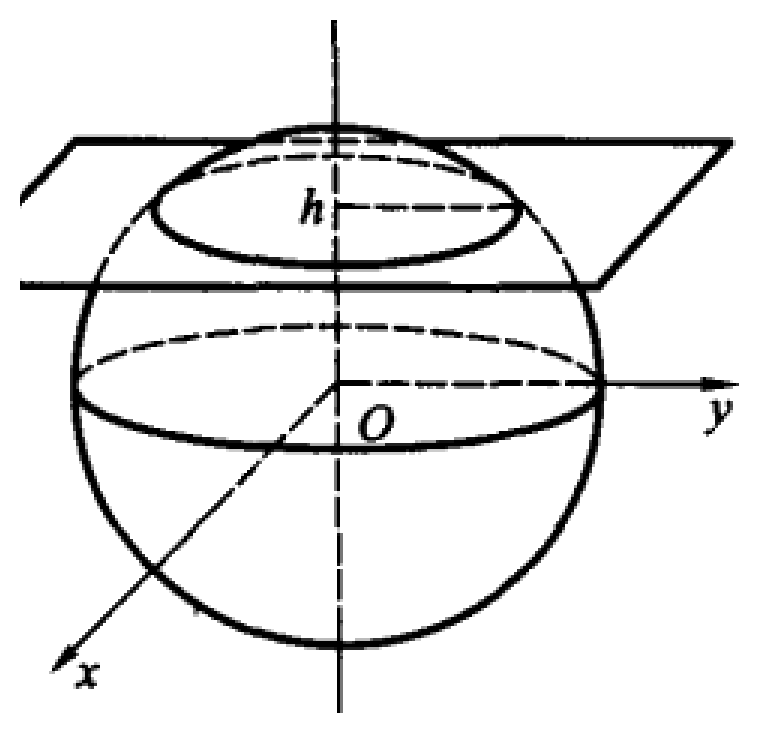
\includegraphics[width=0.42\textwidth]{work/figures/fig21-3}\caption{\relax}\label{fig:21-3}
\end{figure}

\begin{proof}[解]
曲面 $S$ 在 $Oxy$ 面上的投影区域 $D$ 为 $x^{2}+y^{2}\leqslant a^{2}-h^{2}$，而
\[
\sqrt{1+z_{x}^{2}(x,y)+z_{y}^{2}(x,y)}=\frac{a}{\sqrt{a^{2}-x^{2}-y^{2}}}.
\]
因此
\[
\begin{aligned}
\iint_{S}\frac{\mathrm{d}S}{z}&=\iint_{D}\frac{a}{a^{2}-x^{2}-y^{2}}\,\mathrm{d}x\mathrm{d}y\\
&=\int_{0}^{2\pi}\mathrm{d}\theta\int_{0}^{\sqrt{a^{2}-h^{2}}}\frac{a}{a^{2}-r^{2}}r\,\mathrm{d}r\\
&=\pi a\ln\left|a^{2}-r^{2}\right|\bigg|_{\sqrt{a^{2}-h^{2}}}^{0}\\
&=2a\pi\ln\frac{a}{h}.
\end{aligned}
\]
\end{proof}

\begin{example}\label{ex:21-2-2}
计算 $\displaystyle\iint_{S}(x+y+z)\,\mathrm{d}S$，其中 $S$ 是球面 $x^{2}+y^{2}+z^{2}=a^{2}$，$z\geqslant0$．
\end{example}

\begin{proof}[解]
本题用 $S$ 的参数方程更简便些，利用球坐标易写出 $S$ 的参数方程为
\[
\begin{cases}
x=a\cos\theta\sin\varphi,\\
y=a\sin\theta\sin\varphi,\\
z=a\cos\varphi,
\end{cases}
\quad 0\leqslant\theta\leqslant2\pi,\quad 0\leqslant\varphi\leqslant\frac{\pi}{2}.
\]
计算
\[
\begin{aligned}
\begin{pmatrix}x_{\theta}&y_{\theta}&z_{\theta}\\ x_{\varphi}&y_{\varphi}&z_{\varphi}\end{pmatrix}
&=\begin{pmatrix}-a\sin\theta\sin\varphi&a\cos\theta\sin\varphi&0\\ a\cos\theta\cos\varphi&a\sin\theta\cos\varphi&-a\sin\varphi\end{pmatrix},\\
E&=a^{2}\sin^{2}\varphi,\quad G=a^{2},\quad F=0.
\end{aligned}
\]
因此
\[
\begin{aligned}
&\iint_{S}(x+y+z)\,\mathrm{d}S\\
={}&\iint_{D}a(\cos\theta\sin\varphi+\sin\theta\sin\varphi+\cos\varphi)\sqrt{a^{4}\sin^{2}\varphi}\,\mathrm{d}\theta\mathrm{d}\varphi\\
={}&a^{3}\int_{0}^{\frac{\pi}{2}}\sin\varphi\,\mathrm{d}\varphi\int_{0}^{2\pi}(\cos\theta\sin\varphi+\sin\theta\sin\varphi+\cos\varphi)\,\mathrm{d}\theta\\
={}&2\pi a^{3}\int_{0}^{\frac{\pi}{2}}\sin\varphi\cos\varphi\,\mathrm{d}\varphi=\pi a^{3}.
\end{aligned}
\]
\end{proof}

读者不难发现此例中 $\displaystyle\iint_{S}x\,\mathrm{d}S=\iint_{S}y\,\mathrm{d}S=0$．$\iint_{S}x\,\mathrm{d}S=0$ 是因为曲面 $S$ 关于 $Oyz$ 平面对称，而被积函数是 $x$ 的奇函数．同理知 $\displaystyle\iint_{S}y\,\mathrm{d}S=0$．

\begin{example}\label{ex:21-2-3}
求均匀球壳对不在该球壳上的一单位质点 $M$ 的引力．设球壳的密度 $\rho=1$．
\end{example}

\begin{proof}[解]
为计算方便，选择质点位于 $z$ 轴上 $(0,0,h)$ 处 $(h>0)$，球壳的球心在原点，半径为 $R(R\neq h)$．

由对称性知引力 $\bm{F}$ 在 $x$ 轴和 $y$ 轴上的投影为零，故只要求 $\bm{F}$ 在 $z$ 轴上的投影 $F_{z}$．

任取面积微元 $\mathrm{d}S$，它对 $M$ 的引力为
\[
\mathrm{d}\bm{F}=\frac{k_{\rho}\,\mathrm{d}S}{r^{2}}\bm{r}_{0},
\]
其中 $r=\sqrt{x^{2}+y^{2}+(z-h)^{2}}$，$\bm{r}_{0}=\dfrac{1}{r}(x,y,z-h)$，$\rho=1$．因此 $\mathrm{d}\bm{F}$ 在 $z$ 轴上的投影为
\[
\mathrm{d}F_{z}=\frac{k(z-h)}{r^{3}}\,\mathrm{d}S.
\]
故
\[
F_{z}=\iint_{S}\frac{k(z-h)}{r^{3}}\,\mathrm{d}S.
\]
用球面的参数方程
\[
\begin{cases}
x=R\cos\theta\sin\varphi,\\
y=R\sin\theta\sin\varphi,\\
z=R\cos\varphi,
\end{cases}
\quad 0\leqslant\theta\leqslant2\pi,\qquad 0\leqslant\varphi\leqslant\pi,
\]
则
\[
\begin{aligned}
\mathrm{d}S&=\sqrt{EG-F^{2}}\,\mathrm{d}\theta\mathrm{d}\varphi=R^{2}\sin\varphi\,\mathrm{d}\theta\mathrm{d}\varphi,\\
r&=\sqrt{R^{2}+h^{2}-2Rh\cos\varphi}.
\end{aligned}
\]
从而
\[
\begin{aligned}
F_{z}&=\int_{0}^{2\pi}\mathrm{d}\theta\int_{0}^{\pi}\frac{k(R\cos\varphi-h)}{(R^{2}+h^{2}-2Rh\cos\varphi)^{\frac{3}{2}}}R^{2}\sin\varphi\,\mathrm{d}\varphi\\
&=2\pi kR^{2}\int_{0}^{\pi}\frac{R\cos\varphi-h}{(R^{2}+h^{2}-2Rh\cos\varphi)^{\frac{3}{2}}}\sin\varphi\,\mathrm{d}\varphi\\
&=\frac{\pi kR^{2}}{h}\int_{0}^{\pi}\frac{(R^{2}+h^{2}-2Rh\cos\varphi)+2h^{2}-h^{2}-R^{2}}{(R^{2}+h^{2}-2Rh\cos\varphi)^{\frac{3}{2}}}\,\mathrm{d}\cos\varphi\\
&=\frac{\pi kR^{2}}{h}\left[\int_{0}^{\pi}\frac{\mathrm{d}\cos\varphi}{(R^{2}+h^{2}-2Rh\cos\varphi)^{\frac{1}{2}}}+\int_{0}^{\pi}\frac{(h^{2}-R^{2})\,\mathrm{d}\cos\varphi}{(R^{2}+h^{2}-2Rh\cos\varphi)^{\frac{3}{2}}}\right]\\
&=\frac{\pi kR^{2}}{h}\left[\frac{1}{Rh}\sqrt{R^{2}+h^{2}-2Rh\cos\varphi}\,\Bigg|_{\pi}^{0}-\frac{h^{2}-R^{2}}{Rh}\frac{1}{\sqrt{R^{2}+h^{2}-2Rh\cos\varphi}}\,\Bigg|_{\pi}^{0}\right]\\
&=\frac{\pi kR}{h^{2}}\left[|R-h|-(R+h)-(h^{2}-R^{2})\left(\frac{1}{|R-h|}-\frac{1}{R+h}\right)\right]\\
&=\begin{cases}
-\dfrac{4\pi kR^{2}}{h^{2}},&h>R,\\[4pt]
0,&h<R.
\end{cases}
\end{aligned}
\]
\end{proof}

\begin{figure}[htbp]
\centering
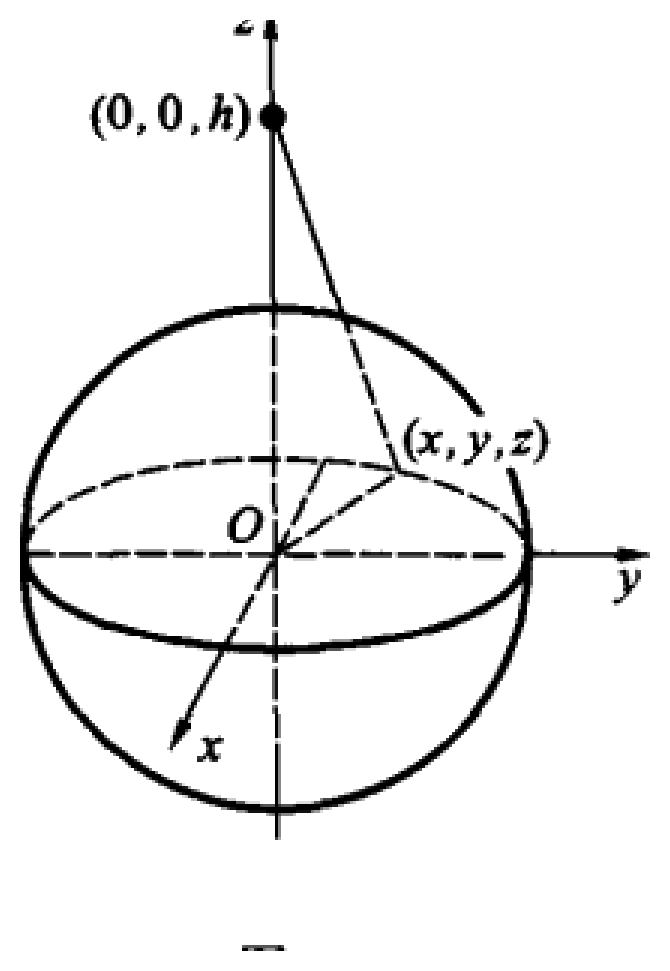
\includegraphics[width=0.45\textwidth]{work/figures/fig21-4}\caption{\relax}\label{fig:21-4}
\end{figure}

这个结果表明：均匀球壳内的任一点所受球壳的引力处于平衡状态，而均匀球壳外的点所受球壳的引力等于把球壳的全部质量集中到球心时对该点的引力．

\begin{xiti}
\item 对照重积分的基本性质写出第一型曲线积分和第一型曲面积分的类似性质．
\item 计算下列第一型曲线积分：
\begin{ziti}
\item $\displaystyle\int_{L}(x^{2}+y^{2})\,\mathrm{d}s$，其中 $L$ 是以 $(0,0)$，$(2,0)$，$(0,1)$ 为顶点的三角形；
\item $\displaystyle\int_{L}\sqrt{x^{2}+y^{2}}\,\mathrm{d}s$，其中 $L$ 是圆周 $x^{2}+y^{2}=ax$；
\item $\displaystyle\int_{L}xyz\,\mathrm{d}s$，其中 $L$ 为螺线 $x=a\cos t$，$y=a\sin t$，$z=bt$ $(0<a<b)$，$0\leqslant t\leqslant2\pi$；
\item $\displaystyle\int_{L}(x^{2}+y^{2}+z^{2})\,\mathrm{d}s$，其中 $L$ 与（3）相同；
\item $\displaystyle\int_{L}\left(x^{\frac{4}{3}}+y^{\frac{4}{3}}\right)\mathrm{d}s$，其中 $L$ 为内摆线 $x^{\frac{2}{3}}+y^{\frac{2}{3}}=a^{\frac{2}{3}}$；
\item $\displaystyle\int_{L}y^{2}\,\mathrm{d}s$，其中 $L$ 为摆线的一拱 $x=a(t-\sin t)$，$y=a(1-\cos t)$，$0\leqslant t\leqslant2\pi$；
\item $\displaystyle\int_{L}xy\,\mathrm{d}s$，其中 $L$ 为球面 $x^{2}+y^{2}+z^{2}=a^{2}$ 与平面 $x+y+z=0$ 的交线；
\item $\displaystyle\int_{L}(xy+yz+zx)\,\mathrm{d}s$，其中 $L$ 同（7）；
\item $\displaystyle\int_{L}xyz\,\mathrm{d}s$，其中 $L$ 是曲线 $x=t$，$y=\dfrac{2}{3}\sqrt{2t^{3}}$，$z=\dfrac{1}{2}t^{2}$ $(0\leqslant t\leqslant1)$；
\item $\displaystyle\int_{L}\sqrt{2y^{2}+z^{2}}\,\mathrm{d}s$，其中 $L$ 是 $x^{2}+y^{2}+z^{2}=a^{2}$ 与 $x=y$ 相交的圆周．
\end{ziti}
\item 计算下列第一型曲面积分：
\begin{ziti}
\item $\displaystyle\iint_{S}(x^{2}+y^{2})\,\mathrm{d}S$，其中 $S$ 是立体 $\sqrt{x^{2}+y^{2}}\leqslant z\leqslant1$ 的边界曲面；
\item $\displaystyle\iint_{S}\frac{\mathrm{d}S}{x^{2}+y^{2}}$，其中 $S$ 为柱面 $x^{2}+y^{2}=R^{2}$ 被平面 $z=0$ 和 $z=H$ 所截取的部分；
\item $\displaystyle\iint_{S}\left|x^{3}y^{2}z\right|\,\mathrm{d}S$，其中 $S$ 是曲面 $z=x^{2}+y^{2}$ 被平面 $z=1$ 割下的部分；
\item $\displaystyle\iint_{S}z^{2}\,\mathrm{d}S$，其中 $S$ 为螺旋面的一部分：
\[
x=u\cos v,\quad y=u\sin v,\quad z=v\quad\left(0\leqslant u\leqslant a,\,0\leqslant v\leqslant2\pi\right)
\]；
\item $\displaystyle\iint_{S}(x^{2}+y^{2})\,\mathrm{d}S$，$S$ 是球面 $x^{2}+y^{2}+z^{2}=R^{2}$．
\end{ziti}
\item 设曲线 $L$ 的方程为
\[
x=\mathrm{e}^{t}\cos t,\quad y=\mathrm{e}^{t}\sin t,\quad z=\mathrm{e}^{t}\quad\left(0\leqslant t\leqslant t_{0}\right),
\]
它在每一点的密度与该点的矢径平方成反比，且在点 $(1,0,1)$ 处为 $1$，求它的质量．
\item 设有一质量分布不均匀的半圆弧 $x=r\cos\theta$，$y=r\sin\theta$ $(0\leqslant\theta\leqslant\pi)$，其线密度 $\rho=a\theta$（$a$ 为常数），求它对原点 $(0,0)$ 处质量为 $m$ 的质点的引力．
\item 求螺线的一支 $L$：$x=a\cos t$，$y=a\sin t$，$z=\dfrac{h}{2\pi}t$ $(0\leqslant t\leqslant2\pi)$ 对 $x$ 轴的转动惯量 $I=\displaystyle\int_{L}(y^{2}+z^{2})\,\mathrm{d}s$．设此螺线的线密度是均匀的．
\item 求抛物面壳 $z=\dfrac{1}{2}(x^{2}+y^{2})$，$0\leqslant z\leqslant1$ 的质量．设此壳的密度 $\rho=z$．
\item 计算球面三角形 $x^{2}+y^{2}+z^{2}=a^{2}$，$x>0$，$y>0$，$z>0$ 的围线的重心坐标．设线密度 $\rho=1$．
\item 求均匀球壳 $x^{2}+y^{2}+z^{2}=a^{2}$ $(z\geqslant0)$ 对 $z$ 轴的转动惯量．
\item 求均匀球面 $z=\sqrt{a^{2}-x^{2}-y^{2}}$ $(x\geqslant0,\,y\geqslant0,\,x+y\leqslant a)$ 的重心坐标．
\item 若曲线以极坐标给出：$\rho=\rho(\theta)$ $(\theta_{1}\leqslant\theta\leqslant\theta_{2})$，试给出计算 $\displaystyle\int_{L}f(x,y)\,\mathrm{d}s$ 的公式，并用此公式计算下列曲线积分：
\begin{ziti}
\item $\displaystyle\int_{L}e^{\sqrt{x^{2}+y^{2}}}\,\mathrm{d}s$，其中 $L$ 是曲线 $\rho=a$ $\left(0\leqslant\theta\leqslant\dfrac{\pi}{4}\right)$；
\item $\displaystyle\int_{L}x\,\mathrm{d}s$，其中 $L$ 是对数螺线 $\rho=a\mathrm{e}^{k\theta}$ $(k>0)$ 在圆 $r=a$ 内的部分．
\end{ziti}
\item 求密度 $\rho=\rho_{0}$ 的截圆锥面 $x=r\cos\varphi$，$y=r\sin\varphi$，$z=r$ $(0\leqslant\varphi\leqslant2\pi)$，$0<b\leqslant r\leqslant a$ 对位于曲面顶点 $(0,0,0)$ 的单位质点的引力．当 $b\to0$ 时，结果如何？
\item 计算 $F(t)=\iint_{S}f(x,y,z)\,\mathrm{d}S$，其中 $S$ 是一平面 $x+y+z=t$，而
\[
f(x,y,z)=\begin{cases}
1-x^{2}-y^{2}-z^{2},&\text{当}\ x^{2}+y^{2}+z^{2}\leqslant1,\\
0,&\text{当}\ x^{2}+y^{2}+z^{2}>1.
\end{cases}
\]
\end{xiti}

\section{第二型曲线积分与曲面积分}

第一型曲线积分和曲面积分，其曲线和曲面都是无方向的，本质上与二重积分和三重积分是同类型的积分．这一节要介绍的第二型曲线积分和曲面积分，其曲线和曲面是有方向的．其实这种类型的积分我们并不陌生，定积分 $\displaystyle\int_{a}^{b}f(x)\,\mathrm{d}x$ 的区间就是有方向的：从 $a$ 到 $b$．如果反方向，便会差一个负号
\[
\int_{b}^{a}f(x)\,\mathrm{d}x=-\int_{a}^{b}f(x)\,\mathrm{d}x.
\]
曲线有方向，比较容易理解．什么叫曲面的方向？下面我们从物理背景开始，引进第二型的曲线与曲面积分．

\subsection{变力作功与第二型曲线积分}

设一质点受变力 $\bm{F}(x,y,z)$ 的作用沿空间光滑曲线段 $L$ 从点 $A$ 运动到点 $B$，变力 $\bm{F}(x,y,z)$ 不仅大小随点的变化而变化，而且方向也随点的变化而变化．这时力 $\bm{F}(x,y,z)$ 所作的功应如何计算呢？

从 $A$ 向 $B$ 给曲线弧 $L$ 一个分法：
\[
A=M_{0},M_{1},M_{2},\cdots,M_{n}=B,
\]
其中 $M_{i}=(x_{i},y_{i},z_{i})$．记 $\widehat{M_{i-1}M_{i}}$ 的弧长为 $\Delta s_{i}$，任取 $(\xi_{i},\eta_{i},\zeta_{i})\in\widehat{M_{i-1}M_{i}}$．当 $\lambda=\max\limits_{1\leqslant i\leqslant n}\{\Delta s_{i}\}$ 很小时，每个小弧段 $\widehat{M_{i-1}M_{i}}$ 上的力近似于常力 $\bm{F}(\xi_{i},\eta_{i},\zeta_{i})$，而力 $\bm{F}(x,y,z)$ 使质点沿 $\widehat{M_{i-1}M_{i}}$ 从 $M_{i-1}$ 运动到 $M_{i}$ 所作的功 $W_{i}$ 有下面的近似表达式
\[
W_{i}\approx\bm{F}(\xi_{i},\eta_{i},\zeta_{i})\cdot\overrightarrow{M_{i-1}M_{i}}.
\]
因此 $\bm{F}(x,y,z)$ 使质点从 $A$ 运动到 $B$ 所作的功
\[
W\approx\sum_{i=1}^{n}\bm{F}(\xi_{i},\eta_{i},\zeta_{i})\cdot\overrightarrow{M_{i-1}M_{i}}.
\]
$\lambda$ 越小近似程度越好．故当 $\lambda\to0$ 时，上式右端和的极限就是 $\bm{F}(x,y,z)$ 使质点从 $A$ 运动到 $B$ 所作的功．

\begin{figure}[htbp]
\centering
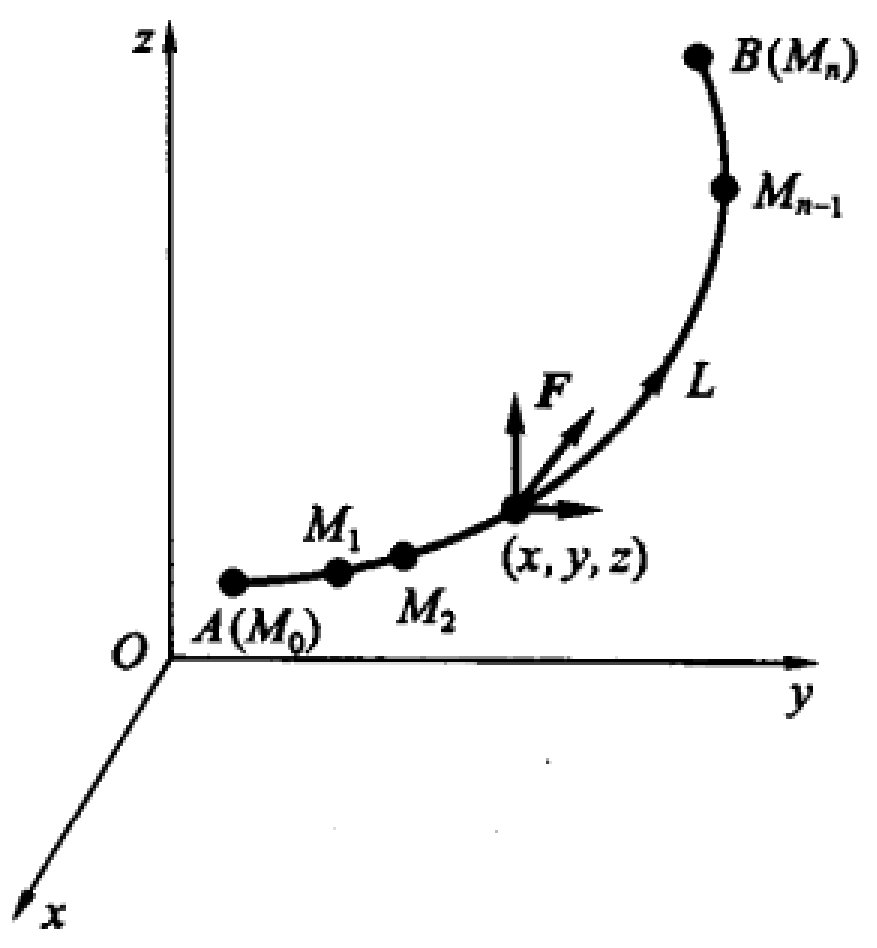
\includegraphics[width=0.4\textwidth]{work/figures/fig21-5}\caption{\relax}\label{fig:21-5}
\end{figure}

因为
\[
\begin{aligned}
\overrightarrow{M_{i-1}M_{i}}&=(x_{i}-x_{i-1},y_{i}-y_{i-1},z_{i}-z_{i-1})\\
&=(\Delta x_{i},\Delta y_{i},\Delta z_{i}),
\end{aligned}
\]
注意这时 $\Delta x_{i},\Delta y_{i},\Delta z_{i}$ 是可正可负的，大小与符号由向量 $\overrightarrow{M_{i-1}M_{i}}$ 决定．又若
\[
\bm{F}(x,y,z)=\left(P(x,y,z),Q(x,y,z),R(x,y,z)\right)
\]
则有
\[
\begin{aligned}
W&=\lim_{\lambda\to0}\sum_{i=1}^{n}\bm{F}(\xi_{i},\eta_{i},\zeta_{i})\cdot\overrightarrow{M_{i-1}M_{i}}\\
&=\lim_{\lambda\to0}\left\{\sum_{i=1}^{n}P(\xi_{i},\eta_{i},\zeta_{i})\Delta x_{i}+Q(\xi_{i},\eta_{i},\zeta_{i})\Delta y_{i}+R(\xi_{i},\eta_{i},\zeta_{i})\Delta z_{i}\right\}.
\end{aligned}
\]
抽去其中的物理背景，这样一种和的极限就引导到第二型曲线积分．

\begin{definition}\label{def:21-3}
设函数 $f(x,y,z)$ 定义在空间光滑曲线弧 $L$ 上，$L$ 的两端点为 $A$，$B$．从 $A$ 向 $B$ 给 $\widehat{AB}$ 一个分法：$A=M_{0},M_{1},\cdots,M_{n}=B$，其中 $M_{i}=(x_{i},y_{i},z_{i})$，记 $\widehat{M_{i-1}M_{i}}$ 的弧长为 $\Delta s_{i}$，$\Delta x_{i}=x_{i}-x_{i-1}$，任取 $(\xi_{i},\eta_{i},\zeta_{i})\in\widehat{M_{i-1}M_{i}}$，作和式
\[
\sigma=\sum_{i=1}^{n}f(\xi_{i},\eta_{i},\zeta_{i})\Delta x_{i}.
\]
若当 $\lambda=\max\limits_{1\leqslant i\leqslant n}\{\Delta s_{i}\}\to0$ 时，$\sigma$ 的极限存在，则称该极限为函数 $f$ 沿有向曲线 $L$ 对 $x$ 的\emph{第二型曲线积分}，记为
\[
\int_{L}f(x,y,z)\,\mathrm{d}x,
\]
或
\[
\int_{\widehat{AB}}f(x,y,z)\,\mathrm{d}x.
\]
如果在上述求和时，分别用 $\Delta y_{i}=y_{i}-y_{i-1}$ 或 $\Delta z_{i}=z_{i}-z_{i-1}$ 代替 $\Delta x_{i}$，便得到 $f$ 沿 $L$ 对 $y$ 或对 $z$ 的第二型曲线积分：
\[
\int_{L}f(x,y,z)\,\mathrm{d}y
\]
或
\[
\int_{L}f(x,y,z)\,\mathrm{d}z.
\]
\end{definition}

如果有向量函数 $\bm{F}(x,y,z)=\left(P(x,y,z),Q(x,y,z),R(x,y,z)\right)$，则根据定义~\ref{def:21-3} 有
\[
\begin{aligned}
&\int_{L}P(x,y,z)\,\mathrm{d}x+\int_{L}Q(x,y,z)\,\mathrm{d}y+\int_{L}R(x,y,z)\,\mathrm{d}z\\
={}&\lim_{\lambda\to0}\sum_{i=1}^{n}\left[P(\xi_{i},\eta_{i},\zeta_{i})\Delta x_{i}+Q(\xi_{i},\eta_{i},\zeta_{i})\Delta y_{i}+R(\xi_{i},\eta_{i},\zeta_{i})\Delta z_{i}\right],
\end{aligned}
\]
其中 $\Delta x_{i}$，$\Delta y_{i}$，$\Delta z_{i}$ 分别是向量 $\overrightarrow{M_{i-1}M_{i}}$ 在 $x$，$y$，$z$ 轴上的有向投影．若记
\[
\mathrm{d}\bm{s}=\left\{\mathrm{d}x,\mathrm{d}y,\mathrm{d}z\right\},
\]
则
\[
\begin{aligned}
&\int_{L}P(x,y,z)\,\mathrm{d}x+Q(x,y,z)\,\mathrm{d}y+R(x,y,z)\,\mathrm{d}z\\
={}&\int_{L}\bm{F}(x,y,z)\cdot\mathrm{d}\bm{s}.
\end{aligned}
\]
因此上述积分也称为向量函数 $\bm{F}(x,y,z)$ 沿有向曲线 $L$ 的积分．$\mathrm{d}\bm{s}$ 的方向就是曲线 $L$ 的切线方向，其指向与 $L$ 的方向一致．

第二型曲线积分中曲线是有方向的，这是与第一型曲线积分的根本区别所在．如果对 $L$ 的积分改为由 $B$ 到 $A$，则在上述定义中，变成了用 $\overrightarrow{M_{i}M_{i-1}}$ 的投影来代替原来的 $\overrightarrow{M_{i-1}M_{i}}$ 的投影，显然和式差了一个负号．因此对同一曲线有
\[
\int_{\widehat{AB}}P\,\mathrm{d}x+Q\,\mathrm{d}y+R\,\mathrm{d}z=-\int_{\widehat{BA}}P\,\mathrm{d}x+Q\,\mathrm{d}y+R\,\mathrm{d}z.
\]
它们恰好相差一个负号．而对第一型曲线积分来说，从 $A$ 到 $B$ 的积分与从 $B$ 到 $A$ 的积分是相等的，即
\[
\int_{\widehat{AB}}f(x,y,z)\,\mathrm{d}s=\int_{\widehat{BA}}f(x,y,z)\,\mathrm{d}s.
\]
对于闭曲线 $L$，我们常记为
\[
\oint_{L}P\,\mathrm{d}x+Q\,\mathrm{d}y+R\,\mathrm{d}z.
\]
这时积分与起点的选择无关，只与曲线 $L$ 的方向有关．

下面的定理告诉我们，连续函数沿光滑线段的第二型曲线积分总存在，并且可以化为定积分来计算．

\begin{theorem}\label{thm:21-3}
设 $f(x,y,z)$ 是定义在光滑曲线段
\[
\widehat{AB}:x=x(t),\ y=y(t),\ z=z(t),\quad\alpha\leqslant t\leqslant\beta
\]
上的连续函数，$t=\alpha$ 时对应于 $A$ 点，$t=\beta$ 时对应于 $B$ 点，且 $\widehat{AB}$ 自身不相交，则 $f$ 沿 $\widehat{AB}$ 的第二型曲线积分 $\displaystyle\int_{\widehat{AB}}f(x,y,z)\,\mathrm{d}x$ 存在，且有
\[
\int_{\widehat{AB}}f(x,y,z)\,\mathrm{d}x=\int_{\alpha}^{\beta}f(x(t),y(t),z(t))x^{\prime}(t)\,\mathrm{d}t.
\]
\end{theorem}

\begin{proof}
从 $A$ 向 $B$ 任给 $\widehat{AB}$ 一个分法 $A=M_{0},M_{1},\cdots,M_{n}=B$，$M_{i}=(x_{i},y_{i},z_{i})$ $(i=0,1,\cdots,n)$，则相应地得到 $[\alpha,\beta]$ 的一个分法：
\[
\alpha=t_{0}<t_{1}<\cdots<t_{n}=\beta,
\]
使得 $M_{i}=(x(t_{i}),y(t_{i}),z(t_{i}))$ $(i=1,2,\cdots,n)$．由于 $\widehat{AB}$ 自身不相交，故上述 $M_{i}$ 与 $t_{i}$ 是一一对应的．任取 $(\xi_{i},\eta_{i},\zeta_{i})\in\widehat{M_{i-1}M_{i}}$，存在 $\tau_{i}\in[t_{i-1},t_{i}]$，使
\[
(\xi_{i},\eta_{i},\zeta_{i})=(x(\tau_{i}),y(\tau_{i}),z(\tau_{i})).
\]
因此
\[
\begin{aligned}
\sigma&=\sum_{i=1}^{n}f(\xi_{i},\eta_{i},\zeta_{i})\Delta x_{i}\\
&=\sum_{i=1}^{n}f(x(\tau_{i}),y(\tau_{i}),z(\tau_{i}))\left(x(t_{i})-x(t_{i-1})\right).
\end{aligned}
\]
由于 $\widehat{AB}$ 是光滑曲线，$x(t)$ 在 $[\alpha,\beta]$ 有连续导数，由拉格朗日中值定理，存在 $\tau_{i}^{*}\in[t_{i-1},t_{i}]$，使
\[
x(t_{i})-x(t_{i-1})=x^{\prime}(\tau_{i}^{*})(t_{i}-t_{i-1})=x^{\prime}(\tau_{i}^{*})\Delta t_{i}.
\]
因此
\[
\sigma=\sum_{i=1}^{n}f(x(\tau_{i}),y(\tau_{i}),z(\tau_{i}))x^{\prime}(\tau_{i}^{*})\Delta t_{i}.
\]
记 $\lambda=\max\limits_{1\leqslant i\leqslant n}\{\Delta s_{i}\}$，$\lambda'=\max\limits_{1\leqslant i\leqslant n}\{\Delta t_{i}\}$，因为 $\widehat{AB}$ 是光滑曲线，故当 $\lambda\to0$ 时有 $\lambda'\to0$．又由于 $f(x(t),y(t),z(t))$，$x'(t)$ 都在 $[\alpha,\beta]$ 连续，虽然 $\tau_{i}$，$\tau_{i}^{*}\in[t_{i-1},t_{i}]$ 不一定相同，但像我们以前证明过多次的一样，$\sigma$ 的极限是存在的，且
\[
\begin{aligned}
&\lim_{\lambda\to0}\sum_{i=1}^{n}f(x(\tau_{i}),y(\tau_{i}),z(\tau_{i}))x^{\prime}(\tau_{i}^{*})\Delta t_{i}\\
={}&\int_{\alpha}^{\beta}f(x(t),y(t),z(t))x^{\prime}(t)\,\mathrm{d}t.
\end{aligned}
\]
而根据定义，$\sigma$ 的极限是曲线积分 $\displaystyle\int_{\widehat{AB}}f(x,y,z)\,\mathrm{d}x$，这就完成了定理~\ref{thm:21-3} 的证明．
\end{proof}

类似地可以证明在定理~\ref{thm:21-3} 的条件下有
\[
\int_{\widehat{AB}}f(x,y,z)\,\mathrm{d}y=\int_{\alpha}^{\beta}f(x(t),y(t),z(t))y^{\prime}(t)\,\mathrm{d}t.
\]
\[
\int_{\widehat{AB}}f(x,y,z)\,\mathrm{d}z=\int_{\alpha}^{\beta}f(x(t),y(t),z(t))z^{\prime}(t)\,\mathrm{d}t.
\]
要特别强调的是公式右端定积分的下限总是对应有向曲线段的起点，上限总是对应有向曲线段的终点．

如果曲线 $L$ 是分段光滑的有向曲线，那么 $L$ 是有限条光滑曲线段连结而成且上一段的终点是下一段的起点，这时公式仍然成立．事实上只要逐段地应用上述公式再对积分值求和即可．

\begin{example}\label{ex:21-3-1}
求 $\displaystyle\int_{\widehat{AB}}(x^{2}+y^{2})\,\mathrm{d}x+4xy\,\mathrm{d}y$，其中
\begin{ziti}
\item $\widehat{AB}$ 是上半圆周 $x^{2}+y^{2}=ax$ $(y\geqslant0)$，
\item $\widehat{AB}$ 是直线段 $y=0$ $(0\leqslant x\leqslant a)$，
\end{ziti}
方向如图~\ref{fig:21-6} 所示．
\end{example}

\begin{figure}[htbp]
\centering
\begin{tikzpicture}[scale=1]
\draw[->,thick] (-0.4,0) -- (3.4,0) node[below] {$x$};
\draw[->,thick] (0,-0.4) -- (0,1.9) node[left] {$y$};
\draw[thick] (0,0) arc (180:0:1.5);
\draw[thick,->] ({1.5+1.5*cos(100)},{1.5*sin(100)}) arc (100:80:1.5);
\fill (0,0) circle (1.2pt) node[below left] {$A$};
\fill (3,0) circle (1.2pt) node[above right] {$B$};
\node[below] at (3,-0.05) {$a$};
\draw[thick,->] (1.3,0) -- (1.7,0);
\end{tikzpicture}\caption{\relax}\label{fig:21-6}
\end{figure}

\begin{proof}[解]
（1）取 $\widehat{AB}$ 的参数方程为
\[
\begin{cases}
x=x,\\
y=\sqrt{ax-x^{2}},
\end{cases}
\quad 0\leqslant x\leqslant a.
\]
\[
\begin{aligned}
&\int_{\widehat{AB}}\left(x^{2}+y^{2}\right)\mathrm{d}x+4xy\,\mathrm{d}y\\
={}&\int_{0}^{a}\left[x^{2}+\left(ax-x^{2}\right)+4x\sqrt{ax-x^{2}}\,\frac{a-2x}{2\sqrt{ax-x^{2}}}\right]\mathrm{d}x\\
={}&\int_{0}^{a}(3ax-4x^{2})\,\mathrm{d}x=\frac{a^{3}}{6}.
\end{aligned}
\]
我们也可以取 $\widehat{AB}$ 的参数方程为
\[
\begin{cases}
x=\dfrac{a}{2}+\dfrac{a}{2}\cos\theta,\\
y=\dfrac{a}{2}\sin\theta,
\end{cases}
\quad 0\leqslant\theta\leqslant\pi.
\]
注意 $\theta=\pi$ 时对应于 $A$ 点，$\theta=0$ 时对应于 $B$ 点，因此
\[
\begin{aligned}
&\int_{\widehat{AB}}\left(x^{2}+y^{2}\right)\mathrm{d}x+4xy\,\mathrm{d}y\\
={}&\int_{\pi}^{0}\left\{\left[\left(\frac{a}{2}+\frac{a}{2}\cos\theta\right)^{2}+\left(\frac{a}{2}\sin\theta\right)^{2}\right]\left(-\frac{a}{2}\sin\theta\right)+\right.\\
&\left.\phantom{\int_{\pi}^{0}}4\left(\frac{a}{2}+\frac{a}{2}\cos\theta\right)\frac{a}{2}\sin\theta\,\frac{a}{2}\cos\theta\right\}\mathrm{d}\theta\\
={}&\int_{\pi}^{0}\left(\frac{a}{2}\right)^{3}\left[-(2+2\cos\theta)\sin\theta+4(1+\cos\theta)\sin\theta\cos\theta\right]\mathrm{d}\theta\\
={}&\left(\frac{a}{2}\right)^{3}\int_{\pi}^{0}\left(-2\sin\theta+4\cos^{2}\theta\sin\theta\right)\mathrm{d}\theta\\
={}&\left(\frac{a}{2}\right)^{3}\left[2\cos\theta-\frac{4}{3}\cos^{3}\theta\right]\Bigg|_{\pi}^{0}=\frac{a^{3}}{6},
\end{aligned}
\]
其中第三个等式用到了正交性
\[
\int_{0}^{\pi}\sin\theta\cos\theta\,\mathrm{d}\theta=0.
\]
（2）因为 $y=0$，$\mathrm{d}y=0$，故
\[
\int_{\widehat{AB}}\left(x^{2}+y^{2}\right)\mathrm{d}x+4xy\,\mathrm{d}y=\int_{0}^{a}x^{2}\,\mathrm{d}x=\frac{x^{3}}{3}\bigg|_{0}^{a}=\frac{a^{3}}{3}.
\]
\end{proof}

从此例可见尽管两曲线的起点和终点相同．但由于路径不同，积分值可能不同．进一步（1）、（2）中的两曲线段构成封闭曲线 $L$，则沿 $L$ 的逆时针方向有
\[
\int_{L}\left(x^{2}+y^{2}\right)\mathrm{d}x+4xy\,\mathrm{d}y=-\frac{a^{3}}{6}+\frac{a^{3}}{3}=\frac{a^{3}}{6}.
\]

\begin{example}\label{ex:21-3-2}
求在力 $\bm{F}=(y,-x,x+y+z)$ 的作用下，质点由 $A$ 到 $B$ 所作的功（图~\ref{fig:21-7}）：
\begin{ziti}
\item $\widehat{AB}$ 是螺旋线
\[
L_{1}:x=a\cos t,\quad y=a\sin t,\quad z=bt,\quad 0\leqslant t\leqslant2\pi;
\]
\item $\widehat{AB}$ 是直线段
\[
L_{2}:\ x=a,\ y=0,\ z=t,\ 0\leqslant t\leqslant2\pi b.
\]
\end{ziti}
\end{example}

\begin{figure}[htbp]
\centering
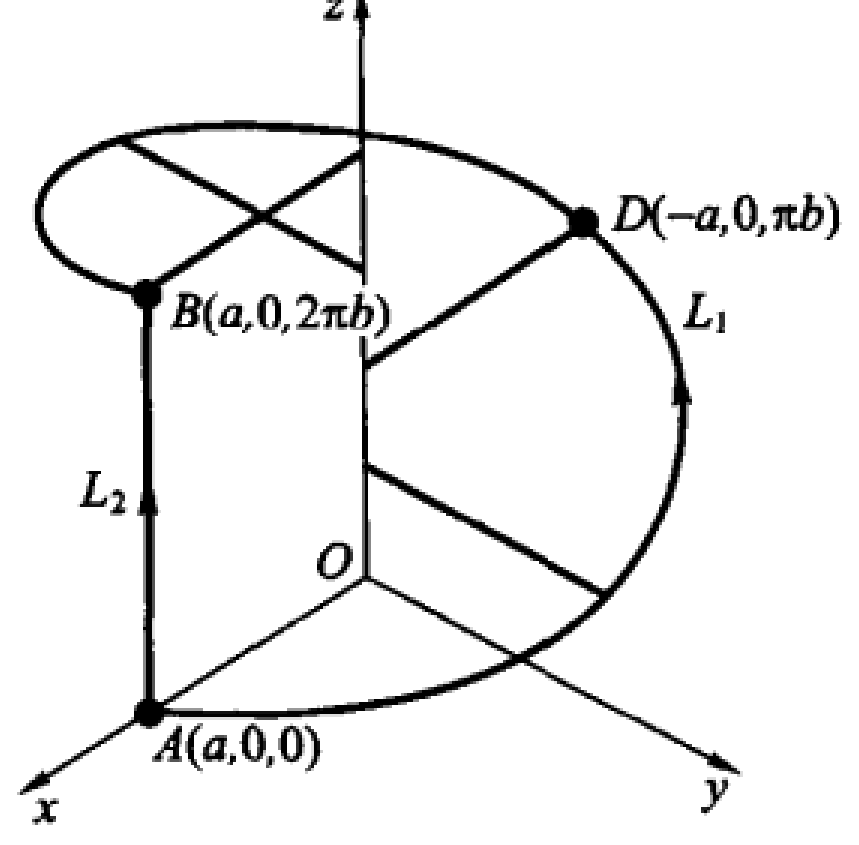
\includegraphics[width=0.45\textwidth]{work/figures/fig21-7}\caption{\relax}\label{fig:21-7}
\end{figure}

\begin{proof}[解]
（1）
\[
\begin{aligned}
W&=\int_{L_{1}}\bm{F}\cdot\mathrm{d}\bm{s}\\
&=\int_{L_{1}}y\,\mathrm{d}x-x\,\mathrm{d}y+(x+y+z)\,\mathrm{d}z\\
&=\int_{0}^{2\pi}\left[-(a\sin t)^{2}-(a\cos t)^{2}+\right.\\
&\quad\left.\left(a\cos t+a\sin t+bt\right)b\right]\mathrm{d}t\\
&=\int_{0}^{2\pi}\left(-a^{2}+b^{2}t\right)\mathrm{d}t=2\pi(\pi b^{2}-a^{2}).
\end{aligned}
\]
（2）
\[
\begin{aligned}
W&=\int_{L_{2}}\bm{F}\cdot\mathrm{d}\bm{s}\\
&=\int_{L_{2}}y\,\mathrm{d}x-x\,\mathrm{d}y+(x+y+z)\,\mathrm{d}z\\
&=\int_{0}^{2\pi b}(a+t)\,\mathrm{d}t=2\pi b(a+\pi b).
\end{aligned}
\]
\end{proof}

我们曾经强调，从概念上说两型曲线积分是很不同的，但它们的计算都是化为定积分来完成，因此两者之间是有联系的．下面我们以定积分为桥梁，寻求两者之间的联系．

设光滑曲线段 $\widehat{AB}$ 的弧长为 $l$，$M$ 是 $\widehat{AB}$ 上的点．取弧长 $s=\widehat{AM}$ 为参数，得 $\widehat{AB}$ 的本性方程
\[
\begin{cases}
x=x(s),\\
y=y(s),\\
z=z(s),
\end{cases}
\quad 0\leqslant s\leqslant l.
\]
这时 $s$ 增加的方向就是 $\widehat{AB}$ 的方向．设 $P$，$Q$，$R$ 在 $\widehat{AB}$ 上连续，由第二型曲线积分的计算公式有
\[
\int_{\widehat{AB}}P(x,y,z)\,\mathrm{d}x=\int_{0}^{l}P(x(s),y(s),z(s))x^{\prime}(s)\,\mathrm{d}s,
\]
\[
\int_{\widehat{AB}}Q(x,y,z)\,\mathrm{d}y=\int_{0}^{l}Q(x(s),y(s),z(s))y^{\prime}(s)\,\mathrm{d}s,
\]
\[
\int_{\widehat{AB}}R(x,y,z)\,\mathrm{d}z=\int_{0}^{l}R(x(s),y(s),z(s))z^{\prime}(s)\,\mathrm{d}s.
\]
已知在 $M$ 点曲线的切向量为 $\bm{\tau}=(x^{\prime}(s),y^{\prime}(s),z^{\prime}(s))$，其方向与 $s$ 增加的方向一致，也就是 $\widehat{AB}$ 的方向．由于参数是弧长，而弧长
\[
s=\int_{0}^{s}\sqrt{x^{\prime2}(t)+y^{\prime2}(t)+z^{\prime2}(t)}\,\mathrm{d}t,
\]
因此
\[
\mathrm{d}s=\sqrt{x^{\prime2}(s)+y^{\prime2}(s)+z^{\prime2}(s)}\,\mathrm{d}s,
\]
即 $x^{\prime2}(s)+y^{\prime2}(s)+z^{\prime2}(s)=1$，这表明 $\bm{\tau}$ 是单位向量．用 $(\bm{\tau},x)$，$(\bm{\tau},y)$，$(\bm{\tau},z)$ 分别表示 $\bm{\tau}$ 与 $x$，$y$，$z$ 轴正向的夹角，就有
\[
\begin{aligned}
\bm{\tau}&=\left(x^{\prime}(s),y^{\prime}(s),z^{\prime}(s)\right)\\
&=\left(\cos(\bm{\tau},x),\cos(\bm{\tau},y),\cos(\bm{\tau},z)\right),
\end{aligned}
\]
故
\begin{align}
&\int_{\widehat{AB}}P\,\mathrm{d}x+Q\,\mathrm{d}y+R\,\mathrm{d}z\notag\\
={}&\int_{0}^{l}\left[Px^{\prime}(s)+Qy^{\prime}(s)+Rz^{\prime}(s)\right]\mathrm{d}s\tag{1}\label{eq:21-2-1}\\
={}&\int_{\widehat{AB}}\left[P\cos(\bm{\tau},x)+Q\cos(\bm{\tau},y)+R\cos(\bm{\tau},z)\right]\mathrm{d}s.\notag
\end{align}
注意等式的最左端是第二型曲线积分，最右端是第一型曲线积分，中间则是定积分．这样我们就给出了两型曲线积分之间的联系．读者可能会发生疑问，最左端的第二型曲线积分是与曲线方向有关的，而右端的第一型曲线积分是与曲线方向无关的，它们怎么能相等呢？事实上，如果积分由 $\widehat{AB}$ 改为 $\widehat{BA}$，最左端积分改变符号，但请注意这时 $\bm{\tau}$ 的方向也变成了反向，也就是说 $\left(\cos(\bm{\tau},x),\cos(\bm{\tau},y),\cos(\bm{\tau},z)\right)$ 也改变了符号．因此，虽然第一型积分不变号，但被积函数改变了符号，等式仍然成立．

如果用矢量形式表示，则上式还可以有更简捷的形式：
\begin{equation}\label{eq:21-2-2}
\int_{\widehat{AB}}\bm{F}\cdot\mathrm{d}\bm{s}=\int_{\widehat{AB}}\bm{F}\cdot\bm{\tau}\,\mathrm{d}s,
\tag{2}
\end{equation}
其中 $\bm{\tau}$ 是与 $\widehat{AB}$ 方向一致的单位切向量．记
\[
\mathrm{d}\bm{s}=\bm{\tau}\,\mathrm{d}s,
\]
用分量表示就是
\[
(\mathrm{d}x,\mathrm{d}y,\mathrm{d}z)=\left(\cos(\bm{\tau},x),\cos(\bm{\tau},y),\cos(\bm{\tau},z)\right)\mathrm{d}s,
\]
或
\[
\cos(\bm{\tau},x)=\frac{\mathrm{d}x}{\mathrm{d}s},\quad\cos(\bm{\tau},y)=\frac{\mathrm{d}y}{\mathrm{d}s},\quad\cos(\bm{\tau},z)=\frac{\mathrm{d}z}{\mathrm{d}s}.
\]
它们就是公式\eqref{eq:21-2-1}、\eqref{eq:21-2-2}的微分表示，其几何意义是很清楚的．$\mathrm{d}\bm{s}$ 的方向与 $\bm{\tau}$ 的方向一致，而 $\mathrm{d}x$，$\mathrm{d}y$，$\mathrm{d}z$ 分别是 $\mathrm{d}\bm{s}$ 按 $\bm{\tau}$ 的方向在 $x$，$y$，$z$ 轴上的有向投影（图~\ref{fig:21-8}）．

\begin{figure}[htbp]
\centering
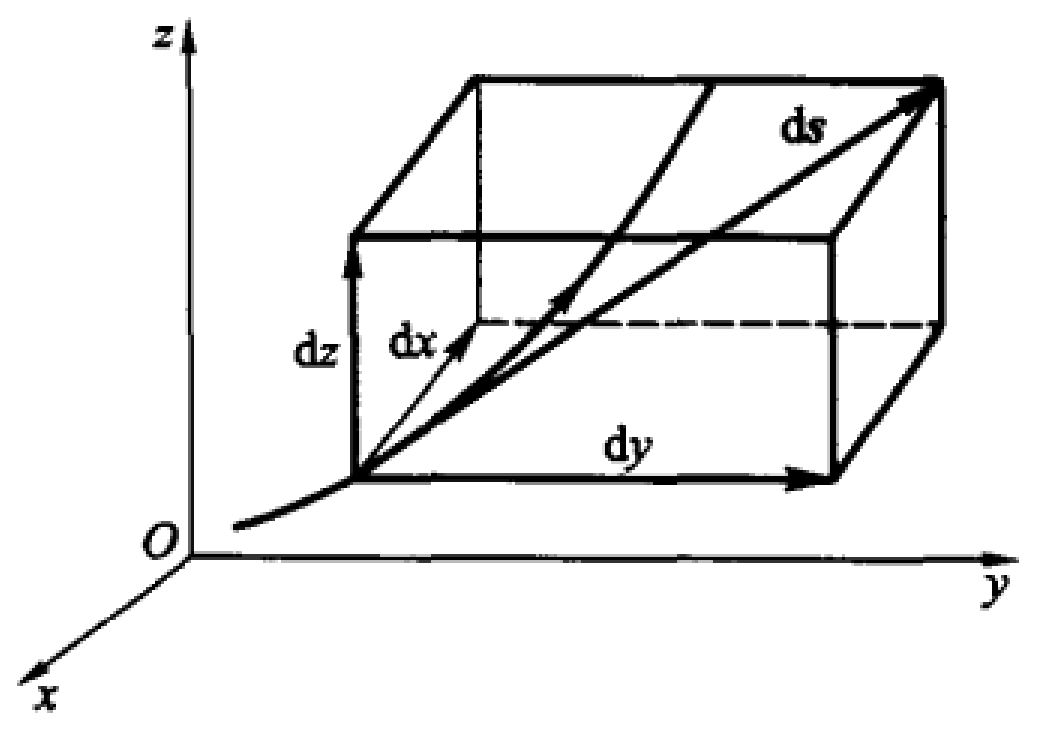
\includegraphics[width=0.5\textwidth]{work/figures/fig21-8}\caption{\relax}\label{fig:21-8}
\end{figure}

特别地，当 $\widehat{AB}$ 是平面曲线时，$\cos(\bm{\tau},z)=0$，则有
\[
\int_{\widehat{AB}}P\,\mathrm{d}x+Q\,\mathrm{d}y=\int_{\widehat{AB}}\left[P\cos(\bm{\tau},x)+Q\cos(\bm{\tau},y)\right]\mathrm{d}s.
\]

\begin{example}\label{ex:21-3-3}
求 $\displaystyle\oint_{L}\frac{x\,\mathrm{d}x+y\,\mathrm{d}y}{x^{2}+y^{2}}$，其中 $L$ 是 $x^{2}+y^{2}=a^{2}$ 沿逆时针方向．
\end{example}

\begin{proof}[解]
令
\[
\bm{F}=(P,Q)=\left(\frac{x}{x^{2}+y^{2}},\frac{y}{x^{2}+y^{2}}\right)=\frac{\bm{r}}{r^{2}},
\]
其中 $\bm{r}=\left\{x,y\right\}$ 是 $L$ 上点的向径，由于圆上每点的切线垂直于向径 $\bm{r}$，即 $\bm{r}\cdot\bm{\tau}=0$，因此由两种曲线积分的联系得
\[
\int_{L}\frac{x\,\mathrm{d}x+y\,\mathrm{d}y}{x^{2}+y^{2}}=\int_{L}\frac{1}{a^{2}}\bm{r}\cdot\bm{\tau}\,\mathrm{d}s=0.
\]
\end{proof}

\begin{figure}[htbp]
\centering
\begin{tikzpicture}[scale=1]
\draw[->,thick] (-2.2,0) -- (2.4,0) node[below] {$x$};
\draw[->,thick] (0,-1.9) -- (0,2.1) node[left] {$y$};
\draw[thick] (0,0) circle (1.6);
\draw[->,thick] (0,0) -- (50:1.6) node[midway,above left] {$\bm{r}$};
\fill (50:1.6) circle (1.2pt);
\draw[->,thick] (50:1.6) -- ++(140:0.9) node[above] {$\bm{\tau}$};
\node[below left] at (0,0) {$O$};
\node[below] at (1.6,0) {$a$};
\end{tikzpicture}\caption{\relax}\label{fig:21-9}
\end{figure}

\subsection{流量与第二型曲面积分}

先从一个物理问题谈起．

设空间有一块流体．如果对于空间区域 $V$ 的每一点 $(x,y,z)$ 与每一时刻 $t$，都对应一个流体的速度向量 $\bm{v}(x,y,z,t)$，那么就称流体在 $V$ 确定了一个速度的向量场 $\bm{v}(x,y,z,t)$．用数学的语言说，一个速度向量场就是一个定义在空间某区域 $V$ 上的向量值函数，另外，它可能还依赖于参数——时间 $t$．在研究江河海洋的水流运动中，在研究大气的运动中（天气预报、台风预报等），在研究爆炸过程激波的产生与运动中，速度场是常见的一个量．如果速度场不依赖于 $t$，即 $\bm{v}$ 仅是 $x$，$y$，$z$ 的函数，则称速度场是\emph{定常}的；如果速度场不仅依赖于 $x$，$y$，$z$ 还依赖于时间 $t$，则称速度场是\emph{不定常}的．研究工作总是从简单到复杂，因此，人们首先研究定常的速度场．一个最简单的物理问题是，设在一定常的速度场的定义域内，有一光滑的曲面 $S$，我们问，单位时间流过 $S$ 的流体是多少？如何计算？也就是说，如何计算流体通过 $S$ 的流量．

为解决这个问题，首先遇到的问题是，什么叫做流过（或通过）？直观的理解是从曲面的一侧到曲面的另一侧．然则什么叫曲面的侧？曲面永远都有两侧吗？

先假设 $S$ 不是闭曲面，这时它的边缘由逐段光滑的曲线 $L$ 构成．由于曲面 $S$ 是光滑的，因此在 $S$ 的每一点 $M$ 都有切平面，且切平面的位置随切点的位置而连续地变动．自然，在 $S$ 的每一点 $M$ 也有两个相反方向的单位法向量，它们是否分别代表了曲面在 $M$ 点的两侧？问题在于什么是曲面的侧．由于曲面 $S$ 是光滑的，曲面上两点 $M_{1}$ 与 $M_{2}$，它们上面分别有取定方向的两个法向量 $\bm{n}_{1}$，$\bm{n}_{2}$．如果在曲面上沿光滑曲线 $\Gamma$ 由 $M_{1}$ 运动到 $M_{2}$，则法向量 $\bm{n}_{1}$ 连续地变化．当它变到 $M_{2}$ 时，若法向量与 $\bm{n}_{2}$ 同向，自然便认为 $\bm{n}_{1}$ 与 $\bm{n}_{2}$ 是在曲面的同侧（图~\ref{fig:21-10}）；若 $\bm{n}_{1}$ 连续运动至 $M_{2}$ 时的法向量与 $\bm{n}_{2}$ 反向，自然便认为 $\bm{n}_{1}$ 与 $\bm{n}_{2}$ 是在曲面的异侧．因此，在曲面上取定点 $M_{1}$，在 $M_{1}$ 取定一法向量 $\bm{n}_{1}$，则由 $M_{1}$ 沿 $S$ 的光滑曲线而不越过 $S$ 的边缘，连续地走遍 $S$，便得到了 $S$ 中与 $\bm{n}_{1}$ 同侧的全体法向量．通常，人们会认为，对与 $\bm{n}_{1}$ 反向的 $-\bm{n}_{1}$，用同样的办法，即由 $M_{1}$ 出发沿 $S$ 的光滑曲线而不越过曲面的边缘，连续地走遍 $S$，便得到了 $S$ 中与 $-\bm{n}_{1}$ 同向的全体法向量．这样，便把曲面的两侧区分开来了．

\begin{figure}[htbp]
\centering
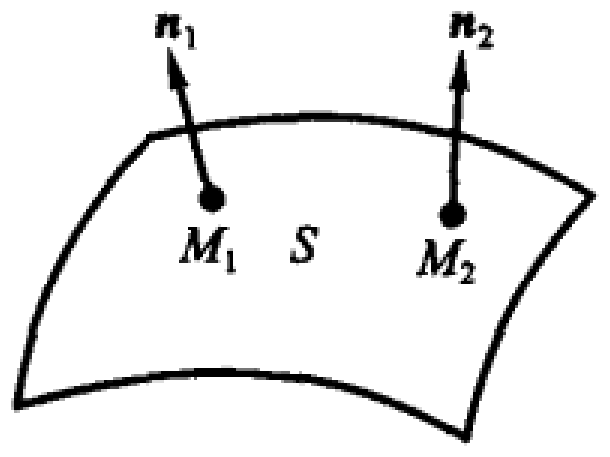
\includegraphics[width=0.4\textwidth]{work/figures/fig21-10}\caption{\relax}\label{fig:21-10}
\end{figure}

现在，问题在于，从 $M_{1}$ 出发，$\bm{n}_{1}$ 沿 $S$ 的光滑曲线而不越过曲面的边缘连续地变化，是否可能回到 $M_{1}$ 时变成了 $-\bm{n}_{1}$？也就是说，$\bm{n}_{1}$ 与 $-\bm{n}_{1}$ 可能在曲面的同一侧．换句话说，是否存在曲面，它不是双侧的而是单侧的．所谓\emph{默比乌斯}（Möbius，A.F.，1790—1868）带就是这种单侧曲面的曲型例子．将长方形纸条 $ABCD$ 先扭转一次，然后使 $B$ 与 $D$ 及 $A$ 与 $C$ 粘合起来（图~\ref{fig:21-11}），构成一条非闭的环带，便是默比乌斯带了．它的确具有上述单侧曲面的性质．假如用一种颜色涂这条环带，则可以不越过边缘而涂遍它的全部．对单侧曲面，自然不便说流体``通过''它的流量，因此，本书以后只讨论双侧曲面，除特别说明外，曲面都是指双侧的．

\begin{figure}[htbp]
\centering
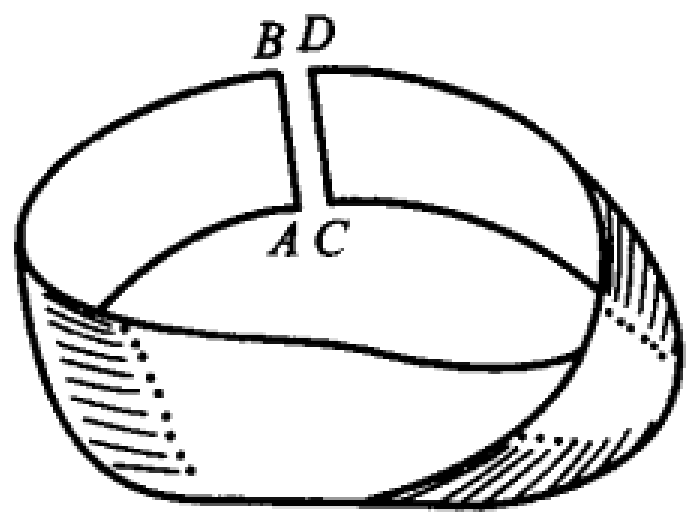
\includegraphics[width=0.4\textwidth]{work/figures/fig21-11}\caption{\relax}\label{fig:21-11}
\end{figure}

设 $S$ 是一双侧曲面，根据上面对曲面的侧的描述，如果在 $S$ 上任一点 $M_{1}$ 的法线上选定了一个确定的方向，则曲面上全部点的同侧法线也随之确定，也就是选定了曲面的一侧；如果原先选定的法线方向改变，则在其它点的法线方向也一律改变，这样就确定了曲面的另一侧．故对双侧曲面要确定它的一侧，只要在它上面任一点确定一法线方向就行了．

下面研究实际上怎样确定曲面的侧．设光滑曲面由函数
\[
z=f(x,y),\ (x,y)\in D
\]
确定，其中 $f(x,y)$ 在 $D$ 有连续的偏导数
\[
p=\frac{\partial f}{\partial x},\quad q=\frac{\partial f}{\partial y}.
\]
这样，曲面在每一点都有切平面，从而在每一点都有确定的法线．由第十六章 §3 知，曲面 $S$ 的单位法向量为
\[
\begin{aligned}
&\left(\cos\alpha,\cos\beta,\cos\gamma\right)\\
={}&\left(\frac{-p}{\pm\sqrt{1+p^{2}+q^{2}}},\frac{-q}{\pm\sqrt{1+p^{2}+q^{2}}},\frac{1}{\pm\sqrt{1+p^{2}+q^{2}}}\right).
\end{aligned}
\]
可见只要取定根式前正负号，三个分量都是 $x$，$y$ 的连续函数，也就是说法线的方向是随点的位置而连续变动的．因此，根式前正负号的选择，便表示确定了曲面的一侧．例如，若选取正号，则 $\cos\gamma>0$，它表示法向与 $z$ 轴正向交角为锐角，这就是通常所说的曲面的上侧．若选取负号，则所确定的一侧是曲面的下侧．这时法线与 $z$ 轴正向的交角是钝角．

设光滑曲面由参数方程
\[
x=x(u,v),\quad y=y(u,v),\quad z=z(u,v),\quad(u,v)\in\Delta
\]
给出．记
\[
A=\frac{\partial(y,z)}{\partial(u,v)},\quad B=\frac{\partial(z,x)}{\partial(u,v)},\quad C=\frac{\partial(x,y)}{\partial(u,v)}.
\]
由曲面光滑知 $A^{2}+B^{2}+C^{2}\neq0$，这时曲面 $S$ 上的单位法向量为
\[
\bm{n}=\left(\frac{A}{\pm\sqrt{A^{2}+B^{2}+C^{2}}},\frac{B}{\pm\sqrt{A^{2}+B^{2}+C^{2}}},\frac{C}{\pm\sqrt{A^{2}+B^{2}+C^{2}}}\right).
\]
只要取定根式前的正负号，则三个分量都是 $u$，$v$ 的连续函数，也就是说法线的方向随点的位置而连续移动．这样，如果选正号，则表示选定了曲面的一侧，如果选负号，则表示选定了曲面的另一侧．至于正号对应于曲面的哪一侧，只要选一点计算出 $\bm{n}$，再在图形上把 $\bm{n}$ 表示出来，便知道正号对应的是哪一侧．

对于封闭曲面，通常把两侧分为内侧和外侧，即法向量指向曲面所围立体的内部的一侧为内侧，而另一侧为外侧．例如球面 $x^{2}+y^{2}+z^{2}=R^{2}$ 的内侧，对上半球面 $(z>0)$ 是下侧，而对下半球面 $(z<0)$ 是上侧．容易看出，无论是内侧或外侧，单位法向量是随着点在球面上移动而连续变化的．

现在我们可以计算流体的速度场为 $\bm{v}(x,y,z)$ 时的流量问题了．设 $S$ 是双侧曲面，取定一侧为正侧，这时对应的单位法向量 $\bm{n}=(\cos\alpha,\cos\beta,\cos\gamma)$ 的每一个分量都是曲面上点 $(x,y,z)$ 的连续函数．设
\[
\bm{v}(x,y,z)=\left(P(x,y,z),Q(x,y,z),R(x,y,z)\right),
\]
其中 $P$，$Q$，$R$ 在 $S$ 上连续．我们要求流体在单位时间内从 $S$ 的负侧流向正侧的流量．

任给 $S$ 一个分法 $\Delta S_{i}$ $(i=1,2,\cdots,n)$，其面积仍记为 $\Delta S_{i}$．任取 $(\xi_{i},\eta_{i},\zeta_{i})\in\Delta S_{i}$，在这点的流速向量为 $\bm{v}(\xi_{i},\eta_{i},\zeta_{i})$，在这点的单位法向量为 $\bm{n}(\xi_{i},\eta_{i},\zeta_{i})$．当 $\Delta S_{i}$ 的直径很小时，可以把 $\Delta S_{i}$ 看成切平面上的一小块面积为 $\Delta S_{i}$ 的小区域，而在这小块区域内每点的流速是不变的，可取为 $\bm{v}(\xi_{i},\eta_{i},\zeta_{i})$．这样，单位时间流过 $\Delta S_{i}$ 的流体应该填满以 $\Delta S_{i}$ 为底，以 $\left|\bm{v}(\xi_{i},\eta_{i},\zeta_{i})\right|$ 为斜长的一个柱体（见图~\ref{fig:21-12}）．已知 $\Delta S_{i}$ 的法向量为 $\bm{n}(\xi_{i},\eta_{i},\zeta_{i})$，则不难看出，这个斜柱体的体积为
\[
\bm{v}(\xi_{i},\eta_{i},\zeta_{i})\Delta S_{i}\cdot\bm{n}(\xi_{i},\eta_{i},\zeta_{i}),
\]
也就是单位时间流过 $\Delta S_{i}$ 的流量．值得注意的是，这个量可正可负．如果是正的，这时 $\bm{v}$ 和 $\bm{n}$ 的交角是锐角，它表示流体由负侧流到正侧．如果是负的，这时 $\bm{v}$ 与 $\bm{n}$ 的交角是钝角，它表示流体由正侧流到负侧．但无论如何它的大小是单位时间流过 $\Delta S_{i}$ 的流量．因此单位时间流过整个 $S$ 的流量近似等于
\[
\sigma=\sum_{i=1}^{n}\bm{v}(\xi_{i},\eta_{i},\zeta_{i})\cdot\bm{n}(\xi_{i},\eta_{i},\zeta_{i})\Delta S_{i}.
\]
当 $\lambda=\max\limits_{1\leqslant i\leqslant n}\left\{d(\Delta S_{i})\right\}\to0$ 时（其中 $d(\Delta S_{i})$ 表示 $\Delta S_{i}$ 的直径），上述和式的极限便应该等于单位时间流过 $S$ 的流量．

\begin{figure}[htbp]
\centering
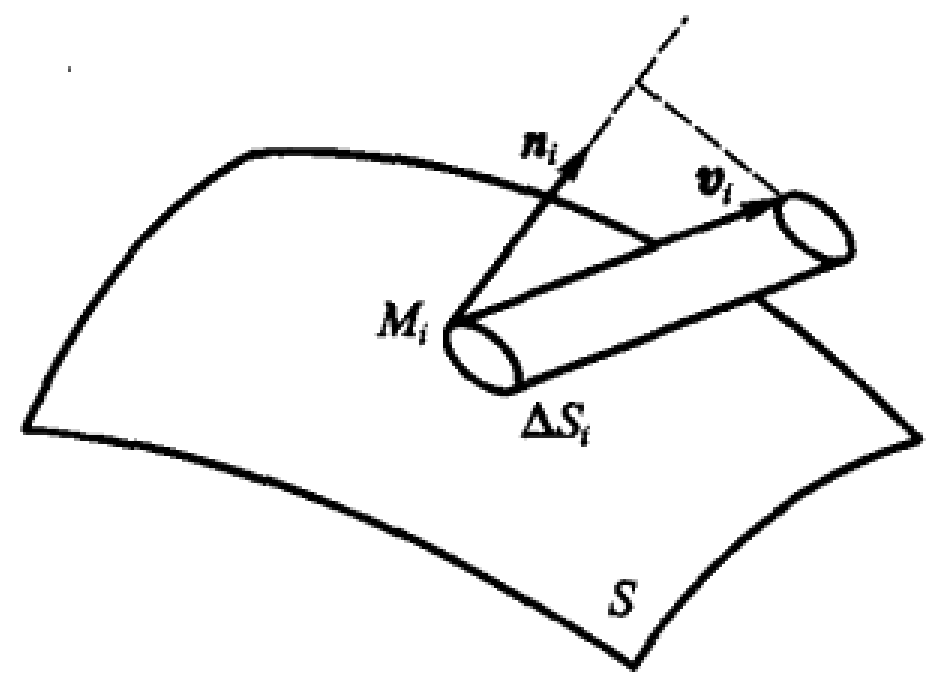
\includegraphics[width=0.5\textwidth]{work/figures/fig21-12}\caption{\relax}\label{fig:21-12}
\end{figure}

下面我们把和式 $\sigma$ 用分量表示出来．记
\[
\bm{n}(\xi_{i},\eta_{i},\zeta_{i})=\left(\cos\alpha_{i},\cos\beta_{i},\cos\gamma_{i}\right),
\]
则
\begin{align}
&\bm{v}(\xi_{i},\eta_{i},\zeta_{i})\cdot\bm{n}(\xi_{i},\eta_{i},\zeta_{i})\Delta S_{i}\notag\\
={}&P(\xi_{i},\eta_{i},\zeta_{i})\cos\alpha_{i}\Delta S_{i}+Q(\xi_{i},\eta_{i},\zeta_{i})\cos\beta_{i}\Delta S_{i}+\notag\\
&R(\xi_{i},\eta_{i},\zeta_{i})\cos\gamma_{i}\Delta S_{i}. \tag{3}\label{eq:21-2-3}
\end{align}
我们来看最后一项．注意，这里的 $\cos\gamma_{i}$ 是 $\bm{n}$ 与 $z$ 轴正向交角的余弦，因此可以把 $\Delta S_{i}\cos\gamma_{i}$ 看成 $\Delta S_{i}$ 在 $Oxy$ 平面投影的面积，当 $\cos\gamma_{i}>0$ 时，这面积取正号，当 $\cos\gamma_{i}<0$ 时，这面积取负号．我们称它为 $\Delta S_{i}$ 在 $Oxy$ 平面的\emph{有向投影}，而把这个和
\[
\sum_{i=1}^{n}R(\xi_{i},\eta_{i},\zeta_{i})\cos\gamma_{i}\Delta S_{i}
\]
的极限称为 $R(x,y,z)$ 在 $S$ 正侧的对 $x$，$y$ 的第二型曲面积分．

一般地，我们给出下面的定义．

\begin{definition}\label{def:21-4}
设函数 $f(x,y,z)$ 定义在光滑的双侧曲面 $S$ 上．给定 $S$ 的一侧，这等于指定了 $S$ 上每一点的单位法向量 $\bm{n}(x,y,z)=(\cos\alpha,\cos\beta,\cos\gamma)$．任给 $S$ 一个分法 $\Delta S_{i}$，$i=1,2,\cdots,n$，其中 $\Delta S_{i}$ 既表示小块曲面，也表示曲面的面积．在 $\Delta S_{i}$ 中任取 $(\xi_{i},\eta_{i},\zeta_{i})$，记 $\Delta D_{i}$ 为 $\Delta S_{i}$ 在 $Oxy$ 平面的有向投影，即 $\Delta D_{i}=\Delta S_{i}\cos\gamma_{i}$，其中 $\cos\gamma_{i}$ 是 $\cos\gamma$ 在 $(\xi_{i},\eta_{i},\zeta_{i})$ 点的值．作和
\[
\sum_{i=1}^{n}f(\xi_{i},\eta_{i},\zeta_{i})\Delta D_{i}.
\]
若当 $\lambda=\max\limits_{1\leqslant i\leqslant n}\left(\mathrm{d}(\Delta S_{i})\right)\to0$ 时，上述和式的极限存在，则称这极限为 $f$ 在曲面指定侧对 $x$，$y$ 的\emph{第二型曲面积分}，记为
\[
\iint_{S}f(x,y,z)\,\mathrm{d}x\mathrm{d}y.
\]
总起来，就是
\[
\iint_{S}f(x,y,z)\,\mathrm{d}x\mathrm{d}y=\lim_{\lambda\to0}\sum_{i=1}^{n}f(\xi_{i},\eta_{i},\zeta_{i})\Delta D_{i}.
\]
\end{definition}

把 $\Delta S_{i}$ 投影到 $Oyz$ 平面和 $Ozx$ 平面，便可得到两个类似的第二型曲面积分
\[
\iint_{S}f(x,y,z)\,\mathrm{d}y\mathrm{d}z\quad\text{或}\quad\iint_{S}f(x,y,z)\,\mathrm{d}z\mathrm{d}x.
\]
根据上述定义，我们知道，流量等于三个第二型曲面积分之和
\[
\iint_{S}P(x,y,z)\,\mathrm{d}y\mathrm{d}z+Q(x,y,z)\,\mathrm{d}z\mathrm{d}x+R(x,y,z)\,\mathrm{d}x\mathrm{d}y.
\]
这三个积分联在一起的情形是经常会碰到的．值得指出的是，在这个积分号中没有标明在 $S$ 的哪一侧积分．因此，每次出现这种积分时，都要附带说明积分是对曲面的哪一侧进行的．现在我们看到了，所谓曲面的方向，在第二型曲面积分中，实际上指的是双侧曲面的侧．

从定义中易见，对同一曲面，不同侧的积分仅相差一个负号，即
\[
\iint\limits_{S\text{正侧}}P\,\mathrm{d}y\mathrm{d}z+Q\,\mathrm{d}z\mathrm{d}x+R\,\mathrm{d}x\mathrm{d}y=-\iint\limits_{S\text{负侧}}P\,\mathrm{d}y\mathrm{d}z+Q\,\mathrm{d}z\mathrm{d}x+R\,\mathrm{d}x\mathrm{d}y.
\]
若 $S$ 是母线平行于 $z$ 轴的柱面，则 $S$ 在 $Oxy$ 面上的投影为 $0$，因此恒有
\[
\iint_{S}f(x,y,z)\,\mathrm{d}x\mathrm{d}y=0.
\]
两种曲面积分的根本区别在于第一型曲面积分，曲面是无向的，而第二型曲面积分，曲面是有向的，是对指定的一侧进行的．然而两者也是有联系的．事实上，按定义~\ref{def:21-4}，在等式\eqref{eq:21-2-3}中，当 $\lambda\to0$，和式的极限应该是
\[
\iint_{S}P(x,y,z)\,\mathrm{d}y\mathrm{d}z+Q(x,y,z)\,\mathrm{d}z\mathrm{d}x+R(x,y,z)\,\mathrm{d}x\mathrm{d}y,
\]
而按照定义~\ref{def:21-2}，和式的极限也等于
\[
\iint_{S}\left(P(x,y,z)\cos\alpha+Q(x,y,z)\cos\beta+R(x,y,z)\cos\gamma\right)\mathrm{d}S.
\]
因此
\[
\iint_{S}P\,\mathrm{d}y\mathrm{d}z+Q\,\mathrm{d}z\mathrm{d}x+R\,\mathrm{d}x\mathrm{d}y=\iint_{S}\left(P\cos\alpha+Q\cos\beta+R\cos\gamma\right)\mathrm{d}S.
\]
这就是两型曲面积分的联系，左边是第二型曲面积分，右边是第一型曲面积分，其中 $(\cos\alpha,\allowbreak\cos\beta,\allowbreak\cos\gamma)$ 是 $S$ 在点 $(x,y,z)$ 对应于左边积分 $S$ 那一侧的单位法向量．同曲线积分类似，当积分换成在 $S$ 的另一侧进行时，等式左边多一个负号．等式右边因是第一型曲面积分，应与曲面的侧无关，但这时法线换了一个方向，即每一点单位法向量 $(\cos\alpha,\allowbreak\cos\beta,\allowbreak\cos\gamma)$ 都变了符号，因此积分后仍然相等．

上式把第二型曲面积分化成了第一型曲面积分，而第一型曲面积分我们已经会计算了．因此，原则上已解决了第二型曲面积分的计算问题．但这样计算有时很繁．下面的定理表明，可以直接把第二型曲面积分化为二重积分进行计算．

\begin{theorem}\label{thm:21-4}
设 $R(x,y,z)$ 在光滑曲面
\[
S:\ z=z(x,y),\ (x,y)\in D
\]
上连续，则
\[
\iint_{S}R(x,y,z)\,\mathrm{d}x\mathrm{d}y=\pm\iint_{D}R(x,y,z(x,y))\,\mathrm{d}x\mathrm{d}y,
\]
其中 $S$ 为上侧时取正号，$S$ 为下侧时取负号．
\end{theorem}

\begin{proof}
沿用定义~\ref{def:21-4} 中的记号
\[
\begin{aligned}
\iint_{S}R(x,y,z)\,\mathrm{d}x\mathrm{d}y&=\lim_{\lambda\to0}\sum_{i=1}^{n}R(\xi_{i},\eta_{i},\zeta_{i})\Delta D_{i}\\
&=\lim_{\lambda\to0}\Big(\pm\sum_{i=1}^{n}R\big(\xi_{i},\eta_{i},z(\xi_{i},\eta_{i})\big)\big|\Delta D_{i}\big|\Big),
\end{aligned}
\]
其中 $S$ 为上侧时取正号，$S$ 为下侧时取负号．这时极限号下是二元函数的黎曼和，记 $\lambda'=\max\limits_{1\leqslant i\leqslant n}\{\Delta D_{i}\ \text{的直径}\}$，则有 $\lambda\to0$ 当且仅当 $\lambda'\to0$．又由 $R(x,y,z(x,y))$ 在 $D$ 连续，从而可积，于是由二重积分的定义即得
\[
\begin{aligned}
&\iint_{S}R(x,y,z)\,\mathrm{d}x\mathrm{d}y\\
={}&\lim_{\lambda'\to0}\pm\sum_{i=1}^{n}R\big(\xi_{i},\eta_{i},z(\xi_{i},\eta_{i})\big)\big|\Delta D_{i}\big|\\
={}&\pm\iint_{D}R\big(x,y,z(x,y)\big)\,\mathrm{d}x\mathrm{d}y.
\end{aligned}
\]
定理~\ref{thm:21-4} 证完．
\end{proof}

类似地可以证明，在相应条件下有
\[
\iint_{S}P(x,y,z)\,\mathrm{d}y\mathrm{d}z=\pm\iint_{E}P(x(y,z),y,z)\,\mathrm{d}y\mathrm{d}z,
\]
其中 $S$ 是前侧时取正号，$S$ 是后侧时取负号，$E$ 是 $S$ 在 $Oyz$ 平面的投影；
\[
\iint_{S}Q(x,y,z)\,\mathrm{d}z\mathrm{d}x=\pm\iint_{G}Q(x,y(x,z),z)\,\mathrm{d}z\mathrm{d}x,
\]
其中 $S$ 是右侧时取正号，$S$ 是左侧时取负号，$G$ 是 $S$ 在 $Ozx$ 平面的投影．

定理~\ref{thm:21-4} 中的公式对分片光滑曲面 $S$ 仍成立，因为这时沿曲面 $S$ 的积分等于有限块光滑曲面的积分之和．

\begin{example}\label{ex:21-4-1}
计算 $I=\displaystyle\iint_{S}x\,\mathrm{d}y\mathrm{d}z+y\,\mathrm{d}z\mathrm{d}x+z\,\mathrm{d}x\mathrm{d}y$，其中 $S$ 是顶点为 $(1,0,0)$，$(0,1,0)$，$(0,0,1)$ 的三角形的下侧．
\end{example}

\begin{figure}[htbp]
\centering
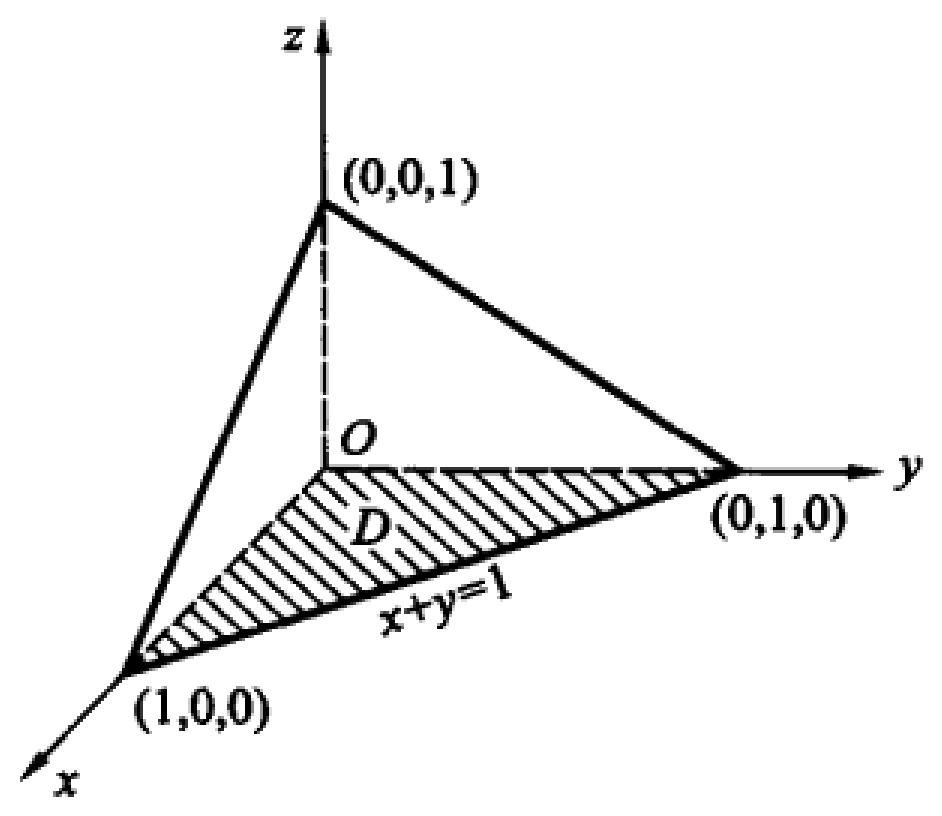
\includegraphics[width=0.5\textwidth]{work/figures/fig21-13}\caption{\relax}\label{fig:21-13}
\end{figure}

\begin{proof}[解法1]
曲面 $S$ 的方程为 $x+y+z=1$，它在 $xy$ 面上的投影为 $D$，由积分表达式的对称性及 $S$ 的对称性，有
\[
\begin{aligned}
I&=3\iint_{S}z\,\mathrm{d}x\mathrm{d}y=-3\iint_{D}(1-x-y)\,\mathrm{d}x\mathrm{d}y\\
&=-3\int_{0}^{1}\mathrm{d}x\int_{0}^{1-x}(1-x-y)\,\mathrm{d}y=-\frac{1}{2}.
\end{aligned}
\]
\end{proof}

\begin{proof}[解法2]
利用两种曲面积分的关系．因为曲面为 $x+y+z=1$ 的下侧，所以
\[
\bm{n}=-\frac{1}{\sqrt{3}}\{1,1,1\},
\]
\[
\begin{aligned}
I&=\iint_{S}x\,\mathrm{d}y\mathrm{d}z+y\,\mathrm{d}z\mathrm{d}x+z\,\mathrm{d}x\mathrm{d}y\\
&=-\frac{1}{\sqrt{3}}\iint_{S}(x+y+z)\,\mathrm{d}S=-\frac{1}{\sqrt{3}}\iint_{S}\mathrm{d}S\\
&=-\frac{1}{\sqrt{3}}\cdot\frac{1}{2}\cdot\sqrt{2}\cdot\sqrt{2}\sin\frac{\pi}{3}=-\frac{1}{2}.
\end{aligned}
\]
\end{proof}

\begin{example}\label{ex:21-4-2}
计算 $I=\displaystyle\iint_{S}x^{2}\,\mathrm{d}y\mathrm{d}z+y^{2}\,\mathrm{d}z\mathrm{d}x+z^{2}\,\mathrm{d}x\mathrm{d}y$，其中 $S$ 是半球面 $x^{2}+y^{2}+z^{2}=1$ $(z\geqslant0)$ 的上侧．
\end{example}

\begin{proof}[解]
对于 $\displaystyle\iint_{S}x^{2}\,\mathrm{d}y\mathrm{d}z$，将 $S$ 分为 $S_{1}$ 和 $S_{2}$ 两部分：

$S_{1}:x^{2}+y^{2}+z^{2}=1$ $(z\geqslant0,x\geqslant0)$ 前侧，

$S_{2}:x^{2}+y^{2}+z^{2}=1$ $(z\geqslant0,x\leqslant0)$ 后侧，

$S_{1}$，$S_{2}$ 在 $Oyz$ 面上的无向投影都是 $D$，故
\[
\begin{aligned}
\iint_{S}x^{2}\,\mathrm{d}y\mathrm{d}z&=\iint_{S_{1}}x^{2}\,\mathrm{d}y\mathrm{d}z+\iint_{S_{2}}x^{2}\,\mathrm{d}y\mathrm{d}z\\
&=\iint_{D}\left(1-y^{2}-z^{2}\right)\mathrm{d}y\mathrm{d}z-\iint_{D}\left(1-y^{2}-z^{2}\right)\mathrm{d}y\mathrm{d}z=0.
\end{aligned}
\]
由对称性立即可知，$\displaystyle\iint_{S}y^{2}\,\mathrm{d}z\mathrm{d}x=0$，而
\[
\begin{aligned}
\iint_{S}z^{2}\,\mathrm{d}x\mathrm{d}y&=\iint_{x^{2}+y^{2}\leqslant1}(1-x^{2}-y^{2})\,\mathrm{d}x\mathrm{d}y\\
&=\int_{0}^{2\pi}\mathrm{d}\theta\int_{0}^{1}(1-r^{2})r\,\mathrm{d}r=\frac{\pi}{2}.
\end{aligned}
\]
所以 $I=\dfrac{\pi}{2}$．
\end{proof}

\begin{figure}[htbp]
\centering
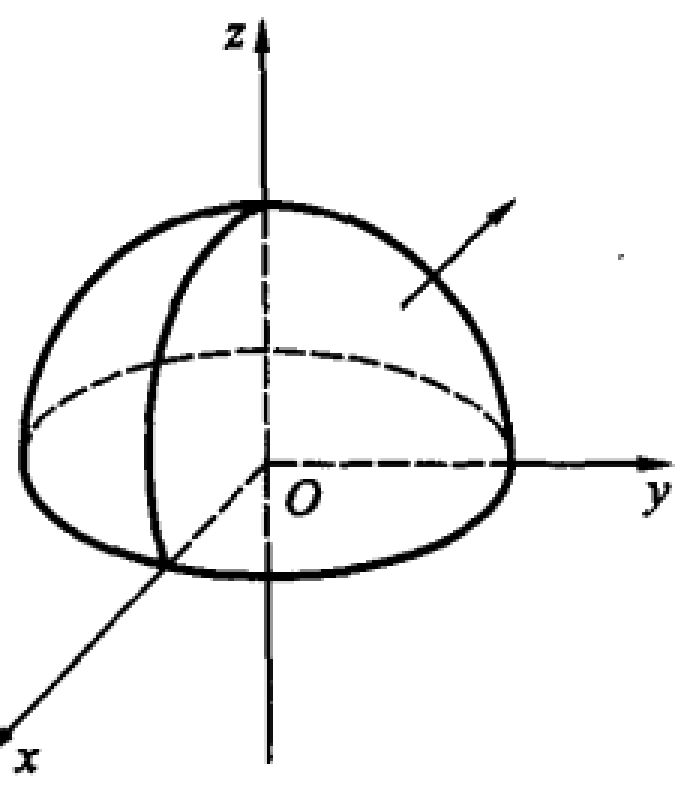
\includegraphics[width=0.45\textwidth]{work/figures/fig21-14}\caption{\relax}\label{fig:21-14}
\end{figure}

利用两种曲面积分之间的关系，我们立即可以导出 $S$ 由参数形式给出时的计算公式．设光滑曲面 $S$ 的参数方程为
\[
x=x(u,v),\quad y=y(u,v),\quad z=z(u,v),\quad(u,v)\in D
\]
则沿用前面的记号有
\[
\bm{n}=(\cos\alpha,\cos\beta,\cos\gamma)=\frac{\pm1}{\sqrt{A^{2}+B^{2}+C^{2}}}(A,B,C)
\]
因此
\[
\begin{aligned}
&\iint_{S}R(x,y,z)\,\mathrm{d}x\mathrm{d}y\\
={}&\iint_{S}R(x,y,z)\cos\gamma\,\mathrm{d}S\\
={}&\pm\iint_{D}R\big(x(u,v),y(u,v),z(u,v)\big)\,|C|\,\mathrm{d}u\mathrm{d}v\\
={}&\pm\iint_{D}R\big(x(u,v),y(u,v),z(u,v)\big)\left|\frac{\partial(x,y)}{\partial(u,v)}\right|\mathrm{d}u\mathrm{d}v,
\end{aligned}
\]
符号的选择为 $S$ 的上侧取正号，下侧取负号．

同理有
\[
\begin{aligned}
&\iint_{S}P(x,y,z)\,\mathrm{d}y\mathrm{d}z\\
={}&\pm\iint_{D}P\big(x(u,v),y(u,v),z(u,v)\big)\left|\frac{\partial(y,z)}{\partial(u,v)}\right|\mathrm{d}u\mathrm{d}v,
\end{aligned}
\]
符号的选择为 $S$ 的前侧取正号，后侧取负号．
\[
\begin{aligned}
&\iint_{S}Q(x,y,z)\,\mathrm{d}z\mathrm{d}x\\
={}&\pm\iint_{D}Q\big(x(u,v),y(u,v),z(u,v)\big)\left|\frac{\partial(z,x)}{\partial(u,v)}\right|\mathrm{d}u\mathrm{d}v,
\end{aligned}
\]
符号的选择为 $S$ 的右侧取正号，左侧取负号．

\begin{example}\label{ex:21-4-3}
求 $I=\displaystyle\iint_{S}x^{3}\,\mathrm{d}y\mathrm{d}z+y^{3}\,\mathrm{d}z\mathrm{d}x+z^{3}\,\mathrm{d}x\mathrm{d}y$，$S$ 是椭球面 $\dfrac{x^{2}}{a^{2}}+\dfrac{y^{2}}{b^{2}}+\dfrac{z^{2}}{c^{2}}=1$ 的外侧．
\end{example}

\begin{proof}[解]
$S$ 的参数方程为
\[
\begin{cases}
x=a\cos\theta\sin\varphi,\\
y=b\sin\theta\sin\varphi,\\
z=c\cos\varphi,
\end{cases}
\quad
\begin{aligned}
0&\leqslant\theta\leqslant2\pi,\\
0&\leqslant\varphi\leqslant\pi,
\end{aligned}
\]
\[
\frac{\partial(x,y)}{\partial(\varphi,\theta)}=\begin{vmatrix}a\cos\theta\cos\varphi&-a\sin\theta\sin\varphi\\ b\sin\theta\cos\varphi&b\cos\theta\sin\varphi\end{vmatrix}=ab\sin\varphi\cos\varphi.
\]
对于 $\displaystyle\iint_{S}z^{3}\,\mathrm{d}x\mathrm{d}y$，将 $S$ 分为上半椭球面 $S_{1}$ 的上侧和下半椭球面 $S_{2}$ 的下侧，则
\[
\begin{aligned}
&\iint_{S}z^{3}\,\mathrm{d}x\mathrm{d}y=\iint_{S_{1}}z^{3}\,\mathrm{d}x\mathrm{d}y+\iint_{S_{2}}z^{3}\,\mathrm{d}x\mathrm{d}y\\
&=\int_{0}^{2\pi}\mathrm{d}\theta\int_{0}^{\frac{\pi}{2}}(c\cos\varphi)^{3}\left|\frac{\partial(x,y)}{\partial(\varphi,\theta)}\right|\mathrm{d}\varphi-\int_{0}^{2\pi}\mathrm{d}\theta\int_{\frac{\pi}{2}}^{\pi}(c\cos\varphi)^{3}\left|\frac{\partial(x,y)}{\partial(\varphi,\theta)}\right|\mathrm{d}\varphi\\
&=2\pi abc^{3}\int_{0}^{\frac{\pi}{2}}\sin\varphi\cos^{4}\varphi\,\mathrm{d}\varphi+2\pi abc^{3}\int_{\frac{\pi}{2}}^{\pi}\cos^{4}\varphi\sin\varphi\,\mathrm{d}\varphi\\
&=4\pi abc^{3}\int_{0}^{\frac{\pi}{2}}\sin\varphi\cos^{4}\varphi\,\mathrm{d}\varphi=4\pi abc^{3}\,\frac{1}{5}\cos^{5}\varphi\,\Big|_{\frac{\pi}{2}}^{0}=\frac{4}{5}\pi abc^{3}.
\end{aligned}
\]
由对称性知
\[
\iint_{S}x^{3}\,\mathrm{d}y\mathrm{d}z=\frac{4}{5}\pi a^{3}bc,
\]
\[
\iint_{S}y^{3}\,\mathrm{d}z\mathrm{d}x=\frac{4}{5}\pi ab^{3}c,
\]
从而
\[
I=\frac{4}{5}\pi abc\left(a^{2}+b^{2}+c^{2}\right).
\]
\end{proof}

和第二型曲线积分类似，引入向量
\[
\begin{aligned}
\bm{F}(x,y,z)&=\left(P(x,y,z),Q(x,y,z),R(x,y,z)\right),\\
\mathrm{d}\bm{S}&=\bm{n}\cdot\mathrm{d}S=\left\{\cos\alpha,\cos\beta,\cos\gamma\right\}\mathrm{d}S\\
&=\left\{\mathrm{d}y\mathrm{d}z,\mathrm{d}z\mathrm{d}x,\mathrm{d}x\mathrm{d}y\right\},
\end{aligned}
\]
则
\[
\begin{aligned}
&\iint_{S}P\,\mathrm{d}y\mathrm{d}z+Q\,\mathrm{d}z\mathrm{d}x+R\,\mathrm{d}x\mathrm{d}y\\
={}&\iint_{S}\left(P\cos\alpha+Q\cos\beta+R\cos\gamma\right)\mathrm{d}S\\
={}&\iint_{S}\bm{F}\cdot\mathrm{d}\bm{S}.
\end{aligned}
\]
和曲线情形不同的是，这里 $\mathrm{d}\bm{S}$ 的方向为法线方向，与积分曲面 $S$ 的侧相同．

\begin{xiti}
\item 计算下列第二型曲线积分：
\begin{ziti}
\item $\displaystyle\int_{L}(2a-y)\,\mathrm{d}x+\mathrm{d}y$，其中 $L$ 为摆线 $x=a(t-\sin t)$，$y=a(1-\cos t)$ $(0\leqslant t\leqslant2\pi)$ 沿 $t$ 增加的方向；
\item $\displaystyle\int_{L}\dfrac{-x\,\mathrm{d}x+y\,\mathrm{d}y}{x^{2}+y^{2}}$，其中 $L$ 为圆周 $x^{2}+y^{2}=a^{2}$ 依逆时针方向；
\item $\displaystyle\int_{L}x\,\mathrm{d}x+y\,\mathrm{d}y+z\,\mathrm{d}z$，其中 $L$ 为从 $(1,1,1)$ 到 $(2,3,4)$ 的直线段；
\item $\displaystyle\int_{L}\left(x^{2}-2xy\right)\mathrm{d}x+\left(y^{2}-2xy\right)\mathrm{d}y$，$L$ 为 $y=x^{2}$ 从 $(1,1)$ 到 $(-1,1)$；
\item $\displaystyle\int_{L}y\,\mathrm{d}x-x\,\mathrm{d}y+\left(x^{2}+y^{2}\right)\mathrm{d}z$，$L$ 为曲线 $x=\mathrm{e}^{t}$，$y=\mathrm{e}^{-t}$，$z=at$ 从 $(1,1,0)$ 到 $\left(\mathrm{e},\mathrm{e}^{-1},a\right)$；
\item $\displaystyle\int_{L}\left(x^{2}+y^{2}\right)\mathrm{d}x+\left(x^{2}-y^{2}\right)\mathrm{d}y$，$L$ 为以 $A(1,0)$，$B(2,0)$，$C(2,1)$，$D(1,1)$ 为顶点的正方形沿逆时针方向．
\end{ziti}
\item 计算曲线积分
\[
\int_{L}\left(y^{2}-z^{2}\right)\mathrm{d}x+\left(z^{2}-x^{2}\right)\mathrm{d}y+\left(x^{2}-y^{2}\right)\mathrm{d}z.
\]
\begin{ziti}
\item $L$ 为球面三角形 $x^{2}+y^{2}+z^{2}=1$，$x\geqslant0$，$y\geqslant0$，$z\geqslant0$ 的边界线，从球的外侧看去，$L$ 的方向为逆时针方向；
\item $L$ 是球面 $x^{2}+y^{2}+z^{2}=a^{2}$ 和柱面 $x^{2}+y^{2}=ax$ $(a>0)$ 的交线位于 $Oxy$ 平面上方的部分，从 $x$ 轴上 $(b,0,0)$ $(b>a)$ 点看去，$L$ 是顺时针方向．
\end{ziti}
\item 求闭曲线 $L$ 上的第二型曲线积分
\[
\oint_{L}\dfrac{y\,\mathrm{d}x-x\,\mathrm{d}y}{x^{2}+y^{2}},
\]
\begin{ziti}
\item $L$ 为圆 $x^{2}+y^{2}=a^{2}$，逆时针方向；
\item $L$ 为椭圆 $\dfrac{x^{2}}{a^{2}}+\dfrac{y^{2}}{b^{2}}=1$，顺时针方向；
\item $L$ 为以 $(0,0)$ 为中心，边长为 $a$，对边平行于坐标轴的正方形，顺时针方向；
\item $L$ 是以 $(-1,-1)$，$(1,-1)$，$(0,1)$ 为顶点的三角形，顺时针方向．
\end{ziti}
\item 求力场 $\bm{F}$ 对运动的单位质点所作的功，此质点沿曲线 $L$ 从 $A$ 点运动到 $B$ 点：
\begin{ziti}
\item $\bm{F}=\left(x-2xy^{2},y-2x^{2}y\right)$，$L$ 为平面曲线 $y=x^{2}$，$A(0,0)$，$B(1,1)$；
\item $\bm{F}=(x+y,xy)$，$L$ 为平面曲线 $y=1-\left|1-x\right|$，$A(0,0)$，$B(2,0)$；
\item $\bm{F}=(x-y,y-z,z-x)$，$L$ 的矢量形式为 $\bm{r}(t)=t\bm{i}+t^{2}\bm{j}+t^{3}\bm{k}$，$A(0,0,0)$，$B(1,1,1)$；
\item $\bm{F}=\left(y^{2},z^{2},x^{2}\right)$，$L$ 的参数式为 $x=\alpha\cos t$，$y=\beta\sin t$，$z=\gamma t$ $(\alpha,\beta,\gamma$ 为正数)，$A(\alpha,0,0)$，$B(\alpha,0,2\pi\gamma)$．
\end{ziti}
\item 设 $P$，$Q$，$R$ 在 $L$ 上连续，$L$ 为光滑弧段，弧长为 $l$，证明
\[
\left|\int_{L}P\,\mathrm{d}x+Q\,\mathrm{d}y+R\,\mathrm{d}z\right|\leqslant Ml.
\]
其中 $M=\max\limits_{(x,y,z)\in L}\left\{\sqrt{P^{2}+Q^{2}+R^{2}}\right\}$．
\item 设光滑闭曲线 $L$ 在光滑曲面 $S$ 上，$S$ 的方程为 $z=f(x,y)$，曲线 $L$ 在 $Oxy$ 平面上的投影曲线为 $l$，函数 $P(x,y,z)$ 在 $L$ 上连续，证明：
\[
\oint_{L}P(x,y,z)\,\mathrm{d}x=\oint_{l}P(x,y,f(x,y))\,\mathrm{d}x.
\]
\item 计算 $I=\displaystyle\int_{L}xyz\,\mathrm{d}z$，其中 $L$ 为 $x^{2}+y^{2}+z^{2}=1$ 与 $y=z$ 相交的圆，其方向按曲线依次经过 $1$、$2$、$7$、$8$ 卦限．
\item 计算下列第二型曲面积分：
\begin{ziti}
\item $\displaystyle\iint_{S}y(x-z)\,\mathrm{d}y\mathrm{d}z+x^{2}\,\mathrm{d}z\mathrm{d}x+\left(y^{2}+xz\right)\mathrm{d}x\mathrm{d}y$，其中 $S$ 为 $x=y=z=0$，$x=y=z=a$ 六个平面所围的正立方体边界的外侧；
\item $\displaystyle\iint_{S}(x+y)\,\mathrm{d}y\mathrm{d}z+(y+z)\,\mathrm{d}z\mathrm{d}x+(z+x)\,\mathrm{d}x\mathrm{d}y$，其中 $S$ 是以原点为中心，边长为 $2$ 的正立方体表面的外侧；
\item $\displaystyle\iint_{S}yz\,\mathrm{d}z\mathrm{d}x$，$S$ 为 $\dfrac{x^{2}}{a^{2}}+\dfrac{y^{2}}{b^{2}}+\dfrac{z^{2}}{c^{2}}=1$ 的上半部分的上侧；
\item $\displaystyle\iint_{S}z\,\mathrm{d}x\mathrm{d}y+x\,\mathrm{d}y\mathrm{d}z+y\,\mathrm{d}z\mathrm{d}x$，$S$ 为柱面 $x^{2}+y^{2}=1$ 被平面 $z=0$ 及 $z=3$ 所截部分的外侧；
\item $\displaystyle\iint_{S}xy\,\mathrm{d}y\mathrm{d}z+yz\,\mathrm{d}z\mathrm{d}x+xz\,\mathrm{d}x\mathrm{d}y$，$S$ 是由平面 $x=y=z=0$ 和 $x+y+z=1$ 所围的四面体表面的外侧；
\item $\displaystyle\iint_{S}x^{3}\,\mathrm{d}y\mathrm{d}z+y^{3}\,\mathrm{d}z\mathrm{d}x+z^{3}\,\mathrm{d}x\mathrm{d}y$，$S$ 为球面 $x^{2}+y^{2}+z^{2}=a^{2}$ 的外侧；
\item $\displaystyle\iint_{S}x^{2}\,\mathrm{d}y\mathrm{d}z+y^{2}\,\mathrm{d}z\mathrm{d}x+z^{2}\,\mathrm{d}x\mathrm{d}y$，$S$ 是球面 $(x-a)^{2}+(y-b)^{2}+(z-c)^{2}=R^{2}$ 的外侧．
\end{ziti}
\item 设某流体的流速为 $\bm{v}=(k,y,0)$，求单位时间内从球面 $x^{2}+y^{2}+z^{2}=4$ 的内部流过球面的流量．
\item 设流体的流速为 $\bm{v}=\left(xy^{5},0,z^{5}x^{x}\right)$，求穿过柱面 $x^{2}+y^{2}=a^{2}$ $(-h\leqslant z\leqslant h)$ 外侧的流量．
\end{xiti}

% !TeX program = xelatex
% 第二十二章 各种积分间的联系与场论初步
\chapter{各种积分间的联系与场论初步}

本章给出联系二重积分与曲线积分、三重积分与曲面积分、空间曲面积分与曲线积分的重要公式，分别称为格林（G.\ Green，$1793$—$1841$）公式，高斯公式以及斯托克斯（G.\ Stokes，$1819$—$1903$）公式．它们可以看作牛顿－莱布尼茨公式的高维推广．场论是多元函数微积分学最重要应用的部分．本章还将给出上述三个公式在场论中的解释．本章的内容是为学习数学物理与近代分析准备必要的基础．

\section{各种积分间的联系}

\subsection{格林公式}

在讲这个公式以前，先介绍平面单连通区域的概念．

一个平面区域 $D$，如果全落在此区域内的任何一条封闭曲线都可以不经过 $D$ 以外的点而连续地收缩为属于 $D$ 的一点，则称 $D$ 为平面单连通区域．否则称为复连通区域．例如上半平面 $y\geqslant 0$ 是平面单连通区域，$x^{2}+y^{2}\leqslant 1$ 也是平面单连通区域，而 $x^{2}+y^{2}\geqslant 1$ 和 $0<x^{2}+y^{2}<1$ 都是复连通区域．可见，单连通区域就是不含有``洞''甚至``点洞''的区域（图~\ref{fig:22-1}），而复连通区域就是含有``洞''的区域（图~\ref{fig:22-2}）．

\begin{figure}[htbp]
\centering
\begin{minipage}[c]{0.42\textwidth}\centering
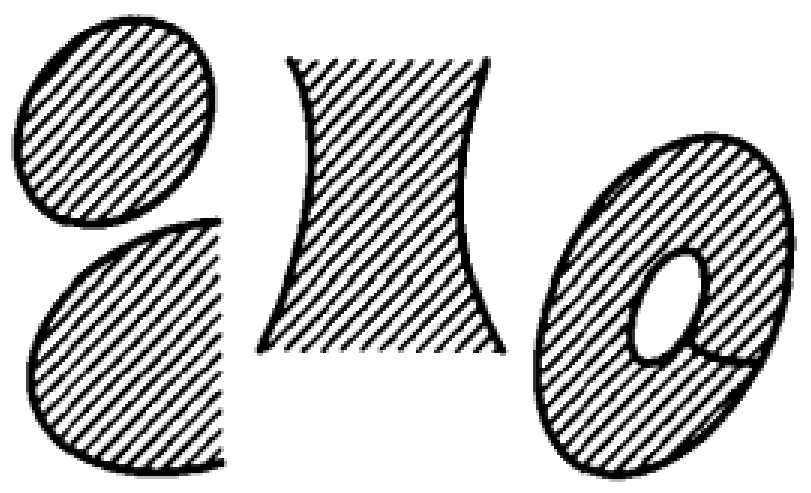
\includegraphics[width=\textwidth]{work/figures/fig22-1}\caption{\relax}\label{fig:22-1}
\end{minipage}\hfill
\begin{minipage}[c]{0.42\textwidth}\centering
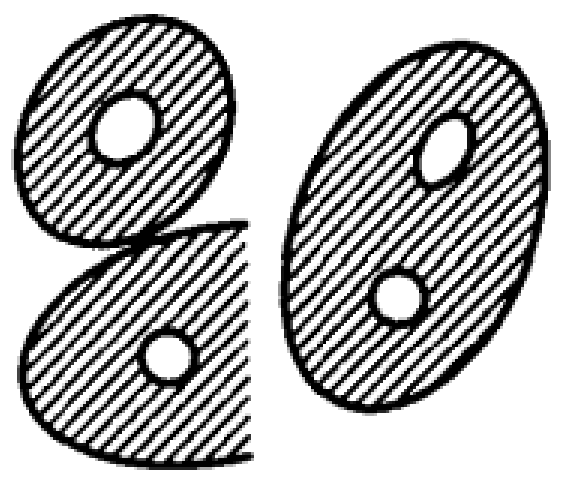
\includegraphics[width=\textwidth]{work/figures/fig22-2}\caption{\relax}\label{fig:22-2}
\end{minipage}
\end{figure}

\begin{theorem}[格林公式]\label{thm:22-1}
设 $D$ 是由逐段光滑闭曲线 $L$ 围成的平面单连通闭区域，函数 $P(x,y)$，$Q(x,y)$ 在 $D$ 上有一阶连续偏导数，则有
\begin{equation}\label{eq:green}
\iint_{D}\left(\frac{\partial Q}{\partial x}-\frac{\partial P}{\partial y}\right)\mathrm{d}x\mathrm{d}y=\oint_{L}P\mathrm{d}x+Q\mathrm{d}y, \tag{1}
\end{equation}
其中右端的积分路径是闭曲线 $L$，方向取正向．
\end{theorem}

回忆闭曲线正向的含义是，当一人沿曲线 $L$ 正向行走时，曲线 $L$ 所包围的区域 $D$ 恒在人的左边．

\begin{proof}
（1）先考虑区域是最简单的情形．设 $D$ 既可表为
\[
D=\left\{(x,y)\mid y_{1}(x)\leqslant y\leqslant y_{2}(x),\,a\leqslant x\leqslant b\right\},
\]
又可表为
\[
D=\left\{(x,y)\mid x_{1}(y)\leqslant x\leqslant x_{2}(y),\,c\leqslant y\leqslant d\right\}.
\]
即从上下来看，$D$ 由 $y=y_{2}(x)$ 与 $y=y_{1}(x)$（$a\leqslant x\leqslant b$）围成，而从左右来看，$D$ 是由 $x=x_{2}(y)$ 和 $x=x_{1}(y)$（$c\leqslant y\leqslant d$）围成（见图~\ref{fig:22-3}）．这时用牛顿－莱布尼茨公式和第二型曲线积分与定积分的关系，有
\begin{figure}[htbp]
\centering
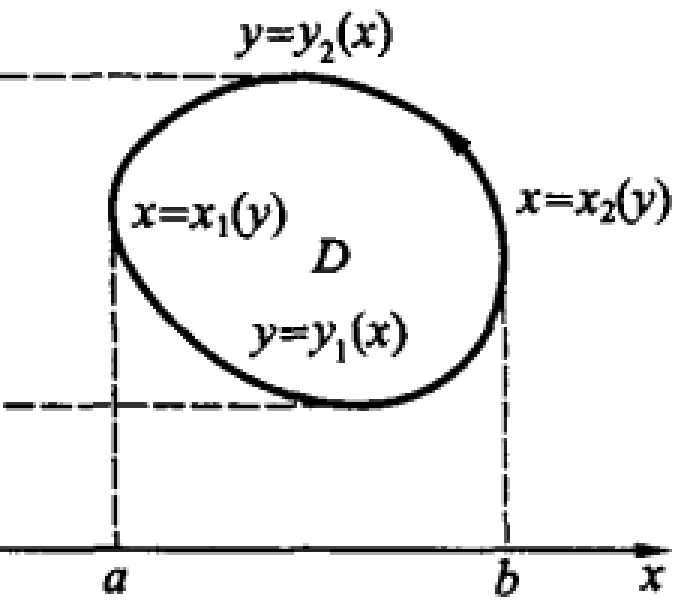
\includegraphics[width=0.30\textwidth]{work/figures/fig22-3}\caption{\relax}\label{fig:22-3}
\end{figure}
\[
\begin{aligned}
\iint_{D}\frac{\partial Q}{\partial x}\mathrm{d}x\mathrm{d}y&=\int_{c}^{d}\mathrm{d}y\int_{x_{1}(y)}^{x_{2}(y)}\frac{\partial Q}{\partial x}\mathrm{d}x\\
&=\int_{c}^{d}\left[Q\left(x_{2}(y),y\right)-Q\left(x_{1}(y),y\right)\right]\mathrm{d}y\\
&=\int_{L_{1}}Q(x,y)\mathrm{d}y+\int_{L_{2}}Q(x,y)\mathrm{d}y\\
&=\oint_{L}Q(x,y)\mathrm{d}y.
\end{aligned}
\]
其中 $\displaystyle\int_{L_{1}}$ 与 $\displaystyle\int_{L_{2}}$ 分别表示沿右边的曲线 $x=x_{2}(y)$ 与左边的曲线 $x=x_{1}(y)$ 按 $L$ 的方向的第二型曲线积分．同理
\[
\begin{aligned}
\iint_{D}\frac{\partial P}{\partial y}\mathrm{d}x\mathrm{d}y&=\int_{a}^{b}\mathrm{d}x\int_{y_{1}(x)}^{y_{2}(x)}\frac{\partial P}{\partial y}\mathrm{d}y\\
&=\int_{a}^{b}\left[P\left(x,y_{2}(x)\right)-P\left(x,y_{1}(x)\right)\right]\mathrm{d}x\\
&=-\oint_{L}P(x,y)\mathrm{d}x.
\end{aligned}
\]
因此
\[
\iint_{D}\left(\frac{\partial Q}{\partial x}-\frac{\partial P}{\partial y}\right)\mathrm{d}x\mathrm{d}y=\oint_{L}P(x,y)\mathrm{d}x+Q(x,y)\mathrm{d}y.
\]
（2）如果区域如图~\ref{fig:22-4}，则公式\eqref{eq:green}仍然成立．事实上，这时\eqref{eq:green}的证明对 $\displaystyle\iint_{D}\frac{\partial Q}{\partial x}\mathrm{d}x\mathrm{d}y$
\begin{figure}[htbp]
\centering
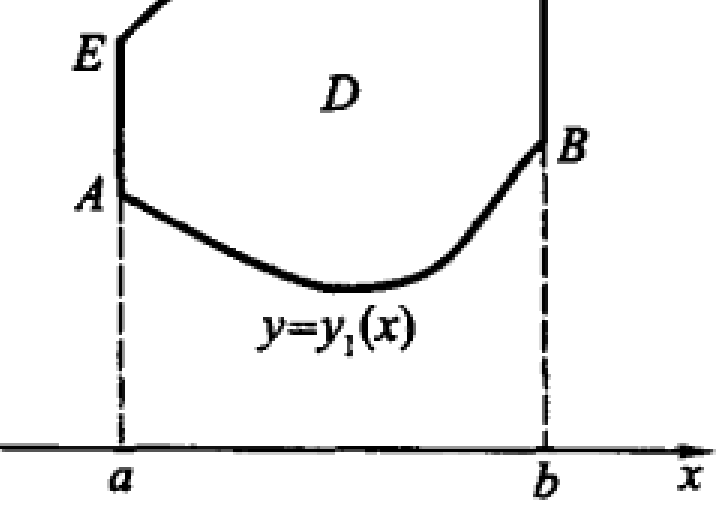
\includegraphics[width=0.30\textwidth]{work/figures/fig22-4}\caption{\relax}\label{fig:22-4}
\end{figure}
完全适用．对另一项的证明需稍作修改．
\[
\begin{aligned}
\iint_{D}\frac{\partial P}{\partial y}\mathrm{d}x\mathrm{d}y&=\int_{a}^{b}\mathrm{d}x\int_{y_{1}(x)}^{y_{2}(x)}\frac{\partial P}{\partial y}\mathrm{d}y\\
&=\int_{a}^{b}\left[P\left(x,y_{2}(x)\right)-P\left(x,y_{1}(x)\right)\right]\mathrm{d}x\\
&=-\left[\int_{\widehat{AB}}P(x,y)\mathrm{d}x+\int_{\widehat{CE}}P(x,y)\mathrm{d}x\right].
\end{aligned}
\]
注意到 $\widehat{BC}$ 与 $\widehat{EA}$ 是两条平行于 $y$ 轴的直线，根据第二型曲线积分的定义，必然有
\[
\int_{\widehat{BC}}P(x,y)\mathrm{d}x=\int_{\widehat{EA}}P(x,y)\mathrm{d}x=0.
\]
把它们加到上面等式的右边，便得
\[
\begin{aligned}
\iint_{D}\frac{\partial P}{\partial y}\mathrm{d}x\mathrm{d}y&=-\left(\int_{\widehat{AB}}P\,\mathrm{d}x+\int_{\widehat{BC}}P\,\mathrm{d}x+\int_{\widehat{CE}}P\,\mathrm{d}x+\int_{\widehat{EA}}P\,\mathrm{d}x\right)\\
&=-\oint_{L}P(x,y)\mathrm{d}x,
\end{aligned}
\]
这样便证明了公式\eqref{eq:green}成立．

同理，对如图~\ref{fig:22-5} 的区域 $D$，公式也是成立的．
\begin{figure}[htbp]
\centering
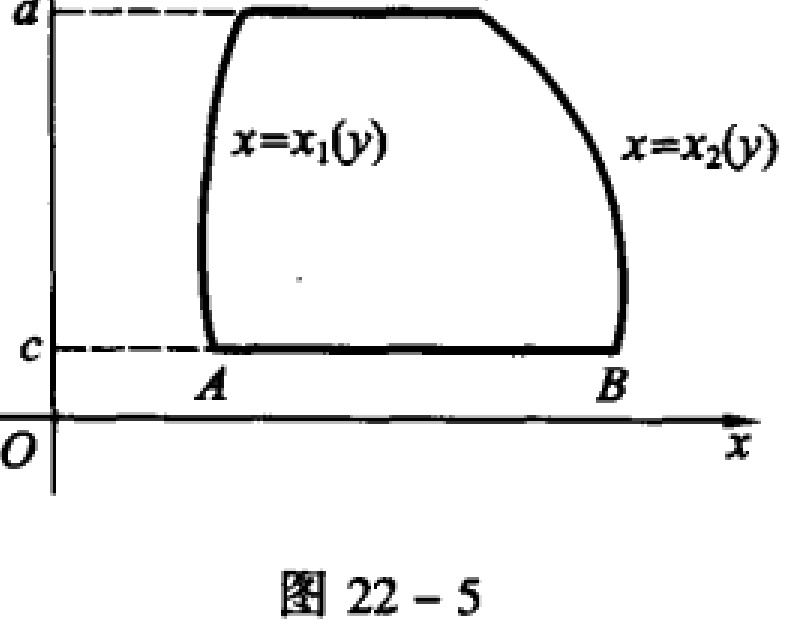
\includegraphics[width=0.30\textwidth]{work/figures/fig22-5}\caption{\relax}\label{fig:22-5}
\end{figure}

（3）如果区域可用若干条光滑曲线分成有限个（1）或（2）中讨论过的区域，则公式仍然成立．事实上，例如图~\ref{fig:22-6}，用直线段 $AB$ 把 $D$ 分成三个（2）讨论过的区域 $D_{1}$、$D_{2}$ 和 $D_{3}$．利用（2）中已证的结果，有
\begin{figure}[htbp]
\centering
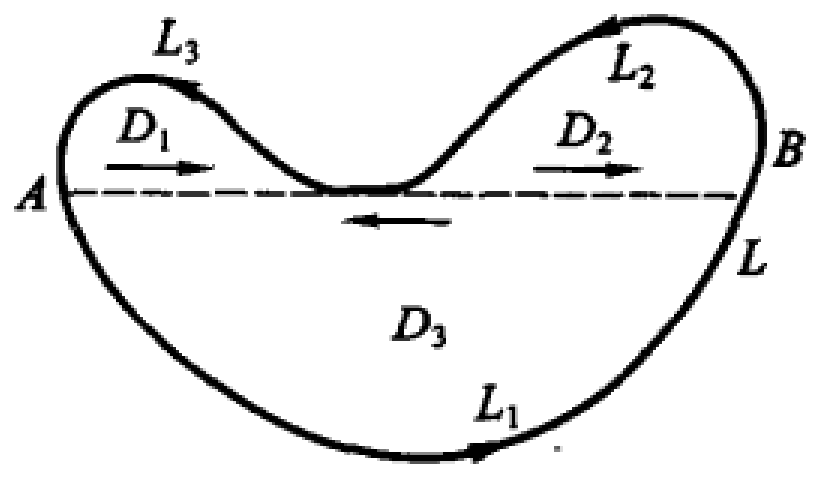
\includegraphics[width=0.30\textwidth]{work/figures/fig22-6}\caption{\relax}\label{fig:22-6}
\end{figure}
\[
\begin{aligned}
\iint_{D}\left(\frac{\partial Q}{\partial x}-\frac{\partial P}{\partial y}\right)\mathrm{d}x\mathrm{d}y&=\sum_{i=1}^{3}\iint_{D_{i}}\left(\frac{\partial Q}{\partial x}-\frac{\partial P}{\partial y}\right)\mathrm{d}x\mathrm{d}y\\
&=\sum_{i=1}^{3}\int_{L_{i}}P\mathrm{d}x+Q\mathrm{d}y\\
&=\oint_{L}P\mathrm{d}x+Q\mathrm{d}y,
\end{aligned}
\]
最后一个等式成立是因为沿直线 $AB$ 的两个不同方向各积分了一次，因此相应项积分的和为零．定理~\ref{thm:22-1} 证完．
\end{proof}

其实，对复连通区域，公式也是成立的，如图~\ref{fig:22-7}，我们用两条直线段 $AB$ 与 $CE$ 把复连通区域 $D$ 分成两个前面讨论过的区域 $D_{1}$、$D_{2}$，分别对 $D_{1}$、$D_{2}$ 用公式，便得到
\begin{figure}[htbp]
\centering
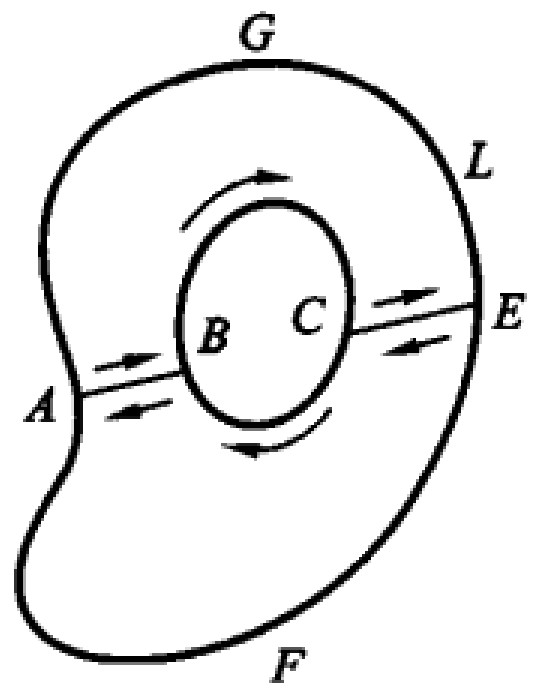
\includegraphics[width=0.22\textwidth]{work/figures/fig22-7}\caption{\relax}\label{fig:22-7}
\end{figure}
\[
\begin{aligned}
\iint_{D}\left(\frac{\partial Q}{\partial x}-\frac{\partial P}{\partial y}\right)\mathrm{d}x\mathrm{d}y&=\left(\iint_{D_{1}}+\iint_{D_{2}}\right)\left(\frac{\partial Q}{\partial x}-\frac{\partial P}{\partial y}\right)\mathrm{d}x\mathrm{d}y\\
&=\left(\int_{\widehat{ABCEGA}}+\int_{\widehat{AFECBA}}\right)P\mathrm{d}x+Q\mathrm{d}y\\
&=\oint_{L}P\mathrm{d}x+Q\mathrm{d}y,
\end{aligned}
\]
其中 $L$ 分别表示在两条闭曲线上的积分：一条沿外面的曲线按逆时针方向，一条沿内部的曲线按顺时针方向，加起来正是沿 $D$ 的全部边界 $L$ 作线积分，方向取正向：当人沿 $L$ 走时，区域 $D$ 永远在人的左边．而在推导过程中，沿 $\widehat{AB}$，$\widehat{CE}$ 的积分也是按不同方向各积分了一次，因此其和抵消而在最终结果中不出现．

对多于一个``洞''的复连通区域可类似处理．

为了便于记忆，格林公式可以写成如下的形式：
\[
\iint_{D}\begin{vmatrix}\dfrac{\partial}{\partial x}&\dfrac{\partial}{\partial y}\\[4pt] P&Q\end{vmatrix}\mathrm{d}x\mathrm{d}y=\oint_{L}P\mathrm{d}x+Q\mathrm{d}y.
\]
牛顿－莱布尼茨公式的一种解释是，它建立了函数在一个区间的定积分与其原函数在区间边界（两个点）的值之间的联系．格林公式给出了二元函数在平面区域的重积分与其``原函数''在区域边界的第二型曲线积分间的联系．从这个意义上说，格林公式可以看作牛顿－莱布尼茨公式的二维推广．

可以应用格林公式计算某些曲线积分．

\begin{example}\label{ex:22-1-1}
求 $\displaystyle\int_{\widehat{AMO}}\left(\mathrm{e}^{x}\sin y-my\right)\mathrm{d}x+\left(\mathrm{e}^{x}\cos y-m\right)\mathrm{d}y$，其中 $\widehat{AMO}$ 为由 $A(a,0)$ 至 $O(0,0)$，经上半圆周 $x^{2}+y^{2}=ax$ 的道路（图~\ref{fig:22-8}）．
\end{example}

\begin{proof}[解]
$\widehat{AMO}$ 不是封闭曲线，如果加上直线段 $\widehat{OA}$ 则构成封闭曲线 $L$．注意到沿 $\widehat{OA}$，函数 $\mathrm{e}^{x}\sin y-my$ 为 $0$，且 $\widehat{OA}$ 在 $y$ 轴上的投影为一点，因此
\[
\int_{\widehat{OA}}\left(\mathrm{e}^{x}\sin y-my\right)\mathrm{d}x+\left(\mathrm{e}^{x}\cos y-m\right)\mathrm{d}y=0.
\]
\begin{figure}[htbp]
\centering
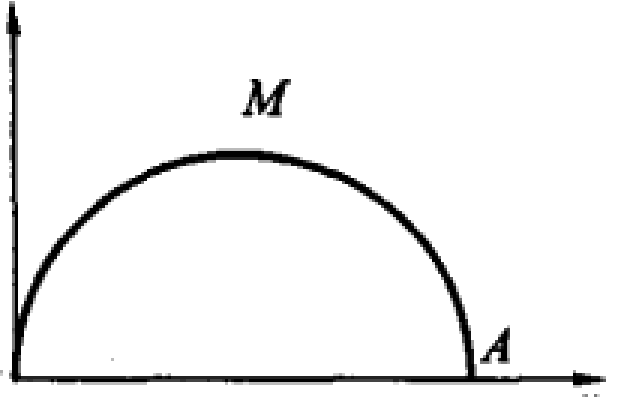
\includegraphics[width=0.26\textwidth]{work/figures/fig22-8}\caption{\relax}\label{fig:22-8}
\end{figure}
故添上 $\widehat{OA}$ 后用格林公式得
\[
\begin{aligned}
&\int_{\widehat{AMO}}\left(\mathrm{e}^{x}\sin y-my\right)\mathrm{d}x+\left(\mathrm{e}^{x}\cos y-m\right)\mathrm{d}y\\
=&\oint_{L}\left(\mathrm{e}^{x}\sin y-my\right)\mathrm{d}x+\left(\mathrm{e}^{x}\cos y-m\right)\mathrm{d}y\\
=&\iint_{D}\left(\mathrm{e}^{x}\cos y-\mathrm{e}^{x}\cos y+m\right)\mathrm{d}x\mathrm{d}y\\
=&m\iint_{D}\mathrm{d}x\mathrm{d}y=m\cdot\frac{1}{2}\pi\left(\frac{a}{2}\right)^{2}=\frac{m}{8}\pi a^{2}.
\end{aligned}
\]
\end{proof}

\begin{example}\label{ex:22-1-2}
计算 $I=\displaystyle\oint_{L}\frac{x\mathrm{d}y-y\mathrm{d}x}{x^{2}+y^{2}}$，其中 $L$ 为 $x^{2}+y^{2}=a^{2}$ 的正向．
\end{example}

\begin{proof}[解]
在 $L$ 上有 $x^{2}+y^{2}=a^{2}$，故有
\[
I=\frac{1}{a^{2}}\oint_{L}x\mathrm{d}y-y\mathrm{d}x.
\]
取 $P(x,y)=-y$，$Q(x,y)=x$，由格林公式得
\[
I=\frac{1}{a^{2}}\iint_{D}2\mathrm{d}x\mathrm{d}y=\frac{2}{a^{2}}\pi a^{2}=2\pi.
\]
\end{proof}

请读者思考，可否对 $P(x,y)=\dfrac{-y}{x^{2}+y^{2}}$，$Q(x,y)=\dfrac{x}{x^{2}+y^{2}}$ 直接用格林公式．为什么？

在例~\ref{ex:22-1-2} 中我们还看到平面区域 $D$ 的面积可以用第二型曲线积分表示为
\[
|D|=\iint_{D}\mathrm{d}x\mathrm{d}y=\frac{1}{2}\oint_{L}x\mathrm{d}y-y\mathrm{d}x.
\]
这是我们在本教程上册第八章 §2 推导过、在第二十章 §3 重积分变量代换中应用过的公式．

\begin{example}\label{ex:22-1-3}
求星形线 $x=a\cos^{3}t$，$y=b\sin^{3}t$（$0\leqslant t\leqslant 2\pi$）所围区域的面积．
\end{example}

\begin{proof}[解]
\[
\begin{aligned}
|D|&=\frac{1}{2}\oint_{L}x\mathrm{d}y-y\mathrm{d}x\\
&=\frac{1}{2}\int_{0}^{2\pi}\left[a\cos^{3}t\cdot 3b\sin^{2}t\cos t+b\sin^{3}t\cdot 3a\cos^{2}t\sin t\right]\mathrm{d}t\\
&=\frac{3}{2}ab\int_{0}^{2\pi}\sin^{2}t\cos^{2}t\,\mathrm{d}t=6ab\int_{0}^{\frac{\pi}{2}}\left(\sin^{2}t-\sin^{4}t\right)\mathrm{d}t\\
&=6ab\left(\frac{1}{2}-\frac{3\cdot 1}{4\cdot 2}\right)\frac{\pi}{2}=\frac{3}{8}\pi ab.
\end{aligned}
\]
\end{proof}

\subsection{高斯公式}

\begin{theorem}[高斯公式]\label{thm:22-2}
设空间区域 $V$ 由分片光滑的双侧封闭曲面 $S$ 围成，函数 $P(x,y,z)$，$Q(x,y,z)$，$R(x,y,z)$ 在 $V$ 及 $S$ 上有一阶连续偏导数，则有
\[
\iiint_{V}\left(\frac{\partial P}{\partial x}+\frac{\partial Q}{\partial y}+\frac{\partial R}{\partial z}\right)\mathrm{d}x\mathrm{d}y\mathrm{d}z=\oiint_{S}P\mathrm{d}y\mathrm{d}z+Q\mathrm{d}z\mathrm{d}x+R\mathrm{d}x\mathrm{d}y,
\]
其中 $S$ 的方向为外侧．
\end{theorem}

\begin{proof}
仿照格林公式的证明，先对简单的区域证明高斯公式．考虑
\[
\iiint_{V}\frac{\partial R}{\partial z}\mathrm{d}x\mathrm{d}y\mathrm{d}z=\oiint_{S}R\mathrm{d}x\mathrm{d}y,
\]
其中 $V$ 如图~\ref{fig:22-9}，它的边界由下、上、中三部分 $S_{1}$、$S_{2}$、$S_{3}$ 构成．上部为 $S_{2}$，由方程 $z=z_{2}(x,y)$ 给出，下部为 $S_{1}$，由方程 $z=z_{1}(x,y)$ 给出，中间由母线平行于 $z$ 轴的柱面 $S_{3}$ 构成．$S_{1}$ 与 $S_{2}$ 在 $Oxy$ 平面上有公共投影 $D$．$V$ 可表为
\[
V=\{(x,y,z)\mid z_{1}(x,y)\leqslant z\leqslant z_{2}(x,y),(x,y)\in D\}.
\]
$V$ 的边界曲面 $S$ 的外侧可表为
\[
\begin{aligned}
S_{1}:&\ z=z_{1}(x,y),(x,y)\in D,\ \text{下侧},\\
S_{2}:&\ z=z_{2}(x,y),(x,y)\in D,\ \text{上侧},\\
S_{3}:&\ \text{以}\ D\ \text{的边界为准线夹在}\ S_{1}\ \text{与}\ S_{2}\ \text{之间的柱面外侧}.
\end{aligned}
\]
\begin{figure}[htbp]
\centering
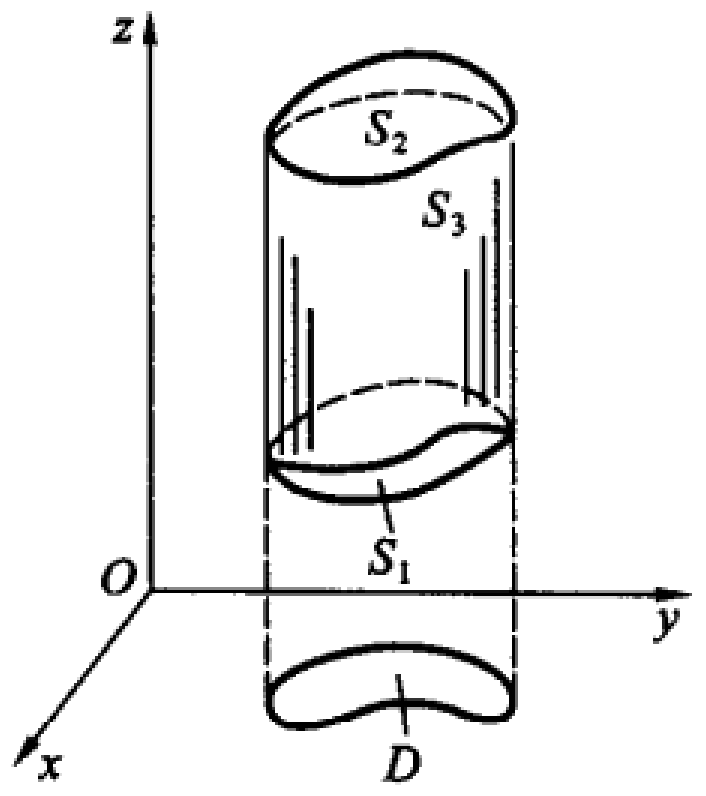
\includegraphics[width=0.28\textwidth]{work/figures/fig22-9}\caption{\relax}\label{fig:22-9}
\end{figure}
由三重积分的计算方法及第二型曲面积分的计算方法得
\[
\begin{aligned}
\iiint_{V}\frac{\partial R}{\partial z}\mathrm{d}x\mathrm{d}y\mathrm{d}z&=\iint_{D}\mathrm{d}x\mathrm{d}y\int_{z_{1}(x,y)}^{z_{2}(x,y)}\frac{\partial R}{\partial z}\mathrm{d}z\\
&=\iint_{D_{xy}}\left[R\left(x,y,z_{2}(x,y)\right)-R\left(x,y,z_{1}(x,y)\right)\right]\mathrm{d}x\mathrm{d}y\\
&=\iint_{S_{2}}R(x,y,z)\mathrm{d}x\mathrm{d}y+\iint_{S_{1}}R(x,y,z)\mathrm{d}x\mathrm{d}y\\
&=\left(\iint_{S_{1}}+\iint_{S_{2}}+\iint_{S_{3}}\right)R(x,y,z)\mathrm{d}x\mathrm{d}y\\
&=\oiint_{S}R(x,y,z)\mathrm{d}x\mathrm{d}y.
\end{aligned}
\]
上面第四个等式成立是因为 $S_{3}$ 在 $Oxy$ 面上的投影面积为零，所以
\[
\iint_{S_{3}}R(x,y,z)\mathrm{d}x\mathrm{d}y=0.
\]
同理可证
\[
\iiint_{V}\frac{\partial P}{\partial x}\mathrm{d}x\mathrm{d}y\mathrm{d}z=\oiint_{S}P\mathrm{d}y\mathrm{d}z,\qquad
\iiint_{V}\frac{\partial Q}{\partial y}\mathrm{d}x\mathrm{d}y\mathrm{d}z=\oiint_{S}Q\mathrm{d}z\mathrm{d}x.
\]
对于一般的区域 $V$，可以通过添加有限块光滑曲面，把它分为有限个上面已证明过的简单子区域的并．例如对图~\ref{fig:22-10} 和图~\ref{fig:22-11} 中的区域，高斯公式仍成立．完全类似于格林公式的推导，对每个子区域分别用高斯公式然后相加，注意到在添加的曲面上，恰好对不同的两侧各积分了一次，因而互相抵消，从而在曲面积分中不出现这些添加的曲面．定理~\ref{thm:22-2} 证完．
\end{proof}

\begin{figure}[htbp]
\centering
\begin{minipage}[c]{0.42\textwidth}\centering
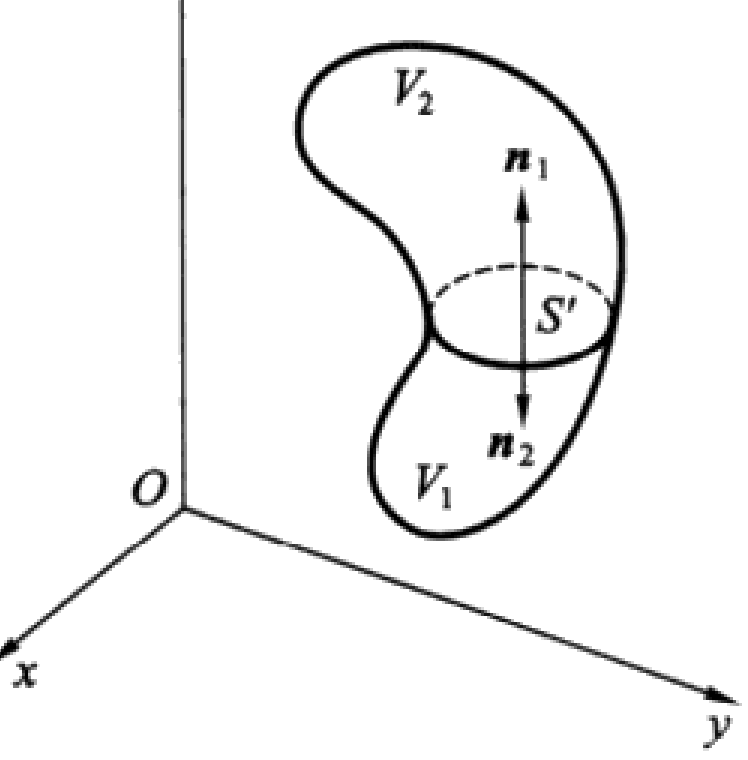
\includegraphics[width=\textwidth]{work/figures/fig22-10}\caption{\relax}\label{fig:22-10}
\end{minipage}\hfill
\begin{minipage}[c]{0.42\textwidth}\centering
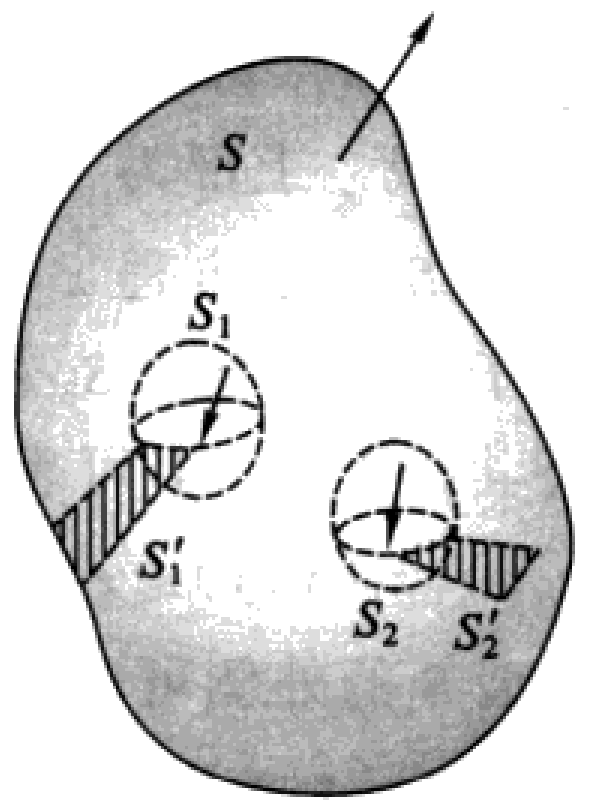
\includegraphics[width=\textwidth]{work/figures/fig22-11}\caption{\relax}\label{fig:22-11}
\end{minipage}
\end{figure}

利用两种曲面积分之间的关系，不难得到高斯公式的另一种形式
\[
\iiint_{V}\left(\frac{\partial P}{\partial x}+\frac{\partial Q}{\partial y}+\frac{\partial R}{\partial z}\right)\mathrm{d}x\mathrm{d}y\mathrm{d}z=\oiint_{S}\left(P\cos\alpha+Q\cos\beta+R\cos\gamma\right)\mathrm{d}S,
\]
其中 $\bm{n}=(\cos\alpha,\cos\beta,\cos\gamma)$ 是 $S$ 指向 $V$ 的外部的单位法向量．

高斯公式给出了函数在三维区域上的重积分与其``原函数''在区域边界上的第二型曲面积分间的联系，在这个意义上说，高斯公式是牛顿－莱布尼茨公式的三维推广．

\begin{example}\label{ex:22-1-4}
计算 $I=\displaystyle\oiint_{S}\frac{1}{x^{2}+y^{2}+z^{2}}\left(x^{3}\mathrm{d}y\mathrm{d}z+y^{3}\mathrm{d}z\mathrm{d}x+z^{3}\mathrm{d}x\mathrm{d}y\right)$，其中 $S$ 是 $x^{2}+y^{2}+z^{2}=a^{2}$ 的外侧．
\end{example}

\begin{proof}[解]
因为在 $S$ 上有 $x^{2}+y^{2}+z^{2}=a^{2}$，故
\[
I=\frac{1}{a^{2}}\oiint_{S}x^{3}\mathrm{d}y\mathrm{d}z+y^{3}\mathrm{d}z\mathrm{d}x+z^{3}\mathrm{d}x\mathrm{d}y.
\]
由高斯公式
\[
\begin{aligned}
I&=\frac{3}{a^{2}}\iiint_{V}\left(x^{2}+y^{2}+z^{2}\right)\mathrm{d}x\mathrm{d}y\mathrm{d}z\\
&=\frac{3}{a^{2}}\int_{0}^{2\pi}\mathrm{d}\theta\int_{0}^{\pi}\mathrm{d}\varphi\int_{0}^{a}r^{4}\sin\varphi\,\mathrm{d}r\\
&=\frac{12}{5}\pi a^{3}.
\end{aligned}
\]
\end{proof}

请读者思考，可否对 $P=\dfrac{x^{3}}{x^{2}+y^{2}+z^{2}}$，$Q=\dfrac{y^{3}}{x^{2}+y^{2}+z^{2}}$，$R=\dfrac{z^{3}}{x^{2}+y^{2}+z^{2}}$ 直接用高斯公式．另一个问题是为什么
\[
\iiint_{V}\left(x^{2}+y^{2}+z^{2}\right)\mathrm{d}x\mathrm{d}y\mathrm{d}z\neq a^{2}\iiint_{V}\mathrm{d}x\mathrm{d}y\mathrm{d}z.
\]

\subsection{斯托克斯公式}

\begin{theorem}[斯托克斯公式]\label{thm:22-3}
若光滑曲面 $S$ 的边界为光滑曲线 $L$，函数 $P$、$Q$、$R$ 在曲面 $S$ 及曲线 $L$ 上具有连续的一阶偏导数，则
\[
\begin{aligned}
&\iint_{S}\left(\frac{\partial R}{\partial y}-\frac{\partial Q}{\partial z}\right)\mathrm{d}y\mathrm{d}z+\left(\frac{\partial P}{\partial z}-\frac{\partial R}{\partial x}\right)\mathrm{d}z\mathrm{d}x+\left(\frac{\partial Q}{\partial x}-\frac{\partial P}{\partial y}\right)\mathrm{d}x\mathrm{d}y\\
&=\oint_{L}P\mathrm{d}x+Q\mathrm{d}y+R\mathrm{d}z,
\end{aligned}
\]
其中 $S$ 的侧与 $L$ 的方向按右手法则确定，即若四个手指的方向为 $L$ 的方向，则大拇指所指的方向就是曲面 $S$ 的方向，如图~\ref{fig:22-13}．
\end{theorem}

\begin{figure}[htbp]
\centering
\begin{minipage}[c]{0.46\textwidth}\centering
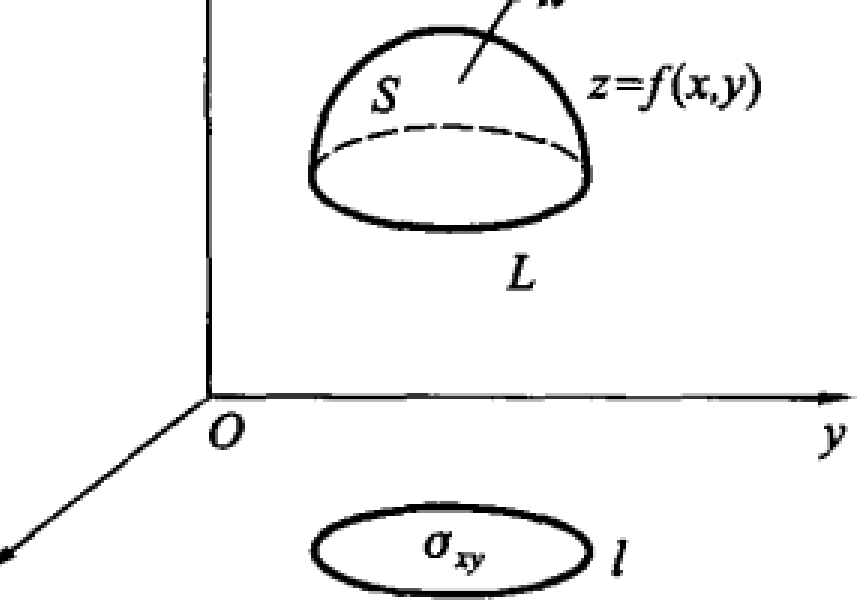
\includegraphics[width=\textwidth]{work/figures/fig22-12}\caption{\relax}\label{fig:22-12}
\end{minipage}\hfill
\begin{minipage}[c]{0.34\textwidth}\centering
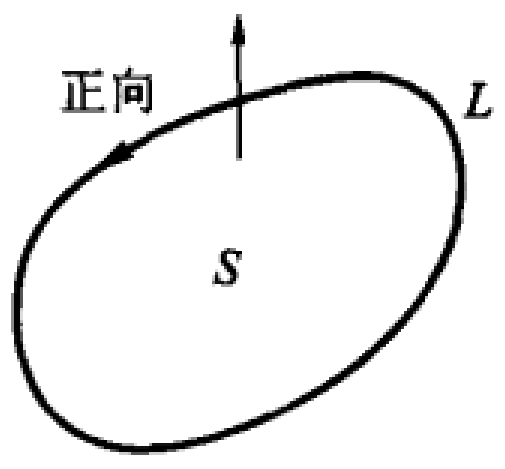
\includegraphics[width=\textwidth]{work/figures/fig22-13}\caption{\relax}\label{fig:22-13}
\end{minipage}
\end{figure}

\begin{proof}
先证
\[
\iint_{S}\frac{\partial P}{\partial z}\mathrm{d}z\mathrm{d}x-\frac{\partial P}{\partial y}\mathrm{d}x\mathrm{d}y=\oint_{L}P\mathrm{d}x.
\]
设曲面 $S$ 的方程为 $z=f(x,y)$，它在 $Oxy$ 面上的投影为 $\sigma_{xy}$，与过 $\sigma_{xy}$ 的点且平行于 $z$ 轴的直线只交于一点．$L$ 是 $S$ 的边界，它在 $Oxy$ 面上的投影为 $l$．取 $S$ 的上侧为正侧，则单位法向量为
\[
\bm{n}=(\cos\alpha,\cos\beta,\cos\gamma)=\frac{1}{\sqrt{\left(\dfrac{\partial z}{\partial x}\right)^{2}+\left(\dfrac{\partial z}{\partial y}\right)^{2}+1}}\left(-\frac{\partial z}{\partial x},-\frac{\partial z}{\partial y},1\right).
\]
因此
\[
\frac{\partial z}{\partial x}=-\frac{\cos\alpha}{\cos\gamma},\quad\frac{\partial z}{\partial y}=-\frac{\cos\beta}{\cos\gamma}.
\]
因为 $L$ 在曲面 $z=f(x,y)$ 上，所以由格林公式，有
\[
\begin{aligned}
\oint_{L}P(x,y,z)\mathrm{d}x&=\oint_{l}P(x,y,z(x,y))\mathrm{d}x\\
&=-\iint_{\sigma_{xy}}\left(\frac{\partial P}{\partial y}+\frac{\partial P}{\partial z}\frac{\partial z}{\partial y}\right)\mathrm{d}x\mathrm{d}y\\
&=-\iint_{\sigma_{xy}}\left(\frac{\partial P}{\partial y}-\frac{\partial P}{\partial z}\frac{\cos\beta}{\cos\gamma}\right)\mathrm{d}x\mathrm{d}y\\
&=\iint_{\sigma_{xy}}\left(\frac{\partial P}{\partial z}\cos\beta-\frac{\partial P}{\partial y}\cos\gamma\right)\frac{\mathrm{d}x\mathrm{d}y}{\cos\gamma}\\
&=\iint_{S}\left(\frac{\partial P}{\partial z}\cos\beta-\frac{\partial P}{\partial y}\cos\gamma\right)\mathrm{d}S\\
&=\iint_{S}\frac{\partial P}{\partial z}\mathrm{d}z\mathrm{d}x-\frac{\partial P}{\partial y}\mathrm{d}x\mathrm{d}y.
\end{aligned}
\]
同理可证
\[
\oint_{L}Q\mathrm{d}y=\iint_{S}\frac{\partial Q}{\partial x}\mathrm{d}x\mathrm{d}y-\frac{\partial Q}{\partial z}\mathrm{d}y\mathrm{d}z,
\]
\[
\oint_{L}R\mathrm{d}z=\iint_{S}\frac{\partial R}{\partial y}\mathrm{d}y\mathrm{d}z-\frac{\partial R}{\partial x}\mathrm{d}z\mathrm{d}x.
\]
把三个式子加起来，便得斯托克斯公式．定理~\ref{thm:22-3} 证完．
\end{proof}

斯托克斯公式建立了函数在空间曲面 $S$ 上的第二型曲面积分与其``原函数''在 $S$ 的边界曲线 $L$ 上的第二型曲线积分之间的联系，因此也是牛顿－莱布尼茨公式的一种高维的推广．利用两种曲面积分之间的关系，常把它写成如下便于记忆的形式：
\[
\begin{aligned}
\oint_{L}P\mathrm{d}x+Q\mathrm{d}y+R\mathrm{d}z&=\iint_{S}\begin{vmatrix}\mathrm{d}y\mathrm{d}z&\mathrm{d}z\mathrm{d}x&\mathrm{d}x\mathrm{d}y\\[3pt]\dfrac{\partial}{\partial x}&\dfrac{\partial}{\partial y}&\dfrac{\partial}{\partial z}\\[3pt] P&Q&R\end{vmatrix}\\
&=\iint_{S}\begin{vmatrix}\cos\alpha&\cos\beta&\cos\gamma\\[3pt]\dfrac{\partial}{\partial x}&\dfrac{\partial}{\partial y}&\dfrac{\partial}{\partial z}\\[3pt] P&Q&R\end{vmatrix}\mathrm{d}S.
\end{aligned}
\]
不难看出，格林公式是斯托克斯公式的特殊情形．当 $L$ 是 $Oxy$ 平面上的闭曲线时，$\mathrm{d}z=0$．取 $S$ 为 $Oxy$ 面上由 $L$ 围成的区域，则 $S$ 在 $Oyz$ 和 $Ozx$ 平面上的投影为零，因此对 $\mathrm{d}y\mathrm{d}z$，$\mathrm{d}z\mathrm{d}x$ 的积分为 $0$，这时斯托克斯公式化为格林公式
\[
\oint_{L}P\mathrm{d}x+Q\mathrm{d}y=\iint_{S}\begin{vmatrix}\dfrac{\partial}{\partial x}&\dfrac{\partial}{\partial y}\\[4pt] P&Q\end{vmatrix}\mathrm{d}x\mathrm{d}y=\iint_{S}\left(\frac{\partial Q}{\partial x}-\frac{\partial P}{\partial y}\right)\mathrm{d}x\mathrm{d}y.
\]

\begin{example}\label{ex:22-1-5}
求 $I=\displaystyle\oint_{L}(y-z)\mathrm{d}x+(z-x)\mathrm{d}y+(x-y)\mathrm{d}z$，其中 $L$ 是柱面 $x^{2}+y^{2}=a^{2}$ 与平面 $\dfrac{x}{a}+\dfrac{z}{h}=1$ 的交线（$a,h>0$），从 $x$ 轴正向看去沿逆时针方向（图~\ref{fig:22-14}）．
\end{example}

\begin{figure}[htbp]
\centering
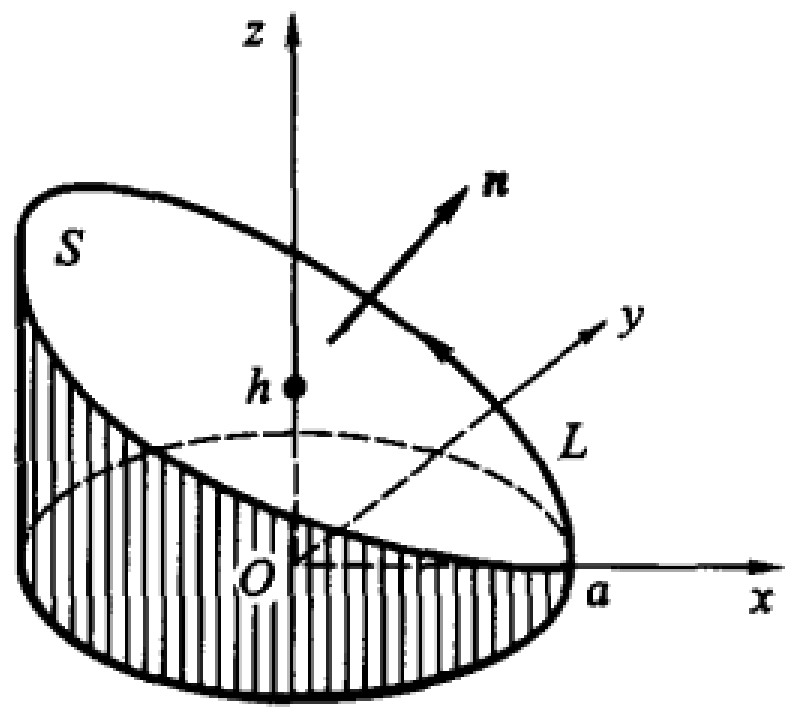
\includegraphics[width=0.28\textwidth]{work/figures/fig22-14}\caption{\relax}\label{fig:22-14}
\end{figure}

\begin{proof}[解法 1]
取平面 $\dfrac{x}{a}+\dfrac{z}{h}=1$ 上由交线围成的平面块为 $S$，并注意 $S$ 在 $Ozx$ 面上的投影为零，即 $\mathrm{d}z\mathrm{d}x=0$，由斯托克斯公式得
\[
\begin{aligned}
I&=\iint_{S}\begin{vmatrix}\mathrm{d}y\mathrm{d}z&\mathrm{d}z\mathrm{d}x&\mathrm{d}x\mathrm{d}y\\[3pt]\dfrac{\partial}{\partial x}&\dfrac{\partial}{\partial y}&\dfrac{\partial}{\partial z}\\[3pt] y-z&z-x&x-y\end{vmatrix}\\
&=2\iint_{S}\mathrm{d}y\mathrm{d}z+\mathrm{d}x\mathrm{d}y=-2\iint_{D_{yz}}\mathrm{d}y\mathrm{d}z-2\iint_{D_{xy}}\mathrm{d}x\mathrm{d}y\\
&=-2(\pi ah+\pi a^{2})=-2\pi a(h+a).
\end{aligned}
\]
最后一个等式是因为 $D_{yz}$ 是半轴分别为 $a$ 与 $h$ 的椭圆，其面积为 $\pi ah$，而 $D_{xy}$ 是圆 $x^{2}+y^{2}\leqslant a^{2}$，其面积为 $\pi a^{2}$．
\end{proof}

\begin{proof}[解法 2]
取曲面 $S$ 同解法 1，则 $S$ 的单位法向量
\[
\bm{n}=\left(\frac{h}{\sqrt{a^{2}+h^{2}}},0,\frac{a}{\sqrt{a^{2}+h^{2}}}\right)=(\cos\alpha,\cos\beta,\cos\gamma)
\]
是常向量，$S$ 是半轴分别为 $a$ 和 $\sqrt{a^{2}+h^{2}}$ 的椭圆．因此
\[
\begin{aligned}
I&=\iint_{S}\begin{vmatrix}\cos\alpha&\cos\beta&\cos\gamma\\[3pt]\dfrac{\partial}{\partial x}&\dfrac{\partial}{\partial y}&\dfrac{\partial}{\partial z}\\[3pt] y-z&z-x&x-y\end{vmatrix}\mathrm{d}S\\
&=-2\iint_{S}(\cos\alpha+\cos\gamma)\mathrm{d}S=-2\frac{a+h}{\sqrt{a^{2}+h^{2}}}\iint_{S}\mathrm{d}S\\
&=-2\frac{a+h}{\sqrt{a^{2}+h^{2}}}\pi a\sqrt{a^{2}+h^{2}}=-2\pi a(h+a).
\end{aligned}
\]
\end{proof}

\begin{proof}[解法 3]
也可以直接用线积分的计算公式．曲线 $L$ 的参数方程为
\[
x=a\cos t,\quad y=a\sin t,\quad z=h(1-\cos t),\ 0\leqslant t\leqslant 2\pi,
\]
则
\[
\begin{aligned}
I&=\int_{0}^{2\pi}\left\{\left[a\sin t-h(1-\cos t)\right](-a\sin t)\right.\\
&\quad\left.+\left[h(1-\cos t)-a\cos t\right]a\cos t+a(\cos t-\sin t)h\sin t\right\}\mathrm{d}t\\
&=\int_{0}^{2\pi}\left(-a^{2}-ah+ah\sin t+ah\cos t\right)\mathrm{d}t\\
&=-2\pi a(a+h).
\end{aligned}
\]
\end{proof}

到此为止，我们对各种积分的概念及其相互间的关系已经有了较完整的认识．二重积分、三重积分、两种类型的曲线积分和两种类型的曲面积分，它们来自不同的物理背景，抽象出不同的数学定义，但却有着奇妙的联系．格林公式、高斯公式和斯托克斯公式描述了这些联系，反映出的共同点是它们都给出空间某形体的积分与其边界上的积分的关系．它们都是牛顿－莱布尼茨公式的推广．

\begin{xiti}
\item 应用格林公式计算下列积分：
\begin{ziti}
\item $\displaystyle\oint_{L}xy^{2}\mathrm{d}y-x^{2}y\mathrm{d}x$，其中 $L$ 为椭圆 $\dfrac{x^{2}}{a^{2}}+\dfrac{y^{2}}{b^{2}}=1$，取正向；
\item $\displaystyle\oint_{L}(x+y)\mathrm{d}x+(x-y)\mathrm{d}y$，$L$ 同 (1)；
\item $\displaystyle\oint_{L}(x+y)^{2}\mathrm{d}x-(x^{2}+y^{2})\mathrm{d}y$，$L$ 是顶点为 $A(1,1)$，$B(3,2)$，$C(2,5)$ 的三角形的边界，取正向；
\item $\displaystyle\oint_{L}(x^{2}+y^{3})\mathrm{d}x-(x^{3}-y^{2})\mathrm{d}y$，$L$ 为 $x^{2}+y^{2}=1$，取正向；
\item $\displaystyle\oint_{L}\mathrm{e}^{y}\sin x\,\mathrm{d}x+\mathrm{e}^{-x}\sin y\,\mathrm{d}y$，$L$ 为矩形 $a\leqslant x\leqslant b$，$c\leqslant y\leqslant d$ 的边界，取正向；
\item $\displaystyle\oint_{L}\left[\left(y\sin xy+\cos(x+y)\right)\mathrm{d}x+\left(x\sin xy+\cos(x+y)\right)\mathrm{d}y\right]$，其中 $L$ 是任意逐段光滑闭曲线．
\end{ziti}
\item 利用格林公式计算下列曲线所围图形的面积：
\begin{ziti}
\item 双纽线 $r^{2}=a^{2}\cos 2\theta$；
\item 笛卡儿叶形线 $x^{3}+y^{3}=3axy$（$a>0$）；
\item $x=a(1+\cos^{2}t)\sin t$，$y=a\sin^{2}t\cos t$，$0\leqslant t\leqslant 2\pi$．
\end{ziti}
\item 利用高斯公式求下列积分：
\begin{ziti}
\item $\displaystyle\iint_{S}x^{2}\mathrm{d}y\mathrm{d}z+y^{2}\mathrm{d}z\mathrm{d}x+z^{2}\mathrm{d}x\mathrm{d}y$，其中（a）$S$ 为立方体 $0\leqslant x,y,z\leqslant a$ 的边界曲面外侧；（b）$S$ 为锥面 $x^{2}+y^{2}=z^{2}$（$0\leqslant z\leqslant h$），下侧．
\item $\displaystyle\iint_{S}x^{3}\mathrm{d}y\mathrm{d}z+y^{3}\mathrm{d}z\mathrm{d}x+z^{3}\mathrm{d}x\mathrm{d}y$，其中 $S$ 是单位球面的外侧；
\item 设 $S$ 是上半球面 $z=\sqrt{a^{2}-x^{2}-y^{2}}$ 的上侧，求（a）$\displaystyle\iint_{S}x\,\mathrm{d}y\mathrm{d}z+y\,\mathrm{d}z\mathrm{d}x+z\,\mathrm{d}x\mathrm{d}y$，（b）$\displaystyle\iint_{S}xz^{2}\mathrm{d}y\mathrm{d}z+(x^{2}y-z^{2})\mathrm{d}z\mathrm{d}x+(2xy+y^{2}z)\mathrm{d}x\mathrm{d}y$；
\item $\displaystyle\iint_{S}(x-y^{2}+z^{2})\mathrm{d}y\mathrm{d}z+(y-z^{2}+x^{2})\mathrm{d}z\mathrm{d}x+(z-x^{2}+y^{2})\mathrm{d}x\mathrm{d}y$，$S$ 是 $(x-a)^{2}+(y-b)^{2}+(z-c)^{2}=R^{2}$ 的外侧．
\end{ziti}
\item 用斯托克斯公式计算下列积分：
\begin{ziti}
\item $\displaystyle\oint_{L}x^{2}y^{3}\mathrm{d}x+\mathrm{d}y+z\mathrm{d}z$，其中（a）$L$ 为圆周 $x^{2}+y^{2}=a^{2}$，$z=0$，方向是逆时针；（b）$L$ 为 $y^{2}+z^{2}=1$，$x=y$ 所交的椭圆，从 $x$ 轴正向看去，按逆时针方向；
\item $\displaystyle\oint_{L}(y-z)\mathrm{d}x+(z-x)\mathrm{d}y+(x-y)\mathrm{d}z$，$L$ 是从 $(a,0,0)$ 经 $(0,a,0)$ 至 $(0,0,a)$ 回到 $(a,0,0)$ 的三角形；
\item $\displaystyle\oint_{L}(y^{2}+z^{2})\mathrm{d}x+(x^{2}+z^{2})\mathrm{d}y+(x^{2}+y^{2})\mathrm{d}z$，其中（a）$L$ 为 $x+y+z=1$ 与三坐标平面的交线，其方向与所围平面区域上侧构成右手法则，（b）$L$ 是曲线 $x^{2}+y^{2}+z^{2}=2Rx$，$x^{2}+y^{2}=2rx$（$0<r<R$，$z>0$），它的方向与所围曲面的上侧构成右手法则；
\item $\displaystyle\oint_{L}y\,\mathrm{d}x+z\,\mathrm{d}y+x\,\mathrm{d}z$，$L$ 是 $x^{2}+y^{2}+z^{2}=a^{2}$，$x+y+z=0$，从 $x$ 轴正向看去圆周是逆时针方向．
\end{ziti}
\item 设 $L$ 为平面上封闭曲线，$l$ 为平面上任意方向，证明
\[
\oint_{L}\cos(\bm{n},l)\mathrm{d}s=0,
\]
其中 $\bm{n}$ 是 $L$ 的外法线方向．
\item 设 $S$ 是封闭曲面，$l$ 为任意固定方向，证明
\[
\oiint_{S}\cos(\bm{n},l)\mathrm{d}S=0.
\]
\item 求 $I=\displaystyle\oint_{L}\left[x\cos(\bm{n},x)+y\cos(\bm{n},y)\right]\mathrm{d}s$，$L$ 为包围有界区域 $D$ 的光滑闭曲线，$\bm{n}$ 为 $L$ 的外法向．
\item 证明高斯积分
\[
\oint_{L}\frac{\cos(\bm{r},\bm{n})}{r}\mathrm{d}s=0,
\]
其中 $L$ 是平面上一单连通区域 $\sigma$ 的边界，而 $r$ 是 $L$ 上一点到 $\sigma$ 外某一定点的距离，$\bm{n}$ 是 $L$ 的外法线方向．又若 $r$ 表示 $L$ 上一点到 $\sigma$ 内某一定点的距离，则这个积分之值等于 $2\pi$．
\item 计算高斯积分
\[
\iint_{S}\frac{\cos(\bm{r},\bm{n})}{r^{2}}\mathrm{d}S,
\]
其中 $S$ 为简单封闭光滑曲面，$\bm{n}$ 为曲面 $S$ 上在点 $(\xi,\eta,\zeta)$ 处的外法向，$\bm{r}=(\xi-x)\bm{i}+(\eta-y)\bm{j}+(\zeta-z)\bm{k}$，$r=|\bm{r}|$．试对下列两种情形进行讨论：（1）曲面 $S$ 包围的区域不含 $(x,y,z)$ 点；（2）曲面 $S$ 包围的区域含 $(x,y,z)$ 点．
\item 求证：
\[
\iiint_{V}\frac{\mathrm{d}x\mathrm{d}y\mathrm{d}z}{r}=\frac{1}{2}\oiint_{S}\cos(\bm{r},\bm{n})\mathrm{d}S,
\]
其中 $S$ 是包围 $V$ 的分片光滑封闭曲面，$\bm{n}$ 为 $S$ 的外法线方向，$\bm{r}=(x,y,z)$，$r=|\bm{r}|$．分下列两种情形进行讨论：（1）$V$ 中不含原点 $(0,0,0)$；（2）$V$ 中含原点 $(0,0,0)$ 时，令
\[
\iiint_{V}\frac{\mathrm{d}x\mathrm{d}y\mathrm{d}z}{r}=\lim_{\varepsilon\to 0^{+}}\iiint_{V-V_{\varepsilon}}\frac{\mathrm{d}x\mathrm{d}y\mathrm{d}z}{r},
\]
其中 $V_{\varepsilon}$ 是以原点为心，以 $\varepsilon$ 为半径的球．
\item 利用高斯公式变换以下积分：
\begin{ziti}
\item $\displaystyle\iint_{S}xy\,\mathrm{d}x\mathrm{d}y+xz\,\mathrm{d}z\mathrm{d}x+yz\,\mathrm{d}y\mathrm{d}z$；
\item $\displaystyle\iint_{S}\left(\frac{\partial u}{\partial x}\cos\alpha+\frac{\partial u}{\partial y}\cos\beta+\frac{\partial u}{\partial z}\cos\gamma\right)\mathrm{d}S$，其中 $\cos\alpha,\cos\beta,\cos\gamma$ 是曲面的外法线方向余弦．
\end{ziti}
\item 设 $u(x,y)$，$v(x,y)$ 是具有二阶连续偏导数的函数，并设
\[
\Delta u=\frac{\partial^{2}u}{\partial x^{2}}+\frac{\partial^{2}u}{\partial y^{2}}.
\]
证明：
\begin{ziti}
\item $\displaystyle\iint_{\sigma}\Delta u\,\mathrm{d}x\mathrm{d}y=\oint_{l}\frac{\partial u}{\partial n}\,\mathrm{d}s$；
\item $\displaystyle\iint_{\sigma}v\Delta u\,\mathrm{d}x\mathrm{d}y=-\iint_{\sigma}\left(\frac{\partial u}{\partial x}\frac{\partial v}{\partial x}+\frac{\partial u}{\partial y}\frac{\partial v}{\partial y}\right)\mathrm{d}x\mathrm{d}y+\oint_{l}v\frac{\partial u}{\partial n}\mathrm{d}s$；
\item $\displaystyle\iint_{\sigma}\left(u\Delta v-v\Delta u\right)\mathrm{d}x\mathrm{d}y=-\oint_{l}\left(v\frac{\partial u}{\partial n}-u\frac{\partial v}{\partial n}\right)\mathrm{d}s$.
\end{ziti}
其中 $\sigma$ 为闭曲线 $l$ 所围的平面区域，$\dfrac{\partial u}{\partial n}$，$\dfrac{\partial v}{\partial n}$ 为沿 $l$ 外法线的方向导数．
\item 设 $\Delta u=\dfrac{\partial^{2}u}{\partial x^{2}}+\dfrac{\partial^{2}u}{\partial y^{2}}+\dfrac{\partial^{2}u}{\partial z^{2}}$，$S$ 是 $V$ 的边界曲面，证明：
\begin{ziti}
\item $\displaystyle\iiint_{V}\Delta u\,\mathrm{d}x\mathrm{d}y\mathrm{d}z=\iint_{S}\frac{\partial u}{\partial n}\,\mathrm{d}S$；
\item $\displaystyle\iint_{S}u\frac{\partial u}{\partial n}\mathrm{d}S=\iiint_{V}\left[\left(\frac{\partial u}{\partial x}\right)^{2}+\left(\frac{\partial u}{\partial y}\right)^{2}+\left(\frac{\partial u}{\partial z}\right)^{2}\right]\mathrm{d}x\mathrm{d}y\mathrm{d}z+\iiint_{V}u\Delta u\,\mathrm{d}x\mathrm{d}y\mathrm{d}z$.
\end{ziti}
式中 $u$ 在 $V$ 及其边界曲面 $S$ 上有连续的二阶偏导数，$\dfrac{\partial u}{\partial n}$ 为沿曲面 $S$ 的外法线的方向导数．
\item 计算下列曲面积分：
\begin{ziti}
\item $\displaystyle\iint_{S}(x^{2}-y^{2})\mathrm{d}y\mathrm{d}z+(y^{2}-z^{2})\mathrm{d}z\mathrm{d}x+2z(y-x)\mathrm{d}x\mathrm{d}y$，其中 $S$ 是 $\dfrac{x^{2}}{a^{2}}+\dfrac{y^{2}}{b^{2}}+\dfrac{z^{2}}{c^{2}}=1$（$z\geqslant 0$）下侧；
\item $\displaystyle\iint_{S}(x+\cos y)\,\mathrm{d}y\mathrm{d}z+(y+\cos z)\,\mathrm{d}z\mathrm{d}x+(z+\cos x)\,\mathrm{d}x\mathrm{d}y$，$S$ 是立体 $\Omega$ 的边界面，而立体 $\Omega$ 由 $x+y+z=1$ 和三坐标面围成；
\item $\displaystyle\iint_{S}\bm{F}\cdot\bm{n}\,\mathrm{d}S$，其中 $\bm{F}=x^{3}\bm{i}+y^{3}\bm{j}+z^{3}\bm{k}$，$\bm{n}$ 是 $S$ 的外法向，$S$ 为 $x^{2}+y^{2}+z^{2}=a^{2}(z\geqslant 0)$ 上侧；
\item $\displaystyle\iint_{S}\left(\frac{x^{3}}{a^{2}}+yz\right)\mathrm{d}y\mathrm{d}z+\left(\frac{y^{3}}{b^{2}}+z^{3}x^{2}\right)\mathrm{d}z\mathrm{d}x+\left(\frac{z^{3}}{c^{2}}+x^{3}y^{3}\right)\mathrm{d}x\mathrm{d}y$，$S$ 是 $\dfrac{x^{2}}{a^{2}}+\dfrac{y^{2}}{b^{2}}+\dfrac{z^{2}}{c^{2}}=1$（$x\geqslant 0$）后侧．
\end{ziti}
\item 证明由曲面 $S$ 所包围的体积等于
\[
V=\frac{1}{3}\iint_{S}\left(x\cos\alpha+y\cos\beta+z\cos\gamma\right)\mathrm{d}S,
\]
式中 $\cos\alpha$，$\cos\beta$，$\cos\gamma$ 为曲面 $S$ 的外法线的方向余弦．
\item 若 $L$ 是平面 $x\cos\alpha+y\cos\beta+z\cos\gamma-p=0$ 上逐段光滑的闭曲线，它所包围区域的面积为 $S$，求
\[
\oint_{L}\begin{vmatrix}\mathrm{d}x&\mathrm{d}y&\mathrm{d}z\\ \cos\alpha&\cos\beta&\cos\gamma\\ x&y&z\end{vmatrix},
\]
其中 $L$ 依正向进行．
\item 设 $P$，$Q$，$R$ 有连续偏导数，且对任意光滑闭曲面 $S$，有
\[
\iint_{S}P\mathrm{d}y\mathrm{d}z+Q\mathrm{d}z\mathrm{d}x+R\mathrm{d}x\mathrm{d}y=0.
\]
证明 $\dfrac{\partial P}{\partial x}+\dfrac{\partial Q}{\partial y}+\dfrac{\partial R}{\partial z}=0$．
\item 设 $P(x,y)$，$Q(x,y)$ 在全平面上有连续偏导数，而且以任意点 $(x_{0},y_{0})$ 为中心，以任意正数 $r$ 为半径的上半圆 $l$：$x=x_{0}+r\cos\theta$，$y=y_{0}+r\sin\theta$（$0\leqslant\theta\leqslant\pi$），恒有
\[
\int_{l}P(x,y)\mathrm{d}x+Q(x,y)\mathrm{d}y=0,
\]
求证：$P(x,y)=0$，$\dfrac{\partial Q}{\partial x}=0$．
\end{xiti}

\section{积分与路径无关}

考虑积分
\[
\int_{L}\frac{x\mathrm{d}y-y\mathrm{d}x}{x^{2}+y^{2}}.
\]
对于圆 $x=a\cos\theta$，$y=a\sin\theta$，记 $L_{1}$ 为上半圆周，$L_{2}$ 为下半圆周，方向都是从 $(-a,0)$ 点到 $(a,0)$ 点．则
\[
\begin{aligned}
\int_{L_{1}}\frac{x\mathrm{d}y-y\mathrm{d}x}{x^{2}+y^{2}}&=-\pi,\\
\int_{L_{2}}\frac{x\mathrm{d}y-y\mathrm{d}x}{x^{2}+y^{2}}&=\pi.
\end{aligned}
\]
它表明尽管 $L_{1}$ 与 $L_{2}$ 有相同的起点和相同的终点，但由于路径不同，积分值也不同，即积分与路径有关．又若 $L$ 是起点为 $(-a,0)$，终点为 $(a,0)$ 的光滑曲线，且与 $L_{1}$ 构成不包围原点的闭曲线，由格林公式有
\[
\left(\int_{L_{1}}-\int_{L}\right)\frac{x\mathrm{d}y-y\mathrm{d}x}{x^{2}+y^{2}}=0,
\]
即 $\displaystyle\int_{L}\frac{x\mathrm{d}y-y\mathrm{d}x}{x^{2}+y^{2}}=\int_{L_{1}}\frac{x\mathrm{d}y-y\mathrm{d}x}{x^{2}+y^{2}}=-\pi$．
\begin{figure}[htbp]
\centering
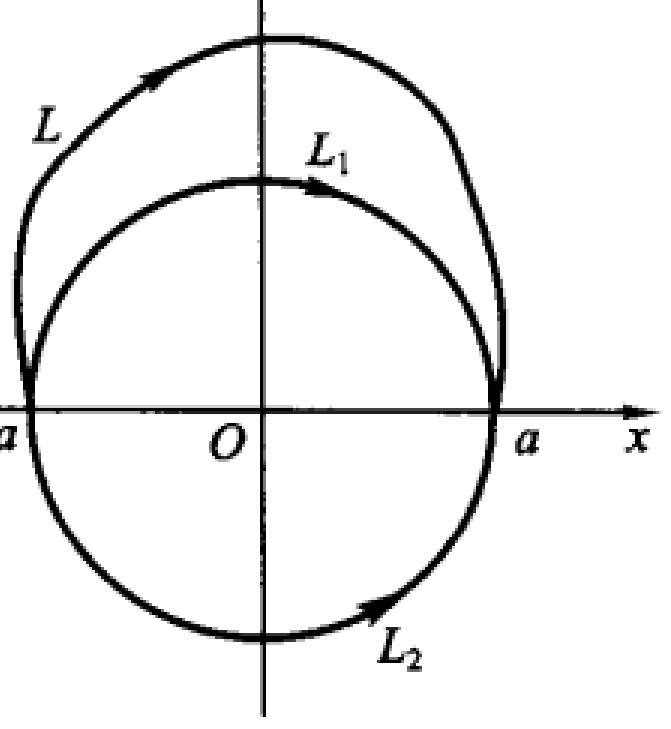
\includegraphics[width=0.28\textwidth]{work/figures/fig22-15}\caption{\relax}\label{fig:22-15}
\end{figure}
它又表明从 $(-a,0)$ 出发经上半平面越过 $y$ 轴到 $(a,0)$ 点的任一条光滑曲线的积分与路径无关，积分值都是 $-\pi$．

在什么条件下积分与路径无关呢？

\begin{theorem}\label{thm:22-4}
设 $D$ 是平面单连通区域，函数 $P(x,y)$，$Q(x,y)$ 在 $D$ 上有连续偏导数，则下列四断言等价：
\begin{enumerate}[label=（\arabic*）]
\item 沿 $D$ 中任一逐段光滑的闭曲线 $L$，有 $\displaystyle\oint_{L}P\mathrm{d}x+Q\mathrm{d}y=0$；
\item 对 $D$ 中任一逐段光滑曲线 $L$，曲线积分 $\displaystyle\int_{L}P\mathrm{d}x+Q\mathrm{d}y$ 与路径无关，只与 $L$ 的起点与终点有关；
\item 微分式 $P\mathrm{d}x+Q\mathrm{d}y$ 在 $D$ 内是某函数 $u(x,y)$ 的全微分，即有 $\mathrm{d}u=P\mathrm{d}x+Q\mathrm{d}y$；
\item 在 $D$ 内每一点有 $\dfrac{\partial P}{\partial y}=\dfrac{\partial Q}{\partial x}$．
\end{enumerate}
\end{theorem}

\begin{proof}
（1）$\Rightarrow$（2）．设 $A$、$B$ 是 $D$ 内任意两点，$L_{1}$ 和 $L_{2}$ 是完全含于 $D$ 内的任意两条连结 $A$、$B$ 的逐段光滑曲线，方向都是从 $A$ 到 $B$．于是 $L_{1}$ 与 $L_{2}$ 的反向构成完全含于 $D$ 内的一条闭曲线，由（1）知
\[
\left(\int_{L_{1}}-\int_{L_{2}}\right)P\mathrm{d}x+Q\mathrm{d}y=0,
\]
即
\[
\int_{L_{1}}P\mathrm{d}x+Q\mathrm{d}y=\int_{L_{2}}P\mathrm{d}x+Q\mathrm{d}y,
\]
这表明（2）成立．

（2）$\Rightarrow$（3）．设 $A(x_{0},y_{0})$，$B(x,y)$ 为 $D$ 内的两点，由（2）知，从 $A$ 到 $B$ 的积分只与起点和终点有关，而与路径无关，把起点固定在 $A(x_{0},y_{0})$，则积分便是终点 $(x,y)$ 的函数，记为
\begin{figure}[htbp]
\centering
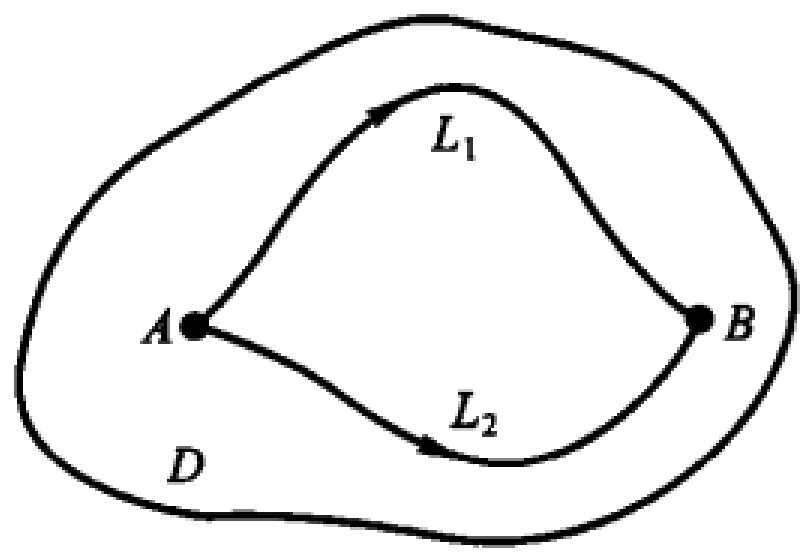
\includegraphics[width=0.28\textwidth]{work/figures/fig22-16}\caption{\relax}\label{fig:22-16}
\end{figure}
\[
u(x,y)=\int_{(x_{0},y_{0})}^{(x,y)}P\mathrm{d}x+Q\mathrm{d}y.
\]
显然 $u(x,y)$ 定义在 $D$ 内，下面要证
\[
\frac{\partial u}{\partial x}=P(x,y),\qquad\frac{\partial u}{\partial y}=Q(x,y).
\]
由于 $B(x,y)$ 是 $D$ 的内点，当 $|\Delta x|$ 充分小时，$(x+\Delta x,y)\in D$．考虑
\[
\begin{aligned}
&u(x+\Delta x,y)-u(x,y)\\
=&\int_{(x_{0},y_{0})}^{(x+\Delta x,y)}P\mathrm{d}x+Q\mathrm{d}y-\int_{(x_{0},y_{0})}^{(x,y)}P\mathrm{d}x+Q\mathrm{d}y.
\end{aligned}
\]
由于积分与路径无关，取从 $(x_{0},y_{0})$ 到 $(x+\Delta x,y)$ 的路径经过 $B(x,y)$ 点，而从 $B(x,y)$ 到 $(x+\Delta x,y)$ 的路径则取连结两点的直线段，再用积分中值定理，有
\begin{figure}[htbp]
\centering
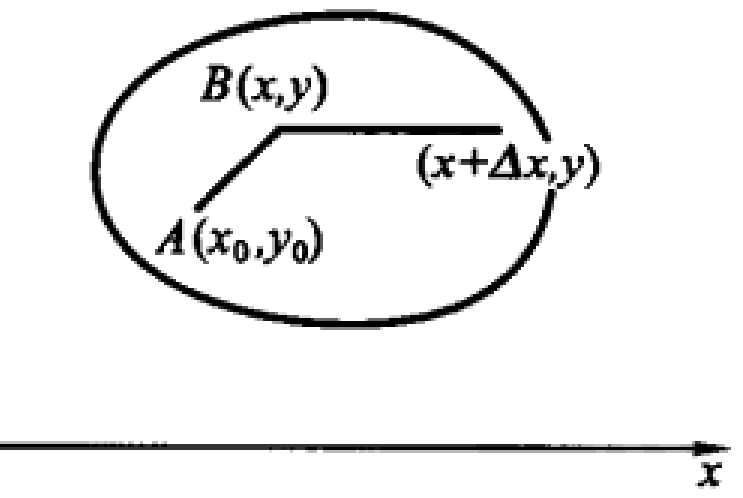
\includegraphics[width=0.28\textwidth]{work/figures/fig22-17}\caption{\relax}\label{fig:22-17}
\end{figure}
\[
\begin{aligned}
&u(x+\Delta x,y)-u(x,y)\\
=&\int_{(x,y)}^{(x+\Delta x,y)}P\mathrm{d}x+Q\mathrm{d}y=\int_{(x,y)}^{(x+\Delta x,y)}P(x,y)\mathrm{d}x\\
=&\int_{x}^{x+\Delta x}P(x,y)\mathrm{d}x=P(\xi,y)\Delta x,
\end{aligned}
\]
其中 $\xi$ 在 $x$ 与 $x+\Delta x$ 之间．因为 $P(x,y)$ 在 $D$ 内连续，所以
\[
\begin{aligned}
\frac{\partial u}{\partial x}&=\lim_{\Delta x\to 0}\frac{u(x+\Delta x,y)-u(x,y)}{\Delta x}\\
&=\lim_{\Delta x\to 0}P(\xi,y)=P(x,y).
\end{aligned}
\]
同理可证 $\dfrac{\partial u}{\partial y}=Q(x,y)$．由 $\dfrac{\partial u}{\partial x}=P(x,y)$ 和 $\dfrac{\partial u}{\partial y}=Q(x,y)$ 都在 $D$ 内连续，知 $u(x,y)$ 在 $D$ 内可微，且有
\[
\mathrm{d}u=\frac{\partial u}{\partial x}\mathrm{d}x+\frac{\partial u}{\partial y}\mathrm{d}y=P(x,y)\mathrm{d}x+Q(x,y)\mathrm{d}y.
\]
（3）$\Rightarrow$（4）．已知 $\mathrm{d}u=P\mathrm{d}x+Q\mathrm{d}y$，因此
\[
\frac{\partial u}{\partial x}=P(x,y),\qquad\frac{\partial u}{\partial y}=Q(x,y),
\]
故
\[
\frac{\partial^{2}u}{\partial x\partial y}=\frac{\partial P}{\partial y},\quad\frac{\partial^{2}u}{\partial y\partial x}=\frac{\partial Q}{\partial x}.
\]
根据 $P$，$Q$ 在 $D$ 内有连续的偏导数，有 $\dfrac{\partial^{2}u}{\partial x\partial y}=\dfrac{\partial^{2}u}{\partial y\partial x}$，即
\[
\frac{\partial P}{\partial y}=\frac{\partial Q}{\partial x}.
\]
（4）$\Rightarrow$（1）．设 $L$ 是完全含于 $D$ 内的任一逐段光滑的闭曲线，$L$ 所围区域为 $\sigma$，$L$ 的方向关于 $\sigma$ 为正向．因为 $D$ 是单连通区域，所以 $\sigma$ 完全含于 $D$ 内，因此在 $\sigma$ 上 $\dfrac{\partial Q}{\partial x}=\dfrac{\partial P}{\partial y}$．故由格林公式，得
\[
\oint_{L}P\mathrm{d}x+Q\mathrm{d}y=\iint_{\sigma}\left(\frac{\partial Q}{\partial x}-\frac{\partial P}{\partial y}\right)\mathrm{d}x\mathrm{d}y=0.
\]
定理~\ref{thm:22-4} 证完．
\end{proof}

回头看看定理的证明，不难发现，``$D$ 是单连通区域''的条件只在（4）$\Rightarrow$（1）的证明中用到．可以证明，若 $D$ 是复连通区域，则（1）、（2）、（3）仍是等价的（证明留给读者）．但对（1）或（2）或（3）来说，断言（4）只是必要的，而不是充分的，即当（4）成立时，未必有（1）、（2）、（3）成立．在这里，单连通区域的条件是重要的．例如本节开头的例子
\[
\int_{L}\frac{x\mathrm{d}y-y\mathrm{d}x}{x^{2}+y^{2}}=\int_{L}P\mathrm{d}x+Q\mathrm{d}y.
\]
我们已经计算过，从 $(-a,0)$ 出发沿上半圆周 $L_{1}$ 到 $(a,0)$ 点的积分不等于沿下半圆周 $L_{2}$ 到 $(a,0)$ 点的积分．其原因就在于 $L_{1}$ 和 $L_{2}$ 所围的区域包含了坐标原点，而 $\dfrac{\partial Q}{\partial x}=\dfrac{\partial P}{\partial y}$ 在原点 $(0,0)$ 不成立．换句话说，既包含 $L_{1}$ 和 $L_{2}$，又能使 $\dfrac{\partial Q}{\partial x}=\dfrac{\partial P}{\partial y}$ 处处成立的区域只能是复连通区域．这个例子表明，在复连通区域 $D$ 上，尽管条件（4）成立，也不能保证沿 $D$ 内的光滑曲线的积分与路径无关．

使 $\dfrac{\partial Q}{\partial x}=\dfrac{\partial P}{\partial y}$ 不成立的点称为积分 $\displaystyle\int_{L}P\mathrm{d}x+Q\mathrm{d}y$ 的\emph{奇点}．在单连通区域中把这些``奇点''挖去，则单连通性受到破坏而成为复连通区域 $D$，但在复连通区域 $D$ 中条件 $\dfrac{\partial Q}{\partial x}=\dfrac{\partial P}{\partial y}$ 却处处得到满足．这时有下述结论：

（1）对 $D$ 内任意一条不包围奇点的闭曲线 $L$，有
\[
\oint_{L}P\mathrm{d}x+Q\mathrm{d}y=0.
\]
（2）环绕某一奇点的任意两条简单闭曲线 $L_{1}$ 和 $L_{2}$ 的正向的积分相等，即
\[
\oint_{L_{1}}P\mathrm{d}x+Q\mathrm{d}y=\oint_{L_{2}}P\mathrm{d}x+Q\mathrm{d}y.
\]
这个公共值称为该奇点的\emph{循环常数}．
\begin{figure}[htbp]
\centering
\begin{minipage}[c]{0.44\textwidth}\centering
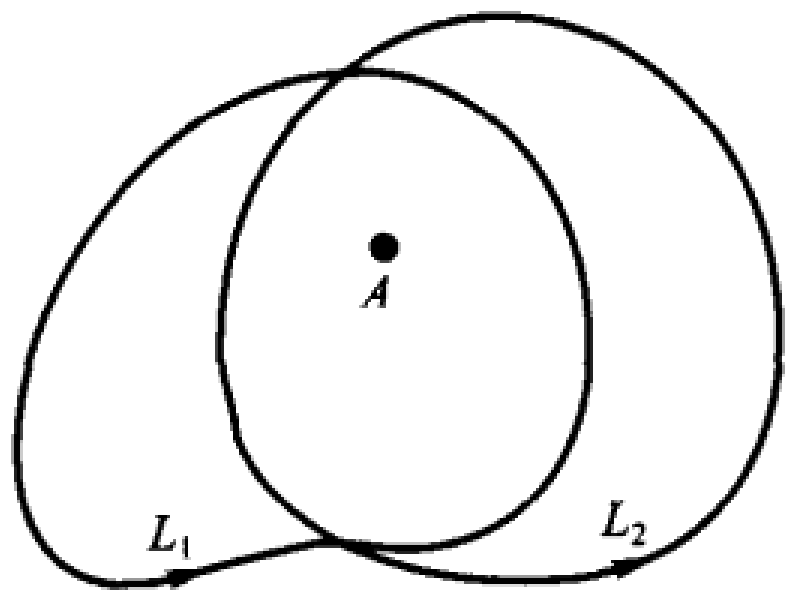
\includegraphics[width=\textwidth]{work/figures/fig22-18}\caption{\relax}\label{fig:22-18}
\end{minipage}\hfill
\begin{minipage}[c]{0.30\textwidth}\centering
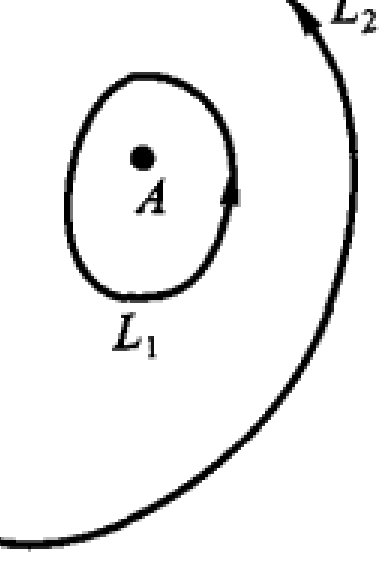
\includegraphics[width=\textwidth]{work/figures/fig22-19}\caption{\relax}\label{fig:22-19}
\end{minipage}
\end{figure}

事实上，若 $L$ 是 $D$ 内任意一条不包围奇点的闭曲线，则在 $L$ 包围的区域 $\sigma$ 内处处成立 $\dfrac{\partial Q}{\partial x}=\dfrac{\partial P}{\partial y}$，由格林公式即证得（1）成立．若 $L_{1}$ 和 $L_{2}$ 是两条包围奇点的简单闭曲线，且方向相同，记 $L_{1}$ 的反方向为 $L_{1}^{-}$，$\sigma$ 是 $L_{1}^{-}$ 和 $L_{2}$ 所围的不含奇点的平面区域（图~\ref{fig:22-18} 和图~\ref{fig:22-19}），则由格林公式知
\[
\left(\int_{L_{1}^{-}}+\int_{L_{2}}\right)P\mathrm{d}x+Q\mathrm{d}y=\iint_{\sigma}\left(\frac{\partial Q}{\partial x}-\frac{\partial P}{\partial y}\right)\mathrm{d}x\mathrm{d}y=0,
\]
即
\[
\int_{L_{1}}P\mathrm{d}x+Q\mathrm{d}y=\int_{L_{2}}P\mathrm{d}x+Q\mathrm{d}y.
\]
从前面的例子可知，积分 $I=\displaystyle\oint_{L}\frac{x\mathrm{d}y-y\mathrm{d}x}{x^{2}+y^{2}}$ 只有一个奇点 $(0,0)$，它的循环常数是 $2\pi$．因此，若 $L$ 是不包围 $(0,0)$ 点的闭曲线，则 $I=0$；若 $L$ 是包围 $(0,0)$ 点的简单闭曲线的正向，则 $I=2\pi$．

进一步还有下述结论：

（3）环绕某一奇点 $n$ 圈的光滑闭曲线 $L$，其中 $n_{1}$ 圈是正向，$n_{2}$ 圈是负向，$n_{1}+n_{2}=n$，则积分 $I=\displaystyle\oint_{L}P\mathrm{d}x+Q\mathrm{d}y$ 等于该点循环常数的 $n_{1}-n_{2}$ 倍．图~\ref{fig:22-20} 是绕 $A$ 两圈的例子．
\begin{figure}[htbp]
\centering
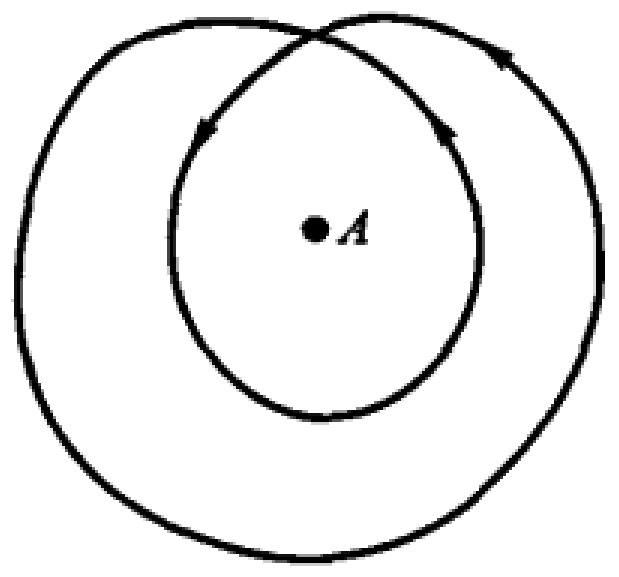
\includegraphics[width=0.22\textwidth]{work/figures/fig22-20}\caption{\relax}\label{fig:22-20}
\end{figure}

（4）若不自相交光滑闭曲线 $L$ 包围了 $k$ 个奇点，则沿 $L$ 正向的积分 $I=\displaystyle\oint_{L}P\mathrm{d}x+Q\mathrm{d}y$ 等于这 $k$ 个奇点的循环常数之和．

\begin{example}\label{ex:22-2-1}
求 $I=\displaystyle\oint_{L}\frac{x\,\mathrm{d}x+y\,\mathrm{d}y}{\sqrt{x^{2}+y^{2}}}$，其中 $L$ 是任意一条不经过原点的闭曲线．
\end{example}

\begin{proof}[解]
记
\[
P(x,y)=\frac{x}{\sqrt{x^{2}+y^{2}}},\quad Q(x,y)=\frac{y}{\sqrt{x^{2}+y^{2}}},
\]
则
\[
\frac{\partial Q}{\partial x}=\frac{\partial P}{\partial y}=-\frac{xy}{\left(x^{2}+y^{2}\right)^{3/2}},\quad(x,y)\neq(0,0).
\]
这说明积分只有一个奇点 $(0,0)$．为求其循环常数，取 $l$ 为单位圆 $x^{2}+y^{2}=1$ 的正向，则
\[
\oint_{l}\frac{x\mathrm{d}x+y\mathrm{d}y}{\sqrt{x^{2}+y^{2}}}=\oint_{l}x\mathrm{d}x+y\mathrm{d}y=\iint_{\sigma}0\,\mathrm{d}x\mathrm{d}y=0,
\]
其中 $\sigma$ 是 $x^{2}+y^{2}\leqslant 1$，即 $(0,0)$ 点的循环常数为 $0$，故对任意一条不经过原点的闭曲线 $L$，有 $I=0$．
\end{proof}

定理~\ref{thm:22-4} 的（2）、（3）表明，在积分与路径无关的条件下，存在函数 $u(x,y)$，使得 $u(x,y)$ 的全微分就是 $P\mathrm{d}x+Q\mathrm{d}y$，即
\[
\mathrm{d}u(x,y)=P(x,y)\mathrm{d}x+Q(x,y)\mathrm{d}y.
\]
这时我们称函数 $u(x,y)$ 为 $P\mathrm{d}x+Q\mathrm{d}y$ 的\emph{原函数}．在这种情况下，对 $D$ 内任意两点 $A$ 与 $B$，有
\[
\int_{A}^{B}P\mathrm{d}x+Q\mathrm{d}y=\int_{A}^{B}\mathrm{d}u=u(x,y)\bigg|_{A}^{B}=u(B)-u(A).
\]
问题是原函数 $u(x,y)$ 如何求呢？

从定理的证明知道 $P\mathrm{d}x+Q\mathrm{d}y$ 的一个原函数可表为
\[
u(x,y)=\int_{(x_{0},y_{0})}^{(x,y)}P(x,y)\mathrm{d}x+Q(x,y)\mathrm{d}y.
\]
由于积分与路径无关，可以任意地选择一条起点为 $(x_{0},y_{0})$，终点为 $(x,y)$ 且完全含于 $D$ 内的路径．为计算方便，通常是取含于 $D$ 内如图~\ref{fig:22-21} 所示的折线段，这时有
\begin{figure}[htbp]
\centering
\begin{minipage}[c]{0.42\textwidth}\centering
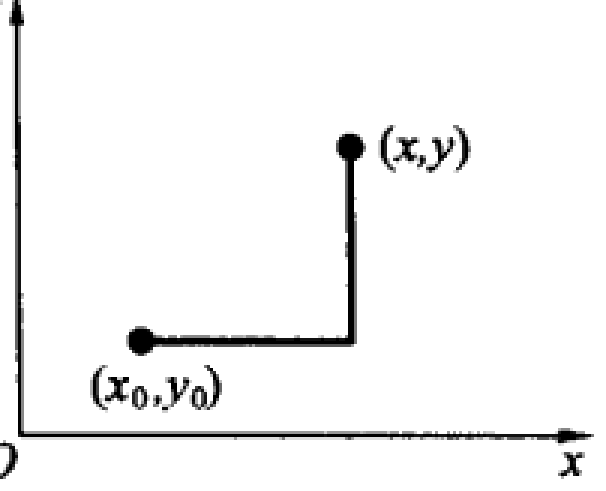
\includegraphics[width=\textwidth]{work/figures/fig22-21a}
\end{minipage}\hfill
\begin{minipage}[c]{0.42\textwidth}\centering
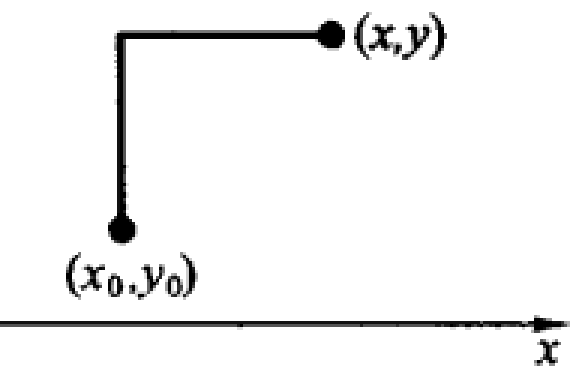
\includegraphics[width=\textwidth]{work/figures/fig22-21b}
\end{minipage}\caption{\relax}\label{fig:22-21}
\end{figure}
\[
u(x,y)=\int_{y_{0}}^{y}Q(x_{0},y)\mathrm{d}y+\int_{x_{0}}^{x}P(x,y)\mathrm{d}x+C,
\]
或
\[
u(x,y)=\int_{x_{0}}^{x}P(x,y_{0})\mathrm{d}x+\int_{y_{0}}^{y}Q(x,y)\mathrm{d}y+C.
\]
其中 $C$ 为常数．这是两个定积分之和，一般说来，我们是会计算的．

\begin{example}\label{ex:22-2-2}
求 $\left(\cos x+2x\sin y\right)\mathrm{d}x+\left(x^{2}\cos y\right)\mathrm{d}y$ 的原函数．
\end{example}

\begin{proof}[解]
设 $P(x,y)=\cos x+2x\sin y$，$Q(x,y)=x^{2}\cos y$．易见 $P$、$Q$ 在全平面上有连续的偏导数，且
\[
\frac{\partial P}{\partial y}=2x\cos y=\frac{\partial Q}{\partial x}.
\]
因此在平面上的任意光滑曲线 $AB$ 的积分
\[
\int_{\widehat{AB}}\left(\cos x+2x\sin y\right)\mathrm{d}x+\left(x^{2}\cos y\right)\mathrm{d}y
\]
只与起点 $A$ 和终点 $B$ 有关，而与路径的选择无关．取 $A=(0,0)$，$B=(x,y)$，则有
\[
\begin{aligned}
u(x,y)&=\int_{0}^{x}P(x,0)\mathrm{d}x+\int_{0}^{y}Q(x,y)\mathrm{d}y+C\\
&=\int_{0}^{x}\cos x\,\mathrm{d}x+\int_{0}^{y}x^{2}\cos y\,\mathrm{d}y+C\\
&=\sin x+x^{2}\sin y+C,
\end{aligned}
\]
这便是所要求的原函数．

当然，在简单的情形下我们可以通过观察直接凑微分，例如
\[
\begin{aligned}
&\left(\cos x+2x\sin y\right)\mathrm{d}x+\left(x^{2}\cos y\right)\mathrm{d}y\\
=&\cos x\,\mathrm{d}x+\left(2x\sin y\,\mathrm{d}x+x^{2}\cos y\,\mathrm{d}y\right)\\
=&\mathrm{d}\sin x+\mathrm{d}\left(x^{2}\sin y\right)\\
=&\mathrm{d}\left(\sin x+x^{2}\sin y\right),
\end{aligned}
\]
故 $u(x,y)=\sin x+x^{2}\sin y+C$．这样也得到同样的结果．
\end{proof}

定理~\ref{thm:22-4} 可以推广到三维的情形．

\begin{theorem}\label{thm:22-5}
设 $V$ 是空间的单连通区域，函数 $P$、$Q$、$R$ 在 $V$ 上有连续偏导数，则下列四断言等价：
\begin{enumerate}[label=（\arabic*）]
\item 沿 $V$ 内任一逐段光滑闭曲线 $L$，有 $\displaystyle\oint_{L}P\mathrm{d}x+Q\mathrm{d}y+R\mathrm{d}z=0$；
\item 对 $V$ 内任一逐段光滑曲线 $L$，曲线积分 $\displaystyle\int_{L}P\mathrm{d}x+Q\mathrm{d}y+R\mathrm{d}z$ 与路径无关，只与 $L$ 的起点与终点有关；
\item 微分式 $P\mathrm{d}x+Q\mathrm{d}y+R\mathrm{d}z$ 在 $V$ 内是某函数 $u(x,y,z)$ 的全微分，即 $\mathrm{d}u=P\mathrm{d}x+Q\mathrm{d}y+R\mathrm{d}z$；
\item 在 $V$ 内每一点有 $\dfrac{\partial P}{\partial y}=\dfrac{\partial Q}{\partial x}$，$\dfrac{\partial Q}{\partial z}=\dfrac{\partial R}{\partial y}$，$\dfrac{\partial R}{\partial x}=\dfrac{\partial P}{\partial z}$．
\end{enumerate}
\end{theorem}

定理~\ref{thm:22-5} 的证明可类似于定理~\ref{thm:22-4} 进行，困难在（4）$\Rightarrow$（1）时，如何用斯托克斯公式，我们不在此详述了．

断言（4）也可写为：在 $V$ 内每一点有
\[
\begin{vmatrix}\bm{i}&\bm{j}&\bm{k}\\[3pt]\dfrac{\partial}{\partial x}&\dfrac{\partial}{\partial y}&\dfrac{\partial}{\partial z}\\[3pt] P&Q&R\end{vmatrix}=\bm{0}.
\]

\begin{xiti}
\item 验证下列积分与路径无关，并求它们的值：
\begin{ziti}
\item $\displaystyle\int_{(0,0)}^{(1,1)}(x-y)(\mathrm{d}x-\mathrm{d}y)$；
\item $\displaystyle\int_{(2,1)}^{(1,2)}\frac{y\mathrm{d}x-x\mathrm{d}y}{x^{2}}$ 沿在右半平面的路径；
\item $\displaystyle\int_{(1,0)}^{(6,8)}\frac{x\mathrm{d}x+y\mathrm{d}y}{x^{2}+y^{2}}$ 沿不通过原点的路径；
\item $\displaystyle\int_{(0,0)}^{(a,b)}f(x+y)(\mathrm{d}x+\mathrm{d}y)$，式中 $f(u)$ 是连续函数；
\item $\displaystyle\int_{(2,1)}^{(1,2)}\varphi(x)\mathrm{d}x+\psi(y)\mathrm{d}y$，其中 $\varphi$，$\psi$ 为连续函数；
\item $\displaystyle\int_{(1,2,3)}^{(6,1,1)}yz\mathrm{d}x+xz\mathrm{d}y+xy\mathrm{d}z$；
\item $\displaystyle\int_{(1,1,1)}^{(2,3,-4)}x\,\mathrm{d}x+y^{2}\,\mathrm{d}y-z^{3}\,\mathrm{d}z$；
\item $\displaystyle\int_{(x_{1},y_{1},z_{1})}^{(x_{2},y_{2},z_{2})}\frac{x\mathrm{d}x+y\mathrm{d}y+z\mathrm{d}z}{\sqrt{x^{2}+y^{2}+z^{2}}}$，其中 $(x_{1},y_{1},z_{1})$，$(x_{2},y_{2},z_{2})$ 在球面 $x^{2}+y^{2}+z^{2}=a^{2}$ 上．
\end{ziti}
\item 求下列全微分的原函数：
\begin{ziti}
\item $\left(x^{2}+2xy-y^{2}\right)\mathrm{d}x+\left(x^{2}-2xy-y^{2}\right)\mathrm{d}y$；
\item $\left(2x\cos y-y^{2}\sin x\right)\mathrm{d}x+\left(2y\cos x-x^{2}\sin y\right)\mathrm{d}y$；
\item $\dfrac{a}{z}\mathrm{d}x+\dfrac{b}{z}\mathrm{d}y+\dfrac{-by-ax}{z^{2}}\mathrm{d}z$；
\item $\left(x^{2}-2yz\right)\mathrm{d}x+\left(y^{2}-2xz\right)\mathrm{d}y+\left(z^{2}-2xy\right)\mathrm{d}z$；
\item $\left(\mathrm{e}^{x}\sin y+2xy^{2}\right)\mathrm{d}x+\left(\mathrm{e}^{x}\cos y+2x^{2}y\right)\mathrm{d}y$；
\item $\left[\dfrac{x}{\left(x^{2}-y^{2}\right)^{2}}-\dfrac{1}{x}+2x^{2}\right]\mathrm{d}x+\left[\dfrac{1}{y}-\dfrac{y}{\left(x^{2}-y^{2}\right)^{2}}+3y^{3}\right]\mathrm{d}y+5z^{3}\mathrm{d}z$.
\end{ziti}
\item 函数 $F(x,y)$ 应满足什么条件才能使微分式
\[
F(x,y)(x\mathrm{d}x+y\mathrm{d}y)
\]
是全微分．
\item 验证
\[
P\mathrm{d}x+Q\mathrm{d}y=\frac{1}{2}\frac{x\mathrm{d}y-y\mathrm{d}x}{Ax^{2}+2Bxy+Cy^{2}}
\]
适合条件 $\dfrac{\partial P}{\partial y}=\dfrac{\partial Q}{\partial x}$，其中 $A$，$B$，$C$ 为常数，$AC-B^{2}>0$．求奇点 $(0,0)$ 的循环常数．
\item 求 $I=\displaystyle\oint_{L}\frac{x\,\mathrm{d}x+y\,\mathrm{d}y}{x^{2}+y^{2}}$，其中 $L$ 是不经过原点的简单闭曲线，取正向．设 $L$ 围成的区域为 $D$．（1）$D$ 不包含原点；（2）$D$ 包含原点在其内部．
\item 求
\[
I=\oint_{L}\left[\frac{y}{(x-2)^{2}+y^{2}}+\frac{y}{(x+2)^{2}+y^{2}}\right]\mathrm{d}x+\left[\frac{2-x}{(2-x)^{2}+y^{2}}+\frac{-(2+x)}{(2+x)^{2}+y^{2}}\right]\mathrm{d}y,
\]
其中 $L$ 是不经过 $(-2,0)$ 和 $(2,0)$ 点的简单闭曲线．
\item 设 $u(x,y)$ 在平面单连通区域 $D$ 上有二阶连续偏导数，证明 $u(x,y)$ 在 $D$ 内有 $\dfrac{\partial^{2}u}{\partial x^{2}}+\dfrac{\partial^{2}u}{\partial y^{2}}=0$ 的充要条件是对 $D$ 内任一简单光滑闭曲线 $L$，都有
\[
\oint_{L}\frac{\partial u}{\partial n}\mathrm{d}s=0,
\]
其中 $\dfrac{\partial u}{\partial n}$ 为 $L$ 沿外法线方向的方向导数．
\item 计算积分
\[
I=\int_{L}\frac{(x+y)\mathrm{d}x-(x-y)\mathrm{d}y}{x^{2}+y^{2}},
\]
其中 $L$ 是从点 $A(-1,0)$ 到 $B(1,0)$ 的一条不通过原点的光滑曲线，它的方程是 $y=f(x)$（$-1\leqslant x\leqslant 1$）．
\item 计算积分
\[
I=\int_{L}x\ln(x^{2}+y^{2}-1)\mathrm{d}x+y\ln(x^{2}+y^{2}-1)\mathrm{d}y,
\]
其中 $L$ 是被积函数的定义域内从点 $(2,0)$ 至 $(0,2)$ 的逐段光滑曲线．
\end{xiti}

\section{场论初步}

在第二十一章 §2 中，我们介绍了速度向量场的概念．一般地，向量场不仅仅是速度场，还可以有磁场、力场等等．场也不仅仅有向量场，还有数量场，例如温度场．若对空间某一区域 $V$ 中的每一点 $(x,y,z)$ 以及每一时刻 $t$，都对应一个数量 $u(x,y,z,t)$，则在 $V$ 上确定的是一个数量场 $u$；若对应的是一个向量 $\bm{F}(x,y,z,t)$，则在 $V$ 上确定的是向量场 $\bm{F}$．数量场和向量场统称为场．当场不依赖于时间 $t$ 时，称为定常场．

本节讨论定常场，介绍与场论有关的若干概念，并给出高斯公式等的场论解释．

\subsection{梯度场}

设 $u(x,y,z)$ 是在空间某区域 $V$ 上给定的一个数量场，函数 $u(x,y,z)$ 在 $V$ 上存在连续偏导数．这时 $V$ 中的每一点 $(x,y,z)$ 都对应一个向量
\[
\left(\frac{\partial u}{\partial x},\frac{\partial u}{\partial y},\frac{\partial u}{\partial z}\right),
\]
我们称它为函数 $u(x,y,z)$ 在 $(x,y,z)$ 的\emph{梯度}（gradient），记为 $\mathrm{grad}\,u$（$\mathrm{grad}$ 是 gradient 的缩写）．当 $(x,y,z)$ 取遍 $V$ 的所有点时，$\mathrm{grad}\,u$ 便定义了 $V$ 上的一个向量场，我们称它为数量场 $u(x,y,z)$ 的\emph{梯度场}，称 $u(x,y,z)$ 为梯度场的\emph{势函数}．记
\[
\nabla=\left(\frac{\partial}{\partial x},\frac{\partial}{\partial y},\frac{\partial}{\partial z}\right),
\]
称 $\nabla$ 为哈密顿（Hamilton，W．R．，$1805$—$1865$）算子．把 $\nabla$ 看作向量，则梯度就可以形式地写成向量 $\nabla$ 与数量 $u$ 的数量积，即
\[
\mathrm{grad}\,u=\nabla u=\left(\frac{\partial}{\partial x},\frac{\partial}{\partial y},\frac{\partial}{\partial z}\right)u=\left(\frac{\partial u}{\partial x},\frac{\partial u}{\partial y},\frac{\partial u}{\partial z}\right).
\]
利用梯度，函数 $u(x,y,z)$ 沿 $\bm{l}=(\cos\alpha,\cos\beta,\cos\gamma)$ 的方向导数可表为
\[
\begin{aligned}
\frac{\partial u}{\partial l}&=\frac{\partial u}{\partial x}\cos\alpha+\frac{\partial u}{\partial y}\cos\beta+\frac{\partial u}{\partial z}\cos\gamma\\
&=\mathrm{grad}\,u\cdot\bm{l}=|\mathrm{grad}\,u|\cos\theta,
\end{aligned}
\]
其中 $\mathrm{grad}\,u\cdot\bm{l}$ 是向量的内积，而 $\theta$ 是 $\bm{l}$ 与梯度 $\mathrm{grad}\,u$ 之间的夹角．在给定点 $(x,y,z)$，梯度是唯一确定的，上式表明，$u$ 沿 $\bm{l}$ 的方向导数，正是梯度向量在 $\bm{l}$ 的投影．因此，当 $\theta=0$，即 $\bm{l}$ 与 $\mathrm{grad}\,u$ 方向相同时，$\dfrac{\partial u}{\partial l}$ 达到最大值 $|\mathrm{grad}\,u|$，这表明沿梯度方向函数 $u$ 的值增长最快；当 $\theta=\pi$，即 $\bm{l}$ 与 $\mathrm{grad}\,u$ 方向相反时，$\dfrac{\partial u}{\partial l}$ 达到最小值 $-|\mathrm{grad}\,u|$，它表明沿梯度的反方向函数 $u$ 的值下降最快；$\theta=\dfrac{\pi}{2}$，即 $\bm{l}$ 与 $\mathrm{grad}\,u$ 垂直时，$\dfrac{\partial u}{\partial l}=0$，它表明与梯度垂直的方向函数 $u$ 是稳定的．

一个向量，如果给定了它的方向和大小，则这个向量便唯一确定了．因此，根据上面的讨论，我们可以给出梯度的另一个等价定义：数量场 $u$ 在任一点的梯度是一个向量，它的方向是数量函数 $u$ 在这点增长最快的方向，而它的大小则等于 $u$ 在这点沿该方向的方向导数．

梯度的两个定义各有特点，第一个定义是定量的，便于计算，但容易引起错觉，似乎梯度场是与坐标系的选择有关的．而第二个定义是定性的，它给我们很直观的物理意义．数量场在任一点沿任一方向的变化率是与坐标系的选取无关的，由此可知梯度与坐标系的选取无关．

满足
\[
u(x,y,z)\equiv c
\]
的点 $(x,y,z)$ 构成的曲面称为数量场 $u$ 的等值面．在等值面上数量场 $u$ 的值不变．注意到曲面 $u(x,y,z)=c$ 在 $(x,y,z)$ 的法向量为 $\left(\dfrac{\partial u}{\partial x},\dfrac{\partial u}{\partial y},\dfrac{\partial u}{\partial z}\right)$，它正好是数量场在 $(x,y,z)$ 的梯度．这就说明了数量场在一点的梯度垂直于过该点的等值面，指向数量场增加的方向，其大小等于 $u$ 沿此方向的方向导数．

\begin{example}\label{ex:22-3-1}
设 $u(x,y,z)=x^{2}+y^{2}+z^{2}$，函数在任一点的梯度为
\[
\mathrm{grad}\,u=(2x,2y,2z)=2\bm{r},
\]
即梯度的方向就是矢径 $\bm{r}=(x,y,z)$ 的方向．梯度的大小为
\[
|\mathrm{grad}\,u|=2|\bm{r}|=2\sqrt{x^{2}+y^{2}+z^{2}}.
\]
从几何上看，函数 $u$ 的等值面是一族球面，球面的法向量平行于 $\bm{r}$，沿 $\bm{r}$ 方向函数 $u$ 增长最快，因此这个方向就是梯度方向．而沿 $\bm{r}$ 的反方向，函数 $u$ 下降最快．
\end{example}

\begin{example}\label{ex:22-3-2}
设质量为 $m$ 的质点位于原点，质量为 $1$ 的质点位于 $M(x,y,z)$，记 $OM=r=\sqrt{x^{2}+y^{2}+z^{2}}$，求 $u=\dfrac{m}{r}$ 的梯度．
\end{example}

\begin{figure}[htbp]
\centering
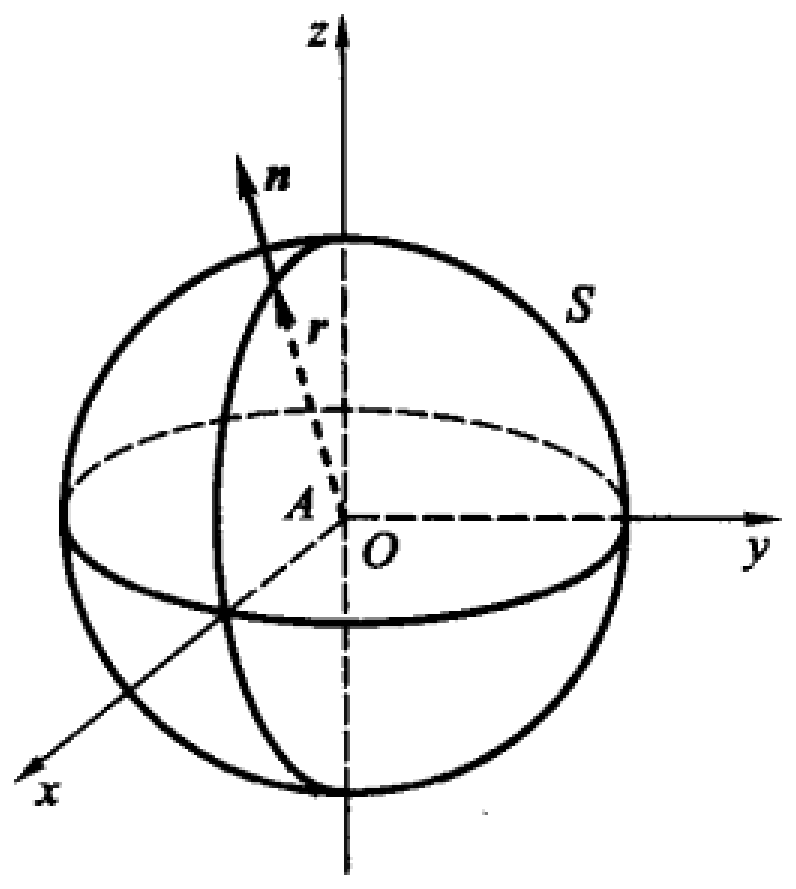
\includegraphics[width=0.28\textwidth]{work/figures/fig22-22}\caption{\relax}\label{fig:22-22}
\end{figure}

\begin{proof}[解]
\[
\frac{\partial u}{\partial x}=-\frac{m}{r^{2}}\frac{\partial r}{\partial x}=-\frac{m}{r^{2}}\frac{x}{r}.
\]
由 $x$，$y$，$z$ 的对称性得
\[
\mathrm{grad}\,u=-\frac{m}{r^{2}}\left(\frac{x}{r},\frac{y}{r},\frac{z}{r}\right)=-\frac{m}{r^{2}}\bm{r}_{0}.
\]
这里 $\bm{r}_{0}$ 是 $\bm{r}$ 方向的单位向量．上式的右端在数量上的大小恰好是两质点间的引力，方向指向原点．它表明引力场是数量场 $\dfrac{m}{r}$ 的梯度场．因此 $\dfrac{m}{r}$ 常被称为引力势．
\end{proof}

\subsection{散度场}

设 $\bm{F}(x,y,z)=\left(P(x,y,z),Q(x,y,z),R(x,y,z)\right)$ 是展布在空间某区域 $V$ 上的向量场，函数 $P$，$Q$，$R$ 在 $V$ 上存在对各变元的连续偏导数，则在 $V$ 上每一点 $(x,y,z)$，数量函数
\[
\frac{\partial P}{\partial x}+\frac{\partial Q}{\partial y}+\frac{\partial R}{\partial z}
\]
称为向量场 $\bm{F}(x,y,z)$ 在 $(x,y,z)$ 处的\emph{散度}，记作
\[
\mathrm{div}\,\bm{F}(x,y,z)=\frac{\partial P}{\partial x}+\frac{\partial Q}{\partial y}+\frac{\partial R}{\partial z}
\]
（$\mathrm{div}$ 是 divergence 的缩写），当 $(x,y,z)$ 取遍 $V$ 的点时，散度也就构成了 $V$ 的一个数量场——散度场 $\mathrm{div}\,\bm{F}(x,y,z)$．

散度场 $\mathrm{div}\,\bm{F}(x,y,z)$ 是由向量场 $\bm{F}(x,y,z)$ 产生的数量场，沿用前面提到的哈密顿算子，则散度又可表为向量 $\nabla$ 与向量 $\bm{F}$ 的内积，即
\[
\mathrm{div}\,\bm{F}(x,y,z)=\nabla\cdot\bm{F}.
\]
利用散度，高斯公式
\[
\begin{aligned}
&\iiint_{V}\left(\frac{\partial P}{\partial x}+\frac{\partial Q}{\partial y}+\frac{\partial R}{\partial z}\right)\mathrm{d}x\mathrm{d}y\mathrm{d}z\\
=&\oiint_{S}\left(P\mathrm{d}y\mathrm{d}z+Q\mathrm{d}z\mathrm{d}x+R\mathrm{d}x\mathrm{d}y\right)
\end{aligned}
\]
可以表示为向量形式：
\[
\iiint_{V}\mathrm{div}\,\bm{F}(x,y,z)\mathrm{d}x\mathrm{d}y\mathrm{d}z=\oiint_{S}\bm{F}\cdot\mathrm{d}\bm{S}.
\]
下面我们根据高斯公式，给出散度的另一种解释．对 $V$ 中任意点 $M_{0}(x_{0},y_{0},z_{0})$，取 $V_{1}$ 为包含 $M_{0}$ 的小区域，$S$ 是其边界曲面（取外侧），则上式仍成立．对上式左端的三重积分用中值定理，知存在 $M^{*}\in V_{1}$，使得
\[
\mathrm{div}\,\bm{F}(M^{*})\left|V_{1}\right|=\oiint_{S}\bm{F}\cdot\mathrm{d}\bm{S}.
\]
令 $V_{1}$ 收缩到 $M_{0}$，即对 $M_{0}\in V_{1}$，令 $d(V_{1})\to 0$，此时 $M^{*}\to M_{0}$，因此
\[
\mathrm{div}\,\bm{F}(M_{0})=\lim_{\substack{d(V_{1})\to 0\\ M_{0}\in V_{1}}}\mathrm{div}\,\bm{F}(M^{*})=\lim_{\substack{d(V_{1})\to 0\\ M_{0}\in V_{1}}}\frac{\displaystyle\oiint_{S}\bm{F}\cdot\mathrm{d}\bm{S}}{\left|V_{1}\right|}.
\]
上式有一种力学的解释．如果 $\bm{F}$ 是流体的流速场，则第二十一章 §2 的讨论告诉我们，$\displaystyle\oiint_{S}\bm{F}\cdot\mathrm{d}\bm{S}$ 是流速为 $\bm{F}$ 的流体在单位时间内流过曲面 $S$ 的流量，而 $\dfrac{1}{\left|V_{1}\right|}\displaystyle\oiint_{S}\bm{F}\cdot\mathrm{d}\bm{S}$ 便是 $V_{1}$ 内的平均流量，即在平均的意义下，单位体积流出的流量．因此其极限 $\mathrm{div}\,\bm{F}(M_{0})$ 就是流体在 $M_{0}$ 点的单位体积的流量，也就是流体速度场 $\bm{F}$ 在 $M_{0}$ 点的流量密度．显然，这个物理量是不依赖于坐标系的，这就说明了散度与坐标系的选取无关．

注意到高斯公式中表示流量的曲面积分是取外侧的，故若 $\mathrm{div}\,\bm{F}(M_{0})>0$，它表示在单位时间内有流体流出这一点，这时称 $M_{0}$ 点为\emph{源}（源泉）；若 $\mathrm{div}\,\bm{F}(M_{0})<0$，它表示在单位时间内有流体流入这一点，这时称 $M_{0}$ 点为\emph{汇}（渗入点、吸收点）．

有了散度的概念后，又可以反过来，给出高斯公式
\[
\iiint_{V}(\mathrm{div}\,\bm{F})\mathrm{d}V=\oiint_{S}\bm{F}\cdot\mathrm{d}\bm{S}
\]
的力学解释．这就是单位时间流出闭曲面 $S$ 的流量，等于区域内每一点渗出率（流量密度 $\mathrm{div}\,\bm{F}$ 乘体积元 $\mathrm{d}V$）的总和．这和我们的常识是吻合的．当向量场 $\bm{F}$ 在 $V$ 中每一点的散度皆为零时，即
\[
\mathrm{div}\,\bm{F}(M)\equiv 0,
\]
则 $V$ 内每一点既不是源也不是汇，这时称 $\bm{F}$ 为\emph{无源场}．

对无源场，有
\[
\oiint_{S}\bm{F}\cdot\mathrm{d}\bm{S}=0.
\]
它说明，流过 $V$ 的流量的代数和为 $0$，即流入 $V$ 的流量与流出 $V$ 的流量相互抵消，这与``无源''的直观是完全符合的．

\begin{example}\label{ex:22-3-3}
例~\ref{ex:22-3-2} 中由函数 $\dfrac{m}{r}$ 产生的梯度场为
\[
\mathrm{grad}\,u=-\frac{m}{r^{2}}\left(\frac{x}{r},\frac{y}{r},\frac{z}{r}\right),
\]
求 $\mathrm{grad}\,u$ 产生的散度场．
\end{example}

\begin{proof}[解]
记 $P(x,y,z)=-\dfrac{m}{r^{3}}x$，则
\[
\frac{\partial P}{\partial x}=-\frac{m}{r^{3}}+\frac{3mx}{r^{4}}\frac{\partial r}{\partial x}=-\frac{m}{r^{3}}+\frac{3mx}{r^{4}}\frac{x}{r}.
\]
由 $x$，$y$，$z$ 的对称性即知
\[
\mathrm{div}\,\mathrm{grad}\,u=-\frac{3m}{r^{3}}+\frac{3mx^{2}}{r^{5}}+\frac{3my^{2}}{r^{5}}+\frac{3mz^{2}}{r^{5}}=0.
\]
此例表明引力场的散度场是无源场．
\end{proof}

\subsection{旋度场}

设 $\bm{F}(x,y,z)=\left(P(x,y,z),Q(x,y,z),R(x,y,z)\right)$ 是展布在空间某区域 $V$ 上的向量场，函数 $P$，$Q$，$R$ 在 $V$ 上存在对各变元的连续偏导数，则在 $V$ 上每一点 $(x,y,z)$，向量函数
\[
\left(\frac{\partial R}{\partial y}-\frac{\partial Q}{\partial z},\ \frac{\partial P}{\partial z}-\frac{\partial R}{\partial x},\ \frac{\partial Q}{\partial x}-\frac{\partial P}{\partial y}\right)
\]
称为向量场 $\bm{F}(x,y,z)$ 在 $(x,y,z)$ 处的\emph{旋度}，记作 $\mathrm{rot}\,\bm{F}(x,y,z)$（$\mathrm{rot}$ 是 rotation 的缩写）．当 $(x,y,z)$ 取遍区域 $V$ 的点时，$\mathrm{rot}\,\bm{F}(x,y,z)$ 便定义了 $V$ 的一个向量场，称为 $\bm{F}$ 的\emph{旋度场}．旋度场 $\mathrm{rot}\,\bm{F}(x,y,z)$ 是由向量场 $\bm{F}(x,y,z)$ 产生的向量场．

为便于记忆，常把旋度表为
\[
\mathrm{rot}\,\bm{F}(x,y,z)=\begin{vmatrix}\bm{i}&\bm{j}&\bm{k}\\[3pt]\dfrac{\partial}{\partial x}&\dfrac{\partial}{\partial y}&\dfrac{\partial}{\partial z}\\[3pt] P&Q&R\end{vmatrix}=\nabla\times\bm{F},
\]
即旋度是向量 $\nabla$ 与向量 $\bm{F}$ 的外积．

利用旋度，斯托克斯公式可以表示为向量形式：
\[
\iint_{S}\mathrm{rot}\,\bm{F}\cdot\mathrm{d}\bm{S}=\oint_{L}\bm{F}\cdot\mathrm{d}\bm{s}
\]
或
\[
\iint_{S}\mathrm{rot}\,\bm{F}\cdot\bm{n}\,\mathrm{d}S=\oint_{L}\bm{F}\cdot\mathrm{d}\bm{s},
\]
其中 $\bm{n}$ 为曲面 $S$ 在规定侧的单位法向量．上式中，右边的积分
\[
\oint_{L}\bm{F}\cdot\mathrm{d}\bm{s}=\oint_{L}P\mathrm{d}x+Q\mathrm{d}y+R\mathrm{d}z
\]
称为向量场 $\bm{F}$ 沿闭曲线 $L$ 的\emph{环流量}，它反映了向量场 $\bm{F}$ 沿 $L$ 的旋转强弱程度．

与散度一样，旋度是与坐标的选取无关的．事实上，在 $M_{0}$ 点选定一个单位方向 $\bm{n}$，过 $M_{0}$ 点作平面 $\pi$ 垂直于 $\bm{n}$，在 $\pi$ 上围绕 $M_{0}$ 点作一简单封闭曲线 $L$，其方向和 $\bm{n}$ 的方向构成右手法则，$L$ 所围平面区域为 $D$，则由斯托克斯公式，有
\[
\iint_{D}\mathrm{rot}\,\bm{F}\cdot\bm{n}\,\mathrm{d}S=\oint_{L}\bm{F}\cdot\mathrm{d}\bm{s}.
\]
由二重积分中值定理，存在 $M^{*}\in D$，使得
\[
\mathrm{rot}\,\bm{F}(M^{*})\cdot\bm{n}\,|D|=\oint_{L}\bm{F}\cdot\mathrm{d}\bm{s}.
\]
令 $D$ 收缩到点 $M_{0}$，记为 $D\to M_{0}$，此时有 $M^{*}\to M_{0}$，故
\[
\mathrm{rot}\,\bm{F}(M_{0})\cdot\bm{n}=\lim_{D\to M_{0}}\frac{\displaystyle\oint_{L}\bm{F}\cdot\mathrm{d}\bm{s}}{|D|}.
\]
这公式说明，$\bm{F}$ 在 $M_{0}$ 的旋度在 $\bm{n}$ 方向的投影 $\mathrm{rot}\,\bm{F}(M_{0})\cdot\bm{n}$ 等于在 $M_{0}$ 的单位面积的环流量，显然这个物理量是不依赖于坐标系的．只要知道向量 $\mathrm{rot}\,\bm{F}(M_{0})$ 在任意方向 $\bm{n}$ 上的投影，便完全确定了向量 $\mathrm{rot}\,\bm{F}(M_{0})$ 的本身．因此旋度与坐标系的选取无关．

如果在 $V$ 中每一点 $M$，有 $\mathrm{rot}\,\bm{F}(M)\equiv 0$，则称 $\bm{F}$ 为\emph{无旋场}．

为了进一步说明旋度的物理意义，我们来看刚体以固定的角速度 $\bm{\omega}$ 绕某过原点的轴旋转．这时角速度 $\bm{\omega}$ 的方向平行于旋转轴，线速度 $\bm{v}$ 与 $\bm{\omega}$ 构成右手法则，且
\[
\begin{aligned}
\bm{v}=\bm{\omega}\times\bm{r}&=\begin{vmatrix}\bm{i}&\bm{j}&\bm{k}\\ \omega_{x}&\omega_{y}&\omega_{z}\\ x&y&z\end{vmatrix}\\
&=\left(z\omega_{y}-y\omega_{z}\right)\bm{i}+\left(x\omega_{z}-z\omega_{x}\right)\bm{j}+\left(y\omega_{x}-x\omega_{y}\right)\bm{k}.
\end{aligned}
\]
\begin{figure}[htbp]
\centering
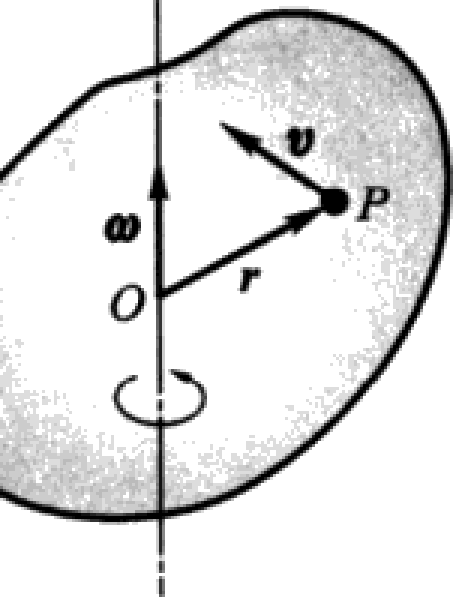
\includegraphics[width=0.22\textwidth]{work/figures/fig22-23}\caption{\relax}\label{fig:22-23}
\end{figure}
我们来计算速度场 $\bm{v}$ 的旋度，得
\[
\mathrm{rot}\,\bm{v}=\begin{vmatrix}\bm{i}&\bm{j}&\bm{k}\\[3pt]\dfrac{\partial}{\partial x}&\dfrac{\partial}{\partial y}&\dfrac{\partial}{\partial z}\\[3pt] z\omega_{y}-y\omega_{z}&x\omega_{z}-z\omega_{x}&y\omega_{x}-x\omega_{y}\end{vmatrix}=2\bm{\omega}.
\]
上式表明线速度 $\bm{v}$ 的旋度 $\mathrm{rot}\,\bm{v}$ 等于角速度 $\bm{\omega}$ 的二倍．当角速度 $\bm{\omega}\equiv 0$ 时，刚体无旋转，$\mathrm{rot}\,\bm{v}\equiv 0$．这说明向量场 $\bm{F}$ 的旋度 $\mathrm{rot}\,\bm{F}$ 反映了 $\bm{F}$ 在一点附近的旋转强弱的程度与方向．

\subsection{\texorpdfstring{梯度、散度、旋度等于零的充要条件}{梯度、散度、旋度等于零的充要条件}}

\begin{theorem}\label{thm:22-6}
设 $V$ 是空间某单连通区域，$u(x,y,z)$ 在 $V$ 内有连续偏导数，则在 $V$ 内，$\mathrm{grad}\,u\equiv 0$ 的充要条件是数量场 $u(x,y,z)$ 是常量场．
\end{theorem}

\begin{proof}
充分性显然成立，下证必要性．由 $\mathrm{grad}\,u=\bm{0}$，即
\[
\frac{\partial u}{\partial x}=\frac{\partial u}{\partial y}=\frac{\partial u}{\partial z}\equiv 0.
\]
设 $M_{1}$ 和 $M_{2}$ 是 $V$ 内任意两点，则在 $V$ 内任一从 $M_{1}$ 到 $M_{2}$ 的逐段光滑曲线 $L$，曲线积分
\[
\int_{L}\frac{\partial u}{\partial x}\mathrm{d}x+\frac{\partial u}{\partial y}\mathrm{d}y+\frac{\partial u}{\partial z}\mathrm{d}z=\int_{L}\mathrm{d}u\equiv 0.
\]
而
\[
\int_{L}\mathrm{d}u=\int_{M_{1}}^{M_{2}}\mathrm{d}u=u(M_{2})-u(M_{1}),
\]
因此
\[
u(M_{1})\equiv u(M_{2}).
\]
由 $M_{1}$ 和 $M_{2}$ 的任意性即知 $u$ 是常量场．定理~\ref{thm:22-6} 证完．
\end{proof}

\begin{theorem}\label{thm:22-7}
设 $\Omega$ 是空间单连通区域，$\bm{F}=(P,Q,R)$ 是展布在 $\Omega$ 上的向量场，$P$，$Q$，$R$ 在 $\Omega$ 内有连续的偏导数，则在 $\Omega$ 内 $\mathrm{div}\,\bm{F}(x,y,z)\equiv 0$ 的充要条件是对 $\Omega$ 内任一分片光滑的封闭曲面 $S$，有 $\displaystyle\oiint\bm{F}\cdot\mathrm{d}\bm{S}=0$．
\end{theorem}

\begin{proof}
必要性．对 $\Omega$ 内任一分片光滑封闭曲面 $S$，由高斯公式立得
\[
\oiint_{S}\bm{F}\cdot\mathrm{d}\bm{S}=\iiint_{V}\mathrm{div}\,\bm{F}(M)\mathrm{d}V=0.
\]
充分性，对任意 $M_{0}\in\Omega$，取 $V$ 为以 $M_{0}$ 为中心半径为 $r$ 的球体，$S$ 是它的边界球面，则由散度的公式知
\[
\mathrm{div}\,\bm{F}(M_{0})=\lim_{V\to M_{0}}\frac{\displaystyle\oiint_{S}\bm{F}\cdot\mathrm{d}\bm{S}}{|V|}=0.
\]
定理~\ref{thm:22-7} 证完．
\end{proof}

满足定理~\ref{thm:22-7} 中必要条件的场 $\bm{F}$ 称为\emph{管量场}，因此定理~\ref{thm:22-7} 又可叙述为 $\bm{F}$ 是无源场的充要条件为 $\bm{F}$ 是管量场．

在向量场 $\bm{F}=(P,Q,R)$ 中，如果曲线上每一点的切线平行于该点的场向量 $\bm{F}$，即
\[
\frac{\mathrm{d}x}{P}=\frac{\mathrm{d}y}{Q}=\frac{\mathrm{d}z}{R},
\]
则称曲线 $L$ 为向量场的\emph{向量线}．由向量线围成的管状曲面称为\emph{向量管}．在向量管上任取两断面 $S_{1}$，$S_{2}$，以 $S_{3}$ 表示截出的管的侧表面，则 $S=S_{1}\cup S_{2}\cup S_{3}$ 是一封闭曲面，因为曲面 $S_{3}$ 的法向量垂直于 $\bm{F}$，因此
\[
\iint_{S_{3}}\bm{F}\cdot\mathrm{d}\bm{S}=\iint_{S_{3}}\bm{F}\cdot\bm{n}\,\mathrm{d}S=0,
\]
\begin{figure}[htbp]
\centering
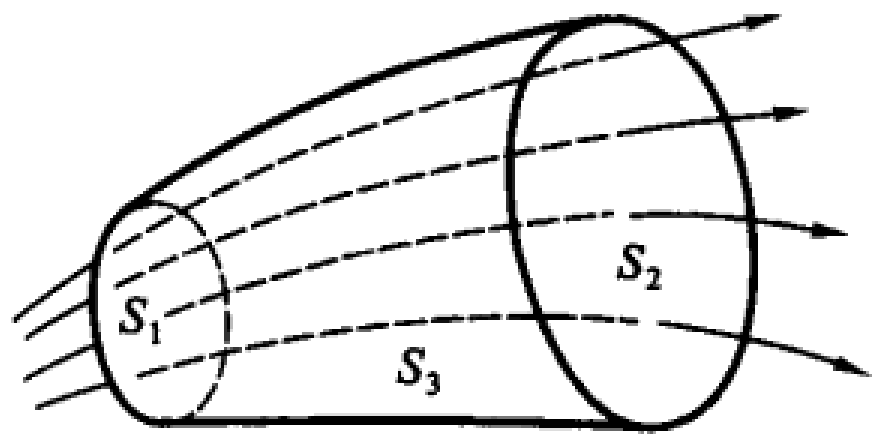
\includegraphics[width=0.32\textwidth]{work/figures/fig22-24}\caption{\relax}\label{fig:22-24}
\end{figure}
从而对 $S$ 的外侧，
\[
\oiint_{S}\bm{F}\cdot\mathrm{d}\bm{S}=0
\]
当且仅当
\[
\left(\iint_{S_{1}}+\iint_{S_{2}}\right)\bm{F}\cdot\mathrm{d}\bm{S}=0.
\]
即
\[
\iint_{S_{2}}\bm{F}\cdot\mathrm{d}\bm{S}=-\iint_{S_{1}}\bm{F}\cdot\mathrm{d}\bm{S}.
\]
可见管量场的物理意义是流体通过向量管的任意断面的流量相等．这也是管量场名称的由来．

最后我们讨论旋度等于零的充要条件．其实，它就是定理~\ref{thm:22-5} 中积分与路径无关的四个等价条件．

设 $V$ 是空间的单连通区域，$\bm{F}=(P,Q,R)$ 是展布在 $V$ 上的向量场，$P$，$Q$，$R$ 在 $V$ 内有连续偏导数，若对 $V$ 内任一逐段光滑封闭曲线 $L$，有
\[
\oint_{L}\bm{F}\cdot\mathrm{d}\bm{s}=0,
\]
则称 $\bm{F}$ 是\emph{有势场}．若对 $V$ 内任一逐段光滑曲线 $L$，有 $\displaystyle\int_{L}\bm{F}\cdot\mathrm{d}\bm{s}$ 与路径无关，则称 $\bm{F}$ 是\emph{保守场}．这样定理~\ref{thm:22-5} 又可叙述为：

\begin{theorem}\label{thm:22-8}
设 $V$ 是空间的单连通区域，$\bm{F}=(P,Q,R)$ 在 $V$ 内有连续偏导数，则下列四条件等价：
\begin{enumerate}[label=（\arabic*）]
\item $\bm{F}$ 是有势场；
\item $\bm{F}$ 是保守场；
\item $\bm{F}$ 是梯度场；
\item $\bm{F}$ 是无旋场．
\end{enumerate}
\end{theorem}

例~\ref{ex:22-3-3} 中已证
\[
\mathrm{div}\,\mathrm{grad}\left(\frac{m}{r}\right)=0.
\]
即 $\bm{F}=\mathrm{grad}\left(\dfrac{m}{r}\right)$ 是无源场，从而是管量场．又由 $\bm{F}$ 的定义知 $\bm{F}$ 是梯度场，这又等价于 $\bm{F}$ 是有势场、保守场和无旋场．

一个向量场 $\bm{F}$ 若同时是管量场和有势场，则称这个向量场为\emph{调和场}．这时存在势函数 $u$，满足
\[
\bm{F}=\mathrm{grad}\,u,\qquad\mathrm{div}\,\mathrm{grad}\,u=0.
\]
它等价于
\[
\frac{\partial^{2}u}{\partial x^{2}}+\frac{\partial^{2}u}{\partial y^{2}}+\frac{\partial^{2}u}{\partial z^{2}}=0.
\]
这时函数 $u$ 称为\emph{调和函数}．

例~\ref{ex:22-3-3} 表明 $\dfrac{m}{r}$ 是调和函数．

根据上面的讨论易知，对任意向量场 $\bm{A}$，有

（1）$\mathrm{div}\,\mathrm{rot}\,\bm{A}=\bm{0}$；

（2）$\mathrm{rot}\,\mathrm{grad}\,u=\bm{0}$．

我们把证明留给读者．

\begin{xiti}
\item 求 $u=x^{2}+2y^{2}+3z^{2}+2xy-4x+2y-4z$ 在点 $O(0,0,0)$，$A(1,1,1)$，$B(-1,-1,-1)$ 的梯度，并求梯度为零的点．
\item 计算下列向量场 $\bm{F}$ 的散度和旋度：
\begin{ziti}
\item $\bm{F}=(y^{2}+z^{2},\,z^{2}+x^{2},\,x^{2}+y^{2})$；
\item $\bm{F}=(x^{2}yz,\,xy^{2}z,\,xyz^{2})$；
\item $\bm{F}=\left(\dfrac{x}{yz},\,\dfrac{y}{zx},\,\dfrac{z}{xy}\right)$．
\end{ziti}
\item 证明 $\bm{F}=(yz(2x+y+z),\,xz(x+2y+z),\,xy(x+y+2z))$ 是有势场并求势函数．
\item 设 $P=x^{2}+5\lambda y+3yz$，$Q=5x+3\lambda xz-2$，$R=(\lambda+2)xy-4z$．
\begin{ziti}
\item 计算 $\displaystyle\int_{L}P\mathrm{d}x+Q\mathrm{d}y+R\mathrm{d}z$，其中 $L$ 是螺旋线 $x=a\cos t$，$y=a\sin t$，$z=ct$（$0\leqslant t\leqslant 2\pi$）；
\item 设 $\bm{F}=(P,Q,R)$，求 $\mathrm{rot}\,\bm{F}$；
\item 在什么条件下 $\bm{F}$ 为有势场，并求势函数．
\end{ziti}
\item 设 $\varphi$ 为可微函数，$\bm{r}=(x,y,z)$，$r=|\bm{r}|$，求 $\mathrm{grad}\,\varphi(r)$，$\mathrm{div}\,(\varphi(r)\bm{r})$，$\mathrm{rot}\,(\varphi(r)\bm{r})$．
\item 求向量场 $\bm{F}=(-y,x,z)$ 沿曲线 $L$ 的环流量：
\begin{ziti}
\item $L$ 为 $Oxy$ 平面上的圆周 $x^{2}+y^{2}=1$，$z=0$，逆时针方向；
\item $L$ 为 $Oxy$ 平面上的圆周 $(x-2)^{2}+y^{2}=R^{2}$，$z=0$，逆时针方向；
\item $L$ 为 $Oxy$ 平面上任一逐段光滑简单闭曲线，它围成的平面区域 $D$ 的面积为 $S$．证明 $\bm{F}$ 沿 $L$ 的环流量为 $2S$；
\item 设有一平面 $\pi$：$ax+by+cz=d$（$c\neq 0$），取 $\pi$ 为上侧，$\pi$ 上有一逐段光滑简单闭曲线 $L$，其方向关于 $\pi$ 为正向．$L$ 围成的平面区域的面积为 $S$，问 $\bm{F}$ 沿 $L$ 的环流量是什么？
\end{ziti}
\item 求向量场 $\bm{F}=\mathrm{grad}\left(\arctan\dfrac{y}{x}\right)$ 沿曲线 $L$ 的环流量：（1）$L$ 不环绕 $z$ 轴；（2）$L$ 环绕 $z$ 轴一圈；（3）$L$ 环绕 $z$ 轴 $n$ 圈．
\item 设向量场 $\bm{F}=(P,Q,R)$ 在除原点 $(0,0,0)$ 外有连续的偏导数，在球面 $x^{2}+y^{2}+z^{2}=t^{2}$ 上 $\bm{F}$ 的长度保持一固定值，$\bm{F}$ 的方向与矢径 $\bm{r}=(x,y,z)$ 相同，而且 $\bm{F}$ 的散度恒为零，证明此向量场为 $\bm{F}=\dfrac{k}{r^{3}}\bm{r}$（$k$ 是常数）．
\item 设有一数量场 $u(x,y,z)$，除 $(0,0,0)$ 点外有连续偏导数，其等值面是以原点为中心的球面．又数量场的梯度场的散度为零，证明此数量场与 $\dfrac{c_{1}}{r}$（$r=\sqrt{x^{2}+y^{2}+z^{2}}$）仅差一个常数，其中 $c_{1}$ 为某固定常数．
\item 设 $G$ 是空间开区域，$u(x,y,z)$ 在 $G$ 上有二阶连续偏导数．证明 $u(x,y,z)$ 在 $G$ 内调和的充要条件是对 $G$ 内任一简单分片光滑曲面 $S$，都有
\[
\iint_{S}\frac{\partial u}{\partial n}\mathrm{d}S=0.
\]
\end{xiti}


\end{document}
